\documentclass[10pt,onecolumn,letterpaper]{article}
\usepackage[textwidth=7.16in,textheight=9.45in,columnsep=0.17in,top=0.65in]{geometry}
\usepackage{mathptmx}
\usepackage{titlesec}
\titleformat{\section}{\centering\scshape\normalsize}{\Roman{section}.}{0.5em}{}
\titleformat{\subsection}{\itshape\normalsize}{\Alph{subsection}.}{0.5em}{}
\titlespacing*{\section}{0pt}{1.2ex}{0.6ex}
\titlespacing*{\subsection}{0pt}{1ex}{0.4ex}
\usepackage[font=footnotesize,labelfont=sc]{caption}
\setlength{\parskip}{0pt}
\newcommand{\IEEEPARstart}[2]{#1#2}
\newcommand{\IEEEmembership}[1]{}
\newenvironment{IEEEkeywords}{\par\footnotesize\textbf{\textit{Index Terms}---}}{\par}
\newenvironment{IEEEproof}[1][Proof]{\par\textit{#1:}}{\par}
\newenvironment{IEEEbiographynophoto}[1]{\par\textbf{#1}}{\par}
\newcommand{\appendices}{\appendix}
\let\oldabstract\abstract
\renewenvironment{abstract}{\par\footnotesize\textbf{\textit{Abstract}---}}{\par}

\usepackage{longtable}
\extrafloats{300}
\usepackage{amsmath,amsfonts,amssymb}
\usepackage{algorithmic}
\usepackage{algorithm}
\usepackage{array}
\usepackage[caption=false]{subfig}
\usepackage{textcomp}
\usepackage{stfloats}
\usepackage{url}
\usepackage{verbatim}
\usepackage{graphicx}
\usepackage{cite}
\usepackage{booktabs}
\usepackage{multirow}
\usepackage{xcolor}
\usepackage{tikz}
\usetikzlibrary{positioning,arrows.meta,fit,backgrounds,calc}
\hyphenation{op-tical net-works semi-conduc-tor IEEE-Xplore}

\newcommand{\placeholderfig}[2]{%
  \framebox{\parbox[c][#2][c]{#1}{\centering\small\textit{Figure placeholder}}}}
\newcommand{\resultfig}[3]{%
  \begin{figure}[!t]\centering
  \IfFileExists{figures/#1.pdf}{\includegraphics[width=0.95\columnwidth]{figures/#1.pdf}}%
    {\placeholderfig{0.9\columnwidth}{1.6in}}
  \caption{#2}\label{#3}\end{figure}}

\newtheorem{definition}{Definition}
\newtheorem{lemma}{Lemma}
\newtheorem{proposition}{Proposition}
\newtheorem{corollary}{Corollary}
\newtheorem{remark}{Remark}

\newcommand{\U}{\mathcal{U}}
\newcommand{\G}{\mathcal{G}}
\newcommand{\AR}{\mathrm{AR}}
\newcommand{\FAR}{\mathrm{FAR}}
\newcommand{\TPR}{\mathrm{TPR}}
\newcommand{\Lap}{\mathrm{Lap}}
\newcommand{\Prob}{\Pr}
\newcommand{\ind}{\mathbb{1}}

\begin{document}

\title{Extended Results for ``Who Gets Suspected, and Who Gets Away? Burden and Evasion in History-Dependent Insider-Risk Alerting''}

\author{Rim~Ben~Salem}

\markboth{IEEE Transactions on Dependable and Secure Computing}%
{Ben Salem: Extended Results}

\maketitle

\renewcommand{\thesection}{E-\Roman{section}}
\renewcommand{\thetable}{E\arabic{table}}
\renewcommand{\thefigure}{E\arabic{figure}}
\renewcommand{\thealgorithm}{E\arabic{algorithm}}
\renewcommand{\theproposition}{E\arabic{proposition}}
\renewcommand{\thelemma}{S\arabic{lemma}}
\renewcommand{\theequation}{E\arabic{equation}}

This document archives the extended results of the paper, with every table produced by the notebooks of the archive. Equations, propositions and sections without the prefix E refer to the main paper, and those with the prefix S to its supplementary material. Sections E-I to E-VI report the full experiments in which a timing attack moves the insider's scores without recomputing them and farming uses the insider's mean profile without a cap; the main paper's attack results use behavioral relocation and rescoring, whose full results are in Section~\ref{sec:e-rev8}. Both constructions give excess losses of similar size.

\section{Formal Results Not in the Main Paper}
\label{sec:s-proof}

\subsection{The Exact Parity Rule}
With the notation of Section~V-B of the main paper, the exact rule solves
\begin{align}
\max_{\{k_g\}}\;& \sum_{g\in\G} S_g(k_g),\quad S_g(k_g)=\sum_{j=1}^{k_g}s_{(j),g} \label{eq:s-obj}\\
\text{s.t.}\;& \sum_{g}k_g=k,\quad 0\le k_g\le n_g, \label{eq:s-budget}\\
& \left|\frac{A_g+k_g}{D_g}-\frac{A_h+k_h}{D_h}\right|\le\delta\quad\forall g,h\in\G. \label{eq:s-parity}
\end{align}
Constraint \eqref{eq:s-parity} holds if and only if there exists $r\in[0,1]$ such that $(A_g+k_g)/D_g\in[r,r+\delta]$ for all $g$. For fixed $r$, the problem becomes
\begin{equation}
\max\sum_g S_g(k_g)\;\;\text{s.t.}\;\sum_g k_g=k,\;\; L_g(r)\le k_g\le U_g(r),
\label{eq:s-fixedr}
\end{equation}
with $L_g(r)=\max\{0,\lceil rD_g-A_g\rceil\}$ and $U_g(r)=\min\{n_g,\lfloor (r+\delta)D_g-A_g\rfloor\}$.

\begin{proposition}[Exact allocation]
\label{prop:s-greedy}
(i) For fixed $r$, problem \eqref{eq:s-fixedr} is solved exactly by setting $k_g=L_g(r)$ and then alerting the $k-\sum_gL_g(r)$ highest scores among the candidates $\{s_{(j),g}: L_g(r)<j\le U_g(r)\}$; $r$ is infeasible if $\sum_g L_g(r)>k$ or $\sum_g U_g(r)<k$. (ii) Let $\mathcal{R}$ be the set of points $(A_g+j)/D_g$, $g\in\G$, $j=0,\dots,n_g$, that lie in $[0,\bar r]$, with $\bar r=(k+\sum_gA_g)/\sum_gD_g$. Evaluating (i) for every $r\in\mathcal{R}$ and keeping the best feasible solution solves \eqref{eq:s-obj}--\eqref{eq:s-parity} exactly. This holds for real-valued $A_g$ and $D_g$, and hence for the discounted history.
\end{proposition}

The objective is a standard separable concave resource-allocation problem \cite{ibaraki1988resource}; the implementation matched exhaustive search on $1{,}500$ random instances and takes a few milliseconds per day. If $\{K_g\}$ satisfies \eqref{eq:s-parity}, the global top-$k$ set is the unique optimum, which gives the last statement of Proposition~2 of the main paper.

\begin{IEEEproof}
Throughout, $s_{(1),g}\ge\dots\ge s_{(n_g),g}$ and $S_g(k)=\sum_{j\le k}s_{(j),g}$, so that the marginal gain of the $j$-th alert in group $g$ is $\Delta_g(j)=S_g(j)-S_g(j-1)=s_{(j),g}$, which is non-increasing in $j$.

\emph{Part (i).} Fix $r$ and the boxes $L_g\le k_g\le U_g$, and assume $\sum_gL_g\le k\le\sum_gU_g$. Let $m=k-\sum_gL_g$ and let $\mathcal{P}=\{(g,j):L_g<j\le U_g\}$ be the candidate pool, with value $s_{(j),g}$ for $(g,j)$. Any feasible $\{k_g\}$ corresponds to the subset $\mathcal{Q}(k)=\{(g,j):L_g<j\le k_g\}\subseteq\mathcal{P}$ of size $m$, and its objective is $\sum_gS_g(L_g)+\sum_{(g,j)\in\mathcal{Q}(k)}s_{(j),g}$. The first term does not depend on $k$. Hence the problem is to choose $m$ elements of $\mathcal{P}$ that form a prefix within each group and have maximum total value.

Let $\mathcal{T}$ be a set of $m$ elements of $\mathcal{P}$ with the largest values, ties broken by smaller $j$ within a group. We first show that $\mathcal{T}$ is a prefix within each group. Suppose $(g,j)\in\mathcal{T}$ and $(g,j')\notin\mathcal{T}$ with $L_g<j'<j$. Then $s_{(j'),g}\ge s_{(j),g}$; if the inequality is strict, $\mathcal{T}$ does not contain the $m$ largest values, and if it is an equality, the tie-breaking rule is violated. Both are contradictions, so $\mathcal{T}=\mathcal{Q}(k^\star)$ for some feasible $k^\star$.

We now show that $k^\star$ is optimal. Let $k$ be any feasible allocation with $k\ne k^\star$. Since $\sum_gk_g=\sum_gk^\star_g$, there exist groups $g,h$ with $k_g<k^\star_g$ and $k_h>k^\star_h$. Consider $k'$ obtained from $k$ by adding one alert to $g$ and removing one from $h$; it is feasible because $L_g\le k_g<k^\star_g\le U_g$ and $U_h\ge k_h>k^\star_h\ge L_h$. Its objective changes by $s_{(k_g+1),g}-s_{(k_h),h}$. Now $(g,k_g+1)\in\mathcal{T}$ because $k_g+1\le k^\star_g$, and $(h,k_h)\notin\mathcal{T}$ because $k_h>k^\star_h$. Since $\mathcal{T}$ contains the $m$ largest values of $\mathcal{P}$, $s_{(k_g+1),g}\ge s_{(k_h),h}$, so the objective does not decrease. Each such exchange reduces $\sum_g|k_g-k^\star_g|$ by $2$, so after finitely many exchanges we reach $k^\star$ without ever decreasing the objective. Hence $\sum_gS_g(k^\star_g)\ge\sum_gS_g(k_g)$ for every feasible $k$, which proves (i). If $\sum_gL_g>k$ or $\sum_gU_g<k$, no allocation satisfies the boxes and the budget simultaneously, so $r$ is infeasible.

\emph{Part (ii).} An allocation $\{k_g\}$ satisfies \eqref{eq:s-parity} if and only if $\max_g R_g-\min_g R_g\le\delta$, where $R_g=(A_g+k_g)/D_g$, i.e., if and only if there exists $r$ with $R_g\in[r,r+\delta]$ for all $g$ (take $r=\min_gR_g$). For a given $r$, $R_g\in[r,r+\delta]$ is equivalent to $\lceil rD_g-A_g\rceil\le k_g\le\lfloor(r+\delta)D_g-A_g\rfloor$, which, combined with $0\le k_g\le n_g$, gives the boxes $[L_g(r),U_g(r)]$ of \eqref{eq:s-fixedr}, or infeasibility if $\lceil rD_g-A_g\rceil>n_g$ or $\lfloor(r+\delta)D_g-A_g\rfloor<0$. Therefore the feasible set of \eqref{eq:s-obj}--\eqref{eq:s-parity} is the union over $r\ge0$ of the feasible sets of \eqref{eq:s-fixedr}, and its optimum is the maximum over $r$ of the optima of \eqref{eq:s-fixedr}.

It remains to show that the finite set $\mathcal{R}$ suffices. Every $r$ gives a restriction of the original problem, so the best value over $r\in\mathcal{R}$ is at most the optimum. Conversely, let $k^\star$ be an optimal allocation and $r^\star=\min_gR_g=(A_{g^\star}+k^\star_{g^\star})/D_{g^\star}$. Then $r^\star$ has the form $(A_g+j)/D_g$ with $0\le j\le n_g$, and $k^\star$ satisfies the boxes $[L_g(r^\star),U_g(r^\star)]$ and the budget, so \eqref{eq:s-fixedr} is feasible at $r^\star$, which forces $r^\star\le\bar r$ because $k\ge\sum_gL_g(r^\star)\ge r^\star\sum_gD_g-\sum_gA_g$. Hence $r^\star\in\mathcal{R}$, and by (i) the value of \eqref{eq:s-fixedr} at $r^\star$ is at least that of $k^\star$. The best value over $\mathcal{R}$ is therefore the optimum of \eqref{eq:s-obj}--\eqref{eq:s-parity}. Nothing in this argument uses integrality of $A_g$ or $D_g$. At $r=(A_g+j)/D_g$, the quantity $rD_g-A_g$ equals the integer $j$, and floating-point rounding could make $\lceil rD_g-A_g\rceil=j+1$ and wrongly exclude $r$; the implementation therefore evaluates $\lceil x-10^{-9}\rceil$ and $\lfloor x+10^{-9}\rfloor$. It also evaluates the points $(A_g+j)/D_g-\delta$ and the midpoints between consecutive points, which is redundant but harmless. \hfill$\blacksquare$

\end{IEEEproof}

\subsection{Soundness of Private Certificates}
The oversight body certifies window $w$ as $\delta_{\mathrm{rep}}$-fair if $\widetilde{\Delta}_{\AR}=\max_{g,h}|\widetilde{\AR}_g-\widetilde{\AR}_h|\le\delta_{\mathrm{rep}}$, where $\widetilde{\AR}_{g,w}=\tilde c_{g,w}/R_g$ and $\AR_g$, $\FAR_g$ and $\pi_g$ are employee-level quantities within the window.

\begin{proposition}[Soundness of private certificates]
\label{prop:s-dp}
Let $R_{\min}$ be the smallest roster. For any $\beta\in(0,1)$, with probability at least $1-\beta$ over the noise,
\begin{equation}
\Delta_{\FAR}\le\widetilde{\Delta}_{\AR}+\frac{2\ln(|\G|/\beta)}{\varepsilon\,R_{\min}}+2\pi_{\max}.
\label{eq:s-dpbound}
\end{equation}
\end{proposition}
\begin{IEEEproof}
For $Z\sim\Lap(\ell)$, $\Prob(|Z|>\ell\ln(1/\beta'))=\beta'$. Setting $\beta'=\beta/|\G|$ and applying a union bound over groups, with probability at least $1-\beta$, $|\widetilde{\AR}_g-\AR_g|\le\ln(|\G|/\beta)/(\varepsilon R_g)$ for all $g$. Hence $\Delta_{\AR}\le\widetilde{\Delta}_{\AR}+2\ln(|\G|/\beta)/(\varepsilon R_{\min})$, and Lemma~S1 of the supplementary material completes the proof.
\end{IEEEproof}

We call the middle term of \eqref{eq:s-dpbound} the \emph{certificate slack}. At our group sizes, the certificate is vacuous: with $\varepsilon=1$, $\beta=0.05$ and functional units, the slack is $2\ln(100)/34=0.27$ on r4.2 ($|\G|=5$, $R_{\min}=34$) and $2\ln(140)/6=1.65$ on r5.2 ($|\G|=7$, $R_{\min}=6$), against observed disparities below $0.06$. The proposition states what a report can certify for larger groups; it requires $R_{\min}\ge2\ln(|\G|/\beta)/(\varepsilon\,\bar\Delta)$ for a slack $\bar\Delta$, for example $R_{\min}\ge185$ for $\bar\Delta=0.05$ with five groups. With roster denominators, it depends neither on the window length nor on day-to-day activity, and shrinks only with the smallest roster and with $\varepsilon$. Frequent reports call for tighter accounting \cite{bun2016concentrated} or the tree mechanism \cite{dwork2010continual,chan2011private}.

\section{Experimental Details}
\label{sec:s-features}
This section details the experimental design summarized in Section~VI of the main paper. Table~\ref{tab:s-datasets} gives the statistics of the two CERT releases.

\begin{table}[!t]
\caption{Dataset Statistics (Active User-Days, Temporal Split)\label{tab:s-datasets}}
\centering
\resizebox{\columnwidth}{!}{%
\begin{tabular}{lccccccccc}
\toprule
Release & Users & Insiders & Test ins. & Days & User-days & $\pi$ & Roles & Func. units & Split \\
\midrule
r4.2 & 1,000 & 70 & 51 & 501 & 330,452 & 0.29\% & 42 & 7 & 2010-09-09 \\
r6.2 & 4,000 & 5 & 3 & 516 & 1,394,010 & 0.0032\% & 46 & 11 & 2010-09-17 \\
\bottomrule
\end{tabular}}
\end{table}

\subsection{Feature Definitions}
Table~\ref{tab:s-features} defines the 27 count features computed per user-day, plus the weekend indicator. After hours means before 8:00, after 18:00, or on a weekend. Keyword matches are case-insensitive substring matches on the URL. The job-search list is \textit{job, career, monster, indeed, simplyhired, hire, recruit, linkedin, resume}; the leak-site list is \textit{wikileaks, leak}; and the cloud-storage list is \textit{dropbox, drive.google, box.com, onedrive, mega., wetransfer, 4shared, mediafire}. An e-mail is external if at least one recipient (to, cc or bcc) is outside the organization's domain (\textit{dtaa.com} in CERT). In r6.2, only e-mails whose activity is \textit{Send} are counted.

\begin{table}[!t]
\caption{User-Day Features\label{tab:s-features}}
\centering
\footnotesize
\begin{tabular}{@{}llp{4.6cm}@{}}
\toprule
Source & Feature & Definition \\
\midrule
logon  & \texttt{logon\_n}   & number of logons \\
       & \texttt{logoff\_n}  & number of logoffs \\
       & \texttt{logon\_ah}  & logons after hours \\
       & \texttt{pc\_n}      & distinct PCs used \\
device & \texttt{dev\_n}     & removable-device connections \\
       & \texttt{dev\_ah}    & connections after hours \\
file   & \texttt{file\_n}    & file events \\
       & \texttt{file\_ah}   & file events after hours \\
       & \texttt{file\_exe}  & files with extension \textit{.exe} \\
       & \texttt{file\_zip}  & files with extension \textit{.zip}, \textit{.rar} or \textit{.7z} \\
       & \texttt{file\_doc}  & files with extension \textit{.doc} or \textit{.docx} \\
       & \texttt{file\_pdf}  & files with extension \textit{.pdf} \\
       & \texttt{file\_txt}  & files with extension \textit{.txt} \\
       & \texttt{file\_jpg}  & files with extension \textit{.jpg}, \textit{.jpeg} or \textit{.png} \\
       & \texttt{file\_usb}  & copies to removable media (r6.2 only) \\
e-mail & \texttt{email\_n}   & sent e-mails \\
       & \texttt{email\_ah}  & sent e-mails after hours \\
       & \texttt{email\_ext} & e-mails with an external recipient \\
       & \texttt{email\_att} & number of attachments \\
       & \texttt{email\_bcc} & e-mails with a BCC recipient \\
       & \texttt{email\_kb}  & total size (kB) \\
web    & \texttt{http\_n}    & web events \\
       & \texttt{http\_ah}   & web events after hours \\
       & \texttt{http\_job}  & URLs matching the job-search list \\
       & \texttt{http\_leak} & URLs matching the leak-site list \\
       & \texttt{http\_cloud}& URLs matching the cloud-storage list \\
       & \texttt{http\_upload}& uploads (r6.2 only) \\
calendar & \texttt{weekend} & 1 if the day is a Saturday or Sunday \\
\bottomrule
\end{tabular}
\end{table}

\subsection{Features}
For each user-day we compute 27 count features from five sources, plus a weekend indicator: logons, logoffs, after-hours logons and distinct PCs; device connections (all and after-hours); file events (all, after-hours, by extension class, and copies to removable media when recorded); sent e-mails (all, after-hours, with external recipients, with BCC, number of attachments, total size); and web events (all, after-hours, job-search, leak-site and cloud-storage domains, uploads when recorded). After-hours means before 8:00, after 18:00, or on a weekend. The exposure $e_{i,t}$ is the total number of logon, logoff, device, file, e-mail and web events. Counts are transformed with $\log(1+x)$ and standardized with the training mean and standard deviation. These choices follow common practice on CERT ; we do not tune them, because our goal is to audit representative detectors rather than to maximize detection. They cover the behaviors of the five CERT insider scenarios; release r4.2 contains scenarios 1--3, and r6.2 one insider for each of scenarios 1--5. Table~\ref{tab:s-features} defines every feature.

\subsection{Groups}
\emph{Structural groups} come from each month's LDAP snapshot: functional unit (main grouping), department, and role; values with fewer than 20 employees are merged into an ``Other'' group. \emph{Behavioral groups} are computed on the training period: after-hours workers (more than 20\% of logons after hours) versus day workers, and exposure terciles. The semi-synthetic attribute $A$ is described in Section~\ref{sec:s-sim}. Table~\ref{tab:s-groups} gives the number and sizes of the groups after merging.

\begin{table}[!t]
\caption{Number and Sizes (Employees Active in the Test Period) of Groups After Merging Groups Below 20 Employees Into ``Other'' (r4.2)\label{tab:s-groups}}
\centering
\setlength{\tabcolsep}{4pt}
\begin{tabular}{lcccc}
\toprule
Grouping & Groups & Smallest & Median & Largest \\
\midrule
Functional unit & 5 & 34 & 207 & 316 \\
Department & 8 & 53 & 114 & 181 \\
Role & 15 & 21 & 33 & 173 \\
After-hours & 2 & 361 & 471 & 581 \\
Exposure tercile & 3 & 311 & 314 & 317 \\
\bottomrule
\end{tabular}
\end{table}


\subsection{Detectors}
We evaluate five detectors that cover unsupervised, supervised and sequence-based practice: (D1) isolation forest  with 200 trees; (D2) an under-complete multilayer-perceptron autoencoder (16--6--16 units) scoring reconstruction error; (D3) logistic regression with class-balanced weights; (D4) histogram-based gradient boosting with class-balanced weights ; and (D5) a long short-term memory (LSTM) network in the style of , which reads each employee's sequence of daily feature vectors, predicts the next day, and scores a user-day by its prediction error (64 hidden units, 8 epochs, trained on benign training days). For RQ4, D3 is also trained with DP-SGD  (Section~\ref{sec:s-dptrain}). Scores are mapped to quantiles of each detector's benign training-period scores (Section~III of the main paper). Because FAIR-IRS only consumes scores, graph-based detectors  or dynamic risk indicators  can be audited in the same way.

\subsection{Simulation Layer}
\label{sec:s-sim}
\paragraph{S1: Proxy attribute} CERT has no protected attributes, so we inject a binary attribute $A$. Roles are randomly ordered; those covering the first half of the employees receive $p_r=1$, the others $p_r=0$, and $\Prob(A=1\mid\text{role }r)=\kappa p_r+(1-\kappa)/2$. With $\kappa=0$, $A$ is independent of role; with $\kappa=1$, it is determined by role. No detector sees $A$, so disparity across $A$ is proxy discrimination through role. This is a stress test, not a claim about real demographics.

\paragraph{S2: Analyst model} Alerts on benign employees are cleared; alerts on malicious user-days are wrongly cleared with probability $p_{\mathrm{miss}}\in\{0,0.1,0.3\}$, so the malicious behavior can be discounted later.

\paragraph{S3: Discount farming} For each test insider, the $n_f=3$ benign days before their first malicious test day are replaced by $\mathbf{x}+\alpha\,\boldsymbol{\Delta}$, where $\boldsymbol{\Delta}$ is the non-negative difference between the insider's mean malicious and benign counts and $\alpha\in\{0.5,1\}$. These days are cleared if alerted and resemble the later malicious behavior. We re-score them with the trained detector and compare recall with and without farming and scheduling, against a weak (D1) and a strong (D4) detector. Re-scoring isolated days is not possible for D5, which needs the full sequence, so S3 excludes it.

\paragraph{S4: Telemetry inflation} All activity counts of employees in a random 30\% of roles are multiplied by $\mu\in\{1,1.5,2,3\}$, modeling roles that legitimately generate more logs; detectors are retrained.

\paragraph{S5: Private reporting} Employee-level group alert counts are released with Laplace noise for windows of $W\in\{1,7,30\}$ days, $\varepsilon\in\{0.5,1,2,4\}$ per window, $\beta=0.05$, three groupings of increasing granularity, and roster denominators; noisy active counts are reported as a variant.

\paragraph{S6: Uneven prevalence} Benign members of the smallest (34 employees) or the largest (316) functional unit become synthetic insiders, with episode lengths and scores drawn from the real malicious user-days, until $\pi_g\in\{1,2,5,10\}\%$ (three draws).

\paragraph{S7: Adaptive insiders} Each insider moves their malicious episode to other active days: those on which FAIR-IRS cuts their group's alerts most (an insider who knows the allocation), the month after a monthly report shows their group most over-alerted, or random days (five draws). A fourth attacker observes how often colleagues of their group were investigated in the past 30 days and acts when that rate peaks, which requires no access to the system. In \emph{flooding}, three colleagues of each insider make themselves maximally suspicious during the ten days before the attack.

\paragraph{S8: Role contrast} Detectors are retrained on features that keep a share $\alpha\in\{1,0.5,0\}$ of the between-role differences in mean (log) activity; with $\alpha=0$, all roles have the same average behavior.

\paragraph{S9: Persistent habits} Thirty benign employees receive one of three legitimate habits (after-hours work, removable media, external e-mail) on 70\% of their test days: the features of the habit are raised by their 99th percentile, and the detector re-scores these days.

\paragraph{S10: Investigation verdicts} Verdicts arrive $3$ to $30$ days after the alert, never arrive ($20$ or $50\%$), are first wrong and revised after $30$ days ($30\%$ of malicious alerts), miss $30\%$ of malicious alerts, or wrongly confirm $5$ or $20\%$ of benign alerts, in all groups or in the smallest or largest unit only. An alert counts as cleared until its verdict is known (three draws).

\paragraph{S11: Synthetic stress tests} Independent of CERT, $500$ employees in five groups receive daily scores $\mu_g+u_i+e_{i,t}$, with group effects $\mu_g$ spread over an activity gap, persistent individual effects $u_i$ and daily noise $e_{i,t}\sim\mathcal{N}(0,1)$; about $50$ insiders have one ten-day episode with a score boost of $2.5$. We vary the activity gap, group sizes (down to one group of $10$), the dependence of insider risk on the group, and the persistence of individual effects (three draws).

\subsection{DP Training}
\label{sec:s-dptrain}
DP-LR is logistic regression trained with DP-SGD: Poisson sampling with rate $q=0.01$, per-example clipping at norm $1$, Gaussian noise, 10 epochs and learning rate $0.5$. Class weights are rescaled to $(0,1]$ before clipping, and the noisy gradient sum is divided by the expected \emph{weighted} batch size (class counts are treated as public); without this, the rare positive class makes the effective step size too small for training to converge. We also report the same algorithm without noise (``SGD-LR'') to separate the effect of noise from that of clipped optimization, and repeat each configuration with five seeds. The noise multiplier is calibrated with the R\'enyi DP accountant of the sampled Gaussian mechanism  for $\varepsilon\in\{0.5,1,2,4,8\}$ at $\eta=1/(10n)$, at the level of one user-day.

\subsection{Choice of the Fairness Criterion}
\label{sec:s-criterion}
\emph{Why false-alert parity.} When base rates differ across groups, error-rate balance and calibration cannot hold together (Section~IV of the main paper), so a criterion must be chosen. \emph{Equal opportunity} equalizes detection rates across groups. It expresses the organization's interest in catching insiders in every group rather than the cost borne by innocent employees, and with a few dozen insiders it can be neither estimated per group nor constrained online. \emph{Equalized odds} adds equal false-alert rates to equal detection rates; under a fixed budget, satisfying both forces alerts away from the strongest evidence in every group, and its detection half remains unmeasurable. \emph{Calibration within groups} requires that a score mean the same risk in every group. It is a property of the detector, not of how often a group is suspected: a well-calibrated detector can still concentrate suspicion on a group whose activity is legitimately unusual. Calibration and false-alert parity can be pursued together, since FAIR-IRS post-processes the scores. Of these criteria, false-alert parity is the only one that measures what monitoring costs the people it monitors without cause, can be audited from investigation outcomes (Proposition~1 and Corollary~1), and can be enforced under a budget.

\emph{Absolute, relative or budget-proportional disparity.} FAIR-IRS constrains the absolute difference of cumulative rates, which translates directly into days of suspicion: with $\delta=0.002$, an employee of the most-flagged group can expect at most one more false alert per $500$ active days than an employee of the least-flagged group. A ratio constraint is unstable when the smallest rate is near zero, as it is for small groups early in a deployment, and it can be met by alerting more members of an under-alerted group, which raises total burden. We therefore enforce the difference and report the ratio $\rho_{\FAR}$, which oversight bodies read more easily. Because rates scale with the budget, the tolerance is best set relative to it: $\delta=0.2\,b$ is the budget-proportional form we use, and it gave the same qualitative behavior for $b\in\{0.5\%,1\%,2\%\}$ (Table~\ref{tab:s-budget}).

\emph{Choosing $\delta$.} The tolerance is a governance parameter and, as the frontier of Table~\ref{tab:s-frontier} shows, also a security parameter. We suggest that the security team present the oversight body with detection, disparity and worst-case attack loss for several values of $\delta$; that the oversight body choose the smallest $\delta$ whose detection cost and attack exposure it accepts; and that the choice be revisited with each annual report. In our experiments, $\delta=0.2\,b$, which was not tuned, cost up to four insiders per run at $b=1\%$ (Table~\ref{tab:s-noninf}), and $\delta=0.5\,b$ reduced the worst-case timing loss for GBM from $12$ insiders to $5$ in the label-free mode and from $5$ to $3$ in the outcome-aware mode. The data cannot make this choice for the organization: on a validation period with $39$ insiders, no tolerance passed a non-inferiority test for three of five detectors (Table~\ref{tab:s-valid}).

\emph{Protected attributes and lawfulness.} Enforcing parity on a protected attribute means using that attribute to decide who is investigated, which anti-discrimination and privacy law may itself prohibit, and displaced alerts can reveal group membership to analysts. We therefore recommend structural groupings for enforcement and protected attributes, held by the custodian, only for audits. Parity should also not be used where groups are too small for the permutation test to detect a disparity, or where verdicts are not recorded, since the outcome-aware mode then reduces to the label-free one.

\emph{Risk-proportionate monitoring.} Parity across business units is not a legal requirement, and closer scrutiny of roles with privileged access can be proportionate to the harm they could cause. Such a policy replaces each accumulated rate $A_g/D_g$ by $A_g/(w_gD_g)$, with weights $w_g$ fixed by the oversight body; the rules, Proposition~2 and the fallback are unchanged with $D_g$ replaced by $w_gD_g$. Parity is the case $w_g=1$. The metrics of Section~IV then show whether the realized burden matches the weights the organization has declared.

\emph{Different base rates and incentives.} When one group has a much higher prevalence, parity on alert rates penalizes it: its true alerts count as burden, so the label-free mode under-alerts the group with the most insiders (Table~\ref{tab:s-prev}), which an insider of that group would welcome. Parity on false-alert rates does not create this incentive, because confirmed alerts do not count as burden, and the outcome-aware mode lets a group with more confirmed incidents receive more alerts. The remaining incentive runs the other way: confirming a benign alert removes it from the group's burden, so investigators under pressure to keep a group's reported burden low could be tempted to confirm. Corollary~1 and an independent re-check of a sample of confirmations (Table~\ref{tab:s-fc}) address this incentive.

\subsection{Operational Budget and Scheduling Parameters}
In r4.2, about $660$ employees are active on a working day, so $b=1\%$ means about seven investigations per day. In an organization with $10{,}000$ active employees, the same rate would mean $100$ investigations per day, which would require a large team; such organizations use a lower rate, tiered triage in which a first-level review clears most alerts quickly, or both. FAIR-IRS takes any budget. With a small budget, the share of each group falls below one alert per window more often, which makes cumulative accounting more, not less, necessary, since per-window quotas then round small groups to zero (B1, B8). The scheduling parameters were set from operational considerations rather than tuned on the test period: $\tau_{\mathrm{ov}}=0.999$ escalates any user-day more anomalous than $99.9\%$ of the benign training user-days regardless of history; $\gamma=0.8$ requires the explanation to point in nearly the same direction as a cleared one; $\lambda=0.01$ with $m=3$ caps the discount at $0.03$ on the quantile scale; and $H=30$ days matches a monthly review cycle. We report the sensitivity to $\lambda$, $\gamma$ and $\tau_{\mathrm{ov}}$ (Tables~\ref{tab:s-rq3} and~\ref{tab:s-rq5}). An attacker who probes for $\gamma$ or $\tau_{\mathrm{ov}}$ must produce alerted user-days to observe their effect, and each of them is investigated.

\subsection{Baselines, Statistical Methods and Attacks}
The online dual-price baseline (B10) alerts each day the top $k$ of $s_{i,t}-\mu_{g(i)}$. In its proportional form, $\mu_g=\eta(r_g-\bar r)$, where $r_g$ is the cumulative alert rate of $g$ (or its cleared-alert rate, in the outcome-aware form) and $\bar r$ the overall rate; in its dual-ascent form, $\mu_g$ is incremented by $\eta(r_g-\bar r)$ after each day. We evaluate $\eta\in\{0.1,0.3,1,3,10\}$ and report the best value per detector, which favors the baseline. Detection under each policy is compared with the global policy on the same insiders: we count the insiders detected by one policy and not the other, apply an exact McNemar test to these discordant pairs, and compute a $95\%$ interval for the recall difference from $10{,}000$ paired bootstrap resamples of the insiders. The five seeds share the same insiders, so their pooled counts are descriptive. The non-inferiority analysis averages the detection of each insider over the runs of a detector (five seeds; LR is deterministic), resamples the $51$ insiders $10{,}000$ times, and compares the one-sided $95\%$ lower bound of the recall difference with a margin of $-0.05$. \emph{Deficit apportionment} (B11, B11c) applies the fallback rule of Section~V-A every day. \emph{Windowed histories} count only the last $30$ or $90$ days in $A_g$ and $C_g$; the \emph{discounted history} weights a day $a$ days old by $2^{-a/30}$, in both counts and in the confirmations subtracted by the outcome-aware mode. \emph{Randomized displacement} keeps the counts $k_g$ of the exact rule but draws a cut group's alerts uniformly among its $K_g$ global candidates. Group disparities are given with intervals from $2{,}000$ bootstrap resamples of benign employees within each group, and over rolling 30- and 90-day windows, with group rates computed on the user-days of each window. Timing attackers move each insider's malicious user-days, with their scores, to as many consecutive active days of the same insider, and move the scores of the benign days they replace to the vacated days; features are not recomputed. Every relocated attack is scored under the parity rule and under the global policy (Section~\ref{sec:s-results}). For the fairness--security frontier, a \emph{protected top} gives a share of $0$, $25$, $50$ or $75\%$ of the daily budget to the global top scores; the remaining alerts are allocated with the parity constraint, counting the protected alerts in the group histories.

\subsection{Threat Coverage}
Table~\ref{tab:s-threats} lists the attacks we considered, the mechanism each exploits, whether we evaluate it, and the result or mitigation.

\begin{table*}[!t]
\caption{Attacks Considered Against FAIR-IRS\label{tab:s-threats}}
\centering
\footnotesize
\renewcommand{\arraystretch}{1.1}
\begin{tabular}{p{3.6cm}p{3.0cm}p{2.2cm}p{7.6cm}}
\toprule
Attack & Mechanism exploited & Evaluated & Result or mitigation \\
\midrule
Discount farming: benign look-alike behavior cleared before the attack & Cooldown; scheduler & S3 & Against a 30-day cooldown with the override at $0.999$: $0$--$6$ of GBM's and $5$--$12$ of AE's detections; without the override, up to $19$; scheduler up to $11$ (Tables~\ref{tab:s-farm-r42} and~\ref{tab:s-farm-r52}) \\
Gradual drift past the similarity gate & Scheduler & Partly (S3, $\alpha=0.5$) & Milder farming costs at most two insiders; a slow drift that stays below $\tau_{\mathrm{ov}}$ for weeks is not evaluated \\
Timing with knowledge of the allocation & Cumulative allocation & S7 & Excess loss over the global policy of $9.6$ (r4.2) and $7.7$ (r5.2) of GBM's insiders in the label-free mode; outcome-aware: $1.2$ (not significant) with immediate verdicts, $8.6$--$11.0$ with verdicts $7$--$30$ days late (Tables~\ref{tab:s-attacks2}, \ref{tab:s-attacks-delay} and~\ref{tab:s-attacks-r52}); analysts and administrators have this knowledge \\
Timing from observable signals (colleagues investigated, published reports, deficit estimated from both) & Allocation; reports & S7 & On r4.2, at most $4.0$ insiders with intervals that include zero; on r5.2, up to $10.0$ of the LSTM's insiders under outcome-aware parity (Table~\ref{tab:s-attacks-r52}) \\
Flooding by accomplices & Group history & S7 & Three accomplices per insider lower detection under every policy, slightly more under the global policy (GBM: $35.6$ against $37.0$ insiders) \\
Poisoning the cleared history & Outcome-aware history & As flooding (S7) & Equivalent to flooding: cleared accomplice alerts raise the group's burden count \\
Exploiting delayed or missing verdicts & Outcome-aware accounting & S10 (non-adversarial) & Combined with timing: late verdicts raise the excess loss to $8.6$--$11.0$ insiders (Table~\ref{tab:s-attacks-delay}); an insider cannot delay others' verdicts without colluding with analysts \\
Coerced or biased confirmations & Verdicts & S10, Corollary~1 & Hides disparity from the plain audit; detected by an independent re-check of a sample of confirmations (Table~\ref{tab:s-fc}) \\
Acting during early-deployment fallback & Fallback & Not as an attack & Fallback only in the first $30$ days ($6$--$8$ days per run); a shadow month or a warm start made matters worse (Table~\ref{tab:s-warm}) \\
Frequent or uncertain group changes & Group membership & No & Transfers enter the new group without their history; membership is held by the custodian, not the employee \\
Tampering with logs or the feature extractor & Detector input & Out of scope & Defeats any detector; requires integrity controls on the logging pipeline \\
Inference from burden reports & Reports & Proposition~\ref{prop:s-dp} & Bounded by the total privacy budget whatever the recipient's auxiliary information; small groups lose utility, not privacy \\
\bottomrule
\end{tabular}
\end{table*}

\subsection{Privacy Accounting}
Table~\ref{tab:s-privacy} gives a consolidated account of one year of monthly releases. Rosters are public organizational information and cost no budget. Alert counts and, for the outcome-based audit, confirmed counts each have sensitivity $1$ per employee and window, since an employee contributes to at most one alert count and at most one confirmed count. Splitting $\varepsilon=1$ per month between the two keeps the annual total at $\varepsilon=12$ but doubles the scale of the noise on each count: for monthly reports on functional units, the certificate slack grows from $0.27$ at $\varepsilon=1$ to about $0.54$ at $\varepsilon=0.5$, since it scales with $1/\varepsilon$ (Table~\ref{tab:s-rq4b}), and the median error of the noisy disparity, $0.010$ at $\varepsilon=1$, grows accordingly. Granularity and frequency trade off in the same way (Table~\ref{tab:s-rq4b} and Fig.~\ref{fig:s-slack}): the certificate slack depends only on $\varepsilon$ and the smallest roster, not on the window length, so finer groupings (roles: $21$ employees, slack above $0.5$ at $\varepsilon=1$) call for noisy estimates rather than certificates, whereas more frequent reports multiply the total budget.

\begin{table}[!t]
\caption{Privacy Accounting Over One Year of Monthly Reports (Basic Composition)\label{tab:s-privacy}}
\centering
\setlength{\tabcolsep}{4pt}
\footnotesize
\begin{tabular}{lccc}
\toprule
Release & $\varepsilon$ per month & Annual $\varepsilon$ & Alternative \\
\midrule
Group rosters & $0$ (public) & $0$ & -- \\
Alert counts $\tilde c_{g,w}$ & $1$ & $12$ & $0.5$ ($6$) \\
Confirmed counts (audit) & $1$ & $12$ & $0.5$ ($6$) \\
Noisy active sizes (if needed) & $\varepsilon'$ & $12\varepsilon'$ & avoid \\
\midrule
Total & $2$ & $24$ & $1$ ($12$) \\
\bottomrule
\end{tabular}
\end{table}

\section{Private Reporting With Sensitive Group Sizes}
\label{sec:s-sizes}
When groups are defined by a protected attribute, the group sizes $n_g$ may themselves be sensitive. They can then be released as $\tilde{n}_g=n_g+Z'_g$ with $Z'_g\sim\Lap(1/\varepsilon')$, for a total of $\varepsilon+\varepsilon'$ per window. Since $c_g\le n_g$,
\begin{equation*}
\left|\frac{\tilde{c}_g}{\tilde{n}_g}-\frac{c_g}{n_g}\right|=\frac{|Z_g\,n_g-c_g\,Z'_g|}{\tilde{n}_g\,n_g}\le\frac{|Z_g|+|Z'_g|}{n_g-|Z'_g|}.
\end{equation*}
With probability at least $1-\beta$, $|Z_g|\le\ln(2|\G|/\beta)/\varepsilon$ and $|Z'_g|\le\ln(2|\G|/\beta)/\varepsilon'$ for all $g$, and Proposition~\ref{prop:s-dp} holds with the slack $2\ln(|\G|/\beta)/(\varepsilon n_{\min})$ replaced by $2(\ell+\ell')/(n_{\min}-\ell')$, where $\ell=\ln(2|\G|/\beta)/\varepsilon$ and $\ell'=\ln(2|\G|/\beta)/\varepsilon'$. Table~\ref{tab:s-rq4b} reports this variant, in which the active sizes of each window are released with noise ($\varepsilon'=\varepsilon$).

\emph{Neighboring relation.} The main paper uses neighboring alert logs that differ by adding or removing one employee, with public rosters. If membership is sensitive and rosters are withheld, a neighboring log may instead move one employee from one group to another. The change then affects two alert counts and two sizes, each by at most one, so the $\ell_1$-sensitivity of the counts, and of the sizes, is $2$, and the Laplace scales must be $2/\varepsilon$ and $2/\varepsilon'$ for the same guarantee; the slack of the variant above doubles accordingly.

\section{Algorithm}
\label{sec:s-alg}
Algorithm~\ref{alg:s-fairirs} summarizes one window of FAIR-IRS: scheduling by (4) of the main paper, allocation with the breakpoint search of Proposition~\ref{prop:s-greedy}, the deficit-apportionment fallback, the optional score floor $\theta$, and the private release of burden counts.

\begin{algorithm}[!t]
\caption{FAIR-IRS (one window $t$)}\label{alg:s-fairirs}
\begin{algorithmic}[1]
\REQUIRE scores $\{s_{i,t}\}$, explanations $\{\boldsymbol{\phi}_{i,t}\}$, groups $g(\cdot)$, history $\{A_g,C_g\}$, budget $k$, parameters $\delta,\theta,\lambda,\gamma,\tau_{\mathrm{ov}},m,H,\varepsilon,W$
\FORALL{$i\in\U_t$}
  \STATE compute $\sigma_{i,t}$ from cleared set $\mathcal{C}_{i,t}$; compute $\tilde{s}_{i,t}$ by (4) of the main paper
\ENDFOR
\STATE sort $\tilde{s}$ within each group
\STATE $best\gets -\infty$
\FORALL{$r\in\mathcal{R}$}
  \IF{$\sum_g L_g(r)\le k\le\sum_g U_g(r)$}
    \STATE $k_g\gets L_g(r)$ for all $g$
    \STATE add the $k-\sum_g k_g$ best candidates $\tilde{s}_{(j),g}$, $L_g(r)<j\le U_g(r)$
    \IF{$\sum_g S_g(k_g)>best$} \STATE store $\{k_g\}$, update $best$ \ENDIF
  \ENDIF
\ENDFOR
\IF{no $r$ is feasible} \STATE $\{k_g\}\gets$ deficit apportionment \ENDIF
\STATE alert the top-$k_g$ employees of each group, except those outside the global top $\lceil\theta k\rceil$ if a floor $\theta$ is set; send to analysts
\STATE update $A_g$, $C_g$; after investigation, add explanations of cleared alerts to $\mathcal{C}_{i,t+1}$
\STATE at the end of each reporting window, release $\tilde{c}_{g,w}$ for all $g$
\end{algorithmic}
\end{algorithm}

\section{History-Dependent Mechanisms on r4.2 and r5.2}
\label{sec:s-hist}
This section reports the experiments behind Tables~II--IV and Fig.~2 of the main paper.

\subsection{Data and Groups of r5.2}
Release r5.2 has 2{,}000 employees, 99 insiders (34 with malicious activity in the training period and 76 in the test period), 517 days and 692{,}645 active user-days, of which $0.19\%$ are malicious; the web log was used. The test period starts on 17 September 2010. Table~\ref{tab:s-groups-r52} gives the groups after merging; the functional unit ``Other'' has only six employees, which widens the permutation null on r5.2. The detectors use the same features and settings as on r4.2, with seeds $0$--$2$ for IF, AE and GBM.

\begin{table}[!t]
\caption{Number and Sizes of Groups in r5.2 After Merging Groups Below 20 Employees Into ``Other''\label{tab:s-groups-r52}}
\centering
\resizebox{\columnwidth}{!}{%
\begin{tabular}{lcccc}
\toprule
Grouping & Groups & Smallest & Median & Largest \\
\midrule
Functional unit & 7 & 6 & 151 & 701 \\
Department & 9 & 29 & 216 & 341 \\
Role & 25 & 18 & 41 & 298 \\
After-hours & 2 & 736 & 950 & 1,165 \\
Exposure tercile & 3 & 629 & 629 & 643 \\
\bottomrule
\end{tabular}}
\end{table}

\subsection{Is There a Disparity to Repair?}
Table~\ref{tab:s-perm} gives the permutation tests of Section~IV of the main paper. Under the global policy, the observed $\Delta_{\FAR}$ exceeds the $95$th percentile of the null only for IF and GBM on r4.2; after the ten most-flagged benign employees are removed, only the LSTM's does. On r5.2, no detector's disparity is significant. Under the parity rules, the observed disparity lies far below the null median, as it must. Table~\ref{tab:s-user} shows that detectors built on deviations from each employee's own baseline still concentrate suspicion: IF on such deviations detects $23$ insiders instead of $9$ but flags one benign employee on $101$ days, and its disparity ($0.034$) remains.

\begin{table}[!t]
\caption{Permutation Test of Group False-Alert Disparity: Group Labels Shuffled Across Employees (5,000 Permutations, Group Sizes Fixed), With and Without the Ten Most-Flagged Benign Employees (Functional Units, $b=1\%$)\label{tab:s-perm}}
\centering
\resizebox{\columnwidth}{!}{%
\begin{tabular}{lccccccc}
\toprule
Release & Detector & Policy & Top 10 removed & $\Delta_{\mathrm{FAR}}$ & Null median & Null 95th pct. & $p$ \\
\midrule
r4.2 & IF & B0 global & no & 0.0449 & 0.0144 & 0.0321 & 0.0124 \\
r4.2 & IF & B0 global & yes & 0.0042 & 0.0046 & 0.0105 & 0.6225 \\
r4.2 & IF & B4c exact rule & no & 0.0020 & 0.0128 & 0.0275 & 0.9990 \\
r4.2 & IF & B4c exact rule & yes & 0.0073 & 0.0063 & 0.0130 & 0.3221 \\
r4.2 & IF & B11c deficit apport. & no & 0.0001 & 0.0126 & 0.0264 & 1.0000 \\
r4.2 & IF & B11c deficit apport. & yes & 0.0080 & 0.0063 & 0.0125 & 0.2336 \\
r4.2 & AE & B0 global & no & 0.0139 & 0.0085 & 0.0165 & 0.1000 \\
r4.2 & AE & B0 global & yes & 0.0068 & 0.0056 & 0.0109 & 0.3233 \\
r4.2 & AE & B4c exact rule & no & 0.0020 & 0.0083 & 0.0165 & 0.9952 \\
r4.2 & AE & B4c exact rule & yes & 0.0068 & 0.0053 & 0.0103 & 0.2731 \\
r4.2 & AE & B11c deficit apport. & no & 0.0001 & 0.0082 & 0.0163 & 1.0000 \\
r4.2 & AE & B11c deficit apport. & yes & 0.0052 & 0.0051 & 0.0103 & 0.4905 \\
r4.2 & LR & B0 global & no & 0.0086 & 0.0124 & 0.0298 & 0.8634 \\
r4.2 & LR & B0 global & yes & 0.0010 & 0.0035 & 0.0075 & 0.9916 \\
r4.2 & LR & B4c exact rule & no & 0.0019 & 0.0120 & 0.0288 & 0.9994 \\
r4.2 & LR & B4c exact rule & yes & 0.0058 & 0.0038 & 0.0083 & 0.1458 \\
r4.2 & LR & B11c deficit apport. & no & 0.0001 & 0.0114 & 0.0270 & 1.0000 \\
r4.2 & LR & B11c deficit apport. & yes & 0.0064 & 0.0039 & 0.0085 & 0.1190 \\
r4.2 & GBM & B0 global & no & 0.0180 & 0.0079 & 0.0176 & 0.0476 \\
r4.2 & GBM & B0 global & yes & 0.0052 & 0.0036 & 0.0073 & 0.1674 \\
r4.2 & GBM & B4c exact rule & no & 0.0020 & 0.0071 & 0.0144 & 0.9908 \\
r4.2 & GBM & B4c exact rule & yes & 0.0047 & 0.0037 & 0.0075 & 0.3015 \\
r4.2 & GBM & B11c deficit apport. & no & 0.0001 & 0.0067 & 0.0135 & 1.0000 \\
r4.2 & GBM & B11c deficit apport. & yes & 0.0038 & 0.0037 & 0.0072 & 0.4787 \\
r4.2 & LSTM & B0 global & no & 0.0129 & 0.0070 & 0.0135 & 0.0634 \\
r4.2 & LSTM & B0 global & yes & 0.0108 & 0.0051 & 0.0101 & 0.0370 \\
r4.2 & LSTM & B4c exact rule & no & 0.0020 & 0.0069 & 0.0134 & 0.9902 \\
r4.2 & LSTM & B4c exact rule & yes & 0.0048 & 0.0051 & 0.0101 & 0.5437 \\
r4.2 & LSTM & B11c deficit apport. & no & 0.0001 & 0.0071 & 0.0138 & 1.0000 \\
r4.2 & LSTM & B11c deficit apport. & yes & 0.0050 & 0.0050 & 0.0099 & 0.4991 \\
r5.2 & IF & B0 global & no & 0.0592 & 0.0184 & 0.0803 & 0.0790 \\
r5.2 & IF & B0 global & yes & 0.0363 & 0.0130 & 0.0551 & 0.0806 \\
r5.2 & IF & B4c exact rule & no & 0.0020 & 0.0179 & 0.0706 & 1.0000 \\
r5.2 & IF & B4c exact rule & yes & 0.0061 & 0.0108 & 0.0362 & 0.9830 \\
r5.2 & IF & B11c deficit apport. & no & 0.0005 & 0.0176 & 0.0680 & 1.0000 \\
r5.2 & IF & B11c deficit apport. & yes & 0.0057 & 0.0109 & 0.0372 & 0.9886 \\
r5.2 & AE & B0 global & no & 0.0219 & 0.0135 & 0.0378 & 0.1862 \\
r5.2 & AE & B0 global & yes & 0.0172 & 0.0105 & 0.0288 & 0.1686 \\
r5.2 & AE & B4c exact rule & no & 0.0020 & 0.0131 & 0.0358 & 1.0000 \\
r5.2 & AE & B4c exact rule & yes & 0.0043 & 0.0104 & 0.0273 & 0.9788 \\
r5.2 & AE & B11c deficit apport. & no & 0.0000 & 0.0131 & 0.0368 & 1.0000 \\
r5.2 & AE & B11c deficit apport. & yes & 0.0025 & 0.0102 & 0.0267 & 0.9986 \\
r5.2 & LR & B0 global & no & 0.0209 & 0.0162 & 0.0593 & 0.3499 \\
r5.2 & LR & B0 global & yes & 0.0103 & 0.0104 & 0.0359 & 0.5027 \\
r5.2 & LR & B4c exact rule & no & 0.0020 & 0.0160 & 0.0594 & 1.0000 \\
r5.2 & LR & B4c exact rule & yes & 0.0068 & 0.0103 & 0.0336 & 0.9246 \\
r5.2 & LR & B11c deficit apport. & no & 0.0004 & 0.0160 & 0.0584 & 1.0000 \\
r5.2 & LR & B11c deficit apport. & yes & 0.0051 & 0.0102 & 0.0368 & 0.9862 \\
r5.2 & GBM & B0 global & no & 0.0238 & 0.0114 & 0.0332 & 0.1132 \\
r5.2 & GBM & B0 global & yes & 0.0146 & 0.0091 & 0.0275 & 0.2106 \\
r5.2 & GBM & B4c exact rule & no & 0.0020 & 0.0110 & 0.0308 & 0.9996 \\
r5.2 & GBM & B4c exact rule & yes & 0.0020 & 0.0093 & 0.0264 & 0.9998 \\
r5.2 & GBM & B11c deficit apport. & no & 0.0005 & 0.0110 & 0.0313 & 1.0000 \\
r5.2 & GBM & B11c deficit apport. & yes & 0.0020 & 0.0094 & 0.0264 & 0.9994 \\
r5.2 & LSTM & B0 global & no & 0.0114 & 0.0144 & 0.0414 & 0.7654 \\
r5.2 & LSTM & B0 global & yes & 0.0114 & 0.0112 & 0.0334 & 0.4835 \\
r5.2 & LSTM & B4c exact rule & no & 0.0019 & 0.0142 & 0.0407 & 1.0000 \\
r5.2 & LSTM & B4c exact rule & yes & 0.0033 & 0.0111 & 0.0329 & 0.9964 \\
r5.2 & LSTM & B11c deficit apport. & no & 0.0004 & 0.0141 & 0.0400 & 1.0000 \\
r5.2 & LSTM & B11c deficit apport. & yes & 0.0026 & 0.0111 & 0.0308 & 0.9990 \\
\bottomrule
\end{tabular}}
\end{table}
\begin{table}[!t]
\caption{Detectors Trained on Deviations From Each Employee's Own Training Baseline (r4.2, Functional Units, $b=1\%$)\label{tab:s-user}}
\centering
\resizebox{\columnwidth}{!}{%
\begin{tabular}{lccccccccc}
\toprule
Detector & Policy & Det. & Prec. & $\Delta_{\mathrm{FAR}}$ & $\rho_{\mathrm{FAR}}$ & Gini($F$) & $\max F_i$ & Alerted & Exp. bias \\
\midrule
IF-user & B0 global & 23 & 0.0186 & 0.0343 & 10.6080 & 0.9409 & 101 & 152 & 0.3848 \\
IF-user & scheduler & 24 & 0.0236 & 0.0280 & 7.9303 & 0.9261 & 72 & 172 & 0.3848 \\
IF-user & B4c exact rule & 23 & 0.0267 & 0.0020 & 1.2272 & 0.9210 & 71 & 174 & 0.3848 \\
IF-user & B11c deficit apport. & 25 & 0.0304 & 0.0001 & 1.0122 & 0.9193 & 73 & 179 & 0.3848 \\
AE-user & B0 global & 32 & 0.0348 & 0.0137 & 4.1914 & 0.8926 & 134 & 288 & 0.3444 \\
AE-user & scheduler & 31 & 0.0342 & 0.0142 & 3.9109 & 0.8742 & 125 & 311 & 0.3444 \\
AE-user & B4c exact rule & 33 & 0.0354 & 0.0020 & 1.2322 & 0.8930 & 127 & 283 & 0.3444 \\
AE-user & B11c deficit apport. & 30 & 0.0329 & 0.0001 & 1.0122 & 0.8933 & 125 & 280 & 0.3444 \\
GBM-user & B0 global & 49 & 0.3267 & 0.0121 & 6.2573 & 0.9289 & 85 & 176 & -0.0385 \\
GBM-user & scheduler & 49 & 0.3280 & 0.0116 & 5.0841 & 0.9060 & 57 & 202 & -0.0385 \\
GBM-user & B4c exact rule & 48 & 0.3099 & 0.0020 & 1.3471 & 0.9228 & 91 & 180 & -0.0385 \\
GBM-user & B11c deficit apport. & 47 & 0.2944 & 0.0000 & 1.0043 & 0.9179 & 85 & 189 & -0.0385 \\
\bottomrule
\end{tabular}}
\end{table}

\subsection{Suppression and Parity Without Attack}
Tables~\ref{tab:s-baselines-r42}, \ref{tab:s-suppress-r52} and~\ref{tab:s-rules-r52} report every policy without attack. Cooldowns spread alerts over two to four times as many benign employees and lower the maximum individual burden most; the override matters: without it, the 30-day cooldown caps everyone at $9$ alerts but suppresses insiders whose earlier benign alerts were cleared (GBM on r5.2: $75\to61$). An override at $0.995$ protects strong scores better but lets more benign repeats through ($\max F_i$ $35$ instead of $14$ for GBM on r5.2). The randomized quota equalizes cumulative rates without memory but leaves large 30-day disparities. Non-inferiority over seeds is in Tables~\ref{tab:s-ni-r42} and~\ref{tab:s-ni-r52}: on r5.2, the 30-day cooldown adds $43.3$, $16.3$, $19$ and $22$ insiders per run for IF, AE, LR and the LSTM and costs GBM $3.7$ ($9.7$ at $b=2\%$); every parity rule costs GBM $3.0$ to $5.3$ and AE $1.7$ to $3.7$ insiders per run.

\begin{table}[!t]
\caption{Suppression, Memoryless Quota and Deficit Apportionment (r4.2, Functional Units, $b=1\%$, $\delta=0.002$; Randomized Quota: Mean of Three Draws). Alerted: Benign Employees Alerted at Least Once; Cooldowns Use the Override $0.999$\label{tab:s-baselines-r42}}
\centering
\resizebox{\columnwidth}{!}{%
\begin{tabular}{lccccccccc}
\toprule
Detector & Policy & Det. & Prec. & $\Delta_{\mathrm{FAR}}$ & 30 d max & $\max F_i$ & Alerted & Gini($F$) & Fallb. \\
\midrule
IF & B0 global & 9.0000 & 0.0081 & 0.0449 & 0.0589 & 191.0000 & 61.0000 & 0.9803 & 0.0000 \\
IF & scheduler & 15.0000 & 0.0118 & 0.0211 & 0.0304 & 105.0000 & 112.0000 & 0.9481 & 0.0000 \\
IF & cooldown 7 days & 15.0000 & 0.0112 & 0.0138 & 0.0202 & 57.0000 & 138.0000 & 0.9288 & 0.0000 \\
IF & cooldown 30 days & 25.0000 & 0.0540 & 0.0172 & 0.0232 & 47.0000 & 243.0000 & 0.8029 & 0.0000 \\
IF & B1r quota, rand. rounding & 6.6667 & 0.0048 & 0.0019 & 0.0108 & 161.6667 & 79.3333 & 0.9705 & 0.0000 \\
IF & B4c exact rule & 7.0000 & 0.0050 & 0.0020 & 0.0114 & 178.0000 & 68.0000 & 0.9726 & 6.0000 \\
IF & B4c exact rule, disc. & 7.0000 & 0.0050 & 0.0018 & 0.0038 & 173.0000 & 68.0000 & 0.9724 & 7.0000 \\
IF & B4c + scheduler & 14.0000 & 0.0112 & 0.0019 & 0.0059 & 103.0000 & 117.0000 & 0.9423 & 6.0000 \\
IF & B4c + cooldown 30 days & 28.0000 & 0.0540 & 0.0020 & 0.0084 & 33.0000 & 272.0000 & 0.7928 & 6.0000 \\
IF & B11c deficit apport. & 7.0000 & 0.0050 & 0.0001 & 0.0019 & 161.0000 & 79.0000 & 0.9703 & 0.0000 \\
IF & B11c deficit apport., disc. & 7.0000 & 0.0050 & 0.0001 & 0.0021 & 164.0000 & 79.0000 & 0.9706 & 0.0000 \\
IF & B11c + scheduler & 11.0000 & 0.0081 & 0.0000 & 0.0019 & 82.0000 & 131.0000 & 0.9398 & 0.0000 \\
IF & B11c + cooldown 30 days & 25.0000 & 0.0435 & 0.0001 & 0.0020 & 30.0000 & 292.0000 & 0.7813 & 0.0000 \\
AE & B0 global & 33.0000 & 0.0366 & 0.0139 & 0.0229 & 65.0000 & 145.0000 & 0.9373 & 0.0000 \\
AE & scheduler & 36.0000 & 0.0410 & 0.0095 & 0.0167 & 32.0000 & 186.0000 & 0.9012 & 0.0000 \\
AE & cooldown 7 days & 34.0000 & 0.0391 & 0.0096 & 0.0163 & 30.0000 & 190.0000 & 0.8953 & 0.0000 \\
AE & cooldown 30 days & 35.0000 & 0.0516 & 0.0050 & 0.0112 & 20.0000 & 341.0000 & 0.7732 & 0.0000 \\
AE & B1r quota, rand. rounding & 32.3333 & 0.0323 & 0.0011 & 0.0108 & 69.3333 & 161.3333 & 0.9284 & 0.0000 \\
AE & B4c exact rule & 33.0000 & 0.0360 & 0.0020 & 0.0093 & 64.0000 & 161.0000 & 0.9321 & 6.0000 \\
AE & B4c exact rule, disc. & 33.0000 & 0.0354 & 0.0016 & 0.0045 & 70.0000 & 162.0000 & 0.9315 & 6.0000 \\
AE & B4c + scheduler & 37.0000 & 0.0410 & 0.0020 & 0.0079 & 31.0000 & 187.0000 & 0.9013 & 6.0000 \\
AE & B4c + cooldown 30 days & 35.0000 & 0.0497 & 0.0020 & 0.0074 & 17.0000 & 349.0000 & 0.7691 & 6.0000 \\
AE & B11c deficit apport. & 33.0000 & 0.0335 & 0.0001 & 0.0022 & 70.0000 & 163.0000 & 0.9290 & 0.0000 \\
AE & B11c deficit apport., disc. & 35.0000 & 0.0348 & 0.0002 & 0.0022 & 70.0000 & 162.0000 & 0.9286 & 0.0000 \\
AE & B11c + scheduler & 38.0000 & 0.0385 & 0.0000 & 0.0018 & 38.0000 & 183.0000 & 0.9015 & 0.0000 \\
AE & B11c + cooldown 30 days & 33.0000 & 0.0503 & 0.0002 & 0.0020 & 12.0000 & 370.0000 & 0.7556 & 0.0000 \\
LR & B0 global & 42.0000 & 0.0826 & 0.0086 & 0.0152 & 168.0000 & 112.0000 & 0.9706 & 0.0000 \\
LR & scheduler & 43.0000 & 0.1068 & 0.0047 & 0.0118 & 88.0000 & 148.0000 & 0.9392 & 0.0000 \\
LR & cooldown 7 days & 43.0000 & 0.1186 & 0.0027 & 0.0099 & 47.0000 & 182.0000 & 0.9141 & 0.0000 \\
LR & cooldown 30 days & 43.0000 & 0.0919 & 0.0046 & 0.0125 & 34.0000 & 356.0000 & 0.7703 & 0.0000 \\
LR & B1r quota, rand. rounding & 41.0000 & 0.0776 & 0.0008 & 0.0096 & 156.0000 & 131.3333 & 0.9629 & 0.0000 \\
LR & B4c exact rule & 43.0000 & 0.0851 & 0.0019 & 0.0088 & 169.0000 & 110.0000 & 0.9690 & 8.0000 \\
LR & B4c exact rule, disc. & 43.0000 & 0.0807 & 0.0014 & 0.0047 & 170.0000 & 116.0000 & 0.9676 & 7.0000 \\
LR & B4c + scheduler & 44.0000 & 0.1043 & 0.0019 & 0.0067 & 89.0000 & 151.0000 & 0.9382 & 8.0000 \\
LR & B4c + cooldown 30 days & 43.0000 & 0.1062 & 0.0015 & 0.0066 & 34.0000 & 352.0000 & 0.7736 & 7.0000 \\
LR & B11c deficit apport. & 44.0000 & 0.0814 & 0.0001 & 0.0021 & 148.0000 & 132.0000 & 0.9610 & 0.0000 \\
LR & B11c deficit apport., disc. & 43.0000 & 0.0814 & 0.0001 & 0.0021 & 148.0000 & 125.0000 & 0.9629 & 0.0000 \\
LR & B11c + scheduler & 42.0000 & 0.0963 & 0.0001 & 0.0021 & 76.0000 & 165.0000 & 0.9320 & 0.0000 \\
LR & B11c + cooldown 30 days & 43.0000 & 0.0876 & 0.0001 & 0.0025 & 34.0000 & 382.0000 & 0.7581 & 0.0000 \\
GBM & B0 global & 49.0000 & 0.2565 & 0.0180 & 0.0243 & 110.0000 & 148.0000 & 0.9484 & 0.0000 \\
GBM & scheduler & 50.0000 & 0.2689 & 0.0052 & 0.0107 & 39.0000 & 195.0000 & 0.9103 & 0.0000 \\
GBM & cooldown 7 days & 51.0000 & 0.2658 & 0.0056 & 0.0139 & 35.0000 & 214.0000 & 0.8950 & 0.0000 \\
GBM & cooldown 30 days & 49.0000 & 0.2497 & 0.0046 & 0.0110 & 28.0000 & 344.0000 & 0.7748 & 0.0000 \\
GBM & B1r quota, rand. rounding & 49.0000 & 0.2337 & 0.0021 & 0.0153 & 62.3333 & 172.0000 & 0.9335 & 0.0000 \\
GBM & B4c exact rule & 49.0000 & 0.2571 & 0.0020 & 0.0055 & 60.0000 & 158.0000 & 0.9389 & 8.0000 \\
GBM & B4c exact rule, disc. & 50.0000 & 0.2547 & 0.0017 & 0.0044 & 60.0000 & 159.0000 & 0.9378 & 5.0000 \\
GBM & B4c + scheduler & 50.0000 & 0.2565 & 0.0020 & 0.0074 & 38.0000 & 193.0000 & 0.9093 & 8.0000 \\
GBM & B4c + cooldown 30 days & 46.0000 & 0.2435 & 0.0020 & 0.0072 & 28.0000 & 355.0000 & 0.7680 & 8.0000 \\
GBM & B11c deficit apport. & 49.0000 & 0.2503 & 0.0001 & 0.0022 & 55.0000 & 178.0000 & 0.9303 & 0.0000 \\
GBM & B11c deficit apport., disc. & 48.0000 & 0.2478 & 0.0000 & 0.0025 & 55.0000 & 172.0000 & 0.9320 & 0.0000 \\
GBM & B11c + scheduler & 49.0000 & 0.2503 & 0.0001 & 0.0031 & 36.0000 & 215.0000 & 0.8995 & 0.0000 \\
GBM & B11c + cooldown 30 days & 46.0000 & 0.2261 & 0.0000 & 0.0030 & 26.0000 & 391.0000 & 0.7417 & 0.0000 \\
LSTM & B0 global & 36.0000 & 0.0398 & 0.0129 & 0.0212 & 58.0000 & 190.0000 & 0.9091 & 0.0000 \\
LSTM & scheduler & 34.0000 & 0.0391 & 0.0091 & 0.0158 & 33.0000 & 213.0000 & 0.8843 & 0.0000 \\
LSTM & cooldown 7 days & 34.0000 & 0.0379 & 0.0092 & 0.0145 & 30.0000 & 216.0000 & 0.8794 & 0.0000 \\
LSTM & cooldown 30 days & 43.0000 & 0.0596 & 0.0065 & 0.0132 & 21.0000 & 388.0000 & 0.7515 & 0.0000 \\
LSTM & B1r quota, rand. rounding & 31.0000 & 0.0313 & 0.0008 & 0.0118 & 49.6667 & 189.6667 & 0.9094 & 0.0000 \\
LSTM & B4c exact rule & 34.0000 & 0.0360 & 0.0020 & 0.0080 & 49.0000 & 184.0000 & 0.9087 & 6.0000 \\
LSTM & B4c exact rule, disc. & 36.0000 & 0.0366 & 0.0017 & 0.0039 & 49.0000 & 185.0000 & 0.9082 & 7.0000 \\
LSTM & B4c + scheduler & 36.0000 & 0.0385 & 0.0020 & 0.0108 & 32.0000 & 209.0000 & 0.8856 & 6.0000 \\
LSTM & B4c + cooldown 30 days & 44.0000 & 0.0652 & 0.0019 & 0.0061 & 21.0000 & 369.0000 & 0.7566 & 6.0000 \\
LSTM & B11c deficit apport. & 32.0000 & 0.0329 & 0.0001 & 0.0024 & 49.0000 & 192.0000 & 0.9100 & 0.0000 \\
LSTM & B11c deficit apport., disc. & 34.0000 & 0.0335 & 0.0002 & 0.0020 & 51.0000 & 191.0000 & 0.9098 & 0.0000 \\
LSTM & B11c + scheduler & 35.0000 & 0.0342 & 0.0001 & 0.0019 & 35.0000 & 207.0000 & 0.8865 & 0.0000 \\
LSTM & B11c + cooldown 30 days & 41.0000 & 0.0615 & 0.0001 & 0.0021 & 21.0000 & 392.0000 & 0.7449 & 0.0000 \\
\bottomrule
\end{tabular}}
\end{table}
\begin{table}[!t]
\caption{Suppression on r5.2: Cooldowns of 7 and 30 Days (Override $0.999$, $0.995$ or None), Scheduler, and Their Combination With Deficit Apportionment (Functional Units, $b=1\%$)\label{tab:s-suppress-r52}}
\centering
\resizebox{\columnwidth}{!}{%
\begin{tabular}{lccccccccc}
\toprule
Detector & Policy & Det. & Prec. & $\Delta_{\mathrm{FAR}}$ & 30 d max & $\max F_i$ & Alerted & Gini($F$) & Fallb. \\
\midrule
IF & B0 global & 5 & 0.0045 & 0.0592 & 0.0673 & 130 & 110 & 0.9782 & 0 \\
IF & scheduler & 25 & 0.0177 & 0.0323 & 0.0398 & 92 & 252 & 0.9416 & 0 \\
IF & cooldown 7 days & 21 & 0.0171 & 0.0269 & 0.0314 & 59 & 281 & 0.9288 & 0 \\
IF & cooldown 30 days & 51 & 0.0687 & 0.0229 & 0.0294 & 52 & 459 & 0.8063 & 0 \\
IF & cooldown 30 days, no override & 51 & 0.0757 & 0.0188 & 0.0268 & 9 & 472 & 0.7909 & 0 \\
IF & cooldown 30 days, override 0.995 & 41 & 0.0381 & 0.0428 & 0.0518 & 108 & 399 & 0.8830 & 0 \\
IF & B11c + cooldown 30 days & 50 & 0.0760 & 0.0002 & 0.0108 & 42 & 548 & 0.7937 & 0 \\
IF & B11c deficit apport. & 8 & 0.0048 & 0.0005 & 0.0129 & 142 & 151 & 0.9729 & 0 \\
IF & B11c + scheduler & 21 & 0.0144 & 0.0005 & 0.0115 & 88 & 259 & 0.9384 & 0 \\
AE & B0 global & 61 & 0.0627 & 0.0219 & 0.0832 & 92 & 285 & 0.9370 & 0 \\
AE & scheduler & 64 & 0.0787 & 0.0214 & 0.0571 & 42 & 335 & 0.9052 & 0 \\
AE & cooldown 7 days & 65 & 0.0790 & 0.0157 & 0.0333 & 36 & 336 & 0.9027 & 0 \\
AE & cooldown 30 days & 68 & 0.1072 & 0.0122 & 0.0230 & 19 & 599 & 0.7960 & 0 \\
AE & cooldown 30 days, no override & 58 & 0.1066 & 0.0121 & 0.0228 & 9 & 654 & 0.7730 & 0 \\
AE & cooldown 30 days, override 0.995 & 65 & 0.1006 & 0.0123 & 0.0357 & 65 & 438 & 0.8640 & 0 \\
AE & B11c + cooldown 30 days & 61 & 0.0982 & 0.0004 & 0.0103 & 19 & 616 & 0.7856 & 0 \\
AE & B11c deficit apport. & 56 & 0.0576 & 0.0000 & 0.0111 & 90 & 317 & 0.9278 & 0 \\
AE & B11c + scheduler & 61 & 0.0721 & 0.0002 & 0.0103 & 40 & 343 & 0.9004 & 0 \\
LR & B0 global & 35 & 0.0264 & 0.0209 & 0.0283 & 158 & 186 & 0.9693 & 0 \\
LR & scheduler & 51 & 0.0423 & 0.0121 & 0.0250 & 82 & 266 & 0.9469 & 0 \\
LR & cooldown 7 days & 53 & 0.0552 & 0.0139 & 0.0204 & 61 & 288 & 0.9285 & 0 \\
LR & cooldown 30 days & 54 & 0.1042 & 0.0109 & 0.0339 & 53 & 481 & 0.8298 & 0 \\
LR & cooldown 30 days, no override & 51 & 0.1102 & 0.0104 & 0.0204 & 9 & 533 & 0.7901 & 0 \\
LR & cooldown 30 days, override 0.995 & 57 & 0.0492 & 0.0148 & 0.0308 & 129 & 331 & 0.9272 & 0 \\
LR & B11c + cooldown 30 days & 58 & 0.1009 & 0.0005 & 0.0108 & 52 & 519 & 0.8222 & 0 \\
LR & B11c deficit apport. & 38 & 0.0282 & 0.0004 & 0.0115 & 151 & 205 & 0.9682 & 0 \\
LR & B11c + scheduler & 46 & 0.0411 & 0.0002 & 0.0108 & 94 & 276 & 0.9457 & 0 \\
GBM & B0 global & 75 & 0.2192 & 0.0238 & 0.0319 & 77 & 254 & 0.9465 & 0 \\
GBM & scheduler & 75 & 0.2116 & 0.0158 & 0.0214 & 77 & 306 & 0.9249 & 0 \\
GBM & cooldown 7 days & 75 & 0.2074 & 0.0156 & 0.0228 & 28 & 344 & 0.9103 & 0 \\
GBM & cooldown 30 days & 75 & 0.1999 & 0.0119 & 0.0256 & 14 & 599 & 0.7936 & 0 \\
GBM & cooldown 30 days, no override & 61 & 0.1549 & 0.0114 & 0.0267 & 9 & 652 & 0.7693 & 0 \\
GBM & cooldown 30 days, override 0.995 & 76 & 0.2162 & 0.0133 & 0.0225 & 35 & 504 & 0.8500 & 0 \\
GBM & B11c + cooldown 30 days & 70 & 0.1864 & 0.0002 & 0.0113 & 13 & 652 & 0.7796 & 0 \\
GBM & B11c deficit apport. & 71 & 0.2116 & 0.0005 & 0.0105 & 65 & 295 & 0.9342 & 0 \\
GBM & B11c + scheduler & 70 & 0.2020 & 0.0004 & 0.0104 & 56 & 331 & 0.9182 & 0 \\
LSTM & B0 global & 47 & 0.0252 & 0.0114 & 0.0267 & 128 & 272 & 0.9441 & 0 \\
LSTM & scheduler & 54 & 0.0342 & 0.0118 & 0.0240 & 86 & 359 & 0.9069 & 0 \\
LSTM & cooldown 7 days & 56 & 0.0357 & 0.0121 & 0.0226 & 69 & 365 & 0.9038 & 0 \\
LSTM & cooldown 30 days & 69 & 0.0829 & 0.0079 & 0.0192 & 65 & 656 & 0.7883 & 0 \\
LSTM & cooldown 30 days, no override & 54 & 0.0790 & 0.0075 & 0.0230 & 9 & 719 & 0.7588 & 0 \\
LSTM & cooldown 30 days, override 0.995 & 65 & 0.0546 & 0.0095 & 0.0350 & 101 & 489 & 0.8621 & 0 \\
LSTM & B11c + cooldown 30 days & 64 & 0.0693 & 0.0002 & 0.0104 & 65 & 692 & 0.7790 & 0 \\
LSTM & B11c deficit apport. & 46 & 0.0231 & 0.0004 & 0.0110 & 124 & 294 & 0.9389 & 0 \\
LSTM & B11c + scheduler & 54 & 0.0351 & 0.0003 & 0.0109 & 89 & 379 & 0.9063 & 0 \\
\bottomrule
\end{tabular}}
\end{table}
\begin{table}[!t]
\caption{Parity Rules and Scheduler on r5.2 (Functional Units, $b=1\%$, $\delta=0.002$)\label{tab:s-rules-r52}}
\centering
\resizebox{\columnwidth}{!}{%
\begin{tabular}{lccccccccc}
\toprule
Detector & Policy & Det. & Prec. & $\Delta_{\mathrm{FAR}}$ & 30 d max & $\max F_i$ & Alerted & Gini($F$) & Fallb. \\
\midrule
IF & B0 global & 5 & 0.0045 & 0.0592 & 0.0673 & 130 & 110 & 0.9782 & 0 \\
IF & B8 daily parity, no memory & 8 & 0.0045 & 0.0108 & 0.0133 & 166 & 138 & 0.9757 & 259 \\
IF & B1r quota, rand. rounding & 8 & 0.0048 & 0.0038 & 0.0307 & 151 & 153 & 0.9732 & 0 \\
IF & B4 exact rule, label-free & 6 & 0.0027 & 0.0019 & 0.0120 & 147 & 150 & 0.9730 & 26 \\
IF & B4c exact rule & 8 & 0.0033 & 0.0020 & 0.0134 & 145 & 149 & 0.9734 & 25 \\
IF & B4c exact rule, disc. & 5 & 0.0030 & 0.0011 & 0.0118 & 147 & 149 & 0.9729 & 85 \\
IF & B11c deficit apport. & 8 & 0.0048 & 0.0005 & 0.0129 & 142 & 151 & 0.9729 & 0 \\
IF & B11c deficit apport., disc. & 8 & 0.0048 & 0.0005 & 0.0128 & 143 & 150 & 0.9731 & 0 \\
IF & scheduler & 25 & 0.0177 & 0.0323 & 0.0398 & 92 & 252 & 0.9416 & 0 \\
IF & B11c + scheduler & 21 & 0.0144 & 0.0005 & 0.0115 & 88 & 259 & 0.9384 & 0 \\
AE & B0 global & 61 & 0.0627 & 0.0219 & 0.0832 & 92 & 285 & 0.9370 & 0 \\
AE & B8 daily parity, no memory & 55 & 0.0582 & 0.0103 & 0.0128 & 91 & 298 & 0.9331 & 259 \\
AE & B1r quota, rand. rounding & 55 & 0.0579 & 0.0036 & 0.0285 & 88 & 318 & 0.9278 & 0 \\
AE & B4 exact rule, label-free & 58 & 0.0609 & 0.0025 & 0.0161 & 94 & 306 & 0.9302 & 26 \\
AE & B4c exact rule & 58 & 0.0618 & 0.0020 & 0.0155 & 87 & 303 & 0.9296 & 27 \\
AE & B4c exact rule, disc. & 55 & 0.0594 & 0.0010 & 0.0121 & 86 & 317 & 0.9267 & 90 \\
AE & B11c deficit apport. & 56 & 0.0576 & 0.0000 & 0.0111 & 90 & 317 & 0.9278 & 0 \\
AE & B11c deficit apport., disc. & 56 & 0.0558 & 0.0001 & 0.0104 & 89 & 322 & 0.9273 & 0 \\
AE & scheduler & 64 & 0.0787 & 0.0214 & 0.0571 & 42 & 335 & 0.9052 & 0 \\
AE & B11c + scheduler & 61 & 0.0721 & 0.0002 & 0.0103 & 40 & 343 & 0.9004 & 0 \\
LR & B0 global & 35 & 0.0264 & 0.0209 & 0.0283 & 158 & 186 & 0.9693 & 0 \\
LR & B8 daily parity, no memory & 37 & 0.0264 & 0.0105 & 0.0133 & 158 & 199 & 0.9702 & 259 \\
LR & B1r quota, rand. rounding & 37 & 0.0267 & 0.0062 & 0.0193 & 151 & 213 & 0.9675 & 0 \\
LR & B4 exact rule, label-free & 39 & 0.0297 & 0.0027 & 0.0171 & 143 & 213 & 0.9667 & 26 \\
LR & B4c exact rule & 37 & 0.0276 & 0.0020 & 0.0163 & 142 & 205 & 0.9671 & 25 \\
LR & B4c exact rule, disc. & 36 & 0.0285 & 0.0007 & 0.0153 & 141 & 216 & 0.9658 & 82 \\
LR & B11c deficit apport. & 38 & 0.0282 & 0.0004 & 0.0115 & 151 & 205 & 0.9682 & 0 \\
LR & B11c deficit apport., disc. & 39 & 0.0288 & 0.0004 & 0.0115 & 155 & 213 & 0.9677 & 0 \\
LR & scheduler & 51 & 0.0423 & 0.0121 & 0.0250 & 82 & 266 & 0.9469 & 0 \\
LR & B11c + scheduler & 46 & 0.0411 & 0.0002 & 0.0108 & 94 & 276 & 0.9457 & 0 \\
GBM & B0 global & 75 & 0.2192 & 0.0238 & 0.0319 & 77 & 254 & 0.9465 & 0 \\
GBM & B8 daily parity, no memory & 69 & 0.2107 & 0.0089 & 0.0130 & 70 & 271 & 0.9409 & 259 \\
GBM & B1r quota, rand. rounding & 71 & 0.2107 & 0.0040 & 0.0262 & 68 & 297 & 0.9340 & 0 \\
GBM & B4 exact rule, label-free & 72 & 0.2113 & 0.0043 & 0.0204 & 65 & 287 & 0.9343 & 26 \\
GBM & B4c exact rule & 71 & 0.2144 & 0.0020 & 0.0112 & 74 & 296 & 0.9350 & 27 \\
GBM & B4c exact rule, disc. & 71 & 0.2150 & 0.0009 & 0.0112 & 68 & 288 & 0.9344 & 88 \\
GBM & B11c deficit apport. & 71 & 0.2116 & 0.0005 & 0.0105 & 65 & 295 & 0.9342 & 0 \\
GBM & B11c deficit apport., disc. & 70 & 0.2122 & 0.0005 & 0.0108 & 66 & 295 & 0.9340 & 0 \\
GBM & scheduler & 75 & 0.2116 & 0.0158 & 0.0214 & 77 & 306 & 0.9249 & 0 \\
GBM & B11c + scheduler & 70 & 0.2020 & 0.0004 & 0.0104 & 56 & 331 & 0.9182 & 0 \\
LSTM & B0 global & 47 & 0.0252 & 0.0114 & 0.0267 & 128 & 272 & 0.9441 & 0 \\
LSTM & B8 daily parity, no memory & 47 & 0.0231 & 0.0106 & 0.0128 & 127 & 269 & 0.9448 & 259 \\
LSTM & B1r quota, rand. rounding & 46 & 0.0222 & 0.0024 & 0.0221 & 127 & 291 & 0.9401 & 0 \\
LSTM & B4 exact rule, label-free & 48 & 0.0243 & 0.0021 & 0.0135 & 126 & 277 & 0.9421 & 26 \\
LSTM & B4c exact rule & 49 & 0.0249 & 0.0019 & 0.0140 & 127 & 280 & 0.9418 & 25 \\
LSTM & B4c exact rule, disc. & 49 & 0.0246 & 0.0006 & 0.0108 & 119 & 285 & 0.9404 & 86 \\
LSTM & B11c deficit apport. & 46 & 0.0231 & 0.0004 & 0.0110 & 124 & 294 & 0.9389 & 0 \\
LSTM & B11c deficit apport., disc. & 47 & 0.0237 & 0.0007 & 0.0112 & 125 & 294 & 0.9393 & 0 \\
LSTM & scheduler & 54 & 0.0342 & 0.0118 & 0.0240 & 86 & 359 & 0.9069 & 0 \\
LSTM & B11c + scheduler & 54 & 0.0351 & 0.0003 & 0.0109 & 89 & 379 & 0.9063 & 0 \\
\bottomrule
\end{tabular}}
\end{table}
\begin{table}[!t]
\caption{Non-Inferiority Against the Global Policy for Suppression, Deficit Apportionment and the Randomized Quota (r4.2, Pooled Over Seeds, Margin $-0.05$)\label{tab:s-ni-r42}}
\centering
\resizebox{\columnwidth}{!}{%
\begin{tabular}{lcccccccc}
\toprule
Budget & Detector & Policy & Runs & Recall B0 & Recall & Per run & Diff. [95\% CI] & NI \\
\midrule
0.5\% & IF & B11c deficit apport. & 5 & 0.137 & 0.114 & -1.2 & -0.024 [-0.09, +0.04] & no \\
0.5\% & IF & B11c deficit apport., disc. & 5 & 0.137 & 0.090 & -2.4 & -0.047 [-0.13, +0.03] & no \\
0.5\% & IF & B4c exact rule, disc. & 5 & 0.137 & 0.102 & -1.8 & -0.035 [-0.11, +0.03] & no \\
0.5\% & IF & cooldown 30 days & 5 & 0.137 & 0.310 & +8.8 & +0.173 [+0.06, +0.28] & yes \\
0.5\% & IF & B1r quota, rand. rounding & 5 & 0.137 & 0.094 & -2.2 & -0.043 [-0.12, +0.03] & no \\
0.5\% & AE & B11c deficit apport. & 5 & 0.455 & 0.447 & -0.4 & -0.008 [-0.07, +0.05] & no \\
0.5\% & AE & B11c deficit apport., disc. & 5 & 0.455 & 0.439 & -0.8 & -0.016 [-0.08, +0.04] & no \\
0.5\% & AE & B4c exact rule, disc. & 5 & 0.455 & 0.451 & -0.2 & -0.004 [-0.05, +0.04] & yes \\
0.5\% & AE & cooldown 30 days & 5 & 0.455 & 0.529 & +3.8 & +0.075 [-0.03, +0.18] & yes \\
0.5\% & AE & B1r quota, rand. rounding & 5 & 0.455 & 0.451 & -0.2 & -0.004 [-0.06, +0.05] & no \\
0.5\% & LR & B11c deficit apport. & 1 & 0.706 & 0.647 & -3.0 & -0.059 [-0.20, +0.08] & no \\
0.5\% & LR & B11c deficit apport., disc. & 1 & 0.706 & 0.667 & -2.0 & -0.039 [-0.20, +0.12] & no \\
0.5\% & LR & B4c exact rule, disc. & 1 & 0.706 & 0.765 & +3.0 & +0.059 [-0.02, +0.14] & yes \\
0.5\% & LR & cooldown 30 days & 1 & 0.706 & 0.804 & +5.0 & +0.098 [-0.02, +0.22] & yes \\
0.5\% & LR & B1r quota, rand. rounding & 1 & 0.706 & 0.588 & -6.0 & -0.118 [-0.27, +0.04] & no \\
0.5\% & GBM & B11c deficit apport. & 5 & 0.875 & 0.706 & -8.6 & -0.169 [-0.27, -0.07] & no \\
0.5\% & GBM & B11c deficit apport., disc. & 5 & 0.875 & 0.761 & -5.8 & -0.114 [-0.21, -0.02] & no \\
0.5\% & GBM & B4c exact rule, disc. & 5 & 0.875 & 0.804 & -3.6 & -0.071 [-0.15, -0.00] & no \\
0.5\% & GBM & cooldown 30 days & 5 & 0.875 & 0.894 & +1.0 & +0.020 [-0.01, +0.05] & yes \\
0.5\% & GBM & B1r quota, rand. rounding & 5 & 0.875 & 0.725 & -7.6 & -0.149 [-0.24, -0.05] & no \\
0.5\% & LSTM & B11c deficit apport. & 5 & 0.565 & 0.478 & -4.4 & -0.086 [-0.19, +0.01] & no \\
0.5\% & LSTM & B11c deficit apport., disc. & 5 & 0.565 & 0.478 & -4.4 & -0.086 [-0.18, +0.01] & no \\
0.5\% & LSTM & B4c exact rule, disc. & 5 & 0.565 & 0.494 & -3.6 & -0.071 [-0.16, +0.02] & no \\
0.5\% & LSTM & cooldown 30 days & 5 & 0.565 & 0.561 & -0.2 & -0.004 [-0.09, +0.08] & no \\
0.5\% & LSTM & B1r quota, rand. rounding & 5 & 0.565 & 0.467 & -5.0 & -0.098 [-0.19, -0.01] & no \\
1\% & IF & B11c deficit apport. & 5 & 0.176 & 0.122 & -2.8 & -0.055 [-0.11, -0.01] & no \\
1\% & IF & B11c deficit apport., disc. & 5 & 0.176 & 0.122 & -2.8 & -0.055 [-0.11, -0.01] & no \\
1\% & IF & B11c + scheduler & 5 & 0.176 & 0.259 & +4.2 & +0.082 [-0.02, +0.18] & yes \\
1\% & IF & B4c exact rule, disc. & 5 & 0.176 & 0.125 & -2.6 & -0.051 [-0.11, -0.01] & no \\
1\% & IF & scheduler & 5 & 0.176 & 0.310 & +6.8 & +0.133 [+0.05, +0.23] & yes \\
1\% & IF & cooldown 30 days & 5 & 0.176 & 0.498 & +16.4 & +0.322 [+0.17, +0.47] & yes \\
1\% & IF & B1r quota, rand. rounding & 5 & 0.176 & 0.133 & -2.2 & -0.043 [-0.10, +0.01] & no \\
1\% & AE & B11c deficit apport. & 5 & 0.565 & 0.584 & +1.0 & +0.020 [-0.04, +0.07] & yes \\
1\% & AE & B11c deficit apport., disc. & 5 & 0.565 & 0.580 & +0.8 & +0.016 [-0.04, +0.07] & yes \\
1\% & AE & B11c + scheduler & 5 & 0.565 & 0.643 & +4.0 & +0.078 [+0.02, +0.15] & yes \\
1\% & AE & B4c exact rule, disc. & 5 & 0.565 & 0.592 & +1.4 & +0.027 [-0.02, +0.07] & yes \\
1\% & AE & scheduler & 5 & 0.565 & 0.647 & +4.2 & +0.082 [+0.04, +0.14] & yes \\
1\% & AE & cooldown 30 days & 5 & 0.565 & 0.678 & +5.8 & +0.114 [-0.04, +0.26] & yes \\
1\% & AE & B1r quota, rand. rounding & 5 & 0.565 & 0.549 & -0.8 & -0.016 [-0.09, +0.05] & no \\
1\% & LR & B11c deficit apport. & 1 & 0.824 & 0.863 & +2.0 & +0.039 [+0.00, +0.10] & yes \\
1\% & LR & B11c deficit apport., disc. & 1 & 0.824 & 0.843 & +1.0 & +0.020 [+0.00, +0.06] & yes \\
1\% & LR & B11c + scheduler & 1 & 0.824 & 0.824 & +0.0 & +0.000 [-0.08, +0.08] & no \\
1\% & LR & B4c exact rule, disc. & 1 & 0.824 & 0.843 & +1.0 & +0.020 [+0.00, +0.06] & yes \\
1\% & LR & scheduler & 1 & 0.824 & 0.843 & +1.0 & +0.020 [-0.04, +0.08] & yes \\
1\% & LR & cooldown 30 days & 1 & 0.824 & 0.843 & +1.0 & +0.020 [-0.06, +0.10] & no \\
1\% & LR & B1r quota, rand. rounding & 1 & 0.824 & 0.804 & -1.0 & -0.020 [-0.08, +0.04] & no \\
1\% & GBM & B11c deficit apport. & 5 & 0.922 & 0.871 & -2.6 & -0.051 [-0.12, +0.01] & no \\
1\% & GBM & B11c deficit apport., disc. & 5 & 0.922 & 0.871 & -2.6 & -0.051 [-0.12, +0.00] & no \\
1\% & GBM & B11c + scheduler & 5 & 0.922 & 0.890 & -1.6 & -0.031 [-0.11, +0.04] & no \\
1\% & GBM & B4c exact rule, disc. & 5 & 0.922 & 0.890 & -1.6 & -0.031 [-0.09, +0.02] & no \\
1\% & GBM & scheduler & 5 & 0.922 & 0.933 & +0.6 & +0.012 [-0.01, +0.04] & yes \\
1\% & GBM & cooldown 30 days & 5 & 0.922 & 0.929 & +0.4 & +0.008 [-0.04, +0.05] & yes \\
1\% & GBM & B1r quota, rand. rounding & 5 & 0.922 & 0.871 & -2.6 & -0.051 [-0.11, +0.00] & no \\
1\% & LSTM & B11c deficit apport. & 5 & 0.694 & 0.624 & -3.6 & -0.071 [-0.18, +0.03] & no \\
1\% & LSTM & B11c deficit apport., disc. & 5 & 0.694 & 0.663 & -1.6 & -0.031 [-0.13, +0.07] & no \\
1\% & LSTM & B11c + scheduler & 5 & 0.694 & 0.690 & -0.2 & -0.004 [-0.13, +0.12] & no \\
1\% & LSTM & B4c exact rule, disc. & 5 & 0.694 & 0.675 & -1.0 & -0.020 [-0.09, +0.05] & no \\
1\% & LSTM & scheduler & 5 & 0.694 & 0.663 & -1.6 & -0.031 [-0.09, +0.02] & no \\
1\% & LSTM & cooldown 30 days & 5 & 0.694 & 0.843 & +7.6 & +0.149 [+0.01, +0.29] & yes \\
1\% & LSTM & B1r quota, rand. rounding & 5 & 0.694 & 0.608 & -4.4 & -0.086 [-0.19, +0.01] & no \\
2\% & IF & B11c deficit apport. & 5 & 0.247 & 0.220 & -1.4 & -0.027 [-0.13, +0.07] & no \\
2\% & IF & B11c deficit apport., disc. & 5 & 0.247 & 0.216 & -1.6 & -0.031 [-0.13, +0.06] & no \\
2\% & IF & B4c exact rule, disc. & 5 & 0.247 & 0.224 & -1.2 & -0.024 [-0.11, +0.06] & no \\
2\% & IF & cooldown 30 days & 5 & 0.247 & 0.541 & +15.0 & +0.294 [+0.13, +0.46] & yes \\
2\% & IF & B1r quota, rand. rounding & 5 & 0.247 & 0.231 & -0.8 & -0.016 [-0.12, +0.08] & no \\
2\% & AE & B11c deficit apport. & 5 & 0.722 & 0.765 & +2.2 & +0.043 [-0.03, +0.11] & yes \\
2\% & AE & B11c deficit apport., disc. & 5 & 0.722 & 0.765 & +2.2 & +0.043 [-0.03, +0.11] & yes \\
2\% & AE & B4c exact rule, disc. & 5 & 0.722 & 0.761 & +2.0 & +0.039 [-0.02, +0.10] & yes \\
2\% & AE & cooldown 30 days & 5 & 0.722 & 0.682 & -2.0 & -0.039 [-0.19, +0.11] & no \\
2\% & AE & B1r quota, rand. rounding & 5 & 0.722 & 0.753 & +1.6 & +0.031 [-0.04, +0.10] & yes \\
2\% & LR & B11c deficit apport. & 1 & 0.882 & 0.882 & +0.0 & +0.000 [+0.00, +0.00] & yes \\
2\% & LR & B11c deficit apport., disc. & 1 & 0.882 & 0.882 & +0.0 & +0.000 [+0.00, +0.00] & yes \\
2\% & LR & B4c exact rule, disc. & 1 & 0.882 & 0.863 & -1.0 & -0.020 [-0.06, +0.00] & no \\
2\% & LR & cooldown 30 days & 1 & 0.882 & 0.804 & -4.0 & -0.078 [-0.18, +0.00] & no \\
2\% & LR & B1r quota, rand. rounding & 1 & 0.882 & 0.863 & -1.0 & -0.020 [-0.06, +0.00] & no \\
2\% & GBM & B11c deficit apport. & 5 & 0.949 & 0.929 & -1.0 & -0.020 [-0.08, +0.03] & no \\
2\% & GBM & B11c deficit apport., disc. & 5 & 0.949 & 0.933 & -0.8 & -0.016 [-0.07, +0.03] & no \\
2\% & GBM & B4c exact rule, disc. & 5 & 0.949 & 0.933 & -0.8 & -0.016 [-0.06, +0.02] & no \\
2\% & GBM & cooldown 30 days & 5 & 0.949 & 0.906 & -2.2 & -0.043 [-0.09, +0.00] & no \\
2\% & GBM & B1r quota, rand. rounding & 5 & 0.949 & 0.925 & -1.2 & -0.024 [-0.07, +0.02] & no \\
2\% & LSTM & B11c deficit apport. & 5 & 0.737 & 0.788 & +2.6 & +0.051 [-0.03, +0.13] & yes \\
2\% & LSTM & B11c deficit apport., disc. & 5 & 0.737 & 0.788 & +2.6 & +0.051 [-0.05, +0.15] & yes \\
2\% & LSTM & B4c exact rule, disc. & 5 & 0.737 & 0.792 & +2.8 & +0.055 [-0.02, +0.13] & yes \\
2\% & LSTM & cooldown 30 days & 5 & 0.737 & 0.882 & +7.4 & +0.145 [-0.00, +0.29] & yes \\
2\% & LSTM & B1r quota, rand. rounding & 5 & 0.737 & 0.769 & +1.6 & +0.031 [-0.07, +0.13] & no \\
\bottomrule
\end{tabular}}
\end{table}
\begin{table}[!t]
\caption{Non-Inferiority Against the Global Policy on r5.2 (76 Insiders; Three Seeds for IF, AE and GBM, One Run for LR and the LSTM; Margin $-0.05$)\label{tab:s-ni-r52}}
\centering
\resizebox{\columnwidth}{!}{%
\begin{tabular}{lcccccccc}
\toprule
Budget & Detector & Policy & Runs & Recall B0 & Recall & Per run & Diff. [95\% CI] & NI \\
\midrule
1\% & IF & B4 exact rule, label-free & 3 & 0.096 & 0.105 & +0.7 & +0.009 [-0.02, +0.03] & yes \\
1\% & IF & B4c exact rule & 3 & 0.096 & 0.118 & +1.7 & +0.022 [-0.01, +0.05] & yes \\
1\% & IF & B11c deficit apport. & 3 & 0.096 & 0.110 & +1.0 & +0.013 [-0.02, +0.05] & yes \\
1\% & IF & B11c deficit apport., disc. & 3 & 0.096 & 0.110 & +1.0 & +0.013 [-0.02, +0.05] & yes \\
1\% & IF & scheduler & 3 & 0.096 & 0.289 & +14.7 & +0.193 [+0.12, +0.27] & yes \\
1\% & IF & B11c + scheduler & 3 & 0.096 & 0.276 & +13.7 & +0.180 [+0.10, +0.26] & yes \\
1\% & IF & cooldown 7 days & 3 & 0.096 & 0.272 & +13.3 & +0.175 [+0.10, +0.26] & yes \\
1\% & IF & cooldown 30 days & 3 & 0.096 & 0.667 & +43.3 & +0.570 [+0.46, +0.68] & yes \\
1\% & IF & B11c + cooldown 30 days & 3 & 0.096 & 0.636 & +41.0 & +0.539 [+0.42, +0.65] & yes \\
1\% & AE & B4 exact rule, label-free & 3 & 0.667 & 0.632 & -2.7 & -0.035 [-0.07, +0.00] & no \\
1\% & AE & B4c exact rule & 3 & 0.667 & 0.636 & -2.3 & -0.031 [-0.07, +0.00] & no \\
1\% & AE & B11c deficit apport. & 3 & 0.667 & 0.627 & -3.0 & -0.039 [-0.10, +0.01] & no \\
1\% & AE & B11c deficit apport., disc. & 3 & 0.667 & 0.623 & -3.3 & -0.044 [-0.10, +0.01] & no \\
1\% & AE & scheduler & 3 & 0.667 & 0.807 & +10.7 & +0.140 [+0.09, +0.19] & yes \\
1\% & AE & B11c + scheduler & 3 & 0.667 & 0.754 & +6.7 & +0.088 [+0.02, +0.15] & yes \\
1\% & AE & cooldown 7 days & 3 & 0.667 & 0.798 & +10.0 & +0.132 [+0.08, +0.18] & yes \\
1\% & AE & cooldown 30 days & 3 & 0.667 & 0.882 & +16.3 & +0.215 [+0.12, +0.31] & yes \\
1\% & AE & B11c + cooldown 30 days & 3 & 0.667 & 0.807 & +10.7 & +0.140 [+0.04, +0.24] & yes \\
1\% & LR & B4 exact rule, label-free & 1 & 0.461 & 0.513 & +4.0 & +0.053 [+0.00, +0.12] & yes \\
1\% & LR & B4c exact rule & 1 & 0.461 & 0.487 & +2.0 & +0.026 [-0.04, +0.09] & yes \\
1\% & LR & B11c deficit apport. & 1 & 0.461 & 0.500 & +3.0 & +0.039 [-0.03, +0.11] & yes \\
1\% & LR & B11c deficit apport., disc. & 1 & 0.461 & 0.513 & +4.0 & +0.053 [-0.01, +0.13] & yes \\
1\% & LR & scheduler & 1 & 0.461 & 0.671 & +16.0 & +0.211 [+0.12, +0.30] & yes \\
1\% & LR & B11c + scheduler & 1 & 0.461 & 0.605 & +11.0 & +0.145 [+0.07, +0.24] & yes \\
1\% & LR & cooldown 7 days & 1 & 0.461 & 0.697 & +18.0 & +0.237 [+0.13, +0.34] & yes \\
1\% & LR & cooldown 30 days & 1 & 0.461 & 0.711 & +19.0 & +0.250 [+0.09, +0.41] & yes \\
1\% & LR & B11c + cooldown 30 days & 1 & 0.461 & 0.763 & +23.0 & +0.303 [+0.16, +0.45] & yes \\
1\% & GBM & B4 exact rule, label-free & 3 & 0.978 & 0.925 & -4.0 & -0.053 [-0.10, -0.01] & no \\
1\% & GBM & B4c exact rule & 3 & 0.978 & 0.930 & -3.7 & -0.048 [-0.10, -0.01] & no \\
1\% & GBM & B11c deficit apport. & 3 & 0.978 & 0.921 & -4.3 & -0.057 [-0.11, -0.02] & no \\
1\% & GBM & B11c deficit apport., disc. & 3 & 0.978 & 0.908 & -5.3 & -0.070 [-0.13, -0.02] & no \\
1\% & GBM & scheduler & 3 & 0.978 & 0.978 & +0.0 & +0.000 [-0.01, +0.01] & yes \\
1\% & GBM & B11c + scheduler & 3 & 0.978 & 0.921 & -4.3 & -0.057 [-0.11, -0.02] & no \\
1\% & GBM & cooldown 7 days & 3 & 0.978 & 0.956 & -1.7 & -0.022 [-0.06, +0.01] & no \\
1\% & GBM & cooldown 30 days & 3 & 0.978 & 0.930 & -3.7 & -0.048 [-0.09, -0.00] & no \\
1\% & GBM & B11c + cooldown 30 days & 3 & 0.978 & 0.877 & -7.7 & -0.101 [-0.16, -0.05] & no \\
1\% & LSTM & B4 exact rule, label-free & 1 & 0.618 & 0.632 & +1.0 & +0.013 [-0.03, +0.07] & yes \\
1\% & LSTM & B4c exact rule & 1 & 0.618 & 0.645 & +2.0 & +0.026 [-0.03, +0.08] & yes \\
1\% & LSTM & B11c deficit apport. & 1 & 0.618 & 0.605 & -1.0 & -0.013 [-0.09, +0.07] & no \\
1\% & LSTM & B11c deficit apport., disc. & 1 & 0.618 & 0.618 & +0.0 & +0.000 [-0.07, +0.08] & no \\
1\% & LSTM & scheduler & 1 & 0.618 & 0.711 & +7.0 & +0.092 [+0.03, +0.16] & yes \\
1\% & LSTM & B11c + scheduler & 1 & 0.618 & 0.711 & +7.0 & +0.092 [+0.00, +0.20] & yes \\
1\% & LSTM & cooldown 7 days & 1 & 0.618 & 0.737 & +9.0 & +0.118 [+0.05, +0.20] & yes \\
1\% & LSTM & cooldown 30 days & 1 & 0.618 & 0.908 & +22.0 & +0.289 [+0.18, +0.39] & yes \\
1\% & LSTM & B11c + cooldown 30 days & 1 & 0.618 & 0.842 & +17.0 & +0.224 [+0.11, +0.34] & yes \\
2\% & IF & B4 exact rule, label-free & 3 & 0.171 & 0.224 & +4.0 & +0.053 [-0.00, +0.11] & yes \\
2\% & IF & B4c exact rule & 3 & 0.171 & 0.224 & +4.0 & +0.053 [-0.00, +0.11] & yes \\
2\% & IF & B11c deficit apport. & 3 & 0.171 & 0.180 & +0.7 & +0.009 [-0.04, +0.06] & yes \\
2\% & IF & B11c deficit apport., disc. & 3 & 0.171 & 0.171 & -0.0 & -0.000 [-0.05, +0.05] & yes \\
2\% & IF & cooldown 7 days & 3 & 0.171 & 0.697 & +40.0 & +0.526 [+0.41, +0.64] & yes \\
2\% & IF & cooldown 30 days & 3 & 0.171 & 0.706 & +40.7 & +0.535 [+0.41, +0.65] & yes \\
2\% & IF & B11c + cooldown 30 days & 3 & 0.171 & 0.706 & +40.7 & +0.535 [+0.40, +0.65] & yes \\
2\% & AE & B4 exact rule, label-free & 3 & 0.816 & 0.785 & -2.3 & -0.031 [-0.08, +0.01] & no \\
2\% & AE & B4c exact rule & 3 & 0.816 & 0.794 & -1.7 & -0.022 [-0.07, +0.02] & no \\
2\% & AE & B11c deficit apport. & 3 & 0.816 & 0.772 & -3.3 & -0.044 [-0.10, +0.00] & no \\
2\% & AE & B11c deficit apport., disc. & 3 & 0.816 & 0.768 & -3.7 & -0.048 [-0.10, -0.00] & no \\
2\% & AE & cooldown 7 days & 3 & 0.816 & 0.908 & +7.0 & +0.092 [+0.03, +0.16] & yes \\
2\% & AE & cooldown 30 days & 3 & 0.816 & 0.825 & +0.7 & +0.009 [-0.08, +0.10] & no \\
2\% & AE & B11c + cooldown 30 days & 3 & 0.816 & 0.807 & -0.7 & -0.009 [-0.10, +0.09] & no \\
2\% & LR & B4 exact rule, label-free & 1 & 0.671 & 0.671 & +0.0 & +0.000 [-0.07, +0.07] & no \\
2\% & LR & B4c exact rule & 1 & 0.671 & 0.671 & +0.0 & +0.000 [-0.07, +0.08] & no \\
2\% & LR & B11c deficit apport. & 1 & 0.671 & 0.632 & -3.0 & -0.039 [-0.13, +0.04] & no \\
2\% & LR & B11c deficit apport., disc. & 1 & 0.671 & 0.618 & -4.0 & -0.053 [-0.14, +0.04] & no \\
2\% & LR & cooldown 7 days & 1 & 0.671 & 0.882 & +16.0 & +0.211 [+0.09, +0.33] & yes \\
2\% & LR & cooldown 30 days & 1 & 0.671 & 0.763 & +7.0 & +0.092 [-0.07, +0.25] & yes \\
2\% & LR & B11c + cooldown 30 days & 1 & 0.671 & 0.711 & +3.0 & +0.039 [-0.12, +0.20] & no \\
2\% & GBM & B4 exact rule, label-free & 3 & 0.991 & 0.952 & -3.0 & -0.039 [-0.08, -0.00] & no \\
2\% & GBM & B4c exact rule & 3 & 0.991 & 0.952 & -3.0 & -0.039 [-0.08, -0.00] & no \\
2\% & GBM & B11c deficit apport. & 3 & 0.991 & 0.934 & -4.3 & -0.057 [-0.11, -0.02] & no \\
2\% & GBM & B11c deficit apport., disc. & 3 & 0.991 & 0.939 & -4.0 & -0.053 [-0.11, -0.01] & no \\
2\% & GBM & cooldown 7 days & 3 & 0.991 & 0.965 & -2.0 & -0.026 [-0.07, +0.00] & no \\
2\% & GBM & cooldown 30 days & 3 & 0.991 & 0.864 & -9.7 & -0.127 [-0.18, -0.07] & no \\
2\% & GBM & B11c + cooldown 30 days & 3 & 0.991 & 0.860 & -10.0 & -0.132 [-0.19, -0.08] & no \\
2\% & LSTM & B4 exact rule, label-free & 1 & 0.737 & 0.724 & -1.0 & -0.013 [-0.07, +0.03] & no \\
2\% & LSTM & B4c exact rule & 1 & 0.737 & 0.750 & +1.0 & +0.013 [-0.03, +0.07] & yes \\
2\% & LSTM & B11c deficit apport. & 1 & 0.737 & 0.724 & -1.0 & -0.013 [-0.07, +0.04] & no \\
2\% & LSTM & B11c deficit apport., disc. & 1 & 0.737 & 0.724 & -1.0 & -0.013 [-0.07, +0.04] & no \\
2\% & LSTM & cooldown 7 days & 1 & 0.737 & 0.921 & +14.0 & +0.184 [+0.11, +0.28] & yes \\
2\% & LSTM & cooldown 30 days & 1 & 0.737 & 0.882 & +11.0 & +0.145 [+0.03, +0.26] & yes \\
2\% & LSTM & B11c + cooldown 30 days & 1 & 0.737 & 0.908 & +13.0 & +0.171 [+0.07, +0.29] & yes \\
\bottomrule
\end{tabular}}
\end{table}

\subsection{Discount Farming Against Suppression}
Tables~\ref{tab:s-farm-r42} and~\ref{tab:s-farm-r52} apply the farming construction of S3 to every suppression rule. Farming insiders make their three benign days before the attack resemble it, so that these days are alerted and cleared and the attack falls in the cooldown or under the discount. Without suppression, farming changes almost nothing. Against the 30-day cooldown with the override at $0.999$, it costs GBM $0$ (r4.2) and $6$ (r5.2) detections, AE $5$ and $12$, LR $5$ and $9$, and IF $2$ and $7$; without the override, GBM loses $19$ of $35$ and $15$ of $58$. The scheduler, whose similarity gate should make farming harder, still loses $10$ to $11$ of AE's detections. The alerts on farming insiders' benign days do not rise much under suppression, because the farmed days replace other benign alerts of the same insiders.

\begin{table}[!t]
\caption{Discount Farming Against Suppression (r4.2, $b=1\%$): Farming Insiders Detected Without and With Farming, Insiders Lost and Gained, and Alerts on the Benign Days of Farming Insiders\label{tab:s-farm-r42}}
\centering
\resizebox{\columnwidth}{!}{%
\begin{tabular}{lcccccccc}
\toprule
Detector & $\alpha$ & Policy & Farmers & Det. no farming & Det. farming & Lost & Gained & Benign alerts \\
\midrule
IF & 0 & B0 global & 45 & 8 & 8 & 0 & 0 & 82 \\
IF & 0 & scheduler & 45 & 14 & 14 & 0 & 0 & 65 \\
IF & 0 & cooldown 7 days & 45 & 14 & 13 & 1 & 0 & 57 \\
IF & 0 & cooldown 30 days & 45 & 21 & 21 & 0 & 0 & 85 \\
IF & 0 & cooldown 30 days, no override & 45 & 21 & 19 & 2 & 0 & 78 \\
IF & 0 & cooldown 30 days, override 0.995 & 45 & 21 & 21 & 0 & 0 & 100 \\
IF & 0 & B11c + cooldown 30 days & 45 & 22 & 22 & 1 & 1 & 70 \\
IF & 1 & B0 global & 45 & 8 & 8 & 0 & 0 & 87 \\
IF & 1 & scheduler & 45 & 14 & 13 & 1 & 0 & 69 \\
IF & 1 & cooldown 7 days & 45 & 14 & 13 & 1 & 0 & 60 \\
IF & 1 & cooldown 30 days & 45 & 21 & 19 & 2 & 0 & 86 \\
IF & 1 & cooldown 30 days, no override & 45 & 21 & 18 & 3 & 0 & 77 \\
IF & 1 & cooldown 30 days, override 0.995 & 45 & 21 & 20 & 1 & 0 & 106 \\
IF & 1 & B11c + cooldown 30 days & 45 & 22 & 20 & 2 & 0 & 72 \\
AE & 0 & B0 global & 45 & 32 & 32 & 0 & 0 & 50 \\
AE & 0 & scheduler & 45 & 35 & 35 & 0 & 0 & 62 \\
AE & 0 & cooldown 7 days & 45 & 32 & 31 & 1 & 0 & 62 \\
AE & 0 & cooldown 30 days & 45 & 32 & 31 & 1 & 0 & 78 \\
AE & 0 & cooldown 30 days, no override & 45 & 24 & 24 & 1 & 1 & 75 \\
AE & 0 & cooldown 30 days, override 0.995 & 45 & 40 & 40 & 0 & 0 & 75 \\
AE & 0 & B11c + cooldown 30 days & 45 & 31 & 31 & 4 & 4 & 79 \\
AE & 1 & B0 global & 45 & 32 & 32 & 0 & 0 & 104 \\
AE & 1 & scheduler & 45 & 35 & 25 & 11 & 1 & 98 \\
AE & 1 & cooldown 7 days & 45 & 32 & 29 & 3 & 0 & 91 \\
AE & 1 & cooldown 30 days & 45 & 32 & 27 & 5 & 0 & 102 \\
AE & 1 & cooldown 30 days, no override & 45 & 24 & 15 & 9 & 0 & 82 \\
AE & 1 & cooldown 30 days, override 0.995 & 45 & 40 & 38 & 2 & 0 & 114 \\
AE & 1 & B11c + cooldown 30 days & 45 & 31 & 22 & 11 & 2 & 101 \\
LR & 0 & B0 global & 45 & 39 & 39 & 0 & 0 & 121 \\
LR & 0 & scheduler & 45 & 39 & 39 & 0 & 0 & 164 \\
LR & 0 & cooldown 7 days & 45 & 39 & 39 & 0 & 0 & 134 \\
LR & 0 & cooldown 30 days & 45 & 39 & 37 & 2 & 0 & 88 \\
LR & 0 & cooldown 30 days, no override & 45 & 28 & 23 & 5 & 0 & 88 \\
LR & 0 & cooldown 30 days, override 0.995 & 45 & 40 & 39 & 1 & 0 & 96 \\
LR & 0 & B11c + cooldown 30 days & 45 & 39 & 39 & 0 & 0 & 88 \\
LR & 1 & B0 global & 45 & 39 & 38 & 1 & 0 & 171 \\
LR & 1 & scheduler & 45 & 39 & 36 & 4 & 1 & 215 \\
LR & 1 & cooldown 7 days & 45 & 39 & 36 & 3 & 0 & 168 \\
LR & 1 & cooldown 30 days & 45 & 39 & 35 & 5 & 1 & 119 \\
LR & 1 & cooldown 30 days, no override & 45 & 28 & 17 & 13 & 2 & 93 \\
LR & 1 & cooldown 30 days, override 0.995 & 45 & 40 & 39 & 1 & 0 & 138 \\
LR & 1 & B11c + cooldown 30 days & 45 & 39 & 34 & 5 & 0 & 115 \\
GBM & 0 & B0 global & 45 & 43 & 43 & 0 & 0 & 104 \\
GBM & 0 & scheduler & 45 & 44 & 44 & 0 & 0 & 136 \\
GBM & 0 & cooldown 7 days & 45 & 45 & 44 & 1 & 0 & 130 \\
GBM & 0 & cooldown 30 days & 45 & 43 & 42 & 1 & 0 & 108 \\
GBM & 0 & cooldown 30 days, no override & 45 & 35 & 24 & 11 & 0 & 79 \\
GBM & 0 & cooldown 30 days, override 0.995 & 45 & 44 & 44 & 0 & 0 & 107 \\
GBM & 0 & B11c + cooldown 30 days & 45 & 40 & 41 & 0 & 1 & 106 \\
GBM & 1 & B0 global & 45 & 43 & 42 & 1 & 0 & 154 \\
GBM & 1 & scheduler & 45 & 44 & 44 & 1 & 1 & 180 \\
GBM & 1 & cooldown 7 days & 45 & 45 & 44 & 1 & 0 & 174 \\
GBM & 1 & cooldown 30 days & 45 & 43 & 43 & 0 & 0 & 155 \\
GBM & 1 & cooldown 30 days, no override & 45 & 35 & 16 & 19 & 0 & 86 \\
GBM & 1 & cooldown 30 days, override 0.995 & 45 & 44 & 44 & 0 & 0 & 157 \\
GBM & 1 & B11c + cooldown 30 days & 45 & 40 & 41 & 0 & 1 & 140 \\
\bottomrule
\end{tabular}}
\end{table}
\begin{table}[!t]
\caption{Discount Farming Against Suppression (r5.2, $b=1\%$): Farming Insiders Detected Without and With Farming, Insiders Lost and Gained, and Alerts on the Benign Days of Farming Insiders\label{tab:s-farm-r52}}
\centering
\resizebox{\columnwidth}{!}{%
\begin{tabular}{lcccccccc}
\toprule
Detector & $\alpha$ & Policy & Farmers & Det. no farming & Det. farming & Lost & Gained & Benign alerts \\
\midrule
IF & 0 & B0 global & 73 & 5 & 5 & 0 & 0 & 61 \\
IF & 0 & scheduler & 73 & 24 & 24 & 0 & 0 & 58 \\
IF & 0 & cooldown 7 days & 73 & 19 & 17 & 2 & 0 & 55 \\
IF & 0 & cooldown 30 days & 73 & 49 & 46 & 3 & 0 & 119 \\
IF & 0 & cooldown 30 days, no override & 73 & 49 & 46 & 4 & 1 & 125 \\
IF & 0 & cooldown 30 days, override 0.995 & 73 & 40 & 39 & 2 & 1 & 89 \\
IF & 0 & B11c + cooldown 30 days & 73 & 48 & 43 & 6 & 1 & 101 \\
IF & 1 & B0 global & 73 & 5 & 5 & 0 & 0 & 66 \\
IF & 1 & scheduler & 73 & 24 & 19 & 5 & 0 & 72 \\
IF & 1 & cooldown 7 days & 73 & 19 & 15 & 4 & 0 & 61 \\
IF & 1 & cooldown 30 days & 73 & 49 & 42 & 7 & 0 & 128 \\
IF & 1 & cooldown 30 days, no override & 73 & 49 & 43 & 6 & 0 & 133 \\
IF & 1 & cooldown 30 days, override 0.995 & 73 & 40 & 34 & 6 & 0 & 106 \\
IF & 1 & B11c + cooldown 30 days & 73 & 48 & 39 & 10 & 1 & 112 \\
AE & 0 & B0 global & 73 & 59 & 59 & 0 & 0 & 44 \\
AE & 0 & scheduler & 73 & 62 & 62 & 0 & 0 & 68 \\
AE & 0 & cooldown 7 days & 73 & 63 & 63 & 0 & 0 & 64 \\
AE & 0 & cooldown 30 days & 73 & 66 & 64 & 2 & 0 & 108 \\
AE & 0 & cooldown 30 days, no override & 73 & 56 & 52 & 4 & 0 & 113 \\
AE & 0 & cooldown 30 days, override 0.995 & 73 & 64 & 63 & 1 & 0 & 86 \\
AE & 0 & B11c + cooldown 30 days & 73 & 60 & 59 & 3 & 2 & 107 \\
AE & 1 & B0 global & 73 & 59 & 59 & 0 & 0 & 128 \\
AE & 1 & scheduler & 73 & 62 & 52 & 10 & 0 & 131 \\
AE & 1 & cooldown 7 days & 73 & 63 & 52 & 11 & 0 & 106 \\
AE & 1 & cooldown 30 days & 73 & 66 & 54 & 12 & 0 & 140 \\
AE & 1 & cooldown 30 days, no override & 73 & 56 & 43 & 13 & 0 & 121 \\
AE & 1 & cooldown 30 days, override 0.995 & 73 & 64 & 63 & 1 & 0 & 144 \\
AE & 1 & B11c + cooldown 30 days & 73 & 60 & 53 & 9 & 2 & 136 \\
LR & 0 & B0 global & 73 & 33 & 33 & 0 & 0 & 95 \\
LR & 0 & scheduler & 73 & 48 & 48 & 0 & 0 & 135 \\
LR & 0 & cooldown 7 days & 73 & 50 & 50 & 1 & 1 & 144 \\
LR & 0 & cooldown 30 days & 73 & 53 & 53 & 2 & 2 & 122 \\
LR & 0 & cooldown 30 days, no override & 73 & 50 & 46 & 6 & 2 & 131 \\
LR & 0 & cooldown 30 days, override 0.995 & 73 & 55 & 53 & 3 & 1 & 119 \\
LR & 0 & B11c + cooldown 30 days & 73 & 56 & 58 & 4 & 6 & 110 \\
LR & 1 & B0 global & 73 & 33 & 33 & 0 & 0 & 122 \\
LR & 1 & scheduler & 73 & 48 & 39 & 9 & 0 & 169 \\
LR & 1 & cooldown 7 days & 73 & 50 & 40 & 11 & 1 & 169 \\
LR & 1 & cooldown 30 days & 73 & 53 & 45 & 9 & 1 & 139 \\
LR & 1 & cooldown 30 days, no override & 73 & 50 & 42 & 9 & 1 & 136 \\
LR & 1 & cooldown 30 days, override 0.995 & 73 & 55 & 41 & 14 & 0 & 147 \\
LR & 1 & B11c + cooldown 30 days & 73 & 56 & 49 & 9 & 2 & 130 \\
GBM & 0 & B0 global & 73 & 72 & 72 & 0 & 0 & 534 \\
GBM & 0 & scheduler & 73 & 72 & 71 & 1 & 0 & 433 \\
GBM & 0 & cooldown 7 days & 73 & 72 & 71 & 1 & 0 & 336 \\
GBM & 0 & cooldown 30 days & 73 & 72 & 69 & 3 & 0 & 273 \\
GBM & 0 & cooldown 30 days, no override & 73 & 58 & 47 & 11 & 0 & 139 \\
GBM & 0 & cooldown 30 days, override 0.995 & 73 & 73 & 72 & 1 & 0 & 435 \\
GBM & 0 & B11c + cooldown 30 days & 73 & 67 & 67 & 1 & 1 & 250 \\
GBM & 1 & B0 global & 73 & 72 & 72 & 0 & 0 & 572 \\
GBM & 1 & scheduler & 73 & 72 & 68 & 4 & 0 & 465 \\
GBM & 1 & cooldown 7 days & 73 & 72 & 67 & 5 & 0 & 374 \\
GBM & 1 & cooldown 30 days & 73 & 72 & 66 & 6 & 0 & 306 \\
GBM & 1 & cooldown 30 days, no override & 73 & 58 & 43 & 15 & 0 & 141 \\
GBM & 1 & cooldown 30 days, override 0.995 & 73 & 73 & 71 & 2 & 0 & 464 \\
GBM & 1 & B11c + cooldown 30 days & 73 & 67 & 64 & 3 & 0 & 281 \\
\bottomrule
\end{tabular}}
\end{table}

\subsection{Timing Attacks With Delayed Verdicts and on r5.2}
Table~\ref{tab:s-attacks-delay} repeats the timing attackers of Table~\ref{tab:s-attacks2} when verdicts are delayed by $7$ or $30$ days or $20\%$ are missing, against deficit apportionment, and against parity combined with a 30-day cooldown. Delays let the allocation-aware attacker evade $8.6$ to $11.0$ of GBM's detections under outcome-aware parity, because the history then counts recent confirmed alerts as cleared, which makes the mode behave like the label-free one. Combined with a cooldown, no attacker's excess loss is significant. Table~\ref{tab:s-attacks-r52} gives the attackers on r5.2. With $76$ insiders, intervals are narrower, and attackers who use only observable signals become significant: under outcome-aware parity, the deficit-estimating attacker evades $10.0$ of the LSTM's detections and the colleague-observing attacker $7.0$; with late verdicts, reading the reports alone costs GBM $4.3$ insiders.

\begin{table}[!t]
\caption{Timing Attackers Against Outcome-Aware Parity With Delayed or Missing Verdicts, Against Deficit Apportionment, and Against Parity Combined With a 30-Day Cooldown (r4.2). Columns as in Table~\ref{tab:s-attacks2}\label{tab:s-attacks-delay}}
\centering
\resizebox{\columnwidth}{!}{%
\begin{tabular}{lccccccccc}
\toprule
Detector & Policy & Attacker & Draws & P & B0 & P att. & B0 att. & Excess [95\% CI] & Range \\
\midrule
GBM & B4c, verdicts after 7 days & knows allocation & 5 & 49 & 49 & 34.4 & 43 & +8.6 [+2.6, +14.8] & +6 to +12 \\
GBM & B4c, verdicts after 7 days & observes colleagues & 5 & 49 & 49 & 44 & 48 & +4.0 [-0.4, +9.0] & +4 to +4 \\
GBM & B4c, verdicts after 7 days & reads reports & 5 & 49 & 49 & 46 & 48.2 & +2.2 [-2.2, +6.8] & +1 to +4 \\
GBM & B4c, verdicts after 7 days & estimates deficit & 5 & 49 & 49 & 43.6 & 47 & +3.4 [-0.8, +7.6] & +1 to +6 \\
GBM & B4c, verdicts after 7 days & random & 5 & 49 & 49 & 47.6 & 48.4 & +0.8 [-2.8, +4.2] & -1 to +4 \\
GBM & B4c, verdicts after 30 days & knows allocation & 5 & 50 & 49 & 36.4 & 46.4 & +11.0 [+5.0, +17.4] & +9 to +12 \\
GBM & B4c, verdicts after 30 days & observes colleagues & 5 & 50 & 49 & 43 & 48 & +6.0 [+1.0, +11.6] & +6 to +6 \\
GBM & B4c, verdicts after 30 days & reads reports & 5 & 50 & 49 & 46.6 & 48.2 & +2.6 [-1.8, +7.0] & +1 to +4 \\
GBM & B4c, verdicts after 30 days & estimates deficit & 5 & 50 & 49 & 43.4 & 46.2 & +3.8 [-0.8, +8.8] & +3 to +5 \\
GBM & B4c, verdicts after 30 days & random & 5 & 50 & 49 & 48.8 & 48.4 & +0.6 [-2.8, +4.2] & -1 to +3 \\
GBM & B4c, 20\% verdicts missing + 7-day delay & knows allocation & 5 & 50 & 49 & 36 & 44.2 & +9.2 [+3.0, +15.6] & +6 to +12 \\
GBM & B4c, 20\% verdicts missing + 7-day delay & observes colleagues & 5 & 50 & 49 & 44.2 & 48 & +4.8 [-0.2, +10.0] & +4 to +6 \\
GBM & B4c, 20\% verdicts missing + 7-day delay & reads reports & 5 & 50 & 49 & 46.4 & 48.2 & +2.8 [-1.4, +6.8] & -1 to +6 \\
GBM & B4c, 20\% verdicts missing + 7-day delay & estimates deficit & 5 & 50 & 49 & 45 & 47.8 & +3.8 [+0.6, +7.6] & +0 to +6 \\
GBM & B4c, 20\% verdicts missing + 7-day delay & random & 5 & 50 & 49 & 48.8 & 48.4 & +0.6 [-3.2, +4.4] & -1 to +3 \\
GBM & B11c deficit apport. & knows allocation & 5 & 49 & 49 & 42.8 & 48.2 & +5.4 [-0.4, +11.6] & +4 to +9 \\
GBM & B11c deficit apport. & observes colleagues & 5 & 49 & 49 & 43 & 47 & +4.0 [-1.0, +9.4] & +4 to +4 \\
GBM & B11c deficit apport. & reads reports & 5 & 49 & 49 & 47.4 & 48.8 & +1.4 [-3.2, +6.2] & -2 to +6 \\
GBM & B11c deficit apport. & estimates deficit & 5 & 49 & 49 & 38.8 & 44 & +5.2 [-0.8, +11.4] & +2 to +8 \\
GBM & B11c deficit apport. & random & 5 & 49 & 49 & 45.8 & 48.4 & +2.6 [-2.4, +7.8] & +1 to +5 \\
GBM & B11c deficit apport., disc. & knows allocation & 5 & 48 & 49 & 42 & 47.2 & +4.2 [-1.0, +9.8] & +3 to +6 \\
GBM & B11c deficit apport., disc. & observes colleagues & 5 & 48 & 49 & 43 & 47 & +3.0 [-3.0, +9.0] & +3 to +3 \\
GBM & B11c deficit apport., disc. & reads reports & 5 & 48 & 49 & 47 & 48.4 & +0.4 [-4.0, +5.0] & -2 to +4 \\
GBM & B11c deficit apport., disc. & estimates deficit & 5 & 48 & 49 & 40.2 & 44 & +2.8 [-3.4, +8.8] & +0 to +6 \\
GBM & B11c deficit apport., disc. & random & 5 & 48 & 49 & 46.2 & 48.4 & +1.2 [-4.4, +6.8] & +0 to +2 \\
GBM & B11c, verdicts after 7 days & knows allocation & 5 & 47 & 49 & 34 & 45 & +9.0 [+3.0, +15.2] & +7 to +12 \\
GBM & B11c, verdicts after 7 days & observes colleagues & 5 & 47 & 49 & 43 & 47 & +2.0 [-3.4, +7.6] & +2 to +2 \\
GBM & B11c, verdicts after 7 days & reads reports & 5 & 47 & 49 & 46.2 & 48.2 & +0.0 [-5.0, +4.8] & -3 to +2 \\
GBM & B11c, verdicts after 7 days & estimates deficit & 5 & 47 & 49 & 41.2 & 45.8 & +2.6 [-4.0, +9.0] & -2 to +6 \\
GBM & B11c, verdicts after 7 days & random & 5 & 47 & 49 & 45.6 & 48.4 & +0.8 [-4.4, +6.2] & -2 to +2 \\
GBM & B11c + cooldown 30 days & knows allocation & 3 & 46 & 49 & 44.7 & 48 & +0.3 [-4.7, +5.3] & -3 to +2 \\
GBM & B11c + cooldown 30 days & observes colleagues & 3 & 46 & 49 & 41 & 47 & +3.0 [-3.0, +9.3] & +3 to +3 \\
GBM & B11c + cooldown 30 days & reads reports & 3 & 46 & 49 & 45.3 & 48.7 & +0.3 [-4.3, +5.0] & -2 to +4 \\
GBM & B11c + cooldown 30 days & estimates deficit & 3 & 46 & 49 & 37 & 44 & +4.0 [-1.7, +9.7] & +1 to +6 \\
GBM & B11c + cooldown 30 days & random & 3 & 46 & 49 & 45.7 & 48.7 & +0.0 [-5.3, +5.3] & -1 to +1 \\
GBM & B4c + cooldown 30 days & knows allocation & 3 & 46 & 49 & 44.3 & 44.3 & -3.0 [-8.0, +2.0] & -6 to -1 \\
GBM & B4c + cooldown 30 days & observes colleagues & 3 & 46 & 49 & 48.7 & 47 & -4.7 [-9.7, +0.0] & -5 to -4 \\
GBM & B4c + cooldown 30 days & reads reports & 3 & 46 & 49 & 47.7 & 48.7 & -2.0 [-5.7, +1.0] & -3 to -1 \\
GBM & B4c + cooldown 30 days & estimates deficit & 3 & 46 & 49 & 45.3 & 45.7 & -2.7 [-7.0, +1.3] & -3 to -2 \\
GBM & B4c + cooldown 30 days & random & 3 & 46 & 49 & 48.3 & 48.7 & -2.7 [-7.3, +1.7] & -4 to -1 \\
LSTM & B4c, verdicts after 7 days & knows allocation & 5 & 32 & 36 & 29 & 33.8 & +0.8 [-4.0, +5.6] & -1 to +3 \\
LSTM & B4c, verdicts after 7 days & observes colleagues & 5 & 32 & 36 & 32 & 33.2 & -2.8 [-7.2, +1.2] & -3 to -2 \\
LSTM & B4c, verdicts after 7 days & reads reports & 5 & 32 & 36 & 32.4 & 34.6 & -1.8 [-5.4, +1.4] & -5 to +0 \\
LSTM & B4c, verdicts after 7 days & estimates deficit & 5 & 32 & 36 & 31 & 33.4 & -1.6 [-5.6, +2.4] & -3 to +0 \\
LSTM & B4c, verdicts after 7 days & random & 5 & 32 & 36 & 32 & 33.8 & -2.2 [-6.6, +1.8] & -4 to -1 \\
LSTM & B4c, verdicts after 30 days & knows allocation & 5 & 33 & 36 & 28.6 & 33.2 & +1.6 [-3.4, +6.8] & -1 to +4 \\
LSTM & B4c, verdicts after 30 days & observes colleagues & 5 & 33 & 36 & 30.6 & 33.6 & +0.0 [-4.4, +4.4] & -1 to +1 \\
LSTM & B4c, verdicts after 30 days & reads reports & 5 & 33 & 36 & 32.6 & 34.4 & -1.2 [-4.8, +2.0] & -3 to +1 \\
LSTM & B4c, verdicts after 30 days & estimates deficit & 5 & 33 & 36 & 30.2 & 32 & -1.2 [-6.0, +3.2] & -3 to +1 \\
LSTM & B4c, verdicts after 30 days & random & 5 & 33 & 36 & 31.2 & 33.8 & -0.4 [-3.8, +3.2] & -3 to +1 \\
LSTM & B4c, 20\% verdicts missing + 7-day delay & knows allocation & 5 & 31 & 36 & 31 & 33.4 & -2.6 [-8.6, +3.2] & -5 to -1 \\
LSTM & B4c, 20\% verdicts missing + 7-day delay & observes colleagues & 5 & 31 & 36 & 28.2 & 33.4 & +0.2 [-4.4, +4.8] & -1 to +1 \\
LSTM & B4c, 20\% verdicts missing + 7-day delay & reads reports & 5 & 31 & 36 & 32.4 & 34.6 & -2.8 [-6.8, +1.0] & -5 to -2 \\
LSTM & B4c, 20\% verdicts missing + 7-day delay & estimates deficit & 5 & 31 & 36 & 30.8 & 34.6 & -1.2 [-5.8, +3.0] & -2 to -1 \\
LSTM & B4c, 20\% verdicts missing + 7-day delay & random & 5 & 31 & 36 & 32.2 & 33.8 & -3.4 [-8.2, +1.2] & -7 to -1 \\
LSTM & B11c deficit apport. & knows allocation & 5 & 32 & 36 & 28.6 & 34 & +1.4 [-5.4, +8.4] & +0 to +3 \\
LSTM & B11c deficit apport. & observes colleagues & 5 & 32 & 36 & 28 & 34.2 & +2.2 [-5.8, +10.0] & +2 to +3 \\
LSTM & B11c deficit apport. & reads reports & 5 & 32 & 36 & 33.4 & 34.4 & -3.0 [-8.2, +2.2] & -5 to -1 \\
LSTM & B11c deficit apport. & estimates deficit & 5 & 32 & 36 & 28.4 & 34.4 & +2.0 [-5.2, +9.2] & -1 to +4 \\
LSTM & B11c deficit apport. & random & 5 & 32 & 36 & 31.2 & 33.8 & -1.4 [-7.6, +4.8] & -3 to +2 \\
LSTM & B11c deficit apport., disc. & knows allocation & 5 & 34 & 36 & 30.4 & 33.8 & +1.4 [-4.8, +7.8] & -2 to +4 \\
LSTM & B11c deficit apport., disc. & observes colleagues & 5 & 34 & 36 & 30 & 33.2 & +1.2 [-6.6, +8.6] & +1 to +2 \\
LSTM & B11c deficit apport., disc. & reads reports & 5 & 34 & 36 & 32 & 34.2 & +0.2 [-5.2, +5.6] & -3 to +3 \\
LSTM & B11c deficit apport., disc. & estimates deficit & 5 & 34 & 36 & 29 & 34.4 & +3.4 [-3.0, +9.8] & +2 to +4 \\
LSTM & B11c deficit apport., disc. & random & 5 & 34 & 36 & 31 & 33.8 & +0.8 [-4.8, +6.6] & -1 to +4 \\
LSTM & B11c, verdicts after 7 days & knows allocation & 5 & 33 & 36 & 27.8 & 33.4 & +2.6 [-4.2, +9.6] & +0 to +4 \\
LSTM & B11c, verdicts after 7 days & observes colleagues & 5 & 33 & 36 & 30 & 34.2 & +1.2 [-4.6, +7.0] & +1 to +2 \\
LSTM & B11c, verdicts after 7 days & reads reports & 5 & 33 & 36 & 31.6 & 33.4 & -1.2 [-7.6, +5.0] & -5 to +1 \\
LSTM & B11c, verdicts after 7 days & estimates deficit & 5 & 33 & 36 & 28.8 & 32.6 & +0.8 [-5.8, +7.4] & -1 to +2 \\
LSTM & B11c, verdicts after 7 days & random & 5 & 33 & 36 & 32 & 33.8 & -1.2 [-8.0, +5.0] & -3 to +1 \\
LSTM & B11c + cooldown 30 days & knows allocation & 3 & 41 & 36 & 38 & 33 & +0.0 [-6.0, +6.0] & -1 to +1 \\
LSTM & B11c + cooldown 30 days & observes colleagues & 3 & 41 & 36 & 40 & 31.3 & -3.7 [-9.7, +2.3] & -4 to -3 \\
LSTM & B11c + cooldown 30 days & reads reports & 3 & 41 & 36 & 42 & 34 & -3.0 [-8.7, +2.0] & -4 to -2 \\
LSTM & B11c + cooldown 30 days & estimates deficit & 3 & 41 & 36 & 39.3 & 33.7 & -0.7 [-6.7, +5.7] & -3 to +1 \\
LSTM & B11c + cooldown 30 days & random & 3 & 41 & 36 & 40.7 & 34 & -1.7 [-6.7, +3.3] & -4 to +2 \\
LSTM & B4c + cooldown 30 days & knows allocation & 3 & 44 & 36 & 40.7 & 32.7 & +0.0 [-5.0, +5.0] & -1 to +1 \\
LSTM & B4c + cooldown 30 days & observes colleagues & 3 & 44 & 36 & 39 & 33.3 & +2.3 [-2.3, +7.0] & +2 to +3 \\
LSTM & B4c + cooldown 30 days & reads reports & 3 & 44 & 36 & 43.3 & 34 & -1.3 [-6.3, +3.7] & -3 to +0 \\
LSTM & B4c + cooldown 30 days & estimates deficit & 3 & 44 & 36 & 40.3 & 33.3 & +1.0 [-4.3, +6.3] & -1 to +3 \\
LSTM & B4c + cooldown 30 days & random & 3 & 44 & 36 & 41.7 & 34 & +0.3 [-5.0, +5.7] & -2 to +2 \\
\bottomrule
\end{tabular}}
\end{table}
\begin{table}[!t]
\caption{Timing Attackers on r5.2 (76 Insiders, Three Draws). Columns as in Table~\ref{tab:s-attacks2}\label{tab:s-attacks-r52}}
\centering
\resizebox{\columnwidth}{!}{%
\begin{tabular}{lccccccccc}
\toprule
Detector & Policy & Attacker & Draws & P & B0 & P att. & B0 att. & Excess [95\% CI] & Range \\
\midrule
GBM & B4 exact rule, label-free & knows allocation & 3 & 72 & 75 & 63 & 73.7 & +7.7 [+1.7, +13.7] & +6 to +9 \\
GBM & B4 exact rule, label-free & observes colleagues & 3 & 72 & 75 & 65 & 74 & +6.0 [+0.0, +12.0] & +6 to +6 \\
GBM & B4 exact rule, label-free & reads reports & 3 & 72 & 75 & 68 & 71.3 & +0.3 [-4.0, +4.7] & -1 to +2 \\
GBM & B4 exact rule, label-free & estimates deficit & 3 & 72 & 75 & 62.7 & 71.3 & +5.7 [-0.3, +11.7] & +4 to +7 \\
GBM & B4 exact rule, label-free & random & 3 & 72 & 75 & 70.7 & 75 & +1.3 [-2.0, +5.0] & +0 to +3 \\
GBM & B4c exact rule & knows allocation & 3 & 71 & 75 & 64.3 & 70 & +1.7 [-2.0, +6.0] & +0 to +3 \\
GBM & B4c exact rule & observes colleagues & 3 & 71 & 75 & 66.3 & 75 & +4.7 [+1.0, +9.3] & +4 to +5 \\
GBM & B4c exact rule & reads reports & 3 & 71 & 75 & 68.7 & 72.3 & -0.3 [-2.7, +2.0] & -1 to +1 \\
GBM & B4c exact rule & estimates deficit & 3 & 71 & 75 & 65.3 & 70.3 & +1.0 [-3.0, +5.0] & +0 to +2 \\
GBM & B4c exact rule & random & 3 & 71 & 75 & 71 & 75 & +0.0 [-3.0, +3.0] & -1 to +1 \\
GBM & B11c deficit apport. & knows allocation & 3 & 71 & 75 & 68 & 73.3 & +1.3 [-1.3, +4.7] & +1 to +2 \\
GBM & B11c deficit apport. & observes colleagues & 3 & 71 & 75 & 60 & 67 & +3.0 [-4.0, +11.0] & +3 to +3 \\
GBM & B11c deficit apport. & reads reports & 3 & 71 & 75 & 67 & 73.7 & +2.7 [-2.0, +7.3] & +1 to +5 \\
GBM & B11c deficit apport. & estimates deficit & 3 & 71 & 75 & 62.7 & 71 & +4.3 [-0.7, +9.7] & +4 to +5 \\
GBM & B11c deficit apport. & random & 3 & 71 & 75 & 70 & 75 & +1.0 [-2.0, +4.0] & -1 to +3 \\
GBM & B4c, verdicts after 7 days & knows allocation & 3 & 72 & 75 & 58 & 68.7 & +7.7 [+1.3, +14.3] & +6 to +10 \\
GBM & B4c, verdicts after 7 days & observes colleagues & 3 & 72 & 75 & 69 & 74 & +2.0 [-2.0, +6.0] & +2 to +2 \\
GBM & B4c, verdicts after 7 days & reads reports & 3 & 72 & 75 & 66.3 & 73.7 & +4.3 [+1.0, +8.7] & +3 to +6 \\
GBM & B4c, verdicts after 7 days & estimates deficit & 3 & 72 & 75 & 64.7 & 73.7 & +6.0 [+0.7, +11.7] & +5 to +7 \\
GBM & B4c, verdicts after 7 days & random & 3 & 72 & 75 & 70 & 75 & +2.0 [-1.7, +6.0] & +0 to +4 \\
LSTM & B4 exact rule, label-free & knows allocation & 3 & 48 & 47 & 39.7 & 44.7 & +6.0 [-0.3, +13.0] & +5 to +8 \\
LSTM & B4 exact rule, label-free & observes colleagues & 3 & 48 & 47 & 41 & 47 & +7.0 [+2.0, +13.0] & +7 to +7 \\
LSTM & B4 exact rule, label-free & reads reports & 3 & 48 & 47 & 41.7 & 44.3 & +3.7 [-1.0, +9.0] & +3 to +4 \\
LSTM & B4 exact rule, label-free & estimates deficit & 3 & 48 & 47 & 39.3 & 49 & +10.7 [+4.3, +17.7] & +8 to +14 \\
LSTM & B4 exact rule, label-free & random & 3 & 48 & 47 & 46 & 47.3 & +2.3 [-1.3, +6.7] & +0 to +5 \\
LSTM & B4c exact rule & knows allocation & 3 & 49 & 47 & 39.7 & 44.3 & +6.7 [+0.3, +13.7] & +3 to +9 \\
LSTM & B4c exact rule & observes colleagues & 3 & 49 & 47 & 40 & 45 & +7.0 [+2.7, +12.0] & +7 to +7 \\
LSTM & B4c exact rule & reads reports & 3 & 49 & 47 & 42.3 & 44.3 & +4.0 [-0.3, +8.7] & +2 to +5 \\
LSTM & B4c exact rule & estimates deficit & 3 & 49 & 47 & 38.7 & 46.7 & +10.0 [+4.3, +16.3] & +5 to +13 \\
LSTM & B4c exact rule & random & 3 & 49 & 47 & 45.7 & 47.3 & +3.7 [-0.3, +8.3] & +3 to +4 \\
LSTM & B11c deficit apport. & knows allocation & 3 & 46 & 47 & 40 & 49.3 & +8.3 [+1.3, +16.0] & +6 to +10 \\
LSTM & B11c deficit apport. & observes colleagues & 3 & 46 & 47 & 37 & 45 & +7.0 [+0.0, +14.0] & +7 to +7 \\
LSTM & B11c deficit apport. & reads reports & 3 & 46 & 47 & 42 & 45 & +2.0 [-4.0, +8.0] & +0 to +5 \\
LSTM & B11c deficit apport. & estimates deficit & 3 & 46 & 47 & 38.7 & 44 & +4.3 [-2.3, +11.7] & +3 to +7 \\
LSTM & B11c deficit apport. & random & 3 & 46 & 47 & 45.7 & 47.3 & +0.7 [-5.3, +6.7] & +0 to +2 \\
LSTM & B4c, verdicts after 7 days & knows allocation & 3 & 48 & 47 & 40.7 & 44 & +4.3 [-1.7, +10.7] & +2 to +6 \\
LSTM & B4c, verdicts after 7 days & observes colleagues & 3 & 48 & 47 & 41 & 45 & +5.0 [+0.0, +10.0] & +5 to +5 \\
LSTM & B4c, verdicts after 7 days & reads reports & 3 & 48 & 47 & 44 & 45.3 & +2.3 [-2.0, +7.0] & +1 to +4 \\
LSTM & B4c, verdicts after 7 days & estimates deficit & 3 & 48 & 47 & 39 & 46.7 & +8.7 [+2.3, +15.7] & +5 to +11 \\
LSTM & B4c, verdicts after 7 days & random & 3 & 48 & 47 & 47 & 47.3 & +1.3 [-3.0, +6.0] & +0 to +3 \\
\bottomrule
\end{tabular}}
\end{table}

\subsection{Score Calibration}
Table~\ref{tab:s-calib} relates scores to malicious activity. GBM is well calibrated at the top ($70$ to $74\%$ of user-days scored at least $0.999$ are malicious), and its daily score mass tracks the number of true alerts (Spearman $0.83$). For IF, the share of malicious user-days barely varies with the score, and the score mass is a poor surrogate for detections ($0.20$--$0.24$), which explains why the exact rule's objective adds little over deficit apportionment.

\begin{table}[!t]
\caption{Score Calibration: Share of Malicious User-Days by Score Band, and Rank Correlation Between the Daily Score Mass of Global Top-$k$ Alerts and the Number of True Alerts (Last Row per Detector)\label{tab:s-calib}}
\centering
\resizebox{\columnwidth}{!}{%
\begin{tabular}{lccccc}
\toprule
Release & Detector & Score band & User-days & Malicious & Share malicious \\
\midrule
r4.2 & IF & [0, 0.95) & 148,695 & 544 & 0.0037 \\
r4.2 & IF & [0.95, 0.99) & 6,469 & 41 & 0.0063 \\
r4.2 & IF & [0.99, 0.995) & 702 & 2 & 0.0028 \\
r4.2 & IF & [0.995, 0.999) & 499 & 7 & 0.0140 \\
r4.2 & IF & [0.999, 1] & 141 & 2 & 0.0142 \\
r4.2 & IF & Spearman: daily score mass vs. true alerts & 251 & 13 & 0.2387 \\
r4.2 & AE & [0, 0.95) & 148,797 & 448 & 0.0030 \\
r4.2 & AE & [0.95, 0.99) & 6,096 & 89 & 0.0146 \\
r4.2 & AE & [0.99, 0.995) & 812 & 11 & 0.0135 \\
r4.2 & AE & [0.995, 0.999) & 634 & 30 & 0.0473 \\
r4.2 & AE & [0.999, 1] & 167 & 18 & 0.1078 \\
r4.2 & AE & Spearman: daily score mass vs. true alerts & 251 & 59 & 0.2836 \\
r4.2 & LR & [0, 0.95) & 149,108 & 215 & 0.0014 \\
r4.2 & LR & [0.95, 0.99) & 5,786 & 247 & 0.0427 \\
r4.2 & LR & [0.99, 0.995) & 776 & 71 & 0.0915 \\
r4.2 & LR & [0.995, 0.999) & 616 & 34 & 0.0552 \\
r4.2 & LR & [0.999, 1] & 220 & 29 & 0.1318 \\
r4.2 & LR & Spearman: daily score mass vs. true alerts & 251 & 133 & 0.4202 \\
r4.2 & GBM & [0, 0.95) & 148,554 & 78 & 0.0005 \\
r4.2 & GBM & [0.95, 0.99) & 6,085 & 74 & 0.0122 \\
r4.2 & GBM & [0.99, 0.995) & 663 & 35 & 0.0528 \\
r4.2 & GBM & [0.995, 0.999) & 731 & 80 & 0.1094 \\
r4.2 & GBM & [0.999, 1] & 473 & 329 & 0.6956 \\
r4.2 & GBM & Spearman: daily score mass vs. true alerts & 251 & 413 & 0.8313 \\
r4.2 & LSTM & [0, 0.95) & 148,832 & 507 & 0.0034 \\
r4.2 & LSTM & [0.95, 0.99) & 6,069 & 33 & 0.0054 \\
r4.2 & LSTM & [0.99, 0.995) & 757 & 6 & 0.0079 \\
r4.2 & LSTM & [0.995, 0.999) & 641 & 4 & 0.0062 \\
r4.2 & LSTM & [0.999, 1] & 207 & 46 & 0.2222 \\
r4.2 & LSTM & Spearman: daily score mass vs. true alerts & 251 & 64 & 0.3219 \\
r5.2 & IF & [0, 0.95) & 314,354 & 691 & 0.0022 \\
r5.2 & IF & [0.95, 0.99) & 13,915 & 142 & 0.0102 \\
r5.2 & IF & [0.99, 0.995) & 1,616 & 4 & 0.0025 \\
r5.2 & IF & [0.995, 0.999) & 1,342 & 9 & 0.0067 \\
r5.2 & IF & [0.999, 1] & 324 & 3 & 0.0093 \\
r5.2 & IF & Spearman: daily score mass vs. true alerts & 259 & 15 & 0.2043 \\
r5.2 & AE & [0, 0.95) & 313,925 & 393 & 0.0013 \\
r5.2 & AE & [0.95, 0.99) & 13,842 & 254 & 0.0183 \\
r5.2 & AE & [0.99, 0.995) & 1,810 & 58 & 0.0320 \\
r5.2 & AE & [0.995, 0.999) & 1,503 & 103 & 0.0685 \\
r5.2 & AE & [0.999, 1] & 471 & 41 & 0.0870 \\
r5.2 & AE & Spearman: daily score mass vs. true alerts & 259 & 209 & 0.4463 \\
r5.2 & LR & [0, 0.95) & 314,515 & 387 & 0.0012 \\
r5.2 & LR & [0.95, 0.99) & 13,209 & 361 & 0.0273 \\
r5.2 & LR & [0.99, 0.995) & 1,743 & 47 & 0.0270 \\
r5.2 & LR & [0.995, 0.999) & 1,597 & 39 & 0.0244 \\
r5.2 & LR & [0.999, 1] & 487 & 15 & 0.0308 \\
r5.2 & LR & Spearman: daily score mass vs. true alerts & 259 & 88 & 0.4443 \\
r5.2 & GBM & [0, 0.95) & 316,080 & 42 & 0.0001 \\
r5.2 & GBM & [0.95, 0.99) & 12,640 & 81 & 0.0064 \\
r5.2 & GBM & [0.99, 0.995) & 1,149 & 42 & 0.0366 \\
r5.2 & GBM & [0.995, 0.999) & 915 & 117 & 0.1279 \\
r5.2 & GBM & [0.999, 1] & 767 & 567 & 0.7392 \\
r5.2 & GBM & Spearman: daily score mass vs. true alerts & 259 & 730 & 0.8262 \\
r5.2 & LSTM & [0, 0.95) & 314,377 & 637 & 0.0020 \\
r5.2 & LSTM & [0.95, 0.99) & 13,685 & 143 & 0.0104 \\
r5.2 & LSTM & [0.99, 0.995) & 1,686 & 16 & 0.0095 \\
r5.2 & LSTM & [0.995, 0.999) & 1,421 & 14 & 0.0099 \\
r5.2 & LSTM & [0.999, 1] & 382 & 39 & 0.1021 \\
r5.2 & LSTM & Spearman: daily score mass vs. true alerts & 259 & 84 & 0.2304 \\
\bottomrule
\end{tabular}}
\end{table}

\section{Additional Results}
\label{sec:s-results}
All results are on the r4.2 test period unless stated otherwise, with a budget of $b=1\%$, functional-unit grouping and $\delta=0.002$. B0 denotes the global top-$k$ policy, B4 the exact parity rule in the label-free mode and B4c in the outcome-aware mode, and B11c outcome-aware deficit apportionment; ``FAIR-IRS'' in table captions refers to the exact rule. Section~\ref{sec:s-hist} reports the experiments on history-dependent mechanisms and on r5.2; recall intervals are 95\% Wilson intervals over the 51 test insiders.

\subsection{Burden of Unmitigated Detectors and Audits}
Table~\ref{tab:s-rq1} extends Table~II of the main paper to all five groupings. Disparities grow with the granularity of the structural grouping (functional unit, department, role) for every detector. Among behavioral groupings, after-hours workers are flagged at most $2.4$ times as often as day workers, whereas the exposure terciles differ by a factor of $14$ under IF and $6.8$ under AE, but hardly under the supervised detectors, in line with their low exposure bias. The individual burden columns do not depend on the grouping.

\begin{table}[!t]
\caption{Alert Burden Under Global Top-$k$ Alerting, All Groupings (r4.2)\label{tab:s-rq1}}
\centering
\resizebox{\columnwidth}{!}{%
\begin{tabular}{lccccccccc}
\toprule
Detector & Grouping & Recall [95\% CI] & Prec. & $\Delta_{\mathrm{FAR}}$ & $\rho_{\mathrm{FAR}}$ & Gini($F$) & Top-1\% & $\max F_i$ & Exp. bias \\
\midrule
IF & Func. unit & 0.176 [0.10, 0.30] & 0.008 & 0.045 & 29.201 & 0.980 & 0.657 & 191 & 0.484 \\
IF & Department & 0.176 [0.10, 0.30] & 0.008 & 0.077 & 32.447 & 0.980 & 0.657 & 191 & 0.501 \\
IF & Role & 0.176 [0.10, 0.30] & 0.008 & 0.141 & 816.374 & 0.980 & 0.657 & 191 & 0.557 \\
IF & After-hours & 0.176 [0.10, 0.30] & 0.008 & 0.008 & 2.357 & 0.980 & 0.657 & 191 & 0.325 \\
IF & Exposure & 0.176 [0.10, 0.30] & 0.008 & 0.024 & 14.024 & 0.980 & 0.657 & 191 & 0.166 \\
AE & Func. unit & 0.647 [0.51, 0.76] & 0.037 & 0.014 & 3.198 & 0.937 & 0.300 & 65 & 0.379 \\
AE & Department & 0.647 [0.51, 0.76] & 0.037 & 0.025 & 7.504 & 0.937 & 0.300 & 65 & 0.425 \\
AE & Role & 0.647 [0.51, 0.76] & 0.037 & 0.046 & 15.673 & 0.937 & 0.300 & 65 & 0.485 \\
AE & After-hours & 0.647 [0.51, 0.76] & 0.037 & 0.001 & 1.136 & 0.937 & 0.300 & 65 & 0.251 \\
AE & Exposure & 0.647 [0.51, 0.76] & 0.037 & 0.018 & 6.754 & 0.937 & 0.300 & 65 & 0.229 \\
LR & Func. unit & 0.824 [0.70, 0.90] & 0.083 & 0.009 & 3.433 & 0.971 & 0.645 & 168 & -0.115 \\
LR & Department & 0.824 [0.70, 0.90] & 0.083 & 0.015 & 7.016 & 0.971 & 0.645 & 168 & -0.111 \\
LR & Role & 0.824 [0.70, 0.90] & 0.083 & 0.029 & 48.417 & 0.971 & 0.645 & 168 & -0.084 \\
LR & After-hours & 0.824 [0.70, 0.90] & 0.083 & 0.004 & 1.517 & 0.971 & 0.645 & 168 & -0.159 \\
LR & Exposure & 0.824 [0.70, 0.90] & 0.083 & 0.001 & 1.107 & 0.971 & 0.645 & 168 & -0.066 \\
GBM & Func. unit & 0.961 [0.87, 0.99] & 0.257 & 0.018 & 5.375 & 0.948 & 0.448 & 110 & 0.030 \\
GBM & Department & 0.961 [0.87, 0.99] & 0.257 & 0.018 & 9.918 & 0.948 & 0.448 & 110 & -0.048 \\
GBM & Role & 0.961 [0.87, 0.99] & 0.257 & 0.031 & 34.832 & 0.948 & 0.448 & 110 & -0.059 \\
GBM & After-hours & 0.961 [0.87, 0.99] & 0.257 & 0.003 & 1.533 & 0.948 & 0.448 & 110 & 0.112 \\
GBM & Exposure & 0.961 [0.87, 0.99] & 0.257 & 0.003 & 1.475 & 0.948 & 0.448 & 110 & -0.002 \\
LSTM & Func. unit & 0.706 [0.57, 0.81] & 0.040 & 0.013 & 3.404 & 0.909 & 0.233 & 58 & 0.451 \\
LSTM & Department & 0.706 [0.57, 0.81] & 0.040 & 0.019 & 4.782 & 0.909 & 0.233 & 58 & 0.424 \\
LSTM & Role & 0.706 [0.57, 0.81] & 0.040 & 0.036 & 12.089 & 0.909 & 0.233 & 58 & 0.450 \\
LSTM & After-hours & 0.706 [0.57, 0.81] & 0.040 & 0.003 & 1.368 & 0.909 & 0.233 & 58 & 0.435 \\
LSTM & Exposure & 0.706 [0.57, 0.81] & 0.040 & 0.012 & 3.434 & 0.909 & 0.233 & 58 & 0.273 \\
\bottomrule
\end{tabular}}
\end{table}

Table~\ref{tab:s-audit} compares, for every detector and grouping, the true false-alert disparity with the outcome-based estimate and bound of Proposition~1 ($\bar\pi=5\%$), under the global policy and under FAIR-IRS, together with the label-free bound of Lemma~1 under FAIR-IRS. The estimate is within $0.0005$ of the true value in all $50$ cases. The bound holds everywhere; it exceeds the true value by at most $0.0006$ under FAIR-IRS and by at most $0.007$ under the global policy, where it scales with the largest false-alert rate (role grouping under IF). The label-free bound exceeds the true value by $0.008$ to $0.019$ after mitigation, which is several times the disparity it is meant to certify.

\begin{table}[!t]
\caption{Label-Free and Outcome-Based Audits of $\Delta_{\mathrm{FAR}}$ for All Groupings (r4.2, $\bar\pi$ = 5\%)\label{tab:s-audit}}
\centering
\resizebox{\columnwidth}{!}{%
\begin{tabular}{lcccccccc}
\toprule
Detector & Grouping & B0: true & est. & bound & B4: true & est. & bound & Lemma 1 \\
\midrule
IF & Func. unit & 0.0449 & 0.0449 & 0.0473 & 0.0020 & 0.0020 & 0.0026 & 0.0185 \\
IF & Department & 0.0773 & 0.0771 & 0.0813 & 0.0020 & 0.0020 & 0.0026 & 0.0138 \\
IF & Role & 0.1405 & 0.1401 & 0.1475 & 0.0027 & 0.0027 & 0.0033 & 0.0211 \\
IF & After-hours & 0.0075 & 0.0075 & 0.0082 & 0.0020 & 0.0020 & 0.0025 & 0.0100 \\
IF & Exposure & 0.0245 & 0.0244 & 0.0258 & 0.0019 & 0.0019 & 0.0025 & 0.0102 \\
AE & Func. unit & 0.0139 & 0.0139 & 0.0150 & 0.0021 & 0.0021 & 0.0027 & 0.0185 \\
AE & Department & 0.0252 & 0.0251 & 0.0266 & 0.0024 & 0.0024 & 0.0030 & 0.0138 \\
AE & Role & 0.0455 & 0.0454 & 0.0479 & 0.0030 & 0.0030 & 0.0036 & 0.0211 \\
AE & After-hours & 0.0012 & 0.0012 & 0.0018 & 0.0011 & 0.0011 & 0.0016 & 0.0092 \\
AE & Exposure & 0.0177 & 0.0176 & 0.0187 & 0.0022 & 0.0022 & 0.0027 & 0.0102 \\
LR & Func. unit & 0.0086 & 0.0086 & 0.0092 & 0.0020 & 0.0021 & 0.0026 & 0.0185 \\
LR & Department & 0.0150 & 0.0150 & 0.0159 & 0.0033 & 0.0033 & 0.0039 & 0.0138 \\
LR & Role & 0.0293 & 0.0292 & 0.0308 & 0.0027 & 0.0028 & 0.0034 & 0.0211 \\
LR & After-hours & 0.0041 & 0.0041 & 0.0047 & 0.0017 & 0.0017 & 0.0022 & 0.0099 \\
LR & Exposure & 0.0010 & 0.0009 & 0.0015 & 0.0009 & 0.0008 & 0.0014 & 0.0087 \\
GBM & Func. unit & 0.0180 & 0.0178 & 0.0190 & 0.0029 & 0.0028 & 0.0033 & 0.0185 \\
GBM & Department & 0.0179 & 0.0179 & 0.0189 & 0.0044 & 0.0044 & 0.0049 & 0.0139 \\
GBM & Role & 0.0313 & 0.0312 & 0.0329 & 0.0058 & 0.0059 & 0.0064 & 0.0211 \\
GBM & After-hours & 0.0034 & 0.0034 & 0.0039 & 0.0015 & 0.0015 & 0.0020 & 0.0099 \\
GBM & Exposure & 0.0029 & 0.0029 & 0.0033 & 0.0003 & 0.0003 & 0.0007 & 0.0101 \\
LSTM & Func. unit & 0.0129 & 0.0129 & 0.0139 & 0.0022 & 0.0022 & 0.0028 & 0.0185 \\
LSTM & Department & 0.0192 & 0.0192 & 0.0204 & 0.0023 & 0.0024 & 0.0029 & 0.0138 \\
LSTM & Role & 0.0363 & 0.0362 & 0.0383 & 0.0024 & 0.0024 & 0.0030 & 0.0211 \\
LSTM & After-hours & 0.0030 & 0.0030 & 0.0035 & 0.0019 & 0.0018 & 0.0024 & 0.0099 \\
LSTM & Exposure & 0.0115 & 0.0115 & 0.0123 & 0.0021 & 0.0021 & 0.0026 & 0.0102 \\
\bottomrule
\end{tabular}}
\end{table}

\subsection{Individual Concentration and Uncertainty}
Table~\ref{tab:s-cluster} separates group disparity from individual concentration. Its intervals resample benign employees within each group ($2{,}000$ resamples), so that the repeated alerts of one employee are not treated as independent. Under the global policy, the $95\%$ interval for the difference between the most- and least-flagged functional units excludes zero for IF, AE and the LSTM, but not for LR and GBM. The ratio $\rho_{\FAR}$ is unstable: its upper limit is infinite for IF and LR under the global policy and for IF under FAIR-IRS, because some resamples leave a group without false alerts. Removing the single most-flagged benign employee lowers GBM's disparity under the global policy from $0.018$ to $0.011$; removing the ten most-flagged lowers IF's from $0.045$ to $0.004$, LR's from $0.009$ to $0.001$, GBM's to $0.005$ and AE's to $0.007$, but the LSTM's only to $0.011$. Under FAIR-IRS, removing them raises the disparity to $0.005$--$0.007$, because parity was reached with these employees included. The Gini coefficient of false alerts per benign employee ($0.91$ to $0.98$) is more than twice its value under random allocation of the same budget ($0.42$).

\begin{table}[!t]
\caption{Employee-Clustered Uncertainty and Individual Concentration (r4.2, Functional Units). Pair: 95\% Interval for the Difference Between the Most- and Least-Flagged Groups, Resampling Benign Employees Within Groups; w/o Top $m$: $\Delta_{\mathrm{FAR}}$ Without the $m$ Most-Flagged Benign Employees; Gini of False Alerts per Benign Employee, Actual and Under Random Allocation of the Same Budget\label{tab:s-cluster}}
\centering
\resizebox{\columnwidth}{!}{%
\begin{tabular}{lcccccccc}
\toprule
Detector & Policy & $\Delta_{\mathrm{FAR}}$ & Pair [95\% CI] & $\rho_{\mathrm{FAR}}$ [95\% CI] & w/o top 1 & w/o top 10 & Gini & Gini random \\
\midrule
IF & B0 global & 0.0449 & [+0.0128, +0.0858] & 29.20 [7.66, $\infty$] & 0.0449 & 0.0042 & 0.980 & 0.423 \\
IF & B4 LF & 0.0020 & [-0.0072, +0.0127] & 1.22 [1.55, $\infty$] & 0.0031 & 0.0065 & 0.972 & 0.423 \\
IF & B4c OA & 0.0020 & [-0.0086, +0.0165] & 1.21 [1.56, $\infty$] & 0.0034 & 0.0073 & 0.973 & 0.423 \\
AE & B0 global & 0.0139 & [+0.0013, +0.0289] & 3.20 [1.86, 28.25] & 0.0139 & 0.0068 & 0.937 & 0.423 \\
AE & B4 LF & 0.0021 & [-0.0054, +0.0093] & 1.25 [1.35, 8.27] & 0.0018 & 0.0065 & 0.932 & 0.423 \\
AE & B4c OA & 0.0020 & [-0.0071, +0.0116] & 1.22 [1.36, 7.64] & 0.0020 & 0.0068 & 0.932 & 0.423 \\
LR & B0 global & 0.0086 & [-0.0021, +0.0222] & 3.43 [1.86, $\infty$] & 0.0086 & 0.0010 & 0.971 & 0.423 \\
LR & B4 LF & 0.0020 & [-0.0122, +0.0159] & 1.25 [1.59, 19.85] & 0.0045 & 0.0056 & 0.967 & 0.423 \\
LR & B4c OA & 0.0019 & [-0.0116, +0.0159] & 1.24 [1.57, 16.00] & 0.0049 & 0.0058 & 0.969 & 0.423 \\
GBM & B0 global & 0.0180 & [-0.0037, +0.0596] & 5.38 [2.70, 21.32] & 0.0108 & 0.0052 & 0.948 & 0.423 \\
GBM & B4 LF & 0.0029 & [-0.0089, +0.0239] & 1.40 [1.46, 78.99] & 0.0043 & 0.0051 & 0.941 & 0.423 \\
GBM & B4c OA & 0.0020 & [-0.0051, +0.0132] & 1.31 [1.40, 38.40] & 0.0040 & 0.0047 & 0.939 & 0.423 \\
LSTM & B0 global & 0.0129 & [+0.0025, +0.0256] & 3.40 [1.89, 12.13] & 0.0091 & 0.0108 & 0.909 & 0.423 \\
LSTM & B4 LF & 0.0022 & [-0.0034, +0.0078] & 1.27 [1.27, 7.92] & 0.0021 & 0.0055 & 0.908 & 0.423 \\
LSTM & B4c OA & 0.0020 & [-0.0035, +0.0076] & 1.24 [1.30, 8.03] & 0.0020 & 0.0048 & 0.909 & 0.423 \\
\bottomrule
\end{tabular}}
\end{table}

\subsection{Sensitivity to Role Profiles}
Table~\ref{tab:s-role} reports the detectors retrained on features that keep a share $\alpha$ of the between-role differences in mean (log) activity (simulation S8). With $\alpha=0$, every role has the same average behavior, so the remaining disparity does not come from role profiles. Removing them lowers the false-alert ratio across functional units from $29$ to $10$ for IF, from $5.4$ to $2.5$ for GBM and from $3.4$ to $2.2$ for LR, but not for AE; across roles, IF's ratio falls from $816$ to $182$. IF's and AE's exposure bias is unchanged. FAIR-IRS reaches parity for every $\alpha$. Detection varies between retrainings (AE detects $20$ insiders at $\alpha=0.5$ against $32$ and $33$ at the extremes), which reflects the variance of retraining rather than a trend.

\begin{table}[!t]
\caption{Detectors Retrained With a Share $\alpha$ of the Between-Role Differences in Mean Activity (r4.2; FU: Functional Units)\label{tab:s-role}}
\centering
\resizebox{\columnwidth}{!}{%
\begin{tabular}{lccccccc}
\toprule
Detector & $\alpha$ & $\rho_{\mathrm{FAR}}$ FU, B0 & $\rho_{\mathrm{FAR}}$ role, B0 & $\rho_{\mathrm{FAR}}$ FU, B4 & Detected B0 & Detected B4 & Exp. bias \\
\midrule
IF & 1 & 29.20 & 816.37 & 1.22 & 9 & 7 & 0.48 \\
IF & 0.5 & 10.71 & 687.80 & 1.22 & 9 & 5 & 0.50 \\
IF & 0 & 10.47 & 182.25 & 1.21 & 10 & 8 & 0.48 \\
AE & 1 & 3.20 & 15.67 & 1.25 & 33 & 33 & 0.38 \\
AE & 0.5 & 3.63 & 25.59 & 1.23 & 20 & 21 & 0.44 \\
AE & 0 & 3.41 & 16.81 & 1.37 & 32 & 30 & 0.41 \\
LR & 1 & 3.43 & 48.42 & 1.25 & 42 & 42 & -0.12 \\
LR & 0.5 & 2.52 & 40.70 & 1.22 & 40 & 41 & -0.03 \\
LR & 0 & 2.18 & 35.50 & 1.31 & 42 & 40 & 0.11 \\
GBM & 1 & 5.38 & 34.83 & 1.40 & 49 & 50 & 0.03 \\
GBM & 0.5 & 5.45 & 179.40 & 1.36 & 48 & 46 & 0.18 \\
GBM & 0 & 2.46 & 25.32 & 1.78 & 51 & 49 & 0.21 \\
\bottomrule
\end{tabular}}
\end{table}

\subsection{Allocation and Alert Policies}
Table~\ref{tab:s-modes} reports both modes of FAIR-IRS for several tolerances $\delta$, with precision, day-level detection, the alert-rate and false-alert disparities, the heaviest individual burden, the share of displaced alerts and the number of fallback days. The median delay to first detection is $0$ days in every setting, and every policy in this table uses the full budget, so investigation volume is constant. Fig.~\ref{fig:s-pareto} plots recall against false-alert disparity for the label-free mode. The fallback share grows as $\delta$ decreases and reaches every day at $\delta=0$, where deficit apportionment takes over. The outcome-aware mode keeps the false-alert disparity at $\delta$ or below for $\delta\le0.005$, whereas the label-free mode can exceed it (GBM: $0.0029$ at $\delta=0.002$), because it constrains false alerts directly; its alert-rate disparity is correspondingly larger. Table~\ref{tab:s-modes-grp} compares the two modes for every grouping, and Table~\ref{tab:s-modes-seeds} over five seeds. Table~\ref{tab:s-policies} compares all alert policies for all five detectors. Within-group ranking (B6) increases disparity for every detector, and group thresholds (B7) use between $-0.4\%$ and $17\%$ more alerts than the budget and reduce disparity substantially only for IF, AE and the LSTM.

\begin{table}[!t]
\caption{Label-Free and Outcome-Aware Modes of FAIR-IRS for Several Tolerances (r4.2, Functional Units). The Median Detection Delay Is 0 Days in Every Setting\label{tab:s-modes}}
\centering
\resizebox{\columnwidth}{!}{%
\begin{tabular}{lccccccccccc}
\toprule
Detector & Mode & $\delta$ & Recall [95\% CI] & Prec. & Day TPR & $\Delta_{\mathrm{AR}}$ & $\Delta_{\mathrm{FAR}}$ & $\rho_{\mathrm{FAR}}$ & $\max F_i$ & Displaced & Fallback (days) \\
\midrule
IF & global & 1 & 0.176 [0.10, 0.30] & 0.008 & 0.022 & 0.045 & 0.045 & 29.201 & 191 & 0.000 & 0 \\
IF & label-free & 0.01 & 0.137 [0.07, 0.26] & 0.005 & 0.013 & 0.010 & 0.010 & 2.369 & 198 & 0.289 & 1 \\
IF & outcome-aware & 0.01 & 0.137 [0.07, 0.26] & 0.005 & 0.013 & 0.010 & 0.010 & 2.416 & 197 & 0.288 & 1 \\
IF & label-free & 0.002 & 0.137 [0.07, 0.26] & 0.005 & 0.013 & 0.002 & 0.002 & 1.218 & 175 & 0.382 & 7 \\
IF & outcome-aware & 0.002 & 0.137 [0.07, 0.26] & 0.005 & 0.013 & 0.002 & 0.002 & 1.211 & 178 & 0.377 & 6 \\
IF & label-free & 0 & 0.118 [0.06, 0.23] & 0.004 & 0.012 & 0.000 & 0.000 & 1.014 & 161 & 0.426 & 251 \\
IF & outcome-aware & 0 & 0.137 [0.07, 0.26] & 0.005 & 0.013 & 0.000 & 0.000 & 1.005 & 161 & 0.423 & 251 \\
AE & global & 1 & 0.647 [0.51, 0.76] & 0.037 & 0.099 & 0.015 & 0.014 & 3.198 & 65 & 0.000 & 0 \\
AE & label-free & 0.01 & 0.608 [0.47, 0.73] & 0.034 & 0.091 & 0.010 & 0.009 & 2.377 & 68 & 0.048 & 1 \\
AE & outcome-aware & 0.01 & 0.627 [0.49, 0.75] & 0.035 & 0.096 & 0.010 & 0.010 & 2.396 & 67 & 0.040 & 1 \\
AE & label-free & 0.002 & 0.647 [0.51, 0.76] & 0.035 & 0.096 & 0.002 & 0.002 & 1.245 & 65 & 0.151 & 7 \\
AE & outcome-aware & 0.002 & 0.647 [0.51, 0.76] & 0.036 & 0.097 & 0.002 & 0.002 & 1.215 & 64 & 0.144 & 6 \\
AE & label-free & 0 & 0.608 [0.47, 0.73] & 0.031 & 0.084 & 0.000 & 0.000 & 1.019 & 69 & 0.293 & 251 \\
AE & outcome-aware & 0 & 0.647 [0.51, 0.76] & 0.034 & 0.091 & 0.000 & 0.000 & 1.013 & 70 & 0.284 & 251 \\
LR & global & 1 & 0.824 [0.70, 0.90] & 0.083 & 0.223 & 0.010 & 0.009 & 3.433 & 168 & 0.000 & 0 \\
LR & label-free & 0.01 & 0.824 [0.70, 0.90] & 0.082 & 0.221 & 0.009 & 0.008 & 3.222 & 169 & 0.006 & 1 \\
LR & outcome-aware & 0.01 & 0.824 [0.70, 0.90] & 0.082 & 0.221 & 0.010 & 0.009 & 3.433 & 169 & 0.002 & 1 \\
LR & label-free & 0.002 & 0.824 [0.70, 0.90] & 0.083 & 0.223 & 0.002 & 0.002 & 1.252 & 173 & 0.088 & 7 \\
LR & outcome-aware & 0.002 & 0.843 [0.72, 0.92] & 0.085 & 0.230 & 0.002 & 0.002 & 1.239 & 169 & 0.086 & 8 \\
LR & label-free & 0 & 0.804 [0.68, 0.89] & 0.074 & 0.200 & 0.000 & 0.000 & 1.026 & 151 & 0.217 & 251 \\
LR & outcome-aware & 0 & 0.863 [0.74, 0.93] & 0.081 & 0.220 & 0.000 & 0.000 & 1.009 & 148 & 0.238 & 251 \\
GBM & global & 1 & 0.961 [0.87, 0.99] & 0.257 & 0.693 & 0.022 & 0.018 & 5.375 & 110 & 0.000 & 0 \\
GBM & label-free & 0.01 & 0.980 [0.90, 1.00] & 0.247 & 0.668 & 0.010 & 0.009 & 2.890 & 85 & 0.054 & 1 \\
GBM & outcome-aware & 0.01 & 0.961 [0.87, 0.99] & 0.254 & 0.686 & 0.014 & 0.010 & 3.100 & 84 & 0.038 & 1 \\
GBM & label-free & 0.002 & 0.980 [0.90, 1.00] & 0.237 & 0.639 & 0.002 & 0.003 & 1.400 & 61 & 0.174 & 7 \\
GBM & outcome-aware & 0.002 & 0.961 [0.87, 0.99] & 0.257 & 0.695 & 0.004 & 0.002 & 1.306 & 60 & 0.151 & 8 \\
GBM & label-free & 0 & 0.961 [0.87, 0.99] & 0.231 & 0.624 & 0.000 & 0.002 & 1.313 & 62 & 0.304 & 251 \\
GBM & outcome-aware & 0 & 0.961 [0.87, 0.99] & 0.250 & 0.676 & 0.003 & 0.000 & 1.008 & 55 & 0.292 & 251 \\
LSTM & global & 1 & 0.706 [0.57, 0.81] & 0.040 & 0.107 & 0.014 & 0.013 & 3.404 & 58 & 0.000 & 0 \\
LSTM & label-free & 0.01 & 0.686 [0.55, 0.80] & 0.039 & 0.106 & 0.010 & 0.009 & 2.680 & 49 & 0.034 & 1 \\
LSTM & outcome-aware & 0.01 & 0.686 [0.55, 0.80] & 0.039 & 0.104 & 0.010 & 0.010 & 2.796 & 53 & 0.028 & 1 \\
LSTM & label-free & 0.002 & 0.627 [0.49, 0.75] & 0.032 & 0.087 & 0.002 & 0.002 & 1.267 & 49 & 0.141 & 7 \\
LSTM & outcome-aware & 0.002 & 0.667 [0.53, 0.78] & 0.036 & 0.097 & 0.002 & 0.002 & 1.237 & 49 & 0.137 & 6 \\
LSTM & label-free & 0 & 0.647 [0.51, 0.76] & 0.032 & 0.087 & 0.000 & 0.001 & 1.059 & 50 & 0.276 & 251 \\
LSTM & outcome-aware & 0 & 0.627 [0.49, 0.75] & 0.033 & 0.089 & 0.000 & 0.000 & 1.012 & 49 & 0.268 & 251 \\
\bottomrule
\end{tabular}}
\end{table}
\begin{figure}[!t]
\centering
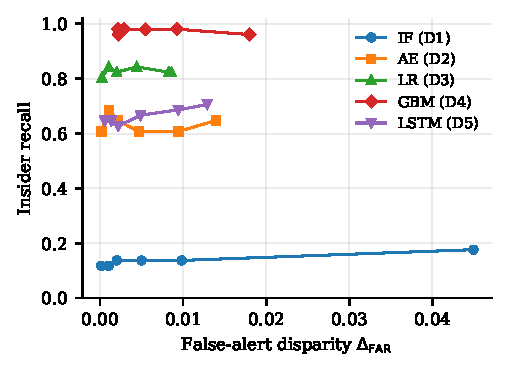
\includegraphics[width=0.95\columnwidth]{figures/pareto.pdf}
\caption{Insider recall versus false-alert disparity of label-free FAIR-IRS as the tolerance $\delta$ varies from $1$ (global top-$k$, rightmost point of each curve) to $0$ (r4.2, functional units).}
\label{fig:s-pareto}
\end{figure}

\begin{table}[!t]
\caption{Both Modes for All Groupings (r4.2, $\delta$ = 0.002)\label{tab:s-modes-grp}}
\centering
\resizebox{\columnwidth}{!}{%
\begin{tabular}{lccccccc}
\toprule
Detector & Grouping & $\Delta_{\mathrm{FAR}}$ B0 & $\Delta_{\mathrm{FAR}}$ B4 & $\Delta_{\mathrm{FAR}}$ B4c & Detected B0 & Detected B4 & Detected B4c \\
\midrule
IF & Func. unit & 0.0449 & 0.0020 & 0.0020 & 9 & 7 & 7 \\
AE & Func. unit & 0.0139 & 0.0021 & 0.0020 & 33 & 33 & 33 \\
LR & Func. unit & 0.0086 & 0.0020 & 0.0019 & 42 & 42 & 43 \\
GBM & Func. unit & 0.0180 & 0.0029 & 0.0020 & 49 & 50 & 49 \\
LSTM & Func. unit & 0.0129 & 0.0022 & 0.0020 & 36 & 32 & 34 \\
IF & Department & 0.0773 & 0.0020 & 0.0020 & 9 & 6 & 7 \\
AE & Department & 0.0252 & 0.0024 & 0.0020 & 33 & 32 & 33 \\
LR & Department & 0.0150 & 0.0033 & 0.0021 & 42 & 38 & 40 \\
GBM & Department & 0.0179 & 0.0044 & 0.0020 & 49 & 48 & 47 \\
LSTM & Department & 0.0192 & 0.0023 & 0.0020 & 36 & 34 & 31 \\
IF & Role & 0.1405 & 0.0027 & 0.0021 & 9 & 4 & 5 \\
AE & Role & 0.0455 & 0.0030 & 0.0020 & 33 & 31 & 27 \\
LR & Role & 0.0293 & 0.0027 & 0.0020 & 42 & 38 & 39 \\
GBM & Role & 0.0313 & 0.0058 & 0.0020 & 49 & 44 & 43 \\
LSTM & Role & 0.0363 & 0.0024 & 0.0020 & 36 & 32 & 30 \\
IF & After-hours & 0.0075 & 0.0020 & 0.0020 & 9 & 8 & 8 \\
AE & After-hours & 0.0012 & 0.0011 & 0.0010 & 33 & 33 & 33 \\
LR & After-hours & 0.0041 & 0.0017 & 0.0019 & 42 & 40 & 41 \\
GBM & After-hours & 0.0034 & 0.0015 & 0.0019 & 49 & 50 & 50 \\
LSTM & After-hours & 0.0030 & 0.0019 & 0.0019 & 36 & 36 & 36 \\
IF & Exposure & 0.0245 & 0.0019 & 0.0020 & 9 & 11 & 11 \\
AE & Exposure & 0.0177 & 0.0022 & 0.0020 & 33 & 34 & 34 \\
LR & Exposure & 0.0010 & 0.0009 & 0.0009 & 42 & 42 & 42 \\
GBM & Exposure & 0.0029 & 0.0003 & 0.0019 & 49 & 50 & 50 \\
LSTM & Exposure & 0.0115 & 0.0021 & 0.0020 & 36 & 33 & 33 \\
\bottomrule
\end{tabular}}
\end{table}
\begin{table}[!t]
\caption{Both Modes Over Five Seeds, Mean and 95\% CI (r4.2, $\delta$ = 0.002)\label{tab:s-modes-seeds}}
\centering
\resizebox{\columnwidth}{!}{%
\begin{tabular}{lccccccc}
\toprule
Detector & Policy & Runs & Recall & Prec. & Day TPR & $\Delta_{\mathrm{FAR}}$ & $\rho_{\mathrm{FAR}}$ \\
\midrule
IF & B0 global & 5 & 0.176 $\pm$ 0.024 & 0.008 $\pm$ 0.001 & 0.022 $\pm$ 0.003 & 0.044 $\pm$ 0.002 & 30.460 $\pm$ 6.784 \\
IF & B4 label-free & 5 & 0.106 $\pm$ 0.037 & 0.004 $\pm$ 0.001 & 0.011 $\pm$ 0.003 & 0.002 $\pm$ 0.000 & 1.217 $\pm$ 0.003 \\
IF & B4c outcome-aware & 5 & 0.125 $\pm$ 0.013 & 0.005 $\pm$ 0.001 & 0.013 $\pm$ 0.002 & 0.002 $\pm$ 0.000 & 1.213 $\pm$ 0.002 \\
AE & B0 global & 5 & 0.565 $\pm$ 0.153 & 0.030 $\pm$ 0.009 & 0.082 $\pm$ 0.026 & 0.015 $\pm$ 0.002 & 3.736 $\pm$ 0.589 \\
AE & B4 label-free & 5 & 0.573 $\pm$ 0.108 & 0.029 $\pm$ 0.008 & 0.078 $\pm$ 0.023 & 0.002 $\pm$ 0.000 & 1.233 $\pm$ 0.028 \\
AE & B4c outcome-aware & 5 & 0.592 $\pm$ 0.121 & 0.030 $\pm$ 0.008 & 0.082 $\pm$ 0.023 & 0.002 $\pm$ 0.000 & 1.220 $\pm$ 0.009 \\
LR & B0 global & 1 & 0.824 & 0.083 & 0.223 & 0.009 & 3.433 \\
LR & B4 label-free & 1 & 0.824 & 0.083 & 0.223 & 0.002 & 1.252 \\
LR & B4c outcome-aware & 1 & 0.843 & 0.085 & 0.230 & 0.002 & 1.239 \\
GBM & B0 global & 5 & 0.922 $\pm$ 0.096 & 0.241 $\pm$ 0.036 & 0.651 $\pm$ 0.098 & 0.016 $\pm$ 0.004 & 5.510 $\pm$ 1.953 \\
GBM & B4 label-free & 5 & 0.894 $\pm$ 0.112 & 0.222 $\pm$ 0.034 & 0.601 $\pm$ 0.091 & 0.003 $\pm$ 0.000 & 1.381 $\pm$ 0.035 \\
GBM & B4c outcome-aware & 5 & 0.878 $\pm$ 0.112 & 0.239 $\pm$ 0.037 & 0.644 $\pm$ 0.101 & 0.002 $\pm$ 0.000 & 1.297 $\pm$ 0.014 \\
\bottomrule
\end{tabular}}
\end{table}
\begin{table}[!t]
\caption{Alert Policies Compared for All Detectors (r4.2, Functional Units, $\delta$ = 0.002)\label{tab:s-policies}}
\centering
\resizebox{\columnwidth}{!}{%
\begin{tabular}{lccccccc}
\toprule
Detector & Policy & Recall [95\% CI] & Prec. & Day TPR & $\Delta_{\mathrm{FAR}}$ & $\rho_{\mathrm{FAR}}$ & Alerts used \\
\midrule
IF & B0 global & 0.176 [0.10, 0.30] & 0.008 & 0.022 & 0.045 & 29.201 & 1.000 \\
IF & B1 per-day quota & 0.137 [0.07, 0.26] & 0.005 & 0.013 & 0.012 & $\infty$ & 1.000 \\
IF & B4 label-free & 0.137 [0.07, 0.26] & 0.005 & 0.013 & 0.002 & 1.218 & 1.000 \\
IF & B4c outcome-aware & 0.137 [0.07, 0.26] & 0.005 & 0.013 & 0.002 & 1.211 & 1.000 \\
IF & B6 group rank & 0.137 [0.07, 0.26] & 0.005 & 0.013 & 0.024 & 4.524 & 1.000 \\
IF & B7 group thresholds & 0.118 [0.06, 0.23] & 0.005 & 0.013 & 0.005 & 1.763 & 1.018 \\
IF & B8 daily parity & 0.137 [0.07, 0.26] & 0.005 & 0.013 & 0.012 & $\infty$ & 1.000 \\
IF & B9 FA*IR bands & 0.137 [0.07, 0.26] & 0.005 & 0.013 & 0.021 & 8.579 & 1.000 \\
AE & B0 global & 0.647 [0.51, 0.76] & 0.037 & 0.099 & 0.014 & 3.198 & 1.000 \\
AE & B1 per-day quota & 0.627 [0.49, 0.75] & 0.032 & 0.087 & 0.011 & $\infty$ & 1.000 \\
AE & B4 label-free & 0.647 [0.51, 0.76] & 0.035 & 0.096 & 0.002 & 1.245 & 1.000 \\
AE & B4c outcome-aware & 0.647 [0.51, 0.76] & 0.036 & 0.097 & 0.002 & 1.215 & 1.000 \\
AE & B6 group rank & 0.647 [0.51, 0.76] & 0.036 & 0.097 & 0.024 & 4.285 & 1.000 \\
AE & B7 group thresholds & 0.588 [0.45, 0.71] & 0.034 & 0.096 & 0.003 & 1.391 & 1.050 \\
AE & B8 daily parity & 0.627 [0.49, 0.75] & 0.032 & 0.087 & 0.011 & $\infty$ & 1.000 \\
AE & B9 FA*IR bands & 0.647 [0.51, 0.76] & 0.037 & 0.099 & 0.010 & 2.629 & 1.000 \\
LR & B0 global & 0.824 [0.70, 0.90] & 0.083 & 0.223 & 0.009 & 3.433 & 1.000 \\
LR & B1 per-day quota & 0.784 [0.65, 0.88] & 0.077 & 0.208 & 0.011 & $\infty$ & 1.000 \\
LR & B4 label-free & 0.824 [0.70, 0.90] & 0.083 & 0.223 & 0.002 & 1.252 & 1.000 \\
LR & B4c outcome-aware & 0.843 [0.72, 0.92] & 0.085 & 0.230 & 0.002 & 1.239 & 1.000 \\
LR & B6 group rank & 0.824 [0.70, 0.90] & 0.083 & 0.223 & 0.021 & 4.009 & 1.000 \\
LR & B7 group thresholds & 0.804 [0.68, 0.89] & 0.084 & 0.228 & 0.006 & 2.014 & 1.010 \\
LR & B8 daily parity & 0.784 [0.65, 0.88] & 0.077 & 0.208 & 0.011 & $\infty$ & 1.000 \\
LR & B9 FA*IR bands & 0.843 [0.72, 0.92] & 0.084 & 0.227 & 0.009 & 3.553 & 1.000 \\
GBM & B0 global & 0.961 [0.87, 0.99] & 0.257 & 0.693 & 0.018 & 5.375 & 1.000 \\
GBM & B1 per-day quota & 0.922 [0.81, 0.97] & 0.231 & 0.624 & 0.011 & $\infty$ & 1.000 \\
GBM & B4 label-free & 0.980 [0.90, 1.00] & 0.237 & 0.639 & 0.003 & 1.400 & 1.000 \\
GBM & B4c outcome-aware & 0.961 [0.87, 0.99] & 0.257 & 0.695 & 0.002 & 1.306 & 1.000 \\
GBM & B6 group rank & 1.000 [0.93, 1.00] & 0.243 & 0.658 & 0.022 & 5.019 & 1.000 \\
GBM & B7 group thresholds & 1.000 [0.93, 1.00] & 0.238 & 0.753 & 0.019 & 3.733 & 1.170 \\
GBM & B8 daily parity & 0.922 [0.81, 0.97] & 0.231 & 0.624 & 0.011 & $\infty$ & 1.000 \\
GBM & B9 FA*IR bands & 0.980 [0.90, 1.00] & 0.252 & 0.681 & 0.014 & 3.898 & 1.000 \\
LSTM & B0 global & 0.706 [0.57, 0.81] & 0.040 & 0.107 & 0.013 & 3.404 & 1.000 \\
LSTM & B1 per-day quota & 0.647 [0.51, 0.76] & 0.034 & 0.091 & 0.011 & $\infty$ & 1.000 \\
LSTM & B4 label-free & 0.627 [0.49, 0.75] & 0.032 & 0.087 & 0.002 & 1.267 & 1.000 \\
LSTM & B4c outcome-aware & 0.667 [0.53, 0.78] & 0.036 & 0.097 & 0.002 & 1.237 & 1.000 \\
LSTM & B6 group rank & 0.627 [0.49, 0.75] & 0.035 & 0.096 & 0.026 & 4.813 & 1.000 \\
LSTM & B7 group thresholds & 0.529 [0.40, 0.66] & 0.034 & 0.091 & 0.005 & 1.739 & 0.996 \\
LSTM & B8 daily parity & 0.647 [0.51, 0.76] & 0.034 & 0.091 & 0.011 & $\infty$ & 1.000 \\
LSTM & B9 FA*IR bands & 0.686 [0.55, 0.80] & 0.038 & 0.102 & 0.011 & 2.924 & 1.000 \\
\bottomrule
\end{tabular}}
\end{table}

\emph{Paired comparison with the global policy.} Table~\ref{tab:s-paired} compares each policy with the global policy on the same insiders in the main run. No single-run difference is significant (exact McNemar $p\ge0.11$): FAIR-IRS allocation loses at most five insiders and gains up to two, while scheduling gains seven or eight insiders for IF and four to six for AE. Over five seeds (Table~\ref{tab:s-paired-pooled}), the losses nevertheless go one way. The label-free mode loses $39$ insider detections and gains $16$, and the outcome-aware mode loses $33$ and gains $17$; IF loses in every seed. Because the seeds share the same insiders, these pooled counts are not independent and the sign-test $p$-values are descriptive.

\emph{Non-inferiority.} Table~\ref{tab:s-noninf} replaces these descriptive counts with a non-inferiority analysis, for three budgets and with the LSTM retrained with four additional seeds. With a margin of $0.05$, non-inferiority holds at $b=1\%$ for AE and LR in both modes and fails for IF, GBM and the LSTM, whose per-run losses are $1.4$ to $3.6$ insiders. At $b=2\%$ it holds for AE, GBM and the LSTM, and at $b=0.5\%$ only for AE in the outcome-aware mode. Outcome-aware scheduling is non-inferior for IF, AE and LR, and superior for IF and AE, but not non-inferior for GBM and the LSTM.

\emph{Insiders removed after confirmation.} In the main runs, a detected insider remains in the population and can be alerted again on later malicious days, which inflates precision and consumes budget. Table~\ref{tab:s-removal} removes each insider the day after their first confirmed alert. GBM's precision under the global policy falls from $0.257$ to $0.045$, so about a fifth of its budget went to known insiders; the freed budget detects two more insiders under the global policy and leaves the parity rules within one insider of their main runs. The disparities and their reduction are unchanged (GBM: $\Delta_{\FAR}=0.020$ under the global policy, $0.0018$ and $0.0020$ under the two modes), and the maximum individual burden rises, because the freed alerts go to benign employees.

\begin{table}[!t]
\caption{Non-Inferiority of Detection Against the Global Policy, Pooled Over Seeds (r4.2, $\delta$ = 0.2 $\times$ Budget). Per-Insider Detection Is Averaged Over Runs and Resampled Over Insiders; ``Per Run'' Is the Mean Change in Insiders Detected; Non-Inferior (NI) if the One-Sided 95\% Lower Bound Exceeds $-0.05$\label{tab:s-noninf}}
\centering
\resizebox{\columnwidth}{!}{%
\begin{tabular}{lccccccccc}
\toprule
Budget & Detector & Policy & Runs & Recall B0 & Recall & Diff. [95\% CI] & Per run & One-sided & NI \\
\midrule
0.5\% & IF & B4 LF & 5 & 0.137 & 0.090 & -0.047 [-0.13, +0.02] & -2.4 & -0.110 & no \\
0.5\% & IF & B4c OA & 5 & 0.137 & 0.106 & -0.031 [-0.10, +0.04] & -1.6 & -0.086 & no \\
0.5\% & AE & B4 LF & 5 & 0.455 & 0.443 & -0.012 [-0.07, +0.04] & -0.6 & -0.055 & no \\
0.5\% & AE & B4c OA & 5 & 0.455 & 0.451 & -0.004 [-0.04, +0.04] & -0.2 & -0.035 & yes \\
0.5\% & LR & B4 LF & 1 & 0.706 & 0.647 & -0.059 [-0.14, +0.02] & -3.0 & -0.137 & no \\
0.5\% & LR & B4c OA & 1 & 0.706 & 0.667 & -0.039 [-0.14, +0.06] & -2.0 & -0.118 & no \\
0.5\% & GBM & B4 LF & 5 & 0.875 & 0.808 & -0.067 [-0.14, -0.00] & -3.4 & -0.125 & no \\
0.5\% & GBM & B4c OA & 5 & 0.875 & 0.804 & -0.071 [-0.15, +0.00] & -3.6 & -0.137 & no \\
0.5\% & LSTM & B4 LF & 5 & 0.565 & 0.537 & -0.027 [-0.11, +0.05] & -1.4 & -0.098 & no \\
0.5\% & LSTM & B4c OA & 5 & 0.565 & 0.518 & -0.047 [-0.12, +0.02] & -2.4 & -0.110 & no \\
1\% & IF & B4 LF & 5 & 0.176 & 0.106 & -0.071 [-0.13, -0.02] & -3.6 & -0.122 & no \\
1\% & IF & B4c OA & 5 & 0.176 & 0.125 & -0.051 [-0.11, -0.01] & -2.6 & -0.098 & no \\
1\% & IF & B5c OA + sched. & 5 & 0.176 & 0.278 & +0.102 [+0.00, +0.20] & +5.2 & +0.020 & yes \\
1\% & AE & B4 LF & 5 & 0.565 & 0.573 & +0.008 [-0.04, +0.05] & +0.4 & -0.027 & yes \\
1\% & AE & B4c OA & 5 & 0.565 & 0.592 & +0.027 [-0.02, +0.08] & +1.4 & -0.012 & yes \\
1\% & AE & B5c OA + sched. & 5 & 0.565 & 0.651 & +0.086 [+0.03, +0.15] & +4.4 & +0.039 & yes \\
1\% & LR & B4 LF & 1 & 0.824 & 0.824 & +0.000 [-0.06, +0.06] & +0.0 & -0.039 & yes \\
1\% & LR & B4c OA & 1 & 0.824 & 0.843 & +0.020 [+0.00, +0.06] & +1.0 & +0.000 & yes \\
1\% & LR & B5c OA + sched. & 1 & 0.824 & 0.863 & +0.039 [-0.04, +0.12] & +2.0 & -0.020 & yes \\
1\% & GBM & B4 LF & 5 & 0.922 & 0.894 & -0.027 [-0.09, +0.02] & -1.4 & -0.071 & no \\
1\% & GBM & B4c OA & 5 & 0.922 & 0.878 & -0.043 [-0.10, +0.00] & -2.2 & -0.090 & no \\
1\% & GBM & B5c OA + sched. & 5 & 0.922 & 0.898 & -0.024 [-0.08, +0.03] & -1.2 & -0.071 & no \\
1\% & LSTM & B4 LF & 5 & 0.694 & 0.647 & -0.047 [-0.13, +0.04] & -2.4 & -0.118 & no \\
1\% & LSTM & B4c OA & 5 & 0.694 & 0.635 & -0.059 [-0.15, +0.02] & -3.0 & -0.129 & no \\
1\% & LSTM & B5c OA + sched. & 5 & 0.694 & 0.682 & -0.012 [-0.09, +0.07] & -0.6 & -0.082 & no \\
2\% & IF & B4 LF & 5 & 0.247 & 0.220 & -0.027 [-0.11, +0.05] & -1.4 & -0.102 & no \\
2\% & IF & B4c OA & 5 & 0.247 & 0.224 & -0.024 [-0.11, +0.06] & -1.2 & -0.098 & no \\
2\% & AE & B4 LF & 5 & 0.722 & 0.769 & +0.047 [-0.01, +0.10] & +2.4 & -0.000 & yes \\
2\% & AE & B4c OA & 5 & 0.722 & 0.753 & +0.031 [-0.02, +0.08] & +1.6 & -0.016 & yes \\
2\% & LR & B4 LF & 1 & 0.882 & 0.863 & -0.020 [-0.06, +0.00] & -1.0 & -0.059 & no \\
2\% & LR & B4c OA & 1 & 0.882 & 0.863 & -0.020 [-0.06, +0.00] & -1.0 & -0.059 & no \\
2\% & GBM & B4 LF & 5 & 0.949 & 0.949 & +0.000 [-0.02, +0.02] & +0.0 & -0.020 & yes \\
2\% & GBM & B4c OA & 5 & 0.949 & 0.941 & -0.008 [-0.05, +0.02] & -0.4 & -0.043 & yes \\
2\% & LSTM & B4 LF & 5 & 0.737 & 0.784 & +0.047 [-0.04, +0.14] & +2.4 & -0.031 & yes \\
2\% & LSTM & B4c OA & 5 & 0.737 & 0.780 & +0.043 [-0.02, +0.11] & +2.2 & -0.012 & yes \\
\bottomrule
\end{tabular}}
\end{table}
\begin{table}[!t]
\caption{Insiders Removed From the Population After Their First Confirmed Alert (r4.2, Functional Units, $\delta$ = 0.002). Alerted: Benign Employees Alerted at Least Once\label{tab:s-removal}}
\centering
\resizebox{\columnwidth}{!}{%
\begin{tabular}{lccccccccc}
\toprule
Detector & Policy & Removed & Det. & Prec. & $\Delta_{\mathrm{FAR}}$ & $\rho_{\mathrm{FAR}}$ & Gini($F$) & $\max F_i$ & Alerted \\
\midrule
IF & B0 global & no & 9 & 0.0081 & 0.0449 & 29.2008 & 0.9803 & 191 & 61 \\
IF & B0 global & yes & 9 & 0.0075 & 0.0450 & 29.2372 & 0.9803 & 191 & 61 \\
IF & B4 LF & no & 7 & 0.0050 & 0.0020 & 1.2183 & 0.9725 & 175 & 71 \\
IF & B4 LF & yes & 7 & 0.0043 & 0.0020 & 1.2155 & 0.9727 & 176 & 70 \\
IF & B4c OA & no & 7 & 0.0050 & 0.0020 & 1.2107 & 0.9726 & 178 & 68 \\
IF & B4c OA & yes & 7 & 0.0043 & 0.0020 & 1.2123 & 0.9727 & 174 & 67 \\
AE & B0 global & no & 33 & 0.0366 & 0.0139 & 3.1979 & 0.9373 & 65 & 145 \\
AE & B0 global & yes & 33 & 0.0242 & 0.0147 & 3.3113 & 0.9368 & 66 & 148 \\
AE & B4 LF & no & 33 & 0.0354 & 0.0021 & 1.2450 & 0.9317 & 65 & 162 \\
AE & B4 LF & yes & 33 & 0.0230 & 0.0021 & 1.2291 & 0.9321 & 64 & 162 \\
AE & B4c OA & no & 33 & 0.0360 & 0.0020 & 1.2153 & 0.9321 & 64 & 161 \\
AE & B4c OA & yes & 32 & 0.0236 & 0.0020 & 1.2195 & 0.9326 & 65 & 158 \\
LR & B0 global & no & 42 & 0.0826 & 0.0086 & 3.4332 & 0.9706 & 168 & 112 \\
LR & B0 global & yes & 42 & 0.0286 & 0.0088 & 3.0609 & 0.9682 & 171 & 118 \\
LR & B4 LF & no & 42 & 0.0826 & 0.0020 & 1.2518 & 0.9672 & 173 & 116 \\
LR & B4 LF & yes & 43 & 0.0280 & 0.0019 & 1.2168 & 0.9650 & 173 & 118 \\
LR & B4c OA & no & 43 & 0.0851 & 0.0019 & 1.2391 & 0.9690 & 169 & 110 \\
LR & B4c OA & yes & 43 & 0.0286 & 0.0019 & 1.2083 & 0.9658 & 172 & 119 \\
GBM & B0 global & no & 49 & 0.2565 & 0.0180 & 5.3753 & 0.9484 & 110 & 148 \\
GBM & B0 global & yes & 51 & 0.0453 & 0.0200 & 4.4345 & 0.9420 & 125 & 166 \\
GBM & B4 LF & no & 50 & 0.2366 & 0.0029 & 1.3997 & 0.9413 & 61 & 152 \\
GBM & B4 LF & yes & 49 & 0.0429 & 0.0018 & 1.2052 & 0.9344 & 72 & 176 \\
GBM & B4c OA & no & 49 & 0.2571 & 0.0020 & 1.3062 & 0.9389 & 60 & 158 \\
GBM & B4c OA & yes & 50 & 0.0441 & 0.0020 & 1.2275 & 0.9355 & 73 & 171 \\
LSTM & B0 global & no & 36 & 0.0398 & 0.0129 & 3.4038 & 0.9091 & 58 & 190 \\
LSTM & B0 global & yes & 36 & 0.0261 & 0.0133 & 3.4947 & 0.9091 & 59 & 190 \\
LSTM & B4 LF & no & 32 & 0.0323 & 0.0022 & 1.2671 & 0.9082 & 49 & 188 \\
LSTM & B4 LF & yes & 31 & 0.0205 & 0.0021 & 1.2458 & 0.9078 & 49 & 187 \\
LSTM & B4c OA & no & 34 & 0.0360 & 0.0020 & 1.2371 & 0.9087 & 49 & 184 \\
LSTM & B4c OA & yes & 33 & 0.0230 & 0.0020 & 1.2300 & 0.9093 & 49 & 184 \\
\bottomrule
\end{tabular}}
\end{table}

\emph{Online dual prices.} Table~\ref{tab:s-dual} compares FAIR-IRS with an online dual-price baseline (B10), which also uses cumulative history. With a large step ($\eta=10$, proportional form), B10 matches FAIR-IRS for every detector: GBM reaches $\Delta_{\FAR}=0.0027$ with $50$ insiders and the LSTM $0.0018$ with $36$. With smaller steps, it leaves the disparity at several times the target (IF: $0.038$ at $\eta=0.1$, $19$ times the target), and the dual-ascent form reaches the target only at a cost of up to $12$ insiders for the LSTM ($36\to24$) and $9$ for AE and GBM. The value of $\eta$ that works was chosen on the test period, which an organization cannot do. What matters is memory, which both methods have and which B1, B8 and B9 lack; FAIR-IRS adds a tolerance fixed in advance and exact optimality in each window.

\begin{table}[!t]
\caption{Paired Comparison of Insider Detection With the Global Policy (r4.2, Main Run): Insiders Lost and Gained, Recall Difference With Paired Bootstrap Interval, and Exact McNemar Test\label{tab:s-paired}}
\centering
\resizebox{\columnwidth}{!}{%
\begin{tabular}{lccccccc}
\toprule
Detector & Policy & Recall B0 & Recall & Difference [95\% CI] & Lost & Gained & McNemar $p$ \\
\midrule
IF & B4 label-free & 0.176 & 0.137 & -0.039 [-0.10, +0.00] & 2 & 0 & 0.50 \\
IF & B4c outcome-aware & 0.176 & 0.137 & -0.039 [-0.10, +0.00] & 2 & 0 & 0.50 \\
IF & B5 label-free + scheduling & 0.176 & 0.294 & +0.118 [+0.00, +0.24] & 2 & 8 & 0.11 \\
IF & B5c outcome-aware + scheduling & 0.176 & 0.275 & +0.098 [+0.00, +0.22] & 2 & 7 & 0.18 \\
IF & B4 label-free, floor 2 & 0.176 & 0.137 & -0.039 [-0.10, +0.00] & 2 & 0 & 0.50 \\
AE & B4 label-free & 0.647 & 0.647 & +0.000 [-0.10, +0.10] & 3 & 3 & 1.00 \\
AE & B4c outcome-aware & 0.647 & 0.647 & +0.000 [-0.06, +0.06] & 1 & 1 & 1.00 \\
AE & B5 label-free + scheduling & 0.647 & 0.745 & +0.098 [+0.00, +0.20] & 1 & 6 & 0.12 \\
AE & B5c outcome-aware + scheduling & 0.647 & 0.725 & +0.078 [+0.02, +0.16] & 0 & 4 & 0.12 \\
AE & B4 label-free, floor 2 & 0.647 & 0.608 & -0.039 [-0.10, +0.00] & 2 & 0 & 0.50 \\
LR & B4 label-free & 0.824 & 0.824 & +0.000 [-0.06, +0.06] & 1 & 1 & 1.00 \\
LR & B4c outcome-aware & 0.824 & 0.843 & +0.020 [+0.00, +0.06] & 0 & 1 & 1.00 \\
LR & B5 label-free + scheduling & 0.824 & 0.843 & +0.020 [-0.04, +0.10] & 1 & 2 & 1.00 \\
LR & B5c outcome-aware + scheduling & 0.824 & 0.863 & +0.039 [-0.04, +0.12] & 1 & 3 & 0.62 \\
LR & B4 label-free, floor 2 & 0.824 & 0.804 & -0.020 [-0.08, +0.04] & 2 & 1 & 1.00 \\
GBM & B4 label-free & 0.961 & 0.980 & +0.020 [-0.04, +0.10] & 1 & 2 & 1.00 \\
GBM & B4c outcome-aware & 0.961 & 0.961 & +0.000 [-0.06, +0.06] & 1 & 1 & 1.00 \\
GBM & B5 label-free + scheduling & 0.961 & 0.980 & +0.020 [-0.04, +0.10] & 1 & 2 & 1.00 \\
GBM & B5c outcome-aware + scheduling & 0.961 & 0.980 & +0.020 [-0.04, +0.10] & 1 & 2 & 1.00 \\
GBM & B4 label-free, floor 2 & 0.961 & 1.000 & +0.039 [+0.00, +0.10] & 0 & 2 & 0.50 \\
LSTM & B4 label-free & 0.706 & 0.627 & -0.078 [-0.18, +0.00] & 5 & 1 & 0.22 \\
LSTM & B4c outcome-aware & 0.706 & 0.667 & -0.039 [-0.14, +0.06] & 4 & 2 & 0.69 \\
LSTM & B5 label-free + scheduling & 0.706 & 0.667 & -0.039 [-0.14, +0.06] & 4 & 2 & 0.69 \\
LSTM & B5c outcome-aware + scheduling & 0.706 & 0.706 & +0.000 [-0.10, +0.10] & 3 & 3 & 1.00 \\
LSTM & B4 label-free, floor 2 & 0.706 & 0.627 & -0.078 [-0.18, +0.00] & 5 & 1 & 0.22 \\
\bottomrule
\end{tabular}}
\end{table}
\begin{table}[!t]
\caption{Paired Comparison Pooled Over Five Seeds (r4.2; Descriptive, Since the Seeds Share the Same Insiders)\label{tab:s-paired-pooled}}
\centering
\resizebox{\columnwidth}{!}{%
\begin{tabular}{lcccccccc}
\toprule
Detector & Policy & Runs & Mean diff. & Min & Max & Lost & Gained & Sign test $p$ \\
\midrule
IF & B4 label-free & 5 & -0.071 & -0.098 & -0.039 & 18 & 0 & 0.000 \\
AE & B4 label-free & 5 & 0.008 & -0.059 & 0.059 & 9 & 11 & 0.824 \\
LR & B4 label-free & 1 & 0.000 & 0.000 & 0.000 & 1 & 1 & 1.000 \\
GBM & B4 label-free & 5 & -0.027 & -0.059 & 0.020 & 11 & 4 & 0.118 \\
all detectors & B4 label-free & 16 & -0.028 & -0.098 & 0.059 & 39 & 16 & 0.003 \\
IF & B4c outcome-aware & 5 & -0.051 & -0.078 & -0.039 & 13 & 0 & 0.000 \\
AE & B4c outcome-aware & 5 & 0.027 & -0.020 & 0.059 & 7 & 14 & 0.189 \\
LR & B4c outcome-aware & 1 & 0.020 & 0.020 & 0.020 & 0 & 1 & 1.000 \\
GBM & B4c outcome-aware & 5 & -0.043 & -0.078 & 0.000 & 13 & 2 & 0.007 \\
all detectors & B4c outcome-aware & 16 & -0.020 & -0.078 & 0.059 & 33 & 17 & 0.033 \\
\bottomrule
\end{tabular}}
\end{table}
\begin{table}[!t]
\caption{Online Dual-Price Baseline (B10, Label-Free Rates) Versus FAIR-IRS (r4.2, Functional Units, $\delta$ = 0.002). The Step Size $\eta$ Is Chosen on the Test Period, Which Favors the Baseline\label{tab:s-dual}}
\centering
\resizebox{\columnwidth}{!}{%
\begin{tabular}{lcccccccc}
\toprule
Detector & Policy & $\eta$ & Detected & Prec. & $\Delta_{\mathrm{AR}}$ & $\Delta_{\mathrm{FAR}}$ & $\rho_{\mathrm{FAR}}$ & $\max F_i$ \\
\midrule
IF & B0 global & -- & 9 & 0.0081 & 0.0454 & 0.0449 & 29.2008 & 191 \\
IF & B4 label-free & -- & 7 & 0.0050 & 0.0020 & 0.0020 & 1.2183 & 175 \\
IF & B10 proportional & 0.1 & 8 & 0.0075 & 0.0384 & 0.0380 & 13.6188 & 192 \\
IF & B10 proportional & 1 & 8 & 0.0068 & 0.0153 & 0.0150 & 3.0903 & 167 \\
IF & B10 proportional & 10 & 7 & 0.0050 & 0.0022 & 0.0020 & 1.2013 & 149 \\
IF & B10 dual ascent & 0.3 & 6 & 0.0050 & 0.0011 & 0.0008 & 1.0808 & 153 \\
IF & B10 dual ascent & 3 & 8 & 0.0050 & 0.0023 & 0.0024 & 1.2554 & 133 \\
IF & B4c outcome-aware & -- & 7 & 0.0050 & 0.0021 & 0.0020 & 1.2107 & 178 \\
AE & B0 global & -- & 33 & 0.0366 & 0.0146 & 0.0139 & 3.1979 & 65 \\
AE & B4 label-free & -- & 33 & 0.0354 & 0.0020 & 0.0021 & 1.2450 & 65 \\
AE & B10 proportional & 0.1 & 33 & 0.0366 & 0.0135 & 0.0128 & 2.9596 & 65 \\
AE & B10 proportional & 1 & 33 & 0.0342 & 0.0062 & 0.0058 & 1.7168 & 61 \\
AE & B10 proportional & 10 & 34 & 0.0329 & 0.0009 & 0.0007 & 1.0741 & 66 \\
AE & B10 dual ascent & 0.3 & 35 & 0.0342 & 0.0017 & 0.0021 & 1.2188 & 63 \\
AE & B10 dual ascent & 3 & 24 & 0.0242 & 0.0015 & 0.0016 & 1.1736 & 56 \\
AE & B4c outcome-aware & -- & 33 & 0.0360 & 0.0024 & 0.0020 & 1.2153 & 64 \\
LR & B0 global & -- & 42 & 0.0826 & 0.0096 & 0.0086 & 3.4332 & 168 \\
LR & B4 label-free & -- & 42 & 0.0826 & 0.0020 & 0.0020 & 1.2518 & 173 \\
LR & B10 proportional & 0.1 & 43 & 0.0839 & 0.0082 & 0.0074 & 2.7499 & 167 \\
LR & B10 proportional & 1 & 43 & 0.0820 & 0.0050 & 0.0043 & 1.6712 & 171 \\
LR & B10 proportional & 10 & 42 & 0.0783 & 0.0008 & 0.0008 & 1.0866 & 170 \\
LR & B10 dual ascent & 0.3 & 40 & 0.0913 & 0.0016 & 0.0019 & 1.2237 & 174 \\
LR & B10 dual ascent & 3 & 42 & 0.0689 & 0.0022 & 0.0024 & 1.2663 & 152 \\
LR & B4c outcome-aware & -- & 43 & 0.0851 & 0.0021 & 0.0019 & 1.2391 & 169 \\
GBM & B0 global & -- & 49 & 0.2565 & 0.0220 & 0.0180 & 5.3753 & 110 \\
GBM & B4 label-free & -- & 50 & 0.2366 & 0.0020 & 0.0029 & 1.3997 & 61 \\
GBM & B10 proportional & 0.1 & 51 & 0.2571 & 0.0168 & 0.0135 & 3.9787 & 91 \\
GBM & B10 proportional & 1 & 51 & 0.2478 & 0.0067 & 0.0063 & 2.0433 & 70 \\
GBM & B10 proportional & 10 & 50 & 0.2292 & 0.0017 & 0.0027 & 1.3621 & 59 \\
GBM & B10 dual ascent & 0.3 & 44 & 0.1944 & 0.0026 & 0.0037 & 1.5406 & 57 \\
GBM & B10 dual ascent & 3 & 40 & 0.1870 & 0.0009 & 0.0019 & 1.2551 & 49 \\
GBM & B4c outcome-aware & -- & 49 & 0.2571 & 0.0039 & 0.0020 & 1.3062 & 60 \\
LSTM & B0 global & -- & 36 & 0.0398 & 0.0137 & 0.0129 & 3.4038 & 58 \\
LSTM & B4 label-free & -- & 32 & 0.0323 & 0.0020 & 0.0022 & 1.2671 & 49 \\
LSTM & B10 proportional & 0.1 & 36 & 0.0379 & 0.0124 & 0.0116 & 3.0791 & 57 \\
LSTM & B10 proportional & 1 & 36 & 0.0366 & 0.0075 & 0.0069 & 2.0441 & 49 \\
LSTM & B10 proportional & 10 & 36 & 0.0342 & 0.0022 & 0.0018 & 1.2040 & 49 \\
LSTM & B10 dual ascent & 0.3 & 29 & 0.0317 & 0.0013 & 0.0015 & 1.1615 & 49 \\
LSTM & B10 dual ascent & 3 & 24 & 0.0211 & 0.0037 & 0.0039 & 1.4671 & 48 \\
LSTM & B4c outcome-aware & -- & 34 & 0.0360 & 0.0023 & 0.0020 & 1.2371 & 49 \\
\bottomrule
\end{tabular}}
\end{table}

\subsection{Memory, Fairness-Aware Baselines and the Guarantee Over Time}
Table~\ref{tab:s-baselines} compares cumulative allocation with two baselines without memory: the same parity rule applied to each day alone (B8) and FA*IR-style binomial bands adapted to several groups (B9). B8 is infeasible on every day, because the share of small groups rounds to zero, and falls back to deficit apportionment on all $251$ days, which leaves some group without alerts ($\rho_{\FAR}=\infty$). B9 keeps detection but reduces disparity only partly. Table~\ref{tab:s-overtime} reports, for each detector and policy, the largest cumulative disparity of the constrained rate after a 30-day burn-in, the share of days on which it exceeded $\delta$, the largest excess, the number of fallback days, and the largest true false-alert disparity after the burn-in. Fig.~\ref{fig:s-traj} shows the trajectories for GBM. Without a floor, both modes stay at or below $\delta$ after the burn-in, up to an excess of at most $0.0004$ in the outcome-aware mode, which comes from verdicts that revise the history after the allocation; score floors break this guarantee.

\begin{table}[!t]
\caption{Fairness-Aware Baselines Without Memory Versus Cumulative Allocation (r4.2, Functional Units, $\delta$ = 0.002)\label{tab:s-baselines}}
\centering
\resizebox{\columnwidth}{!}{%
\begin{tabular}{lcccccccccc}
\toprule
Detector & Policy & Detected & Prec. & Day TPR & $\Delta_{\mathrm{AR}}$ & $\Delta_{\mathrm{FAR}}$ & $\rho_{\mathrm{FAR}}$ & $\max F_i$ & $F_i\ge1$ & Fallback (days) \\
\midrule
IF & B0 global & 9 & 0.008 & 0.022 & 0.045 & 0.045 & 29.201 & 191 & 61 & 0 \\
IF & B8 daily parity & 7 & 0.005 & 0.013 & 0.012 & 0.012 & $\infty$ & 178 & 70 & 251 \\
IF & B9 FA*IR bands & 7 & 0.005 & 0.013 & 0.022 & 0.021 & 8.579 & 202 & 58 & 0 \\
IF & B4 label-free & 7 & 0.005 & 0.013 & 0.002 & 0.002 & 1.218 & 175 & 71 & 7 \\
IF & B4c outcome-aware & 7 & 0.005 & 0.013 & 0.002 & 0.002 & 1.211 & 178 & 68 & 6 \\
AE & B0 global & 33 & 0.037 & 0.099 & 0.015 & 0.014 & 3.198 & 65 & 145 & 0 \\
AE & B8 daily parity & 32 & 0.032 & 0.087 & 0.012 & 0.011 & $\infty$ & 71 & 152 & 251 \\
AE & B9 FA*IR bands & 33 & 0.037 & 0.099 & 0.012 & 0.010 & 2.629 & 70 & 151 & 0 \\
AE & B4 label-free & 33 & 0.035 & 0.096 & 0.002 & 0.002 & 1.245 & 65 & 162 & 7 \\
AE & B4c outcome-aware & 33 & 0.036 & 0.097 & 0.002 & 0.002 & 1.215 & 64 & 161 & 6 \\
LR & B0 global & 42 & 0.083 & 0.223 & 0.010 & 0.009 & 3.433 & 168 & 112 & 0 \\
LR & B8 daily parity & 40 & 0.077 & 0.208 & 0.012 & 0.011 & $\infty$ & 156 & 115 & 251 \\
LR & B9 FA*IR bands & 43 & 0.084 & 0.227 & 0.009 & 0.009 & 3.553 & 170 & 113 & 0 \\
LR & B4 label-free & 42 & 0.083 & 0.223 & 0.002 & 0.002 & 1.252 & 173 & 116 & 7 \\
LR & B4c outcome-aware & 43 & 0.085 & 0.230 & 0.002 & 0.002 & 1.239 & 169 & 110 & 8 \\
GBM & B0 global & 49 & 0.257 & 0.693 & 0.022 & 0.018 & 5.375 & 110 & 148 & 0 \\
GBM & B8 daily parity & 47 & 0.231 & 0.624 & 0.012 & 0.011 & $\infty$ & 77 & 162 & 251 \\
GBM & B9 FA*IR bands & 50 & 0.252 & 0.681 & 0.016 & 0.014 & 3.898 & 101 & 149 & 0 \\
GBM & B4 label-free & 50 & 0.237 & 0.639 & 0.002 & 0.003 & 1.400 & 61 & 152 & 7 \\
GBM & B4c outcome-aware & 49 & 0.257 & 0.695 & 0.004 & 0.002 & 1.306 & 60 & 158 & 8 \\
LSTM & B0 global & 36 & 0.040 & 0.107 & 0.014 & 0.013 & 3.404 & 58 & 190 & 0 \\
LSTM & B8 daily parity & 33 & 0.034 & 0.091 & 0.012 & 0.011 & $\infty$ & 50 & 176 & 251 \\
LSTM & B9 FA*IR bands & 35 & 0.038 & 0.102 & 0.011 & 0.011 & 2.924 & 54 & 190 & 0 \\
LSTM & B4 label-free & 32 & 0.032 & 0.087 & 0.002 & 0.002 & 1.267 & 49 & 188 & 7 \\
LSTM & B4c outcome-aware & 34 & 0.036 & 0.097 & 0.002 & 0.002 & 1.237 & 49 & 184 & 6 \\
\bottomrule
\end{tabular}}
\end{table}
\begin{table}[!t]
\caption{Cumulative Disparity Over the Test Period, After a 30-Day Burn-In (r4.2, $\delta$ = 0.002). Constrained: Disparity of the Rate the Policy Constrains\label{tab:s-overtime}}
\centering
\resizebox{\columnwidth}{!}{%
\begin{tabular}{lccccccccc}
\toprule
Detector & Policy & Constrained & Max disparity & Days $>\delta$ & Max excess & Fallback days & Fallback after day 30 & Max true $\Delta_{\mathrm{FAR}}$ & Alerts used \\
\midrule
IF & B0 global & alert rate & 0.0585 & 1.0000 & 0.0565 & 0 & 0 & 0.0571 & 1.0000 \\
IF & B4 label-free & alert rate & 0.0020 & 0.0000 & 0.0000 & 7 & 0 & 0.0022 & 1.0000 \\
IF & B4c outcome-aware & cleared rate & 0.0020 & 0.0045 & 0.0000 & 6 & 0 & 0.0024 & 1.0000 \\
IF & B4 label-free, floor 2 & alert rate & 0.0045 & 0.5294 & 0.0025 & 23 & 14 & 0.0042 & 0.8727 \\
IF & B4 label-free, floor 1 & alert rate & 0.0036 & 0.9955 & 0.0016 & 82 & 70 & 0.0035 & 0.3211 \\
IF & B4c outcome-aware, floor 2 & cleared rate & 0.0045 & 0.5249 & 0.0025 & 20 & 10 & 0.0043 & 0.8770 \\
IF & B4c outcome-aware, floor 1 & cleared rate & 0.0035 & 0.9955 & 0.0015 & 82 & 70 & 0.0035 & 0.3230 \\
AE & B0 global & alert rate & 0.0177 & 1.0000 & 0.0157 & 0 & 0 & 0.0157 & 1.0000 \\
AE & B4 label-free & alert rate & 0.0020 & 0.0000 & 0.0000 & 7 & 0 & 0.0039 & 1.0000 \\
AE & B4c outcome-aware & cleared rate & 0.0023 & 0.0090 & 0.0003 & 6 & 0 & 0.0021 & 1.0000 \\
AE & B4 label-free, floor 2 & alert rate & 0.0032 & 0.1629 & 0.0012 & 6 & 0 & 0.0027 & 0.9615 \\
AE & B4 label-free, floor 1 & alert rate & 0.0052 & 0.6652 & 0.0032 & 43 & 32 & 0.0045 & 0.7236 \\
AE & B4c outcome-aware, floor 2 & cleared rate & 0.0028 & 0.1493 & 0.0008 & 6 & 0 & 0.0025 & 0.9640 \\
AE & B4c outcome-aware, floor 1 & cleared rate & 0.0050 & 0.7511 & 0.0030 & 54 & 42 & 0.0050 & 0.6932 \\
LR & B0 global & alert rate & 0.0109 & 1.0000 & 0.0089 & 0 & 0 & 0.0098 & 1.0000 \\
LR & B4 label-free & alert rate & 0.0020 & 0.0000 & 0.0000 & 7 & 0 & 0.0055 & 1.0000 \\
LR & B4c outcome-aware & cleared rate & 0.0024 & 0.0090 & 0.0004 & 8 & 0 & 0.0022 & 1.0000 \\
LR & B4 label-free, floor 2 & alert rate & 0.0027 & 0.3348 & 0.0007 & 12 & 6 & 0.0046 & 0.9422 \\
LR & B4 label-free, floor 1 & alert rate & 0.0047 & 0.9955 & 0.0027 & 80 & 70 & 0.0047 & 0.5460 \\
LR & B4c outcome-aware, floor 2 & cleared rate & 0.0029 & 0.3620 & 0.0009 & 10 & 3 & 0.0027 & 0.9385 \\
LR & B4c outcome-aware, floor 1 & cleared rate & 0.0050 & 0.9955 & 0.0030 & 77 & 68 & 0.0050 & 0.5578 \\
GBM & B0 global & alert rate & 0.0508 & 0.9955 & 0.0488 & 0 & 0 & 0.0194 & 1.0000 \\
GBM & B4 label-free & alert rate & 0.0020 & 0.0000 & 0.0000 & 7 & 0 & 0.0065 & 1.0000 \\
GBM & B4c outcome-aware & cleared rate & 0.0021 & 0.1448 & 0.0001 & 8 & 0 & 0.0022 & 1.0000 \\
GBM & B4 label-free, floor 2 & alert rate & 0.0023 & 0.0543 & 0.0003 & 6 & 1 & 0.0070 & 0.9758 \\
GBM & B4 label-free, floor 1 & alert rate & 0.0028 & 0.6968 & 0.0008 & 46 & 34 & 0.0046 & 0.6857 \\
GBM & B4c outcome-aware, floor 2 & cleared rate & 0.0021 & 0.1900 & 0.0001 & 10 & 2 & 0.0022 & 0.9839 \\
GBM & B4c outcome-aware, floor 1 & cleared rate & 0.0023 & 0.7059 & 0.0003 & 34 & 26 & 0.0023 & 0.7677 \\
LSTM & B0 global & alert rate & 0.0220 & 1.0000 & 0.0200 & 0 & 0 & 0.0198 & 1.0000 \\
LSTM & B4 label-free & alert rate & 0.0020 & 0.0000 & 0.0000 & 7 & 0 & 0.0040 & 1.0000 \\
LSTM & B4c outcome-aware & cleared rate & 0.0020 & 0.0090 & 0.0000 & 6 & 0 & 0.0021 & 1.0000 \\
LSTM & B4 label-free, floor 2 & alert rate & 0.0032 & 0.2127 & 0.0012 & 14 & 5 & 0.0038 & 0.9385 \\
LSTM & B4 label-free, floor 1 & alert rate & 0.0040 & 0.8371 & 0.0020 & 58 & 48 & 0.0036 & 0.6901 \\
LSTM & B4c outcome-aware, floor 2 & cleared rate & 0.0032 & 0.2308 & 0.0012 & 12 & 4 & 0.0031 & 0.9311 \\
LSTM & B4c outcome-aware, floor 1 & cleared rate & 0.0033 & 0.8507 & 0.0013 & 53 & 42 & 0.0032 & 0.6857 \\
\bottomrule
\end{tabular}}
\end{table}
\begin{figure}[!t]
\centering
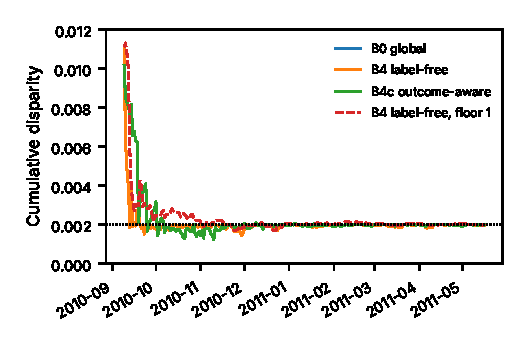
\includegraphics[width=0.95\columnwidth]{figures/trajectory_GBM.pdf}
\caption{Cumulative disparity of the constrained rate over the test period under GBM (r4.2): alert rates for the global policy, label-free FAIR-IRS and label-free FAIR-IRS with floor $\theta=1$, cleared-alert rates for outcome-aware FAIR-IRS. The dotted line is $\delta=0.002$.}
\label{fig:s-traj}
\end{figure}


Table~\ref{tab:s-floor} reports displaced alerts and score floors $\theta$ in the label-free mode, and Table~\ref{tab:s-modes-ext} compares floors and scheduling in both modes. For IF, the floor costs more: with $\theta=1$, only $32\%$ of the budget can be used, because IF's global top-$k$ is concentrated in the administration unit, and $\rho_{\FAR}$ rises to $3.4$. Figs.~\ref{fig:s-lorenzGBM}--\ref{fig:s-lorenzLSTM} show the Lorenz curves of individual burden for GBM, IF and the LSTM. Allocation alone changes them little; scheduling moves them markedly toward the diagonal.

\begin{table}[!t]
\caption{Displaced Alerts and Score Floors for All Evaluated Detectors (r4.2, $\delta$ = 0.002)\label{tab:s-floor}}
\centering
\resizebox{\columnwidth}{!}{%
\begin{tabular}{lcccccccc}
\toprule
Detector & $\theta$ & Recall [CI] & $\Delta_{\mathrm{FAR}}$ & $\rho_{\mathrm{FAR}}$ & Used & Displ. & Rank med. & Rank p90 \\
\midrule
IF & none & 0.137 [0.07, 0.26] & 0.002 & 1.218 & 1.000 & 0.382 & 1.444 & 2.333 \\
IF & 2 & 0.137 [0.07, 0.26] & 0.002 & 1.246 & 0.873 & 0.331 & 1.333 & 1.889 \\
IF & 1.5 & 0.118 [0.06, 0.23] & 0.002 & 1.405 & 0.647 & 0.251 & 1.292 & 1.556 \\
IF & 1 & 0.098 [0.04, 0.21] & 0.003 & 3.361 & 0.321 & 0.000 & -- & -- \\
GBM & none & 0.980 [0.90, 1.00] & 0.003 & 1.400 & 1.000 & 0.174 & 1.333 & 2.000 \\
GBM & 2 & 1.000 [0.93, 1.00] & 0.003 & 1.371 & 0.976 & 0.171 & 1.333 & 1.889 \\
GBM & 1.5 & 0.980 [0.90, 1.00] & 0.003 & 1.406 & 0.944 & 0.160 & 1.222 & 1.556 \\
GBM & 1 & 0.922 [0.81, 0.97] & 0.003 & 1.677 & 0.686 & 0.000 & -- & -- \\
LSTM & none & 0.627 [0.49, 0.75] & 0.002 & 1.267 & 1.000 & 0.141 & 1.444 & 3.000 \\
LSTM & 2 & 0.627 [0.49, 0.75] & 0.002 & 1.296 & 0.939 & 0.122 & 1.333 & 2.000 \\
LSTM & 1.5 & 0.667 [0.53, 0.78] & 0.002 & 1.335 & 0.852 & 0.095 & 1.222 & 1.556 \\
LSTM & 1 & 0.588 [0.45, 0.71] & 0.002 & 1.431 & 0.690 & 0.000 & -- & -- \\
\bottomrule
\end{tabular}}
\end{table}
\begin{table}[!t]
\caption{Score Floors and Scheduling in Both Modes (r4.2, Functional Units, $\delta$ = 0.002)\label{tab:s-modes-ext}}
\centering
\resizebox{\columnwidth}{!}{%
\begin{tabular}{lccccccccc}
\toprule
Detector & Mode & Setting & Recall [95\% CI] & Prec. & $\Delta_{\mathrm{FAR}}$ & $\rho_{\mathrm{FAR}}$ & $\max F_i$ & Alerts used & Displaced \\
\midrule
IF & label-free & $\lambda$ = 0.01 & 0.294 [0.19, 0.43] & 0.011 & 0.002 & 1.192 & 102 & 1.000 & 0.304 \\
IF & outcome-aware & $\lambda$ = 0.01 & 0.275 [0.17, 0.41] & 0.011 & 0.002 & 1.202 & 103 & 1.000 & 0.291 \\
IF & label-free & $\theta$ = 1 & 0.098 [0.04, 0.21] & 0.012 & 0.003 & 3.361 & 83 & 0.321 & 0.000 \\
IF & outcome-aware & $\theta$ = 1 & 0.118 [0.06, 0.23] & 0.013 & 0.003 & 3.389 & 86 & 0.323 & 0.000 \\
IF & label-free & $\theta$ = 2 & 0.137 [0.07, 0.26] & 0.006 & 0.002 & 1.246 & 150 & 0.873 & 0.331 \\
IF & outcome-aware & $\theta$ = 2 & 0.137 [0.07, 0.26] & 0.006 & 0.002 & 1.240 & 152 & 0.877 & 0.336 \\
AE & label-free & $\lambda$ = 0.01 & 0.745 [0.61, 0.84] & 0.042 & 0.002 & 1.250 & 31 & 1.000 & 0.160 \\
AE & outcome-aware & $\lambda$ = 0.01 & 0.725 [0.59, 0.83] & 0.041 & 0.002 & 1.232 & 31 & 1.000 & 0.162 \\
AE & label-free & $\theta$ = 1 & 0.510 [0.38, 0.64] & 0.036 & 0.002 & 1.358 & 44 & 0.724 & 0.000 \\
AE & outcome-aware & $\theta$ = 1 & 0.529 [0.40, 0.66] & 0.039 & 0.002 & 1.341 & 50 & 0.693 & 0.000 \\
AE & label-free & $\theta$ = 2 & 0.608 [0.47, 0.73] & 0.033 & 0.002 & 1.254 & 58 & 0.961 & 0.138 \\
AE & outcome-aware & $\theta$ = 2 & 0.627 [0.49, 0.75] & 0.035 & 0.002 & 1.235 & 61 & 0.964 & 0.139 \\
LR & label-free & $\lambda$ = 0.01 & 0.843 [0.72, 0.92] & 0.103 & 0.002 & 1.192 & 92 & 1.000 & 0.078 \\
LR & outcome-aware & $\lambda$ = 0.01 & 0.863 [0.74, 0.93] & 0.104 & 0.002 & 1.237 & 89 & 1.000 & 0.048 \\
LR & label-free & $\theta$ = 1 & 0.706 [0.57, 0.81] & 0.083 & 0.002 & 1.661 & 111 & 0.546 & 0.000 \\
LR & outcome-aware & $\theta$ = 1 & 0.686 [0.55, 0.80] & 0.082 & 0.002 & 1.804 & 118 & 0.558 & 0.000 \\
LR & label-free & $\theta$ = 2 & 0.804 [0.68, 0.89] & 0.083 & 0.002 & 1.237 & 163 & 0.942 & 0.086 \\
LR & outcome-aware & $\theta$ = 2 & 0.824 [0.70, 0.90] & 0.085 & 0.002 & 1.266 & 152 & 0.939 & 0.077 \\
GBM & label-free & $\lambda$ = 0.01 & 0.980 [0.90, 1.00] & 0.238 & 0.003 & 1.371 & 38 & 1.000 & 0.129 \\
GBM & outcome-aware & $\lambda$ = 0.01 & 0.980 [0.90, 1.00] & 0.257 & 0.002 & 1.316 & 38 & 1.000 & 0.084 \\
GBM & label-free & $\theta$ = 1 & 0.922 [0.81, 0.97] & 0.284 & 0.003 & 1.677 & 47 & 0.686 & 0.000 \\
GBM & outcome-aware & $\theta$ = 1 & 0.882 [0.77, 0.94] & 0.311 & 0.002 & 1.498 & 56 & 0.768 & 0.000 \\
GBM & label-free & $\theta$ = 2 & 1.000 [0.93, 1.00] & 0.245 & 0.003 & 1.371 & 61 & 0.976 & 0.171 \\
GBM & outcome-aware & $\theta$ = 2 & 0.941 [0.84, 0.98] & 0.260 & 0.002 & 1.320 & 60 & 0.984 & 0.143 \\
LSTM & label-free & $\lambda$ = 0.01 & 0.667 [0.53, 0.78] & 0.037 & 0.002 & 1.269 & 30 & 1.000 & 0.157 \\
LSTM & outcome-aware & $\lambda$ = 0.01 & 0.706 [0.57, 0.81] & 0.039 & 0.002 & 1.234 & 32 & 1.000 & 0.158 \\
LSTM & label-free & $\theta$ = 1 & 0.588 [0.45, 0.71] & 0.041 & 0.002 & 1.431 & 49 & 0.690 & 0.000 \\
LSTM & outcome-aware & $\theta$ = 1 & 0.569 [0.43, 0.69] & 0.043 & 0.002 & 1.392 & 46 & 0.686 & 0.000 \\
LSTM & label-free & $\theta$ = 2 & 0.627 [0.49, 0.75] & 0.032 & 0.002 & 1.296 & 49 & 0.939 & 0.122 \\
LSTM & outcome-aware & $\theta$ = 2 & 0.627 [0.49, 0.75] & 0.035 & 0.002 & 1.258 & 49 & 0.931 & 0.121 \\
\bottomrule
\end{tabular}}
\end{table}
\begin{figure}[!t]
\centering
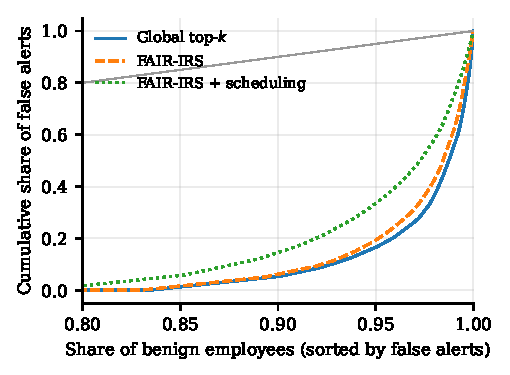
\includegraphics[width=0.95\columnwidth]{figures/lorenz_GBM.pdf}
\caption{Lorenz curves of cleared alerts per benign employee under GBM (r4.2) for the global policy, FAIR-IRS, and FAIR-IRS with scheduling ($\lambda=0.01$). The closer a curve is to the diagonal, the more evenly the burden is shared. The horizontal axis starts at the 80th percentile.}
\label{fig:s-lorenzGBM}
\end{figure}
\begin{figure}[!t]
\centering
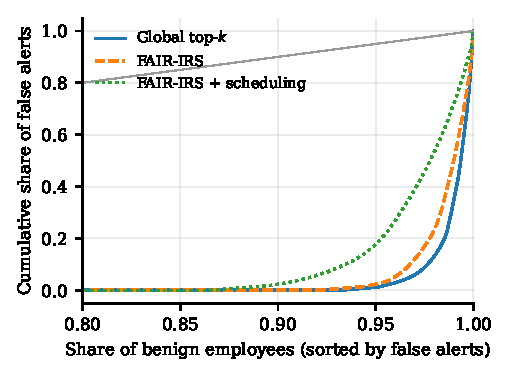
\includegraphics[width=0.95\columnwidth]{figures/lorenz_IF.pdf}
\caption{Lorenz curves of cleared alerts per benign employee under IF (r4.2). The horizontal axis starts at the 80th percentile.}
\label{fig:s-lorenzIF}
\end{figure}
\begin{figure}[!t]
\centering
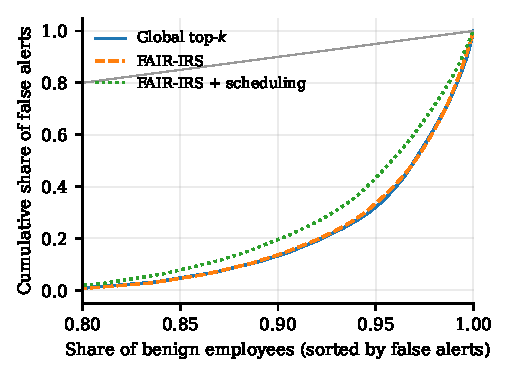
\includegraphics[width=0.95\columnwidth]{figures/lorenz_LSTM.pdf}
\caption{Lorenz curves of cleared alerts per benign employee under the LSTM (r4.2). The horizontal axis starts at the 80th percentile.}
\label{fig:s-lorenzLSTM}
\end{figure}

\emph{Deficit apportionment, histories and monthly disparity.} Table~\ref{tab:s-windows} compares the parity rules and histories, including over rolling windows. Deficit apportionment used alone (B11, B11c) reaches $\Delta_{\FAR}\le0.0006$ for every detector except label-free GBM ($0.0022$), with detection within two insiders of the exact rule, and never falls back, because it has no tolerance to violate. Under cumulative histories, the exact rule's 30-day disparity has a median of $0.0028$ to $0.0054$ and a maximum of $0.0055$ to $0.0147$. Histories limited to $30$ or $90$ days and the discounted history lower the maximum to $0.0036$--$0.0101$, but the 30-day history falls back on $15$ to $43$ days; the discounted history keeps the $5$ to $7$ fallback days of the cumulative one and a 30-day maximum of at most $0.0047$. Dual prices with the tuned step reach a 30-day maximum of $0.0058$ to $0.0102$. The employee-level disparity over calendar months, the quantity of the private reports, is $0.039$ to $0.082$ under the global policy and $0.028$ to $0.060$ under the exact rule: parity on user-day rates reduces it, but does not equalize how many distinct employees of each group are alerted.

\begin{table}[!t]
\caption{Memory-Based Parity Rules and Histories: Detection, Cumulative False-Alert Disparity, Disparity Over Rolling 30- and 90-Day Windows (Median and Maximum Over Windows), Mean Employee-Level Disparity Over Calendar Months, Maximum Individual Burden and Fallback Days (r4.2, Functional Units, $\delta$ = 0.002)\label{tab:s-windows}}
\centering
\resizebox{\columnwidth}{!}{%
\begin{tabular}{lcccccccccc}
\toprule
Detector & Policy & Det. & $\Delta_{\mathrm{FAR}}$ & 30 d med. & 30 d max & 90 d med. & 90 d max & Empl.-month & $\max F_i$ & Fallb. \\
\midrule
IF & B0 global & 9 & 0.0449 & 0.0433 & 0.0589 & 0.0430 & 0.0487 & 0.0588 & 191 & 0 \\
IF & B8 daily parity & 7 & 0.0117 & 0.0121 & 0.0126 & 0.0121 & 0.0125 & 0.0619 & 178 & 251 \\
IF & B9 FA*IR bands & 7 & 0.0215 & 0.0219 & 0.0249 & 0.0219 & 0.0232 & 0.0352 & 202 & 0 \\
IF & B10 dual prices (eta 10), LF & 7 & 0.0020 & 0.0029 & 0.0058 & 0.0021 & 0.0034 & 0.0300 & 149 & 0 \\
IF & B11 deficit apport., LF & 6 & 0.0001 & 0.0007 & 0.0031 & 0.0003 & 0.0010 & 0.0348 & 161 & 0 \\
IF & B11c deficit apport., OA & 7 & 0.0001 & 0.0007 & 0.0019 & 0.0003 & 0.0007 & 0.0387 & 161 & 0 \\
IF & B4 LF & 7 & 0.0020 & 0.0028 & 0.0147 & 0.0022 & 0.0042 & 0.0277 & 175 & 7 \\
IF & B4 LF, 30-day history & 7 & 0.0016 & 0.0020 & 0.0037 & 0.0017 & 0.0023 & 0.0296 & 164 & 30 \\
IF & B4 LF, 90-day history & 7 & 0.0020 & 0.0025 & 0.0058 & 0.0020 & 0.0025 & 0.0275 & 176 & 11 \\
IF & B4c OA & 7 & 0.0020 & 0.0028 & 0.0114 & 0.0022 & 0.0037 & 0.0293 & 178 & 6 \\
IF & B4c OA, 30-day history & 7 & 0.0015 & 0.0020 & 0.0036 & 0.0017 & 0.0022 & 0.0354 & 162 & 33 \\
IF & B4c OA, 90-day history & 7 & 0.0020 & 0.0026 & 0.0054 & 0.0020 & 0.0026 & 0.0353 & 174 & 7 \\
IF & B4c OA, discounted (30 d) & 7 & 0.0018 & 0.0021 & 0.0038 & 0.0019 & 0.0022 & 0.0286 & 173 & 7 \\
AE & B0 global & 33 & 0.0139 & 0.0156 & 0.0229 & 0.0142 & 0.0173 & 0.0674 & 65 & 0 \\
AE & B8 daily parity & 32 & 0.0114 & 0.0112 & 0.0126 & 0.0112 & 0.0123 & 0.1008 & 71 & 251 \\
AE & B9 FA*IR bands & 33 & 0.0104 & 0.0116 & 0.0188 & 0.0110 & 0.0129 & 0.0638 & 70 & 0 \\
AE & B10 dual prices (eta 10), LF & 34 & 0.0007 & 0.0032 & 0.0088 & 0.0015 & 0.0032 & 0.0351 & 66 & 0 \\
AE & B11 deficit apport., LF & 31 & 0.0002 & 0.0010 & 0.0033 & 0.0005 & 0.0011 & 0.0598 & 69 & 0 \\
AE & B11c deficit apport., OA & 33 & 0.0001 & 0.0007 & 0.0022 & 0.0002 & 0.0009 & 0.0446 & 70 & 0 \\
AE & B4 LF & 33 & 0.0021 & 0.0036 & 0.0087 & 0.0022 & 0.0031 & 0.0457 & 65 & 7 \\
AE & B4 LF, 30-day history & 32 & 0.0013 & 0.0022 & 0.0051 & 0.0015 & 0.0026 & 0.0416 & 65 & 22 \\
AE & B4 LF, 90-day history & 33 & 0.0019 & 0.0036 & 0.0068 & 0.0020 & 0.0031 & 0.0431 & 63 & 10 \\
AE & B4c OA & 33 & 0.0020 & 0.0035 & 0.0093 & 0.0022 & 0.0034 & 0.0416 & 64 & 6 \\
AE & B4c OA, 30-day history & 31 & 0.0013 & 0.0019 & 0.0043 & 0.0015 & 0.0021 & 0.0406 & 61 & 26 \\
AE & B4c OA, 90-day history & 34 & 0.0018 & 0.0031 & 0.0059 & 0.0019 & 0.0024 & 0.0390 & 63 & 6 \\
AE & B4c OA, discounted (30 d) & 33 & 0.0016 & 0.0023 & 0.0045 & 0.0018 & 0.0022 & 0.0424 & 70 & 6 \\
LR & B0 global & 42 & 0.0086 & 0.0101 & 0.0152 & 0.0089 & 0.0112 & 0.0388 & 168 & 0 \\
LR & B8 daily parity & 40 & 0.0110 & 0.0113 & 0.0126 & 0.0111 & 0.0120 & 0.0675 & 156 & 251 \\
LR & B9 FA*IR bands & 43 & 0.0086 & 0.0098 & 0.0146 & 0.0086 & 0.0106 & 0.0358 & 170 & 0 \\
LR & B10 dual prices (eta 10), LF & 42 & 0.0008 & 0.0037 & 0.0102 & 0.0014 & 0.0040 & 0.0395 & 170 & 0 \\
LR & B11 deficit apport., LF & 41 & 0.0003 & 0.0015 & 0.0039 & 0.0010 & 0.0018 & 0.0433 & 151 & 0 \\
LR & B11c deficit apport., OA & 44 & 0.0001 & 0.0008 & 0.0021 & 0.0003 & 0.0007 & 0.0693 & 148 & 0 \\
LR & B4 LF & 42 & 0.0020 & 0.0041 & 0.0086 & 0.0028 & 0.0045 & 0.0356 & 173 & 7 \\
LR & B4 LF, 30-day history & 41 & 0.0008 & 0.0023 & 0.0046 & 0.0015 & 0.0023 & 0.0490 & 172 & 15 \\
LR & B4 LF, 90-day history & 42 & 0.0016 & 0.0037 & 0.0086 & 0.0015 & 0.0045 & 0.0361 & 173 & 7 \\
LR & B4c OA & 43 & 0.0019 & 0.0034 & 0.0088 & 0.0029 & 0.0042 & 0.0400 & 169 & 8 \\
LR & B4c OA, 30-day history & 42 & 0.0011 & 0.0018 & 0.0043 & 0.0013 & 0.0025 & 0.0506 & 168 & 18 \\
LR & B4c OA, 90-day history & 43 & 0.0016 & 0.0032 & 0.0060 & 0.0018 & 0.0025 & 0.0395 & 169 & 8 \\
LR & B4c OA, discounted (30 d) & 43 & 0.0014 & 0.0025 & 0.0047 & 0.0016 & 0.0024 & 0.0387 & 170 & 7 \\
GBM & B0 global & 49 & 0.0180 & 0.0187 & 0.0243 & 0.0184 & 0.0213 & 0.0553 & 110 & 0 \\
GBM & B8 daily parity & 47 & 0.0107 & 0.0107 & 0.0126 & 0.0107 & 0.0120 & 0.0807 & 77 & 251 \\
GBM & B9 FA*IR bands & 50 & 0.0141 & 0.0160 & 0.0233 & 0.0170 & 0.0187 & 0.0482 & 101 & 0 \\
GBM & B10 dual prices (eta 10), LF & 50 & 0.0027 & 0.0062 & 0.0089 & 0.0045 & 0.0067 & 0.0427 & 59 & 0 \\
GBM & B11 deficit apport., LF & 49 & 0.0022 & 0.0050 & 0.0087 & 0.0041 & 0.0060 & 0.0484 & 62 & 0 \\
GBM & B11c deficit apport., OA & 49 & 0.0001 & 0.0008 & 0.0022 & 0.0003 & 0.0010 & 0.0411 & 55 & 0 \\
GBM & B4 LF & 50 & 0.0029 & 0.0054 & 0.0091 & 0.0046 & 0.0058 & 0.0430 & 61 & 7 \\
GBM & B4 LF, 30-day history & 49 & 0.0024 & 0.0053 & 0.0084 & 0.0041 & 0.0061 & 0.0488 & 57 & 43 \\
GBM & B4 LF, 90-day history & 49 & 0.0026 & 0.0062 & 0.0101 & 0.0048 & 0.0064 & 0.0404 & 60 & 10 \\
GBM & B4c OA & 49 & 0.0020 & 0.0029 & 0.0055 & 0.0023 & 0.0032 & 0.0423 & 60 & 8 \\
GBM & B4c OA, 30-day history & 48 & 0.0013 & 0.0020 & 0.0042 & 0.0016 & 0.0023 & 0.0357 & 56 & 38 \\
GBM & B4c OA, 90-day history & 47 & 0.0018 & 0.0032 & 0.0064 & 0.0020 & 0.0023 & 0.0424 & 58 & 14 \\
GBM & B4c OA, discounted (30 d) & 50 & 0.0017 & 0.0023 & 0.0044 & 0.0019 & 0.0024 & 0.0401 & 60 & 5 \\
LSTM & B0 global & 36 & 0.0129 & 0.0127 & 0.0212 & 0.0115 & 0.0144 & 0.0822 & 58 & 0 \\
LSTM & B8 daily parity & 33 & 0.0111 & 0.0112 & 0.0126 & 0.0109 & 0.0120 & 0.1043 & 50 & 251 \\
LSTM & B9 FA*IR bands & 35 & 0.0106 & 0.0110 & 0.0169 & 0.0092 & 0.0116 & 0.0733 & 54 & 0 \\
LSTM & B10 dual prices (eta 10), LF & 36 & 0.0018 & 0.0033 & 0.0083 & 0.0017 & 0.0050 & 0.0553 & 49 & 0 \\
LSTM & B11 deficit apport., LF & 33 & 0.0006 & 0.0011 & 0.0031 & 0.0008 & 0.0014 & 0.0518 & 50 & 0 \\
LSTM & B11c deficit apport., OA & 32 & 0.0001 & 0.0006 & 0.0024 & 0.0002 & 0.0007 & 0.0446 & 49 & 0 \\
LSTM & B4 LF & 32 & 0.0022 & 0.0038 & 0.0090 & 0.0025 & 0.0043 & 0.0599 & 49 & 7 \\
LSTM & B4 LF, 30-day history & 34 & 0.0012 & 0.0020 & 0.0052 & 0.0014 & 0.0021 & 0.0491 & 49 & 25 \\
LSTM & B4 LF, 90-day history & 31 & 0.0017 & 0.0032 & 0.0065 & 0.0021 & 0.0028 & 0.0576 & 49 & 8 \\
LSTM & B4c OA & 34 & 0.0020 & 0.0034 & 0.0080 & 0.0022 & 0.0040 & 0.0548 & 49 & 6 \\
LSTM & B4c OA, 30-day history & 33 & 0.0014 & 0.0019 & 0.0039 & 0.0015 & 0.0021 & 0.0504 & 49 & 21 \\
LSTM & B4c OA, 90-day history & 35 & 0.0019 & 0.0035 & 0.0087 & 0.0019 & 0.0024 & 0.0457 & 49 & 7 \\
LSTM & B4c OA, discounted (30 d) & 36 & 0.0017 & 0.0021 & 0.0039 & 0.0017 & 0.0023 & 0.0517 & 49 & 7 \\
\bottomrule
\end{tabular}}
\end{table}

\subsection{Uneven Prevalence}
Table~\ref{tab:s-prev} reports simulation S6 for the three detectors: the smallest (Other, 34 employees) or the largest (R\&D, 316 employees) functional unit receives synthetic insiders until $1$, $2$, $5$ or $10\%$ of its user-days are malicious. Recall is that of the target group's insiders (real insiders when no group is targeted). The label-free mode raises the false-alert disparity of GBM and, to a lesser extent, of the LSTM as prevalence grows, and loses insiders of the target group; IF hardly reacts, because it rarely alerts the synthetic insiders. The outcome-aware mode keeps the disparity close to $\delta$ in every setting. Table~\ref{tab:s-prev-audit} reports the absolute error of the outcome-based audit with correct verdicts and when $30\%$ of the alerts on malicious user-days are wrongly cleared, and the share of draws in which the bound of Proposition~1 holds under analyst error with $\bar\pi=15\%$. With correct verdicts, the error stays below $0.0015$; with analyst error, it reaches $0.013$ for the global policy, and the bound fails in most draws for GBM under FAIR-IRS.

\begin{table}[!t]
\caption{Heterogeneous Prevalence: False-Alert Disparity and Recall of the Target Group's Insiders for All Settings (r4.2, Mean of Three Draws)\label{tab:s-prev}}
\centering
\resizebox{\columnwidth}{!}{%
\begin{tabular}{lcccccccc}
\toprule
Detector & Group & $\pi_g$ & $\Delta_{\mathrm{FAR}}$ B0 & $\Delta_{\mathrm{FAR}}$ B4 & $\Delta_{\mathrm{FAR}}$ B4c & Recall B0 & Recall B4 & Recall B4c \\
\midrule
GBM & none & -- & 0.018 & 0.003 & 0.002 & 0.961 & 0.980 & 0.961 \\
GBM & Other (34) & 1\% & 0.018 & 0.003 & 0.002 & 1.000 & 1.000 & 0.833 \\
GBM & Other (34) & 2\% & 0.018 & 0.003 & 0.002 & 0.939 & 0.909 & 0.765 \\
GBM & Other (34) & 5\% & 0.018 & 0.006 & 0.002 & 0.955 & 0.743 & 0.718 \\
GBM & Other (34) & 10\% & 0.014 & 0.008 & 0.002 & 0.948 & 0.615 & 0.833 \\
GBM & R\&D (316) & 1\% & 0.016 & 0.005 & 0.002 & 0.967 & 0.930 & 0.955 \\
GBM & R\&D (316) & 2\% & 0.012 & 0.008 & 0.002 & 0.925 & 0.850 & 0.927 \\
GBM & R\&D (316) & 5\% & 0.002 & 0.010 & 0.002 & 0.841 & 0.658 & 0.840 \\
GBM & R\&D (316) & 10\% & 0.001 & 0.010 & 0.001 & 0.780 & 0.599 & 0.779 \\
LSTM & none & -- & 0.013 & 0.002 & 0.002 & 0.706 & 0.627 & 0.667 \\
LSTM & Other (34) & 1\% & 0.013 & 0.002 & 0.002 & 0.667 & 0.333 & 0.667 \\
LSTM & Other (34) & 2\% & 0.013 & 0.002 & 0.002 & 0.626 & 0.578 & 0.578 \\
LSTM & Other (34) & 5\% & 0.013 & 0.002 & 0.002 & 0.627 & 0.472 & 0.520 \\
LSTM & Other (34) & 10\% & 0.013 & 0.004 & 0.002 & 0.625 & 0.448 & 0.562 \\
LSTM & R\&D (316) & 1\% & 0.013 & 0.002 & 0.002 & 0.552 & 0.527 & 0.552 \\
LSTM & R\&D (316) & 2\% & 0.012 & 0.002 & 0.002 & 0.528 & 0.524 & 0.524 \\
LSTM & R\&D (316) & 5\% & 0.011 & 0.004 & 0.002 & 0.478 & 0.447 & 0.476 \\
LSTM & R\&D (316) & 10\% & 0.011 & 0.005 & 0.002 & 0.469 & 0.438 & 0.467 \\
IF & none & -- & 0.045 & 0.002 & 0.002 & 0.176 & 0.137 & 0.137 \\
IF & Other (34) & 1\% & 0.045 & 0.002 & 0.002 & 0.000 & 0.000 & 0.000 \\
IF & Other (34) & 2\% & 0.045 & 0.002 & 0.002 & 0.108 & 0.108 & 0.139 \\
IF & Other (34) & 5\% & 0.045 & 0.002 & 0.002 & 0.121 & 0.153 & 0.194 \\
IF & Other (34) & 10\% & 0.045 & 0.002 & 0.002 & 0.198 & 0.208 & 0.229 \\
IF & R\&D (316) & 1\% & 0.045 & 0.002 & 0.002 & 0.174 & 0.171 & 0.174 \\
IF & R\&D (316) & 2\% & 0.045 & 0.002 & 0.002 & 0.217 & 0.221 & 0.219 \\
IF & R\&D (316) & 5\% & 0.045 & 0.002 & 0.003 & 0.207 & 0.217 & 0.217 \\
IF & R\&D (316) & 10\% & 0.045 & 0.002 & 0.003 & 0.204 & 0.212 & 0.211 \\
\bottomrule
\end{tabular}}
\end{table}
\begin{table}[!t]
\caption{Error of the Outcome-Based Audit With Correct Verdicts and With 30\% of Malicious Alerts Wrongly Cleared (``miss''), and Share of Draws in Which the Bound Holds (r4.2)\label{tab:s-prev-audit}}
\centering
\resizebox{\columnwidth}{!}{%
\begin{tabular}{lccccccc}
\toprule
Detector & Group & $\pi_g$ & Error B0 & Error B4 & Error B0, miss & Error B4, miss & Holds B4, miss ($\bar\pi$ = 15\%) \\
\midrule
GBM & none & -- & 0.0002 & 0.0001 & 0.0011 & 0.0003 & 1.0000 \\
GBM & Other (34) & 1\% & 0.0002 & 0.0000 & 0.0013 & 0.0002 & 1.0000 \\
GBM & Other (34) & 2\% & 0.0004 & 0.0000 & 0.0032 & 0.0004 & 1.0000 \\
GBM & Other (34) & 5\% & 0.0010 & 0.0002 & 0.0085 & 0.0020 & 0.3333 \\
GBM & Other (34) & 10\% & 0.0014 & 0.0001 & 0.0129 & 0.0024 & 0.6667 \\
GBM & R\&D (316) & 1\% & 0.0002 & 0.0000 & 0.0011 & 0.0014 & 1.0000 \\
GBM & R\&D (316) & 2\% & 0.0001 & 0.0000 & 0.0011 & 0.0024 & 0.0000 \\
GBM & R\&D (316) & 5\% & 0.0000 & 0.0001 & 0.0054 & 0.0032 & 0.0000 \\
GBM & R\&D (316) & 10\% & 0.0000 & 0.0001 & 0.0065 & 0.0032 & 0.0000 \\
LSTM & none & -- & 0.0000 & 0.0000 & 0.0000 & 0.0001 & 1.0000 \\
LSTM & Other (34) & 1\% & 0.0000 & 0.0000 & 0.0001 & 0.0001 & 1.0000 \\
LSTM & Other (34) & 2\% & 0.0000 & 0.0000 & 0.0001 & 0.0001 & 1.0000 \\
LSTM & Other (34) & 5\% & 0.0000 & 0.0003 & 0.0001 & 0.0001 & 1.0000 \\
LSTM & Other (34) & 10\% & 0.0000 & 0.0005 & 0.0001 & 0.0007 & 1.0000 \\
LSTM & R\&D (316) & 1\% & 0.0000 & 0.0000 & 0.0001 & 0.0001 & 1.0000 \\
LSTM & R\&D (316) & 2\% & 0.0000 & 0.0000 & 0.0001 & 0.0001 & 1.0000 \\
LSTM & R\&D (316) & 5\% & 0.0000 & 0.0003 & 0.0001 & 0.0010 & 1.0000 \\
LSTM & R\&D (316) & 10\% & 0.0000 & 0.0003 & 0.0002 & 0.0013 & 1.0000 \\
IF & none & -- & 0.0001 & 0.0000 & 0.0000 & 0.0000 & 1.0000 \\
IF & Other (34) & 1\% & 0.0001 & 0.0000 & 0.0002 & 0.0000 & 1.0000 \\
IF & Other (34) & 2\% & 0.0000 & 0.0000 & 0.0002 & 0.0000 & 1.0000 \\
IF & Other (34) & 5\% & 0.0000 & 0.0000 & 0.0002 & 0.0000 & 1.0000 \\
IF & Other (34) & 10\% & 0.0000 & 0.0003 & 0.0006 & 0.0001 & 1.0000 \\
IF & R\&D (316) & 1\% & 0.0001 & 0.0001 & 0.0001 & 0.0000 & 1.0000 \\
IF & R\&D (316) & 2\% & 0.0001 & 0.0000 & 0.0001 & 0.0001 & 1.0000 \\
IF & R\&D (316) & 5\% & 0.0001 & 0.0000 & 0.0001 & 0.0001 & 1.0000 \\
IF & R\&D (316) & 10\% & 0.0001 & 0.0000 & 0.0002 & 0.0001 & 1.0000 \\
\bottomrule
\end{tabular}}
\end{table}

\subsection{Realistic Investigation Verdicts}
Table~\ref{tab:s-feedback} reports outcome-aware allocation under simulation S10. Until its verdict is known, an alert counts as cleared, so delays and missing verdicts make the outcome-aware mode closer to the label-free mode. ``Missed'' verdicts clear malicious alerts; ``false confirmation'' confirms benign alerts as malicious; ``smallest'' and ``largest'' restrict the error to the smallest (34 employees) or largest (316) functional unit. The estimate column is the outcome-based audit computed from the recorded verdicts, which is what an oversight body would see. Wrongly confirmed innocents in one group raise the true disparity while the estimate stays at the target.

\begin{table}[!t]
\caption{Outcome-Aware Allocation Under Realistic Investigation Verdicts (r4.2, $\delta$ = 0.002, Mean of Three Draws). Estimate: Outcome-Based Audit From the Recorded Verdicts\label{tab:s-feedback}}
\centering
\resizebox{\columnwidth}{!}{%
\begin{tabular}{lcccccc}
\toprule
Policy / verdicts & $\Delta_{\mathrm{FAR}}$ GBM & $\Delta_{\mathrm{FAR}}$ LSTM & $\Delta_{\mathrm{FAR}}$ IF & Estimate GBM & Detected GBM & Detected LSTM \\
\midrule
B0 global & 0.0180 & 0.0129 & 0.0449 & 0.0178 & 49.0 & 36.0 \\
B4 label-free & 0.0029 & 0.0022 & 0.0020 & 0.0028 & 50.0 & 32.0 \\
correct, immediate & 0.0020 & 0.0020 & 0.0020 & 0.0020 & 49.0 & 34.0 \\
delay 3 days & 0.0020 & 0.0020 & 0.0020 & 0.0020 & 49.0 & 31.0 \\
delay 7 days & 0.0020 & 0.0020 & 0.0020 & 0.0020 & 49.0 & 32.0 \\
delay 14 days & 0.0020 & 0.0020 & 0.0020 & 0.0020 & 50.0 & 33.0 \\
delay 30 days & 0.0020 & 0.0020 & 0.0020 & 0.0020 & 50.0 & 33.0 \\
missing 20\% & 0.0023 & 0.0021 & 0.0020 & 0.0023 & 49.3 & 32.3 \\
missing 50\% & 0.0023 & 0.0021 & 0.0020 & 0.0023 & 48.7 & 33.0 \\
revised after 30 days (30\%) & 0.0020 & 0.0020 & 0.0020 & 0.0020 & 49.3 & 31.7 \\
missed 30\%, all groups & 0.0020 & 0.0020 & 0.0020 & 0.0020 & 49.3 & 32.3 \\
false confirmation 5\%, all groups & 0.0022 & 0.0022 & 0.0022 & 0.0020 & 47.3 & 33.0 \\
missed 30\%, smallest group only & 0.0020 & 0.0020 & 0.0020 & 0.0020 & 49.3 & 34.0 \\
false confirmation 5\%, smallest group only & 0.0022 & 0.0024 & 0.0020 & 0.0020 & 48.7 & 33.3 \\
false confirmation 20\%, smallest group only & 0.0045 & 0.0036 & 0.0031 & 0.0020 & 48.0 & 33.0 \\
missed 30\%, largest group only & 0.0020 & 0.0020 & 0.0020 & 0.0020 & 49.0 & 32.3 \\
false confirmation 5\%, largest group only & 0.0020 & 0.0024 & 0.0025 & 0.0020 & 48.3 & 32.0 \\
false confirmation 20\%, largest group only & 0.0021 & 0.0042 & 0.0046 & 0.0020 & 48.7 & 32.7 \\
delay 7 days + missing 20\% + missed 30\% & 0.0023 & 0.0021 & 0.0020 & 0.0021 & 48.7 & 34.0 \\
\bottomrule
\end{tabular}}
\end{table}

\emph{Re-checking confirmations.} Table~\ref{tab:s-fc} evaluates Corollary~1 when benign alerts are wrongly confirmed at rate $f\in\{0,0.05,0.1,0.2,0.3\}$, in all groups, in the smallest group or in the largest group, for three detectors and three draws ($117$ cases). The plain outcome-based audit reports $0.0019$ to $0.0020$ in every case, because it relies on the same verdicts, while the true disparity under the outcome-aware mode reaches $0.0055$ on average over the three draws and $0.0063$ in a single draw. The bound of Corollary~1, with $f_g$ bounded by re-checking a random $10\%$ of each group's confirmed alerts and taking a $95\%$ Clopper--Pearson upper bound on the error rate, held in all $117$ cases. Its price is conservatism: without errors, it lies between $0.0028$ and $0.0056$, against a true disparity of $0.0020$. Re-checking $20\%$ or $50\%$ of confirmed alerts tightens it: the largest error-free bound falls from $0.0056$ to $0.0048$ and $0.0036$, and the bound still held in all cases.

\emph{Joint errors and a fallible re-checker.} Table~\ref{tab:s-joint} combines false confirmations with $30\%$ missed insiders and a re-checker who overlooks $0$ to $20\%$ of the false confirmations it examines, for GBM, the LSTM and IF ($10\%$ of confirmations re-checked, $20$ re-check samples per draw). Missed insiders count as cleared alerts, which inflates the estimated burden of their groups, including possibly the least-alerted one, and an imperfect re-checker shrinks $\bar q_g$. With per-group $95\%$ Clopper--Pearson bounds, the bound of Corollary~1 held in $97\%$ or more of the samples on average, but in only $65\%$ of the samples of one LSTM draw with false confirmations concentrated in the smallest group, $30\%$ missed insiders and a $20\%$ re-checker error. Bonferroni-corrected bounds, at level $1-0.05/|\G|$ per group, held in at least $95\%$ of the samples in every setting and draw, at the cost of a bound larger by at most $0.0008$.

\begin{table}[!t]
\caption{Missed Insiders and False Confirmations Together, With a Re-Checker Who Misses 0 or 20\% of the False Confirmations (r4.2, Outcome-Aware Mode, 10\% of Confirmations Re-Checked, GBM, LSTM and IF, Three Draws, 20 Re-Check Samples Each). Bound: Corollary~1 With Bonferroni Correction. Coverage: Mean (Minimum) Share of Re-Check Samples in Which the Bound Holds, With Per-Group 95\% Clopper--Pearson Bounds or With Bonferroni Correction Across Groups\label{tab:s-joint}}
\centering
\resizebox{\columnwidth}{!}{%
\begin{tabular}{lccccccccc}
\toprule
Missed & Where & $f$ & True $\Delta_{\mathrm{FAR}}$ & Audit & Bound & Per group 0\% & Per group 20\% & Bonf. 0\% & Bonf. 20\% \\
\midrule
0\% & -- & 0 & 0.0020 & 0.0020 & 0.0039 & 1.000 (1.00) & 1.000 (1.00) & 1.000 (1.00) & 1.000 (1.00) \\
0\% & all groups & 0.1 & 0.0025 & 0.0020 & 0.0049 & 1.000 (1.00) & 1.000 (1.00) & 1.000 (1.00) & 1.000 (1.00) \\
0\% & all groups & 0.2 & 0.0029 & 0.0020 & 0.0059 & 1.000 (1.00) & 1.000 (1.00) & 1.000 (1.00) & 1.000 (1.00) \\
0\% & all groups & 0.3 & 0.0032 & 0.0020 & 0.0069 & 1.000 (1.00) & 1.000 (1.00) & 1.000 (1.00) & 1.000 (1.00) \\
0\% & smallest group & 0.1 & 0.0027 & 0.0020 & 0.0045 & 1.000 (1.00) & 1.000 (1.00) & 1.000 (1.00) & 1.000 (1.00) \\
0\% & smallest group & 0.2 & 0.0037 & 0.0020 & 0.0054 & 1.000 (1.00) & 0.994 (0.95) & 1.000 (1.00) & 1.000 (1.00) \\
0\% & smallest group & 0.3 & 0.0048 & 0.0020 & 0.0066 & 1.000 (1.00) & 0.983 (0.95) & 1.000 (1.00) & 1.000 (1.00) \\
30\% & -- & 0 & 0.0020 & 0.0020 & 0.0032 & 1.000 (1.00) & 1.000 (1.00) & 1.000 (1.00) & 1.000 (1.00) \\
30\% & all groups & 0.1 & 0.0025 & 0.0020 & 0.0044 & 1.000 (1.00) & 1.000 (1.00) & 1.000 (1.00) & 1.000 (1.00) \\
30\% & all groups & 0.2 & 0.0028 & 0.0020 & 0.0054 & 1.000 (1.00) & 1.000 (1.00) & 1.000 (1.00) & 1.000 (1.00) \\
30\% & all groups & 0.3 & 0.0034 & 0.0020 & 0.0069 & 1.000 (1.00) & 1.000 (1.00) & 1.000 (1.00) & 1.000 (1.00) \\
30\% & smallest group & 0.1 & 0.0028 & 0.0020 & 0.0040 & 1.000 (1.00) & 1.000 (1.00) & 1.000 (1.00) & 1.000 (1.00) \\
30\% & smallest group & 0.2 & 0.0037 & 0.0020 & 0.0049 & 1.000 (1.00) & 0.994 (0.95) & 1.000 (1.00) & 1.000 (1.00) \\
30\% & smallest group & 0.3 & 0.0054 & 0.0020 & 0.0068 & 1.000 (1.00) & 0.972 (0.85) & 1.000 (1.00) & 1.000 (1.00) \\
\bottomrule
\end{tabular}}
\end{table}

\begin{table}[!t]
\caption{Benign Alerts Wrongly Confirmed at Rate $f$: True Disparity, Outcome-Based Audit, and the Bound of Corollary~1 With an Independent Re-Check of 10\% of Confirmed Alerts (r4.2, $\delta$ = 0.002, Mean of Three Draws)\label{tab:s-fc}}
\centering
\resizebox{\columnwidth}{!}{%
\begin{tabular}{lccccccc}
\toprule
Detector & Errors in & $f$ & $\Delta_{\mathrm{FAR}}$ B4 & $\Delta_{\mathrm{FAR}}$ B4c & Audit B4c & Bound, re-check & Holds \\
\midrule
GBM & -- & 0 & 0.0029 & 0.0020 & 0.0020 & 0.0056 & 100\% \\
GBM & all groups & 0.05 & 0.0029 & 0.0022 & 0.0020 & 0.0057 & 100\% \\
GBM & all groups & 0.1 & 0.0029 & 0.0026 & 0.0020 & 0.0065 & 100\% \\
GBM & all groups & 0.2 & 0.0029 & 0.0030 & 0.0020 & 0.0066 & 100\% \\
GBM & all groups & 0.3 & 0.0029 & 0.0035 & 0.0020 & 0.0078 & 100\% \\
GBM & smallest group & 0.05 & 0.0029 & 0.0022 & 0.0020 & 0.0061 & 100\% \\
GBM & smallest group & 0.1 & 0.0029 & 0.0035 & 0.0020 & 0.0072 & 100\% \\
GBM & smallest group & 0.2 & 0.0029 & 0.0045 & 0.0020 & 0.0086 & 100\% \\
GBM & smallest group & 0.3 & 0.0029 & 0.0055 & 0.0020 & 0.0095 & 100\% \\
GBM & largest group & 0.05 & 0.0029 & 0.0020 & 0.0020 & 0.0053 & 100\% \\
GBM & largest group & 0.1 & 0.0029 & 0.0020 & 0.0020 & 0.0055 & 100\% \\
GBM & largest group & 0.2 & 0.0029 & 0.0021 & 0.0020 & 0.0055 & 100\% \\
GBM & largest group & 0.3 & 0.0029 & 0.0029 & 0.0020 & 0.0054 & 100\% \\
LSTM & -- & 0 & 0.0022 & 0.0020 & 0.0020 & 0.0033 & 100\% \\
LSTM & all groups & 0.05 & 0.0022 & 0.0022 & 0.0020 & 0.0038 & 100\% \\
LSTM & all groups & 0.1 & 0.0022 & 0.0024 & 0.0020 & 0.0044 & 100\% \\
LSTM & all groups & 0.2 & 0.0022 & 0.0029 & 0.0020 & 0.0056 & 100\% \\
LSTM & all groups & 0.3 & 0.0022 & 0.0031 & 0.0019 & 0.0067 & 100\% \\
LSTM & smallest group & 0.05 & 0.0022 & 0.0024 & 0.0020 & 0.0033 & 100\% \\
LSTM & smallest group & 0.1 & 0.0022 & 0.0027 & 0.0020 & 0.0035 & 100\% \\
LSTM & smallest group & 0.2 & 0.0022 & 0.0036 & 0.0020 & 0.0042 & 100\% \\
LSTM & smallest group & 0.3 & 0.0022 & 0.0053 & 0.0020 & 0.0060 & 100\% \\
LSTM & largest group & 0.05 & 0.0022 & 0.0024 & 0.0020 & 0.0033 & 100\% \\
LSTM & largest group & 0.1 & 0.0022 & 0.0030 & 0.0020 & 0.0039 & 100\% \\
LSTM & largest group & 0.2 & 0.0022 & 0.0042 & 0.0020 & 0.0051 & 100\% \\
LSTM & largest group & 0.3 & 0.0022 & 0.0048 & 0.0020 & 0.0058 & 100\% \\
IF & -- & 0 & 0.0020 & 0.0020 & 0.0020 & 0.0028 & 100\% \\
IF & all groups & 0.05 & 0.0020 & 0.0022 & 0.0020 & 0.0035 & 100\% \\
IF & all groups & 0.1 & 0.0020 & 0.0025 & 0.0020 & 0.0040 & 100\% \\
IF & all groups & 0.2 & 0.0020 & 0.0029 & 0.0020 & 0.0053 & 100\% \\
IF & all groups & 0.3 & 0.0020 & 0.0031 & 0.0020 & 0.0063 & 100\% \\
IF & smallest group & 0.05 & 0.0020 & 0.0020 & 0.0020 & 0.0028 & 100\% \\
IF & smallest group & 0.1 & 0.0020 & 0.0020 & 0.0020 & 0.0028 & 100\% \\
IF & smallest group & 0.2 & 0.0020 & 0.0031 & 0.0020 & 0.0037 & 100\% \\
IF & smallest group & 0.3 & 0.0020 & 0.0037 & 0.0020 & 0.0043 & 100\% \\
IF & largest group & 0.05 & 0.0020 & 0.0025 & 0.0020 & 0.0031 & 100\% \\
IF & largest group & 0.1 & 0.0020 & 0.0032 & 0.0020 & 0.0038 & 100\% \\
IF & largest group & 0.2 & 0.0020 & 0.0046 & 0.0020 & 0.0053 & 100\% \\
IF & largest group & 0.3 & 0.0020 & 0.0057 & 0.0020 & 0.0065 & 100\% \\
\bottomrule
\end{tabular}}
\end{table}

\subsection{Scheduling}
Table~\ref{tab:s-rq3} reports scheduling for $\lambda\in\{0,0.01,0.02\}$ and analyst error $p_{\mathrm{miss}}\in\{0,0.3\}$. Increasing $\lambda$ beyond $0.01$ brings little additional reduction of the maximum burden for GBM and the LSTM, while IF's maximum burden keeps falling, at the cost of a median detection delay of $2.5$ days at $\lambda=0.02$. Analyst error leaves insider-level recall unchanged and slightly lowers the day-level detection rate. Table~\ref{tab:s-phi} compares explanations computed from the population baseline, which we use, with explanations computed from each employee's own baseline; the column ``Discounts'' counts the user-days whose score was discounted. Table~\ref{tab:s-patterns} reports simulation S9, in which thirty benign employees receive persistent habits. Scheduling lowers the heaviest burdens, including those of the employees with habits, but raises the number of benign employees with ten or more alerts and the number alerted at least once: it spreads suspicion rather than reducing its total, which the fixed budget keeps constant.

\begin{table}[!t]
\caption{Burden-Aware Scheduling With Analyst Error (r4.2, $\delta$ = 0.002)\label{tab:s-rq3}}
\centering
\resizebox{\columnwidth}{!}{%
\begin{tabular}{lcccccccc}
\toprule
Detector & $\lambda$ & $p_{\mathrm{miss}}$ & Recall [95\% CI] & Day TPR & Delay (d) & Gini($F$) & Top-1\% & $\max F_i$ \\
\midrule
IF & 0 & 0 & 0.137 [0.07, 0.26] & 0.013 & 0.0 & 0.972 & 0.503 & 175 \\
IF & 0.01 & 0 & 0.294 [0.19, 0.43] & 0.030 & 1.0 & 0.942 & 0.284 & 102 \\
IF & 0.02 & 0 & 0.314 [0.20, 0.45] & 0.034 & 2.5 & 0.933 & 0.236 & 65 \\
IF & 0 & 0.3 & 0.137 [0.07, 0.26] & 0.013 & 0.0 & 0.972 & 0.503 & 175 \\
IF & 0.01 & 0.3 & 0.294 [0.19, 0.43] & 0.030 & 1.0 & 0.942 & 0.285 & 102 \\
IF & 0.02 & 0.3 & 0.314 [0.20, 0.45] & 0.034 & 2.5 & 0.933 & 0.236 & 65 \\
GBM & 0 & 0 & 0.980 [0.90, 1.00] & 0.639 & 0.0 & 0.941 & 0.383 & 61 \\
GBM & 0.01 & 0 & 0.980 [0.90, 1.00] & 0.643 & 0.0 & 0.907 & 0.254 & 38 \\
GBM & 0.02 & 0 & 0.980 [0.90, 1.00] & 0.643 & 0.0 & 0.902 & 0.252 & 38 \\
GBM & 0 & 0.3 & 0.980 [0.90, 1.00] & 0.639 & 0.0 & 0.941 & 0.383 & 61 \\
GBM & 0.01 & 0.3 & 0.980 [0.90, 1.00] & 0.629 & 0.0 & 0.905 & 0.251 & 38 \\
GBM & 0.02 & 0.3 & 0.980 [0.90, 1.00] & 0.616 & 0.0 & 0.903 & 0.251 & 39 \\
LSTM & 0 & 0 & 0.627 [0.49, 0.75] & 0.087 & 0.0 & 0.908 & 0.226 & 49 \\
LSTM & 0.01 & 0 & 0.667 [0.53, 0.78] & 0.101 & 0.0 & 0.885 & 0.168 & 30 \\
LSTM & 0.02 & 0 & 0.627 [0.49, 0.75] & 0.097 & 0.0 & 0.879 & 0.158 & 35 \\
LSTM & 0 & 0.3 & 0.627 [0.49, 0.75] & 0.087 & 0.0 & 0.908 & 0.226 & 49 \\
LSTM & 0.01 & 0.3 & 0.667 [0.53, 0.78] & 0.101 & 0.0 & 0.885 & 0.168 & 30 \\
LSTM & 0.02 & 0.3 & 0.647 [0.51, 0.76] & 0.099 & 0.0 & 0.877 & 0.156 & 33 \\
\bottomrule
\end{tabular}}
\end{table}
\begin{table}[!t]
\caption{Scheduling With Population- Versus Self-Baseline Explanations (r4.2, IF)\label{tab:s-phi}}
\centering
\resizebox{\columnwidth}{!}{%
\begin{tabular}{lcccccc}
\toprule
Expl. baseline & $\lambda$ & Recall & Gini($F$) & Top-1\% & $\max F_i$ & discounts \\
\midrule
population & 0 & 0.137 & 0.972 & 0.503 & 175 & 0 \\
population & 0.01 & 0.294 & 0.942 & 0.284 & 102 & 4,513 \\
self & 0 & 0.137 & 0.972 & 0.503 & 175 & 0 \\
self & 0.01 & 0.118 & 0.969 & 0.468 & 150 & 756 \\
\bottomrule
\end{tabular}}
\end{table}
\begin{table}[!t]
\caption{Thirty Benign Employees With Persistent Habits: Burden Under Each Policy (r4.2, Mean of Three Draws)\label{tab:s-patterns}}
\centering
\resizebox{\columnwidth}{!}{%
\begin{tabular}{lcccccccc}
\toprule
Detector & Policy & Detected & $\max F_i$ & $\max F_i$, habits & Mean $F_i$, habits & $F_i\ge10$ & $F_i\ge1$ & Top-1\% \\
\midrule
GBM & B0 global & 49.0 & 110.7 & 5.3 & 0.4 & 24.7 & 148.3 & 0.45 \\
GBM & B4 label-free & 49.7 & 62.0 & 9.0 & 0.6 & 27.7 & 152.3 & 0.38 \\
GBM & B5, $\lambda$ = 0.01 & 50.0 & 37.3 & 10.7 & 0.9 & 29.7 & 197.3 & 0.25 \\
GBM & B5, $\lambda$ = 0.02 & 50.0 & 38.0 & 10.7 & 0.9 & 29.3 & 203.3 & 0.25 \\
IF & B0 global & 9.0 & 188.0 & 104.3 & 5.5 & 24.0 & 61.7 & 0.66 \\
IF & B4 label-free & 7.0 & 171.7 & 51.0 & 4.1 & 33.7 & 70.0 & 0.51 \\
IF & B5, $\lambda$ = 0.01 & 14.3 & 97.7 & 32.7 & 3.4 & 49.3 & 122.0 & 0.28 \\
IF & B5, $\lambda$ = 0.02 & 15.3 & 64.7 & 29.0 & 3.1 & 54.7 & 131.3 & 0.23 \\
\bottomrule
\end{tabular}}
\end{table}

Table~\ref{tab:s-harm} reports total harm for all detectors, both modes and scheduling strengths $\lambda\in\{0,0.01,0.02,0.05\}$. With a fixed budget, the total number of false alerts $\sum_iF_i$ changes little across policies; allocation and scheduling raise the number of benign employees alerted at least once and lower $\sum_iF_i^2$, which weighs repeated suspicion more.

\begin{table}[!t]
\caption{Total Harm to Benign Employees: Employees Alerted At Least $j$ Times, False Alerts, and Squared Cost (r4.2, $\delta$ = 0.002)\label{tab:s-harm}}
\centering
\resizebox{\columnwidth}{!}{%
\begin{tabular}{lcccccccccc}
\toprule
Detector & Policy & $\lambda$ & Detected & $\Delta_{\mathrm{FAR}}$ & $F_i\ge1$ & $F_i\ge2$ & $F_i\ge10$ & $\max F_i$ & $\sum F_i$ & $\sum F_i^2$ \\
\midrule
IF & B0 global & 0 & 9 & 0.0449 & 61 & 45 & 25 & 191 & 1,517 & 140,899 \\
IF & B4/B5 label-free & 0 & 7 & 0.0020 & 71 & 51 & 34 & 175 & 1,560 & 103,364 \\
IF & B4/B5 label-free & 0.01 & 15 & 0.0018 & 120 & 94 & 50 & 102 & 1,547 & 47,283 \\
IF & B4/B5 label-free & 0.02 & 16 & 0.0018 & 129 & 103 & 53 & 65 & 1,550 & 38,234 \\
IF & B4/B5 label-free & 0.05 & 14 & 0.0019 & 136 & 102 & 56 & 65 & 1,556 & 37,868 \\
IF & B4c/B5 outcome-aware & 0 & 7 & 0.0020 & 68 & 52 & 35 & 178 & 1,559 & 104,069 \\
IF & B4c/B5 outcome-aware & 0.01 & 14 & 0.0019 & 117 & 95 & 50 & 103 & 1,550 & 47,502 \\
IF & B4c/B5 outcome-aware & 0.02 & 16 & 0.0019 & 129 & 101 & 56 & 66 & 1,547 & 37,957 \\
IF & B4c/B5 outcome-aware & 0.05 & 17 & 0.0019 & 127 & 104 & 54 & 66 & 1,552 & 38,126 \\
AE & B0 global & 0 & 33 & 0.0139 & 145 & 107 & 47 & 65 & 1,502 & 42,290 \\
AE & B4/B5 label-free & 0 & 33 & 0.0021 & 162 & 115 & 49 & 65 & 1,515 & 40,929 \\
AE & B4/B5 label-free & 0.01 & 38 & 0.0021 & 188 & 151 & 54 & 31 & 1,488 & 23,832 \\
AE & B4/B5 label-free & 0.02 & 38 & 0.0021 & 189 & 151 & 54 & 29 & 1,495 & 23,403 \\
AE & B4/B5 label-free & 0.05 & 37 & 0.0022 & 191 & 156 & 54 & 30 & 1,492 & 23,126 \\
AE & B4c/B5 outcome-aware & 0 & 33 & 0.0020 & 161 & 117 & 48 & 64 & 1,507 & 40,853 \\
AE & B4c/B5 outcome-aware & 0.01 & 37 & 0.0020 & 187 & 146 & 58 & 31 & 1,496 & 24,356 \\
AE & B4c/B5 outcome-aware & 0.02 & 38 & 0.0020 & 187 & 153 & 59 & 31 & 1,488 & 23,458 \\
AE & B4c/B5 outcome-aware & 0.05 & 37 & 0.0020 & 190 & 154 & 57 & 31 & 1,496 & 23,392 \\
LR & B0 global & 0 & 42 & 0.0086 & 112 & 70 & 24 & 168 & 1,365 & 112,873 \\
LR & B4/B5 label-free & 0 & 42 & 0.0020 & 116 & 83 & 24 & 173 & 1,368 & 103,364 \\
LR & B4/B5 label-free & 0.01 & 43 & 0.0015 & 156 & 106 & 41 & 92 & 1,293 & 38,649 \\
LR & B4/B5 label-free & 0.02 & 43 & 0.0013 & 154 & 105 & 38 & 88 & 1,290 & 38,298 \\
LR & B4/B5 label-free & 0.05 & 43 & 0.0011 & 161 & 105 & 40 & 80 & 1,285 & 36,733 \\
LR & B4c/B5 outcome-aware & 0 & 43 & 0.0019 & 110 & 79 & 24 & 169 & 1,354 & 103,366 \\
LR & B4c/B5 outcome-aware & 0.01 & 44 & 0.0019 & 151 & 107 & 39 & 89 & 1,293 & 38,935 \\
LR & B4c/B5 outcome-aware & 0.02 & 44 & 0.0018 & 156 & 106 & 41 & 86 & 1,289 & 37,663 \\
LR & B4c/B5 outcome-aware & 0.05 & 44 & 0.0017 & 157 & 106 & 41 & 79 & 1,283 & 36,421 \\
GBM & B0 global & 0 & 49 & 0.0180 & 148 & 89 & 25 & 110 & 1,126 & 41,616 \\
GBM & B4/B5 label-free & 0 & 50 & 0.0029 & 152 & 96 & 28 & 61 & 1,130 & 30,574 \\
GBM & B4/B5 label-free & 0.01 & 50 & 0.0027 & 197 & 131 & 31 & 38 & 1,100 & 16,902 \\
GBM & B4/B5 label-free & 0.02 & 50 & 0.0026 & 205 & 135 & 29 & 38 & 1,096 & 16,206 \\
GBM & B4/B5 label-free & 0.05 & 49 & 0.0027 & 208 & 134 & 29 & 35 & 1,094 & 15,864 \\
GBM & B4c/B5 outcome-aware & 0 & 49 & 0.0020 & 158 & 97 & 26 & 60 & 1,102 & 29,160 \\
GBM & B4c/B5 outcome-aware & 0.01 & 50 & 0.0020 & 193 & 123 & 32 & 38 & 1,076 & 16,670 \\
GBM & B4c/B5 outcome-aware & 0.02 & 50 & 0.0020 & 203 & 124 & 28 & 39 & 1,068 & 16,248 \\
GBM & B4c/B5 outcome-aware & 0.05 & 50 & 0.0020 & 201 & 133 & 33 & 40 & 1,072 & 16,390 \\
LSTM & B0 global & 0 & 36 & 0.0129 & 190 & 147 & 48 & 58 & 1,479 & 29,249 \\
LSTM & B4/B5 label-free & 0 & 32 & 0.0022 & 188 & 148 & 50 & 49 & 1,502 & 29,172 \\
LSTM & B4/B5 label-free & 0.01 & 34 & 0.0022 & 207 & 170 & 56 & 30 & 1,501 & 21,541 \\
LSTM & B4/B5 label-free & 0.02 & 32 & 0.0022 & 215 & 177 & 57 & 35 & 1,503 & 20,499 \\
LSTM & B4/B5 label-free & 0.05 & 36 & 0.0022 & 221 & 181 & 58 & 35 & 1,503 & 20,259 \\
LSTM & B4c/B5 outcome-aware & 0 & 34 & 0.0020 & 184 & 152 & 51 & 49 & 1,495 & 29,101 \\
LSTM & B4c/B5 outcome-aware & 0.01 & 36 & 0.0020 & 209 & 167 & 57 & 32 & 1,491 & 21,373 \\
LSTM & B4c/B5 outcome-aware & 0.02 & 35 & 0.0020 & 220 & 175 & 58 & 34 & 1,498 & 20,676 \\
LSTM & B4c/B5 outcome-aware & 0.05 & 38 & 0.0020 & 222 & 176 & 55 & 34 & 1,496 & 20,208 \\
\bottomrule
\end{tabular}}
\end{table}

\subsection{Differential Privacy}
Table~\ref{tab:s-rq4a} reports logistic regression trained with DP-SGD (DP-LR), with the mean and 95\% confidence interval over five seeds, together with the non-private model and the same clipped stochastic optimization without noise (SGD-LR). Recall decreases mostly because of clipped optimization, whereas disparity increases with noise, with wide intervals across seeds.

\begin{table}[!t]
\caption{DP Training and Alert Burden, Mean and 95\% CI Over Five Seeds (r4.2)\label{tab:s-rq4a}}
\centering
\resizebox{\columnwidth}{!}{%
\begin{tabular}{lcccccc}
\toprule
Model & $\varepsilon$ & Runs & Recall & Prec. & $\Delta_{\mathrm{FAR}}$ & $\rho_{\mathrm{FAR}}$ \\
\midrule
LR (non-private) & $\infty$ & 1 & 0.824 & 0.083 & 0.009 & 3.433 \\
SGD-LR (clipped, no noise) & $\infty$ & 5 & 0.686 $\pm$ 0.093 & 0.078 $\pm$ 0.005 & 0.009 $\pm$ 0.003 & 3.461 $\pm$ 2.085 \\
DP-LR & 0.5 & 5 & 0.569 $\pm$ 0.199 & 0.052 $\pm$ 0.011 & 0.013 $\pm$ 0.004 & 6.611 $\pm$ 3.562 \\
DP-LR & 1 & 5 & 0.612 $\pm$ 0.178 & 0.060 $\pm$ 0.017 & 0.012 $\pm$ 0.003 & 6.431 $\pm$ 3.371 \\
DP-LR & 2 & 5 & 0.612 $\pm$ 0.161 & 0.070 $\pm$ 0.015 & 0.012 $\pm$ 0.002 & 6.318 $\pm$ 2.986 \\
DP-LR & 4 & 5 & 0.600 $\pm$ 0.200 & 0.073 $\pm$ 0.017 & 0.011 $\pm$ 0.002 & 5.451 $\pm$ 3.005 \\
DP-LR & 8 & 5 & 0.616 $\pm$ 0.181 & 0.077 $\pm$ 0.013 & 0.010 $\pm$ 0.002 & 5.695 $\pm$ 4.053 \\
\bottomrule
\end{tabular}}
\end{table}

Table~\ref{tab:s-rq4b} reports the private burden reports for the three structural groupings, daily and monthly windows, $\varepsilon\in\{1,4\}$ per window, and both denominators: public rosters, as in the main paper, and active sizes released with noise (Section~\ref{sec:s-sizes}). ``Vacuous'' is the share of windows in which the noisy size of a group is at most its noise bound, so that no certificate can be issued. With roster denominators, the slack depends only on the smallest roster and on $\varepsilon$: $34$ employees for functional units, $53$ for departments and $21$ for roles. With noisy active sizes, the slack is at least $0.27$ in every configuration, so the certificates are uninformative, and the error of the noisy disparity is two to five times larger. The true disparity is measured on employee-level rates within each window and depends on the denominator, rosters or active sizes. Fig.~\ref{fig:s-slack} shows the certificate slack as a function of $\varepsilon$. The reports are computed under label-free FAIR-IRS allocation ($\delta=0.002$) with IF scores; their true disparity is the employee-level disparity of the report, not the user-day disparity that the allocation constrains.

Table~\ref{tab:s-power} asks what an oversight body can conclude from one monthly report. We draw the counts of the smallest and the largest group as binomial with the rate observed under global top-$k$ ($0.042$ of employees alerted at least once per month, IF), add the Laplace noise of the report, and compute the power of a two-sided $5\%$ test of equal rates against a gap in the smallest group. For functional units ($34$ and $316$ employees), a gap of $0.1$ is detected with probability $0.42$ at $\varepsilon=1$ and $0.67$ without noise; the smallest gap detected with $80\%$ power is $0.185$ and $0.13$. Privacy noise adds about $40\%$ to a detectable gap that is set mainly by the size of the smallest group; aggregating several months reduces both.

\begin{table}[!t]
\caption{Power of a Two-Sided 5\% Test Comparing the Smallest and Largest Group in One Monthly Private Report (Share of the Roster Alerted at Least Once; Base Rate 0.042), and Minimal Gap Detectable With 80\% Power (MDG$_{80}$), by Privacy Budget per Report (``none'': Without Noise)\label{tab:s-power}}
\centering
\resizebox{\columnwidth}{!}{%
\begin{tabular}{lcccccccc}
\toprule
Grouping & $R_{\min}$ & $R_{\max}$ & $\varepsilon$ & Gap 0.02 & Gap 0.05 & Gap 0.1 & Gap 0.2 & MDG$_{80}$ \\
\midrule
Functional unit & 34 & 316 & 0.5 & 0.060 & 0.099 & 0.177 & 0.555 & 0.285 \\
Functional unit & 34 & 316 & 1 & 0.080 & 0.173 & 0.423 & 0.857 & 0.185 \\
Functional unit & 34 & 316 & 2 & 0.103 & 0.271 & 0.573 & 0.940 & 0.145 \\
Functional unit & 34 & 316 & 4 & 0.138 & 0.322 & 0.669 & 0.964 & 0.130 \\
Functional unit & 34 & 316 & none & 0.131 & 0.337 & 0.669 & 0.968 & 0.130 \\
Department & 53 & 181 & 0.5 & 0.075 & 0.142 & 0.339 & 0.821 & 0.195 \\
Department & 53 & 181 & 1 & 0.098 & 0.249 & 0.607 & 0.967 & 0.135 \\
Department & 53 & 181 & 2 & 0.107 & 0.323 & 0.720 & 0.986 & 0.115 \\
Department & 53 & 181 & 4 & 0.134 & 0.371 & 0.749 & 0.992 & 0.110 \\
Department & 53 & 181 & none & 0.155 & 0.400 & 0.769 & 0.995 & 0.110 \\
Role & 21 & 173 & 0.5 & 0.052 & 0.069 & 0.097 & 0.259 & 0.440 \\
Role & 21 & 173 & 1 & 0.073 & 0.114 & 0.246 & 0.621 & 0.260 \\
Role & 21 & 173 & 2 & 0.091 & 0.195 & 0.414 & 0.801 & 0.200 \\
Role & 21 & 173 & 4 & 0.109 & 0.243 & 0.503 & 0.859 & 0.180 \\
Role & 21 & 173 & none & 0.124 & 0.264 & 0.550 & 0.885 & 0.165 \\
\bottomrule
\end{tabular}}
\end{table}

\begin{table}[!t]
\caption{Private Burden Reports, All Groupings and Denominators (r4.2, $\beta$ = 0.05)\label{tab:s-rq4b}}
\centering
\resizebox{\columnwidth}{!}{%
\begin{tabular}{lccccccccc}
\toprule
Grouping & Sizes & Window (d) & $\varepsilon$/window & $n_{\min}$ (median) & Slack (median) & Vacuous & Coverage & Error (median) & True $\Delta_{\mathrm{FAR}}$ \\
\midrule
Func. unit & roster & 1 & 1 & 34 & 0.271 & 0.000 & 1.000 & 0.020 & 0.015 \\
Func. unit & roster & 1 & 4 & 34 & 0.068 & 0.000 & 1.000 & 0.005 & 0.015 \\
Func. unit & noisy & 1 & 1 & 31 & 2.077 & 0.315 & 1.000 & 0.090 & 0.094 \\
Func. unit & noisy & 1 & 4 & 31 & 0.374 & 0.183 & 1.000 & 0.014 & 0.094 \\
Func. unit & roster & 30 & 1 & 34 & 0.271 & 0.000 & 1.000 & 0.010 & 0.027 \\
Func. unit & roster & 30 & 4 & 34 & 0.068 & 0.000 & 1.000 & 0.001 & 0.027 \\
Func. unit & noisy & 30 & 1 & 32 & 1.980 & 0.000 & 1.000 & 0.028 & 0.029 \\
Func. unit & noisy & 30 & 4 & 32 & 0.361 & 0.000 & 1.000 & 0.005 & 0.029 \\
Department & roster & 1 & 1 & 53 & 0.192 & 0.000 & 1.000 & 0.025 & 0.016 \\
Department & roster & 1 & 4 & 53 & 0.048 & 0.000 & 1.000 & 0.004 & 0.016 \\
Department & noisy & 1 & 1 & 44 & 1.421 & 0.315 & 1.000 & 0.095 & 0.091 \\
Department & noisy & 1 & 4 & 44 & 0.281 & 0.171 & 1.000 & 0.015 & 0.091 \\
Department & roster & 30 & 1 & 53 & 0.192 & 0.000 & 1.000 & 0.010 & 0.055 \\
Department & roster & 30 & 4 & 53 & 0.048 & 0.000 & 1.000 & 0.002 & 0.055 \\
Department & noisy & 30 & 1 & 45 & 1.379 & 0.000 & 1.000 & 0.066 & 0.061 \\
Department & noisy & 30 & 4 & 45 & 0.274 & 0.000 & 1.000 & 0.009 & 0.061 \\
Role & roster & 1 & 1 & 21 & 0.543 & 0.000 & 1.000 & 0.133 & 0.033 \\
Role & roster & 1 & 4 & 21 & 0.136 & 0.000 & 1.000 & 0.024 & 0.033 \\
Role & noisy & 1 & 1 & 18 & 9.830 & 0.315 & 1.000 & 0.412 & 0.118 \\
Role & noisy & 1 & 4 & 18 & 0.864 & 0.315 & 1.000 & 0.088 & 0.118 \\
Role & roster & 30 & 1 & 21 & 0.543 & 0.000 & 1.000 & 0.105 & 0.097 \\
Role & roster & 30 & 4 & 21 & 0.136 & 0.000 & 1.000 & 0.012 & 0.097 \\
Role & noisy & 30 & 1 & 19 & 8.246 & 0.000 & 1.000 & 0.296 & 0.112 \\
Role & noisy & 30 & 4 & 19 & 0.810 & 0.000 & 1.000 & 0.034 & 0.112 \\
\bottomrule
\end{tabular}}
\end{table}
\begin{figure}[!t]
\centering
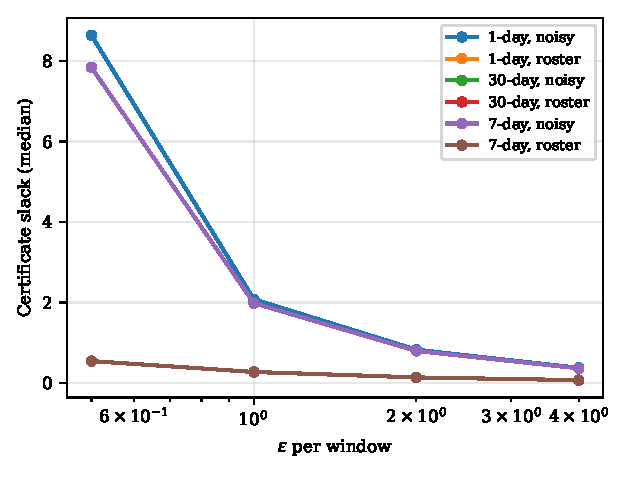
\includegraphics[width=0.95\columnwidth]{figures/cert_slack.pdf}
\caption{Median certificate slack of Proposition~\ref{prop:s-dp} as a function of the privacy budget per reporting window (r4.2, functional units), with roster denominators and with noisy active sizes, for windows of 1, 7 and 30 days. With rosters, the slack does not depend on the window length, so the three roster curves coincide.}
\label{fig:s-slack}
\end{figure}

\subsection{Evasion}
Table~\ref{tab:s-rq5thr} lists the number of insiders lost or gained when FAIR-IRS allocation replaces the global policy, for the three detectors whose evasion we analyze. Table~\ref{tab:s-rq5} reports the recall of the $45$ farming insiders, that is, the test insiders with at least three benign days before their first malicious day, for both detectors and every setting of $\alpha$, $\gamma$ and $\tau_{\mathrm{ov}}$; ``none'' disables the override ($\tau_{\mathrm{ov}}=1.01$). The column ``No farming, sched.'' gives the recall with scheduling and without farming. Against IF, scheduling raises recall with or without farming, and farming costs at most three insiders. Against GBM, the loss from farming is largest without the override, and with $\alpha=0.5$ it never exceeds two insiders. Table~\ref{tab:s-timing} reports the timing attacks of simulation S7 for six policies and three detectors; for random timing, the mean and standard deviation over five draws are given. Table~\ref{tab:s-flood} reports flooding, together with a variant of label-free FAIR-IRS in which each employee contributes at most three alerts per month to the group's cumulative count. The cap does not protect against flooding and increases the false-alert disparity, so we do not recommend it.

\begin{table}[!t]
\caption{Insiders Lost or Gained When FAIR-IRS Replaces Global Top-$k$ (r4.2)\label{tab:s-rq5thr}}
\centering
\setlength{\tabcolsep}{4pt}
\begin{tabular}{lcccc}
\toprule
Detector & Recall, global & Recall, FAIR-IRS & Lost & Gained \\
\midrule
IF & 0.176 & 0.137 & 2 & 0 \\
GBM & 0.961 & 0.980 & 1 & 2 \\
LSTM & 0.706 & 0.627 & 5 & 1 \\
\bottomrule
\end{tabular}
\end{table}
\begin{table}[!t]
\caption{Recall of Farming Insiders for All Settings (r4.2); Recall Without Farming Is 0.156 (IF) and 0.978 (GBM) Without Scheduling\label{tab:s-rq5}}
\centering
\resizebox{\columnwidth}{!}{%
\begin{tabular}{lcccccc}
\toprule
Detector & $\alpha$ & $\gamma$ & $\tau_{\mathrm{ov}}$ & No farming, sched. & Farming, no sched. & Farming, sched. \\
\midrule
GBM & 0.5 & 0.7 & 0.995 & 0.978 & 0.978 & 0.978 \\
GBM & 0.5 & 0.7 & 0.999 & 0.978 & 0.978 & 0.956 \\
GBM & 0.5 & 0.7 & none & 0.978 & 0.978 & 0.933 \\
GBM & 0.5 & 0.8 & 0.995 & 0.978 & 0.978 & 0.978 \\
GBM & 0.5 & 0.8 & 0.999 & 0.978 & 0.978 & 0.956 \\
GBM & 0.5 & 0.8 & none & 0.978 & 0.978 & 0.956 \\
GBM & 0.5 & 0.9 & 0.995 & 0.956 & 0.978 & 0.978 \\
GBM & 0.5 & 0.9 & 0.999 & 0.978 & 0.978 & 0.956 \\
GBM & 0.5 & 0.9 & none & 0.978 & 0.978 & 0.978 \\
GBM & 1 & 0.7 & 0.995 & 0.978 & 0.911 & 0.956 \\
GBM & 1 & 0.7 & 0.999 & 0.978 & 0.911 & 0.956 \\
GBM & 1 & 0.7 & none & 0.978 & 0.911 & 0.644 \\
GBM & 1 & 0.8 & 0.995 & 0.978 & 0.911 & 0.956 \\
GBM & 1 & 0.8 & 0.999 & 0.978 & 0.911 & 0.956 \\
GBM & 1 & 0.8 & none & 0.978 & 0.911 & 0.667 \\
GBM & 1 & 0.9 & 0.995 & 0.956 & 0.911 & 0.933 \\
GBM & 1 & 0.9 & 0.999 & 0.978 & 0.911 & 0.933 \\
GBM & 1 & 0.9 & none & 0.978 & 0.911 & 0.756 \\
IF & 0.5 & 0.7 & 0.995 & 0.333 & 0.156 & 0.333 \\
IF & 0.5 & 0.7 & 0.999 & 0.289 & 0.156 & 0.311 \\
IF & 0.5 & 0.7 & none & 0.267 & 0.156 & 0.267 \\
IF & 0.5 & 0.8 & 0.995 & 0.267 & 0.156 & 0.267 \\
IF & 0.5 & 0.8 & 0.999 & 0.311 & 0.156 & 0.244 \\
IF & 0.5 & 0.8 & none & 0.267 & 0.156 & 0.267 \\
IF & 0.5 & 0.9 & 0.995 & 0.244 & 0.156 & 0.244 \\
IF & 0.5 & 0.9 & 0.999 & 0.222 & 0.156 & 0.222 \\
IF & 0.5 & 0.9 & none & 0.200 & 0.156 & 0.200 \\
IF & 1 & 0.7 & 0.995 & 0.333 & 0.156 & 0.333 \\
IF & 1 & 0.7 & 0.999 & 0.289 & 0.156 & 0.267 \\
IF & 1 & 0.7 & none & 0.267 & 0.156 & 0.267 \\
IF & 1 & 0.8 & 0.995 & 0.267 & 0.156 & 0.267 \\
IF & 1 & 0.8 & 0.999 & 0.311 & 0.156 & 0.244 \\
IF & 1 & 0.8 & none & 0.267 & 0.156 & 0.244 \\
IF & 1 & 0.9 & 0.995 & 0.244 & 0.156 & 0.222 \\
IF & 1 & 0.9 & 0.999 & 0.222 & 0.156 & 0.222 \\
IF & 1 & 0.9 & none & 0.200 & 0.156 & 0.178 \\
\bottomrule
\end{tabular}}
\end{table}
\begin{table}[!t]
\caption{Insiders Detected Under Timing Attacks for All Policies (r4.2; Random: Mean $\pm$ SD Over Five Draws)\label{tab:s-timing}}
\centering
\resizebox{\columnwidth}{!}{%
\begin{tabular}{lcccccc}
\toprule
Detector & Policy & none & knows allocation & reads reports & random (mean) & $\Delta_{\mathrm{FAR}}$ \\
\midrule
GBM & B0 global & 49 & 49 & 46 & 48.4 $\pm$ 0.9 & 0.018 \\
GBM & B4 label-free, $\delta$ 0.002 & 50 & 38 & 44 & 48.6 $\pm$ 1.3 & 0.003 \\
GBM & B4 label-free, $\delta$ 0.005 & 50 & 45 & 45 & 48.6 $\pm$ 1.7 & 0.005 \\
GBM & B4 label-free, $\delta$ 0.01 & 50 & 42 & 46 & 48.0 $\pm$ 1.2 & 0.009 \\
GBM & B4 label-free, floor 2 & 51 & 35 & 43 & 48.6 $\pm$ 1.7 & 0.003 \\
GBM & B4c outcome-aware, $\delta$ 0.002 & 49 & 44 & 46 & 48.4 $\pm$ 1.1 & 0.002 \\
LSTM & B0 global & 36 & 35 & 30 & 33.8 $\pm$ 2.2 & 0.013 \\
LSTM & B4 label-free, $\delta$ 0.002 & 32 & 29 & 26 & 31.0 $\pm$ 2.0 & 0.002 \\
LSTM & B4 label-free, $\delta$ 0.005 & 34 & 31 & 27 & 32.6 $\pm$ 1.1 & 0.005 \\
LSTM & B4 label-free, $\delta$ 0.01 & 35 & 31 & 28 & 33.2 $\pm$ 1.5 & 0.009 \\
LSTM & B4 label-free, floor 2 & 32 & 31 & 29 & 29.8 $\pm$ 1.6 & 0.002 \\
LSTM & B4c outcome-aware, $\delta$ 0.002 & 34 & 28 & 27 & 32.2 $\pm$ 1.6 & 0.002 \\
IF & B0 global & 9 & 10 & 10 & 9.6 $\pm$ 0.5 & 0.045 \\
IF & B4 label-free, $\delta$ 0.002 & 7 & 7 & 7 & 6.2 $\pm$ 0.8 & 0.002 \\
IF & B4 label-free, $\delta$ 0.005 & 7 & 6 & 8 & 6.2 $\pm$ 0.8 & 0.005 \\
IF & B4 label-free, $\delta$ 0.01 & 7 & 8 & 8 & 7.0 $\pm$ 0.7 & 0.010 \\
IF & B4 label-free, floor 2 & 7 & 4 & 5 & 5.8 $\pm$ 0.8 & 0.002 \\
IF & B4c outcome-aware, $\delta$ 0.002 & 7 & 7 & 7 & 6.2 $\pm$ 0.8 & 0.002 \\
\bottomrule
\end{tabular}}
\end{table}
\begin{table}[!t]
\caption{Insiders Detected When Three Colleagues of Each Insider Flood the Group With Alerts During the Ten Preceding Days (r4.2, Mean of Five Draws)\label{tab:s-flood}}
\centering
\setlength{\tabcolsep}{4pt}
\begin{tabular}{lcccc}
\toprule
Detector & Policy & No attack & Flooding & $\Delta_{\mathrm{FAR}}$ \\
\midrule
GBM & B0 global & 49.0 & 35.6 & 0.018 \\
GBM & B4 label-free & 50.0 & 37.0 & 0.003 \\
GBM & B4 label-free, cap 3 & 50.0 & 38.2 & 0.012 \\
LSTM & B0 global & 36.0 & 22.6 & 0.013 \\
LSTM & B4 label-free & 32.0 & 23.8 & 0.002 \\
LSTM & B4 label-free, cap 3 & 33.0 & 22.4 & 0.005 \\
IF & B0 global & 9.0 & 3.0 & 0.045 \\
IF & B4 label-free & 7.0 & 6.0 & 0.002 \\
IF & B4 label-free, cap 3 & 7.0 & 5.8 & 0.008 \\
\bottomrule
\end{tabular}
\end{table}

Table~\ref{tab:s-attacks} adds an attacker who observes how often colleagues of their group were investigated in the past 30 days and acts when that rate peaks, and evaluates score floors, a larger tolerance and a tolerance drawn uniformly in $[0,2\delta]$ each day. The observing attacker gains little over the global policy; a larger tolerance limits the fully informed attacker, whereas floors and randomization do not.

\begin{table}[!t]
\caption{Insiders Detected Under Sequential Attackers, With Score Floors and Randomized Tolerance (r4.2; Random: Mean $\pm$ SD Over Five Draws)\label{tab:s-attacks}}
\centering
\resizebox{\columnwidth}{!}{%
\begin{tabular}{lccccccc}
\toprule
Detector & Policy & None & Knows allocation & Observes colleagues & Random & $\Delta_{\mathrm{FAR}}$ & Alerts used \\
\midrule
GBM & B0 global & 49 & 49 & 49 & 48.4 $\pm$ 0.9 & 0.018 & 1.000 \\
GBM & B4 label-free & 50 & 38 & 47 & 48.6 $\pm$ 1.3 & 0.003 & 1.000 \\
GBM & B4c outcome-aware & 49 & 44 & 46 & 48.4 $\pm$ 1.1 & 0.002 & 1.000 \\
GBM & B4 label-free, floor 2 & 51 & 35 & 46 & 48.6 $\pm$ 1.7 & 0.003 & 0.976 \\
GBM & B4c outcome-aware, floor 2 & 48 & 43 & 50 & 47.4 $\pm$ 1.8 & 0.002 & 0.984 \\
GBM & B4c outcome-aware, $\delta$ 0.005 & 49 & 46 & 48 & 47.6 $\pm$ 1.5 & 0.005 & 1.000 \\
GBM & B4c outcome-aware, randomized $\delta$ & 49 & 45 & 47 & 47.8 $\pm$ 2.3 & 0.002 & 1.000 \\
LSTM & B0 global & 36 & 35 & 30 & 33.8 $\pm$ 2.2 & 0.013 & 1.000 \\
LSTM & B4 label-free & 32 & 29 & 29 & 31.0 $\pm$ 2.0 & 0.002 & 1.000 \\
LSTM & B4c outcome-aware & 34 & 28 & 30 & 32.2 $\pm$ 1.6 & 0.002 & 1.000 \\
LSTM & B4 label-free, floor 2 & 32 & 31 & 27 & 29.8 $\pm$ 1.6 & 0.002 & 0.939 \\
LSTM & B4c outcome-aware, floor 2 & 32 & 32 & 29 & 29.6 $\pm$ 1.7 & 0.002 & 0.931 \\
LSTM & B4c outcome-aware, $\delta$ 0.005 & 33 & 30 & 32 & 32.2 $\pm$ 1.3 & 0.005 & 1.000 \\
LSTM & B4c outcome-aware, randomized $\delta$ & 36 & 29 & 31 & 31.6 $\pm$ 1.8 & 0.001 & 1.000 \\
\bottomrule
\end{tabular}}
\end{table}

\emph{Fairness--security frontier.} Table~\ref{tab:s-frontier} reports, for GBM and the LSTM, both modes, $\delta\in\{0.002,0.005,0.01\}$ and a protected share of $0$ to $75\%$ of the budget, the insiders detected under each timing attacker and the worst-case and mean loss with respect to no attack. Without protection, relaxing $\delta$ reduces GBM's worst-case loss from $12$ insiders to $5$ in the label-free mode and from $5$ to $3$ in the outcome-aware mode. Protection helps only when the tolerance is loose: in the outcome-aware mode with $\delta=0.01$, protecting $25$ or $50\%$ of the budget reduces GBM's worst-case loss to $2$ or $1$ insiders with $\Delta_{\FAR}=0.010$, still $45\%$ below the global policy's $0.018$. At $\delta=0.002$, protection makes parity infeasible on up to $172$ of the $251$ days, because the protected alerts concentrate on the groups that are already over-alerted, and the colleague-observing attacker then gains up to $10$ insiders. For the LSTM, the losses are between $3$ and $9$ insiders in every setting, including the global policy's $6$, so the attack exploits the detector more than the allocation. No setting combines tight parity with a small worst-case loss.

\emph{Score ties.} Proposition~2 of the main paper assumes distinct scores. No tie occurred at the alert threshold on any test day (Table~\ref{tab:s-ties}); ties would be broken by row order, and scores above every training score keep their raw order through a small order-preserving term. Alerted scores have a median between $0.991$ and $0.997$, and $8$ to $29\%$ of them exceed $\tau_{\mathrm{ov}}=0.999$, so the score mass of alerted employees is nearly flat, which weakens it as a surrogate for detections; deficit apportionment, which ignores it, performed as well (Table~\ref{tab:s-windows}).

\begin{table}[!t]
\caption{Score Ties at the Alert Threshold and Scores of Alerted User-Days Under Global Top-$k$ (r4.2, 251 Test Days)\label{tab:s-ties}}
\centering
\resizebox{\columnwidth}{!}{%
\begin{tabular}{lcccc}
\toprule
Detector & Days with tie & Alerts $\ge0.999$ & Min. alerted & Median alerted \\
\midrule
IF & 0 & 0.076 & 0.809 & 0.991 \\
AE & 0 & 0.090 & 0.874 & 0.994 \\
LR & 0 & 0.137 & 0.255 & 0.995 \\
GBM & 0 & 0.293 & 0.621 & 0.997 \\
LSTM & 0 & 0.125 & 0.958 & 0.992 \\
\bottomrule
\end{tabular}}
\end{table}

\emph{Attackers over several draws, paired with the global policy.} Relocating an episode changes detection even under the global policy, because the insider's scores compete with different colleagues on different days: in our draws, the global policy lost up to eight insiders on relocated episodes. Table~\ref{tab:s-attacks2} therefore scores every relocated attack under the parity rule P and under the global policy B0, and reports the excess loss $\sum_i[(h^{P}_{i}-h^{B0}_{i})-(\tilde h^{P}_{i}-\tilde h^{B0}_{i})]$, where $h$ and $\tilde h$ indicate the detection of insider $i$ without and with the attack, with a paired bootstrap interval over insiders. Each attacker chooses the start of its episode from P's unattacked run; ties are broken at random, and each attacker is drawn five times (the random attacker ten times). The \emph{deficit-estimating} attacker reads monthly reports of P's alert counts, released with Laplace noise at $\varepsilon=1$, adds the investigations of colleagues observed since the last report, and acts where its group's estimated accumulated rate exceeds the overall rate the most. The only excess loss whose interval excludes zero is that of the allocation-aware attacker against the label-free mode for GBM ($+9.6$, interval $3.6$ to $15.8$). Against the outcome-aware mode, the same attacker's excess is $+1.2$ for GBM and $+1.8$ for the LSTM. The deficit-estimating attacker, who needs only reports and observations, gains $+4.0$ ($-0.6$ to $8.6$) against label-free GBM and at most $+1.2$ against the outcome-aware mode.

\emph{Randomized displacement.} A cut group may keep $k_g$ alerts drawn uniformly at random among its $K_g$ members in the global top-$k$, instead of its $k_g$ highest scores; the counts $k_g$, and hence parity, are unchanged.

\begin{proposition}[Randomized displacement]
\label{prop:s-random}
Consider a parity rule in the label-free mode, without suppression, and scores that do not depend on the draws (in particular, the insider's timing is fixed in advance or chosen from information independent of the draws). Let insider $i$ of group $g$ be in the global top-$k$ in the windows of a set $\mathcal{H}$, and let $c_{g,t}=1-k_{g,t}/K_{g,t}$ be the cut fraction of $g$ in window $t$ ($c_{g,t}=0$ if $k_{g,t}\ge K_{g,t}$). Under randomized displacement, the probability that $i$ is alerted in no window of $\mathcal{H}$ is $\mathbb{E}\big[\prod_{t\in\mathcal{H}}c_{g,t}\big]$, the expectation being over the scores.
\end{proposition}
\begin{IEEEproof}
In the label-free mode, $A_{g,t}$ counts all alerts sent to $g$, which equal $\sum_{t'<t}k_{g,t'}$ whichever members were drawn, and $D_{g,t}$ does not depend on alerts. Given the scores, the counts $K_{g,t}$ and $k_{g,t}$ of every window are therefore the same on every realization of the draws, and so is each $c_{g,t}$. In window $t\in\mathcal{H}$, $i$ is one of the $K_{g,t}$ candidates of $g$; if $k_{g,t}\ge K_{g,t}$, every candidate is alerted, and otherwise $k_{g,t}$ of them are drawn uniformly with fresh randomness, so $i$ is passed over with probability $c_{g,t}$, independently of the other windows. The probability of being passed over in every window of $\mathcal{H}$ is the product of the $c_{g,t}$ given the scores, and taking the expectation over the scores gives the claim. In the outcome-aware mode, a confirmed alert on $i$ removes it from $A_g$ and $D_g$, and under a cooldown a cleared alert suppresses its recipient later; in both cases the later counts depend on the earlier draws, the factorization fails, and the product is not a bound.
\end{IEEEproof}

The probability is small only if the cut fractions stay below one, and in every randomized run some group lost all its alerts on some day ($c_{g,t}=1$). Summed over the insiders caught by the global policy, the realized products were close to the observed misses (for example, $9.3$ against $8.6$ for the allocation-aware attacker on label-free GBM), and randomization cost GBM three insiders without attack (Table~\ref{tab:s-attacks2}).

\begin{table}[!t]
\caption{Timing Attackers Over Several Draws (r4.2, Functional Units, $\delta$ = 0.002). Insiders Detected Under Policy P and Under the Global Policy (B0), Without and With the Attack, on the Same Relocated Episodes; Excess Loss: Insiders Lost Under P Beyond Those Lost Under B0, Mean Over Draws With a Paired Bootstrap Interval Over Insiders and the Range Over Draws; Bound / Obs.: Expected Misses Under the Bound of Proposition~S1 and Observed Misses Among Insiders Caught by B0\label{tab:s-attacks2}}
\centering
\resizebox{\columnwidth}{!}{%
\begin{tabular}{lcccccccccc}
\toprule
Detector & Policy & Attacker & Draws & P & B0 & P att. & B0 att. & Excess loss [95\% CI] & Range & Bound / obs. \\
\midrule
GBM & B4 LF & knows allocation & 5 & 50 & 49 & 37.6 & 46.2 & +9.6 [+3.6, +15.8] & +8 to +10 & -- \\
GBM & B4 LF & observes colleagues & 5 & 50 & 49 & 47 & 49 & +3.0 [-2.0, +8.0] & +3 to +3 & -- \\
GBM & B4 LF & reads reports & 5 & 50 & 49 & 47.6 & 48 & +1.4 [-2.2, +5.0] & -1 to +3 & -- \\
GBM & B4 LF & estimates deficit & 5 & 50 & 49 & 44 & 47 & +4.0 [-0.6, +8.6] & +2 to +6 & -- \\
GBM & B4 LF & random & 10 & 50 & 49 & 48.4 & 48.5 & +1.1 [-2.2, +4.7] & -1 to +3 & -- \\
GBM & B4c OA & knows allocation & 5 & 49 & 49 & 44.2 & 45.4 & +1.2 [-3.2, +5.6] & -1 to +3 & -- \\
GBM & B4c OA & observes colleagues & 5 & 49 & 49 & 46 & 47.8 & +1.8 [-3.2, +6.8] & +1 to +2 & -- \\
GBM & B4c OA & reads reports & 5 & 49 & 49 & 47.6 & 48.4 & +0.8 [-2.8, +4.6] & -1 to +4 & -- \\
GBM & B4c OA & estimates deficit & 5 & 49 & 49 & 44 & 45 & +1.0 [-2.6, +4.4] & -1 to +3 & -- \\
GBM & B4c OA & random & 10 & 49 & 49 & 48.5 & 48.5 & +0.0 [-3.8, +3.8] & -2 to +2 & -- \\
GBM & B4 LF, random displ. & knows allocation & 5 & 47 & 49 & 39 & 46.2 & +5.2 [-0.6, +11.2] & +3 to +7 & 9.3 / 8.6 \\
GBM & B4 LF, random displ. & observes colleagues & 5 & 47 & 49 & 44.6 & 49 & +2.4 [-3.8, +8.4] & +1 to +3 & 5.8 / 5.4 \\
GBM & B4 LF, random displ. & reads reports & 5 & 47 & 49 & 46.2 & 48 & -0.2 [-5.2, +4.8] & -1 to +1 & 2.7 / 2.4 \\
GBM & B4 LF, random displ. & estimates deficit & 5 & 47 & 49 & 41.6 & 47 & +3.4 [-2.0, +8.8] & +0 to +6 & 5.7 / 6.0 \\
GBM & B4 LF, random displ. & random & 10 & 47 & 49 & 46.3 & 48.5 & +0.2 [-4.5, +5.1] & -2 to +4 & 2.9 / 3.3 \\
GBM & B4c OA, random displ. & knows allocation & 5 & 46 & 49 & 43.2 & 47.8 & +1.6 [-4.4, +7.8] & +1 to +2 & 4.8 / 5.6 \\
GBM & B4c OA, random displ. & observes colleagues & 5 & 46 & 49 & 42.2 & 47 & +1.8 [-4.0, +7.6] & +1 to +3 & 6.5 / 5.8 \\
GBM & B4c OA, random displ. & reads reports & 5 & 46 & 49 & 44.6 & 48.4 & +0.8 [-5.2, +6.6] & -1 to +2 & 4.4 / 4.6 \\
GBM & B4c OA, random displ. & estimates deficit & 5 & 46 & 49 & 44.8 & 47.6 & -0.2 [-5.8, +5.4] & -2 to +2 & 4.4 / 3.8 \\
GBM & B4c OA, random displ. & random & 10 & 46 & 49 & 46.4 & 48.5 & -0.9 [-6.4, +4.6] & -2 to +1 & 2.8 / 2.7 \\
LSTM & B4 LF & knows allocation & 5 & 32 & 36 & 30.4 & 34.8 & +0.4 [-4.4, +5.2] & -2 to +2 & -- \\
LSTM & B4 LF & observes colleagues & 5 & 32 & 36 & 29 & 33.2 & +0.2 [-3.6, +4.0] & +0 to +1 & -- \\
LSTM & B4 LF & reads reports & 5 & 32 & 36 & 31.8 & 33.2 & -2.6 [-6.4, +0.8] & -5 to -1 & -- \\
LSTM & B4 LF & estimates deficit & 5 & 32 & 36 & 28.4 & 32 & -0.4 [-5.4, +4.8] & -2 to +1 & -- \\
LSTM & B4 LF & random & 10 & 32 & 36 & 31.9 & 34 & -1.9 [-6.6, +2.4] & -4 to +0 & -- \\
LSTM & B4c OA & knows allocation & 5 & 34 & 36 & 29.2 & 33 & +1.8 [-2.2, +6.0] & +0 to +3 & -- \\
LSTM & B4c OA & observes colleagues & 5 & 34 & 36 & 30 & 34.4 & +2.4 [-3.6, +8.4] & +2 to +3 & -- \\
LSTM & B4c OA & reads reports & 5 & 34 & 36 & 32 & 34 & +0.0 [-3.8, +3.8] & -2 to +3 & -- \\
LSTM & B4c OA & estimates deficit & 5 & 34 & 36 & 31.2 & 34.4 & +1.2 [-2.6, +5.4] & -1 to +4 & -- \\
LSTM & B4c OA & random & 10 & 34 & 36 & 33.1 & 34 & -1.1 [-5.4, +3.1] & -4 to +1 & -- \\
LSTM & B4 LF, random displ. & knows allocation & 5 & 33 & 36 & 29.4 & 34.8 & +2.4 [-3.4, +8.4] & +0 to +6 & 8.0 / 8.0 \\
LSTM & B4 LF, random displ. & observes colleagues & 5 & 33 & 36 & 29 & 33.2 & +1.2 [-3.8, +6.0] & +0 to +2 & 6.6 / 6.2 \\
LSTM & B4 LF, random displ. & reads reports & 5 & 33 & 36 & 30.8 & 33.2 & -0.6 [-5.6, +4.4] & -1 to +1 & 4.8 / 4.6 \\
LSTM & B4 LF, random displ. & estimates deficit & 5 & 33 & 36 & 27.8 & 32 & +1.2 [-4.0, +6.6] & +0 to +3 & 6.1 / 6.0 \\
LSTM & B4 LF, random displ. & random & 10 & 33 & 36 & 30.7 & 34 & +0.3 [-4.5, +5.1] & -2 to +4 & 4.2 / 4.5 \\
LSTM & B4c OA, random displ. & knows allocation & 5 & 35 & 36 & 30.6 & 34.2 & +2.6 [-1.8, +7.4] & +1 to +5 & 6.2 / 5.8 \\
LSTM & B4c OA, random displ. & observes colleagues & 5 & 35 & 36 & 26.2 & 28 & +0.8 [-4.2, +5.8] & -1 to +3 & 3.4 / 3.8 \\
LSTM & B4c OA, random displ. & reads reports & 5 & 35 & 36 & 33.2 & 34.6 & +0.4 [-3.6, +4.2] & -1 to +2 & 3.8 / 3.0 \\
LSTM & B4c OA, random displ. & estimates deficit & 5 & 35 & 36 & 31.2 & 33.4 & +1.2 [-3.6, +6.0] & -2 to +4 & 4.2 / 4.4 \\
LSTM & B4c OA, random displ. & random & 10 & 35 & 36 & 32 & 34 & +1.0 [-3.6, +5.7] & -4 to +5 & 4.2 / 4.2 \\
\bottomrule
\end{tabular}}
\end{table}


\begin{table}[!t]
\caption{Fairness--Security Frontier: Insiders Detected Under Each Attacker and Worst-Case and Mean Loss, by Mode, Tolerance and Share of the Budget Protected for the Global Top Scores (r4.2)\label{tab:s-frontier}}
\centering
\resizebox{\columnwidth}{!}{%
\begin{tabular}{lccccccccccc}
\toprule
Detector & Mode & $\delta$ & Protected & $\Delta_{\mathrm{FAR}}$ & Fallback days & No attack & Knows alloc. & Observes & Random & Worst loss & Mean loss \\
\midrule
GBM & global & -- & 0\% & 0.0180 & 0 & 49 & 49 & 49 & 48.7 & 0.3 & 0.1 \\
GBM & label-free & 0.002 & 0\% & 0.0029 & 7 & 50 & 38 & 47 & 48.3 & 12.0 & 5.6 \\
GBM & label-free & 0.002 & 25\% & 0.0027 & 46 & 51 & 38 & 42 & 48.3 & 13.0 & 8.2 \\
GBM & label-free & 0.002 & 50\% & 0.0045 & 172 & 50 & 48 & 40 & 48.0 & 10.0 & 4.7 \\
GBM & label-free & 0.002 & 75\% & 0.0114 & 172 & 51 & 49 & 47 & 48.7 & 4.0 & 2.8 \\
GBM & label-free & 0.005 & 0\% & 0.0055 & 2 & 50 & 45 & 47 & 48.0 & 5.0 & 3.3 \\
GBM & label-free & 0.005 & 25\% & 0.0055 & 29 & 51 & 35 & 41 & 48.3 & 16.0 & 9.6 \\
GBM & label-free & 0.005 & 50\% & 0.0045 & 168 & 50 & 48 & 40 & 48.0 & 10.0 & 4.7 \\
GBM & label-free & 0.005 & 75\% & 0.0114 & 172 & 51 & 49 & 47 & 48.7 & 4.0 & 2.8 \\
GBM & label-free & 0.01 & 0\% & 0.0093 & 1 & 50 & 42 & 49 & 47.7 & 8.0 & 3.8 \\
GBM & label-free & 0.01 & 25\% & 0.0086 & 14 & 50 & 40 & 46 & 48.3 & 10.0 & 5.2 \\
GBM & label-free & 0.01 & 50\% & 0.0073 & 91 & 50 & 40 & 44 & 48.3 & 10.0 & 5.9 \\
GBM & label-free & 0.01 & 75\% & 0.0114 & 172 & 51 & 49 & 47 & 49.0 & 4.0 & 2.7 \\
GBM & outcome-aware & 0.002 & 0\% & 0.0020 & 8 & 49 & 44 & 46 & 48.0 & 5.0 & 3.0 \\
GBM & outcome-aware & 0.002 & 25\% & 0.0020 & 8 & 50 & 47 & 44 & 47.3 & 6.0 & 3.9 \\
GBM & outcome-aware & 0.002 & 50\% & 0.0042 & 154 & 50 & 47 & 40 & 48.0 & 10.0 & 5.0 \\
GBM & outcome-aware & 0.002 & 75\% & 0.0118 & 172 & 49 & 48 & 44 & 48.3 & 5.0 & 2.2 \\
GBM & outcome-aware & 0.005 & 0\% & 0.0050 & 4 & 49 & 46 & 48 & 47.7 & 3.0 & 1.8 \\
GBM & outcome-aware & 0.005 & 25\% & 0.0050 & 5 & 49 & 46 & 45 & 47.3 & 4.0 & 2.9 \\
GBM & outcome-aware & 0.005 & 50\% & 0.0055 & 99 & 50 & 48 & 43 & 48.3 & 7.0 & 3.6 \\
GBM & outcome-aware & 0.005 & 75\% & 0.0118 & 168 & 51 & 47 & 45 & 49.0 & 6.0 & 4.0 \\
GBM & outcome-aware & 0.01 & 0\% & 0.0100 & 1 & 49 & 44 & 47 & 47.7 & 5.0 & 2.8 \\
GBM & outcome-aware & 0.01 & 25\% & 0.0098 & 1 & 49 & 47 & 49 & 48.0 & 2.0 & 1.0 \\
GBM & outcome-aware & 0.01 & 50\% & 0.0100 & 25 & 49 & 48 & 49 & 48.0 & 1.0 & 0.7 \\
GBM & outcome-aware & 0.01 & 75\% & 0.0120 & 142 & 50 & 48 & 50 & 48.7 & 2.0 & 1.1 \\
LSTM & global & -- & 0\% & 0.0129 & 0 & 36 & 35 & 30 & 34.0 & 6.0 & 3.0 \\
LSTM & label-free & 0.002 & 0\% & 0.0022 & 7 & 32 & 29 & 29 & 31.7 & 3.0 & 2.1 \\
LSTM & label-free & 0.002 & 25\% & 0.0019 & 9 & 35 & 32 & 29 & 30.7 & 6.0 & 4.4 \\
LSTM & label-free & 0.002 & 50\% & 0.0018 & 78 & 36 & 30 & 27 & 32.7 & 9.0 & 6.1 \\
LSTM & label-free & 0.002 & 75\% & 0.0064 & 172 & 34 & 31 & 28 & 33.3 & 6.0 & 3.2 \\
LSTM & label-free & 0.005 & 0\% & 0.0049 & 2 & 34 & 31 & 31 & 32.7 & 3.0 & 2.4 \\
LSTM & label-free & 0.005 & 25\% & 0.0045 & 6 & 35 & 30 & 31 & 32.3 & 5.0 & 3.9 \\
LSTM & label-free & 0.005 & 50\% & 0.0044 & 25 & 36 & 30 & 27 & 33.0 & 9.0 & 6.0 \\
LSTM & label-free & 0.005 & 75\% & 0.0064 & 172 & 34 & 31 & 28 & 33.3 & 6.0 & 3.2 \\
LSTM & label-free & 0.01 & 0\% & 0.0094 & 1 & 35 & 31 & 32 & 33.3 & 4.0 & 2.9 \\
LSTM & label-free & 0.01 & 25\% & 0.0095 & 1 & 34 & 30 & 31 & 32.3 & 4.0 & 2.9 \\
LSTM & label-free & 0.01 & 50\% & 0.0094 & 2 & 37 & 30 & 31 & 33.0 & 7.0 & 5.7 \\
LSTM & label-free & 0.01 & 75\% & 0.0094 & 43 & 35 & 30 & 28 & 33.3 & 7.0 & 4.6 \\
LSTM & outcome-aware & 0.002 & 0\% & 0.0020 & 6 & 34 & 28 & 30 & 32.0 & 6.0 & 4.0 \\
LSTM & outcome-aware & 0.002 & 25\% & 0.0020 & 7 & 35 & 29 & 32 & 32.7 & 6.0 & 3.8 \\
LSTM & outcome-aware & 0.002 & 50\% & 0.0020 & 50 & 34 & 33 & 31 & 32.3 & 3.0 & 1.9 \\
LSTM & outcome-aware & 0.002 & 75\% & 0.0064 & 172 & 34 & 31 & 27 & 33.7 & 7.0 & 3.4 \\
LSTM & outcome-aware & 0.005 & 0\% & 0.0050 & 4 & 33 & 30 & 32 & 32.0 & 3.0 & 1.7 \\
LSTM & outcome-aware & 0.005 & 25\% & 0.0050 & 4 & 35 & 32 & 31 & 31.7 & 4.0 & 3.4 \\
LSTM & outcome-aware & 0.005 & 50\% & 0.0050 & 16 & 37 & 30 & 29 & 33.3 & 8.0 & 6.2 \\
LSTM & outcome-aware & 0.005 & 75\% & 0.0064 & 172 & 34 & 31 & 27 & 33.3 & 7.0 & 3.6 \\
LSTM & outcome-aware & 0.01 & 0\% & 0.0100 & 1 & 35 & 30 & 28 & 32.7 & 7.0 & 4.8 \\
LSTM & outcome-aware & 0.01 & 25\% & 0.0100 & 2 & 34 & 30 & 29 & 33.0 & 5.0 & 3.3 \\
LSTM & outcome-aware & 0.01 & 50\% & 0.0100 & 3 & 36 & 27 & 31 & 33.0 & 9.0 & 5.7 \\
LSTM & outcome-aware & 0.01 & 75\% & 0.0100 & 35 & 35 & 33 & 29 & 33.3 & 6.0 & 3.2 \\
\bottomrule
\end{tabular}}
\end{table}

\subsection{Variability, Budget, Training Regime and Intersectional Groups}
Table~\ref{tab:s-seeds} reports the mean and 95\% confidence interval over five seeds for the detectors whose training is random; LR is deterministic and is reported once. Under FAIR-IRS, the disparity has almost no variance across seeds, whereas under the global policy it varies widely (GBM: $\rho_{\FAR}=5.5\pm2.0$). Table~\ref{tab:s-budget} reports the effect of the budget, with $\delta=0.2\,b$. FAIR-IRS keeps $\Delta_{\AR}$ at $0.2\,b$ for every budget and detector; its largest detection cost is four insiders, for GBM at $b=0.5\%$, and it costs nothing at $b=2\%$ for GBM, AE and the LSTM. Table~\ref{tab:s-contam} compares the unsupervised detectors trained on benign training days with the same detectors trained on all training days, without labels. Table~\ref{tab:s-inter} reports the burden across the cells of functional unit $\times$ after-hours work, with FAIR-IRS enforcing parity either on functional units only or on the cells. The LSTM, absent from Table~\ref{tab:s-seeds}, was retrained with four more seeds for the non-inferiority analysis (Table~\ref{tab:s-noninf}).

Table~\ref{tab:s-valid} chooses the tolerance on the first half of the test period ($39$ insiders) and evaluates it on the second ($17$ insiders). The rule, the smallest $\delta$ whose one-sided lower bound on the validation recall difference exceeds $-0.05$, selects $\delta=0.001$ for LR, $0.005$ for GBM and, because no tolerance passes for IF, AE and the LSTM, the largest value ($0.01$) for them. With so few insiders, detection cannot guide the choice of $\delta$, which we fixed at $0.2\,b$ in the protocol before any experiment.

Table~\ref{tab:s-warm} evaluates two ways of avoiding the fallback days at the start of a deployment. A shadow month, global top-$k$ for $30$ days with histories accumulated, leaves the disparity of that month in the histories, and the parity rules then fall back on up to $138$ days to repair it. Starting each history with $30$ pseudo-days at the budget rate removes fallback altogether but dilutes the histories, so that the true accumulated disparity stays near $0.0045$, about $2\delta$, on nearly every day. The default, $6$ to $8$ fallback days in the first month, is the smaller cost.

\begin{table}[!t]
\caption{Tolerance Chosen on a Validation Period (First Half of the r4.2 Test Period, 39 Insiders) and Evaluated on the Second Half (17 Insiders). $\ast$: Smallest $\delta$ Whose One-Sided 95\% Lower Bound on the Validation Recall Difference Exceeds $-0.05$ (the Largest $\delta$ if None Does)\label{tab:s-valid}}
\centering
\resizebox{\columnwidth}{!}{%
\begin{tabular}{lcccccccccc}
\toprule
Detector & Mode & $\delta$ & Chosen & Val. lost & Val. gained & Val. lower bd. & Test det. & Test det. B0 & Test $\Delta_{\mathrm{FAR}}$ & Test $\Delta_{\mathrm{FAR}}$ B0 \\
\midrule
IF & label-free & 0.001 &  & 2 & 0 & -0.1026 & 1 & 2 & 0.0011 & 0.0444 \\
IF & label-free & 0.002 &  & 1 & 0 & -0.0769 & 1 & 2 & 0.0027 & 0.0444 \\
IF & label-free & 0.005 &  & 1 & 0 & -0.0769 & 1 & 2 & 0.0051 & 0.0444 \\
IF & label-free & 0.01 & $\ast$ & 1 & 0 & -0.0769 & 1 & 2 & 0.0102 & 0.0444 \\
IF & outcome-aware & 0.001 &  & 2 & 0 & -0.1026 & 1 & 2 & 0.0010 & 0.0444 \\
IF & outcome-aware & 0.002 &  & 1 & 0 & -0.0769 & 1 & 2 & 0.0020 & 0.0444 \\
IF & outcome-aware & 0.005 &  & 1 & 0 & -0.0769 & 1 & 2 & 0.0051 & 0.0444 \\
IF & outcome-aware & 0.01 & $\ast$ & 1 & 0 & -0.0769 & 1 & 2 & 0.0101 & 0.0444 \\
AE & label-free & 0.001 &  & 2 & 4 & -0.0513 & 9 & 9 & 0.0010 & 0.0151 \\
AE & label-free & 0.002 &  & 3 & 3 & -0.1026 & 9 & 9 & 0.0020 & 0.0151 \\
AE & label-free & 0.005 &  & 3 & 1 & -0.1282 & 9 & 9 & 0.0047 & 0.0151 \\
AE & label-free & 0.01 & $\ast$ & 2 & 0 & -0.1026 & 9 & 9 & 0.0099 & 0.0151 \\
AE & outcome-aware & 0.001 &  & 2 & 1 & -0.1026 & 9 & 9 & 0.0016 & 0.0151 \\
AE & outcome-aware & 0.002 &  & 1 & 1 & -0.0513 & 9 & 9 & 0.0027 & 0.0151 \\
AE & outcome-aware & 0.005 &  & 2 & 1 & -0.1026 & 9 & 9 & 0.0050 & 0.0151 \\
AE & outcome-aware & 0.01 & $\ast$ & 1 & 0 & -0.0769 & 9 & 9 & 0.0107 & 0.0151 \\
LR & label-free & 0.001 & $\ast$ & 0 & 1 & 0.0000 & 14 & 14 & 0.0016 & 0.0091 \\
LR & label-free & 0.002 &  & 1 & 1 & -0.0513 & 14 & 14 & 0.0024 & 0.0091 \\
LR & label-free & 0.005 &  & 0 & 1 & 0.0000 & 14 & 14 & 0.0052 & 0.0091 \\
LR & label-free & 0.01 &  & 0 & 0 & 0.0000 & 14 & 14 & 0.0091 & 0.0091 \\
LR & outcome-aware & 0.001 & $\ast$ & 0 & 1 & 0.0000 & 14 & 14 & 0.0019 & 0.0091 \\
LR & outcome-aware & 0.002 &  & 0 & 1 & 0.0000 & 14 & 14 & 0.0030 & 0.0091 \\
LR & outcome-aware & 0.005 &  & 0 & 1 & 0.0000 & 14 & 14 & 0.0074 & 0.0091 \\
LR & outcome-aware & 0.01 &  & 0 & 0 & 0.0000 & 14 & 14 & 0.0091 & 0.0091 \\
GBM & label-free & 0.001 &  & 1 & 2 & -0.0513 & 16 & 16 & 0.0041 & 0.0168 \\
GBM & label-free & 0.002 &  & 1 & 2 & -0.0513 & 16 & 16 & 0.0037 & 0.0168 \\
GBM & label-free & 0.005 & $\ast$ & 0 & 1 & 0.0000 & 16 & 16 & 0.0065 & 0.0168 \\
GBM & label-free & 0.01 &  & 0 & 1 & 0.0000 & 16 & 16 & 0.0115 & 0.0168 \\
GBM & outcome-aware & 0.001 &  & 1 & 1 & -0.0513 & 15 & 16 & 0.0011 & 0.0168 \\
GBM & outcome-aware & 0.002 &  & 1 & 1 & -0.0513 & 16 & 16 & 0.0021 & 0.0168 \\
GBM & outcome-aware & 0.005 & $\ast$ & 0 & 1 & 0.0000 & 15 & 16 & 0.0052 & 0.0168 \\
GBM & outcome-aware & 0.01 &  & 0 & 0 & 0.0000 & 16 & 16 & 0.0113 & 0.0168 \\
LSTM & label-free & 0.001 &  & 3 & 1 & -0.1282 & 10 & 11 & 0.0014 & 0.0125 \\
LSTM & label-free & 0.002 &  & 5 & 1 & -0.2051 & 11 & 11 & 0.0023 & 0.0125 \\
LSTM & label-free & 0.005 &  & 3 & 1 & -0.1282 & 11 & 11 & 0.0049 & 0.0125 \\
LSTM & label-free & 0.01 & $\ast$ & 2 & 1 & -0.1026 & 11 & 11 & 0.0098 & 0.0125 \\
LSTM & outcome-aware & 0.001 &  & 4 & 2 & -0.1538 & 11 & 11 & 0.0011 & 0.0125 \\
LSTM & outcome-aware & 0.002 &  & 4 & 2 & -0.1538 & 11 & 11 & 0.0021 & 0.0125 \\
LSTM & outcome-aware & 0.005 &  & 4 & 1 & -0.1795 & 11 & 11 & 0.0052 & 0.0125 \\
LSTM & outcome-aware & 0.01 & $\ast$ & 2 & 1 & -0.1026 & 11 & 11 & 0.0104 & 0.0125 \\
\bottomrule
\end{tabular}}
\end{table}
\begin{table}[!t]
\caption{Shadow Month (Global Top-$k$ for 30 Days, Then Parity) and Prior Warm Start (Histories Begin With 30 Pseudo-Days per Group at the Budget Rate) (r4.2, $\delta$ = 0.002). Max: Largest Disparity of the Constrained Cumulative Rate, Measured on Actual Alerts\label{tab:s-warm}}
\centering
\resizebox{\columnwidth}{!}{%
\begin{tabular}{lcccccccc}
\toprule
Detector & Mode & Start & Det. & $\Delta_{\mathrm{FAR}}$ & Fallback days & Max, days 1--30 & Max, later & Days $>\delta$, later \\
\midrule
IF & label-free & none & 7 & 0.0020 & 7 & 0.0111 & 0.0020 & 0.0000 \\
IF & label-free & shadow month & 6 & 0.0019 & 138 & 0.0667 & 0.0582 & 0.6244 \\
IF & label-free & prior & 8 & 0.0024 & 0 & 0.0556 & 0.0046 & 1.0000 \\
IF & outcome-aware & none & 7 & 0.0020 & 6 & 0.0111 & 0.0020 & 0.0045 \\
IF & outcome-aware & shadow month & 7 & 0.0020 & 135 & 0.0623 & 0.0567 & 0.6154 \\
IF & outcome-aware & prior & 8 & 0.0023 & 0 & 0.0449 & 0.0047 & 1.0000 \\
AE & label-free & none & 33 & 0.0021 & 7 & 0.0111 & 0.0020 & 0.0000 \\
AE & label-free & shadow month & 31 & 0.0022 & 27 & 0.0588 & 0.0163 & 0.1222 \\
AE & label-free & prior & 34 & 0.0024 & 0 & 0.0588 & 0.0044 & 1.0000 \\
AE & outcome-aware & none & 33 & 0.0020 & 6 & 0.0111 & 0.0023 & 0.0090 \\
AE & outcome-aware & shadow month & 32 & 0.0019 & 26 & 0.0588 & 0.0144 & 0.1176 \\
AE & outcome-aware & prior & 34 & 0.0023 & 0 & 0.0588 & 0.0042 & 1.0000 \\
LR & label-free & none & 42 & 0.0020 & 7 & 0.0111 & 0.0020 & 0.0000 \\
LR & label-free & shadow month & 43 & 0.0017 & 6 & 0.0260 & 0.0083 & 0.0271 \\
LR & label-free & prior & 43 & 0.0020 & 0 & 0.0260 & 0.0043 & 0.9955 \\
LR & outcome-aware & none & 43 & 0.0019 & 8 & 0.0111 & 0.0024 & 0.0090 \\
LR & outcome-aware & shadow month & 42 & 0.0019 & 4 & 0.0260 & 0.0077 & 0.0226 \\
LR & outcome-aware & prior & 43 & 0.0023 & 0 & 0.0260 & 0.0043 & 0.9729 \\
GBM & label-free & none & 50 & 0.0029 & 7 & 0.0111 & 0.0020 & 0.0000 \\
GBM & label-free & shadow month & 49 & 0.0039 & 121 & 0.0553 & 0.0507 & 0.5475 \\
GBM & label-free & prior & 51 & 0.0030 & 0 & 0.0294 & 0.0046 & 0.9955 \\
GBM & outcome-aware & none & 49 & 0.0020 & 8 & 0.0102 & 0.0021 & 0.1448 \\
GBM & outcome-aware & shadow month & 47 & 0.0020 & 32 & 0.0155 & 0.0145 & 0.3032 \\
GBM & outcome-aware & prior & 48 & 0.0024 & 0 & 0.0095 & 0.0044 & 0.9955 \\
LSTM & label-free & none & 32 & 0.0022 & 7 & 0.0111 & 0.0020 & 0.0000 \\
LSTM & label-free & shadow month & 35 & 0.0022 & 33 & 0.0389 & 0.0188 & 0.1493 \\
LSTM & label-free & prior & 32 & 0.0025 & 0 & 0.0333 & 0.0045 & 1.0000 \\
LSTM & outcome-aware & none & 34 & 0.0020 & 6 & 0.0111 & 0.0020 & 0.0090 \\
LSTM & outcome-aware & shadow month & 32 & 0.0020 & 32 & 0.0335 & 0.0172 & 0.1584 \\
LSTM & outcome-aware & prior & 32 & 0.0024 & 0 & 0.0279 & 0.0047 & 1.0000 \\
\bottomrule
\end{tabular}}
\end{table}

\begin{table}[!t]
\caption{Mean and 95\% CI Over Five Seeds (r4.2, $\delta$ = 0.002)\label{tab:s-seeds}}
\centering
\resizebox{\columnwidth}{!}{%
\begin{tabular}{lccccccc}
\toprule
Detector & Policy & Runs & Recall & Prec. & $\Delta_{\mathrm{FAR}}$ & $\rho_{\mathrm{FAR}}$ & Gini($F$) \\
\midrule
IF & global & 5 & 0.176 $\pm$ 0.024 & 0.008 $\pm$ 0.001 & 0.044 $\pm$ 0.002 & 30.460 $\pm$ 6.784 & 0.980 $\pm$ 0.001 \\
IF & FAIR-IRS & 5 & 0.106 $\pm$ 0.037 & 0.004 $\pm$ 0.001 & 0.002 $\pm$ 0.000 & 1.217 $\pm$ 0.003 & 0.973 $\pm$ 0.001 \\
AE & global & 5 & 0.565 $\pm$ 0.153 & 0.030 $\pm$ 0.009 & 0.015 $\pm$ 0.002 & 3.736 $\pm$ 0.589 & 0.936 $\pm$ 0.005 \\
AE & FAIR-IRS & 5 & 0.573 $\pm$ 0.108 & 0.029 $\pm$ 0.008 & 0.002 $\pm$ 0.000 & 1.233 $\pm$ 0.028 & 0.933 $\pm$ 0.005 \\
GBM & global & 5 & 0.922 $\pm$ 0.096 & 0.241 $\pm$ 0.036 & 0.016 $\pm$ 0.004 & 5.510 $\pm$ 1.953 & 0.944 $\pm$ 0.007 \\
GBM & FAIR-IRS & 5 & 0.894 $\pm$ 0.112 & 0.222 $\pm$ 0.034 & 0.003 $\pm$ 0.000 & 1.381 $\pm$ 0.035 & 0.937 $\pm$ 0.006 \\
LR & global & 1 & 0.824 & 0.083 & 0.009 & 3.433 & 0.971 \\
LR & FAIR-IRS & 1 & 0.824 & 0.083 & 0.002 & 1.252 & 0.967 \\
\bottomrule
\end{tabular}}
\end{table}
\begin{table}[!t]
\caption{Effect of the Analyst Budget (r4.2, $\delta$ = 0.2 $\times$ Budget)\label{tab:s-budget}}
\centering
\resizebox{\columnwidth}{!}{%
\begin{tabular}{lccccccc}
\toprule
Detector & Budget & Policy & Recall [95\% CI] & Prec. & $\Delta_{\mathrm{FAR}}$ & $\rho_{\mathrm{FAR}}$ & $\max F_i$ \\
\midrule
IF & 0.005 & global & 0.137 [0.07, 0.26] & 0.012 & 0.034 & 65.050 & 144 \\
IF & 0.005 & FAIR-IRS & 0.098 [0.04, 0.21] & 0.007 & 0.001 & 1.214 & 134 \\
IF & 0.01 & global & 0.176 [0.10, 0.30] & 0.008 & 0.045 & 29.201 & 191 \\
IF & 0.01 & FAIR-IRS & 0.137 [0.07, 0.26] & 0.005 & 0.002 & 1.218 & 175 \\
IF & 0.02 & global & 0.216 [0.12, 0.35] & 0.005 & 0.049 & 6.363 & 211 \\
IF & 0.02 & FAIR-IRS & 0.216 [0.12, 0.35] & 0.004 & 0.004 & 1.220 & 200 \\
AE & 0.005 & global & 0.529 [0.40, 0.66] & 0.061 & 0.007 & 3.333 & 36 \\
AE & 0.005 & FAIR-IRS & 0.490 [0.36, 0.62] & 0.052 & 0.001 & 1.259 & 36 \\
AE & 0.01 & global & 0.647 [0.51, 0.76] & 0.037 & 0.014 & 3.198 & 65 \\
AE & 0.01 & FAIR-IRS & 0.647 [0.51, 0.76] & 0.035 & 0.002 & 1.245 & 65 \\
AE & 0.02 & global & 0.804 [0.68, 0.89] & 0.025 & 0.026 & 3.163 & 103 \\
AE & 0.02 & FAIR-IRS & 0.843 [0.72, 0.92] & 0.027 & 0.004 & 1.223 & 107 \\
LR & 0.005 & global & 0.706 [0.57, 0.81] & 0.083 & 0.005 & 3.600 & 116 \\
LR & 0.005 & FAIR-IRS & 0.647 [0.51, 0.76] & 0.069 & 0.001 & 1.125 & 130 \\
LR & 0.01 & global & 0.824 [0.70, 0.90] & 0.083 & 0.009 & 3.433 & 168 \\
LR & 0.01 & FAIR-IRS & 0.824 [0.70, 0.90] & 0.083 & 0.002 & 1.252 & 173 \\
LR & 0.02 & global & 0.882 [0.77, 0.94] & 0.074 & 0.014 & 2.380 & 192 \\
LR & 0.02 & FAIR-IRS & 0.863 [0.74, 0.93] & 0.073 & 0.005 & 1.292 & 193 \\
GBM & 0.005 & global & 0.941 [0.84, 0.98] & 0.430 & 0.007 & 5.839 & 46 \\
GBM & 0.005 & FAIR-IRS & 0.863 [0.74, 0.93] & 0.359 & 0.002 & 1.600 & 33 \\
GBM & 0.01 & global & 0.961 [0.87, 0.99] & 0.257 & 0.018 & 5.375 & 110 \\
GBM & 0.01 & FAIR-IRS & 0.980 [0.90, 1.00] & 0.237 & 0.003 & 1.400 & 61 \\
GBM & 0.02 & global & 1.000 [0.93, 1.00] & 0.152 & 0.022 & 2.868 & 130 \\
GBM & 0.02 & FAIR-IRS & 1.000 [0.93, 1.00] & 0.143 & 0.005 & 1.317 & 112 \\
LSTM & 0.005 & global & 0.549 [0.41, 0.68] & 0.062 & 0.006 & 3.440 & 49 \\
LSTM & 0.005 & FAIR-IRS & 0.529 [0.40, 0.66] & 0.054 & 0.001 & 1.277 & 49 \\
LSTM & 0.01 & global & 0.706 [0.57, 0.81] & 0.040 & 0.013 & 3.404 & 58 \\
LSTM & 0.01 & FAIR-IRS & 0.627 [0.49, 0.75] & 0.032 & 0.002 & 1.267 & 49 \\
LSTM & 0.02 & global & 0.725 [0.59, 0.83] & 0.022 & 0.032 & 4.095 & 106 \\
LSTM & 0.02 & FAIR-IRS & 0.765 [0.63, 0.86] & 0.022 & 0.004 & 1.237 & 85 \\
\bottomrule
\end{tabular}}
\end{table}
\begin{table}[!t]
\caption{Clean Versus Contaminated Training of Unsupervised Detectors (r4.2)\label{tab:s-contam}}
\centering
\resizebox{\columnwidth}{!}{%
\begin{tabular}{lcccccc}
\toprule
Detector & Training & Recall & $\Delta_{\mathrm{FAR}}$ & $\rho_{\mathrm{FAR}}$ & Gini($F$) & Exp. bias \\
\midrule
IF & clean & 0.176 & 0.045 & 29.201 & 0.980 & 0.484 \\
AE & clean & 0.647 & 0.014 & 3.198 & 0.937 & 0.379 \\
IF & contaminated & 0.196 & 0.045 & 29.244 & 0.980 & 0.474 \\
AE & contaminated & 0.510 & 0.012 & 3.046 & 0.923 & 0.369 \\
\bottomrule
\end{tabular}}
\end{table}
\begin{table}[!t]
\caption{Burden on Functional Unit $\times$ After-Hours Groups (r4.2)\label{tab:s-inter}}
\centering
\resizebox{\columnwidth}{!}{%
\begin{tabular}{lccccc}
\toprule
Detector & Policy & Recall & $\Delta_{\mathrm{FAR}}$ & $\rho_{\mathrm{FAR}}$ & Fallback (days) \\
\midrule
IF & global & 0.176 & 0.050 & 29.990 & 0 \\
IF & FAIR-IRS on main grouping & 0.137 & 0.005 & 1.615 & 7 \\
IF & FAIR-IRS on intersection & 0.118 & 0.002 & 1.222 & 7 \\
GBM & global & 0.961 & 0.016 & 6.639 & 0 \\
GBM & FAIR-IRS on main grouping & 0.980 & 0.007 & 2.791 & 7 \\
GBM & FAIR-IRS on intersection & 0.961 & 0.004 & 1.595 & 7 \\
\bottomrule
\end{tabular}}
\end{table}

\subsection{Simulation Layer}
Table~\ref{tab:s-sim} reports the two extreme settings of the proxy-attribute simulation S1 ($\kappa=0$, $A$ independent of role; $\kappa=1$, $A$ determined by role) and of the telemetry-inflation simulation S4 ($\mu=1$ and $\mu=3$); Figs.~\ref{fig:s-kappa} and~\ref{fig:s-injection} show all settings. In S1, disparity is measured across the two values of $A$, with FAIR-IRS enforcing parity on $A$. In S4, it is measured between employees with inflated and normal telemetry. Exposure normalization (B2) is reported for S4 only, since it addresses telemetry volume.

\begin{table}[!t]
\caption{Simulation Layers: Proxy Attribute $A$ and Telemetry Inflation (r4.2)\label{tab:s-sim}}
\centering
\setlength{\tabcolsep}{4pt}
\begin{tabular}{lcccc}
\toprule
Setting & Method & Recall & $\Delta_{\mathrm{FAR}}$ & $\rho_{\mathrm{FAR}}$ \\
\midrule
$\kappa$ = 0 & IF global & 0.176 & 0.004 & 1.503 \\
$\kappa$ = 0 & IF + FAIR-IRS & 0.176 & 0.002 & 1.224 \\
$\kappa$ = 0 & GBM global & 0.961 & 0.005 & 2.126 \\
$\kappa$ = 0 & GBM + FAIR-IRS & 0.961 & 0.002 & 1.355 \\
$\kappa$ = 1 & IF global & 0.176 & 0.010 & 3.073 \\
$\kappa$ = 1 & IF + FAIR-IRS & 0.176 & 0.002 & 1.204 \\
$\kappa$ = 1 & GBM global & 0.961 & 0.001 & 1.097 \\
$\kappa$ = 1 & GBM + FAIR-IRS & 0.961 & 0.000 & 1.023 \\
$\mu$ = 1 & IF global & 0.176 & 0.010 & 3.165 \\
$\mu$ = 1 & IF + FAIR-IRS & 0.157 & 0.002 & 1.216 \\
$\mu$ = 1 & IF exposure-normalized & 0.255 & 0.004 & 1.433 \\
$\mu$ = 3 & IF global & 0.157 & 0.017 & 6.383 \\
$\mu$ = 3 & IF + FAIR-IRS & 0.176 & 0.002 & 1.219 \\
$\mu$ = 3 & IF exposure-normalized & 0.255 & 0.003 & 1.429 \\
\bottomrule
\end{tabular}
\end{table}
\begin{figure}[!t]
\centering
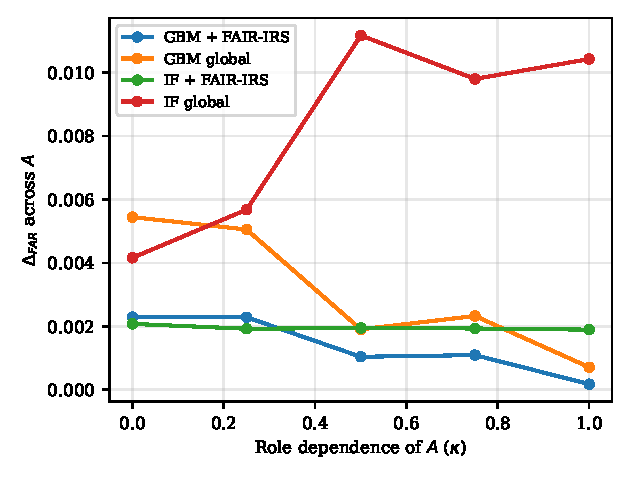
\includegraphics[width=0.95\columnwidth]{figures/kappa.pdf}
\caption{False-alert disparity across the semi-synthetic attribute $A$ as its dependence on role $\kappa$ grows (r4.2), for IF and GBM under the global policy and under FAIR-IRS with parity on $A$.}
\label{fig:s-kappa}
\end{figure}
\begin{figure}[!t]
\centering
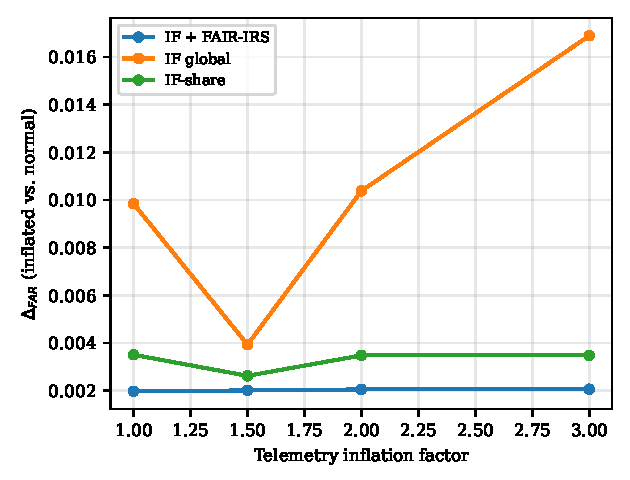
\includegraphics[width=0.95\columnwidth]{figures/injection.pdf}
\caption{False-alert disparity between employees with inflated and normal telemetry as the inflation factor $\mu$ grows (r4.2), for IF under the global policy, IF under FAIR-IRS, and exposure-normalized IF (B2, labeled IF-share).}
\label{fig:s-injection}
\end{figure}

\subsection{Synthetic Stress Tests}
Table~\ref{tab:s-stress} reports simulation S11 for every setting. Unless the factor is varied, the populations have five groups of $100$ employees, an activity gap of $0.5$, no dependence of risk on the group and a persistence of $0.5$. The global policy's disparity grows with the activity gap; cumulative allocation keeps it near $\delta$ in every setting, and the outcome-aware mode stays at or below $\delta$ even when group sizes are unequal or risk depends on the group. With high persistence, every policy detects fewer insiders, because persistent benign individuals crowd the top ranks.

\begin{table}[!t]
\caption{Synthetic Stress Tests for All Settings (Mean of Three Draws, $\delta$ = 0.002)\label{tab:s-stress}}
\centering
\resizebox{\columnwidth}{!}{%
\begin{tabular}{lcccccccc}
\toprule
Factor & Level & Policy & $\Delta_{\mathrm{FAR}}$ & $\rho_{\mathrm{FAR}}$ & Recall & Prec. & $\max F_i$ & Employees alerted \\
\midrule
activity gap & 0.0 & B0 global & 0.002 & 1.348 & 0.947 & 0.297 & 15.333 & 190.333 \\
activity gap & 0.0 & B8 daily parity & 0.002 & 1.232 & 0.933 & 0.254 & 14.333 & 200.000 \\
activity gap & 0.0 & B9 FA*IR bands & 0.002 & 1.342 & 0.953 & 0.294 & 15.667 & 190.000 \\
activity gap & 0.0 & B4 label-free & 0.002 & 1.255 & 0.953 & 0.278 & 15.000 & 197.333 \\
activity gap & 0.0 & B4c outcome-aware & 0.002 & 1.280 & 0.947 & 0.298 & 15.333 & 190.000 \\
activity gap & 0.25 & B0 global & 0.006 & 2.267 & 0.953 & 0.295 & 16.333 & 185.333 \\
activity gap & 0.25 & B8 daily parity & 0.002 & 1.232 & 0.933 & 0.254 & 14.333 & 200.000 \\
activity gap & 0.25 & B9 FA*IR bands & 0.006 & 2.246 & 0.953 & 0.293 & 16.667 & 184.333 \\
activity gap & 0.25 & B4 label-free & 0.002 & 1.320 & 0.953 & 0.273 & 15.000 & 194.000 \\
activity gap & 0.25 & B4c outcome-aware & 0.002 & 1.308 & 0.973 & 0.298 & 15.000 & 190.000 \\
activity gap & 0.5 & B0 global & 0.011 & 4.451 & 0.933 & 0.289 & 18.333 & 176.333 \\
activity gap & 0.5 & B8 daily parity & 0.002 & 1.232 & 0.933 & 0.254 & 14.333 & 200.000 \\
activity gap & 0.5 & B9 FA*IR bands & 0.010 & 4.271 & 0.933 & 0.288 & 19.000 & 176.333 \\
activity gap & 0.5 & B4 label-free & 0.002 & 1.302 & 0.967 & 0.270 & 16.000 & 193.333 \\
activity gap & 0.5 & B4c outcome-aware & 0.002 & 1.320 & 0.967 & 0.298 & 15.000 & 186.333 \\
activity gap & 1.0 & B0 global & 0.017 & 15.168 & 0.920 & 0.274 & 22.333 & 155.333 \\
activity gap & 1.0 & B8 daily parity & 0.002 & 1.232 & 0.933 & 0.254 & 14.333 & 200.000 \\
activity gap & 1.0 & B9 FA*IR bands & 0.016 & 13.988 & 0.920 & 0.275 & 21.333 & 157.000 \\
activity gap & 1.0 & B4 label-free & 0.002 & 1.321 & 0.960 & 0.266 & 15.000 & 193.667 \\
activity gap & 1.0 & B4c outcome-aware & 0.002 & 1.321 & 0.940 & 0.289 & 15.000 & 190.333 \\
group sizes & balanced & B0 global & 0.011 & 4.451 & 0.933 & 0.289 & 18.333 & 176.333 \\
group sizes & balanced & B8 daily parity & 0.002 & 1.232 & 0.933 & 0.254 & 14.333 & 200.000 \\
group sizes & balanced & B9 FA*IR bands & 0.010 & 4.271 & 0.933 & 0.288 & 19.000 & 176.333 \\
group sizes & balanced & B4 label-free & 0.002 & 1.302 & 0.967 & 0.270 & 16.000 & 193.333 \\
group sizes & balanced & B4c outcome-aware & 0.002 & 1.320 & 0.967 & 0.298 & 15.000 & 186.333 \\
group sizes & skewed & B0 global & 0.008 & 8.203 & 0.940 & 0.296 & 15.667 & 181.667 \\
group sizes & skewed & B8 daily parity & 0.010 & $\infty$ & 0.920 & 0.268 & 16.333 & 178.000 \\
group sizes & skewed & B9 FA*IR bands & 0.008 & 8.238 & 0.933 & 0.291 & 15.667 & 184.000 \\
group sizes & skewed & B4 label-free & 0.003 & 1.456 & 0.953 & 0.271 & 15.333 & 195.000 \\
group sizes & skewed & B4c outcome-aware & 0.002 & 1.337 & 0.947 & 0.295 & 16.333 & 189.667 \\
group sizes & one tiny group & B0 global & 0.010 & 8.695 & 0.940 & 0.291 & 16.667 & 178.667 \\
group sizes & one tiny group & B8 daily parity & 0.012 & $\infty$ & 0.900 & 0.260 & 20.333 & 186.333 \\
group sizes & one tiny group & B9 FA*IR bands & 0.009 & 6.068 & 0.940 & 0.290 & 16.667 & 181.667 \\
group sizes & one tiny group & B4 label-free & 0.003 & 1.484 & 0.940 & 0.267 & 15.333 & 188.333 \\
group sizes & one tiny group & B4c outcome-aware & 0.002 & 1.308 & 0.933 & 0.288 & 15.667 & 190.333 \\
risk ratio & 1.0 & B0 global & 0.011 & 4.451 & 0.933 & 0.289 & 18.333 & 176.333 \\
risk ratio & 1.0 & B8 daily parity & 0.002 & 1.232 & 0.933 & 0.254 & 14.333 & 200.000 \\
risk ratio & 1.0 & B9 FA*IR bands & 0.010 & 4.271 & 0.933 & 0.288 & 19.000 & 176.333 \\
risk ratio & 1.0 & B4 label-free & 0.002 & 1.302 & 0.967 & 0.270 & 16.000 & 193.333 \\
risk ratio & 1.0 & B4c outcome-aware & 0.002 & 1.320 & 0.967 & 0.298 & 15.000 & 186.333 \\
risk ratio & 3.0 & B0 global & 0.010 & 4.861 & 0.960 & 0.328 & 18.333 & 163.667 \\
risk ratio & 3.0 & B8 daily parity & 0.003 & 1.557 & 0.967 & 0.256 & 14.000 & 194.667 \\
risk ratio & 3.0 & B9 FA*IR bands & 0.009 & 4.301 & 0.967 & 0.327 & 18.000 & 164.667 \\
risk ratio & 3.0 & B4 label-free & 0.003 & 1.433 & 0.960 & 0.275 & 16.000 & 189.667 \\
risk ratio & 3.0 & B4c outcome-aware & 0.002 & 1.332 & 0.960 & 0.312 & 15.333 & 181.000 \\
risk ratio & 10.0 & B0 global & 0.010 & 4.585 & 0.980 & 0.340 & 16.333 & 158.667 \\
risk ratio & 10.0 & B8 daily parity & 0.004 & 1.993 & 0.927 & 0.255 & 12.000 & 194.333 \\
risk ratio & 10.0 & B9 FA*IR bands & 0.009 & 4.135 & 0.980 & 0.335 & 16.000 & 162.000 \\
risk ratio & 10.0 & B4 label-free & 0.003 & 1.661 & 0.947 & 0.274 & 13.667 & 192.000 \\
risk ratio & 10.0 & B4c outcome-aware & 0.002 & 1.337 & 0.973 & 0.320 & 13.000 & 180.667 \\
persistence & 0.0 & B0 global & 0.008 & 3.825 & 1.000 & 0.358 & 4.667 & 239.667 \\
persistence & 0.0 & B8 daily parity & 0.002 & 1.265 & 0.993 & 0.302 & 4.333 & 268.667 \\
persistence & 0.0 & B9 FA*IR bands & 0.008 & 3.602 & 1.000 & 0.355 & 4.667 & 242.667 \\
persistence & 0.0 & B4 label-free & 0.002 & 1.429 & 1.000 & 0.337 & 4.000 & 260.667 \\
persistence & 0.0 & B4c outcome-aware & 0.002 & 1.347 & 1.000 & 0.360 & 4.333 & 249.000 \\
persistence & 0.5 & B0 global & 0.011 & 4.451 & 0.933 & 0.289 & 18.333 & 176.333 \\
persistence & 0.5 & B8 daily parity & 0.002 & 1.232 & 0.933 & 0.254 & 14.333 & 200.000 \\
persistence & 0.5 & B9 FA*IR bands & 0.010 & 4.271 & 0.933 & 0.288 & 19.000 & 176.333 \\
persistence & 0.5 & B4 label-free & 0.002 & 1.302 & 0.967 & 0.270 & 16.000 & 193.333 \\
persistence & 0.5 & B4c outcome-aware & 0.002 & 1.320 & 0.967 & 0.298 & 15.000 & 186.333 \\
persistence & 1.0 & B0 global & 0.012 & 5.013 & 0.773 & 0.188 & 47.000 & 102.000 \\
persistence & 1.0 & B8 daily parity & 0.002 & 1.220 & 0.767 & 0.165 & 36.333 & 119.667 \\
persistence & 1.0 & B9 FA*IR bands & 0.012 & 4.788 & 0.767 & 0.187 & 47.000 & 104.000 \\
persistence & 1.0 & B4 label-free & 0.003 & 1.364 & 0.760 & 0.172 & 38.333 & 119.667 \\
persistence & 1.0 & B4c outcome-aware & 0.002 & 1.281 & 0.747 & 0.191 & 39.000 & 113.000 \\
\bottomrule
\end{tabular}}
\end{table}

\subsection{Robustness on r6.2}
Table~\ref{tab:s-robust} reports the five detectors on r6.2 under the global policy (B0) and both modes of FAIR-IRS (B4, B4c). The release contains three test insiders, so the ``Detected'' column is reported as a count. Both modes bring $\Delta_{\FAR}$ to $0.002$ for every detector. The burden findings replicate, and under GBM one benign employee is flagged on $249$ test days, whereas the detection results are too sparse to support conclusions.

\begin{table}[!t]
\caption{Robustness on r6.2 (Functional Units, $\delta$ = 0.002)\label{tab:s-robust}}
\centering
\resizebox{\columnwidth}{!}{%
\begin{tabular}{lcccccc}
\toprule
Detector & Policy & Detected & $\Delta_{\mathrm{FAR}}$ & $\rho_{\mathrm{FAR}}$ & Gini($F$) & $\max F_i$ \\
\midrule
IF & B0 & 1/3 & 0.047 & 9.865 & 0.975 & 145 \\
IF & B4 & 2/3 & 0.002 & 1.209 & 0.969 & 162 \\
IF & B4c & 2/3 & 0.002 & 1.209 & 0.969 & 162 \\
AE & B0 & 1/3 & 0.018 & 3.884 & 0.915 & 71 \\
AE & B4 & 2/3 & 0.002 & 1.227 & 0.912 & 78 \\
AE & B4c & 2/3 & 0.002 & 1.227 & 0.912 & 78 \\
LR & B0 & 0/3 & 0.026 & 92.142 & 0.899 & 95 \\
LR & B4 & 0/3 & 0.002 & 1.238 & 0.888 & 95 \\
LR & B4c & 0/3 & 0.002 & 1.238 & 0.888 & 95 \\
GBM & B0 & 0/3 & 0.012 & 3.049 & 0.989 & 249 \\
GBM & B4 & 0/3 & 0.002 & 1.218 & 0.988 & 248 \\
GBM & B4c & 0/3 & 0.002 & 1.218 & 0.988 & 248 \\
LSTM & B0 & 1/3 & 0.009 & 2.427 & 0.913 & 79 \\
LSTM & B4 & 1/3 & 0.002 & 1.227 & 0.912 & 80 \\
LSTM & B4c & 1/3 & 0.002 & 1.228 & 0.912 & 80 \\
\bottomrule
\end{tabular}}
\end{table}

\section{Security Experiments With Behavioral Relocation and Rescoring}
\label{sec:e-rev8}
This section gives the full results behind the main paper's attack results and Tables~S6 to S12 of the supplementary material: every timing attacker under behavioral relocation and rescoring (Tables~\ref{tab:e-l1-r42} and~\ref{tab:e-l1-r52}), every farming setting (Tables~\ref{tab:e-l3-r42} and~\ref{tab:e-l3-r52}), every verdict model (Tables~\ref{tab:e-l4-r42} and~\ref{tab:e-l4-r52}) and the social cost of every policy (Table~\ref{tab:e-l5}). The protocols are in Section~S-II-B of the supplementary material.

\begin{table*}[!t]
\caption{Timing Attacks With Behavioral Relocation and Rescoring, All Attackers (r4.2, $b=1\%$, $\delta=0.002$). Detected Under the Parity Rule P and the Global Policy G Without and With the Attack (Mean Over Draws); Excess Loss With the Mean of Per-Draw Paired Bootstrap Intervals and the Range Over Draws\label{tab:e-l1-r42}}
\centering
\scriptsize
\setlength{\tabcolsep}{3pt}
\begin{tabular}{lllccccccc}
\toprule
Det. & Parity rule & Attacker & P & G & P, attacked & G, attacked & Excess & 95\% & Range \\
\midrule
GBM & B4 label-free & knows allocation & 50 & 49 & 37.2 & 44.8 & 8.6 & [2.8, 14.8] & 5.0--11.0 \\
GBM & B4 label-free & observes colleagues & 50 & 49 & 44.0 & 46.2 & 3.2 & [-1.8, 8.4] & 3.0--4.0 \\
GBM & B4 label-free & reads reports & 50 & 49 & 46.6 & 47.4 & 1.8 & [-1.8, 5.8] & 1.0--5.0 \\
GBM & B4 label-free & estimates deficit & 50 & 49 & 44.4 & 48.2 & 4.8 & [-0.4, 10.2] & 3.0--8.0 \\
GBM & B4 label-free & random & 50 & 49 & 47.8 & 48.8 & 2.0 & [-2.0, 6.1] & 0.0--5.0 \\
GBM & B4c outcome-aware & knows allocation & 49 & 49 & 44.2 & 46.6 & 2.4 & [-2.0, 6.8] & 1.0--4.0 \\
GBM & B4c outcome-aware & observes colleagues & 49 & 49 & 45.8 & 47.0 & 1.2 & [-3.8, 6.4] & 1.0--2.0 \\
GBM & B4c outcome-aware & reads reports & 49 & 49 & 47.6 & 48.6 & 1.0 & [-2.4, 4.4] & -2.0--4.0 \\
GBM & B4c outcome-aware & estimates deficit & 49 & 49 & 44.0 & 44.6 & 0.6 & [-3.2, 4.2] & -1.0--2.0 \\
GBM & B4c outcome-aware & random & 49 & 49 & 47.5 & 48.8 & 1.3 & [-2.4, 5.2] & 0.0--4.0 \\
GBM & B4c outcome-aware, 7-day verdict delay & knows allocation & 49 & 49 & 33.6 & 41.6 & 8.0 & [1.8, 14.4] & 6.0--10.0 \\
GBM & B4c outcome-aware, 7-day verdict delay & observes colleagues & 49 & 49 & 45.0 & 47.2 & 2.2 & [-1.8, 6.4] & 2.0--3.0 \\
GBM & B4c outcome-aware, 7-day verdict delay & reads reports & 49 & 49 & 45.6 & 48.0 & 2.4 & [-2.0, 7.2] & 1.0--4.0 \\
GBM & B4c outcome-aware, 7-day verdict delay & estimates deficit & 49 & 49 & 43.8 & 46.6 & 2.8 & [-2.2, 7.6] & -1.0--5.0 \\
GBM & B4c outcome-aware, 7-day verdict delay & random & 49 & 49 & 47.8 & 48.8 & 1.0 & [-2.0, 4.5] & -2.0--4.0 \\
GBM & B11c deficit apportionment (outcome-aware) & knows allocation & 49 & 49 & 42.8 & 47.4 & 4.6 & [-1.4, 10.8] & 2.0--7.0 \\
GBM & B11c deficit apportionment (outcome-aware) & observes colleagues & 49 & 49 & 43.8 & 47.0 & 3.2 & [-2.6, 9.2] & 3.0--4.0 \\
GBM & B11c deficit apportionment (outcome-aware) & reads reports & 49 & 49 & 45.8 & 48.6 & 2.8 & [-2.0, 8.0] & 0.0--6.0 \\
GBM & B11c deficit apportionment (outcome-aware) & estimates deficit & 49 & 49 & 37.8 & 44.2 & 6.4 & [0.0, 12.8] & 4.0--8.0 \\
GBM & B11c deficit apportionment (outcome-aware) & random & 49 & 49 & 46.9 & 48.8 & 1.9 & [-3.1, 7.1] & 0.0--4.0 \\
LSTM & B4 label-free & knows allocation & 32 & 36 & 32.0 & 36.0 & 0.0 & [-4.8, 4.6] & -2.0--2.0 \\
LSTM & B4 label-free & observes colleagues & 32 & 36 & 30.0 & 35.0 & 1.0 & [-3.0, 5.0] & 1.0--1.0 \\
LSTM & B4 label-free & reads reports & 32 & 36 & 32.0 & 34.2 & -1.8 & [-5.6, 1.6] & -5.0--0.0 \\
LSTM & B4 label-free & estimates deficit & 32 & 36 & 29.8 & 34.6 & 0.8 & [-4.2, 5.6] & -1.0--4.0 \\
LSTM & B4 label-free & random & 32 & 36 & 33.5 & 35.3 & -2.2 & [-6.7, 1.9] & -5.0--2.0 \\
LSTM & B4c outcome-aware & knows allocation & 34 & 36 & 32.2 & 33.6 & -0.6 & [-5.8, 4.8] & -2.0--1.0 \\
LSTM & B4c outcome-aware & observes colleagues & 34 & 36 & 30.0 & 36.4 & 4.4 & [-2.2, 11.0] & 4.0--5.0 \\
LSTM & B4c outcome-aware & reads reports & 34 & 36 & 33.8 & 36.6 & 0.8 & [-3.0, 4.6] & -1.0--3.0 \\
LSTM & B4c outcome-aware & estimates deficit & 34 & 36 & 31.4 & 34.8 & 1.4 & [-2.4, 5.4] & 0.0--4.0 \\
LSTM & B4c outcome-aware & random & 34 & 36 & 33.7 & 35.3 & -0.4 & [-5.1, 4.2] & -4.0--3.0 \\
LSTM & B4c outcome-aware, 7-day verdict delay & knows allocation & 32 & 36 & 31.8 & 37.2 & 1.4 & [-4.2, 6.6] & 0.0--3.0 \\
LSTM & B4c outcome-aware, 7-day verdict delay & observes colleagues & 32 & 36 & 33.0 & 35.0 & -2.0 & [-6.0, 2.0] & -2.0---2.0 \\
LSTM & B4c outcome-aware, 7-day verdict delay & reads reports & 32 & 36 & 33.0 & 37.2 & 0.2 & [-3.4, 3.8] & -1.0--1.0 \\
LSTM & B4c outcome-aware, 7-day verdict delay & estimates deficit & 32 & 36 & 30.2 & 33.4 & -0.8 & [-4.8, 3.0] & -1.0--0.0 \\
LSTM & B4c outcome-aware, 7-day verdict delay & random & 32 & 36 & 34.6 & 35.3 & -3.3 & [-8.2, 1.1] & -7.0---1.0 \\
LSTM & B11c deficit apportionment (outcome-aware) & knows allocation & 32 & 36 & 31.6 & 34.2 & -1.4 & [-8.0, 5.0] & -4.0--0.0 \\
LSTM & B11c deficit apportionment (outcome-aware) & observes colleagues & 32 & 36 & 28.0 & 35.2 & 3.2 & [-3.0, 9.6] & 3.0--4.0 \\
LSTM & B11c deficit apportionment (outcome-aware) & reads reports & 32 & 36 & 34.0 & 36.4 & -1.6 & [-7.2, 4.4] & -5.0--1.0 \\
LSTM & B11c deficit apportionment (outcome-aware) & estimates deficit & 32 & 36 & 31.2 & 34.2 & -1.0 & [-7.8, 5.8] & -3.0--2.0 \\
LSTM & B11c deficit apportionment (outcome-aware) & random & 32 & 36 & 33.1 & 35.3 & -1.8 & [-7.9, 4.1] & -6.0--2.0 \\
AE & B4 label-free & knows allocation & 33 & 33 & 34.6 & 38.4 & 3.8 & [-1.6, 9.6] & 2.0--5.0 \\
AE & B4 label-free & observes colleagues & 33 & 33 & 31.0 & 29.0 & -2.0 & [-7.0, 3.0] & -2.0---2.0 \\
AE & B4 label-free & reads reports & 33 & 33 & 35.4 & 35.0 & -0.4 & [-5.2, 4.6] & -3.0--2.0 \\
AE & B4 label-free & estimates deficit & 33 & 33 & 28.2 & 33.2 & 5.0 & [0.0, 10.4] & 3.0--7.0 \\
AE & B4 label-free & random & 33 & 33 & 36.9 & 36.5 & -0.4 & [-5.6, 4.8] & -4.0--2.0 \\
AE & B4c outcome-aware & knows allocation & 33 & 33 & 32.8 & 35.6 & 2.8 & [-2.6, 8.6] & 0.0--5.0 \\
AE & B4c outcome-aware & observes colleagues & 33 & 33 & 34.0 & 34.0 & 0.0 & [-5.0, 5.0] & 0.0--0.0 \\
AE & B4c outcome-aware & reads reports & 33 & 33 & 35.4 & 36.0 & 0.6 & [-3.6, 5.0] & 0.0--1.0 \\
AE & B4c outcome-aware & estimates deficit & 33 & 33 & 35.8 & 38.2 & 2.4 & [-2.2, 7.2] & 0.0--5.0 \\
AE & B4c outcome-aware & random & 33 & 33 & 37.9 & 36.5 & -1.4 & [-5.7, 2.7] & -5.0--2.0 \\
AE & B4c outcome-aware, 7-day verdict delay & knows allocation & 32 & 33 & 28.6 & 32.6 & 3.0 & [-2.6, 8.6] & 1.0--5.0 \\
AE & B4c outcome-aware, 7-day verdict delay & observes colleagues & 32 & 33 & 36.0 & 40.0 & 3.0 & [-2.0, 8.0] & 3.0--3.0 \\
AE & B4c outcome-aware, 7-day verdict delay & reads reports & 32 & 33 & 35.2 & 35.2 & -1.0 & [-5.6, 3.8] & -3.0--1.0 \\
AE & B4c outcome-aware, 7-day verdict delay & estimates deficit & 32 & 33 & 36.2 & 39.2 & 2.0 & [-3.0, 7.2] & -2.0--7.0 \\
AE & B4c outcome-aware, 7-day verdict delay & random & 32 & 33 & 37.0 & 36.5 & -1.5 & [-6.4, 3.3] & -5.0--1.0 \\
AE & B11c deficit apportionment (outcome-aware) & knows allocation & 33 & 33 & 29.0 & 36.8 & 7.8 & [0.8, 15.0] & 4.0--11.0 \\
AE & B11c deficit apportionment (outcome-aware) & observes colleagues & 33 & 33 & 36.0 & 36.0 & 0.0 & [-5.0, 5.0] & 0.0--0.0 \\
AE & B11c deficit apportionment (outcome-aware) & reads reports & 33 & 33 & 37.6 & 36.8 & -0.8 & [-6.6, 5.0] & -2.0--1.0 \\
AE & B11c deficit apportionment (outcome-aware) & estimates deficit & 33 & 33 & 29.2 & 34.6 & 5.4 & [-1.4, 12.2] & 3.0--8.0 \\
AE & B11c deficit apportionment (outcome-aware) & random & 33 & 33 & 37.2 & 36.5 & -0.7 & [-6.1, 4.6] & -5.0--2.0 \\
\bottomrule
\end{tabular}
\end{table*}

\begin{table*}[!t]
\caption{Timing Attacks With Behavioral Relocation and Rescoring, All Attackers (r5.2, $b=1\%$, $\delta=0.002$). Detected Under the Parity Rule P and the Global Policy G Without and With the Attack (Mean Over Draws); Excess Loss With the Mean of Per-Draw Paired Bootstrap Intervals and the Range Over Draws\label{tab:e-l1-r52}}
\centering
\scriptsize
\setlength{\tabcolsep}{3pt}
\begin{tabular}{lllccccccc}
\toprule
Det. & Parity rule & Attacker & P & G & P, attacked & G, attacked & Excess & 95\% & Range \\
\midrule
GBM & B4 label-free & knows allocation & 72 & 75 & 62.2 & 73.4 & 8.2 & [2.0, 15.0] & 7.0--9.0 \\
GBM & B4 label-free & observes colleagues & 72 & 75 & 63.0 & 75.0 & 9.0 & [2.6, 16.0] & 9.0--9.0 \\
GBM & B4 label-free & reads reports & 72 & 75 & 66.4 & 71.4 & 2.0 & [-2.6, 6.6] & 1.0--3.0 \\
GBM & B4 label-free & estimates deficit & 72 & 75 & 61.0 & 69.8 & 5.8 & [0.4, 12.2] & 4.0--9.0 \\
GBM & B4 label-free & random & 72 & 75 & 70.9 & 74.7 & 0.8 & [-3.1, 4.6] & -1.0--3.0 \\
GBM & B4c outcome-aware & knows allocation & 71 & 75 & 63.6 & 70.4 & 2.8 & [-2.4, 8.2] & 0.0--5.0 \\
GBM & B4c outcome-aware & observes colleagues & 71 & 75 & 63.8 & 75.0 & 7.2 & [2.0, 13.2] & 7.0--8.0 \\
GBM & B4c outcome-aware & reads reports & 71 & 75 & 67.8 & 71.4 & -0.4 & [-4.4, 3.0] & -1.0--1.0 \\
GBM & B4c outcome-aware & estimates deficit & 71 & 75 & 63.8 & 70.0 & 2.2 & [-2.4, 7.4] & 1.0--4.0 \\
GBM & B4c outcome-aware & random & 71 & 75 & 70.2 & 74.7 & 0.5 & [-2.3, 3.4] & -1.0--4.0 \\
GBM & B4c outcome-aware, 7-day verdict delay & knows allocation & 72 & 75 & 55.0 & 66.0 & 8.0 & [2.0, 14.6] & 6.0--10.0 \\
GBM & B4c outcome-aware, 7-day verdict delay & observes colleagues & 72 & 75 & 66.0 & 74.0 & 5.0 & [-1.0, 11.0] & 5.0--5.0 \\
GBM & B4c outcome-aware, 7-day verdict delay & reads reports & 72 & 75 & 65.8 & 72.0 & 3.2 & [-1.2, 8.2] & 1.0--6.0 \\
GBM & B4c outcome-aware, 7-day verdict delay & estimates deficit & 72 & 75 & 63.2 & 73.4 & 7.2 & [2.4, 12.6] & 6.0--8.0 \\
GBM & B4c outcome-aware, 7-day verdict delay & random & 72 & 75 & 69.8 & 74.7 & 1.9 & [-1.3, 5.6] & 0.0--4.0 \\
GBM & B11c deficit apportionment (outcome-aware) & knows allocation & 71 & 75 & 68.8 & 74.0 & 1.2 & [-3.0, 5.6] & 0.0--2.0 \\
GBM & B11c deficit apportionment (outcome-aware) & observes colleagues & 71 & 75 & 56.0 & 67.0 & 7.0 & [-1.0, 15.8] & 7.0--7.0 \\
GBM & B11c deficit apportionment (outcome-aware) & reads reports & 71 & 75 & 66.6 & 72.0 & 1.4 & [-3.8, 7.0] & 0.0--4.0 \\
GBM & B11c deficit apportionment (outcome-aware) & estimates deficit & 71 & 75 & 60.4 & 69.6 & 5.2 & [-0.4, 11.6] & 4.0--7.0 \\
GBM & B11c deficit apportionment (outcome-aware) & random & 71 & 75 & 69.7 & 74.7 & 1.0 & [-3.0, 5.1] & -1.0--4.0 \\
LSTM & B4 label-free & knows allocation & 48 & 47 & 37.8 & 42.4 & 5.6 & [-1.2, 12.8] & 4.0--7.0 \\
LSTM & B4 label-free & observes colleagues & 48 & 47 & 35.0 & 44.0 & 10.0 & [5.0, 16.0] & 10.0--10.0 \\
LSTM & B4 label-free & reads reports & 48 & 47 & 38.8 & 40.4 & 2.6 & [-1.2, 7.0] & 1.0--5.0 \\
LSTM & B4 label-free & estimates deficit & 48 & 47 & 37.0 & 45.2 & 9.2 & [3.2, 15.2] & 7.0--13.0 \\
LSTM & B4 label-free & random & 48 & 47 & 43.2 & 43.9 & 1.7 & [-2.7, 6.2] & -2.0--4.0 \\
LSTM & B4c outcome-aware & knows allocation & 49 & 47 & 37.2 & 42.6 & 7.4 & [0.8, 14.2] & 6.0--9.0 \\
LSTM & B4c outcome-aware & observes colleagues & 49 & 47 & 37.0 & 44.0 & 9.0 & [3.6, 16.0] & 9.0--9.0 \\
LSTM & B4c outcome-aware & reads reports & 49 & 47 & 38.4 & 39.8 & 3.4 & [-1.2, 8.4] & 2.0--5.0 \\
LSTM & B4c outcome-aware & estimates deficit & 49 & 47 & 37.0 & 44.2 & 9.2 & [3.6, 15.8] & 4.0--14.0 \\
LSTM & B4c outcome-aware & random & 49 & 47 & 42.2 & 43.9 & 3.7 & [-1.2, 8.9] & 0.0--8.0 \\
LSTM & B4c outcome-aware, 7-day verdict delay & knows allocation & 48 & 47 & 39.4 & 43.0 & 4.6 & [-1.2, 10.6] & 3.0--6.0 \\
LSTM & B4c outcome-aware, 7-day verdict delay & observes colleagues & 48 & 47 & 39.0 & 45.0 & 7.0 & [2.4, 12.0] & 7.0--7.0 \\
LSTM & B4c outcome-aware, 7-day verdict delay & reads reports & 48 & 47 & 39.8 & 41.4 & 2.6 & [-1.8, 7.2] & 2.0--4.0 \\
LSTM & B4c outcome-aware, 7-day verdict delay & estimates deficit & 48 & 47 & 34.8 & 43.0 & 9.2 & [2.8, 16.4] & 5.0--13.0 \\
LSTM & B4c outcome-aware, 7-day verdict delay & random & 48 & 47 & 42.5 & 43.9 & 2.4 & [-2.0, 7.2] & 0.0--6.0 \\
LSTM & B11c deficit apportionment (outcome-aware) & knows allocation & 46 & 47 & 37.0 & 46.6 & 8.6 & [1.0, 16.6] & 6.0--11.0 \\
LSTM & B11c deficit apportionment (outcome-aware) & observes colleagues & 46 & 47 & 31.0 & 40.0 & 8.0 & [0.2, 16.0] & 8.0--8.0 \\
LSTM & B11c deficit apportionment (outcome-aware) & reads reports & 46 & 47 & 39.4 & 41.0 & 0.6 & [-6.0, 7.2] & -2.0--4.0 \\
LSTM & B11c deficit apportionment (outcome-aware) & estimates deficit & 46 & 47 & 36.4 & 42.0 & 4.6 & [-3.2, 12.2] & 3.0--6.0 \\
LSTM & B11c deficit apportionment (outcome-aware) & random & 46 & 47 & 41.3 & 43.9 & 1.6 & [-6.0, 9.3] & -4.0--7.0 \\
AE & B4 label-free & knows allocation & 58 & 61 & 54.0 & 61.8 & 4.8 & [-1.6, 11.6] & 3.0--8.0 \\
AE & B4 label-free & observes colleagues & 58 & 61 & 56.0 & 61.0 & 2.0 & [-5.0, 9.0] & 2.0--2.0 \\
AE & B4 label-free & reads reports & 58 & 61 & 57.4 & 61.4 & 1.0 & [-5.0, 7.4] & -1.0--2.0 \\
AE & B4 label-free & estimates deficit & 58 & 61 & 47.8 & 58.0 & 7.2 & [0.4, 14.4] & 3.0--10.0 \\
AE & B4 label-free & random & 58 & 61 & 58.8 & 61.0 & -0.8 & [-6.3, 4.7] & -4.0--2.0 \\
AE & B4c outcome-aware & knows allocation & 58 & 61 & 59.6 & 61.2 & -1.4 & [-6.2, 3.4] & -3.0--0.0 \\
AE & B4c outcome-aware & observes colleagues & 58 & 61 & 56.0 & 60.0 & 1.0 & [-4.0, 6.0] & 1.0--1.0 \\
AE & B4c outcome-aware & reads reports & 58 & 61 & 58.8 & 62.6 & 0.8 & [-4.8, 6.6] & -1.0--3.0 \\
AE & B4c outcome-aware & estimates deficit & 58 & 61 & 54.0 & 58.2 & 1.2 & [-5.2, 7.8] & -1.0--4.0 \\
AE & B4c outcome-aware & random & 58 & 61 & 58.3 & 61.0 & -0.3 & [-5.5, 4.7] & -4.0--4.0 \\
AE & B4c outcome-aware, 7-day verdict delay & knows allocation & 58 & 61 & 57.4 & 60.6 & 0.2 & [-6.0, 6.4] & -4.0--5.0 \\
AE & B4c outcome-aware, 7-day verdict delay & observes colleagues & 58 & 61 & 50.0 & 59.0 & 6.0 & [0.0, 12.0] & 6.0--6.0 \\
AE & B4c outcome-aware, 7-day verdict delay & reads reports & 58 & 61 & 58.6 & 62.6 & 1.0 & [-5.0, 7.0] & -1.0--3.0 \\
AE & B4c outcome-aware, 7-day verdict delay & estimates deficit & 58 & 61 & 51.8 & 56.6 & 1.8 & [-4.6, 8.4] & 0.0--5.0 \\
AE & B4c outcome-aware, 7-day verdict delay & random & 58 & 61 & 58.9 & 61.0 & -0.9 & [-6.4, 4.6] & -5.0--3.0 \\
AE & B11c deficit apportionment (outcome-aware) & knows allocation & 56 & 61 & 57.4 & 60.8 & -1.6 & [-6.4, 3.0] & -3.0---1.0 \\
AE & B11c deficit apportionment (outcome-aware) & observes colleagues & 56 & 61 & 55.0 & 61.0 & 1.0 & [-4.0, 6.0] & 1.0--1.0 \\
AE & B11c deficit apportionment (outcome-aware) & reads reports & 56 & 61 & 60.2 & 62.8 & -2.4 & [-7.8, 2.8] & -4.0---1.0 \\
AE & B11c deficit apportionment (outcome-aware) & estimates deficit & 56 & 61 & 55.4 & 61.2 & 0.8 & [-5.2, 6.6] & -2.0--5.0 \\
AE & B11c deficit apportionment (outcome-aware) & random & 56 & 61 & 58.8 & 61.0 & -2.8 & [-8.4, 2.6] & -8.0--2.0 \\
\bottomrule
\end{tabular}
\end{table*}

\begin{longtable}{lllllccccccc}
\caption{Realistic Discount Farming, All Settings (r4.2; Probes Capped at the Role's Benign 99th Percentile and Rescored; Mean of Three Draws When $p<1$). Det.: Detected Without Farming; Probed: Farmers With an Alerted Probe; Attack Det.: Attack Days Alerted; Exposed: a Probe Confirmed; Caught: Either\label{tab:e-l3-r42}}\\
\toprule
Det. & Knowl. & $n$ & $p$ & Policy & Det. & Probed & Attack det. & Exposed & Caught & Evaded & Gained \\
\midrule
\endfirsthead
\toprule
Det. & Knowl. & $n$ & $p$ & Policy & Det. & Probed & Attack det. & Exposed & Caught & Evaded & Gained \\
\midrule
\endhead
GBM & own & 1 & 1.0 & B0 global & 43 & 20.0 & 43.0 & 0.0 & 43.0 & 0.0 & 0.0 \\
GBM & own & 1 & 1.0 & B0 + scheduling & 44 & 21.0 & 44.0 & 0.0 & 44.0 & 0.0 & 0.0 \\
GBM & own & 1 & 1.0 & B0 + cooldown 30 days & 43 & 21.0 & 43.0 & 0.0 & 43.0 & 0.0 & 0.0 \\
GBM & own & 1 & 1.0 & B0 + cooldown 30 days, no override & 35 & 12.0 & 27.0 & 0.0 & 27.0 & 9.0 & 1.0 \\
GBM & own & 1 & 1.0 & B11c + cooldown 30 days & 40 & 19.0 & 40.0 & 0.0 & 40.0 & 0.0 & 0.0 \\
GBM & own & 3 & 1.0 & B0 global & 43 & 28.0 & 43.0 & 0.0 & 43.0 & 0.0 & 0.0 \\
GBM & own & 3 & 1.0 & B0 + scheduling & 44 & 29.0 & 44.0 & 0.0 & 44.0 & 1.0 & 1.0 \\
GBM & own & 3 & 1.0 & B0 + cooldown 30 days & 43 & 29.0 & 43.0 & 0.0 & 43.0 & 0.0 & 0.0 \\
GBM & own & 3 & 1.0 & B0 + cooldown 30 days, no override & 35 & 20.0 & 22.0 & 0.0 & 22.0 & 14.0 & 1.0 \\
GBM & own & 3 & 1.0 & B11c + cooldown 30 days & 40 & 29.0 & 39.0 & 0.0 & 39.0 & 1.0 & 0.0 \\
GBM & own & 5 & 1.0 & B0 global & 43 & 29.0 & 43.0 & 0.0 & 43.0 & 0.0 & 0.0 \\
GBM & own & 5 & 1.0 & B0 + scheduling & 44 & 29.0 & 45.0 & 0.0 & 45.0 & 0.0 & 1.0 \\
GBM & own & 5 & 1.0 & B0 + cooldown 30 days & 43 & 30.0 & 43.0 & 0.0 & 43.0 & 0.0 & 0.0 \\
GBM & own & 5 & 1.0 & B0 + cooldown 30 days, no override & 35 & 23.0 & 23.0 & 0.0 & 23.0 & 13.0 & 1.0 \\
GBM & own & 5 & 1.0 & B11c + cooldown 30 days & 40 & 32.0 & 40.0 & 0.0 & 40.0 & 0.0 & 0.0 \\
GBM & scenario & 1 & 1.0 & B0 global & 43 & 21.0 & 43.0 & 0.0 & 43.0 & 0.0 & 0.0 \\
GBM & scenario & 1 & 1.0 & B0 + scheduling & 44 & 23.0 & 43.0 & 0.0 & 43.0 & 1.0 & 0.0 \\
GBM & scenario & 1 & 1.0 & B0 + cooldown 30 days & 43 & 18.0 & 42.0 & 0.0 & 42.0 & 1.0 & 0.0 \\
GBM & scenario & 1 & 1.0 & B0 + cooldown 30 days, no override & 35 & 16.0 & 23.0 & 0.0 & 23.0 & 12.0 & 0.0 \\
GBM & scenario & 1 & 1.0 & B11c + cooldown 30 days & 40 & 18.0 & 39.0 & 0.0 & 39.0 & 1.0 & 0.0 \\
GBM & scenario & 3 & 1.0 & B0 global & 43 & 32.0 & 42.0 & 0.0 & 42.0 & 1.0 & 0.0 \\
GBM & scenario & 3 & 1.0 & B0 + scheduling & 44 & 33.0 & 43.0 & 0.0 & 43.0 & 1.0 & 0.0 \\
GBM & scenario & 3 & 1.0 & B0 + cooldown 30 days & 43 & 38.0 & 42.0 & 0.0 & 42.0 & 1.0 & 0.0 \\
GBM & scenario & 3 & 1.0 & B0 + cooldown 30 days, no override & 35 & 26.0 & 17.0 & 0.0 & 17.0 & 18.0 & 0.0 \\
GBM & scenario & 3 & 1.0 & B11c + cooldown 30 days & 40 & 33.0 & 40.0 & 0.0 & 40.0 & 0.0 & 0.0 \\
GBM & scenario & 5 & 1.0 & B0 global & 43 & 34.0 & 42.0 & 0.0 & 42.0 & 1.0 & 0.0 \\
GBM & scenario & 5 & 1.0 & B0 + scheduling & 44 & 35.0 & 43.0 & 0.0 & 43.0 & 1.0 & 0.0 \\
GBM & scenario & 5 & 1.0 & B0 + cooldown 30 days & 43 & 40.0 & 42.0 & 0.0 & 42.0 & 1.0 & 0.0 \\
GBM & scenario & 5 & 1.0 & B0 + cooldown 30 days, no override & 35 & 30.0 & 17.0 & 0.0 & 17.0 & 18.0 & 0.0 \\
GBM & scenario & 5 & 1.0 & B11c + cooldown 30 days & 40 & 35.0 & 40.0 & 0.0 & 40.0 & 0.0 & 0.0 \\
GBM & generic & 1 & 1.0 & B0 global & 43 & 20.0 & 43.0 & 0.0 & 43.0 & 0.0 & 0.0 \\
GBM & generic & 1 & 1.0 & B0 + scheduling & 44 & 22.0 & 44.0 & 0.0 & 44.0 & 0.0 & 0.0 \\
GBM & generic & 1 & 1.0 & B0 + cooldown 30 days & 43 & 23.0 & 42.0 & 0.0 & 42.0 & 1.0 & 0.0 \\
GBM & generic & 1 & 1.0 & B0 + cooldown 30 days, no override & 35 & 20.0 & 20.0 & 0.0 & 20.0 & 15.0 & 0.0 \\
GBM & generic & 1 & 1.0 & B11c + cooldown 30 days & 40 & 23.0 & 39.0 & 0.0 & 39.0 & 1.0 & 0.0 \\
GBM & generic & 3 & 1.0 & B0 global & 43 & 26.0 & 42.0 & 0.0 & 42.0 & 1.0 & 0.0 \\
GBM & generic & 3 & 1.0 & B0 + scheduling & 44 & 29.0 & 44.0 & 0.0 & 44.0 & 0.0 & 0.0 \\
GBM & generic & 3 & 1.0 & B0 + cooldown 30 days & 43 & 32.0 & 43.0 & 0.0 & 43.0 & 1.0 & 1.0 \\
GBM & generic & 3 & 1.0 & B0 + cooldown 30 days, no override & 35 & 25.0 & 17.0 & 0.0 & 17.0 & 18.0 & 0.0 \\
GBM & generic & 3 & 1.0 & B11c + cooldown 30 days & 40 & 28.0 & 40.0 & 0.0 & 40.0 & 2.0 & 2.0 \\
GBM & generic & 5 & 1.0 & B0 global & 43 & 29.0 & 42.0 & 0.0 & 42.0 & 1.0 & 0.0 \\
GBM & generic & 5 & 1.0 & B0 + scheduling & 44 & 33.0 & 44.0 & 0.0 & 44.0 & 0.0 & 0.0 \\
GBM & generic & 5 & 1.0 & B0 + cooldown 30 days & 43 & 33.0 & 43.0 & 0.0 & 43.0 & 1.0 & 1.0 \\
GBM & generic & 5 & 1.0 & B0 + cooldown 30 days, no override & 35 & 29.0 & 17.0 & 0.0 & 17.0 & 18.0 & 0.0 \\
GBM & generic & 5 & 1.0 & B11c + cooldown 30 days & 40 & 31.0 & 41.0 & 0.0 & 41.0 & 0.0 & 1.0 \\
GBM & own & 3 & 0.5 & B0 global & 43 & 28.0 & 43.0 & 22.0 & 43.7 & 0.0 & 0.7 \\
GBM & own & 3 & 0.5 & B0 + scheduling & 44 & 29.0 & 43.7 & 21.0 & 44.3 & 0.7 & 1.0 \\
GBM & own & 3 & 0.5 & B0 + cooldown 30 days & 43 & 30.0 & 43.3 & 20.0 & 43.3 & 0.0 & 0.3 \\
GBM & own & 3 & 0.5 & B0 + cooldown 30 days, no override & 35 & 19.7 & 24.7 & 10.0 & 30.0 & 6.7 & 1.7 \\
GBM & own & 3 & 0.5 & B11c + cooldown 30 days & 40 & 30.0 & 41.0 & 20.0 & 41.3 & 0.3 & 1.7 \\
GBM & own & 3 & 0.8 & B0 global & 43 & 28.0 & 43.0 & 12.7 & 43.3 & 0.0 & 0.3 \\
GBM & own & 3 & 0.8 & B0 + scheduling & 44 & 29.0 & 43.7 & 11.0 & 43.7 & 1.0 & 0.7 \\
GBM & own & 3 & 0.8 & B0 + cooldown 30 days & 43 & 29.7 & 43.3 & 9.3 & 43.3 & 0.0 & 0.3 \\
GBM & own & 3 & 0.8 & B0 + cooldown 30 days, no override & 35 & 20.0 & 23.3 & 4.3 & 25.0 & 11.7 & 1.7 \\
GBM & own & 3 & 0.8 & B11c + cooldown 30 days & 40 & 30.7 & 40.3 & 9.0 & 41.0 & 0.7 & 1.7 \\
GBM & scenario & 3 & 0.5 & B0 global & 43 & 32.0 & 42.0 & 22.7 & 43.0 & 1.0 & 1.0 \\
GBM & scenario & 3 & 0.5 & B0 + scheduling & 44 & 33.0 & 43.3 & 23.0 & 43.7 & 0.7 & 0.3 \\
GBM & scenario & 3 & 0.5 & B0 + cooldown 30 days & 43 & 36.7 & 42.7 & 23.3 & 43.7 & 0.7 & 1.3 \\
GBM & scenario & 3 & 0.5 & B0 + cooldown 30 days, no override & 35 & 25.7 & 23.3 & 12.3 & 28.0 & 9.7 & 2.7 \\
GBM & scenario & 3 & 0.5 & B11c + cooldown 30 days & 40 & 33.7 & 40.7 & 19.7 & 41.0 & 1.0 & 2.0 \\
GBM & scenario & 3 & 0.8 & B0 global & 43 & 32.0 & 42.0 & 12.0 & 42.3 & 1.0 & 0.3 \\
GBM & scenario & 3 & 0.8 & B0 + scheduling & 44 & 33.0 & 43.0 & 8.7 & 44.3 & 0.0 & 0.3 \\
GBM & scenario & 3 & 0.8 & B0 + cooldown 30 days & 43 & 37.7 & 42.7 & 10.0 & 43.3 & 1.0 & 1.3 \\
GBM & scenario & 3 & 0.8 & B0 + cooldown 30 days, no override & 35 & 25.7 & 18.0 & 6.7 & 23.0 & 13.0 & 1.0 \\
GBM & scenario & 3 & 0.8 & B11c + cooldown 30 days & 40 & 33.7 & 40.0 & 7.3 & 40.3 & 0.3 & 0.7 \\
GBM & generic & 3 & 0.5 & B0 global & 43 & 26.0 & 42.0 & 15.3 & 42.3 & 1.0 & 0.3 \\
GBM & generic & 3 & 0.5 & B0 + scheduling & 44 & 29.0 & 44.0 & 19.7 & 44.0 & 0.0 & 0.0 \\
GBM & generic & 3 & 0.5 & B0 + cooldown 30 days & 43 & 31.7 & 43.3 & 19.7 & 43.3 & 0.7 & 1.0 \\
GBM & generic & 3 & 0.5 & B0 + cooldown 30 days, no override & 35 & 25.0 & 24.7 & 12.7 & 29.3 & 7.7 & 2.0 \\
GBM & generic & 3 & 0.5 & B11c + cooldown 30 days & 40 & 29.3 & 40.3 & 19.3 & 40.7 & 1.3 & 2.0 \\
GBM & generic & 3 & 0.8 & B0 global & 43 & 26.0 & 42.0 & 9.0 & 42.0 & 1.0 & 0.0 \\
GBM & generic & 3 & 0.8 & B0 + scheduling & 44 & 29.0 & 44.0 & 7.3 & 44.0 & 0.0 & 0.0 \\
GBM & generic & 3 & 0.8 & B0 + cooldown 30 days & 43 & 32.0 & 43.0 & 10.0 & 43.0 & 1.0 & 1.0 \\
GBM & generic & 3 & 0.8 & B0 + cooldown 30 days, no override & 35 & 24.3 & 20.0 & 7.7 & 24.7 & 11.7 & 1.3 \\
GBM & generic & 3 & 0.8 & B11c + cooldown 30 days & 40 & 30.0 & 40.7 & 8.7 & 40.7 & 0.7 & 1.3 \\
AE & own & 1 & 1.0 & B0 global & 32 & 4.0 & 32.0 & 0.0 & 32.0 & 0.0 & 0.0 \\
AE & own & 1 & 1.0 & B0 + scheduling & 35 & 3.0 & 34.0 & 0.0 & 34.0 & 1.0 & 0.0 \\
AE & own & 1 & 1.0 & B0 + cooldown 30 days & 32 & 9.0 & 29.0 & 0.0 & 29.0 & 3.0 & 0.0 \\
AE & own & 1 & 1.0 & B0 + cooldown 30 days, no override & 24 & 7.0 & 20.0 & 0.0 & 20.0 & 4.0 & 0.0 \\
AE & own & 1 & 1.0 & B11c + cooldown 30 days & 31 & 7.0 & 29.0 & 0.0 & 29.0 & 2.0 & 0.0 \\
AE & own & 3 & 1.0 & B0 global & 32 & 9.0 & 32.0 & 0.0 & 32.0 & 0.0 & 0.0 \\
AE & own & 3 & 1.0 & B0 + scheduling & 35 & 10.0 & 35.0 & 0.0 & 35.0 & 1.0 & 1.0 \\
AE & own & 3 & 1.0 & B0 + cooldown 30 days & 32 & 19.0 & 28.0 & 0.0 & 28.0 & 4.0 & 0.0 \\
AE & own & 3 & 1.0 & B0 + cooldown 30 days, no override & 24 & 17.0 & 20.0 & 0.0 & 20.0 & 4.0 & 0.0 \\
AE & own & 3 & 1.0 & B11c + cooldown 30 days & 31 & 17.0 & 26.0 & 0.0 & 26.0 & 5.0 & 0.0 \\
AE & own & 5 & 1.0 & B0 global & 32 & 11.0 & 32.0 & 0.0 & 32.0 & 0.0 & 0.0 \\
AE & own & 5 & 1.0 & B0 + scheduling & 35 & 14.0 & 35.0 & 0.0 & 35.0 & 1.0 & 1.0 \\
AE & own & 5 & 1.0 & B0 + cooldown 30 days & 32 & 24.0 & 29.0 & 0.0 & 29.0 & 3.0 & 0.0 \\
AE & own & 5 & 1.0 & B0 + cooldown 30 days, no override & 24 & 18.0 & 20.0 & 0.0 & 20.0 & 4.0 & 0.0 \\
AE & own & 5 & 1.0 & B11c + cooldown 30 days & 31 & 21.0 & 27.0 & 0.0 & 27.0 & 5.0 & 1.0 \\
AE & scenario & 1 & 1.0 & B0 global & 32 & 3.0 & 32.0 & 0.0 & 32.0 & 0.0 & 0.0 \\
AE & scenario & 1 & 1.0 & B0 + scheduling & 35 & 3.0 & 35.0 & 0.0 & 35.0 & 0.0 & 0.0 \\
AE & scenario & 1 & 1.0 & B0 + cooldown 30 days & 32 & 8.0 & 29.0 & 0.0 & 29.0 & 3.0 & 0.0 \\
AE & scenario & 1 & 1.0 & B0 + cooldown 30 days, no override & 24 & 6.0 & 22.0 & 0.0 & 22.0 & 2.0 & 0.0 \\
AE & scenario & 1 & 1.0 & B11c + cooldown 30 days & 31 & 6.0 & 29.0 & 0.0 & 29.0 & 2.0 & 0.0 \\
AE & scenario & 3 & 1.0 & B0 global & 32 & 14.0 & 32.0 & 0.0 & 32.0 & 0.0 & 0.0 \\
AE & scenario & 3 & 1.0 & B0 + scheduling & 35 & 14.0 & 34.0 & 0.0 & 34.0 & 1.0 & 0.0 \\
AE & scenario & 3 & 1.0 & B0 + cooldown 30 days & 32 & 16.0 & 28.0 & 0.0 & 28.0 & 4.0 & 0.0 \\
AE & scenario & 3 & 1.0 & B0 + cooldown 30 days, no override & 24 & 15.0 & 22.0 & 0.0 & 22.0 & 2.0 & 0.0 \\
AE & scenario & 3 & 1.0 & B11c + cooldown 30 days & 31 & 15.0 & 27.0 & 0.0 & 27.0 & 7.0 & 3.0 \\
AE & scenario & 5 & 1.0 & B0 global & 32 & 16.0 & 32.0 & 0.0 & 32.0 & 0.0 & 0.0 \\
AE & scenario & 5 & 1.0 & B0 + scheduling & 35 & 18.0 & 34.0 & 0.0 & 34.0 & 1.0 & 0.0 \\
AE & scenario & 5 & 1.0 & B0 + cooldown 30 days & 32 & 24.0 & 29.0 & 0.0 & 29.0 & 3.0 & 0.0 \\
AE & scenario & 5 & 1.0 & B0 + cooldown 30 days, no override & 24 & 21.0 & 22.0 & 0.0 & 22.0 & 2.0 & 0.0 \\
AE & scenario & 5 & 1.0 & B11c + cooldown 30 days & 31 & 22.0 & 27.0 & 0.0 & 27.0 & 5.0 & 1.0 \\
AE & generic & 1 & 1.0 & B0 global & 32 & 3.0 & 32.0 & 0.0 & 32.0 & 0.0 & 0.0 \\
AE & generic & 1 & 1.0 & B0 + scheduling & 35 & 2.0 & 35.0 & 0.0 & 35.0 & 0.0 & 0.0 \\
AE & generic & 1 & 1.0 & B0 + cooldown 30 days & 32 & 7.0 & 29.0 & 0.0 & 29.0 & 3.0 & 0.0 \\
AE & generic & 1 & 1.0 & B0 + cooldown 30 days, no override & 24 & 6.0 & 22.0 & 0.0 & 22.0 & 2.0 & 0.0 \\
AE & generic & 1 & 1.0 & B11c + cooldown 30 days & 31 & 5.0 & 29.0 & 0.0 & 29.0 & 2.0 & 0.0 \\
AE & generic & 3 & 1.0 & B0 global & 32 & 7.0 & 32.0 & 0.0 & 32.0 & 0.0 & 0.0 \\
AE & generic & 3 & 1.0 & B0 + scheduling & 35 & 9.0 & 35.0 & 0.0 & 35.0 & 0.0 & 0.0 \\
AE & generic & 3 & 1.0 & B0 + cooldown 30 days & 32 & 15.0 & 29.0 & 0.0 & 29.0 & 3.0 & 0.0 \\
AE & generic & 3 & 1.0 & B0 + cooldown 30 days, no override & 24 & 14.0 & 23.0 & 0.0 & 23.0 & 2.0 & 1.0 \\
AE & generic & 3 & 1.0 & B11c + cooldown 30 days & 31 & 13.0 & 29.0 & 0.0 & 29.0 & 2.0 & 0.0 \\
AE & generic & 5 & 1.0 & B0 global & 32 & 10.0 & 32.0 & 0.0 & 32.0 & 0.0 & 0.0 \\
AE & generic & 5 & 1.0 & B0 + scheduling & 35 & 12.0 & 35.0 & 0.0 & 35.0 & 0.0 & 0.0 \\
AE & generic & 5 & 1.0 & B0 + cooldown 30 days & 32 & 26.0 & 29.0 & 0.0 & 29.0 & 3.0 & 0.0 \\
AE & generic & 5 & 1.0 & B0 + cooldown 30 days, no override & 24 & 23.0 & 22.0 & 0.0 & 22.0 & 2.0 & 0.0 \\
AE & generic & 5 & 1.0 & B11c + cooldown 30 days & 31 & 19.0 & 27.0 & 0.0 & 27.0 & 5.0 & 1.0 \\
AE & own & 3 & 0.5 & B0 global & 32 & 9.0 & 32.0 & 4.3 & 32.0 & 0.0 & 0.0 \\
AE & own & 3 & 0.5 & B0 + scheduling & 35 & 10.0 & 36.0 & 5.0 & 36.0 & 0.0 & 1.0 \\
AE & own & 3 & 0.5 & B0 + cooldown 30 days & 32 & 19.3 & 28.3 & 9.7 & 33.0 & 2.3 & 3.3 \\
AE & own & 3 & 0.5 & B0 + cooldown 30 days, no override & 24 & 16.0 & 22.7 & 6.0 & 25.3 & 3.3 & 4.7 \\
AE & own & 3 & 0.5 & B11c + cooldown 30 days & 31 & 17.7 & 28.7 & 9.0 & 33.0 & 3.0 & 5.0 \\
AE & own & 3 & 0.8 & B0 global & 32 & 9.0 & 32.0 & 2.7 & 32.0 & 0.0 & 0.0 \\
AE & own & 3 & 0.8 & B0 + scheduling & 35 & 10.0 & 35.0 & 3.3 & 35.3 & 0.7 & 1.0 \\
AE & own & 3 & 0.8 & B0 + cooldown 30 days & 32 & 19.0 & 27.7 & 2.0 & 29.3 & 3.7 & 1.0 \\
AE & own & 3 & 0.8 & B0 + cooldown 30 days, no override & 24 & 16.3 & 20.3 & 2.0 & 22.0 & 3.7 & 1.7 \\
AE & own & 3 & 0.8 & B11c + cooldown 30 days & 31 & 17.3 & 27.3 & 2.0 & 27.7 & 4.3 & 1.0 \\
AE & scenario & 3 & 0.5 & B0 global & 32 & 14.0 & 32.0 & 6.7 & 33.3 & 0.0 & 1.3 \\
AE & scenario & 3 & 0.5 & B0 + scheduling & 35 & 14.0 & 34.7 & 6.7 & 36.3 & 0.0 & 1.3 \\
AE & scenario & 3 & 0.5 & B0 + cooldown 30 days & 32 & 15.0 & 31.3 & 7.0 & 33.0 & 2.0 & 3.0 \\
AE & scenario & 3 & 0.5 & B0 + cooldown 30 days, no override & 24 & 15.0 & 24.3 & 4.7 & 26.0 & 2.0 & 4.0 \\
AE & scenario & 3 & 0.5 & B11c + cooldown 30 days & 31 & 16.3 & 27.3 & 7.0 & 30.0 & 4.0 & 3.0 \\
AE & scenario & 3 & 0.8 & B0 global & 32 & 14.0 & 32.0 & 4.0 & 33.7 & 0.0 & 1.7 \\
AE & scenario & 3 & 0.8 & B0 + scheduling & 35 & 14.0 & 34.3 & 2.7 & 35.0 & 0.7 & 0.7 \\
AE & scenario & 3 & 0.8 & B0 + cooldown 30 days & 32 & 16.0 & 28.0 & 1.7 & 28.3 & 3.7 & 0.0 \\
AE & scenario & 3 & 0.8 & B0 + cooldown 30 days, no override & 24 & 15.0 & 22.7 & 1.7 & 23.7 & 2.0 & 1.7 \\
AE & scenario & 3 & 0.8 & B11c + cooldown 30 days & 31 & 15.3 & 27.0 & 2.0 & 27.7 & 6.0 & 2.7 \\
AE & generic & 3 & 0.5 & B0 global & 32 & 7.0 & 32.0 & 3.0 & 32.0 & 0.0 & 0.0 \\
AE & generic & 3 & 0.5 & B0 + scheduling & 35 & 9.0 & 35.3 & 4.0 & 36.3 & 0.0 & 1.3 \\
AE & generic & 3 & 0.5 & B0 + cooldown 30 days & 32 & 16.7 & 31.3 & 10.7 & 34.0 & 2.0 & 4.0 \\
AE & generic & 3 & 0.5 & B0 + cooldown 30 days, no override & 24 & 15.0 & 27.3 & 7.7 & 29.0 & 1.3 & 6.3 \\
AE & generic & 3 & 0.5 & B11c + cooldown 30 days & 31 & 11.7 & 29.3 & 6.0 & 31.3 & 2.3 & 2.7 \\
AE & generic & 3 & 0.8 & B0 global & 32 & 7.0 & 32.0 & 2.7 & 32.0 & 0.0 & 0.0 \\
AE & generic & 3 & 0.8 & B0 + scheduling & 35 & 9.0 & 35.0 & 2.0 & 35.0 & 0.0 & 0.0 \\
AE & generic & 3 & 0.8 & B0 + cooldown 30 days & 32 & 15.0 & 29.7 & 2.0 & 30.3 & 2.3 & 0.7 \\
AE & generic & 3 & 0.8 & B0 + cooldown 30 days, no override & 24 & 14.3 & 23.0 & 2.0 & 25.0 & 1.7 & 2.7 \\
AE & generic & 3 & 0.8 & B11c + cooldown 30 days & 31 & 12.0 & 28.0 & 2.0 & 29.0 & 4.0 & 2.0 \\
LR & own & 1 & 1.0 & B0 global & 39 & 5.0 & 39.0 & 0.0 & 39.0 & 0.0 & 0.0 \\
LR & own & 1 & 1.0 & B0 + scheduling & 39 & 8.0 & 39.0 & 0.0 & 39.0 & 0.0 & 0.0 \\
LR & own & 1 & 1.0 & B0 + cooldown 30 days & 39 & 11.0 & 37.0 & 0.0 & 37.0 & 2.0 & 0.0 \\
LR & own & 1 & 1.0 & B0 + cooldown 30 days, no override & 28 & 12.0 & 19.0 & 0.0 & 19.0 & 9.0 & 0.0 \\
LR & own & 1 & 1.0 & B11c + cooldown 30 days & 39 & 9.0 & 37.0 & 0.0 & 37.0 & 2.0 & 0.0 \\
LR & own & 3 & 1.0 & B0 global & 39 & 14.0 & 38.0 & 0.0 & 38.0 & 1.0 & 0.0 \\
LR & own & 3 & 1.0 & B0 + scheduling & 39 & 22.0 & 39.0 & 0.0 & 39.0 & 0.0 & 0.0 \\
LR & own & 3 & 1.0 & B0 + cooldown 30 days & 39 & 21.0 & 38.0 & 0.0 & 38.0 & 2.0 & 1.0 \\
LR & own & 3 & 1.0 & B0 + cooldown 30 days, no override & 28 & 20.0 & 18.0 & 0.0 & 18.0 & 10.0 & 0.0 \\
LR & own & 3 & 1.0 & B11c + cooldown 30 days & 39 & 20.0 & 38.0 & 0.0 & 38.0 & 2.0 & 1.0 \\
LR & own & 5 & 1.0 & B0 global & 39 & 18.0 & 38.0 & 0.0 & 38.0 & 1.0 & 0.0 \\
LR & own & 5 & 1.0 & B0 + scheduling & 39 & 27.0 & 39.0 & 0.0 & 39.0 & 0.0 & 0.0 \\
LR & own & 5 & 1.0 & B0 + cooldown 30 days & 39 & 22.0 & 38.0 & 0.0 & 38.0 & 2.0 & 1.0 \\
LR & own & 5 & 1.0 & B0 + cooldown 30 days, no override & 28 & 22.0 & 18.0 & 0.0 & 18.0 & 10.0 & 0.0 \\
LR & own & 5 & 1.0 & B11c + cooldown 30 days & 39 & 24.0 & 37.0 & 0.0 & 37.0 & 2.0 & 0.0 \\
LR & scenario & 1 & 1.0 & B0 global & 39 & 7.0 & 39.0 & 0.0 & 39.0 & 0.0 & 0.0 \\
LR & scenario & 1 & 1.0 & B0 + scheduling & 39 & 17.0 & 39.0 & 0.0 & 39.0 & 0.0 & 0.0 \\
LR & scenario & 1 & 1.0 & B0 + cooldown 30 days & 39 & 11.0 & 37.0 & 0.0 & 37.0 & 2.0 & 0.0 \\
LR & scenario & 1 & 1.0 & B0 + cooldown 30 days, no override & 28 & 10.0 & 20.0 & 0.0 & 20.0 & 8.0 & 0.0 \\
LR & scenario & 1 & 1.0 & B11c + cooldown 30 days & 39 & 8.0 & 37.0 & 0.0 & 37.0 & 2.0 & 0.0 \\
LR & scenario & 3 & 1.0 & B0 global & 39 & 21.0 & 38.0 & 0.0 & 38.0 & 1.0 & 0.0 \\
LR & scenario & 3 & 1.0 & B0 + scheduling & 39 & 28.0 & 39.0 & 0.0 & 39.0 & 0.0 & 0.0 \\
LR & scenario & 3 & 1.0 & B0 + cooldown 30 days & 39 & 24.0 & 37.0 & 0.0 & 37.0 & 2.0 & 0.0 \\
LR & scenario & 3 & 1.0 & B0 + cooldown 30 days, no override & 28 & 21.0 & 18.0 & 0.0 & 18.0 & 10.0 & 0.0 \\
LR & scenario & 3 & 1.0 & B11c + cooldown 30 days & 39 & 23.0 & 36.0 & 0.0 & 36.0 & 3.0 & 0.0 \\
LR & scenario & 5 & 1.0 & B0 global & 39 & 22.0 & 38.0 & 0.0 & 38.0 & 1.0 & 0.0 \\
LR & scenario & 5 & 1.0 & B0 + scheduling & 39 & 29.0 & 39.0 & 0.0 & 39.0 & 0.0 & 0.0 \\
LR & scenario & 5 & 1.0 & B0 + cooldown 30 days & 39 & 26.0 & 37.0 & 0.0 & 37.0 & 2.0 & 0.0 \\
LR & scenario & 5 & 1.0 & B0 + cooldown 30 days, no override & 28 & 23.0 & 18.0 & 0.0 & 18.0 & 10.0 & 0.0 \\
LR & scenario & 5 & 1.0 & B11c + cooldown 30 days & 39 & 26.0 & 36.0 & 0.0 & 36.0 & 3.0 & 0.0 \\
LR & generic & 1 & 1.0 & B0 global & 39 & 25.0 & 39.0 & 0.0 & 39.0 & 0.0 & 0.0 \\
LR & generic & 1 & 1.0 & B0 + scheduling & 39 & 26.0 & 40.0 & 0.0 & 40.0 & 0.0 & 1.0 \\
LR & generic & 1 & 1.0 & B0 + cooldown 30 days & 39 & 19.0 & 34.0 & 0.0 & 34.0 & 5.0 & 0.0 \\
LR & generic & 1 & 1.0 & B0 + cooldown 30 days, no override & 28 & 16.0 & 16.0 & 0.0 & 16.0 & 12.0 & 0.0 \\
LR & generic & 1 & 1.0 & B11c + cooldown 30 days & 39 & 17.0 & 37.0 & 0.0 & 37.0 & 2.0 & 0.0 \\
LR & generic & 3 & 1.0 & B0 global & 39 & 38.0 & 38.0 & 0.0 & 38.0 & 1.0 & 0.0 \\
LR & generic & 3 & 1.0 & B0 + scheduling & 39 & 39.0 & 40.0 & 0.0 & 40.0 & 0.0 & 1.0 \\
LR & generic & 3 & 1.0 & B0 + cooldown 30 days & 39 & 33.0 & 35.0 & 0.0 & 35.0 & 4.0 & 0.0 \\
LR & generic & 3 & 1.0 & B0 + cooldown 30 days, no override & 28 & 24.0 & 16.0 & 0.0 & 16.0 & 12.0 & 0.0 \\
LR & generic & 3 & 1.0 & B11c + cooldown 30 days & 39 & 31.0 & 36.0 & 0.0 & 36.0 & 3.0 & 0.0 \\
LR & generic & 5 & 1.0 & B0 global & 39 & 38.0 & 38.0 & 0.0 & 38.0 & 1.0 & 0.0 \\
LR & generic & 5 & 1.0 & B0 + scheduling & 39 & 41.0 & 40.0 & 0.0 & 40.0 & 0.0 & 1.0 \\
LR & generic & 5 & 1.0 & B0 + cooldown 30 days & 39 & 35.0 & 34.0 & 0.0 & 34.0 & 5.0 & 0.0 \\
LR & generic & 5 & 1.0 & B0 + cooldown 30 days, no override & 28 & 27.0 & 16.0 & 0.0 & 16.0 & 12.0 & 0.0 \\
LR & generic & 5 & 1.0 & B11c + cooldown 30 days & 39 & 36.0 & 35.0 & 0.0 & 35.0 & 4.0 & 0.0 \\
LR & own & 3 & 0.5 & B0 global & 39 & 14.0 & 38.0 & 9.0 & 39.0 & 1.0 & 1.0 \\
LR & own & 3 & 0.5 & B0 + scheduling & 39 & 22.0 & 39.0 & 11.7 & 41.0 & 0.0 & 2.0 \\
LR & own & 3 & 0.5 & B0 + cooldown 30 days & 39 & 22.0 & 38.3 & 13.3 & 38.7 & 1.3 & 1.0 \\
LR & own & 3 & 0.5 & B0 + cooldown 30 days, no override & 28 & 20.3 & 21.7 & 8.0 & 25.0 & 5.7 & 2.7 \\
LR & own & 3 & 0.5 & B11c + cooldown 30 days & 39 & 22.3 & 38.0 & 8.3 & 38.3 & 1.0 & 0.3 \\
LR & own & 3 & 0.8 & B0 global & 39 & 14.0 & 38.0 & 4.3 & 38.0 & 1.0 & 0.0 \\
LR & own & 3 & 0.8 & B0 + scheduling & 39 & 22.0 & 39.0 & 4.7 & 39.0 & 0.0 & 0.0 \\
LR & own & 3 & 0.8 & B0 + cooldown 30 days & 39 & 21.0 & 38.3 & 2.3 & 38.3 & 1.7 & 1.0 \\
LR & own & 3 & 0.8 & B0 + cooldown 30 days, no override & 28 & 20.0 & 19.0 & 3.3 & 21.0 & 8.0 & 1.0 \\
LR & own & 3 & 0.8 & B11c + cooldown 30 days & 39 & 21.3 & 37.3 & 2.7 & 37.3 & 2.0 & 0.3 \\
LR & scenario & 3 & 0.5 & B0 global & 39 & 21.0 & 38.0 & 13.7 & 39.3 & 0.7 & 1.0 \\
LR & scenario & 3 & 0.5 & B0 + scheduling & 39 & 28.0 & 39.0 & 15.0 & 40.0 & 0.0 & 1.0 \\
LR & scenario & 3 & 0.5 & B0 + cooldown 30 days & 39 & 24.7 & 38.3 & 12.3 & 38.7 & 1.0 & 0.7 \\
LR & scenario & 3 & 0.5 & B0 + cooldown 30 days, no override & 28 & 21.0 & 22.0 & 8.7 & 25.0 & 5.7 & 2.7 \\
LR & scenario & 3 & 0.5 & B11c + cooldown 30 days & 39 & 22.7 & 36.0 & 12.3 & 36.7 & 2.7 & 0.3 \\
LR & scenario & 3 & 0.8 & B0 global & 39 & 21.0 & 38.0 & 6.7 & 38.3 & 1.0 & 0.3 \\
LR & scenario & 3 & 0.8 & B0 + scheduling & 39 & 28.0 & 39.0 & 4.7 & 39.3 & 0.0 & 0.3 \\
LR & scenario & 3 & 0.8 & B0 + cooldown 30 days & 39 & 24.3 & 37.7 & 5.7 & 37.7 & 1.7 & 0.3 \\
LR & scenario & 3 & 0.8 & B0 + cooldown 30 days, no override & 28 & 21.0 & 20.3 & 5.7 & 22.7 & 7.3 & 2.0 \\
LR & scenario & 3 & 0.8 & B11c + cooldown 30 days & 39 & 22.7 & 37.3 & 4.7 & 37.7 & 2.3 & 1.0 \\
LR & generic & 3 & 0.5 & B0 global & 39 & 38.0 & 38.0 & 27.0 & 41.0 & 1.0 & 3.0 \\
LR & generic & 3 & 0.5 & B0 + scheduling & 39 & 38.7 & 40.0 & 24.7 & 42.7 & 0.0 & 3.7 \\
LR & generic & 3 & 0.5 & B0 + cooldown 30 days & 39 & 33.3 & 35.7 & 20.3 & 38.0 & 2.0 & 1.0 \\
LR & generic & 3 & 0.5 & B0 + cooldown 30 days, no override & 28 & 25.7 & 19.3 & 14.3 & 27.7 & 5.0 & 4.7 \\
LR & generic & 3 & 0.5 & B11c + cooldown 30 days & 39 & 30.7 & 36.7 & 15.7 & 39.0 & 1.7 & 1.7 \\
LR & generic & 3 & 0.8 & B0 global & 39 & 38.0 & 38.0 & 15.0 & 39.3 & 1.0 & 1.3 \\
LR & generic & 3 & 0.8 & B0 + scheduling & 39 & 38.7 & 40.0 & 11.0 & 41.0 & 0.0 & 2.0 \\
LR & generic & 3 & 0.8 & B0 + cooldown 30 days & 39 & 33.0 & 35.0 & 9.3 & 36.7 & 2.7 & 0.3 \\
LR & generic & 3 & 0.8 & B0 + cooldown 30 days, no override & 28 & 25.3 & 15.0 & 4.0 & 18.3 & 10.7 & 1.0 \\
LR & generic & 3 & 0.8 & B11c + cooldown 30 days & 39 & 31.7 & 36.0 & 7.7 & 37.7 & 2.7 & 1.3 \\
IF & own & 1 & 1.0 & B0 global & 8 & 5.0 & 8.0 & 0.0 & 8.0 & 0.0 & 0.0 \\
IF & own & 1 & 1.0 & B0 + scheduling & 14 & 6.0 & 14.0 & 0.0 & 14.0 & 0.0 & 0.0 \\
IF & own & 1 & 1.0 & B0 + cooldown 30 days & 21 & 4.0 & 21.0 & 0.0 & 21.0 & 0.0 & 0.0 \\
IF & own & 1 & 1.0 & B0 + cooldown 30 days, no override & 21 & 5.0 & 20.0 & 0.0 & 20.0 & 1.0 & 0.0 \\
IF & own & 1 & 1.0 & B11c + cooldown 30 days & 22 & 5.0 & 22.0 & 0.0 & 22.0 & 1.0 & 1.0 \\
IF & own & 3 & 1.0 & B0 global & 8 & 10.0 & 8.0 & 0.0 & 8.0 & 0.0 & 0.0 \\
IF & own & 3 & 1.0 & B0 + scheduling & 14 & 14.0 & 14.0 & 0.0 & 14.0 & 0.0 & 0.0 \\
IF & own & 3 & 1.0 & B0 + cooldown 30 days & 21 & 14.0 & 21.0 & 0.0 & 21.0 & 0.0 & 0.0 \\
IF & own & 3 & 1.0 & B0 + cooldown 30 days, no override & 21 & 16.0 & 19.0 & 0.0 & 19.0 & 2.0 & 0.0 \\
IF & own & 3 & 1.0 & B11c + cooldown 30 days & 22 & 13.0 & 20.0 & 0.0 & 20.0 & 2.0 & 0.0 \\
IF & own & 5 & 1.0 & B0 global & 8 & 13.0 & 8.0 & 0.0 & 8.0 & 0.0 & 0.0 \\
IF & own & 5 & 1.0 & B0 + scheduling & 14 & 17.0 & 14.0 & 0.0 & 14.0 & 0.0 & 0.0 \\
IF & own & 5 & 1.0 & B0 + cooldown 30 days & 21 & 19.0 & 21.0 & 0.0 & 21.0 & 0.0 & 0.0 \\
IF & own & 5 & 1.0 & B0 + cooldown 30 days, no override & 21 & 20.0 & 19.0 & 0.0 & 19.0 & 2.0 & 0.0 \\
IF & own & 5 & 1.0 & B11c + cooldown 30 days & 22 & 17.0 & 20.0 & 0.0 & 20.0 & 2.0 & 0.0 \\
IF & scenario & 1 & 1.0 & B0 global & 8 & 5.0 & 8.0 & 0.0 & 8.0 & 0.0 & 0.0 \\
IF & scenario & 1 & 1.0 & B0 + scheduling & 14 & 8.0 & 13.0 & 0.0 & 13.0 & 1.0 & 0.0 \\
IF & scenario & 1 & 1.0 & B0 + cooldown 30 days & 21 & 8.0 & 20.0 & 0.0 & 20.0 & 1.0 & 0.0 \\
IF & scenario & 1 & 1.0 & B0 + cooldown 30 days, no override & 21 & 6.0 & 20.0 & 0.0 & 20.0 & 1.0 & 0.0 \\
IF & scenario & 1 & 1.0 & B11c + cooldown 30 days & 22 & 7.0 & 20.0 & 0.0 & 20.0 & 2.0 & 0.0 \\
IF & scenario & 3 & 1.0 & B0 global & 8 & 11.0 & 8.0 & 0.0 & 8.0 & 0.0 & 0.0 \\
IF & scenario & 3 & 1.0 & B0 + scheduling & 14 & 17.0 & 12.0 & 0.0 & 12.0 & 2.0 & 0.0 \\
IF & scenario & 3 & 1.0 & B0 + cooldown 30 days & 21 & 18.0 & 19.0 & 0.0 & 19.0 & 2.0 & 0.0 \\
IF & scenario & 3 & 1.0 & B0 + cooldown 30 days, no override & 21 & 17.0 & 19.0 & 0.0 & 19.0 & 2.0 & 0.0 \\
IF & scenario & 3 & 1.0 & B11c + cooldown 30 days & 22 & 14.0 & 21.0 & 0.0 & 21.0 & 1.0 & 0.0 \\
IF & scenario & 5 & 1.0 & B0 global & 8 & 14.0 & 8.0 & 0.0 & 8.0 & 0.0 & 0.0 \\
IF & scenario & 5 & 1.0 & B0 + scheduling & 14 & 20.0 & 12.0 & 0.0 & 12.0 & 2.0 & 0.0 \\
IF & scenario & 5 & 1.0 & B0 + cooldown 30 days & 21 & 22.0 & 19.0 & 0.0 & 19.0 & 2.0 & 0.0 \\
IF & scenario & 5 & 1.0 & B0 + cooldown 30 days, no override & 21 & 21.0 & 20.0 & 0.0 & 20.0 & 1.0 & 0.0 \\
IF & scenario & 5 & 1.0 & B11c + cooldown 30 days & 22 & 19.0 & 20.0 & 0.0 & 20.0 & 2.0 & 0.0 \\
IF & generic & 1 & 1.0 & B0 global & 8 & 5.0 & 8.0 & 0.0 & 8.0 & 0.0 & 0.0 \\
IF & generic & 1 & 1.0 & B0 + scheduling & 14 & 8.0 & 14.0 & 0.0 & 14.0 & 0.0 & 0.0 \\
IF & generic & 1 & 1.0 & B0 + cooldown 30 days & 21 & 13.0 & 18.0 & 0.0 & 18.0 & 3.0 & 0.0 \\
IF & generic & 1 & 1.0 & B0 + cooldown 30 days, no override & 21 & 9.0 & 18.0 & 0.0 & 18.0 & 3.0 & 0.0 \\
IF & generic & 1 & 1.0 & B11c + cooldown 30 days & 22 & 7.0 & 20.0 & 0.0 & 20.0 & 2.0 & 0.0 \\
IF & generic & 3 & 1.0 & B0 global & 8 & 9.0 & 8.0 & 0.0 & 8.0 & 0.0 & 0.0 \\
IF & generic & 3 & 1.0 & B0 + scheduling & 14 & 18.0 & 14.0 & 0.0 & 14.0 & 0.0 & 0.0 \\
IF & generic & 3 & 1.0 & B0 + cooldown 30 days & 21 & 21.0 & 18.0 & 0.0 & 18.0 & 3.0 & 0.0 \\
IF & generic & 3 & 1.0 & B0 + cooldown 30 days, no override & 21 & 21.0 & 17.0 & 0.0 & 17.0 & 4.0 & 0.0 \\
IF & generic & 3 & 1.0 & B11c + cooldown 30 days & 22 & 15.0 & 17.0 & 0.0 & 17.0 & 5.0 & 0.0 \\
IF & generic & 5 & 1.0 & B0 global & 8 & 12.0 & 8.0 & 0.0 & 8.0 & 0.0 & 0.0 \\
IF & generic & 5 & 1.0 & B0 + scheduling & 14 & 24.0 & 14.0 & 0.0 & 14.0 & 0.0 & 0.0 \\
IF & generic & 5 & 1.0 & B0 + cooldown 30 days & 21 & 25.0 & 18.0 & 0.0 & 18.0 & 3.0 & 0.0 \\
IF & generic & 5 & 1.0 & B0 + cooldown 30 days, no override & 21 & 23.0 & 17.0 & 0.0 & 17.0 & 4.0 & 0.0 \\
IF & generic & 5 & 1.0 & B11c + cooldown 30 days & 22 & 19.0 & 19.0 & 0.0 & 19.0 & 3.0 & 0.0 \\
IF & own & 3 & 0.5 & B0 global & 8 & 10.0 & 8.0 & 7.0 & 11.7 & 0.0 & 3.7 \\
IF & own & 3 & 0.5 & B0 + scheduling & 14 & 14.0 & 14.0 & 6.7 & 18.0 & 0.0 & 4.0 \\
IF & own & 3 & 0.5 & B0 + cooldown 30 days & 21 & 14.0 & 23.3 & 6.3 & 26.3 & 0.0 & 5.3 \\
IF & own & 3 & 0.5 & B0 + cooldown 30 days, no override & 21 & 15.7 & 22.7 & 10.0 & 27.7 & 0.0 & 6.7 \\
IF & own & 3 & 0.5 & B11c + cooldown 30 days & 22 & 13.7 & 21.3 & 5.7 & 24.3 & 2.3 & 4.7 \\
IF & own & 3 & 0.8 & B0 global & 8 & 10.0 & 8.0 & 3.3 & 9.3 & 0.0 & 1.3 \\
IF & own & 3 & 0.8 & B0 + scheduling & 14 & 14.0 & 14.0 & 4.3 & 17.0 & 0.0 & 3.0 \\
IF & own & 3 & 0.8 & B0 + cooldown 30 days & 21 & 14.0 & 21.7 & 2.3 & 23.3 & 0.0 & 2.3 \\
IF & own & 3 & 0.8 & B0 + cooldown 30 days, no override & 21 & 16.0 & 19.7 & 3.3 & 22.0 & 1.0 & 2.0 \\
IF & own & 3 & 0.8 & B11c + cooldown 30 days & 22 & 13.3 & 21.0 & 3.0 & 22.3 & 2.0 & 2.3 \\
IF & scenario & 3 & 0.5 & B0 global & 8 & 11.0 & 8.0 & 6.3 & 12.3 & 0.0 & 4.3 \\
IF & scenario & 3 & 0.5 & B0 + scheduling & 14 & 17.0 & 12.3 & 9.7 & 18.3 & 0.7 & 5.0 \\
IF & scenario & 3 & 0.5 & B0 + cooldown 30 days & 21 & 19.3 & 21.7 & 11.3 & 26.7 & 1.7 & 7.3 \\
IF & scenario & 3 & 0.5 & B0 + cooldown 30 days, no override & 21 & 17.3 & 21.3 & 10.0 & 26.7 & 0.7 & 6.3 \\
IF & scenario & 3 & 0.5 & B11c + cooldown 30 days & 22 & 14.3 & 22.0 & 9.0 & 28.0 & 1.3 & 7.3 \\
IF & scenario & 3 & 0.8 & B0 global & 8 & 11.0 & 8.0 & 4.0 & 10.3 & 0.0 & 2.3 \\
IF & scenario & 3 & 0.8 & B0 + scheduling & 14 & 17.0 & 12.3 & 6.0 & 16.0 & 1.0 & 3.0 \\
IF & scenario & 3 & 0.8 & B0 + cooldown 30 days & 21 & 18.0 & 19.7 & 3.7 & 22.0 & 2.0 & 3.0 \\
IF & scenario & 3 & 0.8 & B0 + cooldown 30 days, no override & 21 & 17.0 & 20.0 & 4.3 & 22.0 & 1.7 & 2.7 \\
IF & scenario & 3 & 0.8 & B11c + cooldown 30 days & 22 & 15.0 & 21.7 & 3.7 & 25.0 & 1.0 & 4.0 \\
IF & generic & 3 & 0.5 & B0 global & 8 & 9.0 & 8.0 & 4.7 & 10.3 & 0.0 & 2.3 \\
IF & generic & 3 & 0.5 & B0 + scheduling & 14 & 18.7 & 13.3 & 10.3 & 19.7 & 0.7 & 6.3 \\
IF & generic & 3 & 0.5 & B0 + cooldown 30 days & 21 & 21.7 & 21.3 & 13.0 & 27.0 & 1.7 & 7.7 \\
IF & generic & 3 & 0.5 & B0 + cooldown 30 days, no override & 21 & 21.3 & 18.3 & 9.0 & 23.7 & 2.7 & 5.3 \\
IF & generic & 3 & 0.5 & B11c + cooldown 30 days & 22 & 17.3 & 20.7 & 9.0 & 27.0 & 2.3 & 7.3 \\
IF & generic & 3 & 0.8 & B0 global & 8 & 9.0 & 8.0 & 2.7 & 9.0 & 0.0 & 1.0 \\
IF & generic & 3 & 0.8 & B0 + scheduling & 14 & 18.3 & 13.7 & 5.0 & 16.3 & 0.3 & 2.7 \\
IF & generic & 3 & 0.8 & B0 + cooldown 30 days & 21 & 22.0 & 19.0 & 4.7 & 21.3 & 2.0 & 2.3 \\
IF & generic & 3 & 0.8 & B0 + cooldown 30 days, no override & 21 & 21.0 & 17.3 & 5.0 & 21.0 & 3.7 & 3.7 \\
IF & generic & 3 & 0.8 & B11c + cooldown 30 days & 22 & 15.3 & 18.0 & 2.3 & 20.3 & 4.0 & 2.3 \\
\bottomrule
\end{longtable}

\begin{longtable}{lllllccccccc}
\caption{Realistic Discount Farming, All Settings (r5.2; Probes Capped at the Role's Benign 99th Percentile and Rescored; Mean of Three Draws When $p<1$). Det.: Detected Without Farming; Probed: Farmers With an Alerted Probe; Attack Det.: Attack Days Alerted; Exposed: a Probe Confirmed; Caught: Either\label{tab:e-l3-r52}}\\
\toprule
Det. & Knowl. & $n$ & $p$ & Policy & Det. & Probed & Attack det. & Exposed & Caught & Evaded & Gained \\
\midrule
\endfirsthead
\toprule
Det. & Knowl. & $n$ & $p$ & Policy & Det. & Probed & Attack det. & Exposed & Caught & Evaded & Gained \\
\midrule
\endhead
GBM & own & 1 & 1.0 & B0 global & 72 & 51.0 & 72.0 & 0.0 & 72.0 & 0.0 & 0.0 \\
GBM & own & 1 & 1.0 & B0 + scheduling & 72 & 55.0 & 71.0 & 0.0 & 71.0 & 1.0 & 0.0 \\
GBM & own & 1 & 1.0 & B0 + cooldown 30 days & 72 & 53.0 & 67.0 & 0.0 & 67.0 & 5.0 & 0.0 \\
GBM & own & 1 & 1.0 & B0 + cooldown 30 days, no override & 58 & 40.0 & 43.0 & 0.0 & 43.0 & 15.0 & 0.0 \\
GBM & own & 1 & 1.0 & B11c + cooldown 30 days & 67 & 48.0 & 65.0 & 0.0 & 65.0 & 2.0 & 0.0 \\
GBM & own & 3 & 1.0 & B0 global & 72 & 61.0 & 72.0 & 0.0 & 72.0 & 0.0 & 0.0 \\
GBM & own & 3 & 1.0 & B0 + scheduling & 72 & 63.0 & 71.0 & 0.0 & 71.0 & 1.0 & 0.0 \\
GBM & own & 3 & 1.0 & B0 + cooldown 30 days & 72 & 67.0 & 67.0 & 0.0 & 67.0 & 5.0 & 0.0 \\
GBM & own & 3 & 1.0 & B0 + cooldown 30 days, no override & 58 & 48.0 & 44.0 & 0.0 & 44.0 & 14.0 & 0.0 \\
GBM & own & 3 & 1.0 & B11c + cooldown 30 days & 67 & 64.0 & 65.0 & 0.0 & 65.0 & 3.0 & 1.0 \\
GBM & own & 5 & 1.0 & B0 global & 72 & 63.0 & 72.0 & 0.0 & 72.0 & 0.0 & 0.0 \\
GBM & own & 5 & 1.0 & B0 + scheduling & 72 & 66.0 & 71.0 & 0.0 & 71.0 & 1.0 & 0.0 \\
GBM & own & 5 & 1.0 & B0 + cooldown 30 days & 72 & 69.0 & 66.0 & 0.0 & 66.0 & 6.0 & 0.0 \\
GBM & own & 5 & 1.0 & B0 + cooldown 30 days, no override & 58 & 54.0 & 43.0 & 0.0 & 43.0 & 15.0 & 0.0 \\
GBM & own & 5 & 1.0 & B11c + cooldown 30 days & 67 & 65.0 & 65.0 & 0.0 & 65.0 & 3.0 & 1.0 \\
GBM & scenario & 1 & 1.0 & B0 global & 72 & 56.0 & 72.0 & 0.0 & 72.0 & 0.0 & 0.0 \\
GBM & scenario & 1 & 1.0 & B0 + scheduling & 72 & 58.0 & 72.0 & 0.0 & 72.0 & 0.0 & 0.0 \\
GBM & scenario & 1 & 1.0 & B0 + cooldown 30 days & 72 & 54.0 & 66.0 & 0.0 & 66.0 & 6.0 & 0.0 \\
GBM & scenario & 1 & 1.0 & B0 + cooldown 30 days, no override & 58 & 39.0 & 42.0 & 0.0 & 42.0 & 16.0 & 0.0 \\
GBM & scenario & 1 & 1.0 & B11c + cooldown 30 days & 67 & 51.0 & 64.0 & 0.0 & 64.0 & 3.0 & 0.0 \\
GBM & scenario & 3 & 1.0 & B0 global & 72 & 64.0 & 72.0 & 0.0 & 72.0 & 0.0 & 0.0 \\
GBM & scenario & 3 & 1.0 & B0 + scheduling & 72 & 66.0 & 72.0 & 0.0 & 72.0 & 0.0 & 0.0 \\
GBM & scenario & 3 & 1.0 & B0 + cooldown 30 days & 72 & 66.0 & 66.0 & 0.0 & 66.0 & 6.0 & 0.0 \\
GBM & scenario & 3 & 1.0 & B0 + cooldown 30 days, no override & 58 & 49.0 & 43.0 & 0.0 & 43.0 & 15.0 & 0.0 \\
GBM & scenario & 3 & 1.0 & B11c + cooldown 30 days & 67 & 63.0 & 64.0 & 0.0 & 64.0 & 3.0 & 0.0 \\
GBM & scenario & 5 & 1.0 & B0 global & 72 & 66.0 & 72.0 & 0.0 & 72.0 & 0.0 & 0.0 \\
GBM & scenario & 5 & 1.0 & B0 + scheduling & 72 & 68.0 & 72.0 & 0.0 & 72.0 & 0.0 & 0.0 \\
GBM & scenario & 5 & 1.0 & B0 + cooldown 30 days & 72 & 67.0 & 66.0 & 0.0 & 66.0 & 6.0 & 0.0 \\
GBM & scenario & 5 & 1.0 & B0 + cooldown 30 days, no override & 58 & 54.0 & 43.0 & 0.0 & 43.0 & 15.0 & 0.0 \\
GBM & scenario & 5 & 1.0 & B11c + cooldown 30 days & 67 & 66.0 & 64.0 & 0.0 & 64.0 & 3.0 & 0.0 \\
GBM & generic & 1 & 1.0 & B0 global & 72 & 63.0 & 72.0 & 0.0 & 72.0 & 0.0 & 0.0 \\
GBM & generic & 1 & 1.0 & B0 + scheduling & 72 & 64.0 & 72.0 & 0.0 & 72.0 & 0.0 & 0.0 \\
GBM & generic & 1 & 1.0 & B0 + cooldown 30 days & 72 & 57.0 & 66.0 & 0.0 & 66.0 & 6.0 & 0.0 \\
GBM & generic & 1 & 1.0 & B0 + cooldown 30 days, no override & 58 & 38.0 & 43.0 & 0.0 & 43.0 & 15.0 & 0.0 \\
GBM & generic & 1 & 1.0 & B11c + cooldown 30 days & 67 & 57.0 & 64.0 & 0.0 & 64.0 & 3.0 & 0.0 \\
GBM & generic & 3 & 1.0 & B0 global & 72 & 71.0 & 72.0 & 0.0 & 72.0 & 0.0 & 0.0 \\
GBM & generic & 3 & 1.0 & B0 + scheduling & 72 & 71.0 & 72.0 & 0.0 & 72.0 & 0.0 & 0.0 \\
GBM & generic & 3 & 1.0 & B0 + cooldown 30 days & 72 & 69.0 & 66.0 & 0.0 & 66.0 & 6.0 & 0.0 \\
GBM & generic & 3 & 1.0 & B0 + cooldown 30 days, no override & 58 & 49.0 & 43.0 & 0.0 & 43.0 & 15.0 & 0.0 \\
GBM & generic & 3 & 1.0 & B11c + cooldown 30 days & 67 & 67.0 & 64.0 & 0.0 & 64.0 & 3.0 & 0.0 \\
GBM & generic & 5 & 1.0 & B0 global & 72 & 71.0 & 72.0 & 0.0 & 72.0 & 0.0 & 0.0 \\
GBM & generic & 5 & 1.0 & B0 + scheduling & 72 & 71.0 & 72.0 & 0.0 & 72.0 & 0.0 & 0.0 \\
GBM & generic & 5 & 1.0 & B0 + cooldown 30 days & 72 & 69.0 & 66.0 & 0.0 & 66.0 & 6.0 & 0.0 \\
GBM & generic & 5 & 1.0 & B0 + cooldown 30 days, no override & 58 & 54.0 & 43.0 & 0.0 & 43.0 & 15.0 & 0.0 \\
GBM & generic & 5 & 1.0 & B11c + cooldown 30 days & 67 & 69.0 & 65.0 & 0.0 & 65.0 & 3.0 & 1.0 \\
GBM & own & 3 & 0.5 & B0 global & 72 & 61.0 & 72.0 & 47.3 & 73.0 & 0.0 & 1.0 \\
GBM & own & 3 & 0.5 & B0 + scheduling & 72 & 63.0 & 71.0 & 51.3 & 71.7 & 0.3 & 0.0 \\
GBM & own & 3 & 0.5 & B0 + cooldown 30 days & 72 & 67.0 & 68.0 & 45.0 & 69.3 & 3.3 & 0.7 \\
GBM & own & 3 & 0.5 & B0 + cooldown 30 days, no override & 58 & 49.0 & 49.0 & 24.3 & 56.0 & 8.0 & 6.0 \\
GBM & own & 3 & 0.5 & B11c + cooldown 30 days & 67 & 65.3 & 67.3 & 49.0 & 69.7 & 1.0 & 3.7 \\
GBM & own & 3 & 0.8 & B0 global & 72 & 61.0 & 72.0 & 22.7 & 72.0 & 0.0 & 0.0 \\
GBM & own & 3 & 0.8 & B0 + scheduling & 72 & 63.0 & 71.0 & 25.3 & 71.3 & 1.0 & 0.3 \\
GBM & own & 3 & 0.8 & B0 + cooldown 30 days & 72 & 67.0 & 67.0 & 19.0 & 67.3 & 4.7 & 0.0 \\
GBM & own & 3 & 0.8 & B0 + cooldown 30 days, no override & 58 & 48.0 & 45.3 & 9.0 & 48.0 & 12.7 & 2.7 \\
GBM & own & 3 & 0.8 & B11c + cooldown 30 days & 67 & 64.0 & 64.7 & 23.7 & 65.3 & 2.0 & 0.3 \\
GBM & scenario & 3 & 0.5 & B0 global & 72 & 64.0 & 72.0 & 49.3 & 73.0 & 0.0 & 1.0 \\
GBM & scenario & 3 & 0.5 & B0 + scheduling & 72 & 66.0 & 72.0 & 51.0 & 73.0 & 0.0 & 1.0 \\
GBM & scenario & 3 & 0.5 & B0 + cooldown 30 days & 72 & 65.7 & 67.3 & 44.3 & 70.0 & 2.7 & 0.7 \\
GBM & scenario & 3 & 0.5 & B0 + cooldown 30 days, no override & 58 & 50.0 & 46.3 & 22.3 & 55.3 & 8.0 & 5.3 \\
GBM & scenario & 3 & 0.5 & B11c + cooldown 30 days & 67 & 64.7 & 66.0 & 42.7 & 67.3 & 1.7 & 2.0 \\
GBM & scenario & 3 & 0.8 & B0 global & 72 & 64.0 & 72.0 & 27.7 & 73.0 & 0.0 & 1.0 \\
GBM & scenario & 3 & 0.8 & B0 + scheduling & 72 & 66.0 & 72.0 & 27.7 & 72.3 & 0.0 & 0.3 \\
GBM & scenario & 3 & 0.8 & B0 + cooldown 30 days & 72 & 66.0 & 66.0 & 24.7 & 66.3 & 5.7 & 0.0 \\
GBM & scenario & 3 & 0.8 & B0 + cooldown 30 days, no override & 58 & 49.3 & 43.3 & 8.3 & 46.3 & 14.0 & 2.3 \\
GBM & scenario & 3 & 0.8 & B11c + cooldown 30 days & 67 & 63.7 & 64.0 & 20.3 & 64.3 & 2.7 & 0.0 \\
GBM & generic & 3 & 0.5 & B0 global & 72 & 71.0 & 72.0 & 61.3 & 73.0 & 0.0 & 1.0 \\
GBM & generic & 3 & 0.5 & B0 + scheduling & 72 & 71.0 & 72.0 & 55.0 & 72.7 & 0.0 & 0.7 \\
GBM & generic & 3 & 0.5 & B0 + cooldown 30 days & 72 & 69.0 & 67.0 & 54.0 & 71.3 & 1.3 & 0.7 \\
GBM & generic & 3 & 0.5 & B0 + cooldown 30 days, no override & 58 & 50.0 & 46.0 & 22.7 & 55.3 & 8.0 & 5.3 \\
GBM & generic & 3 & 0.5 & B11c + cooldown 30 days & 67 & 68.3 & 66.0 & 50.0 & 71.0 & 0.0 & 4.0 \\
GBM & generic & 3 & 0.8 & B0 global & 72 & 71.0 & 72.0 & 31.0 & 72.3 & 0.0 & 0.3 \\
GBM & generic & 3 & 0.8 & B0 + scheduling & 72 & 71.0 & 72.0 & 31.0 & 72.3 & 0.0 & 0.3 \\
GBM & generic & 3 & 0.8 & B0 + cooldown 30 days & 72 & 68.7 & 66.0 & 29.7 & 68.0 & 4.0 & 0.0 \\
GBM & generic & 3 & 0.8 & B0 + cooldown 30 days, no override & 58 & 49.3 & 43.3 & 8.3 & 46.3 & 14.0 & 2.3 \\
GBM & generic & 3 & 0.8 & B11c + cooldown 30 days & 67 & 67.0 & 64.3 & 25.0 & 67.0 & 1.3 & 1.3 \\
AE & own & 1 & 1.0 & B0 global & 59 & 13.0 & 59.0 & 0.0 & 59.0 & 0.0 & 0.0 \\
AE & own & 1 & 1.0 & B0 + scheduling & 62 & 18.0 & 62.0 & 0.0 & 62.0 & 0.0 & 0.0 \\
AE & own & 1 & 1.0 & B0 + cooldown 30 days & 66 & 35.0 & 58.0 & 0.0 & 58.0 & 9.0 & 1.0 \\
AE & own & 1 & 1.0 & B0 + cooldown 30 days, no override & 56 & 34.0 & 47.0 & 0.0 & 47.0 & 11.0 & 2.0 \\
AE & own & 1 & 1.0 & B11c + cooldown 30 days & 60 & 30.0 & 56.0 & 0.0 & 56.0 & 6.0 & 2.0 \\
AE & own & 3 & 1.0 & B0 global & 59 & 19.0 & 59.0 & 0.0 & 59.0 & 0.0 & 0.0 \\
AE & own & 3 & 1.0 & B0 + scheduling & 62 & 28.0 & 62.0 & 0.0 & 62.0 & 0.0 & 0.0 \\
AE & own & 3 & 1.0 & B0 + cooldown 30 days & 66 & 44.0 & 57.0 & 0.0 & 57.0 & 9.0 & 0.0 \\
AE & own & 3 & 1.0 & B0 + cooldown 30 days, no override & 56 & 46.0 & 46.0 & 0.0 & 46.0 & 10.0 & 0.0 \\
AE & own & 3 & 1.0 & B11c + cooldown 30 days & 60 & 42.0 & 55.0 & 0.0 & 55.0 & 6.0 & 1.0 \\
AE & own & 5 & 1.0 & B0 global & 59 & 25.0 & 59.0 & 0.0 & 59.0 & 0.0 & 0.0 \\
AE & own & 5 & 1.0 & B0 + scheduling & 62 & 30.0 & 62.0 & 0.0 & 62.0 & 0.0 & 0.0 \\
AE & own & 5 & 1.0 & B0 + cooldown 30 days & 66 & 49.0 & 56.0 & 0.0 & 56.0 & 10.0 & 0.0 \\
AE & own & 5 & 1.0 & B0 + cooldown 30 days, no override & 56 & 49.0 & 46.0 & 0.0 & 46.0 & 10.0 & 0.0 \\
AE & own & 5 & 1.0 & B11c + cooldown 30 days & 60 & 44.0 & 57.0 & 0.0 & 57.0 & 5.0 & 2.0 \\
AE & scenario & 1 & 1.0 & B0 global & 59 & 19.0 & 59.0 & 0.0 & 59.0 & 0.0 & 0.0 \\
AE & scenario & 1 & 1.0 & B0 + scheduling & 62 & 22.0 & 62.0 & 0.0 & 62.0 & 0.0 & 0.0 \\
AE & scenario & 1 & 1.0 & B0 + cooldown 30 days & 66 & 39.0 & 59.0 & 0.0 & 59.0 & 8.0 & 1.0 \\
AE & scenario & 1 & 1.0 & B0 + cooldown 30 days, no override & 56 & 36.0 & 46.0 & 0.0 & 46.0 & 11.0 & 1.0 \\
AE & scenario & 1 & 1.0 & B11c + cooldown 30 days & 60 & 30.0 & 58.0 & 0.0 & 58.0 & 5.0 & 3.0 \\
AE & scenario & 3 & 1.0 & B0 global & 59 & 27.0 & 59.0 & 0.0 & 59.0 & 0.0 & 0.0 \\
AE & scenario & 3 & 1.0 & B0 + scheduling & 62 & 31.0 & 62.0 & 0.0 & 62.0 & 0.0 & 0.0 \\
AE & scenario & 3 & 1.0 & B0 + cooldown 30 days & 66 & 44.0 & 59.0 & 0.0 & 59.0 & 8.0 & 1.0 \\
AE & scenario & 3 & 1.0 & B0 + cooldown 30 days, no override & 56 & 45.0 & 46.0 & 0.0 & 46.0 & 10.0 & 0.0 \\
AE & scenario & 3 & 1.0 & B11c + cooldown 30 days & 60 & 40.0 & 58.0 & 0.0 & 58.0 & 4.0 & 2.0 \\
AE & scenario & 5 & 1.0 & B0 global & 59 & 30.0 & 59.0 & 0.0 & 59.0 & 0.0 & 0.0 \\
AE & scenario & 5 & 1.0 & B0 + scheduling & 62 & 37.0 & 62.0 & 0.0 & 62.0 & 0.0 & 0.0 \\
AE & scenario & 5 & 1.0 & B0 + cooldown 30 days & 66 & 50.0 & 56.0 & 0.0 & 56.0 & 10.0 & 0.0 \\
AE & scenario & 5 & 1.0 & B0 + cooldown 30 days, no override & 56 & 49.0 & 45.0 & 0.0 & 45.0 & 11.0 & 0.0 \\
AE & scenario & 5 & 1.0 & B11c + cooldown 30 days & 60 & 42.0 & 58.0 & 0.0 & 58.0 & 4.0 & 2.0 \\
AE & generic & 1 & 1.0 & B0 global & 59 & 10.0 & 59.0 & 0.0 & 59.0 & 0.0 & 0.0 \\
AE & generic & 1 & 1.0 & B0 + scheduling & 62 & 30.0 & 62.0 & 0.0 & 62.0 & 0.0 & 0.0 \\
AE & generic & 1 & 1.0 & B0 + cooldown 30 days & 66 & 46.0 & 56.0 & 0.0 & 56.0 & 11.0 & 1.0 \\
AE & generic & 1 & 1.0 & B0 + cooldown 30 days, no override & 56 & 44.0 & 42.0 & 0.0 & 42.0 & 15.0 & 1.0 \\
AE & generic & 1 & 1.0 & B11c + cooldown 30 days & 60 & 38.0 & 54.0 & 0.0 & 54.0 & 7.0 & 1.0 \\
AE & generic & 3 & 1.0 & B0 global & 59 & 30.0 & 59.0 & 0.0 & 59.0 & 0.0 & 0.0 \\
AE & generic & 3 & 1.0 & B0 + scheduling & 62 & 49.0 & 62.0 & 0.0 & 62.0 & 0.0 & 0.0 \\
AE & generic & 3 & 1.0 & B0 + cooldown 30 days & 66 & 54.0 & 55.0 & 0.0 & 55.0 & 11.0 & 0.0 \\
AE & generic & 3 & 1.0 & B0 + cooldown 30 days, no override & 56 & 52.0 & 43.0 & 0.0 & 43.0 & 13.0 & 0.0 \\
AE & generic & 3 & 1.0 & B11c + cooldown 30 days & 60 & 45.0 & 55.0 & 0.0 & 55.0 & 6.0 & 1.0 \\
AE & generic & 5 & 1.0 & B0 global & 59 & 37.0 & 59.0 & 0.0 & 59.0 & 0.0 & 0.0 \\
AE & generic & 5 & 1.0 & B0 + scheduling & 62 & 54.0 & 62.0 & 0.0 & 62.0 & 0.0 & 0.0 \\
AE & generic & 5 & 1.0 & B0 + cooldown 30 days & 66 & 56.0 & 55.0 & 0.0 & 55.0 & 11.0 & 0.0 \\
AE & generic & 5 & 1.0 & B0 + cooldown 30 days, no override & 56 & 55.0 & 43.0 & 0.0 & 43.0 & 13.0 & 0.0 \\
AE & generic & 5 & 1.0 & B11c + cooldown 30 days & 60 & 48.0 & 56.0 & 0.0 & 56.0 & 6.0 & 2.0 \\
AE & own & 3 & 0.5 & B0 global & 59 & 19.0 & 59.0 & 13.7 & 59.0 & 0.0 & 0.0 \\
AE & own & 3 & 0.5 & B0 + scheduling & 62 & 28.0 & 62.0 & 17.0 & 62.0 & 0.0 & 0.0 \\
AE & own & 3 & 0.5 & B0 + cooldown 30 days & 66 & 45.7 & 59.0 & 24.0 & 62.0 & 4.3 & 0.3 \\
AE & own & 3 & 0.5 & B0 + cooldown 30 days, no override & 56 & 45.0 & 51.3 & 23.7 & 56.0 & 5.7 & 5.7 \\
AE & own & 3 & 0.5 & B11c + cooldown 30 days & 60 & 42.3 & 58.7 & 21.7 & 61.7 & 1.3 & 3.0 \\
AE & own & 3 & 0.8 & B0 global & 59 & 19.0 & 59.0 & 6.3 & 59.0 & 0.0 & 0.0 \\
AE & own & 3 & 0.8 & B0 + scheduling & 62 & 28.0 & 62.0 & 7.7 & 62.0 & 0.0 & 0.0 \\
AE & own & 3 & 0.8 & B0 + cooldown 30 days & 66 & 44.3 & 57.7 & 8.3 & 59.7 & 6.3 & 0.0 \\
AE & own & 3 & 0.8 & B0 + cooldown 30 days, no override & 56 & 46.0 & 47.3 & 9.3 & 50.0 & 7.3 & 1.3 \\
AE & own & 3 & 0.8 & B11c + cooldown 30 days & 60 & 41.0 & 56.3 & 9.3 & 57.7 & 4.7 & 2.3 \\
AE & scenario & 3 & 0.5 & B0 global & 59 & 27.0 & 59.0 & 20.0 & 59.0 & 0.0 & 0.0 \\
AE & scenario & 3 & 0.5 & B0 + scheduling & 62 & 31.3 & 62.0 & 17.7 & 62.0 & 0.0 & 0.0 \\
AE & scenario & 3 & 0.5 & B0 + cooldown 30 days & 66 & 45.3 & 60.7 & 20.3 & 63.0 & 4.0 & 1.0 \\
AE & scenario & 3 & 0.5 & B0 + cooldown 30 days, no override & 56 & 45.3 & 49.3 & 19.7 & 53.3 & 5.0 & 2.3 \\
AE & scenario & 3 & 0.5 & B11c + cooldown 30 days & 60 & 41.0 & 58.7 & 19.7 & 61.3 & 2.3 & 3.7 \\
AE & scenario & 3 & 0.8 & B0 global & 59 & 27.0 & 59.0 & 10.0 & 59.0 & 0.0 & 0.0 \\
AE & scenario & 3 & 0.8 & B0 + scheduling & 62 & 31.3 & 62.0 & 8.3 & 62.0 & 0.0 & 0.0 \\
AE & scenario & 3 & 0.8 & B0 + cooldown 30 days & 66 & 44.3 & 60.0 & 9.0 & 61.0 & 6.0 & 1.0 \\
AE & scenario & 3 & 0.8 & B0 + cooldown 30 days, no override & 56 & 45.0 & 46.3 & 13.0 & 51.3 & 7.3 & 2.7 \\
AE & scenario & 3 & 0.8 & B11c + cooldown 30 days & 60 & 41.7 & 57.0 & 4.3 & 57.7 & 4.3 & 2.0 \\
AE & generic & 3 & 0.5 & B0 global & 59 & 30.0 & 59.0 & 17.7 & 59.0 & 0.0 & 0.0 \\
AE & generic & 3 & 0.5 & B0 + scheduling & 62 & 48.3 & 62.0 & 26.0 & 63.0 & 0.0 & 1.0 \\
AE & generic & 3 & 0.5 & B0 + cooldown 30 days & 66 & 53.7 & 58.3 & 25.7 & 62.7 & 4.7 & 1.3 \\
AE & generic & 3 & 0.5 & B0 + cooldown 30 days, no override & 56 & 52.7 & 47.3 & 29.0 & 55.7 & 6.3 & 6.0 \\
AE & generic & 3 & 0.5 & B11c + cooldown 30 days & 60 & 46.0 & 58.3 & 21.7 & 61.7 & 3.7 & 5.3 \\
AE & generic & 3 & 0.8 & B0 global & 59 & 30.0 & 59.0 & 6.7 & 59.0 & 0.0 & 0.0 \\
AE & generic & 3 & 0.8 & B0 + scheduling & 62 & 49.0 & 62.0 & 12.3 & 62.3 & 0.0 & 0.3 \\
AE & generic & 3 & 0.8 & B0 + cooldown 30 days & 66 & 54.0 & 55.0 & 11.0 & 58.0 & 8.7 & 0.7 \\
AE & generic & 3 & 0.8 & B0 + cooldown 30 days, no override & 56 & 52.0 & 43.3 & 12.0 & 47.7 & 11.0 & 2.7 \\
AE & generic & 3 & 0.8 & B11c + cooldown 30 days & 60 & 45.7 & 55.0 & 7.7 & 55.7 & 5.7 & 1.3 \\
LR & own & 1 & 1.0 & B0 global & 33 & 12.0 & 33.0 & 0.0 & 33.0 & 0.0 & 0.0 \\
LR & own & 1 & 1.0 & B0 + scheduling & 48 & 17.0 & 48.0 & 0.0 & 48.0 & 0.0 & 0.0 \\
LR & own & 1 & 1.0 & B0 + cooldown 30 days & 53 & 37.0 & 45.0 & 0.0 & 45.0 & 8.0 & 0.0 \\
LR & own & 1 & 1.0 & B0 + cooldown 30 days, no override & 50 & 33.0 & 41.0 & 0.0 & 41.0 & 9.0 & 0.0 \\
LR & own & 1 & 1.0 & B11c + cooldown 30 days & 56 & 33.0 & 46.0 & 0.0 & 46.0 & 11.0 & 1.0 \\
LR & own & 3 & 1.0 & B0 global & 33 & 14.0 & 33.0 & 0.0 & 33.0 & 0.0 & 0.0 \\
LR & own & 3 & 1.0 & B0 + scheduling & 48 & 20.0 & 48.0 & 0.0 & 48.0 & 0.0 & 0.0 \\
LR & own & 3 & 1.0 & B0 + cooldown 30 days & 53 & 42.0 & 47.0 & 0.0 & 47.0 & 8.0 & 2.0 \\
LR & own & 3 & 1.0 & B0 + cooldown 30 days, no override & 50 & 44.0 & 43.0 & 0.0 & 43.0 & 9.0 & 2.0 \\
LR & own & 3 & 1.0 & B11c + cooldown 30 days & 56 & 47.0 & 47.0 & 0.0 & 47.0 & 10.0 & 1.0 \\
LR & own & 5 & 1.0 & B0 global & 33 & 19.0 & 33.0 & 0.0 & 33.0 & 0.0 & 0.0 \\
LR & own & 5 & 1.0 & B0 + scheduling & 48 & 23.0 & 47.0 & 0.0 & 47.0 & 1.0 & 0.0 \\
LR & own & 5 & 1.0 & B0 + cooldown 30 days & 53 & 47.0 & 45.0 & 0.0 & 45.0 & 10.0 & 2.0 \\
LR & own & 5 & 1.0 & B0 + cooldown 30 days, no override & 50 & 45.0 & 42.0 & 0.0 & 42.0 & 10.0 & 2.0 \\
LR & own & 5 & 1.0 & B11c + cooldown 30 days & 56 & 49.0 & 45.0 & 0.0 & 45.0 & 13.0 & 2.0 \\
LR & scenario & 1 & 1.0 & B0 global & 33 & 10.0 & 33.0 & 0.0 & 33.0 & 0.0 & 0.0 \\
LR & scenario & 1 & 1.0 & B0 + scheduling & 48 & 18.0 & 48.0 & 0.0 & 48.0 & 0.0 & 0.0 \\
LR & scenario & 1 & 1.0 & B0 + cooldown 30 days & 53 & 42.0 & 44.0 & 0.0 & 44.0 & 9.0 & 0.0 \\
LR & scenario & 1 & 1.0 & B0 + cooldown 30 days, no override & 50 & 36.0 & 40.0 & 0.0 & 40.0 & 10.0 & 0.0 \\
LR & scenario & 1 & 1.0 & B11c + cooldown 30 days & 56 & 35.0 & 49.0 & 0.0 & 49.0 & 8.0 & 1.0 \\
LR & scenario & 3 & 1.0 & B0 global & 33 & 12.0 & 33.0 & 0.0 & 33.0 & 0.0 & 0.0 \\
LR & scenario & 3 & 1.0 & B0 + scheduling & 48 & 26.0 & 47.0 & 0.0 & 47.0 & 1.0 & 0.0 \\
LR & scenario & 3 & 1.0 & B0 + cooldown 30 days & 53 & 48.0 & 44.0 & 0.0 & 44.0 & 9.0 & 0.0 \\
LR & scenario & 3 & 1.0 & B0 + cooldown 30 days, no override & 50 & 46.0 & 40.0 & 0.0 & 40.0 & 10.0 & 0.0 \\
LR & scenario & 3 & 1.0 & B11c + cooldown 30 days & 56 & 47.0 & 46.0 & 0.0 & 46.0 & 11.0 & 1.0 \\
LR & scenario & 5 & 1.0 & B0 global & 33 & 16.0 & 33.0 & 0.0 & 33.0 & 0.0 & 0.0 \\
LR & scenario & 5 & 1.0 & B0 + scheduling & 48 & 30.0 & 47.0 & 0.0 & 47.0 & 1.0 & 0.0 \\
LR & scenario & 5 & 1.0 & B0 + cooldown 30 days & 53 & 51.0 & 43.0 & 0.0 & 43.0 & 10.0 & 0.0 \\
LR & scenario & 5 & 1.0 & B0 + cooldown 30 days, no override & 50 & 47.0 & 39.0 & 0.0 & 39.0 & 11.0 & 0.0 \\
LR & scenario & 5 & 1.0 & B11c + cooldown 30 days & 56 & 50.0 & 48.0 & 0.0 & 48.0 & 11.0 & 3.0 \\
LR & generic & 1 & 1.0 & B0 global & 33 & 20.0 & 33.0 & 0.0 & 33.0 & 0.0 & 0.0 \\
LR & generic & 1 & 1.0 & B0 + scheduling & 48 & 25.0 & 48.0 & 0.0 & 48.0 & 0.0 & 0.0 \\
LR & generic & 1 & 1.0 & B0 + cooldown 30 days & 53 & 47.0 & 44.0 & 0.0 & 44.0 & 10.0 & 1.0 \\
LR & generic & 1 & 1.0 & B0 + cooldown 30 days, no override & 50 & 39.0 & 40.0 & 0.0 & 40.0 & 10.0 & 0.0 \\
LR & generic & 1 & 1.0 & B11c + cooldown 30 days & 56 & 45.0 & 44.0 & 0.0 & 44.0 & 12.0 & 0.0 \\
LR & generic & 3 & 1.0 & B0 global & 33 & 26.0 & 33.0 & 0.0 & 33.0 & 0.0 & 0.0 \\
LR & generic & 3 & 1.0 & B0 + scheduling & 48 & 35.0 & 48.0 & 0.0 & 48.0 & 0.0 & 0.0 \\
LR & generic & 3 & 1.0 & B0 + cooldown 30 days & 53 & 59.0 & 45.0 & 0.0 & 45.0 & 9.0 & 1.0 \\
LR & generic & 3 & 1.0 & B0 + cooldown 30 days, no override & 50 & 50.0 & 40.0 & 0.0 & 40.0 & 10.0 & 0.0 \\
LR & generic & 3 & 1.0 & B11c + cooldown 30 days & 56 & 62.0 & 45.0 & 0.0 & 45.0 & 12.0 & 1.0 \\
LR & generic & 5 & 1.0 & B0 global & 33 & 31.0 & 33.0 & 0.0 & 33.0 & 0.0 & 0.0 \\
LR & generic & 5 & 1.0 & B0 + scheduling & 48 & 39.0 & 47.0 & 0.0 & 47.0 & 1.0 & 0.0 \\
LR & generic & 5 & 1.0 & B0 + cooldown 30 days & 53 & 63.0 & 45.0 & 0.0 & 45.0 & 10.0 & 2.0 \\
LR & generic & 5 & 1.0 & B0 + cooldown 30 days, no override & 50 & 50.0 & 40.0 & 0.0 & 40.0 & 11.0 & 1.0 \\
LR & generic & 5 & 1.0 & B11c + cooldown 30 days & 56 & 64.0 & 42.0 & 0.0 & 42.0 & 14.0 & 0.0 \\
LR & own & 3 & 0.5 & B0 global & 33 & 14.0 & 33.0 & 10.3 & 36.7 & 0.0 & 3.7 \\
LR & own & 3 & 0.5 & B0 + scheduling & 48 & 20.0 & 48.0 & 13.7 & 48.0 & 0.0 & 0.0 \\
LR & own & 3 & 0.5 & B0 + cooldown 30 days & 53 & 43.0 & 48.7 & 20.7 & 56.0 & 3.3 & 6.3 \\
LR & own & 3 & 0.5 & B0 + cooldown 30 days, no override & 50 & 42.7 & 46.3 & 22.0 & 52.7 & 5.3 & 8.0 \\
LR & own & 3 & 0.5 & B11c + cooldown 30 days & 56 & 47.0 & 51.3 & 26.3 & 59.3 & 4.0 & 7.3 \\
LR & own & 3 & 0.8 & B0 global & 33 & 14.0 & 33.0 & 2.7 & 33.7 & 0.0 & 0.7 \\
LR & own & 3 & 0.8 & B0 + scheduling & 48 & 20.0 & 48.0 & 5.7 & 48.0 & 0.0 & 0.0 \\
LR & own & 3 & 0.8 & B0 + cooldown 30 days & 53 & 42.3 & 47.3 & 12.7 & 53.7 & 5.3 & 6.0 \\
LR & own & 3 & 0.8 & B0 + cooldown 30 days, no override & 50 & 44.0 & 43.3 & 7.3 & 46.7 & 7.0 & 3.7 \\
LR & own & 3 & 0.8 & B11c + cooldown 30 days & 56 & 48.3 & 48.0 & 13.3 & 53.0 & 8.7 & 5.7 \\
LR & scenario & 3 & 0.5 & B0 global & 33 & 12.0 & 33.0 & 9.3 & 37.0 & 0.0 & 4.0 \\
LR & scenario & 3 & 0.5 & B0 + scheduling & 48 & 25.3 & 47.0 & 17.0 & 49.7 & 1.0 & 2.7 \\
LR & scenario & 3 & 0.5 & B0 + cooldown 30 days & 53 & 49.0 & 49.0 & 26.0 & 56.3 & 3.0 & 6.3 \\
LR & scenario & 3 & 0.5 & B0 + cooldown 30 days, no override & 50 & 45.7 & 43.7 & 22.7 & 52.0 & 5.0 & 7.0 \\
LR & scenario & 3 & 0.5 & B11c + cooldown 30 days & 56 & 49.7 & 50.7 & 26.7 & 58.0 & 5.0 & 7.0 \\
LR & scenario & 3 & 0.8 & B0 global & 33 & 12.0 & 33.0 & 4.7 & 34.7 & 0.0 & 1.7 \\
LR & scenario & 3 & 0.8 & B0 + scheduling & 48 & 26.0 & 47.0 & 6.0 & 47.3 & 1.0 & 0.3 \\
LR & scenario & 3 & 0.8 & B0 + cooldown 30 days & 53 & 48.7 & 45.3 & 8.7 & 49.0 & 7.3 & 3.3 \\
LR & scenario & 3 & 0.8 & B0 + cooldown 30 days, no override & 50 & 46.0 & 39.7 & 8.7 & 44.0 & 8.0 & 2.0 \\
LR & scenario & 3 & 0.8 & B11c + cooldown 30 days & 56 & 48.3 & 47.3 & 12.7 & 52.7 & 6.3 & 3.0 \\
LR & generic & 3 & 0.5 & B0 global & 33 & 26.0 & 33.0 & 17.0 & 35.7 & 0.0 & 2.7 \\
LR & generic & 3 & 0.5 & B0 + scheduling & 48 & 35.0 & 47.7 & 23.0 & 50.0 & 0.0 & 2.0 \\
LR & generic & 3 & 0.5 & B0 + cooldown 30 days & 53 & 60.3 & 48.0 & 32.7 & 57.7 & 4.0 & 8.7 \\
LR & generic & 3 & 0.5 & B0 + cooldown 30 days, no override & 50 & 50.0 & 44.0 & 25.3 & 55.3 & 3.7 & 9.0 \\
LR & generic & 3 & 0.5 & B11c + cooldown 30 days & 56 & 63.3 & 48.7 & 30.3 & 55.3 & 7.3 & 6.7 \\
LR & generic & 3 & 0.8 & B0 global & 33 & 26.0 & 33.0 & 8.3 & 35.3 & 0.0 & 2.3 \\
LR & generic & 3 & 0.8 & B0 + scheduling & 48 & 35.0 & 48.0 & 9.3 & 48.7 & 0.0 & 0.7 \\
LR & generic & 3 & 0.8 & B0 + cooldown 30 days & 53 & 59.0 & 45.3 & 11.3 & 48.3 & 7.0 & 2.3 \\
LR & generic & 3 & 0.8 & B0 + cooldown 30 days, no override & 50 & 50.0 & 40.3 & 10.7 & 43.7 & 8.7 & 2.3 \\
LR & generic & 3 & 0.8 & B11c + cooldown 30 days & 56 & 61.0 & 44.7 & 14.0 & 50.0 & 9.3 & 3.3 \\
IF & own & 1 & 1.0 & B0 global & 5 & 5.0 & 5.0 & 0.0 & 5.0 & 0.0 & 0.0 \\
IF & own & 1 & 1.0 & B0 + scheduling & 24 & 8.0 & 24.0 & 0.0 & 24.0 & 0.0 & 0.0 \\
IF & own & 1 & 1.0 & B0 + cooldown 30 days & 49 & 23.0 & 43.0 & 0.0 & 43.0 & 6.0 & 0.0 \\
IF & own & 1 & 1.0 & B0 + cooldown 30 days, no override & 49 & 25.0 & 42.0 & 0.0 & 42.0 & 7.0 & 0.0 \\
IF & own & 1 & 1.0 & B11c + cooldown 30 days & 48 & 22.0 & 40.0 & 0.0 & 40.0 & 9.0 & 1.0 \\
IF & own & 3 & 1.0 & B0 global & 5 & 10.0 & 5.0 & 0.0 & 5.0 & 0.0 & 0.0 \\
IF & own & 3 & 1.0 & B0 + scheduling & 24 & 17.0 & 24.0 & 0.0 & 24.0 & 0.0 & 0.0 \\
IF & own & 3 & 1.0 & B0 + cooldown 30 days & 49 & 36.0 & 41.0 & 0.0 & 41.0 & 8.0 & 0.0 \\
IF & own & 3 & 1.0 & B0 + cooldown 30 days, no override & 49 & 41.0 & 42.0 & 0.0 & 42.0 & 7.0 & 0.0 \\
IF & own & 3 & 1.0 & B11c + cooldown 30 days & 48 & 36.0 & 38.0 & 0.0 & 38.0 & 11.0 & 1.0 \\
IF & own & 5 & 1.0 & B0 global & 5 & 10.0 & 5.0 & 0.0 & 5.0 & 0.0 & 0.0 \\
IF & own & 5 & 1.0 & B0 + scheduling & 24 & 17.0 & 23.0 & 0.0 & 23.0 & 1.0 & 0.0 \\
IF & own & 5 & 1.0 & B0 + cooldown 30 days & 49 & 40.0 & 41.0 & 0.0 & 41.0 & 8.0 & 0.0 \\
IF & own & 5 & 1.0 & B0 + cooldown 30 days, no override & 49 & 45.0 & 41.0 & 0.0 & 41.0 & 8.0 & 0.0 \\
IF & own & 5 & 1.0 & B11c + cooldown 30 days & 48 & 40.0 & 40.0 & 0.0 & 40.0 & 9.0 & 1.0 \\
IF & scenario & 1 & 1.0 & B0 global & 5 & 4.0 & 5.0 & 0.0 & 5.0 & 0.0 & 0.0 \\
IF & scenario & 1 & 1.0 & B0 + scheduling & 24 & 9.0 & 24.0 & 0.0 & 24.0 & 0.0 & 0.0 \\
IF & scenario & 1 & 1.0 & B0 + cooldown 30 days & 49 & 28.0 & 41.0 & 0.0 & 41.0 & 8.0 & 0.0 \\
IF & scenario & 1 & 1.0 & B0 + cooldown 30 days, no override & 49 & 29.0 & 40.0 & 0.0 & 40.0 & 9.0 & 0.0 \\
IF & scenario & 1 & 1.0 & B11c + cooldown 30 days & 48 & 25.0 & 40.0 & 0.0 & 40.0 & 9.0 & 1.0 \\
IF & scenario & 3 & 1.0 & B0 global & 5 & 10.0 & 5.0 & 0.0 & 5.0 & 0.0 & 0.0 \\
IF & scenario & 3 & 1.0 & B0 + scheduling & 24 & 20.0 & 24.0 & 0.0 & 24.0 & 0.0 & 0.0 \\
IF & scenario & 3 & 1.0 & B0 + cooldown 30 days & 49 & 41.0 & 39.0 & 0.0 & 39.0 & 10.0 & 0.0 \\
IF & scenario & 3 & 1.0 & B0 + cooldown 30 days, no override & 49 & 42.0 & 41.0 & 0.0 & 41.0 & 8.0 & 0.0 \\
IF & scenario & 3 & 1.0 & B11c + cooldown 30 days & 48 & 39.0 & 39.0 & 0.0 & 39.0 & 10.0 & 1.0 \\
IF & scenario & 5 & 1.0 & B0 global & 5 & 10.0 & 5.0 & 0.0 & 5.0 & 0.0 & 0.0 \\
IF & scenario & 5 & 1.0 & B0 + scheduling & 24 & 20.0 & 24.0 & 0.0 & 24.0 & 0.0 & 0.0 \\
IF & scenario & 5 & 1.0 & B0 + cooldown 30 days & 49 & 44.0 & 41.0 & 0.0 & 41.0 & 8.0 & 0.0 \\
IF & scenario & 5 & 1.0 & B0 + cooldown 30 days, no override & 49 & 46.0 & 41.0 & 0.0 & 41.0 & 8.0 & 0.0 \\
IF & scenario & 5 & 1.0 & B11c + cooldown 30 days & 48 & 46.0 & 40.0 & 0.0 & 40.0 & 9.0 & 1.0 \\
IF & generic & 1 & 1.0 & B0 global & 5 & 4.0 & 5.0 & 0.0 & 5.0 & 0.0 & 0.0 \\
IF & generic & 1 & 1.0 & B0 + scheduling & 24 & 8.0 & 24.0 & 0.0 & 24.0 & 0.0 & 0.0 \\
IF & generic & 1 & 1.0 & B0 + cooldown 30 days & 49 & 16.0 & 44.0 & 0.0 & 44.0 & 5.0 & 0.0 \\
IF & generic & 1 & 1.0 & B0 + cooldown 30 days, no override & 49 & 21.0 & 41.0 & 0.0 & 41.0 & 8.0 & 0.0 \\
IF & generic & 1 & 1.0 & B11c + cooldown 30 days & 48 & 20.0 & 40.0 & 0.0 & 40.0 & 9.0 & 1.0 \\
IF & generic & 3 & 1.0 & B0 global & 5 & 9.0 & 5.0 & 0.0 & 5.0 & 0.0 & 0.0 \\
IF & generic & 3 & 1.0 & B0 + scheduling & 24 & 20.0 & 24.0 & 0.0 & 24.0 & 0.0 & 0.0 \\
IF & generic & 3 & 1.0 & B0 + cooldown 30 days & 49 & 31.0 & 41.0 & 0.0 & 41.0 & 8.0 & 0.0 \\
IF & generic & 3 & 1.0 & B0 + cooldown 30 days, no override & 49 & 39.0 & 42.0 & 0.0 & 42.0 & 7.0 & 0.0 \\
IF & generic & 3 & 1.0 & B11c + cooldown 30 days & 48 & 36.0 & 39.0 & 0.0 & 39.0 & 10.0 & 1.0 \\
IF & generic & 5 & 1.0 & B0 global & 5 & 9.0 & 5.0 & 0.0 & 5.0 & 0.0 & 0.0 \\
IF & generic & 5 & 1.0 & B0 + scheduling & 24 & 22.0 & 24.0 & 0.0 & 24.0 & 0.0 & 0.0 \\
IF & generic & 5 & 1.0 & B0 + cooldown 30 days & 49 & 37.0 & 43.0 & 0.0 & 43.0 & 7.0 & 1.0 \\
IF & generic & 5 & 1.0 & B0 + cooldown 30 days, no override & 49 & 42.0 & 43.0 & 0.0 & 43.0 & 6.0 & 0.0 \\
IF & generic & 5 & 1.0 & B11c + cooldown 30 days & 48 & 41.0 & 40.0 & 0.0 & 40.0 & 9.0 & 1.0 \\
IF & own & 3 & 0.5 & B0 global & 5 & 10.0 & 5.0 & 4.7 & 8.3 & 0.0 & 3.3 \\
IF & own & 3 & 0.5 & B0 + scheduling & 24 & 17.0 & 24.0 & 10.3 & 27.7 & 0.0 & 3.7 \\
IF & own & 3 & 0.5 & B0 + cooldown 30 days & 49 & 34.7 & 45.0 & 19.0 & 51.3 & 2.3 & 4.7 \\
IF & own & 3 & 0.5 & B0 + cooldown 30 days, no override & 49 & 39.7 & 46.7 & 23.0 & 53.0 & 2.3 & 6.3 \\
IF & own & 3 & 0.5 & B11c + cooldown 30 days & 48 & 38.0 & 42.7 & 21.3 & 48.0 & 9.0 & 9.0 \\
IF & own & 3 & 0.8 & B0 global & 5 & 10.0 & 5.0 & 2.0 & 6.3 & 0.0 & 1.3 \\
IF & own & 3 & 0.8 & B0 + scheduling & 24 & 17.0 & 24.0 & 3.7 & 25.3 & 0.0 & 1.3 \\
IF & own & 3 & 0.8 & B0 + cooldown 30 days & 49 & 37.0 & 42.0 & 7.0 & 44.0 & 6.7 & 1.7 \\
IF & own & 3 & 0.8 & B0 + cooldown 30 days, no override & 49 & 40.3 & 43.0 & 7.3 & 46.0 & 5.3 & 2.3 \\
IF & own & 3 & 0.8 & B11c + cooldown 30 days & 48 & 35.0 & 38.7 & 7.0 & 42.3 & 9.3 & 3.7 \\
IF & scenario & 3 & 0.5 & B0 global & 5 & 10.0 & 5.0 & 5.0 & 8.7 & 0.0 & 3.7 \\
IF & scenario & 3 & 0.5 & B0 + scheduling & 24 & 20.0 & 24.0 & 13.3 & 30.0 & 0.0 & 6.0 \\
IF & scenario & 3 & 0.5 & B0 + cooldown 30 days & 49 & 41.7 & 42.7 & 20.3 & 49.3 & 5.0 & 5.3 \\
IF & scenario & 3 & 0.5 & B0 + cooldown 30 days, no override & 49 & 42.0 & 44.7 & 24.3 & 51.0 & 3.0 & 5.0 \\
IF & scenario & 3 & 0.5 & B11c + cooldown 30 days & 48 & 38.3 & 40.7 & 19.3 & 46.7 & 8.3 & 7.0 \\
IF & scenario & 3 & 0.8 & B0 global & 5 & 10.0 & 5.0 & 2.0 & 6.3 & 0.0 & 1.3 \\
IF & scenario & 3 & 0.8 & B0 + scheduling & 24 & 20.0 & 24.0 & 5.0 & 25.7 & 0.0 & 1.7 \\
IF & scenario & 3 & 0.8 & B0 + cooldown 30 days & 49 & 40.7 & 41.0 & 7.0 & 43.0 & 8.0 & 2.0 \\
IF & scenario & 3 & 0.8 & B0 + cooldown 30 days, no override & 49 & 42.0 & 41.3 & 9.7 & 45.7 & 5.3 & 2.0 \\
IF & scenario & 3 & 0.8 & B11c + cooldown 30 days & 48 & 38.0 & 38.0 & 8.0 & 42.0 & 9.7 & 3.7 \\
IF & generic & 3 & 0.5 & B0 global & 5 & 9.0 & 5.0 & 4.3 & 8.0 & 0.0 & 3.0 \\
IF & generic & 3 & 0.5 & B0 + scheduling & 24 & 20.0 & 24.0 & 11.7 & 30.7 & 0.0 & 6.7 \\
IF & generic & 3 & 0.5 & B0 + cooldown 30 days & 49 & 29.3 & 47.3 & 15.7 & 51.3 & 3.0 & 5.3 \\
IF & generic & 3 & 0.5 & B0 + cooldown 30 days, no override & 49 & 36.7 & 48.3 & 22.0 & 52.3 & 3.0 & 6.3 \\
IF & generic & 3 & 0.5 & B11c + cooldown 30 days & 48 & 35.0 & 42.0 & 15.7 & 46.0 & 6.7 & 4.7 \\
IF & generic & 3 & 0.8 & B0 global & 5 & 9.0 & 5.0 & 2.0 & 6.3 & 0.0 & 1.3 \\
IF & generic & 3 & 0.8 & B0 + scheduling & 24 & 20.0 & 24.0 & 4.3 & 25.0 & 0.0 & 1.0 \\
IF & generic & 3 & 0.8 & B0 + cooldown 30 days & 49 & 31.0 & 42.3 & 5.3 & 44.7 & 6.3 & 2.0 \\
IF & generic & 3 & 0.8 & B0 + cooldown 30 days, no override & 49 & 38.0 & 42.7 & 7.3 & 45.7 & 6.3 & 3.0 \\
IF & generic & 3 & 0.8 & B11c + cooldown 30 days & 48 & 35.3 & 37.7 & 9.3 & 43.0 & 9.7 & 4.7 \\
\bottomrule
\end{longtable}

\begin{longtable}{lp{5.2cm}p{4.4cm}cccc}
\caption{Verdict Errors and Inconclusive Verdicts, All Settings (r4.2, Mean of Two Draws)\label{tab:e-l4-r42}}\\
\toprule
Det. & Verdict model & Policy & Detected & $\Delta_{\mathrm{FAR}}$ & $\max F_i$ & Alerted \\
\midrule
\endfirsthead
\toprule
Det. & Verdict model & Policy & Detected & $\Delta_{\mathrm{FAR}}$ & $\max F_i$ & Alerted \\
\midrule
\endhead
IF & no errors & B0 global & 9.0 & 0.0449 & 191.0 & 61.0 \\
IF & no errors & B0 + scheduling & 15.0 & 0.0211 & 105.0 & 112.0 \\
IF & no errors & B0 + cooldown 30 days & 25.0 & 0.0172 & 47.0 & 243.0 \\
IF & no errors & B0 + cooldown 30 days, no override & 26.0 & 0.0129 & 9.0 & 257.0 \\
IF & no errors & B4c outcome-aware & 7.0 & 0.0020 & 178.0 & 68.0 \\
IF & no errors & B11c deficit apportionment (outcome-aware) & 7.0 & 0.0001 & 161.0 & 79.0 \\
IF & no errors & B11c + cooldown 30 days & 25.0 & 0.0001 & 30.0 & 292.0 \\
IF & score-dependent misses (0.30 below 0.999, 0.05 above) & B0 global & 9.0 & 0.0449 & 191.0 & 61.0 \\
IF & score-dependent misses (0.30 below 0.999, 0.05 above) & B0 + scheduling & 15.0 & 0.0211 & 105.0 & 112.0 \\
IF & score-dependent misses (0.30 below 0.999, 0.05 above) & B0 + cooldown 30 days & 25.0 & 0.0173 & 47.0 & 250.0 \\
IF & score-dependent misses (0.30 below 0.999, 0.05 above) & B0 + cooldown 30 days, no override & 26.0 & 0.0129 & 9.0 & 265.5 \\
IF & score-dependent misses (0.30 below 0.999, 0.05 above) & B4c outcome-aware & 7.0 & 0.0020 & 176.0 & 67.0 \\
IF & score-dependent misses (0.30 below 0.999, 0.05 above) & B11c deficit apportionment (outcome-aware) & 7.0 & 0.0001 & 163.0 & 81.0 \\
IF & score-dependent misses (0.30 below 0.999, 0.05 above) & B11c + cooldown 30 days & 26.5 & 0.0001 & 28.0 & 300.0 \\
IF & score-dependent false confirmations (0.01 below 0.999, 0.10 above) & B0 global & 9.0 & 0.0449 & 191.0 & 61.0 \\
IF & score-dependent false confirmations (0.01 below 0.999, 0.10 above) & B0 + scheduling & 15.0 & 0.0215 & 102.0 & 110.5 \\
IF & score-dependent false confirmations (0.01 below 0.999, 0.10 above) & B0 + cooldown 30 days & 25.0 & 0.0171 & 47.0 & 241.5 \\
IF & score-dependent false confirmations (0.01 below 0.999, 0.10 above) & B0 + cooldown 30 days, no override & 26.0 & 0.0128 & 9.5 & 254.0 \\
IF & score-dependent false confirmations (0.01 below 0.999, 0.10 above) & B4c outcome-aware & 7.0 & 0.0022 & 174.0 & 70.5 \\
IF & score-dependent false confirmations (0.01 below 0.999, 0.10 above) & B11c deficit apportionment (outcome-aware) & 6.0 & 0.0003 & 166.0 & 78.0 \\
IF & score-dependent false confirmations (0.01 below 0.999, 0.10 above) & B11c + cooldown 30 days & 24.5 & 0.0004 & 30.0 & 294.5 \\
IF & group-dependent: smallest unit (Other) worse & B0 global & 9.0 & 0.0449 & 191.0 & 61.0 \\
IF & group-dependent: smallest unit (Other) worse & B0 + scheduling & 15.5 & 0.0208 & 103.5 & 110.5 \\
IF & group-dependent: smallest unit (Other) worse & B0 + cooldown 30 days & 25.0 & 0.0172 & 47.0 & 243.0 \\
IF & group-dependent: smallest unit (Other) worse & B0 + cooldown 30 days, no override & 26.0 & 0.0131 & 9.0 & 255.0 \\
IF & group-dependent: smallest unit (Other) worse & B4c outcome-aware & 7.0 & 0.0020 & 167.0 & 72.0 \\
IF & group-dependent: smallest unit (Other) worse & B11c deficit apportionment (outcome-aware) & 7.5 & 0.0007 & 161.0 & 82.0 \\
IF & group-dependent: smallest unit (Other) worse & B11c + cooldown 30 days & 24.0 & 0.0006 & 29.0 & 285.5 \\
IF & group-dependent: largest unit (2 - ResearchAndEngineering) worse & B0 global & 9.0 & 0.0449 & 191.0 & 61.0 \\
IF & group-dependent: largest unit (2 - ResearchAndEngineering) worse & B0 + scheduling & 15.0 & 0.0204 & 103.5 & 111.0 \\
IF & group-dependent: largest unit (2 - ResearchAndEngineering) worse & B0 + cooldown 30 days & 25.0 & 0.0175 & 47.0 & 241.0 \\
IF & group-dependent: largest unit (2 - ResearchAndEngineering) worse & B0 + cooldown 30 days, no override & 26.0 & 0.0130 & 10.5 & 255.0 \\
IF & group-dependent: largest unit (2 - ResearchAndEngineering) worse & B4c outcome-aware & 7.0 & 0.0025 & 177.0 & 70.0 \\
IF & group-dependent: largest unit (2 - ResearchAndEngineering) worse & B11c deficit apportionment (outcome-aware) & 5.0 & 0.0005 & 163.5 & 78.0 \\
IF & group-dependent: largest unit (2 - ResearchAndEngineering) worse & B11c + cooldown 30 days & 25.5 & 0.0003 & 30.0 & 297.0 \\
IF & inconclusive 20\% & B0 global & 9.0 & 0.0449 & 191.0 & 61.0 \\
IF & inconclusive 20\% & B0 + scheduling & 12.5 & 0.0197 & 92.5 & 107.0 \\
IF & inconclusive 20\% & B0 + cooldown 30 days & 23.5 & 0.0181 & 47.0 & 212.0 \\
IF & inconclusive 20\% & B0 + cooldown 30 days, no override & 24.0 & 0.0137 & 14.0 & 216.5 \\
IF & inconclusive 20\% & B4c outcome-aware & 7.0 & 0.0020 & 178.0 & 68.0 \\
IF & inconclusive 20\% & B11c deficit apportionment (outcome-aware) & 7.0 & 0.0001 & 161.0 & 79.0 \\
IF & inconclusive 20\% & B11c + cooldown 30 days & 23.0 & 0.0001 & 28.0 & 245.0 \\
IF & inconclusive 50\% & B0 global & 9.0 & 0.0449 & 191.0 & 61.0 \\
IF & inconclusive 50\% & B0 + scheduling & 10.5 & 0.0185 & 81.5 & 94.0 \\
IF & inconclusive 50\% & B0 + cooldown 30 days & 23.5 & 0.0142 & 47.5 & 187.5 \\
IF & inconclusive 50\% & B0 + cooldown 30 days, no override & 22.5 & 0.0112 & 22.5 & 192.0 \\
IF & inconclusive 50\% & B4c outcome-aware & 7.0 & 0.0020 & 178.0 & 68.0 \\
IF & inconclusive 50\% & B11c deficit apportionment (outcome-aware) & 7.0 & 0.0001 & 161.0 & 79.0 \\
IF & inconclusive 50\% & B11c + cooldown 30 days & 20.0 & 0.0001 & 31.5 & 198.0 \\
IF & score-dependent errors + inconclusive 50\% & B0 global & 9.0 & 0.0449 & 191.0 & 61.0 \\
IF & score-dependent errors + inconclusive 50\% & B0 + scheduling & 10.5 & 0.0185 & 90.5 & 94.0 \\
IF & score-dependent errors + inconclusive 50\% & B0 + cooldown 30 days & 22.0 & 0.0152 & 51.0 & 185.5 \\
IF & score-dependent errors + inconclusive 50\% & B0 + cooldown 30 days, no override & 21.5 & 0.0116 & 21.5 & 191.0 \\
IF & score-dependent errors + inconclusive 50\% & B4c outcome-aware & 7.0 & 0.0023 & 174.0 & 71.5 \\
IF & score-dependent errors + inconclusive 50\% & B11c deficit apportionment (outcome-aware) & 7.0 & 0.0003 & 162.5 & 80.0 \\
IF & score-dependent errors + inconclusive 50\% & B11c + cooldown 30 days & 19.5 & 0.0002 & 34.5 & 192.0 \\
AE & no errors & B0 global & 33.0 & 0.0139 & 65.0 & 145.0 \\
AE & no errors & B0 + scheduling & 36.0 & 0.0095 & 32.0 & 186.0 \\
AE & no errors & B0 + cooldown 30 days & 35.0 & 0.0050 & 20.0 & 341.0 \\
AE & no errors & B0 + cooldown 30 days, no override & 28.0 & 0.0050 & 9.0 & 365.0 \\
AE & no errors & B4c outcome-aware & 33.0 & 0.0020 & 64.0 & 161.0 \\
AE & no errors & B11c deficit apportionment (outcome-aware) & 33.0 & 0.0001 & 70.0 & 163.0 \\
AE & no errors & B11c + cooldown 30 days & 33.0 & 0.0002 & 12.0 & 370.0 \\
AE & score-dependent misses (0.30 below 0.999, 0.05 above) & B0 global & 33.0 & 0.0139 & 65.0 & 145.0 \\
AE & score-dependent misses (0.30 below 0.999, 0.05 above) & B0 + scheduling & 36.0 & 0.0095 & 32.0 & 186.0 \\
AE & score-dependent misses (0.30 below 0.999, 0.05 above) & B0 + cooldown 30 days & 34.5 & 0.0052 & 20.0 & 349.5 \\
AE & score-dependent misses (0.30 below 0.999, 0.05 above) & B0 + cooldown 30 days, no override & 28.0 & 0.0049 & 9.0 & 377.5 \\
AE & score-dependent misses (0.30 below 0.999, 0.05 above) & B4c outcome-aware & 33.5 & 0.0020 & 64.0 & 159.0 \\
AE & score-dependent misses (0.30 below 0.999, 0.05 above) & B11c deficit apportionment (outcome-aware) & 32.5 & 0.0002 & 70.0 & 164.5 \\
AE & score-dependent misses (0.30 below 0.999, 0.05 above) & B11c + cooldown 30 days & 34.5 & 0.0003 & 12.0 & 381.5 \\
AE & score-dependent false confirmations (0.01 below 0.999, 0.10 above) & B0 global & 33.0 & 0.0139 & 65.0 & 145.0 \\
AE & score-dependent false confirmations (0.01 below 0.999, 0.10 above) & B0 + scheduling & 35.5 & 0.0093 & 34.0 & 183.5 \\
AE & score-dependent false confirmations (0.01 below 0.999, 0.10 above) & B0 + cooldown 30 days & 34.5 & 0.0051 & 20.0 & 340.5 \\
AE & score-dependent false confirmations (0.01 below 0.999, 0.10 above) & B0 + cooldown 30 days, no override & 29.0 & 0.0051 & 9.0 & 358.5 \\
AE & score-dependent false confirmations (0.01 below 0.999, 0.10 above) & B4c outcome-aware & 32.5 & 0.0021 & 64.0 & 160.0 \\
AE & score-dependent false confirmations (0.01 below 0.999, 0.10 above) & B11c deficit apportionment (outcome-aware) & 33.5 & 0.0002 & 68.5 & 164.0 \\
AE & score-dependent false confirmations (0.01 below 0.999, 0.10 above) & B11c + cooldown 30 days & 32.0 & 0.0002 & 13.5 & 360.5 \\
AE & group-dependent: smallest unit (Other) worse & B0 global & 33.0 & 0.0139 & 65.0 & 145.0 \\
AE & group-dependent: smallest unit (Other) worse & B0 + scheduling & 35.5 & 0.0095 & 32.0 & 185.5 \\
AE & group-dependent: smallest unit (Other) worse & B0 + cooldown 30 days & 35.0 & 0.0052 & 20.0 & 341.0 \\
AE & group-dependent: smallest unit (Other) worse & B0 + cooldown 30 days, no override & 28.0 & 0.0054 & 9.5 & 363.0 \\
AE & group-dependent: smallest unit (Other) worse & B4c outcome-aware & 33.0 & 0.0018 & 63.5 & 160.0 \\
AE & group-dependent: smallest unit (Other) worse & B11c deficit apportionment (outcome-aware) & 33.0 & 0.0003 & 66.5 & 164.0 \\
AE & group-dependent: smallest unit (Other) worse & B11c + cooldown 30 days & 36.0 & 0.0006 & 12.5 & 375.0 \\
AE & group-dependent: largest unit (2 - ResearchAndEngineering) worse & B0 global & 33.0 & 0.0139 & 65.0 & 145.0 \\
AE & group-dependent: largest unit (2 - ResearchAndEngineering) worse & B0 + scheduling & 36.0 & 0.0094 & 33.0 & 185.0 \\
AE & group-dependent: largest unit (2 - ResearchAndEngineering) worse & B0 + cooldown 30 days & 34.5 & 0.0053 & 20.0 & 336.0 \\
AE & group-dependent: largest unit (2 - ResearchAndEngineering) worse & B0 + cooldown 30 days, no override & 27.5 & 0.0051 & 9.5 & 364.0 \\
AE & group-dependent: largest unit (2 - ResearchAndEngineering) worse & B4c outcome-aware & 33.0 & 0.0023 & 63.0 & 159.0 \\
AE & group-dependent: largest unit (2 - ResearchAndEngineering) worse & B11c deficit apportionment (outcome-aware) & 34.5 & 0.0006 & 66.5 & 168.0 \\
AE & group-dependent: largest unit (2 - ResearchAndEngineering) worse & B11c + cooldown 30 days & 34.0 & 0.0004 & 13.0 & 372.0 \\
AE & inconclusive 20\% & B0 global & 33.0 & 0.0139 & 65.0 & 145.0 \\
AE & inconclusive 20\% & B0 + scheduling & 37.0 & 0.0096 & 38.0 & 181.5 \\
AE & inconclusive 20\% & B0 + cooldown 30 days & 36.0 & 0.0052 & 19.5 & 290.0 \\
AE & inconclusive 20\% & B0 + cooldown 30 days, no override & 30.5 & 0.0051 & 13.5 & 302.0 \\
AE & inconclusive 20\% & B4c outcome-aware & 33.0 & 0.0020 & 64.0 & 161.0 \\
AE & inconclusive 20\% & B11c deficit apportionment (outcome-aware) & 33.0 & 0.0001 & 70.0 & 163.0 \\
AE & inconclusive 20\% & B11c + cooldown 30 days & 36.0 & 0.0001 & 14.5 & 300.5 \\
AE & inconclusive 50\% & B0 global & 33.0 & 0.0139 & 65.0 & 145.0 \\
AE & inconclusive 50\% & B0 + scheduling & 36.0 & 0.0106 & 47.5 & 176.5 \\
AE & inconclusive 50\% & B0 + cooldown 30 days & 35.5 & 0.0062 & 26.5 & 220.5 \\
AE & inconclusive 50\% & B0 + cooldown 30 days, no override & 31.5 & 0.0063 & 21.5 & 225.5 \\
AE & inconclusive 50\% & B4c outcome-aware & 33.0 & 0.0020 & 64.0 & 161.0 \\
AE & inconclusive 50\% & B11c deficit apportionment (outcome-aware) & 33.0 & 0.0001 & 70.0 & 163.0 \\
AE & inconclusive 50\% & B11c + cooldown 30 days & 35.5 & 0.0002 & 20.5 & 240.5 \\
AE & score-dependent errors + inconclusive 50\% & B0 global & 33.0 & 0.0139 & 65.0 & 145.0 \\
AE & score-dependent errors + inconclusive 50\% & B0 + scheduling & 35.5 & 0.0105 & 43.5 & 173.5 \\
AE & score-dependent errors + inconclusive 50\% & B0 + cooldown 30 days & 37.5 & 0.0065 & 24.5 & 219.5 \\
AE & score-dependent errors + inconclusive 50\% & B0 + cooldown 30 days, no override & 32.5 & 0.0070 & 24.0 & 224.5 \\
AE & score-dependent errors + inconclusive 50\% & B4c outcome-aware & 33.5 & 0.0020 & 66.0 & 162.0 \\
AE & score-dependent errors + inconclusive 50\% & B11c deficit apportionment (outcome-aware) & 32.0 & 0.0002 & 69.0 & 168.0 \\
AE & score-dependent errors + inconclusive 50\% & B11c + cooldown 30 days & 36.5 & 0.0003 & 23.5 & 233.5 \\
LR & no errors & B0 global & 42.0 & 0.0086 & 168.0 & 112.0 \\
LR & no errors & B0 + scheduling & 43.0 & 0.0047 & 88.0 & 148.0 \\
LR & no errors & B0 + cooldown 30 days & 43.0 & 0.0046 & 34.0 & 356.0 \\
LR & no errors & B0 + cooldown 30 days, no override & 32.0 & 0.0045 & 9.0 & 373.0 \\
LR & no errors & B4c outcome-aware & 43.0 & 0.0019 & 169.0 & 110.0 \\
LR & no errors & B11c deficit apportionment (outcome-aware) & 44.0 & 0.0001 & 148.0 & 132.0 \\
LR & no errors & B11c + cooldown 30 days & 43.0 & 0.0001 & 34.0 & 382.0 \\
LR & score-dependent misses (0.30 below 0.999, 0.05 above) & B0 global & 42.0 & 0.0086 & 168.0 & 112.0 \\
LR & score-dependent misses (0.30 below 0.999, 0.05 above) & B0 + scheduling & 43.5 & 0.0048 & 88.0 & 150.0 \\
LR & score-dependent misses (0.30 below 0.999, 0.05 above) & B0 + cooldown 30 days & 43.0 & 0.0051 & 34.0 & 361.5 \\
LR & score-dependent misses (0.30 below 0.999, 0.05 above) & B0 + cooldown 30 days, no override & 30.0 & 0.0044 & 9.0 & 389.0 \\
LR & score-dependent misses (0.30 below 0.999, 0.05 above) & B4c outcome-aware & 43.0 & 0.0022 & 169.0 & 111.0 \\
LR & score-dependent misses (0.30 below 0.999, 0.05 above) & B11c deficit apportionment (outcome-aware) & 43.0 & 0.0002 & 149.0 & 126.0 \\
LR & score-dependent misses (0.30 below 0.999, 0.05 above) & B11c + cooldown 30 days & 42.5 & 0.0002 & 34.0 & 398.5 \\
LR & score-dependent false confirmations (0.01 below 0.999, 0.10 above) & B0 global & 42.0 & 0.0086 & 168.0 & 112.0 \\
LR & score-dependent false confirmations (0.01 below 0.999, 0.10 above) & B0 + scheduling & 43.0 & 0.0047 & 89.0 & 147.0 \\
LR & score-dependent false confirmations (0.01 below 0.999, 0.10 above) & B0 + cooldown 30 days & 43.0 & 0.0049 & 34.5 & 352.0 \\
LR & score-dependent false confirmations (0.01 below 0.999, 0.10 above) & B0 + cooldown 30 days, no override & 32.0 & 0.0046 & 9.0 & 369.5 \\
LR & score-dependent false confirmations (0.01 below 0.999, 0.10 above) & B4c outcome-aware & 43.0 & 0.0020 & 168.5 & 112.0 \\
LR & score-dependent false confirmations (0.01 below 0.999, 0.10 above) & B11c deficit apportionment (outcome-aware) & 42.5 & 0.0001 & 147.5 & 129.5 \\
LR & score-dependent false confirmations (0.01 below 0.999, 0.10 above) & B11c + cooldown 30 days & 43.0 & 0.0004 & 34.0 & 381.5 \\
LR & group-dependent: smallest unit (Other) worse & B0 global & 42.0 & 0.0086 & 168.0 & 112.0 \\
LR & group-dependent: smallest unit (Other) worse & B0 + scheduling & 43.5 & 0.0048 & 88.5 & 148.0 \\
LR & group-dependent: smallest unit (Other) worse & B0 + cooldown 30 days & 43.0 & 0.0051 & 34.0 & 357.0 \\
LR & group-dependent: smallest unit (Other) worse & B0 + cooldown 30 days, no override & 31.5 & 0.0048 & 9.0 & 372.0 \\
LR & group-dependent: smallest unit (Other) worse & B4c outcome-aware & 43.0 & 0.0019 & 170.0 & 110.5 \\
LR & group-dependent: smallest unit (Other) worse & B11c deficit apportionment (outcome-aware) & 43.0 & 0.0003 & 149.5 & 131.5 \\
LR & group-dependent: smallest unit (Other) worse & B11c + cooldown 30 days & 43.5 & 0.0004 & 34.0 & 390.5 \\
LR & group-dependent: largest unit (2 - ResearchAndEngineering) worse & B0 global & 42.0 & 0.0086 & 168.0 & 112.0 \\
LR & group-dependent: largest unit (2 - ResearchAndEngineering) worse & B0 + scheduling & 43.0 & 0.0048 & 89.0 & 149.0 \\
LR & group-dependent: largest unit (2 - ResearchAndEngineering) worse & B0 + cooldown 30 days & 43.0 & 0.0048 & 34.5 & 354.0 \\
LR & group-dependent: largest unit (2 - ResearchAndEngineering) worse & B0 + cooldown 30 days, no override & 31.5 & 0.0045 & 9.0 & 375.5 \\
LR & group-dependent: largest unit (2 - ResearchAndEngineering) worse & B4c outcome-aware & 43.0 & 0.0021 & 169.5 & 109.0 \\
LR & group-dependent: largest unit (2 - ResearchAndEngineering) worse & B11c deficit apportionment (outcome-aware) & 42.5 & 0.0003 & 148.0 & 123.5 \\
LR & group-dependent: largest unit (2 - ResearchAndEngineering) worse & B11c + cooldown 30 days & 43.0 & 0.0006 & 34.0 & 386.0 \\
LR & inconclusive 20\% & B0 global & 42.0 & 0.0086 & 168.0 & 112.0 \\
LR & inconclusive 20\% & B0 + scheduling & 43.5 & 0.0044 & 90.0 & 144.5 \\
LR & inconclusive 20\% & B0 + cooldown 30 days & 42.0 & 0.0048 & 35.0 & 308.5 \\
LR & inconclusive 20\% & B0 + cooldown 30 days, no override & 34.0 & 0.0057 & 14.0 & 333.5 \\
LR & inconclusive 20\% & B4c outcome-aware & 43.0 & 0.0019 & 169.0 & 110.0 \\
LR & inconclusive 20\% & B11c deficit apportionment (outcome-aware) & 44.0 & 0.0001 & 148.0 & 132.0 \\
LR & inconclusive 20\% & B11c + cooldown 30 days & 43.0 & 0.0001 & 35.0 & 345.5 \\
LR & inconclusive 50\% & B0 global & 42.0 & 0.0086 & 168.0 & 112.0 \\
LR & inconclusive 50\% & B0 + scheduling & 43.5 & 0.0053 & 97.5 & 135.0 \\
LR & inconclusive 50\% & B0 + cooldown 30 days & 42.0 & 0.0038 & 37.0 & 245.0 \\
LR & inconclusive 50\% & B0 + cooldown 30 days, no override & 38.0 & 0.0048 & 24.5 & 254.5 \\
LR & inconclusive 50\% & B4c outcome-aware & 43.0 & 0.0019 & 169.0 & 110.0 \\
LR & inconclusive 50\% & B11c deficit apportionment (outcome-aware) & 44.0 & 0.0001 & 148.0 & 132.0 \\
LR & inconclusive 50\% & B11c + cooldown 30 days & 41.5 & 0.0001 & 41.5 & 272.5 \\
LR & score-dependent errors + inconclusive 50\% & B0 global & 42.0 & 0.0086 & 168.0 & 112.0 \\
LR & score-dependent errors + inconclusive 50\% & B0 + scheduling & 43.5 & 0.0051 & 99.5 & 135.5 \\
LR & score-dependent errors + inconclusive 50\% & B0 + cooldown 30 days & 42.0 & 0.0056 & 38.0 & 256.5 \\
LR & score-dependent errors + inconclusive 50\% & B0 + cooldown 30 days, no override & 38.5 & 0.0058 & 24.5 & 262.0 \\
LR & score-dependent errors + inconclusive 50\% & B4c outcome-aware & 43.0 & 0.0018 & 170.0 & 109.0 \\
LR & score-dependent errors + inconclusive 50\% & B11c deficit apportionment (outcome-aware) & 44.0 & 0.0005 & 148.5 & 127.0 \\
LR & score-dependent errors + inconclusive 50\% & B11c + cooldown 30 days & 43.0 & 0.0004 & 40.0 & 283.0 \\
GBM & no errors & B0 global & 49.0 & 0.0180 & 110.0 & 148.0 \\
GBM & no errors & B0 + scheduling & 50.0 & 0.0052 & 39.0 & 195.0 \\
GBM & no errors & B0 + cooldown 30 days & 49.0 & 0.0046 & 28.0 & 344.0 \\
GBM & no errors & B0 + cooldown 30 days, no override & 41.0 & 0.0054 & 8.0 & 393.0 \\
GBM & no errors & B4c outcome-aware & 49.0 & 0.0020 & 60.0 & 158.0 \\
GBM & no errors & B11c deficit apportionment (outcome-aware) & 49.0 & 0.0001 & 55.0 & 178.0 \\
GBM & no errors & B11c + cooldown 30 days & 46.0 & 0.0000 & 26.0 & 391.0 \\
GBM & score-dependent misses (0.30 below 0.999, 0.05 above) & B0 global & 49.0 & 0.0180 & 110.0 & 148.0 \\
GBM & score-dependent misses (0.30 below 0.999, 0.05 above) & B0 + scheduling & 50.0 & 0.0051 & 40.0 & 196.5 \\
GBM & score-dependent misses (0.30 below 0.999, 0.05 above) & B0 + cooldown 30 days & 49.0 & 0.0052 & 28.0 & 349.5 \\
GBM & score-dependent misses (0.30 below 0.999, 0.05 above) & B0 + cooldown 30 days, no override & 40.5 & 0.0061 & 8.0 & 411.0 \\
GBM & score-dependent misses (0.30 below 0.999, 0.05 above) & B4c outcome-aware & 49.0 & 0.0021 & 61.0 & 153.5 \\
GBM & score-dependent misses (0.30 below 0.999, 0.05 above) & B11c deficit apportionment (outcome-aware) & 46.5 & 0.0003 & 55.0 & 173.0 \\
GBM & score-dependent misses (0.30 below 0.999, 0.05 above) & B11c + cooldown 30 days & 45.5 & 0.0004 & 26.0 & 392.0 \\
GBM & score-dependent false confirmations (0.01 below 0.999, 0.10 above) & B0 global & 49.0 & 0.0180 & 110.0 & 148.0 \\
GBM & score-dependent false confirmations (0.01 below 0.999, 0.10 above) & B0 + scheduling & 50.0 & 0.0051 & 39.0 & 194.5 \\
GBM & score-dependent false confirmations (0.01 below 0.999, 0.10 above) & B0 + cooldown 30 days & 49.0 & 0.0047 & 28.0 & 340.5 \\
GBM & score-dependent false confirmations (0.01 below 0.999, 0.10 above) & B0 + cooldown 30 days, no override & 41.0 & 0.0055 & 9.5 & 386.0 \\
GBM & score-dependent false confirmations (0.01 below 0.999, 0.10 above) & B4c outcome-aware & 47.5 & 0.0021 & 60.0 & 157.0 \\
GBM & score-dependent false confirmations (0.01 below 0.999, 0.10 above) & B11c deficit apportionment (outcome-aware) & 48.0 & 0.0002 & 54.5 & 175.5 \\
GBM & score-dependent false confirmations (0.01 below 0.999, 0.10 above) & B11c + cooldown 30 days & 45.0 & 0.0002 & 26.5 & 390.0 \\
GBM & group-dependent: smallest unit (Other) worse & B0 global & 49.0 & 0.0180 & 110.0 & 148.0 \\
GBM & group-dependent: smallest unit (Other) worse & B0 + scheduling & 50.0 & 0.0049 & 39.5 & 196.5 \\
GBM & group-dependent: smallest unit (Other) worse & B0 + cooldown 30 days & 49.0 & 0.0048 & 28.5 & 345.5 \\
GBM & group-dependent: smallest unit (Other) worse & B0 + cooldown 30 days, no override & 39.0 & 0.0058 & 9.5 & 397.5 \\
GBM & group-dependent: smallest unit (Other) worse & B4c outcome-aware & 49.0 & 0.0021 & 59.0 & 155.5 \\
GBM & group-dependent: smallest unit (Other) worse & B11c deficit apportionment (outcome-aware) & 48.0 & 0.0005 & 56.0 & 172.0 \\
GBM & group-dependent: smallest unit (Other) worse & B11c + cooldown 30 days & 45.5 & 0.0004 & 25.0 & 390.0 \\
GBM & group-dependent: largest unit (2 - ResearchAndEngineering) worse & B0 global & 49.0 & 0.0180 & 110.0 & 148.0 \\
GBM & group-dependent: largest unit (2 - ResearchAndEngineering) worse & B0 + scheduling & 50.0 & 0.0052 & 40.0 & 194.5 \\
GBM & group-dependent: largest unit (2 - ResearchAndEngineering) worse & B0 + cooldown 30 days & 49.0 & 0.0048 & 28.0 & 345.0 \\
GBM & group-dependent: largest unit (2 - ResearchAndEngineering) worse & B0 + cooldown 30 days, no override & 41.0 & 0.0061 & 10.0 & 404.5 \\
GBM & group-dependent: largest unit (2 - ResearchAndEngineering) worse & B4c outcome-aware & 49.5 & 0.0022 & 60.0 & 153.0 \\
GBM & group-dependent: largest unit (2 - ResearchAndEngineering) worse & B11c deficit apportionment (outcome-aware) & 48.0 & 0.0006 & 56.5 & 173.5 \\
GBM & group-dependent: largest unit (2 - ResearchAndEngineering) worse & B11c + cooldown 30 days & 45.0 & 0.0003 & 26.5 & 392.0 \\
GBM & inconclusive 20\% & B0 global & 49.0 & 0.0180 & 110.0 & 148.0 \\
GBM & inconclusive 20\% & B0 + scheduling & 50.0 & 0.0053 & 42.0 & 188.5 \\
GBM & inconclusive 20\% & B0 + cooldown 30 days & 50.0 & 0.0042 & 28.5 & 314.5 \\
GBM & inconclusive 20\% & B0 + cooldown 30 days, no override & 43.0 & 0.0053 & 12.5 & 346.5 \\
GBM & inconclusive 20\% & B4c outcome-aware & 49.0 & 0.0020 & 60.0 & 158.0 \\
GBM & inconclusive 20\% & B11c deficit apportionment (outcome-aware) & 49.0 & 0.0001 & 55.0 & 178.0 \\
GBM & inconclusive 20\% & B11c + cooldown 30 days & 46.5 & 0.0001 & 25.5 & 352.0 \\
GBM & inconclusive 50\% & B0 global & 49.0 & 0.0180 & 110.0 & 148.0 \\
GBM & inconclusive 50\% & B0 + scheduling & 50.0 & 0.0063 & 53.0 & 175.0 \\
GBM & inconclusive 50\% & B0 + cooldown 30 days & 50.5 & 0.0041 & 30.5 & 261.5 \\
GBM & inconclusive 50\% & B0 + cooldown 30 days, no override & 46.0 & 0.0047 & 21.5 & 285.5 \\
GBM & inconclusive 50\% & B4c outcome-aware & 49.0 & 0.0020 & 60.0 & 158.0 \\
GBM & inconclusive 50\% & B11c deficit apportionment (outcome-aware) & 49.0 & 0.0001 & 55.0 & 178.0 \\
GBM & inconclusive 50\% & B11c + cooldown 30 days & 46.0 & 0.0001 & 27.0 & 297.5 \\
GBM & score-dependent errors + inconclusive 50\% & B0 global & 49.0 & 0.0180 & 110.0 & 148.0 \\
GBM & score-dependent errors + inconclusive 50\% & B0 + scheduling & 50.0 & 0.0063 & 50.0 & 178.0 \\
GBM & score-dependent errors + inconclusive 50\% & B0 + cooldown 30 days & 49.5 & 0.0033 & 32.5 & 268.0 \\
GBM & score-dependent errors + inconclusive 50\% & B0 + cooldown 30 days, no override & 44.0 & 0.0046 & 25.0 & 309.0 \\
GBM & score-dependent errors + inconclusive 50\% & B4c outcome-aware & 49.0 & 0.0024 & 60.5 & 158.0 \\
GBM & score-dependent errors + inconclusive 50\% & B11c deficit apportionment (outcome-aware) & 48.5 & 0.0005 & 56.0 & 178.0 \\
GBM & score-dependent errors + inconclusive 50\% & B11c + cooldown 30 days & 47.0 & 0.0004 & 33.0 & 313.0 \\
LSTM & no errors & B0 global & 36.0 & 0.0129 & 58.0 & 190.0 \\
LSTM & no errors & B0 + scheduling & 34.0 & 0.0091 & 33.0 & 213.0 \\
LSTM & no errors & B0 + cooldown 30 days & 43.0 & 0.0065 & 21.0 & 388.0 \\
LSTM & no errors & B0 + cooldown 30 days, no override & 26.0 & 0.0071 & 9.0 & 410.0 \\
LSTM & no errors & B4c outcome-aware & 34.0 & 0.0020 & 49.0 & 184.0 \\
LSTM & no errors & B11c deficit apportionment (outcome-aware) & 32.0 & 0.0001 & 49.0 & 192.0 \\
LSTM & no errors & B11c + cooldown 30 days & 41.0 & 0.0001 & 21.0 & 392.0 \\
LSTM & score-dependent misses (0.30 below 0.999, 0.05 above) & B0 global & 36.0 & 0.0129 & 58.0 & 190.0 \\
LSTM & score-dependent misses (0.30 below 0.999, 0.05 above) & B0 + scheduling & 34.0 & 0.0091 & 33.0 & 213.0 \\
LSTM & score-dependent misses (0.30 below 0.999, 0.05 above) & B0 + cooldown 30 days & 43.5 & 0.0066 & 21.0 & 391.0 \\
LSTM & score-dependent misses (0.30 below 0.999, 0.05 above) & B0 + cooldown 30 days, no override & 26.0 & 0.0074 & 9.0 & 415.0 \\
LSTM & score-dependent misses (0.30 below 0.999, 0.05 above) & B4c outcome-aware & 33.0 & 0.0020 & 49.0 & 185.0 \\
LSTM & score-dependent misses (0.30 below 0.999, 0.05 above) & B11c deficit apportionment (outcome-aware) & 33.0 & 0.0002 & 50.0 & 193.0 \\
LSTM & score-dependent misses (0.30 below 0.999, 0.05 above) & B11c + cooldown 30 days & 42.0 & 0.0002 & 21.0 & 387.5 \\
LSTM & score-dependent false confirmations (0.01 below 0.999, 0.10 above) & B0 global & 36.0 & 0.0129 & 58.0 & 190.0 \\
LSTM & score-dependent false confirmations (0.01 below 0.999, 0.10 above) & B0 + scheduling & 34.0 & 0.0092 & 32.5 & 212.5 \\
LSTM & score-dependent false confirmations (0.01 below 0.999, 0.10 above) & B0 + cooldown 30 days & 44.0 & 0.0062 & 21.0 & 380.0 \\
LSTM & score-dependent false confirmations (0.01 below 0.999, 0.10 above) & B0 + cooldown 30 days, no override & 27.0 & 0.0070 & 9.0 & 406.5 \\
LSTM & score-dependent false confirmations (0.01 below 0.999, 0.10 above) & B4c outcome-aware & 32.0 & 0.0021 & 49.0 & 187.0 \\
LSTM & score-dependent false confirmations (0.01 below 0.999, 0.10 above) & B11c deficit apportionment (outcome-aware) & 33.5 & 0.0002 & 49.0 & 190.5 \\
LSTM & score-dependent false confirmations (0.01 below 0.999, 0.10 above) & B11c + cooldown 30 days & 42.5 & 0.0003 & 21.0 & 380.0 \\
LSTM & group-dependent: smallest unit (Other) worse & B0 global & 36.0 & 0.0129 & 58.0 & 190.0 \\
LSTM & group-dependent: smallest unit (Other) worse & B0 + scheduling & 34.0 & 0.0092 & 32.0 & 212.5 \\
LSTM & group-dependent: smallest unit (Other) worse & B0 + cooldown 30 days & 43.5 & 0.0062 & 21.0 & 381.5 \\
LSTM & group-dependent: smallest unit (Other) worse & B0 + cooldown 30 days, no override & 26.0 & 0.0070 & 10.0 & 407.0 \\
LSTM & group-dependent: smallest unit (Other) worse & B4c outcome-aware & 33.0 & 0.0021 & 49.0 & 187.0 \\
LSTM & group-dependent: smallest unit (Other) worse & B11c deficit apportionment (outcome-aware) & 33.5 & 0.0008 & 49.0 & 192.0 \\
LSTM & group-dependent: smallest unit (Other) worse & B11c + cooldown 30 days & 42.5 & 0.0003 & 21.0 & 379.5 \\
LSTM & group-dependent: largest unit (2 - ResearchAndEngineering) worse & B0 global & 36.0 & 0.0129 & 58.0 & 190.0 \\
LSTM & group-dependent: largest unit (2 - ResearchAndEngineering) worse & B0 + scheduling & 34.0 & 0.0091 & 30.5 & 212.5 \\
LSTM & group-dependent: largest unit (2 - ResearchAndEngineering) worse & B0 + cooldown 30 days & 44.0 & 0.0063 & 21.0 & 379.0 \\
LSTM & group-dependent: largest unit (2 - ResearchAndEngineering) worse & B0 + cooldown 30 days, no override & 25.5 & 0.0070 & 10.5 & 406.0 \\
LSTM & group-dependent: largest unit (2 - ResearchAndEngineering) worse & B4c outcome-aware & 33.0 & 0.0023 & 49.0 & 186.5 \\
LSTM & group-dependent: largest unit (2 - ResearchAndEngineering) worse & B11c deficit apportionment (outcome-aware) & 34.0 & 0.0005 & 49.0 & 191.5 \\
LSTM & group-dependent: largest unit (2 - ResearchAndEngineering) worse & B11c + cooldown 30 days & 41.5 & 0.0003 & 21.0 & 388.0 \\
LSTM & inconclusive 20\% & B0 global & 36.0 & 0.0129 & 58.0 & 190.0 \\
LSTM & inconclusive 20\% & B0 + scheduling & 34.0 & 0.0094 & 32.0 & 205.0 \\
LSTM & inconclusive 20\% & B0 + cooldown 30 days & 44.0 & 0.0061 & 22.5 & 338.0 \\
LSTM & inconclusive 20\% & B0 + cooldown 30 days, no override & 29.5 & 0.0060 & 13.5 & 359.5 \\
LSTM & inconclusive 20\% & B4c outcome-aware & 34.0 & 0.0020 & 49.0 & 184.0 \\
LSTM & inconclusive 20\% & B11c deficit apportionment (outcome-aware) & 32.0 & 0.0001 & 49.0 & 192.0 \\
LSTM & inconclusive 20\% & B11c + cooldown 30 days & 41.5 & 0.0001 & 22.5 & 333.0 \\
LSTM & inconclusive 50\% & B0 global & 36.0 & 0.0129 & 58.0 & 190.0 \\
LSTM & inconclusive 50\% & B0 + scheduling & 34.5 & 0.0103 & 33.5 & 199.5 \\
LSTM & inconclusive 50\% & B0 + cooldown 30 days & 38.5 & 0.0069 & 25.5 & 271.5 \\
LSTM & inconclusive 50\% & B0 + cooldown 30 days, no override & 31.0 & 0.0068 & 20.0 & 284.0 \\
LSTM & inconclusive 50\% & B4c outcome-aware & 34.0 & 0.0020 & 49.0 & 184.0 \\
LSTM & inconclusive 50\% & B11c deficit apportionment (outcome-aware) & 32.0 & 0.0001 & 49.0 & 192.0 \\
LSTM & inconclusive 50\% & B11c + cooldown 30 days & 39.0 & 0.0001 & 24.0 & 263.5 \\
LSTM & score-dependent errors + inconclusive 50\% & B0 global & 36.0 & 0.0129 & 58.0 & 190.0 \\
LSTM & score-dependent errors + inconclusive 50\% & B0 + scheduling & 34.0 & 0.0101 & 36.0 & 199.0 \\
LSTM & score-dependent errors + inconclusive 50\% & B0 + cooldown 30 days & 37.0 & 0.0064 & 24.0 & 268.5 \\
LSTM & score-dependent errors + inconclusive 50\% & B0 + cooldown 30 days, no override & 29.5 & 0.0066 & 25.0 & 279.5 \\
LSTM & score-dependent errors + inconclusive 50\% & B4c outcome-aware & 32.5 & 0.0021 & 49.0 & 186.0 \\
LSTM & score-dependent errors + inconclusive 50\% & B11c deficit apportionment (outcome-aware) & 32.0 & 0.0004 & 49.5 & 191.0 \\
LSTM & score-dependent errors + inconclusive 50\% & B11c + cooldown 30 days & 40.0 & 0.0002 & 25.0 & 274.0 \\
\bottomrule
\end{longtable}

\begin{longtable}{lp{5.2cm}p{4.4cm}cccc}
\caption{Verdict Errors and Inconclusive Verdicts, All Settings (r5.2, Mean of Two Draws)\label{tab:e-l4-r52}}\\
\toprule
Det. & Verdict model & Policy & Detected & $\Delta_{\mathrm{FAR}}$ & $\max F_i$ & Alerted \\
\midrule
\endfirsthead
\toprule
Det. & Verdict model & Policy & Detected & $\Delta_{\mathrm{FAR}}$ & $\max F_i$ & Alerted \\
\midrule
\endhead
IF & no errors & B0 global & 5.0 & 0.0592 & 130.0 & 110.0 \\
IF & no errors & B0 + scheduling & 25.0 & 0.0323 & 92.0 & 252.0 \\
IF & no errors & B0 + cooldown 30 days & 51.0 & 0.0229 & 52.0 & 459.0 \\
IF & no errors & B0 + cooldown 30 days, no override & 51.0 & 0.0188 & 9.0 & 472.0 \\
IF & no errors & B4c outcome-aware & 8.0 & 0.0020 & 145.0 & 149.0 \\
IF & no errors & B11c deficit apportionment (outcome-aware) & 8.0 & 0.0005 & 142.0 & 151.0 \\
IF & no errors & B11c + cooldown 30 days & 50.0 & 0.0002 & 42.0 & 548.0 \\
IF & score-dependent misses (0.30 below 0.999, 0.05 above) & B0 global & 5.0 & 0.0592 & 130.0 & 110.0 \\
IF & score-dependent misses (0.30 below 0.999, 0.05 above) & B0 + scheduling & 25.0 & 0.0325 & 93.0 & 250.5 \\
IF & score-dependent misses (0.30 below 0.999, 0.05 above) & B0 + cooldown 30 days & 51.0 & 0.0229 & 52.0 & 471.0 \\
IF & score-dependent misses (0.30 below 0.999, 0.05 above) & B0 + cooldown 30 days, no override & 51.0 & 0.0188 & 9.0 & 498.0 \\
IF & score-dependent misses (0.30 below 0.999, 0.05 above) & B4c outcome-aware & 7.0 & 0.0019 & 145.5 & 149.5 \\
IF & score-dependent misses (0.30 below 0.999, 0.05 above) & B11c deficit apportionment (outcome-aware) & 8.0 & 0.0006 & 145.0 & 150.0 \\
IF & score-dependent misses (0.30 below 0.999, 0.05 above) & B11c + cooldown 30 days & 47.5 & 0.0003 & 43.0 & 573.5 \\
IF & score-dependent false confirmations (0.01 below 0.999, 0.10 above) & B0 global & 5.0 & 0.0592 & 130.0 & 110.0 \\
IF & score-dependent false confirmations (0.01 below 0.999, 0.10 above) & B0 + scheduling & 25.0 & 0.0323 & 90.0 & 251.0 \\
IF & score-dependent false confirmations (0.01 below 0.999, 0.10 above) & B0 + cooldown 30 days & 51.0 & 0.0230 & 52.0 & 457.5 \\
IF & score-dependent false confirmations (0.01 below 0.999, 0.10 above) & B0 + cooldown 30 days, no override & 50.5 & 0.0189 & 10.5 & 472.0 \\
IF & score-dependent false confirmations (0.01 below 0.999, 0.10 above) & B4c outcome-aware & 7.0 & 0.0025 & 145.5 & 146.0 \\
IF & score-dependent false confirmations (0.01 below 0.999, 0.10 above) & B11c deficit apportionment (outcome-aware) & 9.0 & 0.0008 & 146.0 & 151.5 \\
IF & score-dependent false confirmations (0.01 below 0.999, 0.10 above) & B11c + cooldown 30 days & 48.5 & 0.0003 & 41.5 & 543.0 \\
IF & group-dependent: smallest unit (Other) worse & B0 global & 5.0 & 0.0592 & 130.0 & 110.0 \\
IF & group-dependent: smallest unit (Other) worse & B0 + scheduling & 25.0 & 0.0323 & 89.0 & 249.5 \\
IF & group-dependent: smallest unit (Other) worse & B0 + cooldown 30 days & 51.0 & 0.0232 & 52.0 & 457.5 \\
IF & group-dependent: smallest unit (Other) worse & B0 + cooldown 30 days, no override & 50.5 & 0.0188 & 10.0 & 473.0 \\
IF & group-dependent: smallest unit (Other) worse & B4c outcome-aware & 7.0 & 0.0029 & 147.0 & 145.5 \\
IF & group-dependent: smallest unit (Other) worse & B11c deficit apportionment (outcome-aware) & 7.5 & 0.0023 & 147.0 & 152.0 \\
IF & group-dependent: smallest unit (Other) worse & B11c + cooldown 30 days & 47.5 & 0.0002 & 42.0 & 540.0 \\
IF & group-dependent: largest unit (2 - ResearchAndEngineering) worse & B0 global & 5.0 & 0.0592 & 130.0 & 110.0 \\
IF & group-dependent: largest unit (2 - ResearchAndEngineering) worse & B0 + scheduling & 25.0 & 0.0320 & 93.0 & 250.5 \\
IF & group-dependent: largest unit (2 - ResearchAndEngineering) worse & B0 + cooldown 30 days & 51.5 & 0.0231 & 52.0 & 456.0 \\
IF & group-dependent: largest unit (2 - ResearchAndEngineering) worse & B0 + cooldown 30 days, no override & 50.0 & 0.0189 & 11.0 & 476.0 \\
IF & group-dependent: largest unit (2 - ResearchAndEngineering) worse & B4c outcome-aware & 8.0 & 0.0021 & 146.0 & 145.0 \\
IF & group-dependent: largest unit (2 - ResearchAndEngineering) worse & B11c deficit apportionment (outcome-aware) & 8.0 & 0.0008 & 151.5 & 156.0 \\
IF & group-dependent: largest unit (2 - ResearchAndEngineering) worse & B11c + cooldown 30 days & 49.0 & 0.0005 & 42.5 & 541.5 \\
IF & inconclusive 20\% & B0 global & 5.0 & 0.0592 & 130.0 & 110.0 \\
IF & inconclusive 20\% & B0 + scheduling & 24.0 & 0.0304 & 83.5 & 239.0 \\
IF & inconclusive 20\% & B0 + cooldown 30 days & 50.5 & 0.0263 & 53.0 & 418.5 \\
IF & inconclusive 20\% & B0 + cooldown 30 days, no override & 51.5 & 0.0214 & 14.5 & 421.5 \\
IF & inconclusive 20\% & B4c outcome-aware & 8.0 & 0.0020 & 145.0 & 149.0 \\
IF & inconclusive 20\% & B11c deficit apportionment (outcome-aware) & 8.0 & 0.0005 & 142.0 & 151.0 \\
IF & inconclusive 20\% & B11c + cooldown 30 days & 50.5 & 0.0001 & 42.0 & 446.5 \\
IF & inconclusive 50\% & B0 global & 5.0 & 0.0592 & 130.0 & 110.0 \\
IF & inconclusive 50\% & B0 + scheduling & 17.0 & 0.0327 & 68.5 & 208.5 \\
IF & inconclusive 50\% & B0 + cooldown 30 days & 42.5 & 0.0284 & 52.0 & 369.5 \\
IF & inconclusive 50\% & B0 + cooldown 30 days, no override & 44.5 & 0.0251 & 25.0 & 376.0 \\
IF & inconclusive 50\% & B4c outcome-aware & 8.0 & 0.0020 & 145.0 & 149.0 \\
IF & inconclusive 50\% & B11c deficit apportionment (outcome-aware) & 8.0 & 0.0005 & 142.0 & 151.0 \\
IF & inconclusive 50\% & B11c + cooldown 30 days & 42.0 & 0.0002 & 43.5 & 359.0 \\
IF & score-dependent errors + inconclusive 50\% & B0 global & 5.0 & 0.0592 & 130.0 & 110.0 \\
IF & score-dependent errors + inconclusive 50\% & B0 + scheduling & 17.0 & 0.0334 & 69.5 & 204.5 \\
IF & score-dependent errors + inconclusive 50\% & B0 + cooldown 30 days & 44.5 & 0.0273 & 52.0 & 372.0 \\
IF & score-dependent errors + inconclusive 50\% & B0 + cooldown 30 days, no override & 46.0 & 0.0268 & 26.0 & 375.5 \\
IF & score-dependent errors + inconclusive 50\% & B4c outcome-aware & 7.5 & 0.0025 & 145.0 & 147.5 \\
IF & score-dependent errors + inconclusive 50\% & B11c deficit apportionment (outcome-aware) & 8.5 & 0.0008 & 147.0 & 154.5 \\
IF & score-dependent errors + inconclusive 50\% & B11c + cooldown 30 days & 41.5 & 0.0008 & 42.5 & 360.5 \\
AE & no errors & B0 global & 61.0 & 0.0219 & 92.0 & 285.0 \\
AE & no errors & B0 + scheduling & 64.0 & 0.0214 & 42.0 & 335.0 \\
AE & no errors & B0 + cooldown 30 days & 68.0 & 0.0122 & 19.0 & 599.0 \\
AE & no errors & B0 + cooldown 30 days, no override & 58.0 & 0.0121 & 9.0 & 654.0 \\
AE & no errors & B4c outcome-aware & 58.0 & 0.0020 & 87.0 & 303.0 \\
AE & no errors & B11c deficit apportionment (outcome-aware) & 56.0 & 0.0000 & 90.0 & 317.0 \\
AE & no errors & B11c + cooldown 30 days & 61.0 & 0.0004 & 19.0 & 616.0 \\
AE & score-dependent misses (0.30 below 0.999, 0.05 above) & B0 global & 61.0 & 0.0219 & 92.0 & 285.0 \\
AE & score-dependent misses (0.30 below 0.999, 0.05 above) & B0 + scheduling & 64.0 & 0.0213 & 42.0 & 335.5 \\
AE & score-dependent misses (0.30 below 0.999, 0.05 above) & B0 + cooldown 30 days & 68.0 & 0.0120 & 19.0 & 641.5 \\
AE & score-dependent misses (0.30 below 0.999, 0.05 above) & B0 + cooldown 30 days, no override & 57.0 & 0.0119 & 9.0 & 702.5 \\
AE & score-dependent misses (0.30 below 0.999, 0.05 above) & B4c outcome-aware & 56.5 & 0.0021 & 89.0 & 305.5 \\
AE & score-dependent misses (0.30 below 0.999, 0.05 above) & B11c deficit apportionment (outcome-aware) & 56.0 & 0.0002 & 89.0 & 320.0 \\
AE & score-dependent misses (0.30 below 0.999, 0.05 above) & B11c + cooldown 30 days & 64.5 & 0.0007 & 19.0 & 657.0 \\
AE & score-dependent false confirmations (0.01 below 0.999, 0.10 above) & B0 global & 61.0 & 0.0219 & 92.0 & 285.0 \\
AE & score-dependent false confirmations (0.01 below 0.999, 0.10 above) & B0 + scheduling & 64.0 & 0.0214 & 42.5 & 333.0 \\
AE & score-dependent false confirmations (0.01 below 0.999, 0.10 above) & B0 + cooldown 30 days & 67.5 & 0.0122 & 20.0 & 586.5 \\
AE & score-dependent false confirmations (0.01 below 0.999, 0.10 above) & B0 + cooldown 30 days, no override & 58.0 & 0.0121 & 10.0 & 644.0 \\
AE & score-dependent false confirmations (0.01 below 0.999, 0.10 above) & B4c outcome-aware & 56.0 & 0.0022 & 92.0 & 306.5 \\
AE & score-dependent false confirmations (0.01 below 0.999, 0.10 above) & B11c deficit apportionment (outcome-aware) & 56.5 & 0.0004 & 88.5 & 320.5 \\
AE & score-dependent false confirmations (0.01 below 0.999, 0.10 above) & B11c + cooldown 30 days & 62.0 & 0.0006 & 19.5 & 609.0 \\
AE & group-dependent: smallest unit (Other) worse & B0 global & 61.0 & 0.0219 & 92.0 & 285.0 \\
AE & group-dependent: smallest unit (Other) worse & B0 + scheduling & 64.0 & 0.0219 & 42.0 & 335.0 \\
AE & group-dependent: smallest unit (Other) worse & B0 + cooldown 30 days & 68.0 & 0.0126 & 19.0 & 607.0 \\
AE & group-dependent: smallest unit (Other) worse & B0 + cooldown 30 days, no override & 57.5 & 0.0120 & 9.5 & 662.5 \\
AE & group-dependent: smallest unit (Other) worse & B4c outcome-aware & 57.0 & 0.0023 & 90.5 & 305.0 \\
AE & group-dependent: smallest unit (Other) worse & B11c deficit apportionment (outcome-aware) & 57.0 & 0.0002 & 87.5 & 321.0 \\
AE & group-dependent: smallest unit (Other) worse & B11c + cooldown 30 days & 62.0 & 0.0009 & 19.0 & 634.0 \\
AE & group-dependent: largest unit (2 - ResearchAndEngineering) worse & B0 global & 61.0 & 0.0219 & 92.0 & 285.0 \\
AE & group-dependent: largest unit (2 - ResearchAndEngineering) worse & B0 + scheduling & 64.0 & 0.0203 & 42.0 & 335.5 \\
AE & group-dependent: largest unit (2 - ResearchAndEngineering) worse & B0 + cooldown 30 days & 67.5 & 0.0122 & 19.0 & 599.0 \\
AE & group-dependent: largest unit (2 - ResearchAndEngineering) worse & B0 + cooldown 30 days, no override & 57.5 & 0.0120 & 10.5 & 662.0 \\
AE & group-dependent: largest unit (2 - ResearchAndEngineering) worse & B4c outcome-aware & 57.0 & 0.0022 & 91.0 & 305.5 \\
AE & group-dependent: largest unit (2 - ResearchAndEngineering) worse & B11c deficit apportionment (outcome-aware) & 56.5 & 0.0004 & 88.0 & 318.0 \\
AE & group-dependent: largest unit (2 - ResearchAndEngineering) worse & B11c + cooldown 30 days & 62.5 & 0.0005 & 19.0 & 618.0 \\
AE & inconclusive 20\% & B0 global & 61.0 & 0.0219 & 92.0 & 285.0 \\
AE & inconclusive 20\% & B0 + scheduling & 64.0 & 0.0208 & 43.5 & 325.0 \\
AE & inconclusive 20\% & B0 + cooldown 30 days & 63.5 & 0.0126 & 23.5 & 477.5 \\
AE & inconclusive 20\% & B0 + cooldown 30 days, no override & 57.0 & 0.0145 & 14.5 & 516.5 \\
AE & inconclusive 20\% & B4c outcome-aware & 58.0 & 0.0020 & 87.0 & 303.0 \\
AE & inconclusive 20\% & B11c deficit apportionment (outcome-aware) & 56.0 & 0.0000 & 90.0 & 317.0 \\
AE & inconclusive 20\% & B11c + cooldown 30 days & 62.5 & 0.0004 & 20.0 & 510.5 \\
AE & inconclusive 50\% & B0 global & 61.0 & 0.0219 & 92.0 & 285.0 \\
AE & inconclusive 50\% & B0 + scheduling & 63.5 & 0.0209 & 51.0 & 311.5 \\
AE & inconclusive 50\% & B0 + cooldown 30 days & 65.0 & 0.0129 & 28.0 & 386.5 \\
AE & inconclusive 50\% & B0 + cooldown 30 days, no override & 60.5 & 0.0112 & 25.0 & 394.5 \\
AE & inconclusive 50\% & B4c outcome-aware & 58.0 & 0.0020 & 87.0 & 303.0 \\
AE & inconclusive 50\% & B11c deficit apportionment (outcome-aware) & 56.0 & 0.0000 & 90.0 & 317.0 \\
AE & inconclusive 50\% & B11c + cooldown 30 days & 63.0 & 0.0003 & 24.5 & 404.5 \\
AE & score-dependent errors + inconclusive 50\% & B0 global & 61.0 & 0.0219 & 92.0 & 285.0 \\
AE & score-dependent errors + inconclusive 50\% & B0 + scheduling & 63.0 & 0.0209 & 48.0 & 312.5 \\
AE & score-dependent errors + inconclusive 50\% & B0 + cooldown 30 days & 65.0 & 0.0147 & 27.0 & 390.0 \\
AE & score-dependent errors + inconclusive 50\% & B0 + cooldown 30 days, no override & 60.0 & 0.0130 & 23.5 & 404.5 \\
AE & score-dependent errors + inconclusive 50\% & B4c outcome-aware & 57.0 & 0.0024 & 92.5 & 306.5 \\
AE & score-dependent errors + inconclusive 50\% & B11c deficit apportionment (outcome-aware) & 57.0 & 0.0013 & 88.5 & 320.0 \\
AE & score-dependent errors + inconclusive 50\% & B11c + cooldown 30 days & 63.0 & 0.0003 & 31.0 & 420.5 \\
LR & no errors & B0 global & 35.0 & 0.0209 & 158.0 & 186.0 \\
LR & no errors & B0 + scheduling & 51.0 & 0.0121 & 82.0 & 266.0 \\
LR & no errors & B0 + cooldown 30 days & 54.0 & 0.0109 & 53.0 & 481.0 \\
LR & no errors & B0 + cooldown 30 days, no override & 51.0 & 0.0104 & 9.0 & 533.0 \\
LR & no errors & B4c outcome-aware & 37.0 & 0.0020 & 142.0 & 205.0 \\
LR & no errors & B11c deficit apportionment (outcome-aware) & 38.0 & 0.0004 & 151.0 & 205.0 \\
LR & no errors & B11c + cooldown 30 days & 58.0 & 0.0005 & 52.0 & 519.0 \\
LR & score-dependent misses (0.30 below 0.999, 0.05 above) & B0 global & 35.0 & 0.0209 & 158.0 & 186.0 \\
LR & score-dependent misses (0.30 below 0.999, 0.05 above) & B0 + scheduling & 51.0 & 0.0121 & 82.0 & 265.0 \\
LR & score-dependent misses (0.30 below 0.999, 0.05 above) & B0 + cooldown 30 days & 54.5 & 0.0121 & 53.0 & 502.0 \\
LR & score-dependent misses (0.30 below 0.999, 0.05 above) & B0 + cooldown 30 days, no override & 53.5 & 0.0117 & 9.0 & 577.5 \\
LR & score-dependent misses (0.30 below 0.999, 0.05 above) & B4c outcome-aware & 37.5 & 0.0020 & 139.0 & 205.5 \\
LR & score-dependent misses (0.30 below 0.999, 0.05 above) & B11c deficit apportionment (outcome-aware) & 38.5 & 0.0004 & 152.5 & 206.5 \\
LR & score-dependent misses (0.30 below 0.999, 0.05 above) & B11c + cooldown 30 days & 59.5 & 0.0002 & 51.0 & 561.0 \\
LR & score-dependent false confirmations (0.01 below 0.999, 0.10 above) & B0 global & 35.0 & 0.0209 & 158.0 & 186.0 \\
LR & score-dependent false confirmations (0.01 below 0.999, 0.10 above) & B0 + scheduling & 51.0 & 0.0121 & 82.5 & 266.5 \\
LR & score-dependent false confirmations (0.01 below 0.999, 0.10 above) & B0 + cooldown 30 days & 55.5 & 0.0108 & 53.0 & 471.0 \\
LR & score-dependent false confirmations (0.01 below 0.999, 0.10 above) & B0 + cooldown 30 days, no override & 50.0 & 0.0104 & 10.0 & 528.5 \\
LR & score-dependent false confirmations (0.01 below 0.999, 0.10 above) & B4c outcome-aware & 36.0 & 0.0022 & 140.0 & 205.5 \\
LR & score-dependent false confirmations (0.01 below 0.999, 0.10 above) & B11c deficit apportionment (outcome-aware) & 37.0 & 0.0004 & 153.0 & 209.0 \\
LR & score-dependent false confirmations (0.01 below 0.999, 0.10 above) & B11c + cooldown 30 days & 57.0 & 0.0006 & 50.0 & 519.5 \\
LR & group-dependent: smallest unit (Other) worse & B0 global & 35.0 & 0.0209 & 158.0 & 186.0 \\
LR & group-dependent: smallest unit (Other) worse & B0 + scheduling & 51.5 & 0.0121 & 82.0 & 266.0 \\
LR & group-dependent: smallest unit (Other) worse & B0 + cooldown 30 days & 54.0 & 0.0112 & 53.0 & 483.5 \\
LR & group-dependent: smallest unit (Other) worse & B0 + cooldown 30 days, no override & 52.0 & 0.0110 & 9.5 & 544.5 \\
LR & group-dependent: smallest unit (Other) worse & B4c outcome-aware & 36.0 & 0.0021 & 140.0 & 205.5 \\
LR & group-dependent: smallest unit (Other) worse & B11c deficit apportionment (outcome-aware) & 38.5 & 0.0006 & 152.0 & 207.5 \\
LR & group-dependent: smallest unit (Other) worse & B11c + cooldown 30 days & 59.0 & 0.0003 & 50.0 & 528.0 \\
LR & group-dependent: largest unit (2 - ResearchAndEngineering) worse & B0 global & 35.0 & 0.0209 & 158.0 & 186.0 \\
LR & group-dependent: largest unit (2 - ResearchAndEngineering) worse & B0 + scheduling & 51.0 & 0.0122 & 82.5 & 265.0 \\
LR & group-dependent: largest unit (2 - ResearchAndEngineering) worse & B0 + cooldown 30 days & 53.0 & 0.0114 & 53.0 & 483.0 \\
LR & group-dependent: largest unit (2 - ResearchAndEngineering) worse & B0 + cooldown 30 days, no override & 52.5 & 0.0108 & 10.0 & 536.5 \\
LR & group-dependent: largest unit (2 - ResearchAndEngineering) worse & B4c outcome-aware & 37.0 & 0.0020 & 139.5 & 207.0 \\
LR & group-dependent: largest unit (2 - ResearchAndEngineering) worse & B11c deficit apportionment (outcome-aware) & 37.5 & 0.0005 & 150.5 & 209.5 \\
LR & group-dependent: largest unit (2 - ResearchAndEngineering) worse & B11c + cooldown 30 days & 60.0 & 0.0004 & 51.0 & 530.0 \\
LR & inconclusive 20\% & B0 global & 35.0 & 0.0209 & 158.0 & 186.0 \\
LR & inconclusive 20\% & B0 + scheduling & 49.5 & 0.0130 & 86.5 & 257.5 \\
LR & inconclusive 20\% & B0 + cooldown 30 days & 60.0 & 0.0128 & 53.5 & 409.0 \\
LR & inconclusive 20\% & B0 + cooldown 30 days, no override & 56.0 & 0.0110 & 16.0 & 449.0 \\
LR & inconclusive 20\% & B4c outcome-aware & 37.0 & 0.0020 & 142.0 & 205.0 \\
LR & inconclusive 20\% & B11c deficit apportionment (outcome-aware) & 38.0 & 0.0004 & 151.0 & 205.0 \\
LR & inconclusive 20\% & B11c + cooldown 30 days & 57.5 & 0.0004 & 50.5 & 444.0 \\
LR & inconclusive 50\% & B0 global & 35.0 & 0.0209 & 158.0 & 186.0 \\
LR & inconclusive 50\% & B0 + scheduling & 46.5 & 0.0143 & 99.5 & 245.5 \\
LR & inconclusive 50\% & B0 + cooldown 30 days & 58.0 & 0.0107 & 53.5 & 352.0 \\
LR & inconclusive 50\% & B0 + cooldown 30 days, no override & 60.0 & 0.0125 & 26.0 & 366.0 \\
LR & inconclusive 50\% & B4c outcome-aware & 37.0 & 0.0020 & 142.0 & 205.0 \\
LR & inconclusive 50\% & B11c deficit apportionment (outcome-aware) & 38.0 & 0.0004 & 151.0 & 205.0 \\
LR & inconclusive 50\% & B11c + cooldown 30 days & 57.5 & 0.0001 & 52.0 & 363.0 \\
LR & score-dependent errors + inconclusive 50\% & B0 global & 35.0 & 0.0209 & 158.0 & 186.0 \\
LR & score-dependent errors + inconclusive 50\% & B0 + scheduling & 45.5 & 0.0145 & 96.5 & 239.0 \\
LR & score-dependent errors + inconclusive 50\% & B0 + cooldown 30 days & 62.5 & 0.0108 & 55.0 & 355.0 \\
LR & score-dependent errors + inconclusive 50\% & B0 + cooldown 30 days, no override & 58.0 & 0.0128 & 26.5 & 375.5 \\
LR & score-dependent errors + inconclusive 50\% & B4c outcome-aware & 36.5 & 0.0024 & 137.0 & 206.0 \\
LR & score-dependent errors + inconclusive 50\% & B11c deficit apportionment (outcome-aware) & 37.0 & 0.0005 & 154.0 & 207.5 \\
LR & score-dependent errors + inconclusive 50\% & B11c + cooldown 30 days & 56.0 & 0.0004 & 53.5 & 367.0 \\
GBM & no errors & B0 global & 75.0 & 0.0238 & 77.0 & 254.0 \\
GBM & no errors & B0 + scheduling & 75.0 & 0.0158 & 77.0 & 306.0 \\
GBM & no errors & B0 + cooldown 30 days & 75.0 & 0.0119 & 14.0 & 599.0 \\
GBM & no errors & B0 + cooldown 30 days, no override & 61.0 & 0.0114 & 9.0 & 652.0 \\
GBM & no errors & B4c outcome-aware & 71.0 & 0.0020 & 74.0 & 296.0 \\
GBM & no errors & B11c deficit apportionment (outcome-aware) & 71.0 & 0.0005 & 65.0 & 295.0 \\
GBM & no errors & B11c + cooldown 30 days & 70.0 & 0.0002 & 13.0 & 652.0 \\
GBM & score-dependent misses (0.30 below 0.999, 0.05 above) & B0 global & 75.0 & 0.0238 & 77.0 & 254.0 \\
GBM & score-dependent misses (0.30 below 0.999, 0.05 above) & B0 + scheduling & 76.0 & 0.0160 & 76.5 & 308.5 \\
GBM & score-dependent misses (0.30 below 0.999, 0.05 above) & B0 + cooldown 30 days & 75.0 & 0.0123 & 14.0 & 618.5 \\
GBM & score-dependent misses (0.30 below 0.999, 0.05 above) & B0 + cooldown 30 days, no override & 60.0 & 0.0119 & 9.0 & 681.5 \\
GBM & score-dependent misses (0.30 below 0.999, 0.05 above) & B4c outcome-aware & 71.5 & 0.0022 & 70.5 & 289.0 \\
GBM & score-dependent misses (0.30 below 0.999, 0.05 above) & B11c deficit apportionment (outcome-aware) & 70.0 & 0.0006 & 65.5 & 292.5 \\
GBM & score-dependent misses (0.30 below 0.999, 0.05 above) & B11c + cooldown 30 days & 69.5 & 0.0003 & 13.0 & 653.5 \\
GBM & score-dependent false confirmations (0.01 below 0.999, 0.10 above) & B0 global & 75.0 & 0.0238 & 77.0 & 254.0 \\
GBM & score-dependent false confirmations (0.01 below 0.999, 0.10 above) & B0 + scheduling & 75.0 & 0.0159 & 76.5 & 305.5 \\
GBM & score-dependent false confirmations (0.01 below 0.999, 0.10 above) & B0 + cooldown 30 days & 75.0 & 0.0121 & 14.0 & 596.5 \\
GBM & score-dependent false confirmations (0.01 below 0.999, 0.10 above) & B0 + cooldown 30 days, no override & 61.0 & 0.0115 & 10.0 & 648.5 \\
GBM & score-dependent false confirmations (0.01 below 0.999, 0.10 above) & B4c outcome-aware & 71.0 & 0.0022 & 71.0 & 289.0 \\
GBM & score-dependent false confirmations (0.01 below 0.999, 0.10 above) & B11c deficit apportionment (outcome-aware) & 70.5 & 0.0007 & 68.5 & 292.5 \\
GBM & score-dependent false confirmations (0.01 below 0.999, 0.10 above) & B11c + cooldown 30 days & 71.0 & 0.0005 & 13.5 & 642.5 \\
GBM & group-dependent: smallest unit (Other) worse & B0 global & 75.0 & 0.0238 & 77.0 & 254.0 \\
GBM & group-dependent: smallest unit (Other) worse & B0 + scheduling & 75.0 & 0.0160 & 77.0 & 307.0 \\
GBM & group-dependent: smallest unit (Other) worse & B0 + cooldown 30 days & 75.0 & 0.0121 & 14.0 & 603.5 \\
GBM & group-dependent: smallest unit (Other) worse & B0 + cooldown 30 days, no override & 60.0 & 0.0119 & 9.5 & 667.0 \\
GBM & group-dependent: smallest unit (Other) worse & B4c outcome-aware & 71.5 & 0.0023 & 71.5 & 295.5 \\
GBM & group-dependent: smallest unit (Other) worse & B11c deficit apportionment (outcome-aware) & 71.0 & 0.0012 & 69.5 & 293.0 \\
GBM & group-dependent: smallest unit (Other) worse & B11c + cooldown 30 days & 69.5 & 0.0018 & 13.0 & 643.0 \\
GBM & group-dependent: largest unit (2 - ResearchAndEngineering) worse & B0 global & 75.0 & 0.0238 & 77.0 & 254.0 \\
GBM & group-dependent: largest unit (2 - ResearchAndEngineering) worse & B0 + scheduling & 75.0 & 0.0161 & 76.0 & 308.5 \\
GBM & group-dependent: largest unit (2 - ResearchAndEngineering) worse & B0 + cooldown 30 days & 75.0 & 0.0120 & 14.0 & 600.0 \\
GBM & group-dependent: largest unit (2 - ResearchAndEngineering) worse & B0 + cooldown 30 days, no override & 60.5 & 0.0117 & 10.0 & 682.0 \\
GBM & group-dependent: largest unit (2 - ResearchAndEngineering) worse & B4c outcome-aware & 72.0 & 0.0021 & 68.5 & 285.5 \\
GBM & group-dependent: largest unit (2 - ResearchAndEngineering) worse & B11c deficit apportionment (outcome-aware) & 70.0 & 0.0006 & 66.5 & 292.0 \\
GBM & group-dependent: largest unit (2 - ResearchAndEngineering) worse & B11c + cooldown 30 days & 71.0 & 0.0003 & 13.0 & 648.5 \\
GBM & inconclusive 20\% & B0 global & 75.0 & 0.0238 & 77.0 & 254.0 \\
GBM & inconclusive 20\% & B0 + scheduling & 75.0 & 0.0165 & 74.0 & 300.5 \\
GBM & inconclusive 20\% & B0 + cooldown 30 days & 75.0 & 0.0119 & 16.5 & 536.0 \\
GBM & inconclusive 20\% & B0 + cooldown 30 days, no override & 63.5 & 0.0118 & 13.5 & 569.0 \\
GBM & inconclusive 20\% & B4c outcome-aware & 71.0 & 0.0020 & 74.0 & 296.0 \\
GBM & inconclusive 20\% & B11c deficit apportionment (outcome-aware) & 71.0 & 0.0005 & 65.0 & 295.0 \\
GBM & inconclusive 20\% & B11c + cooldown 30 days & 71.5 & 0.0003 & 18.0 & 565.5 \\
GBM & inconclusive 50\% & B0 global & 75.0 & 0.0238 & 77.0 & 254.0 \\
GBM & inconclusive 50\% & B0 + scheduling & 75.0 & 0.0179 & 78.0 & 286.0 \\
GBM & inconclusive 50\% & B0 + cooldown 30 days & 75.5 & 0.0133 & 23.5 & 442.0 \\
GBM & inconclusive 50\% & B0 + cooldown 30 days, no override & 69.0 & 0.0125 & 22.0 & 461.0 \\
GBM & inconclusive 50\% & B4c outcome-aware & 71.0 & 0.0020 & 74.0 & 296.0 \\
GBM & inconclusive 50\% & B11c deficit apportionment (outcome-aware) & 71.0 & 0.0005 & 65.0 & 295.0 \\
GBM & inconclusive 50\% & B11c + cooldown 30 days & 71.0 & 0.0004 & 21.5 & 469.5 \\
GBM & score-dependent errors + inconclusive 50\% & B0 global & 75.0 & 0.0238 & 77.0 & 254.0 \\
GBM & score-dependent errors + inconclusive 50\% & B0 + scheduling & 75.0 & 0.0183 & 73.0 & 289.5 \\
GBM & score-dependent errors + inconclusive 50\% & B0 + cooldown 30 days & 75.0 & 0.0129 & 24.0 & 450.0 \\
GBM & score-dependent errors + inconclusive 50\% & B0 + cooldown 30 days, no override & 66.0 & 0.0125 & 23.0 & 487.0 \\
GBM & score-dependent errors + inconclusive 50\% & B4c outcome-aware & 71.5 & 0.0023 & 72.0 & 289.5 \\
GBM & score-dependent errors + inconclusive 50\% & B11c deficit apportionment (outcome-aware) & 70.0 & 0.0006 & 67.5 & 290.0 \\
GBM & score-dependent errors + inconclusive 50\% & B11c + cooldown 30 days & 71.0 & 0.0002 & 21.5 & 477.0 \\
LSTM & no errors & B0 global & 47.0 & 0.0114 & 128.0 & 272.0 \\
LSTM & no errors & B0 + scheduling & 54.0 & 0.0118 & 86.0 & 359.0 \\
LSTM & no errors & B0 + cooldown 30 days & 69.0 & 0.0079 & 65.0 & 656.0 \\
LSTM & no errors & B0 + cooldown 30 days, no override & 54.0 & 0.0075 & 9.0 & 719.0 \\
LSTM & no errors & B4c outcome-aware & 49.0 & 0.0019 & 127.0 & 280.0 \\
LSTM & no errors & B11c deficit apportionment (outcome-aware) & 46.0 & 0.0004 & 124.0 & 294.0 \\
LSTM & no errors & B11c + cooldown 30 days & 64.0 & 0.0002 & 65.0 & 692.0 \\
LSTM & score-dependent misses (0.30 below 0.999, 0.05 above) & B0 global & 47.0 & 0.0114 & 128.0 & 272.0 \\
LSTM & score-dependent misses (0.30 below 0.999, 0.05 above) & B0 + scheduling & 54.0 & 0.0119 & 86.0 & 359.0 \\
LSTM & score-dependent misses (0.30 below 0.999, 0.05 above) & B0 + cooldown 30 days & 69.0 & 0.0079 & 65.0 & 681.0 \\
LSTM & score-dependent misses (0.30 below 0.999, 0.05 above) & B0 + cooldown 30 days, no override & 54.0 & 0.0086 & 9.0 & 751.0 \\
LSTM & score-dependent misses (0.30 below 0.999, 0.05 above) & B4c outcome-aware & 48.0 & 0.0019 & 129.5 & 275.0 \\
LSTM & score-dependent misses (0.30 below 0.999, 0.05 above) & B11c deficit apportionment (outcome-aware) & 47.5 & 0.0004 & 125.0 & 295.5 \\
LSTM & score-dependent misses (0.30 below 0.999, 0.05 above) & B11c + cooldown 30 days & 64.5 & 0.0002 & 65.0 & 717.0 \\
LSTM & score-dependent false confirmations (0.01 below 0.999, 0.10 above) & B0 global & 47.0 & 0.0114 & 128.0 & 272.0 \\
LSTM & score-dependent false confirmations (0.01 below 0.999, 0.10 above) & B0 + scheduling & 54.0 & 0.0112 & 86.5 & 355.5 \\
LSTM & score-dependent false confirmations (0.01 below 0.999, 0.10 above) & B0 + cooldown 30 days & 68.5 & 0.0077 & 65.0 & 648.5 \\
LSTM & score-dependent false confirmations (0.01 below 0.999, 0.10 above) & B0 + cooldown 30 days, no override & 55.0 & 0.0074 & 10.0 & 711.0 \\
LSTM & score-dependent false confirmations (0.01 below 0.999, 0.10 above) & B4c outcome-aware & 48.0 & 0.0023 & 124.5 & 274.5 \\
LSTM & score-dependent false confirmations (0.01 below 0.999, 0.10 above) & B11c deficit apportionment (outcome-aware) & 46.5 & 0.0007 & 126.0 & 294.0 \\
LSTM & score-dependent false confirmations (0.01 below 0.999, 0.10 above) & B11c + cooldown 30 days & 65.0 & 0.0008 & 65.0 & 680.0 \\
LSTM & group-dependent: smallest unit (Other) worse & B0 global & 47.0 & 0.0114 & 128.0 & 272.0 \\
LSTM & group-dependent: smallest unit (Other) worse & B0 + scheduling & 53.5 & 0.0114 & 86.0 & 357.5 \\
LSTM & group-dependent: smallest unit (Other) worse & B0 + cooldown 30 days & 69.0 & 0.0078 & 65.0 & 653.5 \\
LSTM & group-dependent: smallest unit (Other) worse & B0 + cooldown 30 days, no override & 54.0 & 0.0082 & 9.5 & 721.0 \\
LSTM & group-dependent: smallest unit (Other) worse & B4c outcome-aware & 47.0 & 0.0019 & 124.0 & 272.5 \\
LSTM & group-dependent: smallest unit (Other) worse & B11c deficit apportionment (outcome-aware) & 46.5 & 0.0006 & 125.5 & 290.0 \\
LSTM & group-dependent: smallest unit (Other) worse & B11c + cooldown 30 days & 65.0 & 0.0013 & 65.0 & 683.5 \\
LSTM & group-dependent: largest unit (2 - ResearchAndEngineering) worse & B0 global & 47.0 & 0.0114 & 128.0 & 272.0 \\
LSTM & group-dependent: largest unit (2 - ResearchAndEngineering) worse & B0 + scheduling & 53.5 & 0.0113 & 85.5 & 354.0 \\
LSTM & group-dependent: largest unit (2 - ResearchAndEngineering) worse & B0 + cooldown 30 days & 69.0 & 0.0078 & 65.0 & 645.0 \\
LSTM & group-dependent: largest unit (2 - ResearchAndEngineering) worse & B0 + cooldown 30 days, no override & 54.0 & 0.0072 & 10.0 & 718.0 \\
LSTM & group-dependent: largest unit (2 - ResearchAndEngineering) worse & B4c outcome-aware & 48.0 & 0.0019 & 123.5 & 273.5 \\
LSTM & group-dependent: largest unit (2 - ResearchAndEngineering) worse & B11c deficit apportionment (outcome-aware) & 47.5 & 0.0006 & 125.0 & 287.5 \\
LSTM & group-dependent: largest unit (2 - ResearchAndEngineering) worse & B11c + cooldown 30 days & 63.5 & 0.0004 & 65.0 & 682.5 \\
LSTM & inconclusive 20\% & B0 global & 47.0 & 0.0114 & 128.0 & 272.0 \\
LSTM & inconclusive 20\% & B0 + scheduling & 53.0 & 0.0111 & 87.0 & 342.5 \\
LSTM & inconclusive 20\% & B0 + cooldown 30 days & 67.0 & 0.0080 & 65.5 & 547.0 \\
LSTM & inconclusive 20\% & B0 + cooldown 30 days, no override & 58.5 & 0.0079 & 14.0 & 586.0 \\
LSTM & inconclusive 20\% & B4c outcome-aware & 49.0 & 0.0019 & 127.0 & 280.0 \\
LSTM & inconclusive 20\% & B11c deficit apportionment (outcome-aware) & 46.0 & 0.0004 & 124.0 & 294.0 \\
LSTM & inconclusive 20\% & B11c + cooldown 30 days & 63.0 & 0.0001 & 65.5 & 573.5 \\
LSTM & inconclusive 50\% & B0 global & 47.0 & 0.0114 & 128.0 & 272.0 \\
LSTM & inconclusive 50\% & B0 + scheduling & 52.5 & 0.0112 & 89.0 & 321.0 \\
LSTM & inconclusive 50\% & B0 + cooldown 30 days & 62.0 & 0.0079 & 66.0 & 443.0 \\
LSTM & inconclusive 50\% & B0 + cooldown 30 days, no override & 57.0 & 0.0084 & 23.0 & 462.0 \\
LSTM & inconclusive 50\% & B4c outcome-aware & 49.0 & 0.0019 & 127.0 & 280.0 \\
LSTM & inconclusive 50\% & B11c deficit apportionment (outcome-aware) & 46.0 & 0.0004 & 124.0 & 294.0 \\
LSTM & inconclusive 50\% & B11c + cooldown 30 days & 61.0 & 0.0002 & 66.0 & 451.0 \\
LSTM & score-dependent errors + inconclusive 50\% & B0 global & 47.0 & 0.0114 & 128.0 & 272.0 \\
LSTM & score-dependent errors + inconclusive 50\% & B0 + scheduling & 52.0 & 0.0115 & 90.0 & 325.0 \\
LSTM & score-dependent errors + inconclusive 50\% & B0 + cooldown 30 days & 63.0 & 0.0089 & 70.0 & 442.0 \\
LSTM & score-dependent errors + inconclusive 50\% & B0 + cooldown 30 days, no override & 57.5 & 0.0077 & 23.5 & 465.0 \\
LSTM & score-dependent errors + inconclusive 50\% & B4c outcome-aware & 48.0 & 0.0021 & 122.0 & 276.0 \\
LSTM & score-dependent errors + inconclusive 50\% & B11c deficit apportionment (outcome-aware) & 46.0 & 0.0006 & 125.5 & 292.5 \\
LSTM & score-dependent errors + inconclusive 50\% & B11c + cooldown 30 days & 59.5 & 0.0006 & 66.5 & 450.0 \\
\bottomrule
\end{longtable}

\begin{longtable}{llp{4.6cm}ccccccl}
\caption{Social Cost Components and Break-Even Ratios $c_2/c_1$ Relative to the Global Policy ($b=1\%$)\label{tab:e-l5}}\\
\toprule
Rel. & Det. & Policy & Alerted & Repeats & False alerts & $\max F_i$ & Detected & $r^\ast$ & Cheaper when \\
\midrule
\endfirsthead
\toprule
Rel. & Det. & Policy & Alerted & Repeats & False alerts & $\max F_i$ & Detected & $r^\ast$ & Cheaper when \\
\midrule
\endhead
r4.2 & IF & B0 global & 61 & 1456 & 1517 & 191 & 9 &  & equal \\
r4.2 & IF & B0 + scheduling & 112 & 1415 & 1527 & 105 & 15 & 1.24 & c2/c1 > 1.24 \\
r4.2 & IF & B0 + cooldown 7 days & 138 & 1397 & 1535 & 57 & 15 & 1.31 & c2/c1 > 1.31 \\
r4.2 & IF & B0 + cooldown 30 days & 243 & 1195 & 1438 & 47 & 25 & 0.697 & c2/c1 > 0.697 \\
r4.2 & IF & B0 + cooldown 30 days, no override & 257 & 1192 & 1449 & 9 & 26 & 0.742 & c2/c1 > 0.742 \\
r4.2 & IF & B0 + cooldown 30 days, override 0.995 & 208 & 1246 & 1454 & 112 & 24 & 0.7 & c2/c1 > 0.7 \\
r4.2 & IF & B11c + cooldown 30 days & 292 & 1171 & 1463 & 30 & 25 & 0.811 & c2/c1 > 0.811 \\
r4.2 & IF & B11c deficit apportionment (outcome-aware) & 79 & 1483 & 1562 & 161 & 7 & -0.667 & never \\
r4.2 & IF & B4c outcome-aware & 68 & 1491 & 1559 & 178 & 7 & -0.2 & never \\
r4.2 & AE & B0 global & 145 & 1357 & 1502 & 65 & 33 &  & equal \\
r4.2 & AE & B0 + scheduling & 186 & 1296 & 1482 & 32 & 36 & 0.672 & c2/c1 > 0.672 \\
r4.2 & AE & B0 + cooldown 7 days & 190 & 1296 & 1486 & 30 & 34 & 0.738 & c2/c1 > 0.738 \\
r4.2 & AE & B0 + cooldown 30 days & 341 & 1106 & 1447 & 20 & 35 & 0.781 & c2/c1 > 0.781 \\
r4.2 & AE & B0 + cooldown 30 days, no override & 365 & 1094 & 1459 & 9 & 28 & 0.837 & c2/c1 > 0.837 \\
r4.2 & AE & B0 + cooldown 30 days, override 0.995 & 254 & 1187 & 1441 & 30 & 42 & 0.641 & c2/c1 > 0.641 \\
r4.2 & AE & B11c + cooldown 30 days & 370 & 1082 & 1452 & 12 & 33 & 0.818 & c2/c1 > 0.818 \\
r4.2 & AE & B11c deficit apportionment (outcome-aware) & 163 & 1355 & 1518 & 70 & 33 & 9 & c2/c1 > 9 \\
r4.2 & AE & B4c outcome-aware & 161 & 1346 & 1507 & 64 & 33 & 1.45 & c2/c1 > 1.45 \\
r4.2 & LR & B0 global & 112 & 1253 & 1365 & 168 & 42 &  & equal \\
r4.2 & LR & B0 + scheduling & 148 & 1132 & 1280 & 88 & 43 & 0.298 & c2/c1 > 0.298 \\
r4.2 & LR & B0 + cooldown 7 days & 182 & 1109 & 1291 & 47 & 43 & 0.486 & c2/c1 > 0.486 \\
r4.2 & LR & B0 + cooldown 30 days & 356 & 1019 & 1375 & 34 & 43 & 1.04 & c2/c1 > 1.04 \\
r4.2 & LR & B0 + cooldown 30 days, no override & 373 & 1009 & 1382 & 9 & 32 & 1.07 & c2/c1 > 1.07 \\
r4.2 & LR & B0 + cooldown 30 days, override 0.995 & 239 & 1128 & 1367 & 131 & 44 & 1.02 & c2/c1 > 1.02 \\
r4.2 & LR & B11c + cooldown 30 days & 382 & 1001 & 1383 & 34 & 43 & 1.07 & c2/c1 > 1.07 \\
r4.2 & LR & B11c deficit apportionment (outcome-aware) & 132 & 1233 & 1365 & 148 & 44 & 1 & c2/c1 > 1 \\
r4.2 & LR & B4c outcome-aware & 110 & 1244 & 1354 & 169 & 43 & -0.222 & always \\
r4.2 & GBM & B0 global & 148 & 978 & 1126 & 110 & 49 &  & equal \\
r4.2 & GBM & B0 + scheduling & 195 & 873 & 1068 & 39 & 50 & 0.448 & c2/c1 > 0.448 \\
r4.2 & GBM & B0 + cooldown 7 days & 214 & 867 & 1081 & 35 & 51 & 0.595 & c2/c1 > 0.595 \\
r4.2 & GBM & B0 + cooldown 30 days & 344 & 791 & 1135 & 28 & 49 & 1.05 & c2/c1 > 1.05 \\
r4.2 & GBM & B0 + cooldown 30 days, no override & 393 & 869 & 1262 & 8 & 41 & 2.25 & c2/c1 > 2.25 \\
r4.2 & GBM & B0 + cooldown 30 days, override 0.995 & 232 & 878 & 1110 & 90 & 50 & 0.84 & c2/c1 > 0.84 \\
r4.2 & GBM & B11c + cooldown 30 days & 391 & 783 & 1174 & 26 & 46 & 1.25 & c2/c1 > 1.25 \\
r4.2 & GBM & B11c deficit apportionment (outcome-aware) & 178 & 909 & 1087 & 55 & 49 & 0.435 & c2/c1 > 0.435 \\
r4.2 & GBM & B4c outcome-aware & 158 & 944 & 1102 & 60 & 49 & 0.294 & c2/c1 > 0.294 \\
r4.2 & LSTM & B0 global & 190 & 1289 & 1479 & 58 & 36 &  & equal \\
r4.2 & LSTM & B0 + scheduling & 213 & 1272 & 1485 & 33 & 34 & 1.35 & c2/c1 > 1.35 \\
r4.2 & LSTM & B0 + cooldown 7 days & 216 & 1275 & 1491 & 30 & 34 & 1.86 & c2/c1 > 1.86 \\
r4.2 & LSTM & B0 + cooldown 30 days & 388 & 1072 & 1460 & 21 & 43 & 0.912 & c2/c1 > 0.912 \\
r4.2 & LSTM & B0 + cooldown 30 days, no override & 410 & 1081 & 1491 & 9 & 26 & 1.06 & c2/c1 > 1.06 \\
r4.2 & LSTM & B0 + cooldown 30 days, override 0.995 & 336 & 1122 & 1458 & 49 & 45 & 0.874 & c2/c1 > 0.874 \\
r4.2 & LSTM & B11c + cooldown 30 days & 392 & 1057 & 1449 & 21 & 41 & 0.871 & c2/c1 > 0.871 \\
r4.2 & LSTM & B11c deficit apportionment (outcome-aware) & 192 & 1307 & 1499 & 49 & 32 & -0.111 & never \\
r4.2 & LSTM & B4c outcome-aware & 184 & 1311 & 1495 & 49 & 34 & 0.273 & c2/c1 < 0.273 \\
r5.2 & IF & B0 global & 110 & 3145 & 3255 & 130 & 5 &  & equal \\
r5.2 & IF & B0 + scheduling & 252 & 2966 & 3218 & 92 & 25 & 0.793 & c2/c1 > 0.793 \\
r5.2 & IF & B0 + cooldown 7 days & 281 & 2941 & 3222 & 59 & 21 & 0.838 & c2/c1 > 0.838 \\
r5.2 & IF & B0 + cooldown 30 days & 459 & 2529 & 2988 & 52 & 51 & 0.567 & c2/c1 > 0.567 \\
r5.2 & IF & B0 + cooldown 30 days, no override & 472 & 2492 & 2964 & 9 & 51 & 0.554 & c2/c1 > 0.554 \\
r5.2 & IF & B0 + cooldown 30 days, override 0.995 & 399 & 2713 & 3112 & 108 & 41 & 0.669 & c2/c1 > 0.669 \\
r5.2 & IF & B11c + cooldown 30 days & 548 & 2434 & 2982 & 42 & 50 & 0.616 & c2/c1 > 0.616 \\
r5.2 & IF & B11c deficit apportionment (outcome-aware) & 151 & 3138 & 3289 & 142 & 8 & 5.86 & c2/c1 > 5.86 \\
r5.2 & IF & B4c outcome-aware & 149 & 3140 & 3289 & 145 & 8 & 7.8 & c2/c1 > 7.8 \\
r5.2 & AE & B0 global & 285 & 2811 & 3096 & 92 & 61 &  & equal \\
r5.2 & AE & B0 + scheduling & 335 & 2685 & 3020 & 42 & 64 & 0.397 & c2/c1 > 0.397 \\
r5.2 & AE & B0 + cooldown 7 days & 336 & 2682 & 3018 & 36 & 65 & 0.395 & c2/c1 > 0.395 \\
r5.2 & AE & B0 + cooldown 30 days & 599 & 2288 & 2887 & 19 & 68 & 0.6 & c2/c1 > 0.6 \\
r5.2 & AE & B0 + cooldown 30 days, no override & 654 & 2228 & 2882 & 9 & 58 & 0.633 & c2/c1 > 0.633 \\
r5.2 & AE & B0 + cooldown 30 days, override 0.995 & 438 & 2492 & 2930 & 65 & 65 & 0.48 & c2/c1 > 0.48 \\
r5.2 & AE & B11c + cooldown 30 days & 616 & 2300 & 2916 & 19 & 61 & 0.648 & c2/c1 > 0.648 \\
r5.2 & AE & B11c deficit apportionment (outcome-aware) & 317 & 2798 & 3115 & 90 & 56 & 2.46 & c2/c1 > 2.46 \\
r5.2 & AE & B4c outcome-aware & 303 & 2799 & 3102 & 87 & 58 & 1.5 & c2/c1 > 1.5 \\
r5.2 & LR & B0 global & 186 & 2964 & 3150 & 158 & 35 &  & equal \\
r5.2 & LR & B0 + scheduling & 266 & 2793 & 3059 & 82 & 51 & 0.468 & c2/c1 > 0.468 \\
r5.2 & LR & B0 + cooldown 7 days & 288 & 2718 & 3006 & 61 & 53 & 0.415 & c2/c1 > 0.415 \\
r5.2 & LR & B0 + cooldown 30 days & 481 & 2391 & 2872 & 53 & 54 & 0.515 & c2/c1 > 0.515 \\
r5.2 & LR & B0 + cooldown 30 days, no override & 533 & 2314 & 2847 & 9 & 51 & 0.534 & c2/c1 > 0.534 \\
r5.2 & LR & B0 + cooldown 30 days, override 0.995 & 331 & 2719 & 3050 & 129 & 57 & 0.592 & c2/c1 > 0.592 \\
r5.2 & LR & B11c + cooldown 30 days & 519 & 2377 & 2896 & 52 & 58 & 0.567 & c2/c1 > 0.567 \\
r5.2 & LR & B11c deficit apportionment (outcome-aware) & 205 & 2936 & 3141 & 151 & 38 & 0.679 & c2/c1 > 0.679 \\
r5.2 & LR & B4c outcome-aware & 205 & 2944 & 3149 & 142 & 37 & 0.95 & c2/c1 > 0.95 \\
r5.2 & GBM & B0 global & 254 & 1895 & 2149 & 77 & 75 &  & equal \\
r5.2 & GBM & B0 + scheduling & 306 & 1984 & 2290 & 77 & 75 & -0.584 & never \\
r5.2 & GBM & B0 + cooldown 7 days & 344 & 2056 & 2400 & 28 & 75 & -0.559 & never \\
r5.2 & GBM & B0 + cooldown 30 days & 599 & 1894 & 2493 & 14 & 75 & 345 & c2/c1 > 345 \\
r5.2 & GBM & B0 + cooldown 30 days, no override & 652 & 2050 & 2702 & 9 & 61 & -2.57 & never \\
r5.2 & GBM & B0 + cooldown 30 days, override 0.995 & 504 & 1776 & 2280 & 35 & 76 & 2.1 & c2/c1 > 2.1 \\
r5.2 & GBM & B11c + cooldown 30 days & 652 & 1896 & 2548 & 13 & 70 & -398 & never \\
r5.2 & GBM & B11c deficit apportionment (outcome-aware) & 295 & 1850 & 2145 & 65 & 71 & 0.911 & c2/c1 > 0.911 \\
r5.2 & GBM & B4c outcome-aware & 296 & 1878 & 2174 & 74 & 71 & 2.47 & c2/c1 > 2.47 \\
r5.2 & LSTM & B0 global & 272 & 2931 & 3203 & 128 & 47 &  & equal \\
r5.2 & LSTM & B0 + scheduling & 359 & 2801 & 3160 & 86 & 54 & 0.669 & c2/c1 > 0.669 \\
r5.2 & LSTM & B0 + cooldown 7 days & 365 & 2791 & 3156 & 69 & 56 & 0.664 & c2/c1 > 0.664 \\
r5.2 & LSTM & B0 + cooldown 30 days & 656 & 2311 & 2967 & 65 & 69 & 0.619 & c2/c1 > 0.619 \\
r5.2 & LSTM & B0 + cooldown 30 days, no override & 719 & 2251 & 2970 & 9 & 54 & 0.657 & c2/c1 > 0.657 \\
r5.2 & LSTM & B0 + cooldown 30 days, override 0.995 & 489 & 2586 & 3075 & 101 & 65 & 0.629 & c2/c1 > 0.629 \\
r5.2 & LSTM & B11c + cooldown 30 days & 692 & 2319 & 3011 & 65 & 64 & 0.686 & c2/c1 > 0.686 \\
r5.2 & LSTM & B11c deficit apportionment (outcome-aware) & 294 & 2922 & 3216 & 124 & 46 & 2.44 & c2/c1 > 2.44 \\
r5.2 & LSTM & B4c outcome-aware & 280 & 2929 & 3209 & 127 & 49 & 4 & c2/c1 > 4 \\
\bottomrule
\end{longtable}

\section{Online Timing Attacks and Plausibility}
\label{sec:e-rev9}
This section gives the timing attacks under plausibility constraints for every attacker (Table~\ref{tab:e-m1-constrained}) and the farming plausibility grid (Tables~\ref{tab:e-m2-r42} and~\ref{tab:e-m2-r52}); per-attacker results and the decomposition are in Tables~S7 and~S8 of the supplementary material. Sections~\ref{sec:e-rev8} and earlier use hindsight attackers only.

\begin{longtable}{lllp{4.2cm}p{3.4cm}ccc}
\caption{Timing Attacks Under Plausibility Constraints: Share of Insiders Allowed to Move, Excess Loss and 95\% Interval, Every Attacker and Setting\label{tab:e-m1-constrained}}\\
\toprule
Rel. & Det. & Rule & Attacker & Constraint & Admissible & Excess & 95\% \\
\midrule
\endfirsthead
\toprule
Rel. & Det. & Rule & Attacker & Constraint & Admissible & Excess & 95\% \\
\midrule
\endhead
r4.2 & GBM & B4 label-free & oracle: knows allocation (hindsight) & none & 1.00 & 9.0 & [3.0, 15.3] \\
r4.2 & GBM & B4 label-free & oracle: knows allocation (hindsight) & no violations beyond original & 1.00 & 9.0 & [3.0, 15.3] \\
r4.2 & GBM & B4 label-free & oracle: knows allocation (hindsight) & within original 100\% & 0.98 & 9.0 & [3.0, 15.3] \\
r4.2 & GBM & B4 label-free & oracle: knows allocation (hindsight) & within original 90\% & 0.88 & 5.0 & [-0.0, 10.3] \\
r4.2 & GBM & B4 label-free & oracle: knows allocation (hindsight) & within original 75\% & 0.75 & 2.3 & [-2.0, 6.7] \\
r4.2 & GBM & B4 label-free & oracle: knows allocation (hindsight) & within original 50\% & 0.49 & 1.7 & [-1.0, 5.0] \\
r4.2 & GBM & B4 label-free & hindsight deficit & none & 1.00 & 4.4 & [0.6, 8.4] \\
r4.2 & GBM & B4 label-free & hindsight deficit & no violations beyond original & 1.00 & 4.4 & [0.6, 8.4] \\
r4.2 & GBM & B4 label-free & hindsight deficit & within original 100\% & 1.00 & 4.4 & [0.4, 8.6] \\
r4.2 & GBM & B4 label-free & hindsight deficit & within original 90\% & 0.88 & 3.4 & [-0.4, 7.4] \\
r4.2 & GBM & B4 label-free & hindsight deficit & within original 75\% & 0.75 & 3.4 & [-0.4, 7.4] \\
r4.2 & GBM & B4 label-free & hindsight deficit & within original 50\% & 0.49 & 4.2 & [1.4, 7.6] \\
r4.2 & GBM & B4 label-free & online deficit, q=0.8 & none & 1.00 & 4.8 & [-0.4, 10.2] \\
r4.2 & GBM & B4 label-free & online deficit, q=0.8 & no violations beyond original & 1.00 & 4.8 & [-0.2, 10.2] \\
r4.2 & GBM & B4 label-free & online deficit, q=0.8 & within original 100\% & 1.00 & 4.8 & [-0.4, 10.2] \\
r4.2 & GBM & B4 label-free & online deficit, q=0.8 & within original 90\% & 0.90 & 4.4 & [-0.8, 10.0] \\
r4.2 & GBM & B4 label-free & online deficit, q=0.8 & within original 75\% & 0.75 & 4.2 & [-1.0, 9.6] \\
r4.2 & GBM & B4 label-free & online deficit, q=0.8 & within original 50\% & 0.50 & 3.6 & [-0.8, 8.2] \\
r4.2 & GBM & B4 label-free & online deficit, q=0.9 & none & 1.00 & 4.2 & [-0.6, 9.0] \\
r4.2 & GBM & B4 label-free & online deficit, q=0.9 & no violations beyond original & 1.00 & 4.2 & [-0.6, 9.0] \\
r4.2 & GBM & B4 label-free & online deficit, q=0.9 & within original 100\% & 1.00 & 4.2 & [-0.8, 9.0] \\
r4.2 & GBM & B4 label-free & online deficit, q=0.9 & within original 90\% & 0.91 & 3.2 & [-1.4, 7.8] \\
r4.2 & GBM & B4 label-free & online deficit, q=0.9 & within original 75\% & 0.75 & 2.2 & [-2.2, 6.8] \\
r4.2 & GBM & B4 label-free & online deficit, q=0.9 & within original 50\% & 0.50 & 2.2 & [-1.2, 6.0] \\
r4.2 & GBM & B4 label-free & online deficit, q=0.95 & none & 1.00 & 3.0 & [-1.6, 7.6] \\
r4.2 & GBM & B4 label-free & online deficit, q=0.95 & no violations beyond original & 1.00 & 3.0 & [-1.4, 7.8] \\
r4.2 & GBM & B4 label-free & online deficit, q=0.95 & within original 100\% & 1.00 & 3.0 & [-1.6, 7.6] \\
r4.2 & GBM & B4 label-free & online deficit, q=0.95 & within original 90\% & 0.91 & 2.8 & [-1.6, 7.4] \\
r4.2 & GBM & B4 label-free & online deficit, q=0.95 & within original 75\% & 0.75 & 1.8 & [-2.4, 6.2] \\
r4.2 & GBM & B4 label-free & online deficit, q=0.95 & within original 50\% & 0.50 & 2.0 & [-1.2, 5.6] \\
r4.2 & GBM & B4 label-free & online colleagues, q=0.9 & none & 1.00 & 6.0 & [0.0, 12.0] \\
r4.2 & GBM & B4 label-free & online colleagues, q=0.9 & no violations beyond original & 1.00 & 6.0 & [0.0, 12.0] \\
r4.2 & GBM & B4 label-free & online colleagues, q=0.9 & within original 100\% & 1.00 & 6.0 & [0.0, 12.0] \\
r4.2 & GBM & B4 label-free & online colleagues, q=0.9 & within original 90\% & 0.88 & 5.0 & [-1.0, 11.0] \\
r4.2 & GBM & B4 label-free & online colleagues, q=0.9 & within original 75\% & 0.75 & 4.0 & [-1.0, 10.0] \\
r4.2 & GBM & B4 label-free & online colleagues, q=0.9 & within original 50\% & 0.49 & 4.0 & [1.0, 8.0] \\
r4.2 & GBM & B4 label-free & online reports, q=0.9 & none & 1.00 & 3.0 & [-2.0, 8.0] \\
r4.2 & GBM & B4 label-free & online reports, q=0.9 & no violations beyond original & 1.00 & 3.0 & [-2.0, 8.0] \\
r4.2 & GBM & B4 label-free & online reports, q=0.9 & within original 100\% & 1.00 & 3.0 & [-2.0, 8.0] \\
r4.2 & GBM & B4 label-free & online reports, q=0.9 & within original 90\% & 0.90 & 2.0 & [-3.0, 7.0] \\
r4.2 & GBM & B4 label-free & online reports, q=0.9 & within original 75\% & 0.75 & 2.0 & [-2.0, 7.0] \\
r4.2 & GBM & B4 label-free & online reports, q=0.9 & within original 50\% & 0.49 & 2.0 & [-2.0, 6.0] \\
r4.2 & GBM & B4 label-free & random & none & 1.00 & 1.9 & [-1.3, 5.2] \\
r4.2 & GBM & B4 label-free & random & no violations beyond original & 1.00 & 1.9 & [-1.3, 5.2] \\
r4.2 & GBM & B4 label-free & random & within original 100\% & 0.99 & 1.9 & [-1.5, 5.1] \\
r4.2 & GBM & B4 label-free & random & within original 90\% & 0.91 & 1.7 & [-1.6, 5.1] \\
r4.2 & GBM & B4 label-free & random & within original 75\% & 0.74 & 1.5 & [-1.7, 4.8] \\
r4.2 & GBM & B4 label-free & random & within original 50\% & 0.50 & 2.5 & [0.3, 5.3] \\
r4.2 & GBM & B4c outcome-aware & oracle: knows allocation (hindsight) & none & 1.00 & 2.7 & [-1.3, 7.0] \\
r4.2 & GBM & B4c outcome-aware & oracle: knows allocation (hindsight) & no violations beyond original & 1.00 & 2.7 & [-1.0, 6.7] \\
r4.2 & GBM & B4c outcome-aware & oracle: knows allocation (hindsight) & within original 100\% & 0.98 & 2.7 & [-1.3, 6.7] \\
r4.2 & GBM & B4c outcome-aware & oracle: knows allocation (hindsight) & within original 90\% & 0.89 & 1.7 & [-1.7, 5.0] \\
r4.2 & GBM & B4c outcome-aware & oracle: knows allocation (hindsight) & within original 75\% & 0.75 & 1.3 & [-2.0, 5.0] \\
r4.2 & GBM & B4c outcome-aware & oracle: knows allocation (hindsight) & within original 50\% & 0.49 & 2.3 & [0.0, 5.3] \\
r4.2 & GBM & B4c outcome-aware & hindsight deficit & none & 1.00 & 0.6 & [-2.4, 3.4] \\
r4.2 & GBM & B4c outcome-aware & hindsight deficit & no violations beyond original & 1.00 & 0.6 & [-2.4, 3.2] \\
r4.2 & GBM & B4c outcome-aware & hindsight deficit & within original 100\% & 0.98 & 0.6 & [-2.2, 3.4] \\
r4.2 & GBM & B4c outcome-aware & hindsight deficit & within original 90\% & 0.88 & 0.2 & [-2.8, 2.8] \\
r4.2 & GBM & B4c outcome-aware & hindsight deficit & within original 75\% & 0.74 & 0.2 & [-2.6, 2.8] \\
r4.2 & GBM & B4c outcome-aware & hindsight deficit & within original 50\% & 0.49 & 1.4 & [0.0, 3.4] \\
r4.2 & GBM & B4c outcome-aware & online deficit, q=0.8 & none & 1.00 & 1.0 & [-3.0, 5.2] \\
r4.2 & GBM & B4c outcome-aware & online deficit, q=0.8 & no violations beyond original & 1.00 & 1.0 & [-3.2, 5.2] \\
r4.2 & GBM & B4c outcome-aware & online deficit, q=0.8 & within original 100\% & 1.00 & 1.0 & [-3.0, 5.2] \\
r4.2 & GBM & B4c outcome-aware & online deficit, q=0.8 & within original 90\% & 0.88 & 1.0 & [-3.2, 5.4] \\
r4.2 & GBM & B4c outcome-aware & online deficit, q=0.8 & within original 75\% & 0.75 & 1.0 & [-3.0, 5.6] \\
r4.2 & GBM & B4c outcome-aware & online deficit, q=0.8 & within original 50\% & 0.49 & 1.8 & [-2.0, 5.6] \\
r4.2 & GBM & B4c outcome-aware & online deficit, q=0.9 & none & 1.00 & 1.0 & [-3.0, 5.2] \\
r4.2 & GBM & B4c outcome-aware & online deficit, q=0.9 & no violations beyond original & 1.00 & 1.0 & [-3.2, 5.2] \\
r4.2 & GBM & B4c outcome-aware & online deficit, q=0.9 & within original 100\% & 1.00 & 1.0 & [-3.2, 5.4] \\
r4.2 & GBM & B4c outcome-aware & online deficit, q=0.9 & within original 90\% & 0.88 & 1.0 & [-3.0, 5.2] \\
r4.2 & GBM & B4c outcome-aware & online deficit, q=0.9 & within original 75\% & 0.75 & 1.0 & [-3.2, 5.2] \\
r4.2 & GBM & B4c outcome-aware & online deficit, q=0.9 & within original 50\% & 0.49 & 1.8 & [-2.0, 5.6] \\
r4.2 & GBM & B4c outcome-aware & online deficit, q=0.95 & none & 1.00 & 1.0 & [-3.0, 5.2] \\
r4.2 & GBM & B4c outcome-aware & online deficit, q=0.95 & no violations beyond original & 1.00 & 1.0 & [-3.2, 5.4] \\
r4.2 & GBM & B4c outcome-aware & online deficit, q=0.95 & within original 100\% & 1.00 & 1.0 & [-3.2, 5.2] \\
r4.2 & GBM & B4c outcome-aware & online deficit, q=0.95 & within original 90\% & 0.88 & 1.0 & [-3.2, 5.2] \\
r4.2 & GBM & B4c outcome-aware & online deficit, q=0.95 & within original 75\% & 0.75 & 1.0 & [-3.0, 5.2] \\
r4.2 & GBM & B4c outcome-aware & online deficit, q=0.95 & within original 50\% & 0.49 & 1.8 & [-2.0, 5.6] \\
r4.2 & GBM & B4c outcome-aware & online colleagues, q=0.9 & none & 1.00 & 0.0 & [-4.0, 4.0] \\
r4.2 & GBM & B4c outcome-aware & online colleagues, q=0.9 & no violations beyond original & 1.00 & 0.0 & [-4.0, 4.0] \\
r4.2 & GBM & B4c outcome-aware & online colleagues, q=0.9 & within original 100\% & 1.00 & 0.0 & [-4.0, 4.0] \\
r4.2 & GBM & B4c outcome-aware & online colleagues, q=0.9 & within original 90\% & 0.88 & 0.0 & [-4.0, 4.0] \\
r4.2 & GBM & B4c outcome-aware & online colleagues, q=0.9 & within original 75\% & 0.75 & 0.0 & [-4.0, 4.0] \\
r4.2 & GBM & B4c outcome-aware & online colleagues, q=0.9 & within original 50\% & 0.49 & 1.0 & [-2.0, 4.0] \\
r4.2 & GBM & B4c outcome-aware & online reports, q=0.9 & none & 1.00 & 2.0 & [-3.0, 7.0] \\
r4.2 & GBM & B4c outcome-aware & online reports, q=0.9 & no violations beyond original & 1.00 & 2.0 & [-3.0, 7.0] \\
r4.2 & GBM & B4c outcome-aware & online reports, q=0.9 & within original 100\% & 1.00 & 2.0 & [-3.0, 7.0] \\
r4.2 & GBM & B4c outcome-aware & online reports, q=0.9 & within original 90\% & 0.90 & 2.0 & [-3.0, 7.0] \\
r4.2 & GBM & B4c outcome-aware & online reports, q=0.9 & within original 75\% & 0.75 & 1.0 & [-3.0, 5.0] \\
r4.2 & GBM & B4c outcome-aware & online reports, q=0.9 & within original 50\% & 0.49 & 2.0 & [-2.0, 6.0] \\
r4.2 & GBM & B4c outcome-aware & random & none & 1.00 & 1.1 & [-1.8, 4.1] \\
r4.2 & GBM & B4c outcome-aware & random & no violations beyond original & 1.00 & 1.1 & [-1.9, 4.1] \\
r4.2 & GBM & B4c outcome-aware & random & within original 100\% & 0.99 & 1.1 & [-2.1, 4.0] \\
r4.2 & GBM & B4c outcome-aware & random & within original 90\% & 0.91 & 1.0 & [-2.1, 4.0] \\
r4.2 & GBM & B4c outcome-aware & random & within original 75\% & 0.74 & 0.9 & [-2.2, 3.8] \\
r4.2 & GBM & B4c outcome-aware & random & within original 50\% & 0.50 & 1.9 & [0.0, 4.4] \\
r4.2 & GBM & B4c outcome-aware, 7-day verdict delay & oracle: knows allocation (hindsight) & none & 1.00 & 8.0 & [2.7, 13.7] \\
r4.2 & GBM & B4c outcome-aware, 7-day verdict delay & oracle: knows allocation (hindsight) & no violations beyond original & 1.00 & 8.0 & [2.7, 13.7] \\
r4.2 & GBM & B4c outcome-aware, 7-day verdict delay & oracle: knows allocation (hindsight) & within original 100\% & 0.98 & 7.3 & [2.0, 13.0] \\
r4.2 & GBM & B4c outcome-aware, 7-day verdict delay & oracle: knows allocation (hindsight) & within original 90\% & 0.94 & 6.3 & [1.3, 11.7] \\
r4.2 & GBM & B4c outcome-aware, 7-day verdict delay & oracle: knows allocation (hindsight) & within original 75\% & 0.75 & 4.3 & [1.3, 8.0] \\
r4.2 & GBM & B4c outcome-aware, 7-day verdict delay & oracle: knows allocation (hindsight) & within original 50\% & 0.51 & 2.3 & [0.0, 5.3] \\
r4.2 & GBM & B4c outcome-aware, 7-day verdict delay & hindsight deficit & none & 1.00 & 2.6 & [-1.0, 6.4] \\
r4.2 & GBM & B4c outcome-aware, 7-day verdict delay & hindsight deficit & no violations beyond original & 1.00 & 2.6 & [-1.0, 6.4] \\
r4.2 & GBM & B4c outcome-aware, 7-day verdict delay & hindsight deficit & within original 100\% & 1.00 & 2.6 & [-1.0, 6.4] \\
r4.2 & GBM & B4c outcome-aware, 7-day verdict delay & hindsight deficit & within original 90\% & 0.91 & 2.0 & [-1.2, 5.6] \\
r4.2 & GBM & B4c outcome-aware, 7-day verdict delay & hindsight deficit & within original 75\% & 0.74 & 2.0 & [-0.4, 4.8] \\
r4.2 & GBM & B4c outcome-aware, 7-day verdict delay & hindsight deficit & within original 50\% & 0.49 & 1.4 & [-1.0, 4.2] \\
r4.2 & GBM & B4c outcome-aware, 7-day verdict delay & online deficit, q=0.8 & none & 1.00 & 1.8 & [-2.6, 6.2] \\
r4.2 & GBM & B4c outcome-aware, 7-day verdict delay & online deficit, q=0.8 & no violations beyond original & 1.00 & 1.8 & [-2.6, 6.4] \\
r4.2 & GBM & B4c outcome-aware, 7-day verdict delay & online deficit, q=0.8 & within original 100\% & 1.00 & 1.8 & [-2.6, 6.2] \\
r4.2 & GBM & B4c outcome-aware, 7-day verdict delay & online deficit, q=0.8 & within original 90\% & 0.90 & 1.8 & [-2.6, 6.2] \\
r4.2 & GBM & B4c outcome-aware, 7-day verdict delay & online deficit, q=0.8 & within original 75\% & 0.75 & 1.8 & [-1.6, 5.4] \\
r4.2 & GBM & B4c outcome-aware, 7-day verdict delay & online deficit, q=0.8 & within original 50\% & 0.49 & 1.4 & [-1.8, 5.0] \\
r4.2 & GBM & B4c outcome-aware, 7-day verdict delay & online deficit, q=0.9 & none & 1.00 & 2.2 & [-2.2, 6.8] \\
r4.2 & GBM & B4c outcome-aware, 7-day verdict delay & online deficit, q=0.9 & no violations beyond original & 1.00 & 2.2 & [-2.4, 6.8] \\
r4.2 & GBM & B4c outcome-aware, 7-day verdict delay & online deficit, q=0.9 & within original 100\% & 1.00 & 2.2 & [-2.2, 6.8] \\
r4.2 & GBM & B4c outcome-aware, 7-day verdict delay & online deficit, q=0.9 & within original 90\% & 0.90 & 2.2 & [-2.4, 6.6] \\
r4.2 & GBM & B4c outcome-aware, 7-day verdict delay & online deficit, q=0.9 & within original 75\% & 0.75 & 2.2 & [-1.2, 6.0] \\
r4.2 & GBM & B4c outcome-aware, 7-day verdict delay & online deficit, q=0.9 & within original 50\% & 0.49 & 1.8 & [-1.6, 5.4] \\
r4.2 & GBM & B4c outcome-aware, 7-day verdict delay & online deficit, q=0.95 & none & 1.00 & 1.0 & [-3.2, 5.0] \\
r4.2 & GBM & B4c outcome-aware, 7-day verdict delay & online deficit, q=0.95 & no violations beyond original & 1.00 & 1.0 & [-3.2, 5.0] \\
r4.2 & GBM & B4c outcome-aware, 7-day verdict delay & online deficit, q=0.95 & within original 100\% & 1.00 & 1.0 & [-3.2, 5.0] \\
r4.2 & GBM & B4c outcome-aware, 7-day verdict delay & online deficit, q=0.95 & within original 90\% & 0.88 & 1.0 & [-3.2, 5.2] \\
r4.2 & GBM & B4c outcome-aware, 7-day verdict delay & online deficit, q=0.95 & within original 75\% & 0.75 & 2.0 & [-1.6, 5.8] \\
r4.2 & GBM & B4c outcome-aware, 7-day verdict delay & online deficit, q=0.95 & within original 50\% & 0.49 & 1.8 & [-1.8, 5.6] \\
r4.2 & GBM & B4c outcome-aware, 7-day verdict delay & online colleagues, q=0.9 & none & 1.00 & 3.0 & [-2.0, 8.0] \\
r4.2 & GBM & B4c outcome-aware, 7-day verdict delay & online colleagues, q=0.9 & no violations beyond original & 1.00 & 3.0 & [-2.0, 8.0] \\
r4.2 & GBM & B4c outcome-aware, 7-day verdict delay & online colleagues, q=0.9 & within original 100\% & 1.00 & 3.0 & [-2.0, 8.0] \\
r4.2 & GBM & B4c outcome-aware, 7-day verdict delay & online colleagues, q=0.9 & within original 90\% & 0.90 & 3.0 & [-2.0, 8.0] \\
r4.2 & GBM & B4c outcome-aware, 7-day verdict delay & online colleagues, q=0.9 & within original 75\% & 0.75 & 3.0 & [-1.0, 7.0] \\
r4.2 & GBM & B4c outcome-aware, 7-day verdict delay & online colleagues, q=0.9 & within original 50\% & 0.49 & 1.0 & [-2.0, 5.0] \\
r4.2 & GBM & B4c outcome-aware, 7-day verdict delay & online reports, q=0.9 & none & 1.00 & 4.0 & [-1.0, 10.0] \\
r4.2 & GBM & B4c outcome-aware, 7-day verdict delay & online reports, q=0.9 & no violations beyond original & 1.00 & 4.0 & [-1.0, 9.0] \\
r4.2 & GBM & B4c outcome-aware, 7-day verdict delay & online reports, q=0.9 & within original 100\% & 1.00 & 4.0 & [-1.0, 10.0] \\
r4.2 & GBM & B4c outcome-aware, 7-day verdict delay & online reports, q=0.9 & within original 90\% & 0.90 & 4.0 & [-1.0, 10.0] \\
r4.2 & GBM & B4c outcome-aware, 7-day verdict delay & online reports, q=0.9 & within original 75\% & 0.75 & 4.0 & [0.0, 9.0] \\
r4.2 & GBM & B4c outcome-aware, 7-day verdict delay & online reports, q=0.9 & within original 50\% & 0.49 & 3.0 & [-1.0, 7.0] \\
r4.2 & GBM & B4c outcome-aware, 7-day verdict delay & random & none & 1.00 & 0.9 & [-1.8, 3.4] \\
r4.2 & GBM & B4c outcome-aware, 7-day verdict delay & random & no violations beyond original & 1.00 & 0.9 & [-2.0, 3.4] \\
r4.2 & GBM & B4c outcome-aware, 7-day verdict delay & random & within original 100\% & 0.99 & 0.8 & [-1.9, 3.3] \\
r4.2 & GBM & B4c outcome-aware, 7-day verdict delay & random & within original 90\% & 0.91 & 0.8 & [-2.0, 3.4] \\
r4.2 & GBM & B4c outcome-aware, 7-day verdict delay & random & within original 75\% & 0.74 & 1.8 & [0.4, 3.6] \\
r4.2 & GBM & B4c outcome-aware, 7-day verdict delay & random & within original 50\% & 0.50 & 1.7 & [0.3, 3.7] \\
r4.2 & GBM & B11c deficit apportionment (outcome-aware) & oracle: knows allocation (hindsight) & none & 1.00 & 4.7 & [-0.7, 10.0] \\
r4.2 & GBM & B11c deficit apportionment (outcome-aware) & oracle: knows allocation (hindsight) & no violations beyond original & 1.00 & 4.7 & [-0.7, 10.0] \\
r4.2 & GBM & B11c deficit apportionment (outcome-aware) & oracle: knows allocation (hindsight) & within original 100\% & 0.99 & 4.7 & [-0.7, 10.0] \\
r4.2 & GBM & B11c deficit apportionment (outcome-aware) & oracle: knows allocation (hindsight) & within original 90\% & 0.88 & 5.0 & [0.0, 10.0] \\
r4.2 & GBM & B11c deficit apportionment (outcome-aware) & oracle: knows allocation (hindsight) & within original 75\% & 0.75 & 4.0 & [-0.3, 8.7] \\
r4.2 & GBM & B11c deficit apportionment (outcome-aware) & oracle: knows allocation (hindsight) & within original 50\% & 0.49 & 3.7 & [-0.3, 8.0] \\
r4.2 & GBM & B11c deficit apportionment (outcome-aware) & hindsight deficit & none & 1.00 & 6.8 & [1.8, 11.8] \\
r4.2 & GBM & B11c deficit apportionment (outcome-aware) & hindsight deficit & no violations beyond original & 1.00 & 6.8 & [1.6, 12.4] \\
r4.2 & GBM & B11c deficit apportionment (outcome-aware) & hindsight deficit & within original 100\% & 0.98 & 6.8 & [1.6, 12.2] \\
r4.2 & GBM & B11c deficit apportionment (outcome-aware) & hindsight deficit & within original 90\% & 0.88 & 3.4 & [-1.0, 7.8] \\
r4.2 & GBM & B11c deficit apportionment (outcome-aware) & hindsight deficit & within original 75\% & 0.74 & 4.2 & [0.4, 8.2] \\
r4.2 & GBM & B11c deficit apportionment (outcome-aware) & hindsight deficit & within original 50\% & 0.49 & 3.0 & [0.4, 6.2] \\
r4.2 & GBM & B11c deficit apportionment (outcome-aware) & online deficit, q=0.8 & none & 1.00 & 3.4 & [-1.4, 8.6] \\
r4.2 & GBM & B11c deficit apportionment (outcome-aware) & online deficit, q=0.8 & no violations beyond original & 1.00 & 3.4 & [-1.4, 8.4] \\
r4.2 & GBM & B11c deficit apportionment (outcome-aware) & online deficit, q=0.8 & within original 100\% & 1.00 & 3.4 & [-1.4, 8.4] \\
r4.2 & GBM & B11c deficit apportionment (outcome-aware) & online deficit, q=0.8 & within original 90\% & 0.91 & 3.2 & [-1.4, 8.2] \\
r4.2 & GBM & B11c deficit apportionment (outcome-aware) & online deficit, q=0.8 & within original 75\% & 0.75 & 2.6 & [-2.0, 7.4] \\
r4.2 & GBM & B11c deficit apportionment (outcome-aware) & online deficit, q=0.8 & within original 50\% & 0.49 & 3.4 & [-0.4, 8.0] \\
r4.2 & GBM & B11c deficit apportionment (outcome-aware) & online deficit, q=0.9 & none & 1.00 & 2.4 & [-2.6, 7.4] \\
r4.2 & GBM & B11c deficit apportionment (outcome-aware) & online deficit, q=0.9 & no violations beyond original & 1.00 & 2.4 & [-2.6, 7.6] \\
r4.2 & GBM & B11c deficit apportionment (outcome-aware) & online deficit, q=0.9 & within original 100\% & 1.00 & 2.4 & [-2.6, 7.6] \\
r4.2 & GBM & B11c deficit apportionment (outcome-aware) & online deficit, q=0.9 & within original 90\% & 0.89 & 2.4 & [-2.6, 7.8] \\
r4.2 & GBM & B11c deficit apportionment (outcome-aware) & online deficit, q=0.9 & within original 75\% & 0.75 & 2.8 & [-2.0, 7.8] \\
r4.2 & GBM & B11c deficit apportionment (outcome-aware) & online deficit, q=0.9 & within original 50\% & 0.49 & 3.8 & [-0.4, 8.6] \\
r4.2 & GBM & B11c deficit apportionment (outcome-aware) & online deficit, q=0.95 & none & 1.00 & 2.4 & [-2.8, 8.0] \\
r4.2 & GBM & B11c deficit apportionment (outcome-aware) & online deficit, q=0.95 & no violations beyond original & 1.00 & 2.4 & [-2.6, 8.0] \\
r4.2 & GBM & B11c deficit apportionment (outcome-aware) & online deficit, q=0.95 & within original 100\% & 1.00 & 2.4 & [-2.8, 8.0] \\
r4.2 & GBM & B11c deficit apportionment (outcome-aware) & online deficit, q=0.95 & within original 90\% & 0.88 & 2.4 & [-2.8, 8.0] \\
r4.2 & GBM & B11c deficit apportionment (outcome-aware) & online deficit, q=0.95 & within original 75\% & 0.75 & 3.0 & [-2.0, 8.0] \\
r4.2 & GBM & B11c deficit apportionment (outcome-aware) & online deficit, q=0.95 & within original 50\% & 0.49 & 4.0 & [-1.0, 9.0] \\
r4.2 & GBM & B11c deficit apportionment (outcome-aware) & online colleagues, q=0.9 & none & 1.00 & 5.0 & [-1.0, 11.0] \\
r4.2 & GBM & B11c deficit apportionment (outcome-aware) & online colleagues, q=0.9 & no violations beyond original & 1.00 & 5.0 & [-1.0, 11.0] \\
r4.2 & GBM & B11c deficit apportionment (outcome-aware) & online colleagues, q=0.9 & within original 100\% & 1.00 & 5.0 & [-1.0, 12.0] \\
r4.2 & GBM & B11c deficit apportionment (outcome-aware) & online colleagues, q=0.9 & within original 90\% & 0.88 & 5.0 & [-1.0, 11.0] \\
r4.2 & GBM & B11c deficit apportionment (outcome-aware) & online colleagues, q=0.9 & within original 75\% & 0.75 & 6.0 & [0.0, 12.0] \\
r4.2 & GBM & B11c deficit apportionment (outcome-aware) & online colleagues, q=0.9 & within original 50\% & 0.49 & 3.0 & [-1.0, 7.0] \\
r4.2 & GBM & B11c deficit apportionment (outcome-aware) & online reports, q=0.9 & none & 1.00 & 2.0 & [-3.0, 7.0] \\
r4.2 & GBM & B11c deficit apportionment (outcome-aware) & online reports, q=0.9 & no violations beyond original & 1.00 & 2.0 & [-3.0, 7.0] \\
r4.2 & GBM & B11c deficit apportionment (outcome-aware) & online reports, q=0.9 & within original 100\% & 1.00 & 2.0 & [-3.0, 7.0] \\
r4.2 & GBM & B11c deficit apportionment (outcome-aware) & online reports, q=0.9 & within original 90\% & 0.90 & 1.0 & [-3.0, 5.0] \\
r4.2 & GBM & B11c deficit apportionment (outcome-aware) & online reports, q=0.9 & within original 75\% & 0.75 & 1.0 & [-3.0, 5.0] \\
r4.2 & GBM & B11c deficit apportionment (outcome-aware) & online reports, q=0.9 & within original 50\% & 0.49 & 2.0 & [-2.0, 6.0] \\
r4.2 & GBM & B11c deficit apportionment (outcome-aware) & random & none & 1.00 & 2.1 & [-2.2, 6.3] \\
r4.2 & GBM & B11c deficit apportionment (outcome-aware) & random & no violations beyond original & 1.00 & 2.1 & [-2.2, 6.1] \\
r4.2 & GBM & B11c deficit apportionment (outcome-aware) & random & within original 100\% & 0.99 & 2.1 & [-2.2, 6.2] \\
r4.2 & GBM & B11c deficit apportionment (outcome-aware) & random & within original 90\% & 0.91 & 2.0 & [-2.3, 6.0] \\
r4.2 & GBM & B11c deficit apportionment (outcome-aware) & random & within original 75\% & 0.74 & 2.9 & [-0.7, 6.6] \\
r4.2 & GBM & B11c deficit apportionment (outcome-aware) & random & within original 50\% & 0.50 & 3.6 & [0.9, 6.7] \\
r4.2 & LSTM & B4 label-free & oracle: knows allocation (hindsight) & none & 1.00 & -0.7 & [-4.7, 3.3] \\
r4.2 & LSTM & B4 label-free & oracle: knows allocation (hindsight) & no violations beyond original & 1.00 & -0.7 & [-4.7, 3.3] \\
r4.2 & LSTM & B4 label-free & oracle: knows allocation (hindsight) & within original 100\% & 0.99 & -0.7 & [-4.7, 3.3] \\
r4.2 & LSTM & B4 label-free & oracle: knows allocation (hindsight) & within original 90\% & 0.89 & -0.7 & [-4.7, 3.3] \\
r4.2 & LSTM & B4 label-free & oracle: knows allocation (hindsight) & within original 75\% & 0.75 & -0.7 & [-4.7, 3.0] \\
r4.2 & LSTM & B4 label-free & oracle: knows allocation (hindsight) & within original 50\% & 0.49 & -1.3 & [-5.0, 2.3] \\
r4.2 & LSTM & B4 label-free & hindsight deficit & none & 1.00 & 0.8 & [-2.6, 4.2] \\
r4.2 & LSTM & B4 label-free & hindsight deficit & no violations beyond original & 1.00 & 0.8 & [-2.6, 4.0] \\
r4.2 & LSTM & B4 label-free & hindsight deficit & within original 100\% & 0.99 & 0.8 & [-2.6, 4.2] \\
r4.2 & LSTM & B4 label-free & hindsight deficit & within original 90\% & 0.91 & 0.8 & [-2.8, 4.0] \\
r4.2 & LSTM & B4 label-free & hindsight deficit & within original 75\% & 0.75 & 1.0 & [-2.4, 4.4] \\
r4.2 & LSTM & B4 label-free & hindsight deficit & within original 50\% & 0.49 & -0.6 & [-3.6, 2.2] \\
r4.2 & LSTM & B4 label-free & online deficit, q=0.8 & none & 1.00 & 2.0 & [0.0, 4.6] \\
r4.2 & LSTM & B4 label-free & online deficit, q=0.8 & no violations beyond original & 1.00 & 2.0 & [0.0, 4.6] \\
r4.2 & LSTM & B4 label-free & online deficit, q=0.8 & within original 100\% & 1.00 & 2.0 & [0.0, 4.6] \\
r4.2 & LSTM & B4 label-free & online deficit, q=0.8 & within original 90\% & 0.88 & 2.0 & [0.0, 4.6] \\
r4.2 & LSTM & B4 label-free & online deficit, q=0.8 & within original 75\% & 0.75 & 2.0 & [0.0, 4.6] \\
r4.2 & LSTM & B4 label-free & online deficit, q=0.8 & within original 50\% & 0.49 & 1.0 & [-0.4, 3.0] \\
r4.2 & LSTM & B4 label-free & online deficit, q=0.9 & none & 1.00 & 1.8 & [-0.6, 4.6] \\
r4.2 & LSTM & B4 label-free & online deficit, q=0.9 & no violations beyond original & 1.00 & 1.8 & [-0.6, 4.4] \\
r4.2 & LSTM & B4 label-free & online deficit, q=0.9 & within original 100\% & 1.00 & 1.8 & [-0.8, 4.6] \\
r4.2 & LSTM & B4 label-free & online deficit, q=0.9 & within original 90\% & 0.88 & 1.8 & [-0.6, 4.4] \\
r4.2 & LSTM & B4 label-free & online deficit, q=0.9 & within original 75\% & 0.75 & 2.0 & [-0.4, 4.6] \\
r4.2 & LSTM & B4 label-free & online deficit, q=0.9 & within original 50\% & 0.49 & 1.4 & [-0.8, 4.0] \\
r4.2 & LSTM & B4 label-free & online deficit, q=0.95 & none & 1.00 & 0.8 & [-1.6, 3.0] \\
r4.2 & LSTM & B4 label-free & online deficit, q=0.95 & no violations beyond original & 1.00 & 0.8 & [-1.6, 3.0] \\
r4.2 & LSTM & B4 label-free & online deficit, q=0.95 & within original 100\% & 1.00 & 0.8 & [-1.6, 3.0] \\
r4.2 & LSTM & B4 label-free & online deficit, q=0.95 & within original 90\% & 0.88 & 0.8 & [-1.6, 3.0] \\
r4.2 & LSTM & B4 label-free & online deficit, q=0.95 & within original 75\% & 0.75 & 1.0 & [-1.4, 3.2] \\
r4.2 & LSTM & B4 label-free & online deficit, q=0.95 & within original 50\% & 0.49 & 0.8 & [-1.6, 3.0] \\
r4.2 & LSTM & B4 label-free & online colleagues, q=0.9 & none & 1.00 & 3.0 & [-1.0, 7.0] \\
r4.2 & LSTM & B4 label-free & online colleagues, q=0.9 & no violations beyond original & 1.00 & 3.0 & [-1.0, 7.0] \\
r4.2 & LSTM & B4 label-free & online colleagues, q=0.9 & within original 100\% & 1.00 & 3.0 & [-1.0, 8.0] \\
r4.2 & LSTM & B4 label-free & online colleagues, q=0.9 & within original 90\% & 0.86 & 3.0 & [-1.0, 8.0] \\
r4.2 & LSTM & B4 label-free & online colleagues, q=0.9 & within original 75\% & 0.75 & 4.0 & [1.0, 8.0] \\
r4.2 & LSTM & B4 label-free & online colleagues, q=0.9 & within original 50\% & 0.49 & 2.0 & [0.0, 5.0] \\
r4.2 & LSTM & B4 label-free & online reports, q=0.9 & none & 1.00 & 3.0 & [-1.0, 8.0] \\
r4.2 & LSTM & B4 label-free & online reports, q=0.9 & no violations beyond original & 1.00 & 3.0 & [-1.0, 8.0] \\
r4.2 & LSTM & B4 label-free & online reports, q=0.9 & within original 100\% & 1.00 & 3.0 & [-1.0, 8.0] \\
r4.2 & LSTM & B4 label-free & online reports, q=0.9 & within original 90\% & 0.88 & 3.0 & [-1.0, 8.0] \\
r4.2 & LSTM & B4 label-free & online reports, q=0.9 & within original 75\% & 0.75 & 3.0 & [-1.0, 7.0] \\
r4.2 & LSTM & B4 label-free & online reports, q=0.9 & within original 50\% & 0.49 & 0.0 & [-3.0, 3.0] \\
r4.2 & LSTM & B4 label-free & random & none & 1.00 & -2.2 & [-5.4, 0.6] \\
r4.2 & LSTM & B4 label-free & random & no violations beyond original & 1.00 & -2.2 & [-5.3, 0.6] \\
r4.2 & LSTM & B4 label-free & random & within original 100\% & 0.99 & -2.2 & [-5.4, 0.6] \\
r4.2 & LSTM & B4 label-free & random & within original 90\% & 0.91 & -2.2 & [-5.5, 0.6] \\
r4.2 & LSTM & B4 label-free & random & within original 75\% & 0.74 & -1.8 & [-4.9, 1.0] \\
r4.2 & LSTM & B4 label-free & random & within original 50\% & 0.50 & -1.7 & [-4.8, 1.1] \\
r4.2 & LSTM & B4c outcome-aware & oracle: knows allocation (hindsight) & none & 1.00 & -0.7 & [-5.0, 3.7] \\
r4.2 & LSTM & B4c outcome-aware & oracle: knows allocation (hindsight) & no violations beyond original & 1.00 & -0.7 & [-4.7, 3.7] \\
r4.2 & LSTM & B4c outcome-aware & oracle: knows allocation (hindsight) & within original 100\% & 0.99 & -0.7 & [-4.7, 3.3] \\
r4.2 & LSTM & B4c outcome-aware & oracle: knows allocation (hindsight) & within original 90\% & 0.89 & -0.7 & [-4.7, 3.7] \\
r4.2 & LSTM & B4c outcome-aware & oracle: knows allocation (hindsight) & within original 75\% & 0.74 & -0.7 & [-5.0, 3.7] \\
r4.2 & LSTM & B4c outcome-aware & oracle: knows allocation (hindsight) & within original 50\% & 0.50 & -0.3 & [-4.3, 4.0] \\
r4.2 & LSTM & B4c outcome-aware & hindsight deficit & none & 1.00 & 1.4 & [-1.2, 4.6] \\
r4.2 & LSTM & B4c outcome-aware & hindsight deficit & no violations beyond original & 1.00 & 1.4 & [-1.4, 4.6] \\
r4.2 & LSTM & B4c outcome-aware & hindsight deficit & within original 100\% & 0.98 & 1.4 & [-1.4, 4.6] \\
r4.2 & LSTM & B4c outcome-aware & hindsight deficit & within original 90\% & 0.88 & 1.4 & [-1.4, 4.6] \\
r4.2 & LSTM & B4c outcome-aware & hindsight deficit & within original 75\% & 0.75 & 1.2 & [-1.6, 4.4] \\
r4.2 & LSTM & B4c outcome-aware & hindsight deficit & within original 50\% & 0.49 & 1.2 & [-1.6, 4.4] \\
r4.2 & LSTM & B4c outcome-aware & online deficit, q=0.8 & none & 1.00 & 3.8 & [1.0, 7.4] \\
r4.2 & LSTM & B4c outcome-aware & online deficit, q=0.8 & no violations beyond original & 1.00 & 3.8 & [1.0, 7.2] \\
r4.2 & LSTM & B4c outcome-aware & online deficit, q=0.8 & within original 100\% & 1.00 & 3.8 & [1.0, 7.2] \\
r4.2 & LSTM & B4c outcome-aware & online deficit, q=0.8 & within original 90\% & 0.88 & 3.8 & [1.0, 7.4] \\
r4.2 & LSTM & B4c outcome-aware & online deficit, q=0.8 & within original 75\% & 0.75 & 3.8 & [1.0, 7.4] \\
r4.2 & LSTM & B4c outcome-aware & online deficit, q=0.8 & within original 50\% & 0.50 & 3.2 & [0.6, 6.6] \\
r4.2 & LSTM & B4c outcome-aware & online deficit, q=0.9 & none & 1.00 & 2.0 & [-0.8, 5.4] \\
r4.2 & LSTM & B4c outcome-aware & online deficit, q=0.9 & no violations beyond original & 1.00 & 2.0 & [-0.8, 5.4] \\
r4.2 & LSTM & B4c outcome-aware & online deficit, q=0.9 & within original 100\% & 1.00 & 2.0 & [-0.8, 5.4] \\
r4.2 & LSTM & B4c outcome-aware & online deficit, q=0.9 & within original 90\% & 0.88 & 2.0 & [-0.8, 5.4] \\
r4.2 & LSTM & B4c outcome-aware & online deficit, q=0.9 & within original 75\% & 0.75 & 2.4 & [-0.2, 5.6] \\
r4.2 & LSTM & B4c outcome-aware & online deficit, q=0.9 & within original 50\% & 0.49 & 2.4 & [-0.4, 5.8] \\
r4.2 & LSTM & B4c outcome-aware & online deficit, q=0.95 & none & 1.00 & 1.8 & [-0.2, 4.6] \\
r4.2 & LSTM & B4c outcome-aware & online deficit, q=0.95 & no violations beyond original & 1.00 & 1.8 & [-0.2, 4.6] \\
r4.2 & LSTM & B4c outcome-aware & online deficit, q=0.95 & within original 100\% & 1.00 & 1.8 & [-0.2, 4.6] \\
r4.2 & LSTM & B4c outcome-aware & online deficit, q=0.95 & within original 90\% & 0.88 & 1.8 & [-0.2, 4.6] \\
r4.2 & LSTM & B4c outcome-aware & online deficit, q=0.95 & within original 75\% & 0.75 & 2.0 & [0.0, 4.8] \\
r4.2 & LSTM & B4c outcome-aware & online deficit, q=0.95 & within original 50\% & 0.49 & 2.0 & [0.0, 4.8] \\
r4.2 & LSTM & B4c outcome-aware & online colleagues, q=0.9 & none & 1.00 & 3.0 & [-2.0, 8.0] \\
r4.2 & LSTM & B4c outcome-aware & online colleagues, q=0.9 & no violations beyond original & 1.00 & 3.0 & [-2.0, 8.0] \\
r4.2 & LSTM & B4c outcome-aware & online colleagues, q=0.9 & within original 100\% & 1.00 & 3.0 & [-2.0, 8.0] \\
r4.2 & LSTM & B4c outcome-aware & online colleagues, q=0.9 & within original 90\% & 0.88 & 3.0 & [-2.0, 8.0] \\
r4.2 & LSTM & B4c outcome-aware & online colleagues, q=0.9 & within original 75\% & 0.75 & 4.0 & [0.0, 9.0] \\
r4.2 & LSTM & B4c outcome-aware & online colleagues, q=0.9 & within original 50\% & 0.49 & 4.0 & [0.0, 9.0] \\
r4.2 & LSTM & B4c outcome-aware & online reports, q=0.9 & none & 1.00 & 0.0 & [-5.0, 5.0] \\
r4.2 & LSTM & B4c outcome-aware & online reports, q=0.9 & no violations beyond original & 1.00 & 0.0 & [-5.0, 5.0] \\
r4.2 & LSTM & B4c outcome-aware & online reports, q=0.9 & within original 100\% & 1.00 & 0.0 & [-5.0, 5.0] \\
r4.2 & LSTM & B4c outcome-aware & online reports, q=0.9 & within original 90\% & 0.90 & 1.0 & [-3.0, 5.0] \\
r4.2 & LSTM & B4c outcome-aware & online reports, q=0.9 & within original 75\% & 0.75 & 2.0 & [-2.0, 6.0] \\
r4.2 & LSTM & B4c outcome-aware & online reports, q=0.9 & within original 50\% & 0.49 & 0.0 & [-3.0, 3.0] \\
r4.2 & LSTM & B4c outcome-aware & random & none & 1.00 & -0.4 & [-3.7, 3.0] \\
r4.2 & LSTM & B4c outcome-aware & random & no violations beyond original & 1.00 & -0.4 & [-3.6, 2.9] \\
r4.2 & LSTM & B4c outcome-aware & random & within original 100\% & 0.99 & -0.4 & [-3.6, 2.9] \\
r4.2 & LSTM & B4c outcome-aware & random & within original 90\% & 0.91 & -0.4 & [-3.6, 3.0] \\
r4.2 & LSTM & B4c outcome-aware & random & within original 75\% & 0.74 & 0.1 & [-3.1, 3.2] \\
r4.2 & LSTM & B4c outcome-aware & random & within original 50\% & 0.50 & 0.3 & [-2.9, 3.5] \\
r4.2 & LSTM & B4c outcome-aware, 7-day verdict delay & oracle: knows allocation (hindsight) & none & 1.00 & 0.7 & [-3.3, 5.3] \\
r4.2 & LSTM & B4c outcome-aware, 7-day verdict delay & oracle: knows allocation (hindsight) & no violations beyond original & 1.00 & 0.7 & [-3.3, 5.0] \\
r4.2 & LSTM & B4c outcome-aware, 7-day verdict delay & oracle: knows allocation (hindsight) & within original 100\% & 1.00 & 0.7 & [-3.7, 4.7] \\
r4.2 & LSTM & B4c outcome-aware, 7-day verdict delay & oracle: knows allocation (hindsight) & within original 90\% & 0.90 & 0.3 & [-3.7, 4.7] \\
r4.2 & LSTM & B4c outcome-aware, 7-day verdict delay & oracle: knows allocation (hindsight) & within original 75\% & 0.75 & 0.7 & [-2.7, 4.7] \\
r4.2 & LSTM & B4c outcome-aware, 7-day verdict delay & oracle: knows allocation (hindsight) & within original 50\% & 0.50 & 0.3 & [-3.0, 4.0] \\
r4.2 & LSTM & B4c outcome-aware, 7-day verdict delay & hindsight deficit & none & 1.00 & -0.8 & [-3.8, 2.2] \\
r4.2 & LSTM & B4c outcome-aware, 7-day verdict delay & hindsight deficit & no violations beyond original & 1.00 & -0.8 & [-3.8, 2.4] \\
r4.2 & LSTM & B4c outcome-aware, 7-day verdict delay & hindsight deficit & within original 100\% & 1.00 & -0.8 & [-3.8, 2.4] \\
r4.2 & LSTM & B4c outcome-aware, 7-day verdict delay & hindsight deficit & within original 90\% & 0.89 & -0.8 & [-3.8, 2.4] \\
r4.2 & LSTM & B4c outcome-aware, 7-day verdict delay & hindsight deficit & within original 75\% & 0.75 & -1.0 & [-3.8, 2.2] \\
r4.2 & LSTM & B4c outcome-aware, 7-day verdict delay & hindsight deficit & within original 50\% & 0.49 & -1.4 & [-4.2, 1.6] \\
r4.2 & LSTM & B4c outcome-aware, 7-day verdict delay & online deficit, q=0.8 & none & 1.00 & 2.0 & [-0.4, 5.0] \\
r4.2 & LSTM & B4c outcome-aware, 7-day verdict delay & online deficit, q=0.8 & no violations beyond original & 1.00 & 2.0 & [-0.4, 5.2] \\
r4.2 & LSTM & B4c outcome-aware, 7-day verdict delay & online deficit, q=0.8 & within original 100\% & 1.00 & 2.0 & [-0.4, 5.2] \\
r4.2 & LSTM & B4c outcome-aware, 7-day verdict delay & online deficit, q=0.8 & within original 90\% & 0.88 & 2.0 & [-0.4, 5.2] \\
r4.2 & LSTM & B4c outcome-aware, 7-day verdict delay & online deficit, q=0.8 & within original 75\% & 0.75 & 2.2 & [-0.2, 5.2] \\
r4.2 & LSTM & B4c outcome-aware, 7-day verdict delay & online deficit, q=0.8 & within original 50\% & 0.49 & 0.4 & [-1.0, 2.4] \\
r4.2 & LSTM & B4c outcome-aware, 7-day verdict delay & online deficit, q=0.9 & none & 1.00 & 0.8 & [-1.0, 3.2] \\
r4.2 & LSTM & B4c outcome-aware, 7-day verdict delay & online deficit, q=0.9 & no violations beyond original & 1.00 & 0.8 & [-1.0, 3.2] \\
r4.2 & LSTM & B4c outcome-aware, 7-day verdict delay & online deficit, q=0.9 & within original 100\% & 1.00 & 0.8 & [-1.0, 3.2] \\
r4.2 & LSTM & B4c outcome-aware, 7-day verdict delay & online deficit, q=0.9 & within original 90\% & 0.88 & 0.8 & [-1.0, 3.4] \\
r4.2 & LSTM & B4c outcome-aware, 7-day verdict delay & online deficit, q=0.9 & within original 75\% & 0.75 & 1.0 & [-0.8, 3.4] \\
r4.2 & LSTM & B4c outcome-aware, 7-day verdict delay & online deficit, q=0.9 & within original 50\% & 0.49 & 0.2 & [-1.2, 2.2] \\
r4.2 & LSTM & B4c outcome-aware, 7-day verdict delay & online deficit, q=0.95 & none & 1.00 & 1.2 & [-0.6, 3.4] \\
r4.2 & LSTM & B4c outcome-aware, 7-day verdict delay & online deficit, q=0.95 & no violations beyond original & 1.00 & 1.2 & [-0.6, 3.4] \\
r4.2 & LSTM & B4c outcome-aware, 7-day verdict delay & online deficit, q=0.95 & within original 100\% & 1.00 & 1.2 & [-0.6, 3.4] \\
r4.2 & LSTM & B4c outcome-aware, 7-day verdict delay & online deficit, q=0.95 & within original 90\% & 0.88 & 1.2 & [-0.6, 3.6] \\
r4.2 & LSTM & B4c outcome-aware, 7-day verdict delay & online deficit, q=0.95 & within original 75\% & 0.75 & 1.6 & [0.0, 3.6] \\
r4.2 & LSTM & B4c outcome-aware, 7-day verdict delay & online deficit, q=0.95 & within original 50\% & 0.49 & 1.2 & [-0.2, 3.2] \\
r4.2 & LSTM & B4c outcome-aware, 7-day verdict delay & online colleagues, q=0.9 & none & 1.00 & -2.0 & [-7.0, 3.0] \\
r4.2 & LSTM & B4c outcome-aware, 7-day verdict delay & online colleagues, q=0.9 & no violations beyond original & 1.00 & -2.0 & [-7.0, 3.0] \\
r4.2 & LSTM & B4c outcome-aware, 7-day verdict delay & online colleagues, q=0.9 & within original 100\% & 1.00 & -2.0 & [-7.0, 3.0] \\
r4.2 & LSTM & B4c outcome-aware, 7-day verdict delay & online colleagues, q=0.9 & within original 90\% & 0.88 & -2.0 & [-7.0, 3.0] \\
r4.2 & LSTM & B4c outcome-aware, 7-day verdict delay & online colleagues, q=0.9 & within original 75\% & 0.75 & -1.0 & [-5.0, 3.0] \\
r4.2 & LSTM & B4c outcome-aware, 7-day verdict delay & online colleagues, q=0.9 & within original 50\% & 0.49 & -2.0 & [-6.0, 2.0] \\
r4.2 & LSTM & B4c outcome-aware, 7-day verdict delay & online reports, q=0.9 & none & 1.00 & 1.0 & [-3.0, 5.0] \\
r4.2 & LSTM & B4c outcome-aware, 7-day verdict delay & online reports, q=0.9 & no violations beyond original & 1.00 & 1.0 & [-3.0, 5.0] \\
r4.2 & LSTM & B4c outcome-aware, 7-day verdict delay & online reports, q=0.9 & within original 100\% & 1.00 & 1.0 & [-3.0, 6.0] \\
r4.2 & LSTM & B4c outcome-aware, 7-day verdict delay & online reports, q=0.9 & within original 90\% & 0.88 & 1.0 & [-3.0, 5.0] \\
r4.2 & LSTM & B4c outcome-aware, 7-day verdict delay & online reports, q=0.9 & within original 75\% & 0.75 & 1.0 & [-3.0, 5.0] \\
r4.2 & LSTM & B4c outcome-aware, 7-day verdict delay & online reports, q=0.9 & within original 50\% & 0.49 & -2.0 & [-5.0, 0.0] \\
r4.2 & LSTM & B4c outcome-aware, 7-day verdict delay & random & none & 1.00 & -3.3 & [-6.7, -0.3] \\
r4.2 & LSTM & B4c outcome-aware, 7-day verdict delay & random & no violations beyond original & 1.00 & -3.3 & [-6.5, -0.4] \\
r4.2 & LSTM & B4c outcome-aware, 7-day verdict delay & random & within original 100\% & 0.99 & -3.3 & [-6.5, -0.4] \\
r4.2 & LSTM & B4c outcome-aware, 7-day verdict delay & random & within original 90\% & 0.91 & -3.3 & [-6.5, -0.3] \\
r4.2 & LSTM & B4c outcome-aware, 7-day verdict delay & random & within original 75\% & 0.74 & -2.6 & [-5.8, 0.3] \\
r4.2 & LSTM & B4c outcome-aware, 7-day verdict delay & random & within original 50\% & 0.50 & -2.5 & [-5.7, 0.4] \\
r4.2 & LSTM & B11c deficit apportionment (outcome-aware) & oracle: knows allocation (hindsight) & none & 1.00 & -2.0 & [-7.7, 4.0] \\
r4.2 & LSTM & B11c deficit apportionment (outcome-aware) & oracle: knows allocation (hindsight) & no violations beyond original & 1.00 & -2.0 & [-7.7, 4.0] \\
r4.2 & LSTM & B11c deficit apportionment (outcome-aware) & oracle: knows allocation (hindsight) & within original 100\% & 0.99 & -2.0 & [-7.7, 4.0] \\
r4.2 & LSTM & B11c deficit apportionment (outcome-aware) & oracle: knows allocation (hindsight) & within original 90\% & 0.89 & -2.3 & [-8.0, 3.7] \\
r4.2 & LSTM & B11c deficit apportionment (outcome-aware) & oracle: knows allocation (hindsight) & within original 75\% & 0.75 & -0.7 & [-6.0, 4.7] \\
r4.2 & LSTM & B11c deficit apportionment (outcome-aware) & oracle: knows allocation (hindsight) & within original 50\% & 0.49 & -1.0 & [-6.0, 4.0] \\
r4.2 & LSTM & B11c deficit apportionment (outcome-aware) & hindsight deficit & none & 1.00 & -1.0 & [-6.2, 4.2] \\
r4.2 & LSTM & B11c deficit apportionment (outcome-aware) & hindsight deficit & no violations beyond original & 1.00 & -1.0 & [-6.4, 4.4] \\
r4.2 & LSTM & B11c deficit apportionment (outcome-aware) & hindsight deficit & within original 100\% & 1.00 & -1.0 & [-6.2, 4.4] \\
r4.2 & LSTM & B11c deficit apportionment (outcome-aware) & hindsight deficit & within original 90\% & 0.88 & -1.2 & [-6.6, 4.0] \\
r4.2 & LSTM & B11c deficit apportionment (outcome-aware) & hindsight deficit & within original 75\% & 0.75 & 1.4 & [-2.0, 5.2] \\
r4.2 & LSTM & B11c deficit apportionment (outcome-aware) & hindsight deficit & within original 50\% & 0.49 & 1.6 & [-1.6, 5.6] \\
r4.2 & LSTM & B11c deficit apportionment (outcome-aware) & online deficit, q=0.8 & none & 1.00 & 1.0 & [-5.0, 6.4] \\
r4.2 & LSTM & B11c deficit apportionment (outcome-aware) & online deficit, q=0.8 & no violations beyond original & 1.00 & 1.0 & [-5.2, 6.6] \\
r4.2 & LSTM & B11c deficit apportionment (outcome-aware) & online deficit, q=0.8 & within original 100\% & 1.00 & 1.0 & [-5.2, 6.4] \\
r4.2 & LSTM & B11c deficit apportionment (outcome-aware) & online deficit, q=0.8 & within original 90\% & 0.89 & 1.0 & [-5.2, 6.2] \\
r4.2 & LSTM & B11c deficit apportionment (outcome-aware) & online deficit, q=0.8 & within original 75\% & 0.75 & 3.8 & [0.6, 7.6] \\
r4.2 & LSTM & B11c deficit apportionment (outcome-aware) & online deficit, q=0.8 & within original 50\% & 0.49 & 2.8 & [-0.4, 6.4] \\
r4.2 & LSTM & B11c deficit apportionment (outcome-aware) & online deficit, q=0.9 & none & 1.00 & 0.2 & [-6.0, 5.6] \\
r4.2 & LSTM & B11c deficit apportionment (outcome-aware) & online deficit, q=0.9 & no violations beyond original & 1.00 & 0.2 & [-6.0, 5.6] \\
r4.2 & LSTM & B11c deficit apportionment (outcome-aware) & online deficit, q=0.9 & within original 100\% & 1.00 & 0.2 & [-6.2, 5.6] \\
r4.2 & LSTM & B11c deficit apportionment (outcome-aware) & online deficit, q=0.9 & within original 90\% & 0.88 & 0.2 & [-5.8, 5.6] \\
r4.2 & LSTM & B11c deficit apportionment (outcome-aware) & online deficit, q=0.9 & within original 75\% & 0.75 & 3.2 & [-0.2, 6.8] \\
r4.2 & LSTM & B11c deficit apportionment (outcome-aware) & online deficit, q=0.9 & within original 50\% & 0.49 & 2.2 & [-1.0, 5.8] \\
r4.2 & LSTM & B11c deficit apportionment (outcome-aware) & online deficit, q=0.95 & none & 1.00 & -0.6 & [-6.6, 4.8] \\
r4.2 & LSTM & B11c deficit apportionment (outcome-aware) & online deficit, q=0.95 & no violations beyond original & 1.00 & -0.6 & [-7.0, 4.8] \\
r4.2 & LSTM & B11c deficit apportionment (outcome-aware) & online deficit, q=0.95 & within original 100\% & 1.00 & -0.6 & [-6.6, 4.8] \\
r4.2 & LSTM & B11c deficit apportionment (outcome-aware) & online deficit, q=0.95 & within original 90\% & 0.88 & -0.6 & [-6.8, 4.8] \\
r4.2 & LSTM & B11c deficit apportionment (outcome-aware) & online deficit, q=0.95 & within original 75\% & 0.75 & 2.4 & [-1.2, 6.2] \\
r4.2 & LSTM & B11c deficit apportionment (outcome-aware) & online deficit, q=0.95 & within original 50\% & 0.49 & 1.6 & [-1.8, 5.2] \\
r4.2 & LSTM & B11c deficit apportionment (outcome-aware) & online colleagues, q=0.9 & none & 1.00 & 0.0 & [-7.0, 7.0] \\
r4.2 & LSTM & B11c deficit apportionment (outcome-aware) & online colleagues, q=0.9 & no violations beyond original & 1.00 & 0.0 & [-7.0, 7.0] \\
r4.2 & LSTM & B11c deficit apportionment (outcome-aware) & online colleagues, q=0.9 & within original 100\% & 1.00 & 0.0 & [-7.0, 7.0] \\
r4.2 & LSTM & B11c deficit apportionment (outcome-aware) & online colleagues, q=0.9 & within original 90\% & 0.88 & -1.0 & [-8.0, 5.0] \\
r4.2 & LSTM & B11c deficit apportionment (outcome-aware) & online colleagues, q=0.9 & within original 75\% & 0.75 & 1.0 & [-3.0, 5.0] \\
r4.2 & LSTM & B11c deficit apportionment (outcome-aware) & online colleagues, q=0.9 & within original 50\% & 0.51 & 0.0 & [-4.0, 4.0] \\
r4.2 & LSTM & B11c deficit apportionment (outcome-aware) & online reports, q=0.9 & none & 1.00 & 1.0 & [-5.0, 7.0] \\
r4.2 & LSTM & B11c deficit apportionment (outcome-aware) & online reports, q=0.9 & no violations beyond original & 1.00 & 1.0 & [-5.0, 7.0] \\
r4.2 & LSTM & B11c deficit apportionment (outcome-aware) & online reports, q=0.9 & within original 100\% & 1.00 & 1.0 & [-5.0, 7.0] \\
r4.2 & LSTM & B11c deficit apportionment (outcome-aware) & online reports, q=0.9 & within original 90\% & 0.90 & 0.0 & [-6.0, 5.0] \\
r4.2 & LSTM & B11c deficit apportionment (outcome-aware) & online reports, q=0.9 & within original 75\% & 0.75 & 1.0 & [-3.0, 5.0] \\
r4.2 & LSTM & B11c deficit apportionment (outcome-aware) & online reports, q=0.9 & within original 50\% & 0.49 & 0.0 & [-4.0, 4.0] \\
r4.2 & LSTM & B11c deficit apportionment (outcome-aware) & random & none & 1.00 & -1.8 & [-6.3, 2.7] \\
r4.2 & LSTM & B11c deficit apportionment (outcome-aware) & random & no violations beyond original & 1.00 & -1.8 & [-6.3, 2.6] \\
r4.2 & LSTM & B11c deficit apportionment (outcome-aware) & random & within original 100\% & 0.99 & -1.8 & [-6.4, 2.7] \\
r4.2 & LSTM & B11c deficit apportionment (outcome-aware) & random & within original 90\% & 0.91 & -1.8 & [-6.4, 2.7] \\
r4.2 & LSTM & B11c deficit apportionment (outcome-aware) & random & within original 75\% & 0.74 & 1.0 & [-2.1, 4.7] \\
r4.2 & LSTM & B11c deficit apportionment (outcome-aware) & random & within original 50\% & 0.50 & 1.1 & [-2.0, 4.7] \\
r4.2 & AE & B4 label-free & oracle: knows allocation (hindsight) & none & 1.00 & 3.3 & [-1.3, 8.3] \\
r4.2 & AE & B4 label-free & oracle: knows allocation (hindsight) & no violations beyond original & 1.00 & 3.3 & [-1.3, 8.0] \\
r4.2 & AE & B4 label-free & oracle: knows allocation (hindsight) & within original 100\% & 1.00 & 3.3 & [-1.0, 8.0] \\
r4.2 & AE & B4 label-free & oracle: knows allocation (hindsight) & within original 90\% & 0.88 & 3.0 & [-1.3, 8.0] \\
r4.2 & AE & B4 label-free & oracle: knows allocation (hindsight) & within original 75\% & 0.75 & 3.0 & [-1.0, 7.7] \\
r4.2 & AE & B4 label-free & oracle: knows allocation (hindsight) & within original 50\% & 0.51 & 2.3 & [-1.3, 6.7] \\
r4.2 & AE & B4 label-free & hindsight deficit & none & 1.00 & 4.6 & [0.4, 9.0] \\
r4.2 & AE & B4 label-free & hindsight deficit & no violations beyond original & 1.00 & 4.6 & [0.2, 9.0] \\
r4.2 & AE & B4 label-free & hindsight deficit & within original 100\% & 1.00 & 4.6 & [0.2, 9.2] \\
r4.2 & AE & B4 label-free & hindsight deficit & within original 90\% & 0.89 & 3.8 & [-0.2, 8.2] \\
r4.2 & AE & B4 label-free & hindsight deficit & within original 75\% & 0.75 & 4.8 & [1.4, 8.8] \\
r4.2 & AE & B4 label-free & hindsight deficit & within original 50\% & 0.49 & 2.6 & [0.2, 5.8] \\
r4.2 & AE & B4 label-free & online deficit, q=0.8 & none & 1.00 & -1.0 & [-6.6, 4.6] \\
r4.2 & AE & B4 label-free & online deficit, q=0.8 & no violations beyond original & 1.00 & -1.0 & [-6.6, 4.6] \\
r4.2 & AE & B4 label-free & online deficit, q=0.8 & within original 100\% & 1.00 & -1.0 & [-6.4, 4.6] \\
r4.2 & AE & B4 label-free & online deficit, q=0.8 & within original 90\% & 0.88 & -1.0 & [-6.6, 4.4] \\
r4.2 & AE & B4 label-free & online deficit, q=0.8 & within original 75\% & 0.75 & 1.0 & [-3.8, 6.0] \\
r4.2 & AE & B4 label-free & online deficit, q=0.8 & within original 50\% & 0.49 & 1.4 & [-2.6, 5.8] \\
r4.2 & AE & B4 label-free & online deficit, q=0.9 & none & 1.00 & -0.8 & [-6.2, 4.8] \\
r4.2 & AE & B4 label-free & online deficit, q=0.9 & no violations beyond original & 1.00 & -0.8 & [-6.2, 4.8] \\
r4.2 & AE & B4 label-free & online deficit, q=0.9 & within original 100\% & 1.00 & -0.8 & [-6.4, 4.8] \\
r4.2 & AE & B4 label-free & online deficit, q=0.9 & within original 90\% & 0.88 & -0.8 & [-6.4, 4.8] \\
r4.2 & AE & B4 label-free & online deficit, q=0.9 & within original 75\% & 0.75 & 1.2 & [-3.4, 6.0] \\
r4.2 & AE & B4 label-free & online deficit, q=0.9 & within original 50\% & 0.50 & 1.8 & [-2.2, 6.2] \\
r4.2 & AE & B4 label-free & online deficit, q=0.95 & none & 1.00 & -1.8 & [-7.0, 3.0] \\
r4.2 & AE & B4 label-free & online deficit, q=0.95 & no violations beyond original & 1.00 & -1.8 & [-7.0, 3.0] \\
r4.2 & AE & B4 label-free & online deficit, q=0.95 & within original 100\% & 1.00 & -1.8 & [-7.0, 3.0] \\
r4.2 & AE & B4 label-free & online deficit, q=0.95 & within original 90\% & 0.88 & -1.8 & [-7.2, 3.2] \\
r4.2 & AE & B4 label-free & online deficit, q=0.95 & within original 75\% & 0.75 & 0.2 & [-4.0, 4.4] \\
r4.2 & AE & B4 label-free & online deficit, q=0.95 & within original 50\% & 0.49 & 0.8 & [-2.8, 4.6] \\
r4.2 & AE & B4 label-free & online colleagues, q=0.9 & none & 1.00 & -2.0 & [-8.0, 4.0] \\
r4.2 & AE & B4 label-free & online colleagues, q=0.9 & no violations beyond original & 1.00 & -2.0 & [-8.0, 4.0] \\
r4.2 & AE & B4 label-free & online colleagues, q=0.9 & within original 100\% & 1.00 & -2.0 & [-8.0, 4.0] \\
r4.2 & AE & B4 label-free & online colleagues, q=0.9 & within original 90\% & 0.88 & -2.0 & [-8.0, 4.0] \\
r4.2 & AE & B4 label-free & online colleagues, q=0.9 & within original 75\% & 0.75 & 0.0 & [-5.0, 5.0] \\
r4.2 & AE & B4 label-free & online colleagues, q=0.9 & within original 50\% & 0.49 & 0.0 & [-5.0, 5.0] \\
r4.2 & AE & B4 label-free & online reports, q=0.9 & none & 1.00 & 1.0 & [-6.0, 7.0] \\
r4.2 & AE & B4 label-free & online reports, q=0.9 & no violations beyond original & 1.00 & 1.0 & [-6.0, 8.0] \\
r4.2 & AE & B4 label-free & online reports, q=0.9 & within original 100\% & 1.00 & 1.0 & [-5.0, 7.0] \\
r4.2 & AE & B4 label-free & online reports, q=0.9 & within original 90\% & 0.86 & 1.0 & [-6.0, 8.0] \\
r4.2 & AE & B4 label-free & online reports, q=0.9 & within original 75\% & 0.75 & 3.0 & [-3.0, 9.0] \\
r4.2 & AE & B4 label-free & online reports, q=0.9 & within original 50\% & 0.49 & 2.0 & [-3.0, 7.0] \\
r4.2 & AE & B4 label-free & random & none & 1.00 & -0.3 & [-4.1, 3.5] \\
r4.2 & AE & B4 label-free & random & no violations beyond original & 1.00 & -0.3 & [-4.0, 3.5] \\
r4.2 & AE & B4 label-free & random & within original 100\% & 0.99 & -0.3 & [-3.9, 3.4] \\
r4.2 & AE & B4 label-free & random & within original 90\% & 0.91 & -0.4 & [-4.3, 3.2] \\
r4.2 & AE & B4 label-free & random & within original 75\% & 0.74 & 0.2 & [-3.5, 3.9] \\
r4.2 & AE & B4 label-free & random & within original 50\% & 0.50 & -0.2 & [-3.7, 3.2] \\
r4.2 & AE & B4c outcome-aware & oracle: knows allocation (hindsight) & none & 1.00 & 1.7 & [-3.0, 6.3] \\
r4.2 & AE & B4c outcome-aware & oracle: knows allocation (hindsight) & no violations beyond original & 1.00 & 1.7 & [-3.0, 6.7] \\
r4.2 & AE & B4c outcome-aware & oracle: knows allocation (hindsight) & within original 100\% & 1.00 & 1.7 & [-3.0, 6.3] \\
r4.2 & AE & B4c outcome-aware & oracle: knows allocation (hindsight) & within original 90\% & 0.91 & 1.3 & [-3.3, 6.0] \\
r4.2 & AE & B4c outcome-aware & oracle: knows allocation (hindsight) & within original 75\% & 0.75 & 2.3 & [-1.7, 6.3] \\
r4.2 & AE & B4c outcome-aware & oracle: knows allocation (hindsight) & within original 50\% & 0.50 & 1.3 & [-2.0, 4.3] \\
r4.2 & AE & B4c outcome-aware & hindsight deficit & none & 1.00 & 3.6 & [-0.0, 7.6] \\
r4.2 & AE & B4c outcome-aware & hindsight deficit & no violations beyond original & 1.00 & 3.6 & [-0.0, 7.6] \\
r4.2 & AE & B4c outcome-aware & hindsight deficit & within original 100\% & 1.00 & 3.6 & [-0.2, 7.6] \\
r4.2 & AE & B4c outcome-aware & hindsight deficit & within original 90\% & 0.88 & 2.6 & [-0.8, 6.0] \\
r4.2 & AE & B4c outcome-aware & hindsight deficit & within original 75\% & 0.75 & 3.0 & [-0.0, 6.4] \\
r4.2 & AE & B4c outcome-aware & hindsight deficit & within original 50\% & 0.49 & 1.6 & [-1.0, 4.4] \\
r4.2 & AE & B4c outcome-aware & online deficit, q=0.8 & none & 1.00 & -1.8 & [-6.8, 3.4] \\
r4.2 & AE & B4c outcome-aware & online deficit, q=0.8 & no violations beyond original & 1.00 & -1.8 & [-7.2, 3.4] \\
r4.2 & AE & B4c outcome-aware & online deficit, q=0.8 & within original 100\% & 1.00 & -1.8 & [-7.0, 3.2] \\
r4.2 & AE & B4c outcome-aware & online deficit, q=0.8 & within original 90\% & 0.88 & -1.8 & [-7.0, 3.4] \\
r4.2 & AE & B4c outcome-aware & online deficit, q=0.8 & within original 75\% & 0.75 & 1.0 & [-3.0, 5.2] \\
r4.2 & AE & B4c outcome-aware & online deficit, q=0.8 & within original 50\% & 0.49 & 1.2 & [-1.8, 4.6] \\
r4.2 & AE & B4c outcome-aware & online deficit, q=0.9 & none & 1.00 & -1.8 & [-7.2, 3.2] \\
r4.2 & AE & B4c outcome-aware & online deficit, q=0.9 & no violations beyond original & 1.00 & -1.8 & [-7.0, 3.4] \\
r4.2 & AE & B4c outcome-aware & online deficit, q=0.9 & within original 100\% & 1.00 & -1.8 & [-7.0, 3.2] \\
r4.2 & AE & B4c outcome-aware & online deficit, q=0.9 & within original 90\% & 0.88 & -1.8 & [-7.2, 3.2] \\
r4.2 & AE & B4c outcome-aware & online deficit, q=0.9 & within original 75\% & 0.75 & 1.0 & [-3.2, 5.2] \\
r4.2 & AE & B4c outcome-aware & online deficit, q=0.9 & within original 50\% & 0.49 & 1.2 & [-1.8, 4.6] \\
r4.2 & AE & B4c outcome-aware & online deficit, q=0.95 & none & 1.00 & -1.8 & [-7.0, 3.4] \\
r4.2 & AE & B4c outcome-aware & online deficit, q=0.95 & no violations beyond original & 1.00 & -1.8 & [-7.0, 3.4] \\
r4.2 & AE & B4c outcome-aware & online deficit, q=0.95 & within original 100\% & 1.00 & -1.8 & [-7.0, 3.2] \\
r4.2 & AE & B4c outcome-aware & online deficit, q=0.95 & within original 90\% & 0.88 & -1.8 & [-7.0, 3.2] \\
r4.2 & AE & B4c outcome-aware & online deficit, q=0.95 & within original 75\% & 0.75 & 1.0 & [-3.0, 5.0] \\
r4.2 & AE & B4c outcome-aware & online deficit, q=0.95 & within original 50\% & 0.49 & 1.2 & [-1.8, 4.4] \\
r4.2 & AE & B4c outcome-aware & online colleagues, q=0.9 & none & 1.00 & -3.0 & [-9.0, 3.0] \\
r4.2 & AE & B4c outcome-aware & online colleagues, q=0.9 & no violations beyond original & 1.00 & -3.0 & [-9.0, 3.0] \\
r4.2 & AE & B4c outcome-aware & online colleagues, q=0.9 & within original 100\% & 1.00 & -3.0 & [-9.0, 3.0] \\
r4.2 & AE & B4c outcome-aware & online colleagues, q=0.9 & within original 90\% & 0.88 & -3.0 & [-9.0, 3.0] \\
r4.2 & AE & B4c outcome-aware & online colleagues, q=0.9 & within original 75\% & 0.75 & 0.0 & [-5.0, 5.0] \\
r4.2 & AE & B4c outcome-aware & online colleagues, q=0.9 & within original 50\% & 0.49 & 0.0 & [-4.0, 4.0] \\
r4.2 & AE & B4c outcome-aware & online reports, q=0.9 & none & 1.00 & -4.0 & [-10.0, 2.0] \\
r4.2 & AE & B4c outcome-aware & online reports, q=0.9 & no violations beyond original & 1.00 & -4.0 & [-10.0, 2.0] \\
r4.2 & AE & B4c outcome-aware & online reports, q=0.9 & within original 100\% & 1.00 & -4.0 & [-10.0, 2.0] \\
r4.2 & AE & B4c outcome-aware & online reports, q=0.9 & within original 90\% & 0.90 & -4.0 & [-10.0, 2.0] \\
r4.2 & AE & B4c outcome-aware & online reports, q=0.9 & within original 75\% & 0.75 & 1.0 & [-3.0, 6.0] \\
r4.2 & AE & B4c outcome-aware & online reports, q=0.9 & within original 50\% & 0.51 & 2.0 & [-2.0, 6.0] \\
r4.2 & AE & B4c outcome-aware & random & none & 1.00 & -1.1 & [-3.5, 1.0] \\
r4.2 & AE & B4c outcome-aware & random & no violations beyond original & 1.00 & -1.1 & [-3.5, 0.9] \\
r4.2 & AE & B4c outcome-aware & random & within original 100\% & 0.99 & -1.1 & [-3.4, 1.0] \\
r4.2 & AE & B4c outcome-aware & random & within original 90\% & 0.91 & -1.2 & [-3.6, 0.9] \\
r4.2 & AE & B4c outcome-aware & random & within original 75\% & 0.74 & -0.6 & [-2.9, 1.4] \\
r4.2 & AE & B4c outcome-aware & random & within original 50\% & 0.50 & -0.8 & [-3.1, 1.0] \\
r4.2 & AE & B4c outcome-aware, 7-day verdict delay & oracle: knows allocation (hindsight) & none & 1.00 & 2.7 & [-2.0, 7.7] \\
r4.2 & AE & B4c outcome-aware, 7-day verdict delay & oracle: knows allocation (hindsight) & no violations beyond original & 1.00 & 2.7 & [-1.7, 7.7] \\
r4.2 & AE & B4c outcome-aware, 7-day verdict delay & oracle: knows allocation (hindsight) & within original 100\% & 1.00 & 2.7 & [-2.0, 7.7] \\
r4.2 & AE & B4c outcome-aware, 7-day verdict delay & oracle: knows allocation (hindsight) & within original 90\% & 0.88 & 2.7 & [-1.7, 7.7] \\
r4.2 & AE & B4c outcome-aware, 7-day verdict delay & oracle: knows allocation (hindsight) & within original 75\% & 0.74 & 3.7 & [-0.7, 8.3] \\
r4.2 & AE & B4c outcome-aware, 7-day verdict delay & oracle: knows allocation (hindsight) & within original 50\% & 0.51 & 2.0 & [-2.0, 6.3] \\
r4.2 & AE & B4c outcome-aware, 7-day verdict delay & hindsight deficit & none & 1.00 & 2.2 & [-1.6, 6.4] \\
r4.2 & AE & B4c outcome-aware, 7-day verdict delay & hindsight deficit & no violations beyond original & 1.00 & 2.2 & [-1.6, 6.4] \\
r4.2 & AE & B4c outcome-aware, 7-day verdict delay & hindsight deficit & within original 100\% & 1.00 & 2.2 & [-1.6, 6.4] \\
r4.2 & AE & B4c outcome-aware, 7-day verdict delay & hindsight deficit & within original 90\% & 0.88 & 1.0 & [-2.6, 4.4] \\
r4.2 & AE & B4c outcome-aware, 7-day verdict delay & hindsight deficit & within original 75\% & 0.75 & 1.4 & [-1.8, 4.8] \\
r4.2 & AE & B4c outcome-aware, 7-day verdict delay & hindsight deficit & within original 50\% & 0.49 & 0.8 & [-2.4, 4.0] \\
r4.2 & AE & B4c outcome-aware, 7-day verdict delay & online deficit, q=0.8 & none & 1.00 & -1.2 & [-7.2, 4.8] \\
r4.2 & AE & B4c outcome-aware, 7-day verdict delay & online deficit, q=0.8 & no violations beyond original & 1.00 & -1.2 & [-7.0, 4.8] \\
r4.2 & AE & B4c outcome-aware, 7-day verdict delay & online deficit, q=0.8 & within original 100\% & 1.00 & -1.2 & [-7.2, 4.8] \\
r4.2 & AE & B4c outcome-aware, 7-day verdict delay & online deficit, q=0.8 & within original 90\% & 0.88 & -1.2 & [-7.0, 4.8] \\
r4.2 & AE & B4c outcome-aware, 7-day verdict delay & online deficit, q=0.8 & within original 75\% & 0.75 & 0.0 & [-6.0, 5.0] \\
r4.2 & AE & B4c outcome-aware, 7-day verdict delay & online deficit, q=0.8 & within original 50\% & 0.49 & 0.0 & [-5.0, 5.0] \\
r4.2 & AE & B4c outcome-aware, 7-day verdict delay & online deficit, q=0.9 & none & 1.00 & -0.8 & [-6.8, 5.2] \\
r4.2 & AE & B4c outcome-aware, 7-day verdict delay & online deficit, q=0.9 & no violations beyond original & 1.00 & -0.8 & [-6.2, 5.0] \\
r4.2 & AE & B4c outcome-aware, 7-day verdict delay & online deficit, q=0.9 & within original 100\% & 1.00 & -0.8 & [-6.4, 5.0] \\
r4.2 & AE & B4c outcome-aware, 7-day verdict delay & online deficit, q=0.9 & within original 90\% & 0.88 & -0.8 & [-6.4, 4.8] \\
r4.2 & AE & B4c outcome-aware, 7-day verdict delay & online deficit, q=0.9 & within original 75\% & 0.75 & 0.4 & [-4.8, 5.6] \\
r4.2 & AE & B4c outcome-aware, 7-day verdict delay & online deficit, q=0.9 & within original 50\% & 0.49 & 0.6 & [-4.0, 5.4] \\
r4.2 & AE & B4c outcome-aware, 7-day verdict delay & online deficit, q=0.95 & none & 1.00 & -0.8 & [-6.4, 4.8] \\
r4.2 & AE & B4c outcome-aware, 7-day verdict delay & online deficit, q=0.95 & no violations beyond original & 1.00 & -0.8 & [-6.6, 4.6] \\
r4.2 & AE & B4c outcome-aware, 7-day verdict delay & online deficit, q=0.95 & within original 100\% & 1.00 & -0.8 & [-6.4, 4.8] \\
r4.2 & AE & B4c outcome-aware, 7-day verdict delay & online deficit, q=0.95 & within original 90\% & 0.88 & -0.8 & [-6.4, 4.8] \\
r4.2 & AE & B4c outcome-aware, 7-day verdict delay & online deficit, q=0.95 & within original 75\% & 0.75 & 0.4 & [-5.0, 5.8] \\
r4.2 & AE & B4c outcome-aware, 7-day verdict delay & online deficit, q=0.95 & within original 50\% & 0.49 & 0.6 & [-4.0, 5.2] \\
r4.2 & AE & B4c outcome-aware, 7-day verdict delay & online colleagues, q=0.9 & none & 1.00 & -2.0 & [-8.0, 4.0] \\
r4.2 & AE & B4c outcome-aware, 7-day verdict delay & online colleagues, q=0.9 & no violations beyond original & 1.00 & -2.0 & [-8.0, 4.0] \\
r4.2 & AE & B4c outcome-aware, 7-day verdict delay & online colleagues, q=0.9 & within original 100\% & 1.00 & -2.0 & [-8.0, 4.0] \\
r4.2 & AE & B4c outcome-aware, 7-day verdict delay & online colleagues, q=0.9 & within original 90\% & 0.90 & -2.0 & [-8.0, 4.0] \\
r4.2 & AE & B4c outcome-aware, 7-day verdict delay & online colleagues, q=0.9 & within original 75\% & 0.75 & 0.0 & [-5.0, 6.0] \\
r4.2 & AE & B4c outcome-aware, 7-day verdict delay & online colleagues, q=0.9 & within original 50\% & 0.49 & 0.0 & [-5.0, 5.0] \\
r4.2 & AE & B4c outcome-aware, 7-day verdict delay & online reports, q=0.9 & none & 1.00 & -4.0 & [-11.0, 3.0] \\
r4.2 & AE & B4c outcome-aware, 7-day verdict delay & online reports, q=0.9 & no violations beyond original & 1.00 & -4.0 & [-11.0, 3.0] \\
r4.2 & AE & B4c outcome-aware, 7-day verdict delay & online reports, q=0.9 & within original 100\% & 1.00 & -4.0 & [-11.0, 3.0] \\
r4.2 & AE & B4c outcome-aware, 7-day verdict delay & online reports, q=0.9 & within original 90\% & 0.90 & -4.0 & [-11.0, 3.0] \\
r4.2 & AE & B4c outcome-aware, 7-day verdict delay & online reports, q=0.9 & within original 75\% & 0.75 & 1.0 & [-5.0, 7.0] \\
r4.2 & AE & B4c outcome-aware, 7-day verdict delay & online reports, q=0.9 & within original 50\% & 0.49 & 0.0 & [-5.0, 5.0] \\
r4.2 & AE & B4c outcome-aware, 7-day verdict delay & random & none & 1.00 & -1.5 & [-5.0, 2.0] \\
r4.2 & AE & B4c outcome-aware, 7-day verdict delay & random & no violations beyond original & 1.00 & -1.5 & [-4.9, 2.0] \\
r4.2 & AE & B4c outcome-aware, 7-day verdict delay & random & within original 100\% & 0.99 & -1.5 & [-5.0, 1.9] \\
r4.2 & AE & B4c outcome-aware, 7-day verdict delay & random & within original 90\% & 0.91 & -1.6 & [-5.0, 1.9] \\
r4.2 & AE & B4c outcome-aware, 7-day verdict delay & random & within original 75\% & 0.74 & -0.9 & [-4.3, 2.5] \\
r4.2 & AE & B4c outcome-aware, 7-day verdict delay & random & within original 50\% & 0.50 & -1.1 & [-4.4, 2.3] \\
r4.2 & AE & B11c deficit apportionment (outcome-aware) & oracle: knows allocation (hindsight) & none & 1.00 & 9.0 & [2.7, 15.7] \\
r4.2 & AE & B11c deficit apportionment (outcome-aware) & oracle: knows allocation (hindsight) & no violations beyond original & 1.00 & 9.0 & [2.7, 15.3] \\
r4.2 & AE & B11c deficit apportionment (outcome-aware) & oracle: knows allocation (hindsight) & within original 100\% & 1.00 & 9.0 & [2.3, 15.7] \\
r4.2 & AE & B11c deficit apportionment (outcome-aware) & oracle: knows allocation (hindsight) & within original 90\% & 0.90 & 8.0 & [2.0, 14.7] \\
r4.2 & AE & B11c deficit apportionment (outcome-aware) & oracle: knows allocation (hindsight) & within original 75\% & 0.75 & 8.0 & [2.3, 13.7] \\
r4.2 & AE & B11c deficit apportionment (outcome-aware) & oracle: knows allocation (hindsight) & within original 50\% & 0.49 & 6.0 & [1.0, 11.3] \\
r4.2 & AE & B11c deficit apportionment (outcome-aware) & hindsight deficit & none & 1.00 & 5.8 & [0.2, 11.4] \\
r4.2 & AE & B11c deficit apportionment (outcome-aware) & hindsight deficit & no violations beyond original & 1.00 & 5.8 & [0.0, 11.4] \\
r4.2 & AE & B11c deficit apportionment (outcome-aware) & hindsight deficit & within original 100\% & 0.98 & 5.8 & [0.2, 11.6] \\
r4.2 & AE & B11c deficit apportionment (outcome-aware) & hindsight deficit & within original 90\% & 0.88 & 5.2 & [-0.2, 10.8] \\
r4.2 & AE & B11c deficit apportionment (outcome-aware) & hindsight deficit & within original 75\% & 0.74 & 5.2 & [0.6, 10.2] \\
r4.2 & AE & B11c deficit apportionment (outcome-aware) & hindsight deficit & within original 50\% & 0.49 & 2.8 & [-1.2, 7.0] \\
r4.2 & AE & B11c deficit apportionment (outcome-aware) & online deficit, q=0.8 & none & 1.00 & -1.0 & [-6.8, 4.6] \\
r4.2 & AE & B11c deficit apportionment (outcome-aware) & online deficit, q=0.8 & no violations beyond original & 1.00 & -1.0 & [-6.6, 4.4] \\
r4.2 & AE & B11c deficit apportionment (outcome-aware) & online deficit, q=0.8 & within original 100\% & 1.00 & -1.0 & [-6.8, 4.8] \\
r4.2 & AE & B11c deficit apportionment (outcome-aware) & online deficit, q=0.8 & within original 90\% & 0.89 & -1.2 & [-7.0, 4.6] \\
r4.2 & AE & B11c deficit apportionment (outcome-aware) & online deficit, q=0.8 & within original 75\% & 0.75 & 0.2 & [-4.2, 4.4] \\
r4.2 & AE & B11c deficit apportionment (outcome-aware) & online deficit, q=0.8 & within original 50\% & 0.49 & 0.4 & [-3.0, 3.8] \\
r4.2 & AE & B11c deficit apportionment (outcome-aware) & online deficit, q=0.9 & none & 1.00 & -1.6 & [-7.6, 4.2] \\
r4.2 & AE & B11c deficit apportionment (outcome-aware) & online deficit, q=0.9 & no violations beyond original & 1.00 & -1.6 & [-7.6, 4.2] \\
r4.2 & AE & B11c deficit apportionment (outcome-aware) & online deficit, q=0.9 & within original 100\% & 1.00 & -1.6 & [-7.4, 4.0] \\
r4.2 & AE & B11c deficit apportionment (outcome-aware) & online deficit, q=0.9 & within original 90\% & 0.88 & -1.8 & [-7.6, 3.8] \\
r4.2 & AE & B11c deficit apportionment (outcome-aware) & online deficit, q=0.9 & within original 75\% & 0.75 & 0.2 & [-4.2, 4.4] \\
r4.2 & AE & B11c deficit apportionment (outcome-aware) & online deficit, q=0.9 & within original 50\% & 0.49 & 0.6 & [-3.2, 4.4] \\
r4.2 & AE & B11c deficit apportionment (outcome-aware) & online deficit, q=0.95 & none & 1.00 & -2.0 & [-8.0, 3.8] \\
r4.2 & AE & B11c deficit apportionment (outcome-aware) & online deficit, q=0.95 & no violations beyond original & 1.00 & -2.0 & [-8.0, 3.6] \\
r4.2 & AE & B11c deficit apportionment (outcome-aware) & online deficit, q=0.95 & within original 100\% & 1.00 & -2.0 & [-8.2, 3.4] \\
r4.2 & AE & B11c deficit apportionment (outcome-aware) & online deficit, q=0.95 & within original 90\% & 0.88 & -2.0 & [-8.2, 3.6] \\
r4.2 & AE & B11c deficit apportionment (outcome-aware) & online deficit, q=0.95 & within original 75\% & 0.75 & 0.0 & [-4.8, 4.4] \\
r4.2 & AE & B11c deficit apportionment (outcome-aware) & online deficit, q=0.95 & within original 50\% & 0.49 & 0.0 & [-3.8, 3.6] \\
r4.2 & AE & B11c deficit apportionment (outcome-aware) & online colleagues, q=0.9 & none & 1.00 & 0.0 & [-7.0, 7.0] \\
r4.2 & AE & B11c deficit apportionment (outcome-aware) & online colleagues, q=0.9 & no violations beyond original & 1.00 & 0.0 & [-7.0, 7.0] \\
r4.2 & AE & B11c deficit apportionment (outcome-aware) & online colleagues, q=0.9 & within original 100\% & 1.00 & 0.0 & [-7.0, 7.0] \\
r4.2 & AE & B11c deficit apportionment (outcome-aware) & online colleagues, q=0.9 & within original 90\% & 0.88 & 0.0 & [-7.0, 7.0] \\
r4.2 & AE & B11c deficit apportionment (outcome-aware) & online colleagues, q=0.9 & within original 75\% & 0.75 & 2.0 & [-4.0, 8.0] \\
r4.2 & AE & B11c deficit apportionment (outcome-aware) & online colleagues, q=0.9 & within original 50\% & 0.49 & 1.0 & [-3.0, 5.0] \\
r4.2 & AE & B11c deficit apportionment (outcome-aware) & online reports, q=0.9 & none & 1.00 & 2.0 & [-5.0, 9.0] \\
r4.2 & AE & B11c deficit apportionment (outcome-aware) & online reports, q=0.9 & no violations beyond original & 1.00 & 2.0 & [-5.0, 9.0] \\
r4.2 & AE & B11c deficit apportionment (outcome-aware) & online reports, q=0.9 & within original 100\% & 1.00 & 2.0 & [-5.0, 9.0] \\
r4.2 & AE & B11c deficit apportionment (outcome-aware) & online reports, q=0.9 & within original 90\% & 0.90 & 2.0 & [-5.0, 9.0] \\
r4.2 & AE & B11c deficit apportionment (outcome-aware) & online reports, q=0.9 & within original 75\% & 0.75 & 3.0 & [-2.0, 9.0] \\
r4.2 & AE & B11c deficit apportionment (outcome-aware) & online reports, q=0.9 & within original 50\% & 0.51 & 3.0 & [-2.0, 8.0] \\
r4.2 & AE & B11c deficit apportionment (outcome-aware) & random & none & 1.00 & -0.3 & [-4.1, 3.1] \\
r4.2 & AE & B11c deficit apportionment (outcome-aware) & random & no violations beyond original & 1.00 & -0.3 & [-4.1, 2.9] \\
r4.2 & AE & B11c deficit apportionment (outcome-aware) & random & within original 100\% & 0.99 & -0.3 & [-4.0, 3.1] \\
r4.2 & AE & B11c deficit apportionment (outcome-aware) & random & within original 90\% & 0.91 & -0.4 & [-4.0, 3.1] \\
r4.2 & AE & B11c deficit apportionment (outcome-aware) & random & within original 75\% & 0.74 & 0.4 & [-3.1, 3.7] \\
r4.2 & AE & B11c deficit apportionment (outcome-aware) & random & within original 50\% & 0.50 & 0.2 & [-3.4, 3.4] \\
r5.2 & GBM & B4 label-free & oracle: knows allocation (hindsight) & none & 1.00 & 8.0 & [2.0, 14.3] \\
r5.2 & GBM & B4 label-free & oracle: knows allocation (hindsight) & no violations beyond original & 1.00 & 8.0 & [2.0, 14.0] \\
r5.2 & GBM & B4 label-free & oracle: knows allocation (hindsight) & within original 100\% & 0.99 & 7.7 & [1.7, 14.0] \\
r5.2 & GBM & B4 label-free & oracle: knows allocation (hindsight) & within original 90\% & 0.89 & 5.0 & [-0.3, 10.7] \\
r5.2 & GBM & B4 label-free & oracle: knows allocation (hindsight) & within original 75\% & 0.71 & 3.3 & [-2.0, 8.7] \\
r5.2 & GBM & B4 label-free & oracle: knows allocation (hindsight) & within original 50\% & 0.47 & 1.3 & [-3.0, 5.7] \\
r5.2 & GBM & B4 label-free & hindsight deficit & none & 1.00 & 6.0 & [1.2, 11.4] \\
r5.2 & GBM & B4 label-free & hindsight deficit & no violations beyond original & 1.00 & 6.0 & [0.8, 11.4] \\
r5.2 & GBM & B4 label-free & hindsight deficit & within original 100\% & 0.99 & 6.0 & [1.0, 11.4] \\
r5.2 & GBM & B4 label-free & hindsight deficit & within original 90\% & 0.89 & 2.2 & [-1.8, 6.2] \\
r5.2 & GBM & B4 label-free & hindsight deficit & within original 75\% & 0.71 & 1.2 & [-2.4, 5.0] \\
r5.2 & GBM & B4 label-free & hindsight deficit & within original 50\% & 0.50 & 0.4 & [-2.6, 3.6] \\
r5.2 & GBM & B4 label-free & online deficit, q=0.8 & none & 1.00 & 1.2 & [-3.4, 6.2] \\
r5.2 & GBM & B4 label-free & online deficit, q=0.8 & no violations beyond original & 1.00 & 1.2 & [-3.6, 6.2] \\
r5.2 & GBM & B4 label-free & online deficit, q=0.8 & within original 100\% & 0.99 & 1.2 & [-3.6, 6.2] \\
r5.2 & GBM & B4 label-free & online deficit, q=0.8 & within original 90\% & 0.89 & 1.2 & [-3.4, 6.2] \\
r5.2 & GBM & B4 label-free & online deficit, q=0.8 & within original 75\% & 0.71 & 2.4 & [-2.2, 7.2] \\
r5.2 & GBM & B4 label-free & online deficit, q=0.8 & within original 50\% & 0.48 & 2.8 & [-1.6, 7.2] \\
r5.2 & GBM & B4 label-free & online deficit, q=0.9 & none & 1.00 & 2.0 & [-2.6, 6.8] \\
r5.2 & GBM & B4 label-free & online deficit, q=0.9 & no violations beyond original & 1.00 & 2.0 & [-2.6, 6.8] \\
r5.2 & GBM & B4 label-free & online deficit, q=0.9 & within original 100\% & 0.99 & 2.0 & [-2.6, 7.0] \\
r5.2 & GBM & B4 label-free & online deficit, q=0.9 & within original 90\% & 0.89 & 2.0 & [-2.6, 6.8] \\
r5.2 & GBM & B4 label-free & online deficit, q=0.9 & within original 75\% & 0.71 & 2.4 & [-2.0, 7.4] \\
r5.2 & GBM & B4 label-free & online deficit, q=0.9 & within original 50\% & 0.48 & 2.6 & [-2.0, 7.4] \\
r5.2 & GBM & B4 label-free & online deficit, q=0.95 & none & 1.00 & 3.4 & [-1.2, 8.2] \\
r5.2 & GBM & B4 label-free & online deficit, q=0.95 & no violations beyond original & 1.00 & 3.4 & [-1.2, 8.2] \\
r5.2 & GBM & B4 label-free & online deficit, q=0.95 & within original 100\% & 0.99 & 3.4 & [-1.2, 8.4] \\
r5.2 & GBM & B4 label-free & online deficit, q=0.95 & within original 90\% & 0.89 & 3.4 & [-1.0, 8.4] \\
r5.2 & GBM & B4 label-free & online deficit, q=0.95 & within original 75\% & 0.71 & 3.0 & [-1.4, 8.0] \\
r5.2 & GBM & B4 label-free & online deficit, q=0.95 & within original 50\% & 0.48 & 3.0 & [-1.4, 8.0] \\
r5.2 & GBM & B4 label-free & online colleagues, q=0.9 & none & 1.00 & 2.0 & [-5.0, 9.0] \\
r5.2 & GBM & B4 label-free & online colleagues, q=0.9 & no violations beyond original & 1.00 & 2.0 & [-5.0, 9.0] \\
r5.2 & GBM & B4 label-free & online colleagues, q=0.9 & within original 100\% & 0.99 & 2.0 & [-4.0, 9.0] \\
r5.2 & GBM & B4 label-free & online colleagues, q=0.9 & within original 90\% & 0.89 & 2.0 & [-5.0, 9.0] \\
r5.2 & GBM & B4 label-free & online colleagues, q=0.9 & within original 75\% & 0.71 & 5.0 & [-1.0, 11.0] \\
r5.2 & GBM & B4 label-free & online colleagues, q=0.9 & within original 50\% & 0.47 & 5.0 & [0.0, 10.0] \\
r5.2 & GBM & B4 label-free & online reports, q=0.9 & none & 1.00 & -1.0 & [-5.0, 3.0] \\
r5.2 & GBM & B4 label-free & online reports, q=0.9 & no violations beyond original & 1.00 & -1.0 & [-5.0, 3.0] \\
r5.2 & GBM & B4 label-free & online reports, q=0.9 & within original 100\% & 0.99 & -1.0 & [-5.0, 3.0] \\
r5.2 & GBM & B4 label-free & online reports, q=0.9 & within original 90\% & 0.89 & -1.0 & [-5.0, 3.0] \\
r5.2 & GBM & B4 label-free & online reports, q=0.9 & within original 75\% & 0.70 & -1.0 & [-6.0, 3.0] \\
r5.2 & GBM & B4 label-free & online reports, q=0.9 & within original 50\% & 0.49 & 0.0 & [-4.0, 4.0] \\
r5.2 & GBM & B4 label-free & random & none & 1.00 & 0.9 & [-2.2, 3.9] \\
r5.2 & GBM & B4 label-free & random & no violations beyond original & 1.00 & 0.9 & [-2.1, 3.9] \\
r5.2 & GBM & B4 label-free & random & within original 100\% & 0.99 & 0.9 & [-2.2, 3.8] \\
r5.2 & GBM & B4 label-free & random & within original 90\% & 0.89 & 0.8 & [-2.3, 3.8] \\
r5.2 & GBM & B4 label-free & random & within original 75\% & 0.71 & 0.8 & [-2.2, 3.7] \\
r5.2 & GBM & B4 label-free & random & within original 50\% & 0.49 & 0.9 & [-2.2, 3.9] \\
r5.2 & GBM & B4c outcome-aware & oracle: knows allocation (hindsight) & none & 1.00 & 3.7 & [-1.0, 8.3] \\
r5.2 & GBM & B4c outcome-aware & oracle: knows allocation (hindsight) & no violations beyond original & 1.00 & 3.7 & [-0.7, 8.3] \\
r5.2 & GBM & B4c outcome-aware & oracle: knows allocation (hindsight) & within original 100\% & 0.99 & 3.7 & [-0.7, 8.7] \\
r5.2 & GBM & B4c outcome-aware & oracle: knows allocation (hindsight) & within original 90\% & 0.89 & 1.0 & [-2.7, 4.7] \\
r5.2 & GBM & B4c outcome-aware & oracle: knows allocation (hindsight) & within original 75\% & 0.71 & 0.7 & [-2.7, 4.0] \\
r5.2 & GBM & B4c outcome-aware & oracle: knows allocation (hindsight) & within original 50\% & 0.47 & -0.0 & [-3.0, 2.7] \\
r5.2 & GBM & B4c outcome-aware & hindsight deficit & none & 1.00 & 2.2 & [-2.0, 6.6] \\
r5.2 & GBM & B4c outcome-aware & hindsight deficit & no violations beyond original & 1.00 & 2.2 & [-2.0, 6.6] \\
r5.2 & GBM & B4c outcome-aware & hindsight deficit & within original 100\% & 0.99 & 2.2 & [-2.0, 6.6] \\
r5.2 & GBM & B4c outcome-aware & hindsight deficit & within original 90\% & 0.89 & 0.4 & [-2.4, 3.2] \\
r5.2 & GBM & B4c outcome-aware & hindsight deficit & within original 75\% & 0.71 & 0.4 & [-2.4, 3.2] \\
r5.2 & GBM & B4c outcome-aware & hindsight deficit & within original 50\% & 0.50 & 0.4 & [-2.4, 3.2] \\
r5.2 & GBM & B4c outcome-aware & online deficit, q=0.8 & none & 1.00 & -1.2 & [-5.2, 2.4] \\
r5.2 & GBM & B4c outcome-aware & online deficit, q=0.8 & no violations beyond original & 1.00 & -1.2 & [-5.2, 2.6] \\
r5.2 & GBM & B4c outcome-aware & online deficit, q=0.8 & within original 100\% & 0.99 & -1.2 & [-5.2, 2.4] \\
r5.2 & GBM & B4c outcome-aware & online deficit, q=0.8 & within original 90\% & 0.89 & -1.2 & [-5.2, 2.6] \\
r5.2 & GBM & B4c outcome-aware & online deficit, q=0.8 & within original 75\% & 0.71 & -1.2 & [-5.2, 2.6] \\
r5.2 & GBM & B4c outcome-aware & online deficit, q=0.8 & within original 50\% & 0.49 & -1.6 & [-5.6, 2.0] \\
r5.2 & GBM & B4c outcome-aware & online deficit, q=0.9 & none & 1.00 & -0.2 & [-3.6, 3.2] \\
r5.2 & GBM & B4c outcome-aware & online deficit, q=0.9 & no violations beyond original & 1.00 & -0.2 & [-3.8, 3.2] \\
r5.2 & GBM & B4c outcome-aware & online deficit, q=0.9 & within original 100\% & 0.99 & -0.2 & [-3.6, 3.2] \\
r5.2 & GBM & B4c outcome-aware & online deficit, q=0.9 & within original 90\% & 0.89 & -0.2 & [-3.8, 3.2] \\
r5.2 & GBM & B4c outcome-aware & online deficit, q=0.9 & within original 75\% & 0.71 & -0.2 & [-3.6, 3.2] \\
r5.2 & GBM & B4c outcome-aware & online deficit, q=0.9 & within original 50\% & 0.49 & -0.6 & [-4.0, 2.6] \\
r5.2 & GBM & B4c outcome-aware & online deficit, q=0.95 & none & 1.00 & 0.0 & [-3.4, 3.4] \\
r5.2 & GBM & B4c outcome-aware & online deficit, q=0.95 & no violations beyond original & 1.00 & 0.0 & [-3.2, 3.2] \\
r5.2 & GBM & B4c outcome-aware & online deficit, q=0.95 & within original 100\% & 0.99 & 0.0 & [-3.4, 3.2] \\
r5.2 & GBM & B4c outcome-aware & online deficit, q=0.95 & within original 90\% & 0.89 & 0.0 & [-3.4, 3.4] \\
r5.2 & GBM & B4c outcome-aware & online deficit, q=0.95 & within original 75\% & 0.71 & 0.0 & [-3.4, 3.2] \\
r5.2 & GBM & B4c outcome-aware & online deficit, q=0.95 & within original 50\% & 0.49 & -0.2 & [-3.4, 3.0] \\
r5.2 & GBM & B4c outcome-aware & online colleagues, q=0.9 & none & 1.00 & -1.0 & [-5.0, 2.0] \\
r5.2 & GBM & B4c outcome-aware & online colleagues, q=0.9 & no violations beyond original & 1.00 & -1.0 & [-4.0, 2.0] \\
r5.2 & GBM & B4c outcome-aware & online colleagues, q=0.9 & within original 100\% & 0.99 & -1.0 & [-5.0, 2.0] \\
r5.2 & GBM & B4c outcome-aware & online colleagues, q=0.9 & within original 90\% & 0.89 & -1.0 & [-4.0, 2.0] \\
r5.2 & GBM & B4c outcome-aware & online colleagues, q=0.9 & within original 75\% & 0.71 & -1.0 & [-5.0, 2.0] \\
r5.2 & GBM & B4c outcome-aware & online colleagues, q=0.9 & within original 50\% & 0.49 & -1.0 & [-4.0, 2.0] \\
r5.2 & GBM & B4c outcome-aware & online reports, q=0.9 & none & 1.00 & -1.0 & [-5.0, 2.0] \\
r5.2 & GBM & B4c outcome-aware & online reports, q=0.9 & no violations beyond original & 1.00 & -1.0 & [-5.0, 2.0] \\
r5.2 & GBM & B4c outcome-aware & online reports, q=0.9 & within original 100\% & 0.99 & -1.0 & [-5.0, 2.0] \\
r5.2 & GBM & B4c outcome-aware & online reports, q=0.9 & within original 90\% & 0.88 & -1.0 & [-4.0, 2.0] \\
r5.2 & GBM & B4c outcome-aware & online reports, q=0.9 & within original 75\% & 0.70 & -1.0 & [-4.0, 2.0] \\
r5.2 & GBM & B4c outcome-aware & online reports, q=0.9 & within original 50\% & 0.49 & -1.0 & [-4.0, 2.0] \\
r5.2 & GBM & B4c outcome-aware & random & none & 1.00 & 0.6 & [-1.5, 2.8] \\
r5.2 & GBM & B4c outcome-aware & random & no violations beyond original & 1.00 & 0.6 & [-1.5, 2.8] \\
r5.2 & GBM & B4c outcome-aware & random & within original 100\% & 0.99 & 0.6 & [-1.6, 2.7] \\
r5.2 & GBM & B4c outcome-aware & random & within original 90\% & 0.89 & 0.6 & [-1.6, 2.8] \\
r5.2 & GBM & B4c outcome-aware & random & within original 75\% & 0.71 & 0.6 & [-1.5, 2.8] \\
r5.2 & GBM & B4c outcome-aware & random & within original 50\% & 0.49 & 0.6 & [-1.5, 2.8] \\
r5.2 & GBM & B4c outcome-aware, 7-day verdict delay & oracle: knows allocation (hindsight) & none & 1.00 & 8.3 & [3.0, 14.0] \\
r5.2 & GBM & B4c outcome-aware, 7-day verdict delay & oracle: knows allocation (hindsight) & no violations beyond original & 1.00 & 8.3 & [3.0, 14.0] \\
r5.2 & GBM & B4c outcome-aware, 7-day verdict delay & oracle: knows allocation (hindsight) & within original 100\% & 0.99 & 7.7 & [2.3, 13.0] \\
r5.2 & GBM & B4c outcome-aware, 7-day verdict delay & oracle: knows allocation (hindsight) & within original 90\% & 0.89 & 5.3 & [0.3, 10.3] \\
r5.2 & GBM & B4c outcome-aware, 7-day verdict delay & oracle: knows allocation (hindsight) & within original 75\% & 0.71 & 3.3 & [-1.0, 7.7] \\
r5.2 & GBM & B4c outcome-aware, 7-day verdict delay & oracle: knows allocation (hindsight) & within original 50\% & 0.48 & 1.3 & [-2.3, 5.3] \\
r5.2 & GBM & B4c outcome-aware, 7-day verdict delay & hindsight deficit & none & 1.00 & 7.4 & [3.2, 12.2] \\
r5.2 & GBM & B4c outcome-aware, 7-day verdict delay & hindsight deficit & no violations beyond original & 1.00 & 7.4 & [3.2, 12.2] \\
r5.2 & GBM & B4c outcome-aware, 7-day verdict delay & hindsight deficit & within original 100\% & 0.99 & 7.4 & [3.0, 12.4] \\
r5.2 & GBM & B4c outcome-aware, 7-day verdict delay & hindsight deficit & within original 90\% & 0.89 & 4.6 & [1.2, 8.6] \\
r5.2 & GBM & B4c outcome-aware, 7-day verdict delay & hindsight deficit & within original 75\% & 0.71 & 3.4 & [0.4, 7.0] \\
r5.2 & GBM & B4c outcome-aware, 7-day verdict delay & hindsight deficit & within original 50\% & 0.49 & 2.4 & [0.0, 5.2] \\
r5.2 & GBM & B4c outcome-aware, 7-day verdict delay & online deficit, q=0.8 & none & 1.00 & -2.2 & [-6.8, 2.2] \\
r5.2 & GBM & B4c outcome-aware, 7-day verdict delay & online deficit, q=0.8 & no violations beyond original & 1.00 & -2.2 & [-6.8, 2.2] \\
r5.2 & GBM & B4c outcome-aware, 7-day verdict delay & online deficit, q=0.8 & within original 100\% & 0.99 & -2.2 & [-6.8, 2.2] \\
r5.2 & GBM & B4c outcome-aware, 7-day verdict delay & online deficit, q=0.8 & within original 90\% & 0.88 & -2.2 & [-6.8, 2.2] \\
r5.2 & GBM & B4c outcome-aware, 7-day verdict delay & online deficit, q=0.8 & within original 75\% & 0.71 & -1.4 & [-5.6, 3.0] \\
r5.2 & GBM & B4c outcome-aware, 7-day verdict delay & online deficit, q=0.8 & within original 50\% & 0.49 & -2.2 & [-6.2, 1.6] \\
r5.2 & GBM & B4c outcome-aware, 7-day verdict delay & online deficit, q=0.9 & none & 1.00 & 1.8 & [-2.2, 5.8] \\
r5.2 & GBM & B4c outcome-aware, 7-day verdict delay & online deficit, q=0.9 & no violations beyond original & 1.00 & 1.8 & [-2.2, 5.8] \\
r5.2 & GBM & B4c outcome-aware, 7-day verdict delay & online deficit, q=0.9 & within original 100\% & 0.99 & 1.8 & [-2.4, 5.6] \\
r5.2 & GBM & B4c outcome-aware, 7-day verdict delay & online deficit, q=0.9 & within original 90\% & 0.89 & 1.6 & [-2.4, 5.6] \\
r5.2 & GBM & B4c outcome-aware, 7-day verdict delay & online deficit, q=0.9 & within original 75\% & 0.71 & 1.2 & [-2.8, 5.2] \\
r5.2 & GBM & B4c outcome-aware, 7-day verdict delay & online deficit, q=0.9 & within original 50\% & 0.49 & -0.2 & [-3.8, 3.2] \\
r5.2 & GBM & B4c outcome-aware, 7-day verdict delay & online deficit, q=0.95 & none & 1.00 & 1.0 & [-3.0, 5.0] \\
r5.2 & GBM & B4c outcome-aware, 7-day verdict delay & online deficit, q=0.95 & no violations beyond original & 1.00 & 1.0 & [-3.2, 5.0] \\
r5.2 & GBM & B4c outcome-aware, 7-day verdict delay & online deficit, q=0.95 & within original 100\% & 0.99 & 1.0 & [-3.0, 5.2] \\
r5.2 & GBM & B4c outcome-aware, 7-day verdict delay & online deficit, q=0.95 & within original 90\% & 0.89 & 1.0 & [-3.2, 5.0] \\
r5.2 & GBM & B4c outcome-aware, 7-day verdict delay & online deficit, q=0.95 & within original 75\% & 0.71 & 0.6 & [-3.4, 4.4] \\
r5.2 & GBM & B4c outcome-aware, 7-day verdict delay & online deficit, q=0.95 & within original 50\% & 0.49 & -0.8 & [-4.6, 2.8] \\
r5.2 & GBM & B4c outcome-aware, 7-day verdict delay & online colleagues, q=0.9 & none & 1.00 & -2.0 & [-6.0, 2.0] \\
r5.2 & GBM & B4c outcome-aware, 7-day verdict delay & online colleagues, q=0.9 & no violations beyond original & 1.00 & -2.0 & [-6.0, 2.0] \\
r5.2 & GBM & B4c outcome-aware, 7-day verdict delay & online colleagues, q=0.9 & within original 100\% & 0.99 & -2.0 & [-6.0, 2.0] \\
r5.2 & GBM & B4c outcome-aware, 7-day verdict delay & online colleagues, q=0.9 & within original 90\% & 0.88 & -2.0 & [-6.0, 2.0] \\
r5.2 & GBM & B4c outcome-aware, 7-day verdict delay & online colleagues, q=0.9 & within original 75\% & 0.71 & -2.0 & [-6.0, 2.0] \\
r5.2 & GBM & B4c outcome-aware, 7-day verdict delay & online colleagues, q=0.9 & within original 50\% & 0.49 & -2.0 & [-6.0, 2.0] \\
r5.2 & GBM & B4c outcome-aware, 7-day verdict delay & online reports, q=0.9 & none & 1.00 & -2.0 & [-7.0, 3.0] \\
r5.2 & GBM & B4c outcome-aware, 7-day verdict delay & online reports, q=0.9 & no violations beyond original & 1.00 & -2.0 & [-7.0, 3.0] \\
r5.2 & GBM & B4c outcome-aware, 7-day verdict delay & online reports, q=0.9 & within original 100\% & 0.99 & -2.0 & [-7.0, 3.0] \\
r5.2 & GBM & B4c outcome-aware, 7-day verdict delay & online reports, q=0.9 & within original 90\% & 0.88 & -2.0 & [-7.0, 3.0] \\
r5.2 & GBM & B4c outcome-aware, 7-day verdict delay & online reports, q=0.9 & within original 75\% & 0.70 & 1.0 & [-2.0, 4.0] \\
r5.2 & GBM & B4c outcome-aware, 7-day verdict delay & online reports, q=0.9 & within original 50\% & 0.49 & 0.0 & [-3.0, 3.0] \\
r5.2 & GBM & B4c outcome-aware, 7-day verdict delay & random & none & 1.00 & 2.4 & [0.0, 5.2] \\
r5.2 & GBM & B4c outcome-aware, 7-day verdict delay & random & no violations beyond original & 1.00 & 2.4 & [0.1, 5.3] \\
r5.2 & GBM & B4c outcome-aware, 7-day verdict delay & random & within original 100\% & 0.99 & 2.4 & [-0.0, 5.2] \\
r5.2 & GBM & B4c outcome-aware, 7-day verdict delay & random & within original 90\% & 0.89 & 2.4 & [-0.0, 5.3] \\
r5.2 & GBM & B4c outcome-aware, 7-day verdict delay & random & within original 75\% & 0.71 & 2.3 & [-0.1, 5.1] \\
r5.2 & GBM & B4c outcome-aware, 7-day verdict delay & random & within original 50\% & 0.49 & 2.3 & [-0.0, 5.0] \\
r5.2 & GBM & B11c deficit apportionment (outcome-aware) & oracle: knows allocation (hindsight) & none & 1.00 & 1.3 & [-2.7, 5.7] \\
r5.2 & GBM & B11c deficit apportionment (outcome-aware) & oracle: knows allocation (hindsight) & no violations beyond original & 1.00 & 1.3 & [-2.7, 6.0] \\
r5.2 & GBM & B11c deficit apportionment (outcome-aware) & oracle: knows allocation (hindsight) & within original 100\% & 0.99 & 1.3 & [-2.7, 5.3] \\
r5.2 & GBM & B11c deficit apportionment (outcome-aware) & oracle: knows allocation (hindsight) & within original 90\% & 0.89 & 1.3 & [-2.7, 5.3] \\
r5.2 & GBM & B11c deficit apportionment (outcome-aware) & oracle: knows allocation (hindsight) & within original 75\% & 0.71 & 1.3 & [-2.7, 6.0] \\
r5.2 & GBM & B11c deficit apportionment (outcome-aware) & oracle: knows allocation (hindsight) & within original 50\% & 0.46 & 0.7 & [-3.0, 4.3] \\
r5.2 & GBM & B11c deficit apportionment (outcome-aware) & hindsight deficit & none & 1.00 & 5.6 & [0.4, 11.0] \\
r5.2 & GBM & B11c deficit apportionment (outcome-aware) & hindsight deficit & no violations beyond original & 1.00 & 5.6 & [0.4, 11.0] \\
r5.2 & GBM & B11c deficit apportionment (outcome-aware) & hindsight deficit & within original 100\% & 0.99 & 5.6 & [0.2, 11.0] \\
r5.2 & GBM & B11c deficit apportionment (outcome-aware) & hindsight deficit & within original 90\% & 0.89 & 3.2 & [-1.2, 8.2] \\
r5.2 & GBM & B11c deficit apportionment (outcome-aware) & hindsight deficit & within original 75\% & 0.70 & 2.0 & [-2.4, 6.6] \\
r5.2 & GBM & B11c deficit apportionment (outcome-aware) & hindsight deficit & within original 50\% & 0.49 & 0.2 & [-3.4, 3.8] \\
r5.2 & GBM & B11c deficit apportionment (outcome-aware) & online deficit, q=0.8 & none & 1.00 & 2.0 & [-2.4, 6.8] \\
r5.2 & GBM & B11c deficit apportionment (outcome-aware) & online deficit, q=0.8 & no violations beyond original & 1.00 & 2.0 & [-2.4, 6.8] \\
r5.2 & GBM & B11c deficit apportionment (outcome-aware) & online deficit, q=0.8 & within original 100\% & 0.99 & 1.6 & [-2.8, 6.4] \\
r5.2 & GBM & B11c deficit apportionment (outcome-aware) & online deficit, q=0.8 & within original 90\% & 0.89 & 1.2 & [-3.2, 5.8] \\
r5.2 & GBM & B11c deficit apportionment (outcome-aware) & online deficit, q=0.8 & within original 75\% & 0.71 & 1.2 & [-2.8, 5.4] \\
r5.2 & GBM & B11c deficit apportionment (outcome-aware) & online deficit, q=0.8 & within original 50\% & 0.49 & 0.2 & [-3.4, 4.2] \\
r5.2 & GBM & B11c deficit apportionment (outcome-aware) & online deficit, q=0.9 & none & 1.00 & 4.2 & [0.6, 8.6] \\
r5.2 & GBM & B11c deficit apportionment (outcome-aware) & online deficit, q=0.9 & no violations beyond original & 1.00 & 4.2 & [0.6, 8.4] \\
r5.2 & GBM & B11c deficit apportionment (outcome-aware) & online deficit, q=0.9 & within original 100\% & 0.99 & 4.0 & [0.4, 8.2] \\
r5.2 & GBM & B11c deficit apportionment (outcome-aware) & online deficit, q=0.9 & within original 90\% & 0.89 & 3.8 & [0.2, 8.0] \\
r5.2 & GBM & B11c deficit apportionment (outcome-aware) & online deficit, q=0.9 & within original 75\% & 0.71 & 3.0 & [0.0, 6.6] \\
r5.2 & GBM & B11c deficit apportionment (outcome-aware) & online deficit, q=0.9 & within original 50\% & 0.49 & 1.2 & [-0.6, 3.8] \\
r5.2 & GBM & B11c deficit apportionment (outcome-aware) & online deficit, q=0.95 & none & 1.00 & 4.0 & [0.4, 8.2] \\
r5.2 & GBM & B11c deficit apportionment (outcome-aware) & online deficit, q=0.95 & no violations beyond original & 1.00 & 4.0 & [0.4, 8.4] \\
r5.2 & GBM & B11c deficit apportionment (outcome-aware) & online deficit, q=0.95 & within original 100\% & 0.99 & 3.8 & [0.2, 8.0] \\
r5.2 & GBM & B11c deficit apportionment (outcome-aware) & online deficit, q=0.95 & within original 90\% & 0.89 & 3.6 & [-0.0, 7.8] \\
r5.2 & GBM & B11c deficit apportionment (outcome-aware) & online deficit, q=0.95 & within original 75\% & 0.71 & 2.8 & [-0.4, 6.6] \\
r5.2 & GBM & B11c deficit apportionment (outcome-aware) & online deficit, q=0.95 & within original 50\% & 0.49 & 1.2 & [-1.0, 4.2] \\
r5.2 & GBM & B11c deficit apportionment (outcome-aware) & online colleagues, q=0.9 & none & 1.00 & 4.0 & [-1.0, 10.0] \\
r5.2 & GBM & B11c deficit apportionment (outcome-aware) & online colleagues, q=0.9 & no violations beyond original & 1.00 & 4.0 & [-1.0, 10.0] \\
r5.2 & GBM & B11c deficit apportionment (outcome-aware) & online colleagues, q=0.9 & within original 100\% & 0.99 & 4.0 & [-1.0, 10.0] \\
r5.2 & GBM & B11c deficit apportionment (outcome-aware) & online colleagues, q=0.9 & within original 90\% & 0.89 & 4.0 & [-1.0, 10.0] \\
r5.2 & GBM & B11c deficit apportionment (outcome-aware) & online colleagues, q=0.9 & within original 75\% & 0.71 & 2.0 & [-3.0, 7.0] \\
r5.2 & GBM & B11c deficit apportionment (outcome-aware) & online colleagues, q=0.9 & within original 50\% & 0.49 & 2.0 & [-3.0, 7.0] \\
r5.2 & GBM & B11c deficit apportionment (outcome-aware) & online reports, q=0.9 & none & 1.00 & 6.0 & [0.0, 13.0] \\
r5.2 & GBM & B11c deficit apportionment (outcome-aware) & online reports, q=0.9 & no violations beyond original & 1.00 & 6.0 & [-1.0, 13.0] \\
r5.2 & GBM & B11c deficit apportionment (outcome-aware) & online reports, q=0.9 & within original 100\% & 0.99 & 5.0 & [-1.0, 11.0] \\
r5.2 & GBM & B11c deficit apportionment (outcome-aware) & online reports, q=0.9 & within original 90\% & 0.88 & 3.0 & [-3.0, 9.0] \\
r5.2 & GBM & B11c deficit apportionment (outcome-aware) & online reports, q=0.9 & within original 75\% & 0.70 & 2.0 & [-3.0, 7.0] \\
r5.2 & GBM & B11c deficit apportionment (outcome-aware) & online reports, q=0.9 & within original 50\% & 0.49 & 2.0 & [-3.0, 7.0] \\
r5.2 & GBM & B11c deficit apportionment (outcome-aware) & random & none & 1.00 & 1.2 & [-2.0, 4.6] \\
r5.2 & GBM & B11c deficit apportionment (outcome-aware) & random & no violations beyond original & 1.00 & 1.2 & [-2.1, 4.6] \\
r5.2 & GBM & B11c deficit apportionment (outcome-aware) & random & within original 100\% & 0.99 & 1.2 & [-2.1, 4.5] \\
r5.2 & GBM & B11c deficit apportionment (outcome-aware) & random & within original 90\% & 0.89 & 1.3 & [-1.9, 4.7] \\
r5.2 & GBM & B11c deficit apportionment (outcome-aware) & random & within original 75\% & 0.71 & 1.3 & [-2.0, 4.6] \\
r5.2 & GBM & B11c deficit apportionment (outcome-aware) & random & within original 50\% & 0.49 & 1.1 & [-2.2, 4.4] \\
r5.2 & LSTM & B4 label-free & oracle: knows allocation (hindsight) & none & 1.00 & 5.3 & [-1.3, 12.3] \\
r5.2 & LSTM & B4 label-free & oracle: knows allocation (hindsight) & no violations beyond original & 1.00 & 5.3 & [-1.3, 12.0] \\
r5.2 & LSTM & B4 label-free & oracle: knows allocation (hindsight) & within original 100\% & 0.99 & 5.3 & [-1.3, 12.0] \\
r5.2 & LSTM & B4 label-free & oracle: knows allocation (hindsight) & within original 90\% & 0.89 & 5.0 & [-1.7, 11.7] \\
r5.2 & LSTM & B4 label-free & oracle: knows allocation (hindsight) & within original 75\% & 0.70 & 7.0 & [1.0, 13.3] \\
r5.2 & LSTM & B4 label-free & oracle: knows allocation (hindsight) & within original 50\% & 0.47 & 5.7 & [1.0, 10.7] \\
r5.2 & LSTM & B4 label-free & hindsight deficit & none & 1.00 & 9.2 & [4.8, 14.6] \\
r5.2 & LSTM & B4 label-free & hindsight deficit & no violations beyond original & 1.00 & 9.2 & [4.6, 14.2] \\
r5.2 & LSTM & B4 label-free & hindsight deficit & within original 100\% & 0.99 & 9.2 & [4.6, 14.4] \\
r5.2 & LSTM & B4 label-free & hindsight deficit & within original 90\% & 0.89 & 9.0 & [4.4, 14.2] \\
r5.2 & LSTM & B4 label-free & hindsight deficit & within original 75\% & 0.70 & 8.0 & [3.8, 13.2] \\
r5.2 & LSTM & B4 label-free & hindsight deficit & within original 50\% & 0.49 & 5.4 & [2.0, 9.6] \\
r5.2 & LSTM & B4 label-free & online deficit, q=0.8 & none & 1.00 & 4.0 & [-0.4, 8.8] \\
r5.2 & LSTM & B4 label-free & online deficit, q=0.8 & no violations beyond original & 1.00 & 4.0 & [-0.4, 8.8] \\
r5.2 & LSTM & B4 label-free & online deficit, q=0.8 & within original 100\% & 0.99 & 4.0 & [-0.2, 9.0] \\
r5.2 & LSTM & B4 label-free & online deficit, q=0.8 & within original 90\% & 0.89 & 4.0 & [-0.4, 8.8] \\
r5.2 & LSTM & B4 label-free & online deficit, q=0.8 & within original 75\% & 0.71 & 4.6 & [0.4, 9.6] \\
r5.2 & LSTM & B4 label-free & online deficit, q=0.8 & within original 50\% & 0.49 & 1.6 & [-1.6, 5.2] \\
r5.2 & LSTM & B4 label-free & online deficit, q=0.9 & none & 1.00 & 3.4 & [-0.4, 7.6] \\
r5.2 & LSTM & B4 label-free & online deficit, q=0.9 & no violations beyond original & 1.00 & 3.4 & [-0.2, 7.8] \\
r5.2 & LSTM & B4 label-free & online deficit, q=0.9 & within original 100\% & 0.99 & 3.4 & [-0.4, 7.6] \\
r5.2 & LSTM & B4 label-free & online deficit, q=0.9 & within original 90\% & 0.89 & 3.4 & [-0.4, 7.6] \\
r5.2 & LSTM & B4 label-free & online deficit, q=0.9 & within original 75\% & 0.71 & 3.8 & [0.0, 7.8] \\
r5.2 & LSTM & B4 label-free & online deficit, q=0.9 & within original 50\% & 0.49 & 1.4 & [-1.6, 4.8] \\
r5.2 & LSTM & B4 label-free & online deficit, q=0.95 & none & 1.00 & 3.4 & [-1.2, 8.2] \\
r5.2 & LSTM & B4 label-free & online deficit, q=0.95 & no violations beyond original & 1.00 & 3.4 & [-1.4, 8.2] \\
r5.2 & LSTM & B4 label-free & online deficit, q=0.95 & within original 100\% & 0.99 & 3.4 & [-1.2, 8.2] \\
r5.2 & LSTM & B4 label-free & online deficit, q=0.95 & within original 90\% & 0.89 & 3.4 & [-1.2, 8.4] \\
r5.2 & LSTM & B4 label-free & online deficit, q=0.95 & within original 75\% & 0.71 & 4.2 & [0.0, 8.8] \\
r5.2 & LSTM & B4 label-free & online deficit, q=0.95 & within original 50\% & 0.49 & 2.0 & [-1.4, 5.4] \\
r5.2 & LSTM & B4 label-free & online colleagues, q=0.9 & none & 1.00 & 6.0 & [2.0, 11.0] \\
r5.2 & LSTM & B4 label-free & online colleagues, q=0.9 & no violations beyond original & 1.00 & 6.0 & [2.0, 11.0] \\
r5.2 & LSTM & B4 label-free & online colleagues, q=0.9 & within original 100\% & 0.99 & 6.0 & [2.0, 11.0] \\
r5.2 & LSTM & B4 label-free & online colleagues, q=0.9 & within original 90\% & 0.89 & 6.0 & [2.0, 11.0] \\
r5.2 & LSTM & B4 label-free & online colleagues, q=0.9 & within original 75\% & 0.71 & 6.0 & [2.0, 11.0] \\
r5.2 & LSTM & B4 label-free & online colleagues, q=0.9 & within original 50\% & 0.50 & 3.0 & [0.0, 7.0] \\
r5.2 & LSTM & B4 label-free & online reports, q=0.9 & none & 1.00 & 6.0 & [1.0, 12.0] \\
r5.2 & LSTM & B4 label-free & online reports, q=0.9 & no violations beyond original & 1.00 & 6.0 & [1.0, 12.0] \\
r5.2 & LSTM & B4 label-free & online reports, q=0.9 & within original 100\% & 0.99 & 6.0 & [1.0, 12.0] \\
r5.2 & LSTM & B4 label-free & online reports, q=0.9 & within original 90\% & 0.88 & 6.0 & [1.0, 12.0] \\
r5.2 & LSTM & B4 label-free & online reports, q=0.9 & within original 75\% & 0.71 & 6.0 & [2.0, 11.0] \\
r5.2 & LSTM & B4 label-free & online reports, q=0.9 & within original 50\% & 0.50 & 3.0 & [0.0, 7.0] \\
r5.2 & LSTM & B4 label-free & random & none & 1.00 & 1.6 & [-1.2, 5.0] \\
r5.2 & LSTM & B4 label-free & random & no violations beyond original & 1.00 & 1.6 & [-1.1, 5.1] \\
r5.2 & LSTM & B4 label-free & random & within original 100\% & 0.99 & 1.6 & [-1.1, 5.0] \\
r5.2 & LSTM & B4 label-free & random & within original 90\% & 0.89 & 1.7 & [-1.1, 5.0] \\
r5.2 & LSTM & B4 label-free & random & within original 75\% & 0.71 & 2.0 & [-0.7, 5.3] \\
r5.2 & LSTM & B4 label-free & random & within original 50\% & 0.49 & 1.3 & [-0.7, 4.0] \\
r5.2 & LSTM & B4c outcome-aware & oracle: knows allocation (hindsight) & none & 1.00 & 8.3 & [2.7, 14.3] \\
r5.2 & LSTM & B4c outcome-aware & oracle: knows allocation (hindsight) & no violations beyond original & 1.00 & 8.3 & [2.7, 14.7] \\
r5.2 & LSTM & B4c outcome-aware & oracle: knows allocation (hindsight) & within original 100\% & 0.99 & 8.3 & [2.3, 14.3] \\
r5.2 & LSTM & B4c outcome-aware & oracle: knows allocation (hindsight) & within original 90\% & 0.89 & 7.3 & [1.7, 13.3] \\
r5.2 & LSTM & B4c outcome-aware & oracle: knows allocation (hindsight) & within original 75\% & 0.71 & 8.7 & [3.3, 14.3] \\
r5.2 & LSTM & B4c outcome-aware & oracle: knows allocation (hindsight) & within original 50\% & 0.46 & 7.3 & [3.0, 12.3] \\
r5.2 & LSTM & B4c outcome-aware & hindsight deficit & none & 1.00 & 9.2 & [4.0, 15.2] \\
r5.2 & LSTM & B4c outcome-aware & hindsight deficit & no violations beyond original & 1.00 & 9.2 & [4.2, 15.2] \\
r5.2 & LSTM & B4c outcome-aware & hindsight deficit & within original 100\% & 0.99 & 9.2 & [4.0, 15.4] \\
r5.2 & LSTM & B4c outcome-aware & hindsight deficit & within original 90\% & 0.89 & 9.2 & [4.0, 15.4] \\
r5.2 & LSTM & B4c outcome-aware & hindsight deficit & within original 75\% & 0.71 & 9.2 & [4.2, 15.2] \\
r5.2 & LSTM & B4c outcome-aware & hindsight deficit & within original 50\% & 0.49 & 6.2 & [2.0, 11.0] \\
r5.2 & LSTM & B4c outcome-aware & online deficit, q=0.8 & none & 1.00 & 4.4 & [0.6, 8.8] \\
r5.2 & LSTM & B4c outcome-aware & online deficit, q=0.8 & no violations beyond original & 1.00 & 4.4 & [0.4, 9.0] \\
r5.2 & LSTM & B4c outcome-aware & online deficit, q=0.8 & within original 100\% & 0.99 & 4.4 & [0.4, 9.2] \\
r5.2 & LSTM & B4c outcome-aware & online deficit, q=0.8 & within original 90\% & 0.89 & 4.4 & [0.4, 8.8] \\
r5.2 & LSTM & B4c outcome-aware & online deficit, q=0.8 & within original 75\% & 0.71 & 4.4 & [0.6, 9.0] \\
r5.2 & LSTM & B4c outcome-aware & online deficit, q=0.8 & within original 50\% & 0.49 & 2.8 & [-0.4, 6.6] \\
r5.2 & LSTM & B4c outcome-aware & online deficit, q=0.9 & none & 1.00 & 3.6 & [-0.6, 8.2] \\
r5.2 & LSTM & B4c outcome-aware & online deficit, q=0.9 & no violations beyond original & 1.00 & 3.6 & [-0.6, 8.2] \\
r5.2 & LSTM & B4c outcome-aware & online deficit, q=0.9 & within original 100\% & 0.99 & 3.6 & [-0.6, 8.2] \\
r5.2 & LSTM & B4c outcome-aware & online deficit, q=0.9 & within original 90\% & 0.89 & 3.6 & [-0.6, 8.4] \\
r5.2 & LSTM & B4c outcome-aware & online deficit, q=0.9 & within original 75\% & 0.71 & 3.6 & [-0.6, 8.0] \\
r5.2 & LSTM & B4c outcome-aware & online deficit, q=0.9 & within original 50\% & 0.49 & 1.8 & [-1.8, 5.6] \\
r5.2 & LSTM & B4c outcome-aware & online deficit, q=0.95 & none & 1.00 & 4.0 & [-0.2, 8.8] \\
r5.2 & LSTM & B4c outcome-aware & online deficit, q=0.95 & no violations beyond original & 1.00 & 4.0 & [-0.4, 9.0] \\
r5.2 & LSTM & B4c outcome-aware & online deficit, q=0.95 & within original 100\% & 0.99 & 4.0 & [-0.2, 8.8] \\
r5.2 & LSTM & B4c outcome-aware & online deficit, q=0.95 & within original 90\% & 0.89 & 4.0 & [-0.2, 8.6] \\
r5.2 & LSTM & B4c outcome-aware & online deficit, q=0.95 & within original 75\% & 0.71 & 4.0 & [-0.2, 8.8] \\
r5.2 & LSTM & B4c outcome-aware & online deficit, q=0.95 & within original 50\% & 0.49 & 2.0 & [-1.8, 5.8] \\
r5.2 & LSTM & B4c outcome-aware & online colleagues, q=0.9 & none & 1.00 & 4.0 & [1.0, 8.0] \\
r5.2 & LSTM & B4c outcome-aware & online colleagues, q=0.9 & no violations beyond original & 1.00 & 4.0 & [1.0, 8.0] \\
r5.2 & LSTM & B4c outcome-aware & online colleagues, q=0.9 & within original 100\% & 0.99 & 4.0 & [1.0, 8.0] \\
r5.2 & LSTM & B4c outcome-aware & online colleagues, q=0.9 & within original 90\% & 0.89 & 4.0 & [1.0, 8.0] \\
r5.2 & LSTM & B4c outcome-aware & online colleagues, q=0.9 & within original 75\% & 0.71 & 4.0 & [1.0, 8.0] \\
r5.2 & LSTM & B4c outcome-aware & online colleagues, q=0.9 & within original 50\% & 0.49 & 3.0 & [0.0, 7.0] \\
r5.2 & LSTM & B4c outcome-aware & online reports, q=0.9 & none & 1.00 & 5.0 & [1.0, 10.0] \\
r5.2 & LSTM & B4c outcome-aware & online reports, q=0.9 & no violations beyond original & 1.00 & 5.0 & [1.0, 10.0] \\
r5.2 & LSTM & B4c outcome-aware & online reports, q=0.9 & within original 100\% & 0.99 & 5.0 & [1.0, 10.0] \\
r5.2 & LSTM & B4c outcome-aware & online reports, q=0.9 & within original 90\% & 0.88 & 5.0 & [1.0, 9.0] \\
r5.2 & LSTM & B4c outcome-aware & online reports, q=0.9 & within original 75\% & 0.71 & 5.0 & [1.0, 10.0] \\
r5.2 & LSTM & B4c outcome-aware & online reports, q=0.9 & within original 50\% & 0.50 & 4.0 & [1.0, 8.0] \\
r5.2 & LSTM & B4c outcome-aware & random & none & 1.00 & 3.6 & [0.4, 7.5] \\
r5.2 & LSTM & B4c outcome-aware & random & no violations beyond original & 1.00 & 3.6 & [0.4, 7.5] \\
r5.2 & LSTM & B4c outcome-aware & random & within original 100\% & 0.99 & 3.6 & [0.4, 7.6] \\
r5.2 & LSTM & B4c outcome-aware & random & within original 90\% & 0.89 & 3.2 & [-0.1, 7.2] \\
r5.2 & LSTM & B4c outcome-aware & random & within original 75\% & 0.71 & 3.4 & [0.3, 7.2] \\
r5.2 & LSTM & B4c outcome-aware & random & within original 50\% & 0.49 & 3.0 & [0.4, 6.3] \\
r5.2 & LSTM & B4c outcome-aware, 7-day verdict delay & oracle: knows allocation (hindsight) & none & 1.00 & 4.7 & [-0.0, 10.0] \\
r5.2 & LSTM & B4c outcome-aware, 7-day verdict delay & oracle: knows allocation (hindsight) & no violations beyond original & 1.00 & 4.7 & [-0.3, 10.0] \\
r5.2 & LSTM & B4c outcome-aware, 7-day verdict delay & oracle: knows allocation (hindsight) & within original 100\% & 0.99 & 4.7 & [-0.0, 10.0] \\
r5.2 & LSTM & B4c outcome-aware, 7-day verdict delay & oracle: knows allocation (hindsight) & within original 90\% & 0.89 & 3.7 & [-1.0, 8.7] \\
r5.2 & LSTM & B4c outcome-aware, 7-day verdict delay & oracle: knows allocation (hindsight) & within original 75\% & 0.71 & 4.7 & [0.7, 9.3] \\
r5.2 & LSTM & B4c outcome-aware, 7-day verdict delay & oracle: knows allocation (hindsight) & within original 50\% & 0.48 & 3.3 & [0.0, 7.3] \\
r5.2 & LSTM & B4c outcome-aware, 7-day verdict delay & hindsight deficit & none & 1.00 & 9.2 & [3.6, 15.8] \\
r5.2 & LSTM & B4c outcome-aware, 7-day verdict delay & hindsight deficit & no violations beyond original & 1.00 & 9.2 & [3.6, 15.8] \\
r5.2 & LSTM & B4c outcome-aware, 7-day verdict delay & hindsight deficit & within original 100\% & 0.99 & 9.2 & [3.6, 16.0] \\
r5.2 & LSTM & B4c outcome-aware, 7-day verdict delay & hindsight deficit & within original 90\% & 0.89 & 9.2 & [3.4, 16.0] \\
r5.2 & LSTM & B4c outcome-aware, 7-day verdict delay & hindsight deficit & within original 75\% & 0.71 & 9.4 & [3.8, 16.0] \\
r5.2 & LSTM & B4c outcome-aware, 7-day verdict delay & hindsight deficit & within original 50\% & 0.49 & 5.6 & [1.6, 10.6] \\
r5.2 & LSTM & B4c outcome-aware, 7-day verdict delay & online deficit, q=0.8 & none & 1.00 & 3.2 & [0.0, 7.0] \\
r5.2 & LSTM & B4c outcome-aware, 7-day verdict delay & online deficit, q=0.8 & no violations beyond original & 1.00 & 3.2 & [-0.0, 6.8] \\
r5.2 & LSTM & B4c outcome-aware, 7-day verdict delay & online deficit, q=0.8 & within original 100\% & 0.99 & 3.2 & [0.0, 7.0] \\
r5.2 & LSTM & B4c outcome-aware, 7-day verdict delay & online deficit, q=0.8 & within original 90\% & 0.89 & 3.2 & [-0.2, 7.2] \\
r5.2 & LSTM & B4c outcome-aware, 7-day verdict delay & online deficit, q=0.8 & within original 75\% & 0.71 & 3.2 & [0.0, 7.0] \\
r5.2 & LSTM & B4c outcome-aware, 7-day verdict delay & online deficit, q=0.8 & within original 50\% & 0.49 & 2.0 & [-0.6, 5.2] \\
r5.2 & LSTM & B4c outcome-aware, 7-day verdict delay & online deficit, q=0.9 & none & 1.00 & 3.4 & [-1.0, 8.0] \\
r5.2 & LSTM & B4c outcome-aware, 7-day verdict delay & online deficit, q=0.9 & no violations beyond original & 1.00 & 3.4 & [-0.8, 8.0] \\
r5.2 & LSTM & B4c outcome-aware, 7-day verdict delay & online deficit, q=0.9 & within original 100\% & 0.99 & 3.4 & [-0.8, 8.0] \\
r5.2 & LSTM & B4c outcome-aware, 7-day verdict delay & online deficit, q=0.9 & within original 90\% & 0.89 & 3.4 & [-0.8, 8.2] \\
r5.2 & LSTM & B4c outcome-aware, 7-day verdict delay & online deficit, q=0.9 & within original 75\% & 0.71 & 3.6 & [-0.6, 8.2] \\
r5.2 & LSTM & B4c outcome-aware, 7-day verdict delay & online deficit, q=0.9 & within original 50\% & 0.49 & 1.6 & [-1.8, 5.2] \\
r5.2 & LSTM & B4c outcome-aware, 7-day verdict delay & online deficit, q=0.95 & none & 1.00 & 2.8 & [-1.6, 7.2] \\
r5.2 & LSTM & B4c outcome-aware, 7-day verdict delay & online deficit, q=0.95 & no violations beyond original & 1.00 & 2.8 & [-1.6, 7.6] \\
r5.2 & LSTM & B4c outcome-aware, 7-day verdict delay & online deficit, q=0.95 & within original 100\% & 0.99 & 2.8 & [-1.4, 7.6] \\
r5.2 & LSTM & B4c outcome-aware, 7-day verdict delay & online deficit, q=0.95 & within original 90\% & 0.89 & 2.8 & [-1.6, 7.6] \\
r5.2 & LSTM & B4c outcome-aware, 7-day verdict delay & online deficit, q=0.95 & within original 75\% & 0.71 & 3.0 & [-1.2, 7.8] \\
r5.2 & LSTM & B4c outcome-aware, 7-day verdict delay & online deficit, q=0.95 & within original 50\% & 0.49 & 1.0 & [-2.4, 4.8] \\
r5.2 & LSTM & B4c outcome-aware, 7-day verdict delay & online colleagues, q=0.9 & none & 1.00 & 2.0 & [0.0, 5.0] \\
r5.2 & LSTM & B4c outcome-aware, 7-day verdict delay & online colleagues, q=0.9 & no violations beyond original & 1.00 & 2.0 & [0.0, 5.0] \\
r5.2 & LSTM & B4c outcome-aware, 7-day verdict delay & online colleagues, q=0.9 & within original 100\% & 0.99 & 2.0 & [0.0, 5.0] \\
r5.2 & LSTM & B4c outcome-aware, 7-day verdict delay & online colleagues, q=0.9 & within original 90\% & 0.89 & 2.0 & [0.0, 5.0] \\
r5.2 & LSTM & B4c outcome-aware, 7-day verdict delay & online colleagues, q=0.9 & within original 75\% & 0.71 & 2.0 & [0.0, 5.0] \\
r5.2 & LSTM & B4c outcome-aware, 7-day verdict delay & online colleagues, q=0.9 & within original 50\% & 0.49 & 1.0 & [0.0, 3.0] \\
r5.2 & LSTM & B4c outcome-aware, 7-day verdict delay & online reports, q=0.9 & none & 1.00 & 3.0 & [-1.0, 8.0] \\
r5.2 & LSTM & B4c outcome-aware, 7-day verdict delay & online reports, q=0.9 & no violations beyond original & 1.00 & 3.0 & [-1.0, 8.0] \\
r5.2 & LSTM & B4c outcome-aware, 7-day verdict delay & online reports, q=0.9 & within original 100\% & 0.99 & 3.0 & [-1.0, 8.0] \\
r5.2 & LSTM & B4c outcome-aware, 7-day verdict delay & online reports, q=0.9 & within original 90\% & 0.88 & 3.0 & [-1.0, 7.0] \\
r5.2 & LSTM & B4c outcome-aware, 7-day verdict delay & online reports, q=0.9 & within original 75\% & 0.71 & 4.0 & [1.0, 8.0] \\
r5.2 & LSTM & B4c outcome-aware, 7-day verdict delay & online reports, q=0.9 & within original 50\% & 0.50 & 3.0 & [0.0, 7.0] \\
r5.2 & LSTM & B4c outcome-aware, 7-day verdict delay & random & none & 1.00 & 2.3 & [-0.5, 5.9] \\
r5.2 & LSTM & B4c outcome-aware, 7-day verdict delay & random & no violations beyond original & 1.00 & 2.3 & [-0.5, 5.6] \\
r5.2 & LSTM & B4c outcome-aware, 7-day verdict delay & random & within original 100\% & 0.99 & 2.3 & [-0.5, 5.7] \\
r5.2 & LSTM & B4c outcome-aware, 7-day verdict delay & random & within original 90\% & 0.89 & 2.2 & [-0.7, 5.6] \\
r5.2 & LSTM & B4c outcome-aware, 7-day verdict delay & random & within original 75\% & 0.71 & 2.5 & [-0.3, 6.0] \\
r5.2 & LSTM & B4c outcome-aware, 7-day verdict delay & random & within original 50\% & 0.49 & 2.0 & [0.0, 4.7] \\
r5.2 & LSTM & B11c deficit apportionment (outcome-aware) & oracle: knows allocation (hindsight) & none & 1.00 & 7.7 & [1.0, 15.0] \\
r5.2 & LSTM & B11c deficit apportionment (outcome-aware) & oracle: knows allocation (hindsight) & no violations beyond original & 1.00 & 7.7 & [0.7, 15.0] \\
r5.2 & LSTM & B11c deficit apportionment (outcome-aware) & oracle: knows allocation (hindsight) & within original 100\% & 0.99 & 7.7 & [1.0, 15.0] \\
r5.2 & LSTM & B11c deficit apportionment (outcome-aware) & oracle: knows allocation (hindsight) & within original 90\% & 0.88 & 7.7 & [1.0, 15.0] \\
r5.2 & LSTM & B11c deficit apportionment (outcome-aware) & oracle: knows allocation (hindsight) & within original 75\% & 0.71 & 7.0 & [0.7, 14.0] \\
r5.2 & LSTM & B11c deficit apportionment (outcome-aware) & oracle: knows allocation (hindsight) & within original 50\% & 0.48 & 8.0 & [2.0, 14.3] \\
r5.2 & LSTM & B11c deficit apportionment (outcome-aware) & hindsight deficit & none & 1.00 & 4.8 & [-1.8, 11.6] \\
r5.2 & LSTM & B11c deficit apportionment (outcome-aware) & hindsight deficit & no violations beyond original & 1.00 & 4.8 & [-1.8, 11.4] \\
r5.2 & LSTM & B11c deficit apportionment (outcome-aware) & hindsight deficit & within original 100\% & 0.99 & 4.8 & [-1.6, 11.4] \\
r5.2 & LSTM & B11c deficit apportionment (outcome-aware) & hindsight deficit & within original 90\% & 0.89 & 4.6 & [-2.0, 11.0] \\
r5.2 & LSTM & B11c deficit apportionment (outcome-aware) & hindsight deficit & within original 75\% & 0.71 & 5.6 & [-0.2, 11.8] \\
r5.2 & LSTM & B11c deficit apportionment (outcome-aware) & hindsight deficit & within original 50\% & 0.48 & 5.4 & [0.6, 10.4] \\
r5.2 & LSTM & B11c deficit apportionment (outcome-aware) & online deficit, q=0.8 & none & 1.00 & 2.6 & [-3.2, 8.4] \\
r5.2 & LSTM & B11c deficit apportionment (outcome-aware) & online deficit, q=0.8 & no violations beyond original & 1.00 & 2.6 & [-3.2, 8.4] \\
r5.2 & LSTM & B11c deficit apportionment (outcome-aware) & online deficit, q=0.8 & within original 100\% & 0.99 & 2.6 & [-3.2, 8.6] \\
r5.2 & LSTM & B11c deficit apportionment (outcome-aware) & online deficit, q=0.8 & within original 90\% & 0.89 & 2.8 & [-2.8, 8.6] \\
r5.2 & LSTM & B11c deficit apportionment (outcome-aware) & online deficit, q=0.8 & within original 75\% & 0.71 & 4.6 & [-0.4, 9.8] \\
r5.2 & LSTM & B11c deficit apportionment (outcome-aware) & online deficit, q=0.8 & within original 50\% & 0.49 & 6.2 & [2.4, 10.6] \\
r5.2 & LSTM & B11c deficit apportionment (outcome-aware) & online deficit, q=0.9 & none & 1.00 & 4.8 & [-2.8, 12.4] \\
r5.2 & LSTM & B11c deficit apportionment (outcome-aware) & online deficit, q=0.9 & no violations beyond original & 1.00 & 4.8 & [-2.4, 12.4] \\
r5.2 & LSTM & B11c deficit apportionment (outcome-aware) & online deficit, q=0.9 & within original 100\% & 0.99 & 4.8 & [-2.4, 12.0] \\
r5.2 & LSTM & B11c deficit apportionment (outcome-aware) & online deficit, q=0.9 & within original 90\% & 0.89 & 4.6 & [-2.2, 11.8] \\
r5.2 & LSTM & B11c deficit apportionment (outcome-aware) & online deficit, q=0.9 & within original 75\% & 0.71 & 6.2 & [-0.0, 13.2] \\
r5.2 & LSTM & B11c deficit apportionment (outcome-aware) & online deficit, q=0.9 & within original 50\% & 0.49 & 7.2 & [2.6, 12.6] \\
r5.2 & LSTM & B11c deficit apportionment (outcome-aware) & online deficit, q=0.95 & none & 1.00 & 3.6 & [-3.8, 10.8] \\
r5.2 & LSTM & B11c deficit apportionment (outcome-aware) & online deficit, q=0.95 & no violations beyond original & 1.00 & 3.6 & [-3.4, 10.8] \\
r5.2 & LSTM & B11c deficit apportionment (outcome-aware) & online deficit, q=0.95 & within original 100\% & 0.99 & 3.6 & [-3.8, 10.8] \\
r5.2 & LSTM & B11c deficit apportionment (outcome-aware) & online deficit, q=0.95 & within original 90\% & 0.89 & 3.2 & [-3.2, 10.0] \\
r5.2 & LSTM & B11c deficit apportionment (outcome-aware) & online deficit, q=0.95 & within original 75\% & 0.71 & 5.0 & [-1.0, 11.2] \\
r5.2 & LSTM & B11c deficit apportionment (outcome-aware) & online deficit, q=0.95 & within original 50\% & 0.49 & 6.2 & [2.0, 11.2] \\
r5.2 & LSTM & B11c deficit apportionment (outcome-aware) & online colleagues, q=0.9 & none & 1.00 & 5.0 & [0.0, 11.0] \\
r5.2 & LSTM & B11c deficit apportionment (outcome-aware) & online colleagues, q=0.9 & no violations beyond original & 1.00 & 5.0 & [-1.0, 11.0] \\
r5.2 & LSTM & B11c deficit apportionment (outcome-aware) & online colleagues, q=0.9 & within original 100\% & 0.99 & 5.0 & [0.0, 11.0] \\
r5.2 & LSTM & B11c deficit apportionment (outcome-aware) & online colleagues, q=0.9 & within original 90\% & 0.88 & 6.0 & [1.0, 12.0] \\
r5.2 & LSTM & B11c deficit apportionment (outcome-aware) & online colleagues, q=0.9 & within original 75\% & 0.71 & 6.0 & [1.0, 12.0] \\
r5.2 & LSTM & B11c deficit apportionment (outcome-aware) & online colleagues, q=0.9 & within original 50\% & 0.47 & 6.0 & [2.0, 11.0] \\
r5.2 & LSTM & B11c deficit apportionment (outcome-aware) & online reports, q=0.9 & none & 1.00 & -5.0 & [-12.0, 1.0] \\
r5.2 & LSTM & B11c deficit apportionment (outcome-aware) & online reports, q=0.9 & no violations beyond original & 1.00 & -5.0 & [-12.0, 1.0] \\
r5.2 & LSTM & B11c deficit apportionment (outcome-aware) & online reports, q=0.9 & within original 100\% & 0.99 & -5.0 & [-11.0, 1.0] \\
r5.2 & LSTM & B11c deficit apportionment (outcome-aware) & online reports, q=0.9 & within original 90\% & 0.89 & -6.0 & [-12.0, 0.0] \\
r5.2 & LSTM & B11c deficit apportionment (outcome-aware) & online reports, q=0.9 & within original 75\% & 0.70 & -2.0 & [-7.0, 3.0] \\
r5.2 & LSTM & B11c deficit apportionment (outcome-aware) & online reports, q=0.9 & within original 50\% & 0.49 & -1.0 & [-5.0, 2.0] \\
r5.2 & LSTM & B11c deficit apportionment (outcome-aware) & random & none & 1.00 & 1.7 & [-4.2, 7.4] \\
r5.2 & LSTM & B11c deficit apportionment (outcome-aware) & random & no violations beyond original & 1.00 & 1.7 & [-4.3, 7.5] \\
r5.2 & LSTM & B11c deficit apportionment (outcome-aware) & random & within original 100\% & 0.99 & 1.7 & [-4.4, 7.3] \\
r5.2 & LSTM & B11c deficit apportionment (outcome-aware) & random & within original 90\% & 0.89 & 1.6 & [-4.1, 6.9] \\
r5.2 & LSTM & B11c deficit apportionment (outcome-aware) & random & within original 75\% & 0.71 & 3.0 & [-2.2, 7.9] \\
r5.2 & LSTM & B11c deficit apportionment (outcome-aware) & random & within original 50\% & 0.49 & 3.4 & [-0.2, 7.4] \\
r5.2 & AE & B4 label-free & oracle: knows allocation (hindsight) & none & 1.00 & 4.0 & [-1.7, 10.0] \\
r5.2 & AE & B4 label-free & oracle: knows allocation (hindsight) & no violations beyond original & 1.00 & 4.0 & [-1.7, 10.0] \\
r5.2 & AE & B4 label-free & oracle: knows allocation (hindsight) & within original 100\% & 1.00 & 4.0 & [-1.7, 10.0] \\
r5.2 & AE & B4 label-free & oracle: knows allocation (hindsight) & within original 90\% & 0.89 & 4.0 & [-1.7, 10.0] \\
r5.2 & AE & B4 label-free & oracle: knows allocation (hindsight) & within original 75\% & 0.71 & 3.7 & [-2.0, 9.7] \\
r5.2 & AE & B4 label-free & oracle: knows allocation (hindsight) & within original 50\% & 0.49 & 3.0 & [-2.3, 9.0] \\
r5.2 & AE & B4 label-free & hindsight deficit & none & 1.00 & 7.4 & [1.6, 13.8] \\
r5.2 & AE & B4 label-free & hindsight deficit & no violations beyond original & 1.00 & 7.4 & [1.4, 13.8] \\
r5.2 & AE & B4 label-free & hindsight deficit & within original 100\% & 0.99 & 7.4 & [1.4, 13.6] \\
r5.2 & AE & B4 label-free & hindsight deficit & within original 90\% & 0.89 & 6.4 & [0.6, 12.6] \\
r5.2 & AE & B4 label-free & hindsight deficit & within original 75\% & 0.71 & 6.4 & [0.6, 12.6] \\
r5.2 & AE & B4 label-free & hindsight deficit & within original 50\% & 0.49 & 6.4 & [0.6, 12.4] \\
r5.2 & AE & B4 label-free & online deficit, q=0.8 & none & 1.00 & 3.2 & [-2.8, 9.4] \\
r5.2 & AE & B4 label-free & online deficit, q=0.8 & no violations beyond original & 1.00 & 3.2 & [-2.8, 9.2] \\
r5.2 & AE & B4 label-free & online deficit, q=0.8 & within original 100\% & 0.99 & 3.2 & [-2.8, 9.4] \\
r5.2 & AE & B4 label-free & online deficit, q=0.8 & within original 90\% & 0.89 & 3.2 & [-2.8, 9.4] \\
r5.2 & AE & B4 label-free & online deficit, q=0.8 & within original 75\% & 0.71 & 4.4 & [-1.0, 10.0] \\
r5.2 & AE & B4 label-free & online deficit, q=0.8 & within original 50\% & 0.49 & 4.4 & [-1.2, 10.0] \\
r5.2 & AE & B4 label-free & online deficit, q=0.9 & none & 1.00 & 6.0 & [-0.2, 12.4] \\
r5.2 & AE & B4 label-free & online deficit, q=0.9 & no violations beyond original & 1.00 & 6.0 & [-0.0, 12.4] \\
r5.2 & AE & B4 label-free & online deficit, q=0.9 & within original 100\% & 0.99 & 6.0 & [-0.2, 12.2] \\
r5.2 & AE & B4 label-free & online deficit, q=0.9 & within original 90\% & 0.89 & 6.0 & [-0.2, 12.4] \\
r5.2 & AE & B4 label-free & online deficit, q=0.9 & within original 75\% & 0.71 & 6.6 & [1.0, 12.8] \\
r5.2 & AE & B4 label-free & online deficit, q=0.9 & within original 50\% & 0.49 & 6.6 & [1.2, 12.8] \\
r5.2 & AE & B4 label-free & online deficit, q=0.95 & none & 1.00 & 4.6 & [-0.8, 10.4] \\
r5.2 & AE & B4 label-free & online deficit, q=0.95 & no violations beyond original & 1.00 & 4.6 & [-1.0, 10.4] \\
r5.2 & AE & B4 label-free & online deficit, q=0.95 & within original 100\% & 0.99 & 4.6 & [-1.2, 10.4] \\
r5.2 & AE & B4 label-free & online deficit, q=0.95 & within original 90\% & 0.89 & 4.6 & [-1.0, 10.2] \\
r5.2 & AE & B4 label-free & online deficit, q=0.95 & within original 75\% & 0.71 & 5.0 & [0.0, 10.4] \\
r5.2 & AE & B4 label-free & online deficit, q=0.95 & within original 50\% & 0.49 & 5.0 & [0.0, 10.4] \\
r5.2 & AE & B4 label-free & online colleagues, q=0.9 & none & 1.00 & 6.0 & [0.0, 13.0] \\
r5.2 & AE & B4 label-free & online colleagues, q=0.9 & no violations beyond original & 1.00 & 6.0 & [-1.0, 13.0] \\
r5.2 & AE & B4 label-free & online colleagues, q=0.9 & within original 100\% & 1.00 & 6.0 & [-1.0, 12.0] \\
r5.2 & AE & B4 label-free & online colleagues, q=0.9 & within original 90\% & 0.89 & 6.0 & [-1.0, 13.0] \\
r5.2 & AE & B4 label-free & online colleagues, q=0.9 & within original 75\% & 0.71 & 7.0 & [1.0, 14.0] \\
r5.2 & AE & B4 label-free & online colleagues, q=0.9 & within original 50\% & 0.49 & 7.0 & [1.0, 13.0] \\
r5.2 & AE & B4 label-free & online reports, q=0.9 & none & 1.00 & 3.0 & [-4.0, 10.0] \\
r5.2 & AE & B4 label-free & online reports, q=0.9 & no violations beyond original & 1.00 & 3.0 & [-4.0, 10.0] \\
r5.2 & AE & B4 label-free & online reports, q=0.9 & within original 100\% & 0.99 & 3.0 & [-4.0, 10.0] \\
r5.2 & AE & B4 label-free & online reports, q=0.9 & within original 90\% & 0.89 & 3.0 & [-4.0, 10.0] \\
r5.2 & AE & B4 label-free & online reports, q=0.9 & within original 75\% & 0.71 & 5.0 & [-1.0, 12.0] \\
r5.2 & AE & B4 label-free & online reports, q=0.9 & within original 50\% & 0.50 & 5.0 & [-1.0, 12.0] \\
r5.2 & AE & B4 label-free & random & none & 1.00 & -0.6 & [-4.4, 3.4] \\
r5.2 & AE & B4 label-free & random & no violations beyond original & 1.00 & -0.6 & [-4.4, 3.2] \\
r5.2 & AE & B4 label-free & random & within original 100\% & 0.99 & -0.6 & [-4.5, 3.1] \\
r5.2 & AE & B4 label-free & random & within original 90\% & 0.89 & -0.6 & [-4.3, 3.3] \\
r5.2 & AE & B4 label-free & random & within original 75\% & 0.71 & 0.0 & [-3.6, 3.7] \\
r5.2 & AE & B4 label-free & random & within original 50\% & 0.49 & -0.2 & [-3.9, 3.5] \\
r5.2 & AE & B4c outcome-aware & oracle: knows allocation (hindsight) & none & 1.00 & -1.3 & [-6.0, 3.0] \\
r5.2 & AE & B4c outcome-aware & oracle: knows allocation (hindsight) & no violations beyond original & 1.00 & -1.3 & [-6.3, 3.3] \\
r5.2 & AE & B4c outcome-aware & oracle: knows allocation (hindsight) & within original 100\% & 0.99 & -1.3 & [-6.0, 3.0] \\
r5.2 & AE & B4c outcome-aware & oracle: knows allocation (hindsight) & within original 90\% & 0.89 & -1.3 & [-6.3, 3.3] \\
r5.2 & AE & B4c outcome-aware & oracle: knows allocation (hindsight) & within original 75\% & 0.72 & -0.3 & [-5.0, 4.0] \\
r5.2 & AE & B4c outcome-aware & oracle: knows allocation (hindsight) & within original 50\% & 0.49 & -0.3 & [-5.0, 4.0] \\
r5.2 & AE & B4c outcome-aware & hindsight deficit & none & 1.00 & 1.2 & [-4.2, 6.4] \\
r5.2 & AE & B4c outcome-aware & hindsight deficit & no violations beyond original & 1.00 & 1.2 & [-4.0, 6.6] \\
r5.2 & AE & B4c outcome-aware & hindsight deficit & within original 100\% & 0.99 & 1.2 & [-4.0, 6.6] \\
r5.2 & AE & B4c outcome-aware & hindsight deficit & within original 90\% & 0.89 & 1.0 & [-4.0, 6.4] \\
r5.2 & AE & B4c outcome-aware & hindsight deficit & within original 75\% & 0.72 & 2.2 & [-2.6, 7.0] \\
r5.2 & AE & B4c outcome-aware & hindsight deficit & within original 50\% & 0.49 & 2.2 & [-2.8, 7.2] \\
r5.2 & AE & B4c outcome-aware & online deficit, q=0.8 & none & 1.00 & 1.6 & [-4.2, 7.2] \\
r5.2 & AE & B4c outcome-aware & online deficit, q=0.8 & no violations beyond original & 1.00 & 1.6 & [-4.4, 7.6] \\
r5.2 & AE & B4c outcome-aware & online deficit, q=0.8 & within original 100\% & 0.99 & 1.6 & [-4.2, 7.8] \\
r5.2 & AE & B4c outcome-aware & online deficit, q=0.8 & within original 90\% & 0.89 & 1.6 & [-4.2, 7.4] \\
r5.2 & AE & B4c outcome-aware & online deficit, q=0.8 & within original 75\% & 0.71 & 2.6 & [-2.8, 8.2] \\
r5.2 & AE & B4c outcome-aware & online deficit, q=0.8 & within original 50\% & 0.49 & 2.6 & [-3.0, 8.0] \\
r5.2 & AE & B4c outcome-aware & online deficit, q=0.9 & none & 1.00 & 3.2 & [-2.4, 8.8] \\
r5.2 & AE & B4c outcome-aware & online deficit, q=0.9 & no violations beyond original & 1.00 & 3.2 & [-2.2, 8.8] \\
r5.2 & AE & B4c outcome-aware & online deficit, q=0.9 & within original 100\% & 0.99 & 3.2 & [-2.2, 9.0] \\
r5.2 & AE & B4c outcome-aware & online deficit, q=0.9 & within original 90\% & 0.89 & 3.2 & [-2.4, 8.8] \\
r5.2 & AE & B4c outcome-aware & online deficit, q=0.9 & within original 75\% & 0.71 & 4.0 & [-1.4, 9.4] \\
r5.2 & AE & B4c outcome-aware & online deficit, q=0.9 & within original 50\% & 0.49 & 4.0 & [-1.2, 9.4] \\
r5.2 & AE & B4c outcome-aware & online deficit, q=0.95 & none & 1.00 & 3.4 & [-1.4, 8.6] \\
r5.2 & AE & B4c outcome-aware & online deficit, q=0.95 & no violations beyond original & 1.00 & 3.4 & [-1.6, 8.6] \\
r5.2 & AE & B4c outcome-aware & online deficit, q=0.95 & within original 100\% & 0.99 & 3.4 & [-1.6, 8.6] \\
r5.2 & AE & B4c outcome-aware & online deficit, q=0.95 & within original 90\% & 0.89 & 3.4 & [-1.6, 8.8] \\
r5.2 & AE & B4c outcome-aware & online deficit, q=0.95 & within original 75\% & 0.71 & 4.6 & [0.2, 9.6] \\
r5.2 & AE & B4c outcome-aware & online deficit, q=0.95 & within original 50\% & 0.49 & 4.6 & [0.2, 9.6] \\
r5.2 & AE & B4c outcome-aware & online colleagues, q=0.9 & none & 1.00 & 3.0 & [-4.0, 10.0] \\
r5.2 & AE & B4c outcome-aware & online colleagues, q=0.9 & no violations beyond original & 1.00 & 3.0 & [-3.0, 9.0] \\
r5.2 & AE & B4c outcome-aware & online colleagues, q=0.9 & within original 100\% & 1.00 & 3.0 & [-3.0, 10.0] \\
r5.2 & AE & B4c outcome-aware & online colleagues, q=0.9 & within original 90\% & 0.89 & 3.0 & [-3.0, 10.0] \\
r5.2 & AE & B4c outcome-aware & online colleagues, q=0.9 & within original 75\% & 0.71 & 4.0 & [-2.0, 10.0] \\
r5.2 & AE & B4c outcome-aware & online colleagues, q=0.9 & within original 50\% & 0.49 & 4.0 & [-2.0, 10.0] \\
r5.2 & AE & B4c outcome-aware & online reports, q=0.9 & none & 1.00 & 4.0 & [-3.0, 11.0] \\
r5.2 & AE & B4c outcome-aware & online reports, q=0.9 & no violations beyond original & 1.00 & 4.0 & [-3.0, 11.0] \\
r5.2 & AE & B4c outcome-aware & online reports, q=0.9 & within original 100\% & 0.99 & 4.0 & [-3.0, 11.0] \\
r5.2 & AE & B4c outcome-aware & online reports, q=0.9 & within original 90\% & 0.89 & 4.0 & [-3.0, 11.0] \\
r5.2 & AE & B4c outcome-aware & online reports, q=0.9 & within original 75\% & 0.70 & 5.0 & [-1.0, 12.0] \\
r5.2 & AE & B4c outcome-aware & online reports, q=0.9 & within original 50\% & 0.49 & 5.0 & [-1.0, 12.0] \\
r5.2 & AE & B4c outcome-aware & random & none & 1.00 & -0.1 & [-3.9, 3.8] \\
r5.2 & AE & B4c outcome-aware & random & no violations beyond original & 1.00 & -0.1 & [-3.9, 3.7] \\
r5.2 & AE & B4c outcome-aware & random & within original 100\% & 0.99 & -0.1 & [-3.9, 3.8] \\
r5.2 & AE & B4c outcome-aware & random & within original 90\% & 0.89 & -0.1 & [-3.8, 3.7] \\
r5.2 & AE & B4c outcome-aware & random & within original 75\% & 0.71 & 0.5 & [-3.1, 4.4] \\
r5.2 & AE & B4c outcome-aware & random & within original 50\% & 0.49 & 0.4 & [-3.2, 4.1] \\
r5.2 & AE & B4c outcome-aware, 7-day verdict delay & oracle: knows allocation (hindsight) & none & 1.00 & 0.3 & [-5.0, 5.7] \\
r5.2 & AE & B4c outcome-aware, 7-day verdict delay & oracle: knows allocation (hindsight) & no violations beyond original & 1.00 & 0.3 & [-5.0, 5.7] \\
r5.2 & AE & B4c outcome-aware, 7-day verdict delay & oracle: knows allocation (hindsight) & within original 100\% & 0.99 & 0.3 & [-5.0, 5.7] \\
r5.2 & AE & B4c outcome-aware, 7-day verdict delay & oracle: knows allocation (hindsight) & within original 90\% & 0.89 & 0.3 & [-4.7, 6.0] \\
r5.2 & AE & B4c outcome-aware, 7-day verdict delay & oracle: knows allocation (hindsight) & within original 75\% & 0.71 & 1.0 & [-4.3, 6.3] \\
r5.2 & AE & B4c outcome-aware, 7-day verdict delay & oracle: knows allocation (hindsight) & within original 50\% & 0.49 & 0.7 & [-4.3, 6.0] \\
r5.2 & AE & B4c outcome-aware, 7-day verdict delay & hindsight deficit & none & 1.00 & 1.8 & [-3.8, 7.2] \\
r5.2 & AE & B4c outcome-aware, 7-day verdict delay & hindsight deficit & no violations beyond original & 1.00 & 1.8 & [-3.8, 7.4] \\
r5.2 & AE & B4c outcome-aware, 7-day verdict delay & hindsight deficit & within original 100\% & 0.99 & 1.8 & [-3.6, 7.6] \\
r5.2 & AE & B4c outcome-aware, 7-day verdict delay & hindsight deficit & within original 90\% & 0.89 & 1.6 & [-3.8, 7.0] \\
r5.2 & AE & B4c outcome-aware, 7-day verdict delay & hindsight deficit & within original 75\% & 0.71 & 2.8 & [-2.4, 8.2] \\
r5.2 & AE & B4c outcome-aware, 7-day verdict delay & hindsight deficit & within original 50\% & 0.49 & 2.2 & [-2.8, 7.4] \\
r5.2 & AE & B4c outcome-aware, 7-day verdict delay & online deficit, q=0.8 & none & 1.00 & 2.6 & [-2.6, 8.2] \\
r5.2 & AE & B4c outcome-aware, 7-day verdict delay & online deficit, q=0.8 & no violations beyond original & 1.00 & 2.6 & [-2.8, 8.2] \\
r5.2 & AE & B4c outcome-aware, 7-day verdict delay & online deficit, q=0.8 & within original 100\% & 0.99 & 2.6 & [-2.8, 8.2] \\
r5.2 & AE & B4c outcome-aware, 7-day verdict delay & online deficit, q=0.8 & within original 90\% & 0.89 & 2.6 & [-2.4, 8.2] \\
r5.2 & AE & B4c outcome-aware, 7-day verdict delay & online deficit, q=0.8 & within original 75\% & 0.71 & 3.0 & [-2.2, 8.6] \\
r5.2 & AE & B4c outcome-aware, 7-day verdict delay & online deficit, q=0.8 & within original 50\% & 0.49 & 3.0 & [-2.4, 8.4] \\
r5.2 & AE & B4c outcome-aware, 7-day verdict delay & online deficit, q=0.9 & none & 1.00 & 4.0 & [-1.6, 9.6] \\
r5.2 & AE & B4c outcome-aware, 7-day verdict delay & online deficit, q=0.9 & no violations beyond original & 1.00 & 4.0 & [-1.4, 9.8] \\
r5.2 & AE & B4c outcome-aware, 7-day verdict delay & online deficit, q=0.9 & within original 100\% & 0.99 & 4.0 & [-1.6, 9.8] \\
r5.2 & AE & B4c outcome-aware, 7-day verdict delay & online deficit, q=0.9 & within original 90\% & 0.89 & 4.0 & [-1.6, 9.6] \\
r5.2 & AE & B4c outcome-aware, 7-day verdict delay & online deficit, q=0.9 & within original 75\% & 0.71 & 4.8 & [-0.4, 10.2] \\
r5.2 & AE & B4c outcome-aware, 7-day verdict delay & online deficit, q=0.9 & within original 50\% & 0.49 & 4.8 & [-0.4, 10.4] \\
r5.2 & AE & B4c outcome-aware, 7-day verdict delay & online deficit, q=0.95 & none & 1.00 & 2.2 & [-2.4, 7.0] \\
r5.2 & AE & B4c outcome-aware, 7-day verdict delay & online deficit, q=0.95 & no violations beyond original & 1.00 & 2.2 & [-2.6, 6.8] \\
r5.2 & AE & B4c outcome-aware, 7-day verdict delay & online deficit, q=0.95 & within original 100\% & 0.99 & 2.2 & [-2.4, 7.0] \\
r5.2 & AE & B4c outcome-aware, 7-day verdict delay & online deficit, q=0.95 & within original 90\% & 0.89 & 2.2 & [-2.4, 7.2] \\
r5.2 & AE & B4c outcome-aware, 7-day verdict delay & online deficit, q=0.95 & within original 75\% & 0.71 & 2.4 & [-2.2, 7.2] \\
r5.2 & AE & B4c outcome-aware, 7-day verdict delay & online deficit, q=0.95 & within original 50\% & 0.49 & 2.4 & [-2.2, 7.0] \\
r5.2 & AE & B4c outcome-aware, 7-day verdict delay & online colleagues, q=0.9 & none & 1.00 & 2.0 & [-5.0, 10.0] \\
r5.2 & AE & B4c outcome-aware, 7-day verdict delay & online colleagues, q=0.9 & no violations beyond original & 1.00 & 2.0 & [-5.0, 9.0] \\
r5.2 & AE & B4c outcome-aware, 7-day verdict delay & online colleagues, q=0.9 & within original 100\% & 0.99 & 2.0 & [-5.0, 9.0] \\
r5.2 & AE & B4c outcome-aware, 7-day verdict delay & online colleagues, q=0.9 & within original 90\% & 0.89 & 2.0 & [-5.0, 9.0] \\
r5.2 & AE & B4c outcome-aware, 7-day verdict delay & online colleagues, q=0.9 & within original 75\% & 0.71 & 3.0 & [-4.0, 10.0] \\
r5.2 & AE & B4c outcome-aware, 7-day verdict delay & online colleagues, q=0.9 & within original 50\% & 0.49 & 3.0 & [-4.0, 10.0] \\
r5.2 & AE & B4c outcome-aware, 7-day verdict delay & online reports, q=0.9 & none & 1.00 & 3.0 & [-4.0, 10.0] \\
r5.2 & AE & B4c outcome-aware, 7-day verdict delay & online reports, q=0.9 & no violations beyond original & 1.00 & 3.0 & [-4.0, 10.0] \\
r5.2 & AE & B4c outcome-aware, 7-day verdict delay & online reports, q=0.9 & within original 100\% & 0.99 & 3.0 & [-4.0, 10.0] \\
r5.2 & AE & B4c outcome-aware, 7-day verdict delay & online reports, q=0.9 & within original 90\% & 0.89 & 3.0 & [-4.0, 10.0] \\
r5.2 & AE & B4c outcome-aware, 7-day verdict delay & online reports, q=0.9 & within original 75\% & 0.70 & 3.0 & [-4.0, 10.0] \\
r5.2 & AE & B4c outcome-aware, 7-day verdict delay & online reports, q=0.9 & within original 50\% & 0.49 & 3.0 & [-4.0, 10.0] \\
r5.2 & AE & B4c outcome-aware, 7-day verdict delay & random & none & 1.00 & -0.9 & [-4.7, 2.9] \\
r5.2 & AE & B4c outcome-aware, 7-day verdict delay & random & no violations beyond original & 1.00 & -0.9 & [-4.6, 3.1] \\
r5.2 & AE & B4c outcome-aware, 7-day verdict delay & random & within original 100\% & 0.99 & -0.9 & [-4.7, 2.9] \\
r5.2 & AE & B4c outcome-aware, 7-day verdict delay & random & within original 90\% & 0.89 & -0.9 & [-4.6, 3.0] \\
r5.2 & AE & B4c outcome-aware, 7-day verdict delay & random & within original 75\% & 0.71 & -0.3 & [-4.1, 3.4] \\
r5.2 & AE & B4c outcome-aware, 7-day verdict delay & random & within original 50\% & 0.49 & -0.2 & [-4.0, 3.5] \\
r5.2 & AE & B11c deficit apportionment (outcome-aware) & oracle: knows allocation (hindsight) & none & 1.00 & -2.0 & [-6.7, 2.7] \\
r5.2 & AE & B11c deficit apportionment (outcome-aware) & oracle: knows allocation (hindsight) & no violations beyond original & 1.00 & -2.0 & [-6.7, 2.7] \\
r5.2 & AE & B11c deficit apportionment (outcome-aware) & oracle: knows allocation (hindsight) & within original 100\% & 1.00 & -2.0 & [-6.7, 2.3] \\
r5.2 & AE & B11c deficit apportionment (outcome-aware) & oracle: knows allocation (hindsight) & within original 90\% & 0.89 & -2.0 & [-6.7, 2.7] \\
r5.2 & AE & B11c deficit apportionment (outcome-aware) & oracle: knows allocation (hindsight) & within original 75\% & 0.72 & -0.3 & [-4.3, 4.0] \\
r5.2 & AE & B11c deficit apportionment (outcome-aware) & oracle: knows allocation (hindsight) & within original 50\% & 0.49 & -0.3 & [-4.3, 3.7] \\
r5.2 & AE & B11c deficit apportionment (outcome-aware) & hindsight deficit & none & 1.00 & 0.4 & [-3.8, 4.8] \\
r5.2 & AE & B11c deficit apportionment (outcome-aware) & hindsight deficit & no violations beyond original & 1.00 & 0.4 & [-3.8, 4.8] \\
r5.2 & AE & B11c deficit apportionment (outcome-aware) & hindsight deficit & within original 100\% & 0.99 & 0.4 & [-4.0, 4.8] \\
r5.2 & AE & B11c deficit apportionment (outcome-aware) & hindsight deficit & within original 90\% & 0.89 & 0.4 & [-3.8, 4.8] \\
r5.2 & AE & B11c deficit apportionment (outcome-aware) & hindsight deficit & within original 75\% & 0.71 & 1.0 & [-3.0, 5.2] \\
r5.2 & AE & B11c deficit apportionment (outcome-aware) & hindsight deficit & within original 50\% & 0.49 & 0.8 & [-3.2, 5.0] \\
r5.2 & AE & B11c deficit apportionment (outcome-aware) & online deficit, q=0.8 & none & 1.00 & -1.4 & [-6.0, 2.8] \\
r5.2 & AE & B11c deficit apportionment (outcome-aware) & online deficit, q=0.8 & no violations beyond original & 1.00 & -1.4 & [-5.8, 3.2] \\
r5.2 & AE & B11c deficit apportionment (outcome-aware) & online deficit, q=0.8 & within original 100\% & 0.99 & -1.4 & [-5.8, 3.0] \\
r5.2 & AE & B11c deficit apportionment (outcome-aware) & online deficit, q=0.8 & within original 90\% & 0.89 & -1.4 & [-5.8, 3.0] \\
r5.2 & AE & B11c deficit apportionment (outcome-aware) & online deficit, q=0.8 & within original 75\% & 0.70 & -0.8 & [-5.2, 3.4] \\
r5.2 & AE & B11c deficit apportionment (outcome-aware) & online deficit, q=0.8 & within original 50\% & 0.48 & -0.6 & [-5.0, 3.6] \\
r5.2 & AE & B11c deficit apportionment (outcome-aware) & online deficit, q=0.9 & none & 1.00 & -2.8 & [-7.4, 1.4] \\
r5.2 & AE & B11c deficit apportionment (outcome-aware) & online deficit, q=0.9 & no violations beyond original & 1.00 & -2.8 & [-7.6, 1.6] \\
r5.2 & AE & B11c deficit apportionment (outcome-aware) & online deficit, q=0.9 & within original 100\% & 0.99 & -2.8 & [-7.4, 1.6] \\
r5.2 & AE & B11c deficit apportionment (outcome-aware) & online deficit, q=0.9 & within original 90\% & 0.89 & -2.8 & [-7.4, 1.6] \\
r5.2 & AE & B11c deficit apportionment (outcome-aware) & online deficit, q=0.9 & within original 75\% & 0.70 & -2.0 & [-6.4, 2.0] \\
r5.2 & AE & B11c deficit apportionment (outcome-aware) & online deficit, q=0.9 & within original 50\% & 0.49 & -2.0 & [-6.4, 2.0] \\
r5.2 & AE & B11c deficit apportionment (outcome-aware) & online deficit, q=0.95 & none & 1.00 & -2.8 & [-7.4, 1.4] \\
r5.2 & AE & B11c deficit apportionment (outcome-aware) & online deficit, q=0.95 & no violations beyond original & 1.00 & -2.8 & [-7.2, 1.2] \\
r5.2 & AE & B11c deficit apportionment (outcome-aware) & online deficit, q=0.95 & within original 100\% & 0.99 & -2.8 & [-7.2, 1.2] \\
r5.2 & AE & B11c deficit apportionment (outcome-aware) & online deficit, q=0.95 & within original 90\% & 0.89 & -2.8 & [-7.4, 1.4] \\
r5.2 & AE & B11c deficit apportionment (outcome-aware) & online deficit, q=0.95 & within original 75\% & 0.71 & -2.2 & [-6.4, 2.0] \\
r5.2 & AE & B11c deficit apportionment (outcome-aware) & online deficit, q=0.95 & within original 50\% & 0.49 & -2.2 & [-6.6, 2.0] \\
r5.2 & AE & B11c deficit apportionment (outcome-aware) & online colleagues, q=0.9 & none & 1.00 & -4.0 & [-10.0, 2.0] \\
r5.2 & AE & B11c deficit apportionment (outcome-aware) & online colleagues, q=0.9 & no violations beyond original & 1.00 & -4.0 & [-10.0, 2.0] \\
r5.2 & AE & B11c deficit apportionment (outcome-aware) & online colleagues, q=0.9 & within original 100\% & 1.00 & -4.0 & [-10.0, 2.0] \\
r5.2 & AE & B11c deficit apportionment (outcome-aware) & online colleagues, q=0.9 & within original 90\% & 0.89 & -5.0 & [-11.0, 1.0] \\
r5.2 & AE & B11c deficit apportionment (outcome-aware) & online colleagues, q=0.9 & within original 75\% & 0.71 & -3.0 & [-8.0, 2.0] \\
r5.2 & AE & B11c deficit apportionment (outcome-aware) & online colleagues, q=0.9 & within original 50\% & 0.47 & -3.0 & [-8.0, 2.0] \\
r5.2 & AE & B11c deficit apportionment (outcome-aware) & online reports, q=0.9 & none & 1.00 & -3.0 & [-11.0, 4.0] \\
r5.2 & AE & B11c deficit apportionment (outcome-aware) & online reports, q=0.9 & no violations beyond original & 1.00 & -3.0 & [-11.0, 5.0] \\
r5.2 & AE & B11c deficit apportionment (outcome-aware) & online reports, q=0.9 & within original 100\% & 0.99 & -3.0 & [-11.0, 4.0] \\
r5.2 & AE & B11c deficit apportionment (outcome-aware) & online reports, q=0.9 & within original 90\% & 0.89 & -2.0 & [-9.0, 5.0] \\
r5.2 & AE & B11c deficit apportionment (outcome-aware) & online reports, q=0.9 & within original 75\% & 0.70 & 0.0 & [-7.0, 7.0] \\
r5.2 & AE & B11c deficit apportionment (outcome-aware) & online reports, q=0.9 & within original 50\% & 0.49 & 0.0 & [-7.0, 7.0] \\
r5.2 & AE & B11c deficit apportionment (outcome-aware) & random & none & 1.00 & -2.4 & [-6.4, 1.2] \\
r5.2 & AE & B11c deficit apportionment (outcome-aware) & random & no violations beyond original & 1.00 & -2.4 & [-6.3, 1.3] \\
r5.2 & AE & B11c deficit apportionment (outcome-aware) & random & within original 100\% & 0.99 & -2.4 & [-6.3, 1.2] \\
r5.2 & AE & B11c deficit apportionment (outcome-aware) & random & within original 90\% & 0.89 & -2.4 & [-6.3, 1.2] \\
r5.2 & AE & B11c deficit apportionment (outcome-aware) & random & within original 75\% & 0.71 & -1.3 & [-5.2, 2.2] \\
r5.2 & AE & B11c deficit apportionment (outcome-aware) & random & within original 50\% & 0.49 & -1.3 & [-5.1, 2.2] \\
\bottomrule
\end{longtable}

\begin{longtable}{lllp{4.4cm}cccccc}
\caption{Farming Under Plausibility Constraints (r4.2): Level Is the Quantile of Innocent Alerted User-Days (``own'': the Insider's Own Most Unusual Benign Day); Farmers With Admissible Probes, Detected Without Farming, Evaded Under the Constraint and Without It\label{tab:e-m2-r42}}\\
\toprule
Det. & Knowl. & $n$ & Policy & Level & Farmers & Admissible & Detected & Evaded & Unconstr. \\
\midrule
\endfirsthead
\toprule
Det. & Knowl. & $n$ & Policy & Level & Farmers & Admissible & Detected & Evaded & Unconstr. \\
\midrule
\endhead
GBM & own & 1 & B0 global & 1.0 & 45 & 45 & 43 & 0 & 0 \\
GBM & own & 1 & B0 global & 0.9 & 45 & 33 & 43 & 0 & 0 \\
GBM & own & 1 & B0 global & 0.75 & 45 & 23 & 43 & 0 & 0 \\
GBM & own & 1 & B0 global & 0.5 & 45 & 10 & 43 & 0 & 0 \\
GBM & own & 1 & B0 global & own & 45 & 38 & 43 & 0 & 0 \\
GBM & own & 1 & B0 + scheduling & 1.0 & 45 & 45 & 44 & 0 & 0 \\
GBM & own & 1 & B0 + scheduling & 0.9 & 45 & 33 & 44 & 0 & 0 \\
GBM & own & 1 & B0 + scheduling & 0.75 & 45 & 23 & 44 & 0 & 0 \\
GBM & own & 1 & B0 + scheduling & 0.5 & 45 & 10 & 44 & 0 & 0 \\
GBM & own & 1 & B0 + scheduling & own & 45 & 38 & 44 & 0 & 0 \\
GBM & own & 1 & B0 + cooldown 30 days & 1.0 & 45 & 45 & 43 & 0 & 0 \\
GBM & own & 1 & B0 + cooldown 30 days & 0.9 & 45 & 33 & 43 & 0 & 0 \\
GBM & own & 1 & B0 + cooldown 30 days & 0.75 & 45 & 23 & 43 & 0 & 0 \\
GBM & own & 1 & B0 + cooldown 30 days & 0.5 & 45 & 10 & 43 & 0 & 0 \\
GBM & own & 1 & B0 + cooldown 30 days & own & 45 & 38 & 43 & 0 & 0 \\
GBM & own & 1 & B0 + cooldown 30 days, no override & 1.0 & 45 & 45 & 35 & 9 & 9 \\
GBM & own & 1 & B0 + cooldown 30 days, no override & 0.9 & 45 & 33 & 35 & 7 & 9 \\
GBM & own & 1 & B0 + cooldown 30 days, no override & 0.75 & 45 & 23 & 35 & 6 & 9 \\
GBM & own & 1 & B0 + cooldown 30 days, no override & 0.5 & 45 & 10 & 35 & 2 & 9 \\
GBM & own & 1 & B0 + cooldown 30 days, no override & own & 45 & 38 & 35 & 7 & 9 \\
GBM & own & 3 & B0 global & 1.0 & 45 & 43 & 43 & 0 & 0 \\
GBM & own & 3 & B0 global & 0.9 & 45 & 32 & 43 & 0 & 0 \\
GBM & own & 3 & B0 global & 0.75 & 45 & 14 & 43 & 0 & 0 \\
GBM & own & 3 & B0 global & 0.5 & 45 & 3 & 43 & 0 & 0 \\
GBM & own & 3 & B0 global & own & 45 & 31 & 43 & 0 & 0 \\
GBM & own & 3 & B0 + scheduling & 1.0 & 45 & 43 & 44 & 1 & 1 \\
GBM & own & 3 & B0 + scheduling & 0.9 & 45 & 32 & 44 & 1 & 1 \\
GBM & own & 3 & B0 + scheduling & 0.75 & 45 & 14 & 44 & 0 & 1 \\
GBM & own & 3 & B0 + scheduling & 0.5 & 45 & 3 & 44 & 0 & 1 \\
GBM & own & 3 & B0 + scheduling & own & 45 & 31 & 44 & 1 & 1 \\
GBM & own & 3 & B0 + cooldown 30 days & 1.0 & 45 & 43 & 43 & 0 & 0 \\
GBM & own & 3 & B0 + cooldown 30 days & 0.9 & 45 & 32 & 43 & 0 & 0 \\
GBM & own & 3 & B0 + cooldown 30 days & 0.75 & 45 & 14 & 43 & 0 & 0 \\
GBM & own & 3 & B0 + cooldown 30 days & 0.5 & 45 & 3 & 43 & 0 & 0 \\
GBM & own & 3 & B0 + cooldown 30 days & own & 45 & 31 & 43 & 0 & 0 \\
GBM & own & 3 & B0 + cooldown 30 days, no override & 1.0 & 45 & 43 & 35 & 13 & 14 \\
GBM & own & 3 & B0 + cooldown 30 days, no override & 0.9 & 45 & 32 & 35 & 9 & 14 \\
GBM & own & 3 & B0 + cooldown 30 days, no override & 0.75 & 45 & 14 & 35 & 3 & 14 \\
GBM & own & 3 & B0 + cooldown 30 days, no override & 0.5 & 45 & 3 & 35 & 2 & 14 \\
GBM & own & 3 & B0 + cooldown 30 days, no override & own & 45 & 31 & 35 & 6 & 14 \\
GBM & generic & 1 & B0 global & 1.0 & 45 & 45 & 43 & 0 & 0 \\
GBM & generic & 1 & B0 global & 0.9 & 45 & 33 & 43 & 0 & 0 \\
GBM & generic & 1 & B0 global & 0.75 & 45 & 20 & 43 & 0 & 0 \\
GBM & generic & 1 & B0 global & 0.5 & 45 & 0 & 43 & 0 & 0 \\
GBM & generic & 1 & B0 global & own & 45 & 35 & 43 & 0 & 0 \\
GBM & generic & 1 & B0 + scheduling & 1.0 & 45 & 45 & 44 & 0 & 0 \\
GBM & generic & 1 & B0 + scheduling & 0.9 & 45 & 33 & 44 & 0 & 0 \\
GBM & generic & 1 & B0 + scheduling & 0.75 & 45 & 20 & 44 & 0 & 0 \\
GBM & generic & 1 & B0 + scheduling & 0.5 & 45 & 0 & 44 & 0 & 0 \\
GBM & generic & 1 & B0 + scheduling & own & 45 & 35 & 44 & 0 & 0 \\
GBM & generic & 1 & B0 + cooldown 30 days & 1.0 & 45 & 45 & 43 & 1 & 1 \\
GBM & generic & 1 & B0 + cooldown 30 days & 0.9 & 45 & 33 & 43 & 1 & 1 \\
GBM & generic & 1 & B0 + cooldown 30 days & 0.75 & 45 & 20 & 43 & 1 & 1 \\
GBM & generic & 1 & B0 + cooldown 30 days & 0.5 & 45 & 0 & 43 & 0 & 1 \\
GBM & generic & 1 & B0 + cooldown 30 days & own & 45 & 35 & 43 & 0 & 1 \\
GBM & generic & 1 & B0 + cooldown 30 days, no override & 1.0 & 45 & 45 & 35 & 15 & 15 \\
GBM & generic & 1 & B0 + cooldown 30 days, no override & 0.9 & 45 & 33 & 35 & 11 & 15 \\
GBM & generic & 1 & B0 + cooldown 30 days, no override & 0.75 & 45 & 20 & 35 & 7 & 15 \\
GBM & generic & 1 & B0 + cooldown 30 days, no override & 0.5 & 45 & 0 & 35 & 0 & 15 \\
GBM & generic & 1 & B0 + cooldown 30 days, no override & own & 45 & 35 & 35 & 8 & 15 \\
GBM & generic & 3 & B0 global & 1.0 & 45 & 43 & 43 & 1 & 1 \\
GBM & generic & 3 & B0 global & 0.9 & 45 & 32 & 43 & 1 & 1 \\
GBM & generic & 3 & B0 global & 0.75 & 45 & 11 & 43 & 0 & 1 \\
GBM & generic & 3 & B0 global & 0.5 & 45 & 0 & 43 & 0 & 1 \\
GBM & generic & 3 & B0 global & own & 45 & 26 & 43 & 1 & 1 \\
GBM & generic & 3 & B0 + scheduling & 1.0 & 45 & 43 & 44 & 0 & 0 \\
GBM & generic & 3 & B0 + scheduling & 0.9 & 45 & 32 & 44 & 0 & 0 \\
GBM & generic & 3 & B0 + scheduling & 0.75 & 45 & 11 & 44 & 0 & 0 \\
GBM & generic & 3 & B0 + scheduling & 0.5 & 45 & 0 & 44 & 0 & 0 \\
GBM & generic & 3 & B0 + scheduling & own & 45 & 26 & 44 & 0 & 0 \\
GBM & generic & 3 & B0 + cooldown 30 days & 1.0 & 45 & 43 & 43 & 1 & 1 \\
GBM & generic & 3 & B0 + cooldown 30 days & 0.9 & 45 & 32 & 43 & 1 & 1 \\
GBM & generic & 3 & B0 + cooldown 30 days & 0.75 & 45 & 11 & 43 & 1 & 1 \\
GBM & generic & 3 & B0 + cooldown 30 days & 0.5 & 45 & 0 & 43 & 0 & 1 \\
GBM & generic & 3 & B0 + cooldown 30 days & own & 45 & 26 & 43 & 0 & 1 \\
GBM & generic & 3 & B0 + cooldown 30 days, no override & 1.0 & 45 & 43 & 35 & 17 & 18 \\
GBM & generic & 3 & B0 + cooldown 30 days, no override & 0.9 & 45 & 32 & 35 & 12 & 18 \\
GBM & generic & 3 & B0 + cooldown 30 days, no override & 0.75 & 45 & 11 & 35 & 5 & 18 \\
GBM & generic & 3 & B0 + cooldown 30 days, no override & 0.5 & 45 & 0 & 35 & 0 & 18 \\
GBM & generic & 3 & B0 + cooldown 30 days, no override & own & 45 & 26 & 35 & 7 & 18 \\
AE & own & 1 & B0 global & 1.0 & 45 & 45 & 32 & 0 & 0 \\
AE & own & 1 & B0 global & 0.9 & 45 & 33 & 32 & 0 & 0 \\
AE & own & 1 & B0 global & 0.75 & 45 & 32 & 32 & 0 & 0 \\
AE & own & 1 & B0 global & 0.5 & 45 & 21 & 32 & 0 & 0 \\
AE & own & 1 & B0 global & own & 45 & 38 & 32 & 0 & 0 \\
AE & own & 1 & B0 + scheduling & 1.0 & 45 & 45 & 35 & 1 & 1 \\
AE & own & 1 & B0 + scheduling & 0.9 & 45 & 33 & 35 & 1 & 1 \\
AE & own & 1 & B0 + scheduling & 0.75 & 45 & 32 & 35 & 1 & 1 \\
AE & own & 1 & B0 + scheduling & 0.5 & 45 & 21 & 35 & 1 & 1 \\
AE & own & 1 & B0 + scheduling & own & 45 & 38 & 35 & 1 & 1 \\
AE & own & 1 & B0 + cooldown 30 days & 1.0 & 45 & 45 & 32 & 3 & 3 \\
AE & own & 1 & B0 + cooldown 30 days & 0.9 & 45 & 33 & 32 & 3 & 3 \\
AE & own & 1 & B0 + cooldown 30 days & 0.75 & 45 & 32 & 32 & 3 & 3 \\
AE & own & 1 & B0 + cooldown 30 days & 0.5 & 45 & 21 & 32 & 3 & 3 \\
AE & own & 1 & B0 + cooldown 30 days & own & 45 & 38 & 32 & 1 & 3 \\
AE & own & 1 & B0 + cooldown 30 days, no override & 1.0 & 45 & 45 & 24 & 4 & 4 \\
AE & own & 1 & B0 + cooldown 30 days, no override & 0.9 & 45 & 33 & 24 & 3 & 4 \\
AE & own & 1 & B0 + cooldown 30 days, no override & 0.75 & 45 & 32 & 24 & 3 & 4 \\
AE & own & 1 & B0 + cooldown 30 days, no override & 0.5 & 45 & 21 & 24 & 2 & 4 \\
AE & own & 1 & B0 + cooldown 30 days, no override & own & 45 & 38 & 24 & 2 & 4 \\
AE & own & 3 & B0 global & 1.0 & 45 & 45 & 32 & 0 & 0 \\
AE & own & 3 & B0 global & 0.9 & 45 & 30 & 32 & 0 & 0 \\
AE & own & 3 & B0 global & 0.75 & 45 & 21 & 32 & 0 & 0 \\
AE & own & 3 & B0 global & 0.5 & 45 & 13 & 32 & 0 & 0 \\
AE & own & 3 & B0 global & own & 45 & 31 & 32 & 0 & 0 \\
AE & own & 3 & B0 + scheduling & 1.0 & 45 & 45 & 35 & 1 & 1 \\
AE & own & 3 & B0 + scheduling & 0.9 & 45 & 30 & 35 & 1 & 1 \\
AE & own & 3 & B0 + scheduling & 0.75 & 45 & 21 & 35 & 1 & 1 \\
AE & own & 3 & B0 + scheduling & 0.5 & 45 & 13 & 35 & 0 & 1 \\
AE & own & 3 & B0 + scheduling & own & 45 & 31 & 35 & 1 & 1 \\
AE & own & 3 & B0 + cooldown 30 days & 1.0 & 45 & 45 & 32 & 4 & 4 \\
AE & own & 3 & B0 + cooldown 30 days & 0.9 & 45 & 30 & 32 & 4 & 4 \\
AE & own & 3 & B0 + cooldown 30 days & 0.75 & 45 & 21 & 32 & 4 & 4 \\
AE & own & 3 & B0 + cooldown 30 days & 0.5 & 45 & 13 & 32 & 4 & 4 \\
AE & own & 3 & B0 + cooldown 30 days & own & 45 & 31 & 32 & 2 & 4 \\
AE & own & 3 & B0 + cooldown 30 days, no override & 1.0 & 45 & 45 & 24 & 4 & 4 \\
AE & own & 3 & B0 + cooldown 30 days, no override & 0.9 & 45 & 30 & 24 & 3 & 4 \\
AE & own & 3 & B0 + cooldown 30 days, no override & 0.75 & 45 & 21 & 24 & 3 & 4 \\
AE & own & 3 & B0 + cooldown 30 days, no override & 0.5 & 45 & 13 & 24 & 2 & 4 \\
AE & own & 3 & B0 + cooldown 30 days, no override & own & 45 & 31 & 24 & 2 & 4 \\
AE & generic & 1 & B0 global & 1.0 & 45 & 45 & 32 & 0 & 0 \\
AE & generic & 1 & B0 global & 0.9 & 45 & 33 & 32 & 0 & 0 \\
AE & generic & 1 & B0 global & 0.75 & 45 & 32 & 32 & 0 & 0 \\
AE & generic & 1 & B0 global & 0.5 & 45 & 15 & 32 & 0 & 0 \\
AE & generic & 1 & B0 global & own & 45 & 35 & 32 & 0 & 0 \\
AE & generic & 1 & B0 + scheduling & 1.0 & 45 & 45 & 35 & 0 & 0 \\
AE & generic & 1 & B0 + scheduling & 0.9 & 45 & 33 & 35 & 0 & 0 \\
AE & generic & 1 & B0 + scheduling & 0.75 & 45 & 32 & 35 & 0 & 0 \\
AE & generic & 1 & B0 + scheduling & 0.5 & 45 & 15 & 35 & 0 & 0 \\
AE & generic & 1 & B0 + scheduling & own & 45 & 35 & 35 & 0 & 0 \\
AE & generic & 1 & B0 + cooldown 30 days & 1.0 & 45 & 45 & 32 & 3 & 3 \\
AE & generic & 1 & B0 + cooldown 30 days & 0.9 & 45 & 33 & 32 & 3 & 3 \\
AE & generic & 1 & B0 + cooldown 30 days & 0.75 & 45 & 32 & 32 & 3 & 3 \\
AE & generic & 1 & B0 + cooldown 30 days & 0.5 & 45 & 15 & 32 & 3 & 3 \\
AE & generic & 1 & B0 + cooldown 30 days & own & 45 & 35 & 32 & 0 & 3 \\
AE & generic & 1 & B0 + cooldown 30 days, no override & 1.0 & 45 & 45 & 24 & 2 & 2 \\
AE & generic & 1 & B0 + cooldown 30 days, no override & 0.9 & 45 & 33 & 24 & 2 & 2 \\
AE & generic & 1 & B0 + cooldown 30 days, no override & 0.75 & 45 & 32 & 24 & 2 & 2 \\
AE & generic & 1 & B0 + cooldown 30 days, no override & 0.5 & 45 & 15 & 24 & 2 & 2 \\
AE & generic & 1 & B0 + cooldown 30 days, no override & own & 45 & 35 & 24 & 0 & 2 \\
AE & generic & 3 & B0 global & 1.0 & 45 & 45 & 32 & 0 & 0 \\
AE & generic & 3 & B0 global & 0.9 & 45 & 29 & 32 & 0 & 0 \\
AE & generic & 3 & B0 global & 0.75 & 45 & 24 & 32 & 0 & 0 \\
AE & generic & 3 & B0 global & 0.5 & 45 & 9 & 32 & 0 & 0 \\
AE & generic & 3 & B0 global & own & 45 & 26 & 32 & 0 & 0 \\
AE & generic & 3 & B0 + scheduling & 1.0 & 45 & 45 & 35 & 0 & 0 \\
AE & generic & 3 & B0 + scheduling & 0.9 & 45 & 29 & 35 & 0 & 0 \\
AE & generic & 3 & B0 + scheduling & 0.75 & 45 & 24 & 35 & 0 & 0 \\
AE & generic & 3 & B0 + scheduling & 0.5 & 45 & 9 & 35 & 0 & 0 \\
AE & generic & 3 & B0 + scheduling & own & 45 & 26 & 35 & 0 & 0 \\
AE & generic & 3 & B0 + cooldown 30 days & 1.0 & 45 & 45 & 32 & 3 & 3 \\
AE & generic & 3 & B0 + cooldown 30 days & 0.9 & 45 & 29 & 32 & 3 & 3 \\
AE & generic & 3 & B0 + cooldown 30 days & 0.75 & 45 & 24 & 32 & 3 & 3 \\
AE & generic & 3 & B0 + cooldown 30 days & 0.5 & 45 & 9 & 32 & 3 & 3 \\
AE & generic & 3 & B0 + cooldown 30 days & own & 45 & 26 & 32 & 0 & 3 \\
AE & generic & 3 & B0 + cooldown 30 days, no override & 1.0 & 45 & 45 & 24 & 2 & 2 \\
AE & generic & 3 & B0 + cooldown 30 days, no override & 0.9 & 45 & 29 & 24 & 2 & 2 \\
AE & generic & 3 & B0 + cooldown 30 days, no override & 0.75 & 45 & 24 & 24 & 2 & 2 \\
AE & generic & 3 & B0 + cooldown 30 days, no override & 0.5 & 45 & 9 & 24 & 2 & 2 \\
AE & generic & 3 & B0 + cooldown 30 days, no override & own & 45 & 26 & 24 & 0 & 2 \\
LR & own & 1 & B0 global & 1.0 & 45 & 45 & 39 & 0 & 0 \\
LR & own & 1 & B0 global & 0.9 & 45 & 37 & 39 & 0 & 0 \\
LR & own & 1 & B0 global & 0.75 & 45 & 32 & 39 & 0 & 0 \\
LR & own & 1 & B0 global & 0.5 & 45 & 20 & 39 & 0 & 0 \\
LR & own & 1 & B0 global & own & 45 & 38 & 39 & 0 & 0 \\
LR & own & 1 & B0 + scheduling & 1.0 & 45 & 45 & 39 & 0 & 0 \\
LR & own & 1 & B0 + scheduling & 0.9 & 45 & 37 & 39 & 0 & 0 \\
LR & own & 1 & B0 + scheduling & 0.75 & 45 & 32 & 39 & 0 & 0 \\
LR & own & 1 & B0 + scheduling & 0.5 & 45 & 20 & 39 & 0 & 0 \\
LR & own & 1 & B0 + scheduling & own & 45 & 38 & 39 & 0 & 0 \\
LR & own & 1 & B0 + cooldown 30 days & 1.0 & 45 & 45 & 39 & 2 & 2 \\
LR & own & 1 & B0 + cooldown 30 days & 0.9 & 45 & 37 & 39 & 1 & 2 \\
LR & own & 1 & B0 + cooldown 30 days & 0.75 & 45 & 32 & 39 & 1 & 2 \\
LR & own & 1 & B0 + cooldown 30 days & 0.5 & 45 & 20 & 39 & 1 & 2 \\
LR & own & 1 & B0 + cooldown 30 days & own & 45 & 38 & 39 & 1 & 2 \\
LR & own & 1 & B0 + cooldown 30 days, no override & 1.0 & 45 & 45 & 28 & 9 & 9 \\
LR & own & 1 & B0 + cooldown 30 days, no override & 0.9 & 45 & 37 & 28 & 7 & 9 \\
LR & own & 1 & B0 + cooldown 30 days, no override & 0.75 & 45 & 32 & 28 & 7 & 9 \\
LR & own & 1 & B0 + cooldown 30 days, no override & 0.5 & 45 & 20 & 28 & 4 & 9 \\
LR & own & 1 & B0 + cooldown 30 days, no override & own & 45 & 38 & 28 & 5 & 9 \\
LR & own & 3 & B0 global & 1.0 & 45 & 45 & 39 & 1 & 1 \\
LR & own & 3 & B0 global & 0.9 & 45 & 36 & 39 & 1 & 1 \\
LR & own & 3 & B0 global & 0.75 & 45 & 27 & 39 & 1 & 1 \\
LR & own & 3 & B0 global & 0.5 & 45 & 12 & 39 & 0 & 1 \\
LR & own & 3 & B0 global & own & 45 & 31 & 39 & 1 & 1 \\
LR & own & 3 & B0 + scheduling & 1.0 & 45 & 45 & 39 & 0 & 0 \\
LR & own & 3 & B0 + scheduling & 0.9 & 45 & 36 & 39 & 0 & 0 \\
LR & own & 3 & B0 + scheduling & 0.75 & 45 & 27 & 39 & 0 & 0 \\
LR & own & 3 & B0 + scheduling & 0.5 & 45 & 12 & 39 & 0 & 0 \\
LR & own & 3 & B0 + scheduling & own & 45 & 31 & 39 & 0 & 0 \\
LR & own & 3 & B0 + cooldown 30 days & 1.0 & 45 & 45 & 39 & 2 & 2 \\
LR & own & 3 & B0 + cooldown 30 days & 0.9 & 45 & 36 & 39 & 1 & 2 \\
LR & own & 3 & B0 + cooldown 30 days & 0.75 & 45 & 27 & 39 & 1 & 2 \\
LR & own & 3 & B0 + cooldown 30 days & 0.5 & 45 & 12 & 39 & 1 & 2 \\
LR & own & 3 & B0 + cooldown 30 days & own & 45 & 31 & 39 & 1 & 2 \\
LR & own & 3 & B0 + cooldown 30 days, no override & 1.0 & 45 & 45 & 28 & 10 & 10 \\
LR & own & 3 & B0 + cooldown 30 days, no override & 0.9 & 45 & 36 & 28 & 7 & 10 \\
LR & own & 3 & B0 + cooldown 30 days, no override & 0.75 & 45 & 27 & 28 & 5 & 10 \\
LR & own & 3 & B0 + cooldown 30 days, no override & 0.5 & 45 & 12 & 28 & 2 & 10 \\
LR & own & 3 & B0 + cooldown 30 days, no override & own & 45 & 31 & 28 & 4 & 10 \\
LR & generic & 1 & B0 global & 1.0 & 45 & 45 & 39 & 0 & 0 \\
LR & generic & 1 & B0 global & 0.9 & 45 & 33 & 39 & 0 & 0 \\
LR & generic & 1 & B0 global & 0.75 & 45 & 32 & 39 & 0 & 0 \\
LR & generic & 1 & B0 global & 0.5 & 45 & 7 & 39 & 0 & 0 \\
LR & generic & 1 & B0 global & own & 45 & 35 & 39 & 0 & 0 \\
LR & generic & 1 & B0 + scheduling & 1.0 & 45 & 45 & 39 & 0 & 0 \\
LR & generic & 1 & B0 + scheduling & 0.9 & 45 & 33 & 39 & 0 & 0 \\
LR & generic & 1 & B0 + scheduling & 0.75 & 45 & 32 & 39 & 0 & 0 \\
LR & generic & 1 & B0 + scheduling & 0.5 & 45 & 7 & 39 & 0 & 0 \\
LR & generic & 1 & B0 + scheduling & own & 45 & 35 & 39 & 0 & 0 \\
LR & generic & 1 & B0 + cooldown 30 days & 1.0 & 45 & 45 & 39 & 5 & 5 \\
LR & generic & 1 & B0 + cooldown 30 days & 0.9 & 45 & 33 & 39 & 3 & 5 \\
LR & generic & 1 & B0 + cooldown 30 days & 0.75 & 45 & 32 & 39 & 3 & 5 \\
LR & generic & 1 & B0 + cooldown 30 days & 0.5 & 45 & 7 & 39 & 0 & 5 \\
LR & generic & 1 & B0 + cooldown 30 days & own & 45 & 35 & 39 & 1 & 5 \\
LR & generic & 1 & B0 + cooldown 30 days, no override & 1.0 & 45 & 45 & 28 & 12 & 12 \\
LR & generic & 1 & B0 + cooldown 30 days, no override & 0.9 & 45 & 33 & 28 & 8 & 12 \\
LR & generic & 1 & B0 + cooldown 30 days, no override & 0.75 & 45 & 32 & 28 & 8 & 12 \\
LR & generic & 1 & B0 + cooldown 30 days, no override & 0.5 & 45 & 7 & 28 & 2 & 12 \\
LR & generic & 1 & B0 + cooldown 30 days, no override & own & 45 & 35 & 28 & 6 & 12 \\
LR & generic & 3 & B0 global & 1.0 & 45 & 45 & 39 & 1 & 1 \\
LR & generic & 3 & B0 global & 0.9 & 45 & 33 & 39 & 1 & 1 \\
LR & generic & 3 & B0 global & 0.75 & 45 & 26 & 39 & 1 & 1 \\
LR & generic & 3 & B0 global & 0.5 & 45 & 3 & 39 & 0 & 1 \\
LR & generic & 3 & B0 global & own & 45 & 26 & 39 & 1 & 1 \\
LR & generic & 3 & B0 + scheduling & 1.0 & 45 & 45 & 39 & 0 & 0 \\
LR & generic & 3 & B0 + scheduling & 0.9 & 45 & 33 & 39 & 0 & 0 \\
LR & generic & 3 & B0 + scheduling & 0.75 & 45 & 26 & 39 & 0 & 0 \\
LR & generic & 3 & B0 + scheduling & 0.5 & 45 & 3 & 39 & 0 & 0 \\
LR & generic & 3 & B0 + scheduling & own & 45 & 26 & 39 & 0 & 0 \\
LR & generic & 3 & B0 + cooldown 30 days & 1.0 & 45 & 45 & 39 & 4 & 4 \\
LR & generic & 3 & B0 + cooldown 30 days & 0.9 & 45 & 33 & 39 & 2 & 4 \\
LR & generic & 3 & B0 + cooldown 30 days & 0.75 & 45 & 26 & 39 & 2 & 4 \\
LR & generic & 3 & B0 + cooldown 30 days & 0.5 & 45 & 3 & 39 & 0 & 4 \\
LR & generic & 3 & B0 + cooldown 30 days & own & 45 & 26 & 39 & 0 & 4 \\
LR & generic & 3 & B0 + cooldown 30 days, no override & 1.0 & 45 & 45 & 28 & 12 & 12 \\
LR & generic & 3 & B0 + cooldown 30 days, no override & 0.9 & 45 & 33 & 28 & 8 & 12 \\
LR & generic & 3 & B0 + cooldown 30 days, no override & 0.75 & 45 & 26 & 28 & 6 & 12 \\
LR & generic & 3 & B0 + cooldown 30 days, no override & 0.5 & 45 & 3 & 28 & 0 & 12 \\
LR & generic & 3 & B0 + cooldown 30 days, no override & own & 45 & 26 & 28 & 4 & 12 \\
IF & own & 1 & B0 global & 1.0 & 45 & 45 & 8 & 0 & 0 \\
IF & own & 1 & B0 global & 0.9 & 45 & 33 & 8 & 0 & 0 \\
IF & own & 1 & B0 global & 0.75 & 45 & 30 & 8 & 0 & 0 \\
IF & own & 1 & B0 global & 0.5 & 45 & 20 & 8 & 0 & 0 \\
IF & own & 1 & B0 global & own & 45 & 38 & 8 & 0 & 0 \\
IF & own & 1 & B0 + scheduling & 1.0 & 45 & 45 & 14 & 0 & 0 \\
IF & own & 1 & B0 + scheduling & 0.9 & 45 & 33 & 14 & 0 & 0 \\
IF & own & 1 & B0 + scheduling & 0.75 & 45 & 30 & 14 & 0 & 0 \\
IF & own & 1 & B0 + scheduling & 0.5 & 45 & 20 & 14 & 0 & 0 \\
IF & own & 1 & B0 + scheduling & own & 45 & 38 & 14 & 0 & 0 \\
IF & own & 1 & B0 + cooldown 30 days & 1.0 & 45 & 45 & 21 & 0 & 0 \\
IF & own & 1 & B0 + cooldown 30 days & 0.9 & 45 & 33 & 21 & 0 & 0 \\
IF & own & 1 & B0 + cooldown 30 days & 0.75 & 45 & 30 & 21 & 0 & 0 \\
IF & own & 1 & B0 + cooldown 30 days & 0.5 & 45 & 20 & 21 & 0 & 0 \\
IF & own & 1 & B0 + cooldown 30 days & own & 45 & 38 & 21 & 0 & 0 \\
IF & own & 1 & B0 + cooldown 30 days, no override & 1.0 & 45 & 45 & 21 & 1 & 1 \\
IF & own & 1 & B0 + cooldown 30 days, no override & 0.9 & 45 & 33 & 21 & 1 & 1 \\
IF & own & 1 & B0 + cooldown 30 days, no override & 0.75 & 45 & 30 & 21 & 1 & 1 \\
IF & own & 1 & B0 + cooldown 30 days, no override & 0.5 & 45 & 20 & 21 & 1 & 1 \\
IF & own & 1 & B0 + cooldown 30 days, no override & own & 45 & 38 & 21 & 0 & 1 \\
IF & own & 3 & B0 global & 1.0 & 45 & 45 & 8 & 0 & 0 \\
IF & own & 3 & B0 global & 0.9 & 45 & 30 & 8 & 0 & 0 \\
IF & own & 3 & B0 global & 0.75 & 45 & 19 & 8 & 0 & 0 \\
IF & own & 3 & B0 global & 0.5 & 45 & 12 & 8 & 0 & 0 \\
IF & own & 3 & B0 global & own & 45 & 31 & 8 & 0 & 0 \\
IF & own & 3 & B0 + scheduling & 1.0 & 45 & 45 & 14 & 0 & 0 \\
IF & own & 3 & B0 + scheduling & 0.9 & 45 & 30 & 14 & 0 & 0 \\
IF & own & 3 & B0 + scheduling & 0.75 & 45 & 19 & 14 & 0 & 0 \\
IF & own & 3 & B0 + scheduling & 0.5 & 45 & 12 & 14 & 0 & 0 \\
IF & own & 3 & B0 + scheduling & own & 45 & 31 & 14 & 0 & 0 \\
IF & own & 3 & B0 + cooldown 30 days & 1.0 & 45 & 45 & 21 & 0 & 0 \\
IF & own & 3 & B0 + cooldown 30 days & 0.9 & 45 & 30 & 21 & 0 & 0 \\
IF & own & 3 & B0 + cooldown 30 days & 0.75 & 45 & 19 & 21 & 0 & 0 \\
IF & own & 3 & B0 + cooldown 30 days & 0.5 & 45 & 12 & 21 & 0 & 0 \\
IF & own & 3 & B0 + cooldown 30 days & own & 45 & 31 & 21 & 0 & 0 \\
IF & own & 3 & B0 + cooldown 30 days, no override & 1.0 & 45 & 45 & 21 & 2 & 2 \\
IF & own & 3 & B0 + cooldown 30 days, no override & 0.9 & 45 & 30 & 21 & 1 & 2 \\
IF & own & 3 & B0 + cooldown 30 days, no override & 0.75 & 45 & 19 & 21 & 1 & 2 \\
IF & own & 3 & B0 + cooldown 30 days, no override & 0.5 & 45 & 12 & 21 & 1 & 2 \\
IF & own & 3 & B0 + cooldown 30 days, no override & own & 45 & 31 & 21 & 1 & 2 \\
IF & generic & 1 & B0 global & 1.0 & 45 & 45 & 8 & 0 & 0 \\
IF & generic & 1 & B0 global & 0.9 & 45 & 33 & 8 & 0 & 0 \\
IF & generic & 1 & B0 global & 0.75 & 45 & 30 & 8 & 0 & 0 \\
IF & generic & 1 & B0 global & 0.5 & 45 & 7 & 8 & 0 & 0 \\
IF & generic & 1 & B0 global & own & 45 & 35 & 8 & 0 & 0 \\
IF & generic & 1 & B0 + scheduling & 1.0 & 45 & 45 & 14 & 0 & 0 \\
IF & generic & 1 & B0 + scheduling & 0.9 & 45 & 33 & 14 & 0 & 0 \\
IF & generic & 1 & B0 + scheduling & 0.75 & 45 & 30 & 14 & 0 & 0 \\
IF & generic & 1 & B0 + scheduling & 0.5 & 45 & 7 & 14 & 0 & 0 \\
IF & generic & 1 & B0 + scheduling & own & 45 & 35 & 14 & 0 & 0 \\
IF & generic & 1 & B0 + cooldown 30 days & 1.0 & 45 & 45 & 21 & 3 & 3 \\
IF & generic & 1 & B0 + cooldown 30 days & 0.9 & 45 & 33 & 21 & 2 & 3 \\
IF & generic & 1 & B0 + cooldown 30 days & 0.75 & 45 & 30 & 21 & 2 & 3 \\
IF & generic & 1 & B0 + cooldown 30 days & 0.5 & 45 & 7 & 21 & 0 & 3 \\
IF & generic & 1 & B0 + cooldown 30 days & own & 45 & 35 & 21 & 2 & 3 \\
IF & generic & 1 & B0 + cooldown 30 days, no override & 1.0 & 45 & 45 & 21 & 3 & 3 \\
IF & generic & 1 & B0 + cooldown 30 days, no override & 0.9 & 45 & 33 & 21 & 3 & 3 \\
IF & generic & 1 & B0 + cooldown 30 days, no override & 0.75 & 45 & 30 & 21 & 3 & 3 \\
IF & generic & 1 & B0 + cooldown 30 days, no override & 0.5 & 45 & 7 & 21 & 0 & 3 \\
IF & generic & 1 & B0 + cooldown 30 days, no override & own & 45 & 35 & 21 & 1 & 3 \\
IF & generic & 3 & B0 global & 1.0 & 45 & 45 & 8 & 0 & 0 \\
IF & generic & 3 & B0 global & 0.9 & 45 & 29 & 8 & 0 & 0 \\
IF & generic & 3 & B0 global & 0.75 & 45 & 18 & 8 & 0 & 0 \\
IF & generic & 3 & B0 global & 0.5 & 45 & 3 & 8 & 0 & 0 \\
IF & generic & 3 & B0 global & own & 45 & 26 & 8 & 0 & 0 \\
IF & generic & 3 & B0 + scheduling & 1.0 & 45 & 45 & 14 & 0 & 0 \\
IF & generic & 3 & B0 + scheduling & 0.9 & 45 & 29 & 14 & 0 & 0 \\
IF & generic & 3 & B0 + scheduling & 0.75 & 45 & 18 & 14 & 0 & 0 \\
IF & generic & 3 & B0 + scheduling & 0.5 & 45 & 3 & 14 & 0 & 0 \\
IF & generic & 3 & B0 + scheduling & own & 45 & 26 & 14 & 0 & 0 \\
IF & generic & 3 & B0 + cooldown 30 days & 1.0 & 45 & 45 & 21 & 3 & 3 \\
IF & generic & 3 & B0 + cooldown 30 days & 0.9 & 45 & 29 & 21 & 2 & 3 \\
IF & generic & 3 & B0 + cooldown 30 days & 0.75 & 45 & 18 & 21 & 2 & 3 \\
IF & generic & 3 & B0 + cooldown 30 days & 0.5 & 45 & 3 & 21 & 0 & 3 \\
IF & generic & 3 & B0 + cooldown 30 days & own & 45 & 26 & 21 & 2 & 3 \\
IF & generic & 3 & B0 + cooldown 30 days, no override & 1.0 & 45 & 45 & 21 & 4 & 4 \\
IF & generic & 3 & B0 + cooldown 30 days, no override & 0.9 & 45 & 29 & 21 & 3 & 4 \\
IF & generic & 3 & B0 + cooldown 30 days, no override & 0.75 & 45 & 18 & 21 & 3 & 4 \\
IF & generic & 3 & B0 + cooldown 30 days, no override & 0.5 & 45 & 3 & 21 & 0 & 4 \\
IF & generic & 3 & B0 + cooldown 30 days, no override & own & 45 & 26 & 21 & 2 & 4 \\
\bottomrule
\end{longtable}

\begin{longtable}{lllp{4.4cm}cccccc}
\caption{Farming Under Plausibility Constraints (r5.2): Level Is the Quantile of Innocent Alerted User-Days (``own'': the Insider's Own Most Unusual Benign Day); Farmers With Admissible Probes, Detected Without Farming, Evaded Under the Constraint and Without It\label{tab:e-m2-r52}}\\
\toprule
Det. & Knowl. & $n$ & Policy & Level & Farmers & Admissible & Detected & Evaded & Unconstr. \\
\midrule
\endfirsthead
\toprule
Det. & Knowl. & $n$ & Policy & Level & Farmers & Admissible & Detected & Evaded & Unconstr. \\
\midrule
\endhead
GBM & own & 1 & B0 global & 1.0 & 73 & 72 & 72 & 0 & 0 \\
GBM & own & 1 & B0 global & 0.9 & 73 & 44 & 72 & 0 & 0 \\
GBM & own & 1 & B0 global & 0.75 & 73 & 31 & 72 & 0 & 0 \\
GBM & own & 1 & B0 global & 0.5 & 73 & 10 & 72 & 0 & 0 \\
GBM & own & 1 & B0 global & own & 73 & 36 & 72 & 0 & 0 \\
GBM & own & 1 & B0 + scheduling & 1.0 & 73 & 72 & 72 & 1 & 1 \\
GBM & own & 1 & B0 + scheduling & 0.9 & 73 & 44 & 72 & 0 & 1 \\
GBM & own & 1 & B0 + scheduling & 0.75 & 73 & 31 & 72 & 0 & 1 \\
GBM & own & 1 & B0 + scheduling & 0.5 & 73 & 10 & 72 & 0 & 1 \\
GBM & own & 1 & B0 + scheduling & own & 73 & 36 & 72 & 0 & 1 \\
GBM & own & 1 & B0 + cooldown 30 days & 1.0 & 73 & 72 & 72 & 5 & 5 \\
GBM & own & 1 & B0 + cooldown 30 days & 0.9 & 73 & 44 & 72 & 5 & 5 \\
GBM & own & 1 & B0 + cooldown 30 days & 0.75 & 73 & 31 & 72 & 5 & 5 \\
GBM & own & 1 & B0 + cooldown 30 days & 0.5 & 73 & 10 & 72 & 5 & 5 \\
GBM & own & 1 & B0 + cooldown 30 days & own & 73 & 36 & 72 & 1 & 5 \\
GBM & own & 1 & B0 + cooldown 30 days, no override & 1.0 & 73 & 72 & 58 & 15 & 15 \\
GBM & own & 1 & B0 + cooldown 30 days, no override & 0.9 & 73 & 44 & 58 & 11 & 15 \\
GBM & own & 1 & B0 + cooldown 30 days, no override & 0.75 & 73 & 31 & 58 & 9 & 15 \\
GBM & own & 1 & B0 + cooldown 30 days, no override & 0.5 & 73 & 10 & 58 & 7 & 15 \\
GBM & own & 1 & B0 + cooldown 30 days, no override & own & 73 & 36 & 58 & 6 & 15 \\
GBM & own & 3 & B0 global & 1.0 & 73 & 72 & 72 & 0 & 0 \\
GBM & own & 3 & B0 global & 0.9 & 73 & 38 & 72 & 0 & 0 \\
GBM & own & 3 & B0 global & 0.75 & 73 & 27 & 72 & 0 & 0 \\
GBM & own & 3 & B0 global & 0.5 & 73 & 8 & 72 & 0 & 0 \\
GBM & own & 3 & B0 global & own & 73 & 29 & 72 & 0 & 0 \\
GBM & own & 3 & B0 + scheduling & 1.0 & 73 & 72 & 72 & 1 & 1 \\
GBM & own & 3 & B0 + scheduling & 0.9 & 73 & 38 & 72 & 0 & 1 \\
GBM & own & 3 & B0 + scheduling & 0.75 & 73 & 27 & 72 & 0 & 1 \\
GBM & own & 3 & B0 + scheduling & 0.5 & 73 & 8 & 72 & 0 & 1 \\
GBM & own & 3 & B0 + scheduling & own & 73 & 29 & 72 & 0 & 1 \\
GBM & own & 3 & B0 + cooldown 30 days & 1.0 & 73 & 72 & 72 & 5 & 5 \\
GBM & own & 3 & B0 + cooldown 30 days & 0.9 & 73 & 38 & 72 & 5 & 5 \\
GBM & own & 3 & B0 + cooldown 30 days & 0.75 & 73 & 27 & 72 & 5 & 5 \\
GBM & own & 3 & B0 + cooldown 30 days & 0.5 & 73 & 8 & 72 & 5 & 5 \\
GBM & own & 3 & B0 + cooldown 30 days & own & 73 & 29 & 72 & 1 & 5 \\
GBM & own & 3 & B0 + cooldown 30 days, no override & 1.0 & 73 & 72 & 58 & 14 & 14 \\
GBM & own & 3 & B0 + cooldown 30 days, no override & 0.9 & 73 & 38 & 58 & 10 & 14 \\
GBM & own & 3 & B0 + cooldown 30 days, no override & 0.75 & 73 & 27 & 58 & 9 & 14 \\
GBM & own & 3 & B0 + cooldown 30 days, no override & 0.5 & 73 & 8 & 58 & 7 & 14 \\
GBM & own & 3 & B0 + cooldown 30 days, no override & own & 73 & 29 & 58 & 6 & 14 \\
GBM & generic & 1 & B0 global & 1.0 & 73 & 72 & 72 & 0 & 0 \\
GBM & generic & 1 & B0 global & 0.9 & 73 & 50 & 72 & 0 & 0 \\
GBM & generic & 1 & B0 global & 0.75 & 73 & 30 & 72 & 0 & 0 \\
GBM & generic & 1 & B0 global & 0.5 & 73 & 8 & 72 & 0 & 0 \\
GBM & generic & 1 & B0 global & own & 73 & 34 & 72 & 0 & 0 \\
GBM & generic & 1 & B0 + scheduling & 1.0 & 73 & 72 & 72 & 0 & 0 \\
GBM & generic & 1 & B0 + scheduling & 0.9 & 73 & 50 & 72 & 0 & 0 \\
GBM & generic & 1 & B0 + scheduling & 0.75 & 73 & 30 & 72 & 0 & 0 \\
GBM & generic & 1 & B0 + scheduling & 0.5 & 73 & 8 & 72 & 0 & 0 \\
GBM & generic & 1 & B0 + scheduling & own & 73 & 34 & 72 & 0 & 0 \\
GBM & generic & 1 & B0 + cooldown 30 days & 1.0 & 73 & 72 & 72 & 6 & 6 \\
GBM & generic & 1 & B0 + cooldown 30 days & 0.9 & 73 & 50 & 72 & 6 & 6 \\
GBM & generic & 1 & B0 + cooldown 30 days & 0.75 & 73 & 30 & 72 & 6 & 6 \\
GBM & generic & 1 & B0 + cooldown 30 days & 0.5 & 73 & 8 & 72 & 5 & 6 \\
GBM & generic & 1 & B0 + cooldown 30 days & own & 73 & 34 & 72 & 1 & 6 \\
GBM & generic & 1 & B0 + cooldown 30 days, no override & 1.0 & 73 & 72 & 58 & 15 & 15 \\
GBM & generic & 1 & B0 + cooldown 30 days, no override & 0.9 & 73 & 50 & 58 & 13 & 15 \\
GBM & generic & 1 & B0 + cooldown 30 days, no override & 0.75 & 73 & 30 & 58 & 12 & 15 \\
GBM & generic & 1 & B0 + cooldown 30 days, no override & 0.5 & 73 & 8 & 58 & 7 & 15 \\
GBM & generic & 1 & B0 + cooldown 30 days, no override & own & 73 & 34 & 58 & 4 & 15 \\
GBM & generic & 3 & B0 global & 1.0 & 73 & 72 & 72 & 0 & 0 \\
GBM & generic & 3 & B0 global & 0.9 & 73 & 46 & 72 & 0 & 0 \\
GBM & generic & 3 & B0 global & 0.75 & 73 & 23 & 72 & 0 & 0 \\
GBM & generic & 3 & B0 global & 0.5 & 73 & 8 & 72 & 0 & 0 \\
GBM & generic & 3 & B0 global & own & 73 & 28 & 72 & 0 & 0 \\
GBM & generic & 3 & B0 + scheduling & 1.0 & 73 & 72 & 72 & 0 & 0 \\
GBM & generic & 3 & B0 + scheduling & 0.9 & 73 & 46 & 72 & 0 & 0 \\
GBM & generic & 3 & B0 + scheduling & 0.75 & 73 & 23 & 72 & 0 & 0 \\
GBM & generic & 3 & B0 + scheduling & 0.5 & 73 & 8 & 72 & 0 & 0 \\
GBM & generic & 3 & B0 + scheduling & own & 73 & 28 & 72 & 0 & 0 \\
GBM & generic & 3 & B0 + cooldown 30 days & 1.0 & 73 & 72 & 72 & 6 & 6 \\
GBM & generic & 3 & B0 + cooldown 30 days & 0.9 & 73 & 46 & 72 & 5 & 6 \\
GBM & generic & 3 & B0 + cooldown 30 days & 0.75 & 73 & 23 & 72 & 5 & 6 \\
GBM & generic & 3 & B0 + cooldown 30 days & 0.5 & 73 & 8 & 72 & 5 & 6 \\
GBM & generic & 3 & B0 + cooldown 30 days & own & 73 & 28 & 72 & 1 & 6 \\
GBM & generic & 3 & B0 + cooldown 30 days, no override & 1.0 & 73 & 72 & 58 & 15 & 15 \\
GBM & generic & 3 & B0 + cooldown 30 days, no override & 0.9 & 73 & 46 & 58 & 11 & 15 \\
GBM & generic & 3 & B0 + cooldown 30 days, no override & 0.75 & 73 & 23 & 58 & 10 & 15 \\
GBM & generic & 3 & B0 + cooldown 30 days, no override & 0.5 & 73 & 8 & 58 & 7 & 15 \\
GBM & generic & 3 & B0 + cooldown 30 days, no override & own & 73 & 28 & 58 & 4 & 15 \\
AE & own & 1 & B0 global & 1.0 & 73 & 72 & 59 & 0 & 0 \\
AE & own & 1 & B0 global & 0.9 & 73 & 62 & 59 & 0 & 0 \\
AE & own & 1 & B0 global & 0.75 & 73 & 52 & 59 & 0 & 0 \\
AE & own & 1 & B0 global & 0.5 & 73 & 39 & 59 & 0 & 0 \\
AE & own & 1 & B0 global & own & 73 & 36 & 59 & 0 & 0 \\
AE & own & 1 & B0 + scheduling & 1.0 & 73 & 72 & 62 & 0 & 0 \\
AE & own & 1 & B0 + scheduling & 0.9 & 73 & 62 & 62 & 0 & 0 \\
AE & own & 1 & B0 + scheduling & 0.75 & 73 & 52 & 62 & 0 & 0 \\
AE & own & 1 & B0 + scheduling & 0.5 & 73 & 39 & 62 & 0 & 0 \\
AE & own & 1 & B0 + scheduling & own & 73 & 36 & 62 & 0 & 0 \\
AE & own & 1 & B0 + cooldown 30 days & 1.0 & 73 & 72 & 66 & 9 & 9 \\
AE & own & 1 & B0 + cooldown 30 days & 0.9 & 73 & 62 & 66 & 8 & 9 \\
AE & own & 1 & B0 + cooldown 30 days & 0.75 & 73 & 52 & 66 & 8 & 9 \\
AE & own & 1 & B0 + cooldown 30 days & 0.5 & 73 & 39 & 66 & 7 & 9 \\
AE & own & 1 & B0 + cooldown 30 days & own & 73 & 36 & 66 & 3 & 9 \\
AE & own & 1 & B0 + cooldown 30 days, no override & 1.0 & 73 & 72 & 56 & 11 & 11 \\
AE & own & 1 & B0 + cooldown 30 days, no override & 0.9 & 73 & 62 & 56 & 9 & 11 \\
AE & own & 1 & B0 + cooldown 30 days, no override & 0.75 & 73 & 52 & 56 & 9 & 11 \\
AE & own & 1 & B0 + cooldown 30 days, no override & 0.5 & 73 & 39 & 56 & 7 & 11 \\
AE & own & 1 & B0 + cooldown 30 days, no override & own & 73 & 36 & 56 & 5 & 11 \\
AE & own & 3 & B0 global & 1.0 & 73 & 72 & 59 & 0 & 0 \\
AE & own & 3 & B0 global & 0.9 & 73 & 61 & 59 & 0 & 0 \\
AE & own & 3 & B0 global & 0.75 & 73 & 50 & 59 & 0 & 0 \\
AE & own & 3 & B0 global & 0.5 & 73 & 36 & 59 & 0 & 0 \\
AE & own & 3 & B0 global & own & 73 & 29 & 59 & 0 & 0 \\
AE & own & 3 & B0 + scheduling & 1.0 & 73 & 72 & 62 & 0 & 0 \\
AE & own & 3 & B0 + scheduling & 0.9 & 73 & 61 & 62 & 0 & 0 \\
AE & own & 3 & B0 + scheduling & 0.75 & 73 & 50 & 62 & 0 & 0 \\
AE & own & 3 & B0 + scheduling & 0.5 & 73 & 36 & 62 & 0 & 0 \\
AE & own & 3 & B0 + scheduling & own & 73 & 29 & 62 & 0 & 0 \\
AE & own & 3 & B0 + cooldown 30 days & 1.0 & 73 & 72 & 66 & 9 & 9 \\
AE & own & 3 & B0 + cooldown 30 days & 0.9 & 73 & 61 & 66 & 8 & 9 \\
AE & own & 3 & B0 + cooldown 30 days & 0.75 & 73 & 50 & 66 & 8 & 9 \\
AE & own & 3 & B0 + cooldown 30 days & 0.5 & 73 & 36 & 66 & 7 & 9 \\
AE & own & 3 & B0 + cooldown 30 days & own & 73 & 29 & 66 & 3 & 9 \\
AE & own & 3 & B0 + cooldown 30 days, no override & 1.0 & 73 & 72 & 56 & 10 & 10 \\
AE & own & 3 & B0 + cooldown 30 days, no override & 0.9 & 73 & 61 & 56 & 8 & 10 \\
AE & own & 3 & B0 + cooldown 30 days, no override & 0.75 & 73 & 50 & 56 & 8 & 10 \\
AE & own & 3 & B0 + cooldown 30 days, no override & 0.5 & 73 & 36 & 56 & 6 & 10 \\
AE & own & 3 & B0 + cooldown 30 days, no override & own & 73 & 29 & 56 & 5 & 10 \\
AE & generic & 1 & B0 global & 1.0 & 73 & 72 & 59 & 0 & 0 \\
AE & generic & 1 & B0 global & 0.9 & 73 & 57 & 59 & 0 & 0 \\
AE & generic & 1 & B0 global & 0.75 & 73 & 54 & 59 & 0 & 0 \\
AE & generic & 1 & B0 global & 0.5 & 73 & 45 & 59 & 0 & 0 \\
AE & generic & 1 & B0 global & own & 73 & 33 & 59 & 0 & 0 \\
AE & generic & 1 & B0 + scheduling & 1.0 & 73 & 72 & 62 & 0 & 0 \\
AE & generic & 1 & B0 + scheduling & 0.9 & 73 & 57 & 62 & 0 & 0 \\
AE & generic & 1 & B0 + scheduling & 0.75 & 73 & 54 & 62 & 0 & 0 \\
AE & generic & 1 & B0 + scheduling & 0.5 & 73 & 45 & 62 & 0 & 0 \\
AE & generic & 1 & B0 + scheduling & own & 73 & 33 & 62 & 0 & 0 \\
AE & generic & 1 & B0 + cooldown 30 days & 1.0 & 73 & 72 & 66 & 11 & 11 \\
AE & generic & 1 & B0 + cooldown 30 days & 0.9 & 73 & 57 & 66 & 10 & 11 \\
AE & generic & 1 & B0 + cooldown 30 days & 0.75 & 73 & 54 & 66 & 10 & 11 \\
AE & generic & 1 & B0 + cooldown 30 days & 0.5 & 73 & 45 & 66 & 9 & 11 \\
AE & generic & 1 & B0 + cooldown 30 days & own & 73 & 33 & 66 & 1 & 11 \\
AE & generic & 1 & B0 + cooldown 30 days, no override & 1.0 & 73 & 72 & 56 & 15 & 15 \\
AE & generic & 1 & B0 + cooldown 30 days, no override & 0.9 & 73 & 57 & 56 & 12 & 15 \\
AE & generic & 1 & B0 + cooldown 30 days, no override & 0.75 & 73 & 54 & 56 & 11 & 15 \\
AE & generic & 1 & B0 + cooldown 30 days, no override & 0.5 & 73 & 45 & 56 & 10 & 15 \\
AE & generic & 1 & B0 + cooldown 30 days, no override & own & 73 & 33 & 56 & 5 & 15 \\
AE & generic & 3 & B0 global & 1.0 & 73 & 72 & 59 & 0 & 0 \\
AE & generic & 3 & B0 global & 0.9 & 73 & 57 & 59 & 0 & 0 \\
AE & generic & 3 & B0 global & 0.75 & 73 & 52 & 59 & 0 & 0 \\
AE & generic & 3 & B0 global & 0.5 & 73 & 40 & 59 & 0 & 0 \\
AE & generic & 3 & B0 global & own & 73 & 27 & 59 & 0 & 0 \\
AE & generic & 3 & B0 + scheduling & 1.0 & 73 & 72 & 62 & 0 & 0 \\
AE & generic & 3 & B0 + scheduling & 0.9 & 73 & 57 & 62 & 0 & 0 \\
AE & generic & 3 & B0 + scheduling & 0.75 & 73 & 52 & 62 & 0 & 0 \\
AE & generic & 3 & B0 + scheduling & 0.5 & 73 & 40 & 62 & 0 & 0 \\
AE & generic & 3 & B0 + scheduling & own & 73 & 27 & 62 & 0 & 0 \\
AE & generic & 3 & B0 + cooldown 30 days & 1.0 & 73 & 72 & 66 & 11 & 11 \\
AE & generic & 3 & B0 + cooldown 30 days & 0.9 & 73 & 57 & 66 & 9 & 11 \\
AE & generic & 3 & B0 + cooldown 30 days & 0.75 & 73 & 52 & 66 & 9 & 11 \\
AE & generic & 3 & B0 + cooldown 30 days & 0.5 & 73 & 40 & 66 & 8 & 11 \\
AE & generic & 3 & B0 + cooldown 30 days & own & 73 & 27 & 66 & 2 & 11 \\
AE & generic & 3 & B0 + cooldown 30 days, no override & 1.0 & 73 & 72 & 56 & 13 & 13 \\
AE & generic & 3 & B0 + cooldown 30 days, no override & 0.9 & 73 & 57 & 56 & 10 & 13 \\
AE & generic & 3 & B0 + cooldown 30 days, no override & 0.75 & 73 & 52 & 56 & 9 & 13 \\
AE & generic & 3 & B0 + cooldown 30 days, no override & 0.5 & 73 & 40 & 56 & 8 & 13 \\
AE & generic & 3 & B0 + cooldown 30 days, no override & own & 73 & 27 & 56 & 4 & 13 \\
LR & own & 1 & B0 global & 1.0 & 73 & 72 & 33 & 0 & 0 \\
LR & own & 1 & B0 global & 0.9 & 73 & 48 & 33 & 0 & 0 \\
LR & own & 1 & B0 global & 0.75 & 73 & 31 & 33 & 0 & 0 \\
LR & own & 1 & B0 global & 0.5 & 73 & 11 & 33 & 0 & 0 \\
LR & own & 1 & B0 global & own & 73 & 36 & 33 & 0 & 0 \\
LR & own & 1 & B0 + scheduling & 1.0 & 73 & 72 & 48 & 0 & 0 \\
LR & own & 1 & B0 + scheduling & 0.9 & 73 & 48 & 48 & 0 & 0 \\
LR & own & 1 & B0 + scheduling & 0.75 & 73 & 31 & 48 & 0 & 0 \\
LR & own & 1 & B0 + scheduling & 0.5 & 73 & 11 & 48 & 0 & 0 \\
LR & own & 1 & B0 + scheduling & own & 73 & 36 & 48 & 0 & 0 \\
LR & own & 1 & B0 + cooldown 30 days & 1.0 & 73 & 72 & 53 & 8 & 8 \\
LR & own & 1 & B0 + cooldown 30 days & 0.9 & 73 & 48 & 53 & 7 & 8 \\
LR & own & 1 & B0 + cooldown 30 days & 0.75 & 73 & 31 & 53 & 5 & 8 \\
LR & own & 1 & B0 + cooldown 30 days & 0.5 & 73 & 11 & 53 & 4 & 8 \\
LR & own & 1 & B0 + cooldown 30 days & own & 73 & 36 & 53 & 4 & 8 \\
LR & own & 1 & B0 + cooldown 30 days, no override & 1.0 & 73 & 72 & 50 & 9 & 9 \\
LR & own & 1 & B0 + cooldown 30 days, no override & 0.9 & 73 & 48 & 50 & 7 & 9 \\
LR & own & 1 & B0 + cooldown 30 days, no override & 0.75 & 73 & 31 & 50 & 4 & 9 \\
LR & own & 1 & B0 + cooldown 30 days, no override & 0.5 & 73 & 11 & 50 & 2 & 9 \\
LR & own & 1 & B0 + cooldown 30 days, no override & own & 73 & 36 & 50 & 4 & 9 \\
LR & own & 3 & B0 global & 1.0 & 73 & 72 & 33 & 0 & 0 \\
LR & own & 3 & B0 global & 0.9 & 73 & 44 & 33 & 0 & 0 \\
LR & own & 3 & B0 global & 0.75 & 73 & 28 & 33 & 0 & 0 \\
LR & own & 3 & B0 global & 0.5 & 73 & 10 & 33 & 0 & 0 \\
LR & own & 3 & B0 global & own & 73 & 29 & 33 & 0 & 0 \\
LR & own & 3 & B0 + scheduling & 1.0 & 73 & 72 & 48 & 0 & 0 \\
LR & own & 3 & B0 + scheduling & 0.9 & 73 & 44 & 48 & 0 & 0 \\
LR & own & 3 & B0 + scheduling & 0.75 & 73 & 28 & 48 & 0 & 0 \\
LR & own & 3 & B0 + scheduling & 0.5 & 73 & 10 & 48 & 0 & 0 \\
LR & own & 3 & B0 + scheduling & own & 73 & 29 & 48 & 0 & 0 \\
LR & own & 3 & B0 + cooldown 30 days & 1.0 & 73 & 72 & 53 & 8 & 8 \\
LR & own & 3 & B0 + cooldown 30 days & 0.9 & 73 & 44 & 53 & 6 & 8 \\
LR & own & 3 & B0 + cooldown 30 days & 0.75 & 73 & 28 & 53 & 4 & 8 \\
LR & own & 3 & B0 + cooldown 30 days & 0.5 & 73 & 10 & 53 & 4 & 8 \\
LR & own & 3 & B0 + cooldown 30 days & own & 73 & 29 & 53 & 4 & 8 \\
LR & own & 3 & B0 + cooldown 30 days, no override & 1.0 & 73 & 72 & 50 & 9 & 9 \\
LR & own & 3 & B0 + cooldown 30 days, no override & 0.9 & 73 & 44 & 50 & 6 & 9 \\
LR & own & 3 & B0 + cooldown 30 days, no override & 0.75 & 73 & 28 & 50 & 2 & 9 \\
LR & own & 3 & B0 + cooldown 30 days, no override & 0.5 & 73 & 10 & 50 & 2 & 9 \\
LR & own & 3 & B0 + cooldown 30 days, no override & own & 73 & 29 & 50 & 3 & 9 \\
LR & generic & 1 & B0 global & 1.0 & 73 & 72 & 33 & 0 & 0 \\
LR & generic & 1 & B0 global & 0.9 & 73 & 53 & 33 & 0 & 0 \\
LR & generic & 1 & B0 global & 0.75 & 73 & 31 & 33 & 0 & 0 \\
LR & generic & 1 & B0 global & 0.5 & 73 & 9 & 33 & 0 & 0 \\
LR & generic & 1 & B0 global & own & 73 & 34 & 33 & 0 & 0 \\
LR & generic & 1 & B0 + scheduling & 1.0 & 73 & 72 & 48 & 0 & 0 \\
LR & generic & 1 & B0 + scheduling & 0.9 & 73 & 53 & 48 & 0 & 0 \\
LR & generic & 1 & B0 + scheduling & 0.75 & 73 & 31 & 48 & 0 & 0 \\
LR & generic & 1 & B0 + scheduling & 0.5 & 73 & 9 & 48 & 0 & 0 \\
LR & generic & 1 & B0 + scheduling & own & 73 & 34 & 48 & 0 & 0 \\
LR & generic & 1 & B0 + cooldown 30 days & 1.0 & 73 & 72 & 53 & 10 & 10 \\
LR & generic & 1 & B0 + cooldown 30 days & 0.9 & 73 & 53 & 53 & 8 & 10 \\
LR & generic & 1 & B0 + cooldown 30 days & 0.75 & 73 & 31 & 53 & 6 & 10 \\
LR & generic & 1 & B0 + cooldown 30 days & 0.5 & 73 & 9 & 53 & 4 & 10 \\
LR & generic & 1 & B0 + cooldown 30 days & own & 73 & 34 & 53 & 3 & 10 \\
LR & generic & 1 & B0 + cooldown 30 days, no override & 1.0 & 73 & 72 & 50 & 10 & 10 \\
LR & generic & 1 & B0 + cooldown 30 days, no override & 0.9 & 73 & 53 & 50 & 9 & 10 \\
LR & generic & 1 & B0 + cooldown 30 days, no override & 0.75 & 73 & 31 & 50 & 5 & 10 \\
LR & generic & 1 & B0 + cooldown 30 days, no override & 0.5 & 73 & 9 & 50 & 2 & 10 \\
LR & generic & 1 & B0 + cooldown 30 days, no override & own & 73 & 34 & 50 & 4 & 10 \\
LR & generic & 3 & B0 global & 1.0 & 73 & 72 & 33 & 0 & 0 \\
LR & generic & 3 & B0 global & 0.9 & 73 & 49 & 33 & 0 & 0 \\
LR & generic & 3 & B0 global & 0.75 & 73 & 24 & 33 & 0 & 0 \\
LR & generic & 3 & B0 global & 0.5 & 73 & 9 & 33 & 0 & 0 \\
LR & generic & 3 & B0 global & own & 73 & 28 & 33 & 0 & 0 \\
LR & generic & 3 & B0 + scheduling & 1.0 & 73 & 72 & 48 & 0 & 0 \\
LR & generic & 3 & B0 + scheduling & 0.9 & 73 & 49 & 48 & 0 & 0 \\
LR & generic & 3 & B0 + scheduling & 0.75 & 73 & 24 & 48 & 0 & 0 \\
LR & generic & 3 & B0 + scheduling & 0.5 & 73 & 9 & 48 & 0 & 0 \\
LR & generic & 3 & B0 + scheduling & own & 73 & 28 & 48 & 0 & 0 \\
LR & generic & 3 & B0 + cooldown 30 days & 1.0 & 73 & 72 & 53 & 9 & 9 \\
LR & generic & 3 & B0 + cooldown 30 days & 0.9 & 73 & 49 & 53 & 7 & 9 \\
LR & generic & 3 & B0 + cooldown 30 days & 0.75 & 73 & 24 & 53 & 5 & 9 \\
LR & generic & 3 & B0 + cooldown 30 days & 0.5 & 73 & 9 & 53 & 4 & 9 \\
LR & generic & 3 & B0 + cooldown 30 days & own & 73 & 28 & 53 & 3 & 9 \\
LR & generic & 3 & B0 + cooldown 30 days, no override & 1.0 & 73 & 72 & 50 & 10 & 10 \\
LR & generic & 3 & B0 + cooldown 30 days, no override & 0.9 & 73 & 49 & 50 & 8 & 10 \\
LR & generic & 3 & B0 + cooldown 30 days, no override & 0.75 & 73 & 24 & 50 & 3 & 10 \\
LR & generic & 3 & B0 + cooldown 30 days, no override & 0.5 & 73 & 9 & 50 & 2 & 10 \\
LR & generic & 3 & B0 + cooldown 30 days, no override & own & 73 & 28 & 50 & 3 & 10 \\
IF & own & 1 & B0 global & 1.0 & 73 & 72 & 5 & 0 & 0 \\
IF & own & 1 & B0 global & 0.9 & 73 & 57 & 5 & 0 & 0 \\
IF & own & 1 & B0 global & 0.75 & 73 & 52 & 5 & 0 & 0 \\
IF & own & 1 & B0 global & 0.5 & 73 & 31 & 5 & 0 & 0 \\
IF & own & 1 & B0 global & own & 73 & 36 & 5 & 0 & 0 \\
IF & own & 1 & B0 + scheduling & 1.0 & 73 & 72 & 24 & 0 & 0 \\
IF & own & 1 & B0 + scheduling & 0.9 & 73 & 57 & 24 & 0 & 0 \\
IF & own & 1 & B0 + scheduling & 0.75 & 73 & 52 & 24 & 0 & 0 \\
IF & own & 1 & B0 + scheduling & 0.5 & 73 & 31 & 24 & 0 & 0 \\
IF & own & 1 & B0 + scheduling & own & 73 & 36 & 24 & 0 & 0 \\
IF & own & 1 & B0 + cooldown 30 days & 1.0 & 73 & 72 & 49 & 6 & 6 \\
IF & own & 1 & B0 + cooldown 30 days & 0.9 & 73 & 57 & 49 & 6 & 6 \\
IF & own & 1 & B0 + cooldown 30 days & 0.75 & 73 & 52 & 49 & 5 & 6 \\
IF & own & 1 & B0 + cooldown 30 days & 0.5 & 73 & 31 & 49 & 1 & 6 \\
IF & own & 1 & B0 + cooldown 30 days & own & 73 & 36 & 49 & 3 & 6 \\
IF & own & 1 & B0 + cooldown 30 days, no override & 1.0 & 73 & 72 & 49 & 7 & 7 \\
IF & own & 1 & B0 + cooldown 30 days, no override & 0.9 & 73 & 57 & 49 & 7 & 7 \\
IF & own & 1 & B0 + cooldown 30 days, no override & 0.75 & 73 & 52 & 49 & 6 & 7 \\
IF & own & 1 & B0 + cooldown 30 days, no override & 0.5 & 73 & 31 & 49 & 2 & 7 \\
IF & own & 1 & B0 + cooldown 30 days, no override & own & 73 & 36 & 49 & 4 & 7 \\
IF & own & 3 & B0 global & 1.0 & 73 & 72 & 5 & 0 & 0 \\
IF & own & 3 & B0 global & 0.9 & 73 & 57 & 5 & 0 & 0 \\
IF & own & 3 & B0 global & 0.75 & 73 & 50 & 5 & 0 & 0 \\
IF & own & 3 & B0 global & 0.5 & 73 & 27 & 5 & 0 & 0 \\
IF & own & 3 & B0 global & own & 73 & 29 & 5 & 0 & 0 \\
IF & own & 3 & B0 + scheduling & 1.0 & 73 & 72 & 24 & 0 & 0 \\
IF & own & 3 & B0 + scheduling & 0.9 & 73 & 57 & 24 & 0 & 0 \\
IF & own & 3 & B0 + scheduling & 0.75 & 73 & 50 & 24 & 0 & 0 \\
IF & own & 3 & B0 + scheduling & 0.5 & 73 & 27 & 24 & 0 & 0 \\
IF & own & 3 & B0 + scheduling & own & 73 & 29 & 24 & 0 & 0 \\
IF & own & 3 & B0 + cooldown 30 days & 1.0 & 73 & 72 & 49 & 8 & 8 \\
IF & own & 3 & B0 + cooldown 30 days & 0.9 & 73 & 57 & 49 & 7 & 8 \\
IF & own & 3 & B0 + cooldown 30 days & 0.75 & 73 & 50 & 49 & 6 & 8 \\
IF & own & 3 & B0 + cooldown 30 days & 0.5 & 73 & 27 & 49 & 2 & 8 \\
IF & own & 3 & B0 + cooldown 30 days & own & 73 & 29 & 49 & 3 & 8 \\
IF & own & 3 & B0 + cooldown 30 days, no override & 1.0 & 73 & 72 & 49 & 7 & 7 \\
IF & own & 3 & B0 + cooldown 30 days, no override & 0.9 & 73 & 57 & 49 & 7 & 7 \\
IF & own & 3 & B0 + cooldown 30 days, no override & 0.75 & 73 & 50 & 49 & 6 & 7 \\
IF & own & 3 & B0 + cooldown 30 days, no override & 0.5 & 73 & 27 & 49 & 2 & 7 \\
IF & own & 3 & B0 + cooldown 30 days, no override & own & 73 & 29 & 49 & 2 & 7 \\
IF & generic & 1 & B0 global & 1.0 & 73 & 72 & 5 & 0 & 0 \\
IF & generic & 1 & B0 global & 0.9 & 73 & 57 & 5 & 0 & 0 \\
IF & generic & 1 & B0 global & 0.75 & 73 & 54 & 5 & 0 & 0 \\
IF & generic & 1 & B0 global & 0.5 & 73 & 31 & 5 & 0 & 0 \\
IF & generic & 1 & B0 global & own & 73 & 33 & 5 & 0 & 0 \\
IF & generic & 1 & B0 + scheduling & 1.0 & 73 & 72 & 24 & 0 & 0 \\
IF & generic & 1 & B0 + scheduling & 0.9 & 73 & 57 & 24 & 0 & 0 \\
IF & generic & 1 & B0 + scheduling & 0.75 & 73 & 54 & 24 & 0 & 0 \\
IF & generic & 1 & B0 + scheduling & 0.5 & 73 & 31 & 24 & 0 & 0 \\
IF & generic & 1 & B0 + scheduling & own & 73 & 33 & 24 & 0 & 0 \\
IF & generic & 1 & B0 + cooldown 30 days & 1.0 & 73 & 72 & 49 & 5 & 5 \\
IF & generic & 1 & B0 + cooldown 30 days & 0.9 & 73 & 57 & 49 & 5 & 5 \\
IF & generic & 1 & B0 + cooldown 30 days & 0.75 & 73 & 54 & 49 & 5 & 5 \\
IF & generic & 1 & B0 + cooldown 30 days & 0.5 & 73 & 31 & 49 & 3 & 5 \\
IF & generic & 1 & B0 + cooldown 30 days & own & 73 & 33 & 49 & 2 & 5 \\
IF & generic & 1 & B0 + cooldown 30 days, no override & 1.0 & 73 & 72 & 49 & 8 & 8 \\
IF & generic & 1 & B0 + cooldown 30 days, no override & 0.9 & 73 & 57 & 49 & 8 & 8 \\
IF & generic & 1 & B0 + cooldown 30 days, no override & 0.75 & 73 & 54 & 49 & 8 & 8 \\
IF & generic & 1 & B0 + cooldown 30 days, no override & 0.5 & 73 & 31 & 49 & 3 & 8 \\
IF & generic & 1 & B0 + cooldown 30 days, no override & own & 73 & 33 & 49 & 2 & 8 \\
IF & generic & 3 & B0 global & 1.0 & 73 & 72 & 5 & 0 & 0 \\
IF & generic & 3 & B0 global & 0.9 & 73 & 57 & 5 & 0 & 0 \\
IF & generic & 3 & B0 global & 0.75 & 73 & 51 & 5 & 0 & 0 \\
IF & generic & 3 & B0 global & 0.5 & 73 & 24 & 5 & 0 & 0 \\
IF & generic & 3 & B0 global & own & 73 & 27 & 5 & 0 & 0 \\
IF & generic & 3 & B0 + scheduling & 1.0 & 73 & 72 & 24 & 0 & 0 \\
IF & generic & 3 & B0 + scheduling & 0.9 & 73 & 57 & 24 & 0 & 0 \\
IF & generic & 3 & B0 + scheduling & 0.75 & 73 & 51 & 24 & 0 & 0 \\
IF & generic & 3 & B0 + scheduling & 0.5 & 73 & 24 & 24 & 0 & 0 \\
IF & generic & 3 & B0 + scheduling & own & 73 & 27 & 24 & 0 & 0 \\
IF & generic & 3 & B0 + cooldown 30 days & 1.0 & 73 & 72 & 49 & 8 & 8 \\
IF & generic & 3 & B0 + cooldown 30 days & 0.9 & 73 & 57 & 49 & 7 & 8 \\
IF & generic & 3 & B0 + cooldown 30 days & 0.75 & 73 & 51 & 49 & 6 & 8 \\
IF & generic & 3 & B0 + cooldown 30 days & 0.5 & 73 & 24 & 49 & 2 & 8 \\
IF & generic & 3 & B0 + cooldown 30 days & own & 73 & 27 & 49 & 3 & 8 \\
IF & generic & 3 & B0 + cooldown 30 days, no override & 1.0 & 73 & 72 & 49 & 7 & 7 \\
IF & generic & 3 & B0 + cooldown 30 days, no override & 0.9 & 73 & 57 & 49 & 7 & 7 \\
IF & generic & 3 & B0 + cooldown 30 days, no override & 0.75 & 73 & 51 & 49 & 6 & 7 \\
IF & generic & 3 & B0 + cooldown 30 days, no override & 0.5 & 73 & 24 & 49 & 2 & 7 \\
IF & generic & 3 & B0 + cooldown 30 days, no override & own & 73 & 27 & 49 & 2 & 7 \\
\bottomrule
\end{longtable}

\clearpage
\begin{thebibliography}{9}
\bibitem{ibaraki1988resource}
T. Ibaraki and N. Katoh, \textit{Resource Allocation Problems: Algorithmic Approaches}. Cambridge, MA, USA: MIT Press, 1988.

\bibitem{bun2016concentrated}
M. Bun and T. Steinke, ``Concentrated differential privacy: Simplifications, extensions, and lower bounds,'' in \textit{Proc. Theory Cryptogr. Conf. (TCC)}, 2016, pp. 635--658.

\bibitem{dwork2010continual}
C. Dwork, M. Naor, T. Pitassi, and G. N. Rothblum, ``Differential privacy under continual observation,'' in \textit{Proc. 42nd ACM Symp. Theory Comput. (STOC)}, 2010, pp. 715--724.

\bibitem{chan2011private}
T.-H. H. Chan, E. Shi, and D. Song, ``Private and continual release of statistics,'' \textit{ACM Trans. Inf. Syst. Secur.}, vol. 14, no. 3, Art. no. 26, 2011.
\bibitem{dwork2006calibrating}
C. Dwork, F. McSherry, K. Nissim, and A. Smith, ``Calibrating noise to sensitivity in private data analysis,'' in \textit{Proc. Theory Cryptogr. Conf. (TCC)}, 2006, pp. 265--284.

\bibitem{dwork2014algorithmic}
C. Dwork and A. Roth, ``The algorithmic foundations of differential privacy,'' \textit{Found. Trends Theor. Comput. Sci.}, vol. 9, no. 3--4, pp. 211--407, 2014.

\end{thebibliography}

\end{document}
